\RequirePackage{fix-cm} % permit Computer Modern fonts at arbitrary sizes.
%
%% Document Class (Koma Script) -----------
\documentclass[%
   % draft=true,     % draft mode (no images, layout errors shown)
    draft=false,     % final mode 
%%% --- Paper Settings ---
   paper=a4,
   paper=portrait,
   pagesize=auto,
   twoside=false,
   %captions=outerbeside,
%%% --- Base Font Size ---
   fontsize=11pt,%
%%% --- Koma Script Version ---
   version=last, %
%%% --- Global Package Options ---
   ngerman, % language (passed to babel and other packages)
            % (ngerman, english, french, ...)
]{scrbook} % Classes: scrartcl, scrreprt, scrbook
% ~~~~~~~~~~~~~~~~~~~~~~~~~~~~~~~
% Must be loaded first!
\usepackage[utf8]{inputenc}
% ~~~~~~~~~~~~~~~~~~~~~~~~~~~~~~~
% packages required for the template
\usepackage{atveryend} % must be loaded before etoolbox. (bugfix for pageslts)
\usepackage{codesection}
\usepackage{templatetools}
%\raggedbottom 
% ~~~~~~~~~~~~~~~~~~~~~~~~~~~~~~~
% encoding
% ~~~~~~~~~~~~~~~~~~~~~~~~~~~~~~~
% automatic selection of encoding
% insert chars for umlaut a and sz
\usepackage{selinput}
\SelectInputMappings{adieresis={ä},germandbls={ß},Euro={€}} 

% Encoding of _files and directories_
% (ensures that any file can be loaded without problems)
\usepackage[%
   extendedchars, encoding, multidot, space,
   filenameencoding=latin1, % Windows XP, Vista, 7
   % filenameencoding=utf8,   % Linux, OS X
]{grffile}

% ~~~~~~~~~~~~~~~~~~~~~~~~~~~~~~~
% preamble
% ~~~~~~~~~~~~~~~~~~~~~~~~~~~~~~~
%% load packages
% !TeX encoding=utf8
% !TeX program = pdflatex
% !TeX spellcheck = en-US

%% -- package section selections -->
\DefineCodeSection[true]{PackagesBase}
\DefineCodeSection[true]{PackagesBugfixes}
\DefineCodeSection[true]{PackagesFonts}
\DefineCodeSection[true]{PackagesDiagrams}
\DefineCodeSection[true]{PackagesMath}
\DefineCodeSection[true]{PackagesScience}
\DefineCodeSection[true]{PackagesSymbols}
\DefineCodeSection[true]{PackagesTables}
\DefineCodeSection[true]{PackagesText}
\DefineCodeSection[true]{PackagesQuotes}
\DefineCodeSection[true]{PackagesCitation}
\DefineCodeSection[true]{PackagesFigures}
\DefineCodeSection[true]{PackagesCaptions}
\DefineCodeSection[true]{PackagesIndexes}
\DefineCodeSection[true]{PackagesMisc}
\DefineCodeSection[true]{PackagesVerbatim}
\DefineCodeSection[true]{PackagesFancy}
\DefineCodeSection[true]{PackagesLayout}
\DefineCodeSection[true]{PackagesHeadFoot}
\DefineCodeSection[true]{PackagesHeadings}
\DefineCodeSection[true]{PackagesTOC}
\DefineCodeSection[true]{PackagesPDF}
\DefineCodeSection[true]{PackagesAdditional}
%% <--------------------------------

% ~~~~~~~~~~~~~~~~~~~~~~~~~~~~~~~~~~~~~~~~~~~~~~~~~~~~~~~~~~~~~~~~~~~~~~~~
% These packages must be loaded before all others
% (primarily because they are required by other packages)
% ~~~~~~~~~~~~~~~~~~~~~~~~~~~~~~~~~~~~~~~~~~~~~~~~~~~~~~~~~~~~~~~~~~~~~~~~
\BeginCodeSection{PackagesBase}

% Description: Calculation with LaTeX 
% Doc: calc.pdf
\usepackage{calc}

% Description: Multi Language support for LaTeX
% Doc: babel.pdf
\usepackage{babel}
% Description: support automatic translations
% Doc: beameruserguide.pdf
\usepackage{translator}


% Description: Color support with color mixing modells
% Doc: xcolor.pdf
\usepackage[
  x11names, % Load a set of predefined colors 
  table,      % Load the colortbl package
  % fixpdftex,  % Load the pdfcolmk package (may be problematic)
  hyperref,   % Support  the  hyperref  package
  fixinclude,
  cymk,
  natural % Prevent dvips color reset before .eps file inclusion
]{xcolor}
% Global color definitions
  \definecolor{violett}{cmyk}{0.7, 1, 0.35, 0.15} % RWTH violett
  \definecolor{mycolor2}{RGB}{73, 10, 61} % RWTH blau
  \definecolor{mycolor3}{RGB}{138,155,15}
  \definecolor{mycolor4}{RGB}{189,21,80}
  \definecolor{mycolor5}{RGB}{233,127,2}
  \definecolor{mycolor6}{RGB}{248,202,0}
  \definecolor{mycolor}{cmyk}{1, 0.5, 0, 0} %RWTH petrol
  \definecolor{bordeaux}{cmyk}{0.25, 1, 0.70, 0.20} % RWTH bordeaux
  %\definecolor{mycolor2}{cmyk}{35, 0, 100, 0} % RWTH mai-grün
  \definecolor{halfgray}{gray}{0.3}

% Description: Support for graphics in LaTeX
% Doc: grfguide.pdf
\usepackage[%
  %final,
  %draft % do not include images (faster)
]{graphicx}

\usepackage[pdf]{pstricks}
\usepackage{pst-pdf, pst-node,pst-fill,pst-circ,pst-func,pst-math,pstricks-add,pst-slpe,pst-grad}
% Description: If an eps image is detected, epstopdf is automatically 
%              called to convert it to pdf format.
% Requires: graphicx loaded
% Doc: epstopdf.pdf
\IfPackageLoaded{graphicx}{%
  \usepackage{epstopdf}
}


% Description:  environments for setting ragged text 
%               which allow hyphenation.
% Provides: \Centering, \RaggedLeft, and \RaggedRight, ... 
% Doc: ragged2e.pdf
\usepackage{ragged2e}

\EndCodeSection{PackagesBase}
% ~~~~~~~~~~~~~~~~~~~~~~~~~~~~~~~~~~~~~~~~~~~~~~~~~~~~~~~~~~~~~~~~~~~~~~~~
% LaTeX bug fixing packages
% ~~~~~~~~~~~~~~~~~~~~~~~~~~~~~~~~~~~~~~~~~~~~~~~~~~~~~~~~~~~~~~~~~~~~~~~~
\BeginCodeSection{PackagesBugfixes}

% Description: Fix known LaTeX2e bugs
% Doc: fixltx2e.pdf
%% Removed: fixltx2e is not required with releases after 2015
%%          All fixes are now in the LaTeX kernel.

% Description: This package implements a workaround for the LaTeX bug that
%              marginpars sometimes appear on the wrong margin.
% \usepackage{mparhack}
% BUG: in some case this causes an error in the index together with package
%      pdfpages the reason is unkown. Therefore I recommend to use the
%      margins of marginnote
% incompatible: marginfix

% Description: marginnote allows a margin note, where \marginpar fails 
% Doc: marginnote.pdf
\usepackage{marginnote}
\usepackage{sidenotes}

% Description: Redefines implementations of 
%              packages float, hyperref and listings
% Doc: scrhack.pdf
\usepackage{scrhack}

%% Description: changes the \marginpar commands, such
%%              that long margin notes work.
%% Doc: marginfix.pdf (TODO: why not used)
%\usepackage{marginfix}

% Description: Used to define commands that don't eat spaces.
% Doc: xspace.pdf
\RequirePackage{xspace}

\EndCodeSection{PackagesBugfixes}
% ~~~~~~~~~~~~~~~~~~~~~~~~~~~~~~~~~~~~~~~~~~~~~~~~~~~~~~~~~~~~~~~~~~~~~~~~
% Fonts
% ~~~~~~~~~~~~~~~~~~~~~~~~~~~~~~~~~~~~~~~~~~~~~~~~~~~~~~~~~~~~~~~~~~~~~~~~

\BeginCodeSection{PackagesFonts}

%% Description: Set the font size relative to the current font size
%% Doc: relsize-doc.pdf
\usepackage{relsize}
\usepackage{setspace}

\EndCodeSection{PackagesFonts}

% ~~~~~~~~~~~~~~~~~~~~~~~~~~~~~~~~~~~~~~~~~~~~~~~~~~~~~~~~~~~~~~~~~~~~~~~~
% Math Packages
% ~~~~~~~~~~~~~~~~~~~~~~~~~~~~~~~~~~~~~~~~~~~~~~~~~~~~~~~~~~~~~~~~~~~~~~~~
\BeginCodeSection{PackagesMath}


% Description: basic math package
% Doc: amsldoc.pdf
\usepackage[
   centertags, % (default) center tags vertically
   %tbtags,    % 'Top-or-bottom tags': For a split equation, place equation
               % numbers level with the last (resp. first) line, if numbers
               % are on the right (resp. left).
   sumlimits,  %(default) Place the subscripts and superscripts of summation
               % symbols above and below
   %nosumlimits, % Always place the subscripts and superscripts of
                 % summation-type symbols to the side, even in displayed
                 % equations.
   intlimits,  % Like sumlimits, but for integral symbols.
   %nointlimits, % (default) Opposite of intlimits.
   namelimits, % (default) Like sumlimits, but for certain 'operator names'
               % such as det, inf, lim, max, min, that traditionally have
               % subscripts placed underneath when they occur in a displayed
               % equation.
   %nonamelimits, % Opposite of namelimits.
   %leqno,     % Place equation numbers on the left.
   %reqno,     % Place equation numbers on the right.
   % fleqn,      % Position equations at a fixed indent from the left margin
               % rather than centered in the text column.
]{amsmath} %

\IfPackageLoaded{amsmath}{

% Description: The mathtools package is an extension package to amsmath. 
%              Furthermore it corrects various bugs
% Doc: mathtools.pdf
\usepackage[fixamsmath,disallowspaces]{mathtools}

% Description: Inhibits the usage of plain TeX and 
%              of standard LaTeX math environments
% Doc: onlyamsmath.pdf
%\usepackage[
%  all,
%  % warning
%  error
%]{onlyamsmath}
% Note that many other packages have problems with the change of the 
% catcode of the $-char. Therefore workarounds/fixes for tikz and tabu
% are provided (loaded in style.tex)

} % end: IfPackageLoaded{amsmath}

% Description: Macros for Dirac bra-ket notation and sets.
% Doc: braket.pdf
\usepackage{braket}

% Description: strike out arguments in math mode
% Doc: cancel.sty
\usepackage{cancel}

%% Description: Emphasize equations
%% Doc: empheq.pdf
\usepackage{empheq}  
\usepackage{MnSymbol}
%\usepackage[onlysansmath=true, retainmissing=true]{mdsymbol}
% Description: scales math mode output in all environments correct
% Doc: Mathmode.pdf
\IfPackagesNotLoaded{MnSymbol,fourier}{
   \usepackage{exscale} 
}

% Description: fixes for the default Computer Modern math fonts
% Doc: fixmath.pdf
\IfPackageLoaded{lmodern}{%
  \usepackage{fixmath}
}

% Description: Enables the correct use of the comma as 
%              a decimal separator in math mode
% Doc: icomma.pdf
\usepackage{icomma}

% Description: LaTeX 3 Package for nice inline fractions
% Provides: \sfrac{1}{2}
% Replaces: nicefrac
% Doc: xfrac.pdf 
\usepackage{xfrac} 

\EndCodeSection{PackagesMath}
% ~~~~~~~~~~~~~~~~~~~~~~~~~~~~~~~~~~~~~~~~~~~~~~~~~~~~~~~~~~~~~~~~~~~~~~~~
% diagrams
% ~~~~~~~~~~~~~~~~~~~~~~~~~~~~~~~~~~~~~~~~~~~~~~~~~~~~~~~~~~~~~~~~~~~~~~~~
\BeginCodeSection{PackagesDiagrams}

% tikz and pgf
% consumes at least one \write (more if external is used)
\usepackage{pgf}
\usepackage{tikz}
\IfPackageLoaded{pgf}{%
% \usepgflibrary{arrows}
}

\IfPackageLoaded{tikz}{%
%%% Chapter numbers according to 
%%% package version 2.10
%
%%% 12. Package, Environments, Scopes, and Styles
\usetikzlibrary{scopes}         % Shorthand for Scope Environments
\usetikzlibrary{intersections}  % Intersections of Arbitrary Paths
%%% 13. Specifying Coordinate
\usetikzlibrary{calc}           % Coordinate Calculations
%%% 14. Syntax for Path Specifications
%%% 15. Actions on Path
%%% 16. Nodes and Edge
\usetikzlibrary{positioning}    % Advanced Placement Options
%%% 17. Matrices and Alignment
%%% 18. Making Trees Grow
%%% 19. Plots of Function
%%% 20. Transparency
%%% 21. Decorated Path
% \usetikzlibrary{decorations}
%%% 22. Transformation
%%% 23. Arrow Tip Library
\usetikzlibrary{arrows}
%%% 24. Automata Drawing Library
% \usetikzlibrary{automata}
%%% 25. Background Library
\usetikzlibrary{backgrounds}
%%% 26. Calc Library -> see 13.
%%% 27. Calendar Library
%\usetikzlibrary{calendar}
%%% 28. Chains
% \usetikzlibrary{chains}
%%% 29. Circuit Libraries
% \usetikzlibrary{circuits}
% \usetikzlibrary{circuits.logic.IEC}
% \usetikzlibrary{circuits.ee.IEC}
%\usetikzlibrary{circuits.logic.US}
%%% 30. Decoration Library -> see 21.
%%% 31. Entity-Relationship Diagram Drawing Library
% \usetikzlibrary{er}
%%% 32. Externalization Library
% \usetikzlibrary{external} % uses \write, may fail
% \tikzexternalize % activate externalize! 
%%% 33. Fading Library
% \usetikzlibrary{fadings}
%%% 34. Fitting Library
\usetikzlibrary{fit}
%%% 35. Fixed Point Arithmetic Library
\usetikzlibrary{fixedpointarithmetic}
%%% 36. Floating Point Unit Library
\usetikzlibrary{fpu}
%%% 37. Lindenmayer System Drawing Library
%\usetikzlibrary{lindenmayersystems}
%%% 38. Matrix Library
% \usetikzlibrary{matrix}
%%% 39. Mindmap Drawing Library
%\usetikzlibrary{mindmap}
%%% 40. Paper Folding Diagrams Library
%\usetikzlibrary{folding}
%%% 41. Pattern Library
\usetikzlibrary{patterns}
%%% 42. Petri-Net Drawing Library
%\usetikzlibrary{petri}
%%% 43. Plot Handler Library (loaded autom.)
\usetikzlibrary{plothandlers}
%%% 44. Plot Mark Library
\usetikzlibrary{plotmarks}
%%% 45. Profiler Library
%%% 46. Shadings Library
\usetikzlibrary{shadings}
%%% 47. Shadow Library
% \usetikzlibrary{shadows}
%%% 48. Shape Library
% \usetikzlibrary{shapes.geometric}
% \usetikzlibrary{shapes.symbols}
% \usetikzlibrary{shapes.multipart}
% \usetikzlibrary{shapes.callouts}
% \usetikzlibrary{shapes.misc}
%%% 49. Spy Library: Magnifying Parts of Pictures
% \usetikzlibrary{spy}
%%% 50. SVG-Path Library
% \usetikzlibrary{svg.path}
%%% 51. To Path Library (loaded autom.)
\usetikzlibrary{topaths}
%%% 52. Through Library
% \usetikzlibrary{through}
%%% 53 Tree Library
% \usetikzlibrary{trees}
%%% 54 Turtle Graphics Library
% \usetikzlibrary{turtle}
}
%% added upon request of user 
\usepackage{tkz-base}
\usepackage{tkz-euclide}
\usetkzobj{all}
\usepackage{tkz-fct}
%%

% pgfplots
\usepackage{pgfplots}
\usepackage{pgfplotstable}
\usetikzlibrary{pgfplots.patchplots}
\usetikzlibrary{pgfplots.dateplot}
\usetikzlibrary{pgfplots.colormaps}
\usetikzlibrary{pgfplots.groupplots}
\usetikzlibrary{pgfplots.polar}
\usetikzlibrary{pgfplots.units}

% Package imakeidx tests for \directlua and finds it defined, because it uses 
% eTeX's \ifdefined, however pgfplots redefines it to \relax. That causes
% an error in imakeidx.
% This is a workaround to make it work again. 
% However, this must be fixed in pgfplots, since it is a bug in that package.
\ifx\directlua\relax
  \let\directlua\undefinedBecauseOfBugInPgfplots
\fi

% Thanks to Heiko Oberdiek and Christian Feuersänger for providing this
% fix. See http://tex.stackexchange.com/questions/75049/error-at-ifnum-luatexversion68
% for more information % fix bug in pgfplots with \directlua

\EndCodeSection{PackagesDiagrams}
% ~~~~~~~~~~~~~~~~~~~~~~~~~~~~~~~~~~~~~~~~~~~~~~~~~~~~~~~~~~~~~~~~~~~~~~~~
% science packages
% ~~~~~~~~~~~~~~~~~~~~~~~~~~~~~~~~~~~~~~~~~~~~~~~~~~~~~~~~~~~~~~~~~~~~~~~~
\BeginCodeSection{PackagesScience}
 
% Description: upright symbols from euler package
%              [Euler] or Adobe Symbols [Symbol]
% Provides:    \upmu
% Doc: upgreek.pdf
%\usepackage[Symbolsmallscale]{upgreek} 
% --> Use only if the original font does not provide
%     the necessary upright symbols

% Description: Commands/symbols for both math and text mode
% Provides:    \degree, \celsius, \perthousand, \ohm, \micro
% Incompatible: siunitx
% Requires: Command \upmu
% \IfDefined{upmu}{\usepackage[upmu]{gensymb}}

% Description:  package for setting units in a 
%               typographically correct way.
% Incompatible: siunitx
%\usepackage{units}

% Description: siunitx aims to provide a unified method to
%              typeset numbers and units correctly and easily.
% Incompatible: gensymb, units
\IfPackagesNotLoaded{gensymb, units}{
  \usepackage{siunitx}
}

\EndCodeSection{PackagesScience}

% ~~~~~~~~~~~~~~~~~~~~~~~~~~~~~~~~~~~~~~~~~~~~~~~~~~~~~~~~~~~~~~~~~~~~~~~~
% Symbols
% ~~~~~~~~~~~~~~~~~~~~~~~~~~~~~~~~~~~~~~~~~~~~~~~~~~~~~~~~~~~~~~~~~~~~~~~~
\BeginCodeSection{PackagesSymbols}
%%% General Doc: symbols-a4.pdf
%
%% Math symbols
\IfPackagesNotLoaded{mathdesign,MnSymbol,MdSymbol}{
  \usepackage{dsfont}   %% Double Stroke Fonts
 % \usepackage{amssymb}
}{}
% Futher Math symbols and script fonts
\IfPackagesNotLoaded{MnSymbol,MdSymbol}{
  \usepackage{esint} % generate missing integrals for lmodern
  %
  % provides further symbols of the Text Companion (TC) fonts
  % such as \tcmu, \tcperthousand, \tcdegree
  \usepackage{mathcomp} 
 % \usepackage[mathcal]{euscript} %% adds euler mathcal font
  \IfPackagesNotLoaded{mdbch}{
    \usepackage{mathrsfs} % script font (\mathscr)
  }{}
}{}

%\usepackage[integrals]{wasysym}

%% The European Currency Symbol
\usepackage[gen]{eurosym}


%% Common Symbols
\usepackage{pifont}   %% ZapfDingbats

\EndCodeSection{PackagesSymbols}
% ~~~~~~~~~~~~~~~~~~~~~~~~~~~~~~~~~~~~~~~~~~~~~~~~~~~~~~~~~~~~~~~~~~~~~~~~
% Tables (Tabular)
% ~~~~~~~~~~~~~~~~~~~~~~~~~~~~~~~~~~~~~~~~~~~~~~~~~~~~~~~~~~~~~~~~~~~~~~~~
\BeginCodeSection{PackagesTables}

% Description:  some additional commands to enhance
%               the quality of tables
% Provides:     \toprule, \midrule, \bottomrule, \cmidrule
% Doc: booktabs.pdf
\usepackage{booktabs}

% Description: extends the standard tabular environment with cells
%              spanning over multiple rows.
% Doc: multirow.pdf
\usepackage{multirow, bigstrut}

% Description: Table spanning over many pages (from longtable package) 
%              and with strechable columns (from tabularx package)
% Doc: ltxtable.pdf 
% -> load afer hyperref 
\ExecuteAfterPackage{hyperref}{\usepackage{ltxtable}}

% Description: defines a single environment tabu to make all kinds of tabulars
%              It is more flexible than tabular, tabular*, tabularx and array
%              and extends the possibilities.
% Doc: tabu.pdf
\usepackage{tabu}

% tablestyles
\IfFileExists{tablestyles.sty}{
  \IfDefined{rowcolors}{\usepackage{tablestyles}}%
}{}


\EndCodeSection{PackagesTables}

% ~~~~~~~~~~~~~~~~~~~~~~~~~~~~~~~~~~~~~~~~~~~~~~~~~~~~~~~~~~~~~~~~~~~~~~~~
% text related packages
% ~~~~~~~~~~~~~~~~~~~~~~~~~~~~~~~~~~~~~~~~~~~~~~~~~~~~~~~~~~~~~~~~~~~~~~~~

\BeginCodeSection{PackagesText}

%%% bug fixing ===========================================
% description: fixes bug in ellipsis (...) 
% Doc: ellipsis.pdf
% -> load after babel
\usepackage[xspace]{ellipsis} 

%%% Text-decoration ======================================
%
% Description: commands for underlining for emphasis
% Provides: \ulin, \uuline, \sout, \xout, ...
% Doc: ulem.pdf
\usepackage[normalem]{ulem} 

% Description: commands for for emphasis
% Provides: \so, \ul, \st, ...
% Doc: soulutf8.pdf (loads soul.sty)
\usepackage{soulutf8}

% Description: enable linebreaks for URLs
% Provides: \url{}
% Doc: url.pdf
\usepackage[hyphens]{url}
\usepackage{apptools}

% Initiale
\usepackage{lettrine}
\usepackage{GoudyIn}

\renewcommand{\LettrineFontHook}{\color{mycolor!75}\GoudyInfamily{}}
\LettrineTextFont{\itshape}
\setcounter{DefaultLines}{3}%

% Landscape
\usepackage{pdflscape}

% Blindtext
\usepackage{lipsum}
%%% footnotes============================================

% Description: The footmisc package provides several different 
%              customisations of the way foonotes are represented.
%              Fixes a LaTeX bug with option 'bottom'
%
% Doc: footmisc.pdf
% Load after: setspace 
% Load before: hyperref
\ExecuteAfterPackage{setspace}{% 
%
\usepackage[%
   bottom,      % Footnotes appear always on bottom. This is necessary
                % especially when floats are used
   stable,      % Make footnotes stable in section titles
   perpage,     % Reset on each page
   %para,       % Place footnotes side by side of in one paragraph.
   side,       % Place footnotes in the margin
   ragged,      % Use RaggedRight
   marginal,
   norule,     % suppress rule above footnotes
   %hang,
   multiple,    % rearrange multiple footnotes intelligent in the text.
   %symbol,     % use symbols instead of numbers
]{footmisc}}


%% Description: footnotes are normally reset at each page.
%%              With this package they can be reset only at 
%%              defined headings, such as chapters.
%% Doc: chngcntr.pdf
% \usepackage{chngcntr}
% \counterwithout{footnote}{chapter}

%% Description: provides the command \tablefootnote to be used in
%%              a table or sidewaystable environment, 
%%              where \footnote will not work.
%% Doc: tablefootnote.pdf
%% Bug: does not work as expected, bug not found so far 
%% tablefootnote must be loaded after rotating
%\ExecuteAfterPackage{rotating}{%
% % and after hyperref
% \IfPackageNotLoaded{hyperref}{%
%  \ExecuteAfterPackage{hyperref}{%
%   \usepackage{tablefootnote}%
%  }%
% }{}%
%}%

%%% References ============================================
%
% Description:  provides \vref, which is similar to \ref but 
%               adds an additional page reference, like 
%               'on the facing page' or 'on page 27'
% Doc: varioref.pdf
\usepackage{varioref} 

% Description:  enhances  the cross-referencing  features,
%               allowing the format of cross-references to be determined
%               automatically according to the "type" of cross-reference
% Doc: cleveref.pdf
% loading: must be loaded after hyperref and after varioref
\ExecuteAfterPackage{hyperref}{
% caption and cleveref incompatible in Versions before 2011/12/24
  \usepackage{cleveref}[2011/12/24]
}

% Description: Extension of the xr package for
%              cross references, with hyperref support
% Doc: xr.pdf
% load: before hyperref
\usepackage{xr-hyper} 

%%% Lists ================================================
%
% Description: Allows the custom lists of type item, enum 
%              and description. It thereby replaces the packages
%              paralist, enumerate, mdwlist. 
% Incompatible: enumerate.
% Doc: enumitem.pdf
\IfPackageNotLoaded{enumerate}{
  \usepackage{enumitem}
}
%
%%% Other Environments ================================================
%
% Description: The abstract package provides control over the typesetting of
%              the abstract environment.
% Doc: abstract.pdf
\IfDefined{endabstract}{%
  \usepackage{abstract}
}

\EndCodeSection{PackagesText}

% ~~~~~~~~~~~~~~~~~~~~~~~~~~~~~~~~~~~~~~~~~~~~~~~~~~~~~~~~~~~~~~~~~~~~~~~~
% Quotes
% ~~~~~~~~~~~~~~~~~~~~~~~~~~~~~~~~~~~~~~~~~~~~~~~~~~~~~~~~~~~~~~~~~~~~~~~~
\BeginCodeSection{PackagesQuotes}
%
% Description: Advanced features for clever quotations
% Doc: csquotes.pdf
\usepackage[%
   babel,            % the style of all quotation marks will be adapted
                     % to the document language as chosen by 'babel'
   french=quotes,    % Styles of quotes in each language
  % english=british,
   german=guillemets
]{csquotes}

\EndCodeSection{PackagesQuotes}
% ~~~~~~~~~~~~~~~~~~~~~~~~~~~~~~~~~~~~~~~~~~~~~~~~~~~~~~~~~~~~~~~~~~~~~~~~
% Citations
% ~~~~~~~~~~~~~~~~~~~~~~~~~~~~~~~~~~~~~~~~~~~~~~~~~~~~~~~~~~~~~~~~~~~~~~~~
\BeginCodeSection{PackagesCitation}

% Description: Modern Bibliographie package with full customizability
% Doc:  biblatex.pdf
% Incompatible: ucs and every previous bibtex package
\usepackage[
  style=apa,
  apabackref=true, 
  %annotation=true,
 % bibstyle=numeric-verb, % Loads the bibliography and the citation style 
  % bibstyle=alphabetic, % load a bibliography style
  %citestyle=authoryear-icomp, % load a citatio style
  natbib=true, % define natbib compatible cite commands
%%--- Backend --- --- ---
  backend=biber,   % (bibtex, biber)
  bibwarn=true,     %
  texencoding=auto, % auto-detect the input encoding
%  bibencoding=auto, % (auto (equal to tex), <encoding>)
  defernumbers=true,
]{biblatex}  
% Other options:
%  style=numeric, % 
%  style=numeric-comp,    % [1-3, 7, 8]
%  style=numeric-verb,    % [2]; [5]; [6]
%  style=alphabetic,      % [Doe92; Doe95; Jon98]
%  style=alphabetic-verb, % [Doe92]; [Doe95]; [Jon98]
%  style=authoryear,      % Doe 1995a; Doe 1995b; Jones 1998
%  style=authoryear-comp, % Doe 1992, 1995a,b; Jones 1998
%  style=authoryear-ibid,
%  style=authoryear-icomp,
%  style=authortitle,
%  style=authortitle-comp,
%  style=authortitle-ibid,
%  style=authortitle-icomp,
%  style=authortitle-terse,
%  style=authortitle-tcomp,
%  style=authortitle-ticomp,

%% APA Style
% style=apa
% if apa style is loaded
\DeclareLanguageMapping{ngerman}{ngerman-apa}
\DefineBibliographyExtras{ngerman}{\let\finalandcomma=\empty}
%\DefineBibliographyStrings{ngerman}{and={\textit{und}}}



%\DeclareLanguageMapping{british}{british-apa}

\EndCodeSection{PackagesCitation}
% ~~~~~~~~~~~~~~~~~~~~~~~~~~~~~~~~~~~~~~~~~~~~~~~~~~~~~~~~~~~~~~~~~~~~~~~~
% figures, placement, floats and captions
% ~~~~~~~~~~~~~~~~~~~~~~~~~~~~~~~~~~~~~~~~~~~~~~~~~~~~~~~~~~~~~~~~~~~~~~~~
\BeginCodeSection{PackagesFigures}

%% Description: A package like "pst-pdf" for processing PostScript graphics
%%              with psfrag labels within pdfLaTeX documents.
%% Doc: pstool.pdf
%% DOES Not work together with the template!
%\usepackage[crop=pdfcrop]{pstool}

%% Description: provides new floats and enables H float modifier option
%%             (in future incompatible with Koma Script)
%% Doc: float.pdf
%% ---> replaced by floatrow package!
%\usepackage{float} 
\usepackage{subfig}

% Description: enables typesetting a narrow float at the edge of the text,
%              and making the text wrap around it. 
% load after: float
% load before: caption
% Provides: wrapfigure and wrapfloat
% Doc: wrapfig-doc.pdf
\usepackage{wrapfig}   

% Description: place floats after the reference
% Doc: no documentation
\usepackage{flafter}

% Description: Defines a \FloatBarrier command, beyond which floats may not
%              pass; useful, for example, to ensure all floats for a section
%              appear before the next \section command.
% Doc: placeins-doc.pdf
\usepackage[
  section    % "\section" command will be redefined with "\FloatBarrier"
]{placeins}
%

%% Description: Floating figures as in wrapfloat
%%              (old LaTeX2e package from 1996)
%% Doc: floatflt.pdf
% \usepackage{floatflt}

\EndCodeSection{PackagesFigures}
% ~~~~~~~~~~~~~~~~~~~~~~~~~~~~~~~~~~~~~~~~~~~~~~~~~~~~~~~~~~~~~~~~~~~~~~~~
% caption packages
% ~~~~~~~~~~~~~~~~~~~~~~~~~~~~~~~~~~~~~~~~~~~~~~~~~~~~~~~~~~~~~~~~~~~~~~~~
\BeginCodeSection{PackagesCaptions}

% Description: extents the float mechanism of LaTeX and
%              provides macros for precise placement of 
%              figures, tables and captions.
%              works well together with the caption pack.
% load before: caption 
% Doc: floatrow.pdf 
\let\tmp\newinsert
\let\newinsert\newbox
\usepackage{floatrow, fr-fancy}
\let\newinsert\tmp

% Description: The caption package offers customization
%              of captions in floating environments such
%              figure and table and cooperates with many 
%              other packages.
% Doc: caption.pdf (Required v3.2 or newer)
\usepackage{caption}[2011/08/06]

%% subfig ist NOT recommended, use subcaption instead
%% Incompatible: 
%% - loads package capt-of. Loading of 'capt-of' afterwards will fail therefor
%% - subcaption
%% loads: caption
%% Doc: subfig.pdf
%\usepackage{subfig} 

% Description: subcaption supports typesetting of sub-captions
%             (by using the the sub-caption feature of the caption package).
% incompatible: subfig
% Doc: subcaption.pdf
\IfPackageNotLoaded{subfig}{
  % load after caption package
  \usepackage{subcaption}[2011/08/17]
}

% Description: provides a margincap environment for putting 
%              captions into the outer document margin with 
%              either a top or bottom alignment.
% Doc: mcaption.pdf
\usepackage[
  top, %  vertical caption alignment (top, bottom)
]{mcaption}

% Description: provides two new environments, sidewaystable and sidewaysfigure,
%              and further commands to rotate content.
% Doc: rotating.pdf
\usepackage[figuresright]{rotating}

\EndCodeSection{PackagesCaptions}
% ~~~~~~~~~~~~~~~~~~~~~~~~~~~~~~~~~~~~~~~~~~~~~~~~~~~~~~~~~~~~~~~~~~~~~~~~
% misc packages
% ~~~~~~~~~~~~~~~~~~~~~~~~~~~~~~~~~~~~~~~~~~~~~~~~~~~~~~~~~~~~~~~~~~~~~~~~
\BeginCodeSection{PackagesMisc}

% Description: adds line numbers to the main text
% Doc: ulineno
%\usepackage[
%  ,left     %  margin placment (left, right, switch, switch*)
%  ,pagewise %  Number the lines from 1 on each page (pagewise, running)
%  ,modulo   %  Print line numbers only if they are multiples of five.
%]{lineno}

\EndCodeSection{PackagesMisc}

% ~~~~~~~~~~~~~~~~~~~~~~~~~~~~~~~~~~~~~~~~~~~~~~~~~~~~~~~~~~~~~~~~~~~~~~~~
% Index and other lists
% ~~~~~~~~~~~~~~~~~~~~~~~~~~~~~~~~~~~~~~~~~~~~~~~~~~~~~~~~~~~~~~~~~~~~~~~~
\BeginCodeSection{PackagesIndexes}

%% Description: print text of \index{entry} to the margin
%% Doc: makeidx.pdf
%% --> load only in draft mode
%% load before: imakeidx
\IfDraft{
  \usepackage{showidx}
}


%% Description makeindex package with shell-escape makeindex call
%% Doc: imakeidx.pdf
% consumes \write
\usepackage{imakeidx}

%% Description: Package for glossaries, nomenclatures and acronym lists
%% replaces: nomencl, acronym
%% load after: hyperref!, inputenc, babel and ngerman.
% consumes \write (1 in general, 2 if entries are defined inside the document)
\ExecuteAfterPackage{hyperref}{%
\usepackage[
%%% General Options
  % nomain, % This suppresses the creation of the main glossary and associated
          % .glo file, if unrequired. Note that if you use this option,
          % you must create another glossary in which to put all your
          % entries (either via the acronym (or acronyms) package option
  % sanitizesort, % This is a boolean option that determines whether or not
                % to sanitize the sort value when writing to the external glossary
                % file.          
  %savewrites, % This is a boolean option to minimise the number of
              % write registers used by the glossaries package. 
              % (Default is savewrites=false.)
              % savewrites
			  % Note!: This option can significantly slow document compilation. 
			  % As an alternative, you can use the scrwfile package and not use this option.
			  % -> scrwfile disabled because of incompatibility with titletoc.
  translate=true, % If babel has been loaded and the translator package
                  % is installed, translator will be loaded and the translations
                  % will be provided by the translator package interface.
  hyperfirst=true, % options: (*true*, false)
                  % This is a boolean option that specifies whether each term
                  %  has a hyperlink on first use.
%
%%% Sectioning, Headings and TOC Options
  % toc,          % Add the glossaries to the table of contents.
  numberline,     % When used with toc, this will add \numberline{} in
                  % the final argument of \addcontentsline. This will align the
                  % table of contents entry with the numbered section titles.
  section=section, % Its value should be the name of a sectional unit (e.g. chapter). 
                  % This will make the glossaries appear in the named sectional unit, 
                  % otherwise each glossary will appear in a chapter, 
                  % if chapters exist, otherwise in a section.                  
  numberedsection = false,%
  	% The glossaries are placed in unnumbered sectional
  	% units by default, but this can be changed using numberedsection.
  	% options
  	% - false: no number, i.e. use starred form of sectioning command
  	% - nolabel: use a numbered section, but the section not labelled
  	% - autolabel: numbered with automatic labelling.
%
%%%  Glossary Appearance Options
  % entrycounter=false % (true, *false*)
                       % If set, each main (level 0) glossary entry will
                       % be numbered when using the standard glossary styles.
  % counterwithin=0 % if set will reset the glossaryentry counter every
                    % time the defined level is reset. 
  % nolong,  % prevents loading of glossary-long and thus the longtable package                 
  % nosuper, % prevents loading of glossary-super and thus the supertabular package
  % nolist,  % prevents loading of glossary-list
  % notree,  % prevents loading of glossary-tree
  nonumberlist, %  This option will suppress the 
                % associated number lists in the glossaries
  counter=page, % The value should be the name of the default counter 
                % to use in the number lists ).
%%% Sorting Options
  sort=standard,%
    % options
    % - standard : entries are sorted according to the value of the
    %              sort key used in \newglossaryentry (if present) 
    %              or the name key (if sort key is missing);
    % - def : entries are sorted in the order in which they were defined
    % - use : entries are sorted according to the order in which they
    %         are used in the document 
%%% Acronym Options    
  acronym,    % Creates a separate acronym list
  shortcuts,  % define shortcuts (\ac for acronym)
]{glossaries}
% further styles
\usepackage{glossary-longragged}
% Create a new list of symbols
\newglossary[slg]{symbolslist}{syi}{syg}{List of Symbols}
% Simplest and easiest sorting method, but it's
% inefficient and the sorting is done according to the English alphabet. To
% use this method, add \makenoidxglossaries to the preamble and put
% \printnoidxglossaries at the place where you want your glossary
%\makenoidxglossaries
}

\EndCodeSection{PackagesIndexes}\usepackage{eso-pic}
% ~~~~~~~~~~~~~~~~~~~~~~~~~~~~~~~~~~~~~~~~~~~~~~~~~~~~~~~~~~~~~~~~~~~~~~~~
% verbatim packages
% ~~~~~~~~~~~~~~~~~~~~~~~~~~~~~~~~~~~~~~~~~~~~~~~~~~~~~~~~~~~~~~~~~~~~~~~~
\BeginCodeSection{PackagesVerbatim}
%%% Doc: upquote.sty
\usepackage{upquote} % print correct quotes in verbatim-environments

% Description: Reimplementation of the original verbatim enironment
% Doc: verbatim.pdf
\usepackage{verbatim} %

% Description: This package provides many facilities for reading, writing and
%              changing the output style of verbatim code
% Doc: fancyvrb.pdf
% consumes \write
\usepackage{fancyvrb} 

% Description: The listings package is a source code printer for LaTeX.
%              You can typeset stand alone files as well as listings with an 
%              environment.
%              If the Syntax Highlighting of the preferred  programming
%              language is not already supported, you can make your own
%              definition.
% Doc: listings.pdf
% consumes \write
\usepackage{listings}



\EndCodeSection{PackagesVerbatim}
\usepackage[scaled=0.82]{beramono}
% ~~~~~~~~~~~~~~~~~~~~~~~~~~~~~~~~~~~~~~~~~~~~~~~~~~~~~~~~~~~~~~~~~~~~~~~~
% fancy packages
% ~~~~~~~~~~~~~~~~~~~~~~~~~~~~~~~~~~~~~~~~~~~~~~~~~~~~~~~~~~~~~~~~~~~~~~~~
\BeginCodeSection{PackagesFancy}

% Description: Dropping capitals
% Doc: lettrine.pdf
\usepackage{lettrine}

% Doc: boxedminipage.pdf
\usepackage{boxedminipage}

% Description: Create framed, shaded, or differently highlighted 
%              regions that can break across pages. 
% Doc: framed.pdf
% --> replaced by mdframed (take out ???)
\usepackage{framed}

% Description: defines new environments where the user may choose 
%              between several individual designs.
% Doc: mdframed-doc-en.pdf
\usepackage{mdframed}

\EndCodeSection{PackagesFancy}

% ~~~~~~~~~~~~~~~~~~~~~~~~~~~~~~~~~~~~~~~~~~~~~~~~~~~~~~~~~~~~~~~~~~~~~~~~
% layout packages
% ~~~~~~~~~~~~~~~~~~~~~~~~~~~~~~~~~~~~~~~~~~~~~~~~~~~~~~~~~~~~~~~~~~~~~~~~
\BeginCodeSection{PackagesLayout}

%%% indentation =========================================

% Description: Indent first paragraph after section header
% Doc: indentfirst.pdf
% \usepackage{indentfirst}

%%% columns =============================================

% Description: Environment for multicolumn text
% Doc: multicol.pdf
\usepackage{multicol}

% Subfigures gescheit referenzieren
\makeatletter
\renewcommand\p@subfigure{\thefigure\,}
\renewcommand\thesubfigure{(\alph{subfigure})}
\DeclareCaptionLabelFormat{mysublabelfmt}{(\alph{sub\@captype})}
\makeatother
%% line spacing =========================================
%
% Description: configure line spacing
% Provides: \onehalfspacing, \doublespacing
% Doc: setspace.sty
\usepackage{setspace}

%% page layout ==========================================

%% Test the page layout
%% Doc: layman.pdf
%\usepackage{layouts}
%\newcommand\showpage{%
%\setlayoutscale{0.27}\setlabelfont{\tiny}%
%\printheadingsfalse\printparametersfalse
%\currentpage\pagedesign}

% Layout with 'typearea' 
% -> loaded automatically if geometry not loaded
% Doc: scrguide.pdf

% Description: Margin adjustment and detection of odd/even pages.
% Doc: changepage.pdf
 \usepackage[strict]{changepage}

\EndCodeSection{PackagesLayout}

% ~~~~~~~~~~~~~~~~~~~~~~~~~~~~~~~~~~~~~~~~~~~~~~~~~~~~~~~~~~~~~~~~~~~~~~~~
% head and foot lines
% ~~~~~~~~~~~~~~~~~~~~~~~~~~~~~~~~~~~~~~~~~~~~~~~~~~~~~~~~~~~~~~~~~~~~~~~~
\BeginCodeSection{PackagesHeadFoot}

%%% Doc: scrguide.pdf
\usepackage[%
%%% Lines
   % headtopline,
   % plainheadtopline,
   % headsepline,
   % plainheadsepline,
   % footsepline,
   % plainfootsepline,
   % footbotline,
   % plainfootbotline,
   % ilines,
   % clines,
   % olines,
% column titles (content, style)
%   automark,
%   autooneside,% ignore optional argument in automark at oneside
%   komastyle,
   % standardstyle,
   % markuppercase,
   % markusedcase,
   nouppercase,
]{scrpage2}

%\usepackage{fancyhdr} % Required for header and footer configuration

% Description: provides total number of pages (ie. page 7 of 19)
% Provides: \lastpageref{LastPage}
% load after: hyperref
% Doc: pageslts.pdf
\ExecuteAfterPackage{hyperref}{\usepackage{pageslts}}

\EndCodeSection{PackagesHeadFoot}

% ~~~~~~~~~~~~~~~~~~~~~~~~~~~~~~~~~~~~~~~~~~~~~~~~~~~~~~~~~~~~~~~~~~~~~~~~
% layout of headings 
% ~~~~~~~~~~~~~~~~~~~~~~~~~~~~~~~~~~~~~~~~~~~~~~~~~~~~~~~~~~~~~~~~~~~~~~~~
\usetikzlibrary{arrows.meta}
\BeginCodeSection{PackagesHeadings}

% Description: The titlesec package is essentially a replacement - partial or
%              total-for the LaTeX macros related with sections - namely
%              titles, headers and contents.
%%% Doc: titlesec.pdf
%\ifcsdef{chapter} 
%	{\usepackage{titlesec}}
%	{\usepackage{titlesec} \csundef{chapter}}
%\EndCodeSection{PackagesHeadings}

% ~~~~~~~~~~~~~~~~~~~~~~~~~~~~~~~~~~~~~~~~~~~~~~~~~~~~~~~~~~~~~~~~~~~~~~~~
% settings and layout of TOC
% ~~~~~~~~~~~~~~~~~~~~~~~~~~~~~~~~~~~~~~~~~~~~~~~~~~~~~~~~~~~~~~~~~~~~~~~~

\BeginCodeSection{PackagesTOC}

% Description: The philosophy of this package is to use new commands which you
%              can format the toc entries with in a generic way.
% Doc: titlesec.pdf
% load before: hyperref
% consumes \write
% usage: % Define partial toc for part pages \PartialToc
\usepackage{titletoc}
% Description: apply different styles for the formating of the 
%              table of contents and lists of floats.
%%% Doc: tocstyle.pdf (Koma Script)
%% Alpha package, uses koma fonts (\setkomafont{}{}) only if KOMAlike is selected
%
%\usepackage[%
%%% toc width calculation 
%  tocindentauto,     % all widths at the TOCs are calculated by tocindentauto
%  tocindentmanual,  % opposite of auto
%%% indentation of toc
%  tocgraduated,      % standard
%  tocflat,          % no intendation, text aligned
%  tocfullflat,      % no intendation, no alignment
%%%  page breaking rules
%  tocbreaksstrict,   % sets a lot of penalties before and after TOC entries 
                     % to avoid page break between a TOC entry and it's parent. 
%  tocbreakscareless,% allow more page breaks.  
%%%  indentation of unnumbered TOC entries
% toctextentriesindented, % unnumbered TOC entrie are indented only as wide 
%                         % as the number of numbered TOC entries of the same 
%                         % level. 
%  toctextentriesleft,   % indented as if they have an empty number.
%]{tocstyle}

% Description: The appendix package provides some facilities for 
%              modifying the typesetting of appendix titles.
% Doc: appendix.pdf
%\usepackage[
% ,toc   % Put a header (e.g., 'Appendices') into the Table of Contents
% %,page  % Puts a title  (e.g.,  'Appendices') into the document at the 
%        % beginning of the appendices environment
% %,title % Adds a name (e.g., 'Appendix') before each appendix title in
%        % the body of the document.
% %,titletoc % Adds a name (e.g., 'Appendix') before each appendix listed 
%        % in the ToC
% %,header% Adds a name (e.g., 'Appendix') before each appendix in page headers.
%]{appendix}
%\renewcommand{\appendixtocname}{\appendixname}

\EndCodeSection{PackagesTOC}

% ~~~~~~~~~~~~~~~~~~~~~~~~~~~~~~~~~~~~~~~~~~~~~~~~~~~~~~~~~~~~~~~~~~~~~~~~
% pdf packages
% ~~~~~~~~~~~~~~~~~~~~~~~~~~~~~~~~~~~~~~~~~~~~~~~~~~~~~~~~~~~~~~~~~~~~~~~~

\BeginCodeSection{PackagesPDF}

% Description: Include pages from external PDF documents in LaTeX documents
% Doc: pdfpages.pdf
\usepackage{pdfpages} 

% Description: landscape orientation in PDF Format
% Doc: pdflscape.pdf
% load after: footmisc (correct ?)
%\usepackage{pdflscape}

% Description: The microtype package provides a LaTeX interface to the  
%              micro-typographic extensions of pdfTEX: most prominently,
%              character protrusion and font expansion, furthermore
%              the adjustment of interword spacing and additional kerning.
% Provides:    Much better textformating and better typography, 
%              but at the cost of a much larger PDF file.
% Doc: microtype.pdf

\usepackage[expansion=true, % better typography, but with much larger PDF file.
			protrusion=true]{microtype}

% Description: add hyperlink support to LaTeX
% load: after almost every package!
% Doc: manual.pdf
\usepackage[
%%% Extension options
  ,backref=page       % Adds backlink text to the end of each item in the
                      % bibliography, as a list of section numbers.
                      % (section, slide, page, none)
  ,pagebackref=false  % Adds backlink text to the end of each item in the
                      % bibliography, as a list of page numbers.
  ,hyperindex=true    % Makes the page numbers of index entries into
                      % hyperlinks.
  ,hyperfootnotes=false % Makes the footnote marks into hyperlinks to the
                        % footnote text (must be false if footmisc is loaded).
%%% PDF-specific display options
  ,bookmarks=true
  ,bookmarksdepth=0
%%% PDF display and information options  
  ,pdfpagelabels=true % set PDF page labels
]{hyperref}

% Description: This package implements a new bookmark (outline) organization
%              for package  hyperref. In contrast to hyperref here only one 
%              LaTeX run is required.
% load: after hyperref
% Doc: bookmark.pdf
\IfNotDraft{%
  \usepackage{bookmark}
}

\usepackage[margincaption,outercaption,ragged,wide]{sidecap}
\sidecaptionvpos{figure}{t} 
\sidecaptionvpos{table}{t}

\EndCodeSection{PackagesPDF}


% ~~~~~~~~~~~~~~~~~~~~~~~~~~~~~~~~~~~~~~~~~~~~~~~~~~~~~~~~~~~~~~~~~~~~~~~~
% additional packages 
% ~~~~~~~~~~~~~~~~~~~~~~~~~~~~~~~~~~~~~~~~~~~~~~~~~~~~~~~~~~~~~~~~~~~~~~~~
% All packages added here MUST be loadeable after hyperref!
% ~~~~~~~~~~~~~~~~~~~~~~~~~~~~~~~~~~~~~~~~~~~~~~~~~~~~~~~~~~~~~~~~~~~~~~~~

\BeginCodeSection{PackagesAdditional}

% Description: enable hyphenation of typewriter text word (\texttt)
% Doc:  hyphenat.pdf
% Note: According to documentation the font warnings can be ignored
%\usepackage[htt]{hyphenat}
\usepackage{cmap} 

% T1 Schrift Encoding
\usepackage[T1]{fontenc} 

% Description: Additional Symbols (Text Companion font extension)
% Doc: encguide.pdf

\usepackage{textcomp}   

% DO NOT LOAD ae Package as a font !

%\input{fonts/fonts-MyriadPro.tex}  %% --- MyriadPro
\renewcommand{\rmdefault}{MinionPro}
\usepackage[%
  % disable,
]{todonotes}

\usepackage[NoDate]{currvita}

% \usepackage{nicefilelist}
\usepackage{ifthen}

\EndCodeSection{PackagesAdditional}
\usepackage{sansmath}

%\usepackage[onlysansmath=true]{mdsymbol}
\usepackage[mathlf, mnsy, footnotefigures, minionint]{MinionPro}%% --- MinionPro
%\usepackage[scaled=.92]{avant}
\usepackage[toc]{tabfigures}

\renewcommand{\sfdefault}{Myriad-LF}
%
%\usepackage[scaled=.92]{helvet}
%
%\usepackage{sansmathfonts}
% set bold to medium bold by default
%\renewcommand{\bfdefault}{sb}
% ~~~~~~~~~~~~~~~~~~~~~~~~~~~~~~~~~~~~~~~~~~~~~~~~~~~~~~~~~~~~~~~~~~~~~~~~
% last package
% ~~~~~~~~~~~~~~~~~~~~~~~~~~~~~~~~~~~~~~~~~~~~~~~~~~~~~~~~~~~~~~~~~~~~~~~~
% This package only indicates the last package loaded.
% It provides no functionality, it is just used by the command
% \ExecuteAfterPackage{lastpackage} to execute code before
% parameters of packages are set.
\usepackage{lastpackage}

%% apply style settings
%% -- style section selections -->
\DefineCodeSection[true]{StyleColors}
\DefineCodeSection[true]{StyleMath}
\DefineCodeSection[true]{StyleDiagrams}
\DefineCodeSection[true]{StyleScience}
\DefineCodeSection[true]{StyleText}
\DefineCodeSection[true]{StyleFootnote}
\DefineCodeSection[true]{StyleQuotes}
\DefineCodeSection[true]{StyleCiteBib}
\DefineCodeSection[true]{StyleFigures}
\DefineCodeSection[true]{StyleCaptions}
\DefineCodeSection[true]{StyleTables}
\DefineCodeSection[true]{StyleIndexes}
\DefineCodeSection[true]{StyleVerbatim}
\DefineCodeSection[true]{StyleFancy}
\DefineCodeSection[true]{StyleParagraph}
\DefineCodeSection[true]{StyleLineSpacing}
\DefineCodeSection[true]{StylePageLayout}
\DefineCodeSection[true]{StyleTitlepage}
\DefineCodeSection[true]{StyleHeadFoot}
\DefineCodeSection[true]{StyleHeadings}
\DefineCodeSection[true]{StyleHeadingsFonts}
\DefineCodeSection[true]{StyleHeadingsLayout}
\DefineCodeSection[true]{StyleLayoutTOC}
\DefineCodeSection[true]{StylePdf}
\DefineCodeSection[true]{StyleFixProblems}
%% <--------------------------------
 
% ~~~~~~~~~~~~~~~~~~~~~~~~~~~~~~~~~~~~~~~~~~~~~~~~~~~~~~~~~~~~~~~~~~~~~~~~
% Colors
% ~~~~~~~~~~~~~~~~~~~~~~~~~~~~~~~~~~~~~~~~~~~~~~~~~~~~~~~~~~~~~~~~~~~~~~~~
\BeginCodeSection{StyleColors}
\IfMultDefined{definecolor,colorlet}{%

% color of headings
%\definecolor{sectioncolor}{RGB}{0, 51, 153} % blue
%\definecolor{sectioncolor}{RGB}{0, 25, 152} % darker blue
\definecolor{sectioncolor}{RGB}{0, 0, 0}     % black
%
% Farbe fuer grau hinterlegte Boxen (fuer Paket framed.sty)
\definecolor{frameshadecolor}{gray}{0.90}

\definecolor{pdfanchorcolor}{named}{black}
\definecolor{pdfmenucolor}{named}{red}
\definecolor{pdfruncolor}{named}{cyan}

\SetTemplateDefinition{Target}{Web}{%
  \IfDefined{definecolor}{
    \definecolor{pdfurlcolor}{rgb}{0,0,0.6}
    \definecolor{pdffilecolor}{rgb}{0.7,0,0}
    \definecolor{pdflinkcolor}{rgb}{0,0,0.6}
    \definecolor{pdfcitecolor}{rgb}{0,0,0.6}
  }
}%
\SetTemplateDefinition{Target}{Print}{%
  \IfDefined{definecolor}{
    \definecolor{pdfurlcolor}{rgb}{0,0,0}
    \definecolor{pdffilecolor}{rgb}{0,0,0}
    \definecolor{pdflinkcolor}{rgb}{0,0,0}
    \definecolor{pdfcitecolor}{rgb}{0,0,0}
  }
}%

% Execute color definition defined by Target->Web
\UseDefinition{Target}{Web}

% table colors 
\colorlet{tablebodycolor}{white!100}
\colorlet{tablerowcolor}{gray!10}
\colorlet{tablesubheadcolor}{gray!30}
\colorlet{tableheadcolor}{gray!25}

}{} % End: \IfMultDefined{definecolor}
\EndCodeSection{StyleColors}
% ~~~~~~~~~~~~~~~~~~~~~~~~~~~~~~~~~~~~~~~~~~~~~~~~~~~~~~~~~~~~~~~~~~~~~~~~
% Math Settings
% ~~~~~~~~~~~~~~~~~~~~~~~~~~~~~~~~~~~~~~~~~~~~~~~~~~~~~~~~~~~~~~~~~~~~~~~~
\BeginCodeSection{StyleMath}

%%% print vector in bold
%\let\oldvec\vec
%\def\vec#1{{\boldsymbol{#1}}} % bold vector
%\newcommand{\ve}{\vec} %

%%% exchange greek symbols
\let\ORGvarepsilon=\varepsilon
\let\varepsilon=\epsilon
\let\epsilon=\ORGvarepsilon
%
% \let\ORGvarrho=\varrho
% \let\varrho=\rho
% \let\rho=\ORGvarrho
%
% \let\ORGvartheta=\vartheta
% \let\vartheta=\theta
% \let\theta=\ORGvartheta
%
% \let\ORGvarphi=\varphi
% \let\varphi=\phi
% \let\phi=\ORGvarphi
\EndCodeSection{StyleMath}
% ~~~~~~~~~~~~~~~~~~~~~~~~~~~~~~~~~~~~~~~~~~~~~~~~~~~~~~~~~~~~~~~~~~~~~~~~
% Science Settings
% ~~~~~~~~~~~~~~~~~~~~~~~~~~~~~~~~~~~~~~~~~~~~~~~~~~~~~~~~~~~~~~~~~~~~~~~~
\BeginCodeSection{StyleScience}

% style setup of siunitx
\IfDefined{sisetup}{%

%  detect-family,
%  detect-weight,  

\sisetup{%
  mode = math, % text is printed using a math font
  detect-all,
  separate-uncertainty=true,
}

\IfDefined{iflanguage}{%
  \iflanguage{ngerman}{%
    \sisetup{%
      per-mode=fraction,
       fraction-function=\frac,
      exponent-product = \cdot,
      number-unit-separator=\text{\,},
      output-decimal-marker={\text{,}},
    }
  }
}

\let\nicefrac\sfrac

% Emulate units package, sort of
\NewDocumentCommand\unit{om}{%
  \IfNoValueTF{#1}
    {\si{#2}}
    {\SI{#1}{#2}}%
}
\NewDocumentCommand\unitfrac{omm}{%
  \IfNoValueTF{#1}
    {\si{\sfrac{#2}{#3}}}
    {\SI{#1}{\sfrac{#2}{#3}}}%
}

} % end: \IfDefined

\EndCodeSection{StyleScience}
% ~~~~~~~~~~~~~~~~~~~~~~~~~~~~~~~~~~~~~~~~~~~~~~~~~~~~~~~~~~~~~~~~~~~~~~~~
% diagrams
% ~~~~~~~~~~~~~~~~~~~~~~~~~~~~~~~~~~~~~~~~~~~~~~~~~~~~~~~~~~~~~~~~~~~~~~~~
\BeginCodeSection{StyleDiagrams}

% setup of package pgfplots
\IfPackagesLoaded{tikz,pgfplots}{%

% tikz/pgf
\pgfplotsset{width=\textwidth,compat=1.5.1}
%% See pgfplotstable documentation (4.12.1) for further options
% set decimal point to comma for german text
\IfDefined{iflanguage}{
  \iflanguage{ngerman}{%
    \pgfplotsset{%
      every tick label/.append style={/pgf/number format/use comma}
%      x tick label style={/pgf/number format/use comma},%
%      y tick label style={/pgf/number format/use comma},%
%      z tick label style={/pgf/number format/use comma}%      
    }%
  }{} % end of \iflanguage
  % for all languages
  \pgfplotsset{%
  	every tick label/.append style={/pgf/number format/set thousands separator={\,}},
  	every node near coord/.append style={/pgf/number format/set thousands separator={\,}}
  }% 
}{} % end of \IfDefined



\definecolor{colorseriesRGB1}{RGB}{0,     0, 192}
\definecolor{colorseriesRGB2}{RGB}{192,   0,   0}
\definecolor{colorseriesRGB3}{RGB}{0  , 128,   0}
\definecolor{colorseriesRGB4}{RGB}{192,   0, 192}

\pgfplotscreateplotcyclelist{colorseries-rgb}{
  {colorseriesRGB1},
  {colorseriesRGB2},
  {colorseriesRGB3},
  {colorseriesRGB4},
}


\definecolor{colorseriesOffice1}{RGB}{ 49,  93, 152}
\definecolor{colorseriesOffice2}{RGB}{154,  50,  47}
\definecolor{colorseriesOffice3}{RGB}{117, 150,  57}
\definecolor{colorseriesOffice4}{RGB}{ 92,  67, 125}
\definecolor{colorseriesOffice5}{RGB}{211, 112,  40}
\definecolor{colorseriesOffice6}{RGB}{ 45, 134, 161}

\pgfplotscreateplotcyclelist{colorseries-office}{%
  {colorseriesOffice1},%
  {colorseriesOffice2},%
  {colorseriesOffice3},%
  {colorseriesOffice4},%
  {colorseriesOffice5},%
  {colorseriesOffice6},%
}

% color cycle list for bar plots
\pgfplotsset{
  /pgfplots/bar cycle list/.style={/pgfplots/cycle list={%
    {colorseriesOffice1!20!black,fill=colorseriesOffice1!80!white,mark=none},%
    {colorseriesOffice2!20!black,fill=colorseriesOffice2!80!white,mark=none},%
    {colorseriesOffice3!20!black,fill=colorseriesOffice3!80!white,mark=none},%
    {colorseriesOffice4!20!black,fill=colorseriesOffice4!80!white,mark=none},%
    {colorseriesOffice5!20!black,fill=colorseriesOffice5!80!white,mark=none},%
    {colorseriesOffice6!20!black,fill=colorseriesOffice6!80!white,mark=none},%
    }
  },
}


}{} % end if pgfplots

\EndCodeSection{StyleDiagrams}
% ~~~~~~~~~~~~~~~~~~~~~~~~~~~~~~~~~~~~~~~~~~~~~~~~~~~~~~~~~~~~~~~~~~~~~~~~
% text related 
% ~~~~~~~~~~~~~~~~~~~~~~~~~~~~~~~~~~~~~~~~~~~~~~~~~~~~~~~~~~~~~~~~~~~~~~~~
\BeginCodeSection{StyleText}

%% style of URL
\IfDefined{urlstyle}{
  \urlstyle{tt} %sf
}

% font used in margins by package marginnote
\IfDefined{marginfont}{
  \IfDefined{color}{
    \renewcommand*{\marginfont}{\color{halfgray}\itshape\footnotesize
    }
  }
}

% Options of enumitem
\IfDefined{setlist}{%
  \setlist{itemsep=0pt}
}%

\EndCodeSection{StyleText}

% ~~~~~~~~~~~~~~~~~~~~~~~~~~~~~~~~~~~~~~~~~~~~~~~~~~~~~~~~~~~~~~~~~~~~~~~~
% Footnotes
% ~~~~~~~~~~~~~~~~~~~~~~~~~~~~~~~~~~~~~~~~~~~~~~~~~~~~~~~~~~~~~~~~~~~~~~~~
\BeginCodeSection{StyleFootnote}

% separation text to footnote
\addtolength{\skip\footins}{\baselineskip}

% printed text between multible footnotes
%\renewcommand*{\multfootsep}{,\nobreakspace}

% removed because of warning - requires more documentation
%\KOMAoptions{%   
%   footnotes=multiple% nomultiple
%}

% standard superscript numbers in footnotes
%\deffootnote%
%   [1em]% width of marker
%   {1.5em}% indentation (general)
%   {1em}% indentation (par)
%   {\textsubscript{\thefootnotemark}}%

% remove superscript numbers in footnotes
%\deffootnote
%  {1.5em}% indentation (general)
%  {1em}% indentation (par)
%  {\makebox[1.5em][l]{\thefootnotemark}}

%% Change intendation of footnote
%\setlength\footnotemargin{1pt}

% Limit space of footnotes to 10 lines
%\setlength{\dimen\footins}{10\baselineskip}

% prevent continuation of footnotes 
% at facing page
%\interfootnotelinepenalty=10000 

\EndCodeSection{StyleFootnote}

% ~~~~~~~~~~~~~~~~~~~~~~~~~~~~~~~~~~~~~~~~~~~~~~~~~~~~~~~~~~~~~~~~~~~~~~~~
% Quotes
% ~~~~~~~~~~~~~~~~~~~~~~~~~~~~~~~~~~~~~~~~~~~~~~~~~~~~~~~~~~~~~~~~~~~~~~~~
\BeginCodeSection{StyleQuotes}
\IfPackageLoaded{csquotes}{

% All facilities which take a 'cite' argument will not insert
% it directly. They pass it to an auxiliary command called \mkcitation
% which  may be redefined to format the citation.
\renewcommand*{\mkcitation}[1]{{\,}#1}
\renewcommand*{\mkccitation}[1]{ #1}

\SetBlockThreshold{2} % Number of Lines at which a blockquote is separated
                      % from the text.

\newenvironment{myquote}%
  {\begin{quote}\small}%
  {\end{quote}}%
\SetBlockEnvironment{myquote}
%\SetCiteCommand{} % Changes citation command

} %end: \IfPackageLoaded{csquotes}
\EndCodeSection{StyleQuotes}
% ~~~~~~~~~~~~~~~~~~~~~~~~~~~~~~~~~~~~~~~~~~~~~~~~~~~~~~~~~~~~~~~~~~~~~~~~
% Citations / Style of Bibliography
% ~~~~~~~~~~~~~~~~~~~~~~~~~~~~~~~~~~~~~~~~~~~~~~~~~~~~~~~~~~~~~~~~~~~~~~~~
\BeginCodeSection{StyleCiteBib}

% biblatex bibliography options
% !TeX encoding=utf8
% !TeX spellcheck = en-US

\IfPackageLoaded{biblatex}{%
	\ExecuteBibliographyOptions{%
%--- Sorting --- --- ---
	sorting=nty, % Sort by name, title, year.
	% other options: 
	% nty        Sort by name, title, year.
	% nyt        Sort by name, year, title.
	% nyvt       Sort by name, year, volume, title.
	% anyt       Sort by alphabetic label, name, year, title.
	% anyvt      Sort by alphabetic label, name, year, volume, title.
	% ynt        Sort by year, name, title.
	% ydnt       Sort by year (descending), name, title.
	% none       Do not sort at all. All entries are processed in citation order.
	% debug      Sort by entry key. This is intended for debugging only.
	%
	sortcase=false,
	sortcites=true, % do/do not sort citations according to bib	
%--- Dates --- --- ---
	date=comp,  % (short, long, terse, comp, iso8601)
%	origdate=
%	eventdate=
%	urldate=
%	alldates=
	datezeros=true, %
	dateabbrev=true, %
%--- General Options --- --- ---
%	maxnames=1,
%	minnames=1,
	maxbibnames=15,%
	maxcitenames=1,%
	uniquename=true,% (biber only)
	maxalphanames=1,% (biber only)
%	autocite= % (plain, inline, footnote, superscript) 
	autopunct=true,
	language=auto,
	block=none, % (none, space, par, nbpar, ragged)
	notetype=foot+end, % (foot+end, footonly, endonly)
	hyperref=true, % (true, false, auto)
	backref=true,
	backrefstyle=three, % (none, three, two, two+, three+, all+)
	backrefsetstyle=setonly, %
	indexing=false, % 
	% options:
	% true       Enable indexing globally.
	% false      Disable indexing globally.
	% cite       Enable indexing in citations only.
	% bib        Enable indexing in the bibliography only.
	refsection=none, % (part, chapter, section, subsection)
	refsegment=chapter, % (none, part, chapter, section, subsection)
	abbreviate=true, % (true, false)
	defernumbers=true, % 
	punctfont=false, % 
	arxiv=abs, % (ps, pdf, format)	
%--- Style Options --- --- ---	
% The following options are provided by the standard styles
	isbn=true,%
	url=true,%
	doi=true,%
	eprint=true,
	pagetracker=true,
	ibidtracker=context,
	%	
	}%	
}% \IfPackageLoaded{biblatex}
% modifications for an alpha style
% !TeX encoding=utf8
% !TeX spellcheck = en-US

\IfPackageLoaded{biblatex}{%
% the number is not used in the bibliography, nor
% the citations, but for the list of publications
% we want numbers to be available.
\ExecuteBibliographyOptions{labelnumber}

% change alpha label to be without +	
\renewcommand*{\labelalphaothers}{}

% change 'In: <magazine>" to "<magazine>"
\renewcommand*{\intitlepunct}{}
\DefineBibliographyStrings{german}{in={}}
\DefineBibliographyStrings{english}{in={}}

% make names capitalized \textsc{}
\renewcommand{\mkbibnamefirst}{\textsc}
\renewcommand{\mkbibnamelast}{\textsc}

% make volume and number look like 
% 'Bd. 33(14): '
\renewbibmacro*{volume+number+eid}{%
\setunit{\addcomma\space}%
\bibstring{volume}% 
\setunit{\addspace}%
\printfield{volume}%
\iffieldundef{number}{}{% 
 \printtext[parens]{%
   \printfield{number}%
 }%
}%
\setunit{\addcomma\space}%
\printfield{eid}
%\setunit{\addcolon\space}%
}	

% <authors>: <title>
\renewcommand*{\labelnamepunct}{\addcolon\space}
% make ': ' before pages
\renewcommand*{\bibpagespunct}{\addcolon\space}
% names delimiter ';' instead of ','
%\renewcommand*{\multinamedelim}{\addsemicolon\space}

% move date before issue
\renewbibmacro*{journal+issuetitle}{%
\usebibmacro{journal}%
\setunit*{\addspace}%
\iffieldundef{series}
 {}
 {\newunit
  \printfield{series}%
  \setunit{\addspace}}%
%
\usebibmacro{issue+date}%
\setunit{\addcolon\space}%
\usebibmacro{issue}%
\setunit{\addspace}%
\usebibmacro{volume+number+eid}%
\newunit}

% print all names, even if maxnames = 1
\DeclareCiteCommand{\citeauthors}
{
\defcounter{maxnames}{1000}
\boolfalse{citetracker}%
\boolfalse{pagetracker}%
\usebibmacro{prenote}}
{\ifciteindex
  {\indexnames{labelname}}
  {}%
\printnames{labelname}}
{\multicitedelim}
{\usebibmacro{postnote}}

%% create a new style for an enumerated publication list
%% this code is taken from http://tex.stackexchange.com/questions/187181/independent-publication-list-with-numbered-list-using-biblatex-and-refsection

%% Emphasize own name in References with boldface

% Doc: xpatch.pdf
\usepackage{xpatch}% 

% \bibboldnames: etoolbox-list of names to typeset bold in \printbibliography
\newcommand*{\bibboldnames}{}

\newbibmacro*{name:bold}[2]{%
  \def\do##1{\ifstrequal{#1, #2}{##1}{\bfseries\listbreak}{}}%
  \dolistloop{\bibboldnames}}

%% # can not be used in patch command because the command is wrapped in another macro.
%% Therefore we mus play around with cat codes.
%%   see http://tex.stackexchange.com/questions/188188/loop-macro-fails-if-wrapped-in-conditional
%%   for a better explaination.
\begingroup\lccode`?=`#\lowercase{\endgroup
  \xpretobibmacro{name:last}{\begingroup\usebibmacro{name:bold}{?1}{?2}}{}{}
  \xpretobibmacro{name:first-last}{\begingroup\usebibmacro{name:bold}{?1}{?2}}{}{}
  \xpretobibmacro{name:last-first}{\begingroup\usebibmacro{name:bold}{?1}{?2}}{}{}
}%
\xpretobibmacro{name:delim}{\begingroup\normalfont}{}{}
\xapptobibmacro{name:last}{\endgroup}{}{}
\xapptobibmacro{name:first-last}{\endgroup}{}{}
\xapptobibmacro{name:last-first}{\endgroup}{}{}
\xapptobibmacro{name:delim}{\endgroup}{}{}

\DeclareNameAlias{default}{last-first/first-last}



% Define an new 'defbibenvironment'
% that includes numbers for use in extra refsections
\DeclareFieldFormat{labelnumberwidth}{#1\adddot}
\newlength{\periodwidth}
\settowidth{\periodwidth}{.}

\defbibenvironment{numbered+bold}
  {\list
     {\printtext[labelnumberwidth]{%
        \printfield{prefixnumber}%
        \printfield{labelnumber}%
        }%
     }%
  {
   \setlength{\labelwidth}{\labelnumberwidth}%
   \setlength{\leftmargin}{\labelwidth}%
   \setlength{\labelsep}{\biblabelsep}%
   \addtolength{\labelsep}{1em}
   \addtolength{\leftmargin}{\labelsep}%
   \setlength{\itemsep}{\bibitemsep}%
   \setlength{\parsep}{\bibparsep}}%
   \renewcommand*{\makelabel}[1]{\hss##1}%
  }
  {\endlist}
  {\item}%\hskip-\periodwidth
  
}% \IfPackageLoaded{biblatex}

\KOMAoptions{%
   % bibliography=oldstyle%
   bibliography=openstyle%
}%
\EndCodeSection{StyleCiteBib}
% ~~~~~~~~~~~~~~~~~~~~~~~~~~~~~~~~~~~~~~~~~~~~~~~~~~~~~~~~~~~~~~~~~~~~~~~~
% figures, placement and floats
% ~~~~~~~~~~~~~~~~~~~~~~~~~~~~~~~~~~~~~~~~~~~~~~~~~~~~~~~~~~~~~~~~~~~~~~~~
\BeginCodeSection{StyleFigures}
\IfPackageLoaded{float} {
% \floatplacement{figure}{H} % default placement
}

\IfPackageLoaded{wrapfig} {
%\setlength{\wrapoverhang}{\marginparwidth} 
%\addtolength{\wrapoverhang}{\marginparsep} 
\setlength{\intextsep}{0.5\baselineskip} % space above and below the image
% \intextsep ignored with draft ???
%\setlength{\columnsep}{1em} % separation to the text
}

% Make float placement easier
\renewcommand{\floatpagefraction}{.75} % previous: .5
\renewcommand{\textfraction}{.1}       % previous: .2
\renewcommand{\topfraction}{.8}        % previous: .7
\renewcommand{\bottomfraction}{.5}     % previous: .3
\setcounter{topnumber}{3}        % previous: 2
\setcounter{bottomnumber}{2}     % previous: 1
\setcounter{totalnumber}{5}      % previous: 3

\EndCodeSection{StyleFigures}
% ~~~~~~~~~~~~~~~~~~~~~~~~~~~~~~~~~~~~~~~~~~~~~~~~~~~~~~~~~~~~~~~~~~~~~~~~
% Captions
% ~~~~~~~~~~~~~~~~~~~~~~~~~~~~~~~~~~~~~~~~~~~~~~~~~~~~~~~~~~~~~~~~~~~~~~~~
\BeginCodeSection{StyleCaptions}

\IfPackageLoaded{amsmath}{
% Numbering of figures and table in each chapter
% \numberwithin{figure}{chapter}
% \numberwithin{table}{chapter}
}

% Style of captions and subcaptions (and subfig)
\IfPackageLoaded{caption}{%
% Style of captions
\DeclareCaptionFont{mycolor}{\color{mycolor}}
\DeclareCaptionFont{mycolor2}{\color{mycolor2}}
\DeclareCaptionStyle{captionStyleTemplateDefault}
[ % single line captions
  justification = centering
]
{ % multiline captions
% -- Formatting
  format    = plain,  % plain, hang
  indention  = 0em,   % indention of text 
  labelformat = default,% default, empty, simple, brace, parens
  labelsep   = colon,  % none, colon, period, space, quad, newline, endash
  textformat  = simple, % simple, period
% -- Justification
  justification = RaggedRight, %RaggedRight, justified, centering
  singlelinecheck = true, % false (true=ignore justification setting in 
%single line)
% -- Fonts
  labelfont  = {mycolor,footnotesize,sc, bf, it},
  textfont   = {footnotesize, it, color=halfgray},
% valid values:
% scriptsize, footnotesize, small, normalsize, large, Large
% normalfont, ip, it, sl, sc, md, bf, rm, sf, tt
% singlespacing, onehalfspacing, doublespacing
% normalcolor, color=<...>
%
% -- Margins and further paragraph options
  margin = 0pt, %.1\textwidth,
  % width=.8\linewidth,
% -- Skips
  skip    = 10pt, % vertical space between the caption and the figure
  position = auto, % top, auto, bottom
% -- Lists
  % list=no, % suppress any entry to list of figure 
  listformat = subsimple, % empty, simple, parens, subsimple, subparens
% -- Names & Numbering
  % figurename = Abb., %
  % tablename  = Tab., %
  % listfigurename=
  % listtablename=
  % figurewithin=chapter
  % tablewithin=chapter
%-- hyperref related options
  hypcap=true, % (true, false) 
  % true=all hyperlink anchors are placed at the 
  % beginning of the (floating) environment
  %
  hypcapspace=0.5\baselineskip
}

% apply caption style
\captionsetup{
  style = captionStyleTemplateDefault % base
}

% Predefinded skip setup for different floats
\captionsetup[table]{position=top}
\captionsetup[figure]{labelfont  = {mycolor,footnotesize,it, sc, bf}, position=bottom}
\captionsetup[subfigure]{labelformat=mysublabelfmt, labelfont  = {mycolor,footnotesize,normalfont, bf}, position=auto}
\captionsetup[subtable]{labelformat=mysublabelfmt, labelfont  = {mycolor,footnotesize,normalfont, bf}, position=auto}
\newcommand\FigureAbbrevition{Fig.}
\IfDefined{iflanguage}{%
  \iflanguage{ngerman}{%
    \renewcommand\FigureAbbrevition{Abb.}
  }{}
}

\DeclareCaptionStyle{captionStyleTemplateShortDefault}{%
  style=captionStyleTemplateDefault,
  name=\FigureAbbrevition,
  indention=0pt,
  justification=RaggedRight
}
% Short Names 
\IfDefined{wrapfigure}{%
  \captionsetup[wrapfigure]{style=captionStyleTemplateShortDefault}}
\IfDefined{wrapfloat}{%
  \captionsetup[wrapfloat]{style=captionStyleTemplateShortDefault}}
\IfDefined{floatingfigure}{%
  \captionsetup[floatingfigure]{style=captionStyleTemplateShortDefault}}
\IfDefined{margincap}{%
  \IfDefined{preto}{\preto\margincap{
  \captionsetup{style=captionStyleTemplateShortDefault}}}}
  % see http://tex.stackexchange.com/questions/37721/captionsetup-for-margin-caption
  % for an explanation of the extra code.
  %
} % end \IfPackageLoaded{caption}

% options for subcaptions
\IfPackageLoaded{subcaption}{
  \captionsetup[sub]{ %
  labelformat=mysublabelfmt,
    style = captionStyleTemplateDefault, % base
    labelfont  = {footnotesize,bf},
    textfont   = {footnotesize, it},
    justification = RaggedRight, %RaggedRight, justified, centering
    skip=6pt,
    margin=5pt,
    labelformat = brace,% default, empty, simple, brace, parens
    labelsep    = space,
    list=false,
    hypcap=false
  }
  % make subcaptions be referenced as 5.3(b)
  \renewcommand\thesubfigure{(\alph{subfigure})} 
}

% style options for subfig
\IfPackageLoaded{caption}{%
 \IfPackageLoaded{subfig}{%
  \captionsetup[subfloat]{%
   style = captionStyleTemplateDefault, % base
   skip=6pt,
   margin=5pt,
   labelformat = parens,% default, empty, simple, brace
   labelsep    = space,
   list=false,
   hypcap=false
  }
 } % end \IfPackageLoaded{subfig}
} % end \IfPackageLoaded{caption}


% Style of figure placement with floatrow
\IfPackageLoaded{floatrow}{%

%\floatsetup[table]{style=plain}

\DeclareFloatStyle{TemplateFloatStyleBoxed}%
   {style=Boxed,frameset={\fboxrule1pt\fboxsep12pt}}
   
\DeclareFloatVCode{grayruleabove}%
   {{\color{gray}\par\rule\hsize{2.8pt}\vskip4pt\par}}
   
\DeclareFloatVCode{grayrulebelow}%
   {{\color{gray}\par\vskip4pt\rule\hsize{2.8pt}}}
   
\DeclareColorBox{TemplateFloatColorBoxStyle}%
   {\fcolorbox{gray}{white}}
   
\DeclareObjectSet{centering}{\centering}

\DeclareMarginSet{center}%
   {\setfloatmargins{\hfil}{\hfil}}
   
\DeclareMarginSet{hangleft}%
   {\setfloatmargins{\hskip-\marginparwidth\hskip-\marginparsep}{\hfil}}
   
\DeclareFloatSeparators{marginparsep}%
   {\hskip\marginparsep}
   
\DeclareFloatSeparators{align} %
   {\hskip+\marginparsep}   

\floatsetup{%
   %% style
  % style={%
  %    plain % Standard LaTeX
      % plaintop % puts captions above float object's contents
      % Plaintop % Capitalized form of plaintop
      % ruled
      % Ruled
      % boxed
      % Boxed
      % BOXED
      % shadowbox
      % Shadowbox
      % SHADOWBOX
      % Doublebox
      % DOUBLEBOX
      % wshadowbox
      % Wshadowbox
      % WSHADOWBOX
   %},%
   %%% --- Font --
   % uses caption-package formats
   % font=
   % footfont=
   %%% --- Position of Caption ---
%   capposition=top, % caption above object
%   %% caption above object and also aligned by top line in float row.
%   capposition=TOP, 
%   capposition=bottom, % caption below object
   capposition=beside, % caption beside object.
%   %
%   %%% --- Position of Beside Caption ---
%   %% caption is printed to the left side of object
%   capbesideposition=left, 
%   %% caption is printed to the right side of object;
%   capbesideposition=right, 
%   % caption is printed in binding side of page if
%   % twoside option switched on in document class and key
%   % facing=yes is used; in oneside option of document
%   % (or key facing=no is used), caption is printed at the left side;
%   capbesideposition=inside,
%   capbesideposition=outside,
%   % least popular option: caption printed in outer side of page
%   % if twoside option switched on in document class and key
%   % facing=yes is used; in oneside option of document
%   % (or key facing=no is used), caption is printed at the right side.
%   capbesideposition=top, % caption aligned to the top of object;
%   capbesideposition=bottom, % caption aligned to the bottom of object;
   capbesideposition={center, outside}, % caption aligned to the center of object.
%   %
   capbesidewidth=\marginparwidth, % Defines width of beside caption.
   floatwidth=\linewidth, % Defines width of objects
   capbesideframe=yes, % Align Caption at frame, not text
   %
   footposition=default, % if caption above float object foot material is placed
                         % below float object, otherwise below caption;
%   footposition=caption, % always placed below caption;
%   footposition=bottom,  % always placed at the bottom of float box.
   %
   %%% --- Vertical Alignment of Float Elements ---
   %% - heightadjust ----
   heightadjust={%
      %all, % adjust both caption and object heights
                     % (e.g. for styles ruled, Ruled and BOXED);
      % caption, % adjust caption heights (e.g. for Plaintop style);
      % object, % adjust object heights (e.g. for Boxed style);
      % none, % nothing to be adjusted (the plain style);
       nocaption, % no adjusting for captions;
      % noobject, % no adjusting for objects;
   },%
   %
   %% - valign ---
   % valign=t, % aligns objects by top line;
   % valign=c, % aligns objects by center line
   valign=b, % aligns objects by bottom line;
   % valign=s, % stretches objects by full height (if it is possible).
   %%% --- Facing Layout ---
   facing=no, % different layout for even and odd pages in if twoside is on
   %%% --- Object Settings ---
   %% - objectset: Defines justification of float object (float contents).
   % objectset=justified,    %
   objectset=centering,    %
   % objectset=raggedright,  %
   % objectset=RaggedRight,  %
   %%% --- Defining Float Margins ---
   %% - margins: ????
   % margins=centering,   %
    margins=hangright, %
   % margins=raggedleft,  %
   %%% --- Defining Float Separators ---
   % horizontal skip = \columnsep (default for both keys);
    floatrowsep=qquad, 
   % floatrowsep=quad,  % horizontal skip = 1 em;
   % floatrowsep=qquad, % horizontal skip = 2 em;
   % floatrowsep=hfil,  % like \hfil
   % floatrowsep=hfill, % like \hfill
   % floatrowsep=none,  % empty separator
   %
   % horizontal skip = \columnsep (default for both keys);
   capbesidesep=align, 
   % capbesidesep=quad,  % horizontal skip = 1 em;
   % capbesidesep=qquad, % horizontal skip = 2 em;
   % capbesidesep=hfil,  % like \hfil
   % capbesidesep=hfill, % like \hfill
   % capbesidesep=none,  % empty separator
   %%% --- Defining Float Rules/Skips ---
   %% - precode:     above float box
   precode={
      none %
      % thickrule %
      % rule %
      % lowrule %
      % captionskip
   },%
   %% - rowprecode:  above alone float box
   rowprecode={
      none %
      % thickrule %
      % rule %
      % lowrule %
      % captionskip
   },%
   %% - midcode:     between caption above/below and float object.
   midcode={%
      %none %
      % thickrule %
      % rule %
      % lowrule %
      captionskip
   },%
   %% - postcode:    below float box
   postcode={%
      none %
      % thickrule %
      % rule %
      % lowrule %
      % captionskip
   },%
   %% - rowpostcode: below alone float box
   rowpostcode={%
      none %
      % thickrule %
      % rule %
      % lowrule %
      % captionskip
   },%
   %%% --- Defining Float Frames ---
%   framestyle={%
%      % fbox %
%      colorbox %
%      % doublebox %
%      % shadowbox %
%      % wshadowbox %
%   },
   %% - frameset: The parameters for chosen frame
   % frameset={\fboxrule1pt\fboxsep12pt},
%   framearound={%
%      object % float object contents
%      % all % full float box
%   },
   framefit=yes, % fit frame to whatever is set
   %%% --- Settings for Colored Frames ---
   % Predefinded ColorBox (\DeclareColorBox)
%   colorframeset=TemplateFloatColorBoxStyle,
   %%% --- Defining Float Skips ---
   captionskip=5pt,
   footskip=\skip\footins,
   %%% --- Defining Float Footnote Rule's Style ---
   % Defines type of footnote rule for footnotes inside floating environment.
   footnoterule={
      normal   % standard LaTeX definition
      % limited  % standard LaTeX definition, max width of footnote \frulemax
      % fullsize % rule to full current text width.
      % none     % Absent rule.
   },
   %%% --- Managing Floats with [H] Placement Option ---
   % doublefloataswide=true, % ???
   % floatHaslist=false, % only true for backward compatibility
}


\floatsetup[FloatStyleCaptionMargin]{
  margins=hangleft,
  floatwidth=\textwidth,
  capposition=beside,
  capbesideposition=left,
  capbesideframe=no,
  capbesidewidth=\marginparwidth,
  capbesidesep=align,
  framestyle=framefit=yes,
}

%%% Replacement of <float> Package
%\DeclareNewFloatType{%
%   placement={%
%      tbh % any of t,b,h,p
%   },%
%   name={
%      % Defines the name of environment in the caption label.
%   },%
%   fileext={
%       % Defines extension of the file in which gathered list of floats.
%   }
%   within={% Reset caption within...
%      % nothing = do not reset ever
%      section % also section/chapter/part
%   },%
%   relatedcapstyle=yes % yes/no, related to \captionsetup
%}%

}% end if 

\EndCodeSection{StyleCaptions}
% ~~~~~~~~~~~~~~~~~~~~~~~~~~~~~~~~~~~~~~~~~~~~~~~~~~~~~~~~~~~~~~~~~~~~~~~~
% table packages
% ~~~~~~~~~~~~~~~~~~~~~~~~~~~~~~~~~~~~~~~~~~~~~~~~~~~~~~~~~~~~~~~~~~~~~~~~
\BeginCodeSection{StyleTables}

% for Package tabu
\IfDefined{tabulinesep}{%
  \tabulinesep=5pt
}

% Define new column types only if they are not yet defined
\IfDefined{RaggedLeft}{
  %% centered (Z):
  \IfColumntypeDefined{Z}{}
    {\newcolumntype{Z}{>{\Centering\arraybackslash\hspace{0pt}}X}}
  %% right (X):
  \IfColumntypeDefined{Y}{}
    {\newcolumntype{Y}{>{\RaggedLeft\arraybackslash\hspace{0pt}}X}}
  %% left (X):
  \IfColumntypeDefined{W}{}
    {\newcolumntype{W}{>{\RaggedRight\arraybackslash\hspace{0pt}}X}}
  %% left (p):
  \IfColumntypeDefined{L}{}
    {\newcolumntype{L}[1]{>{\RaggedRight\arraybackslash\hspace{0pt}}p{#1}}}
  %% right (p):
  \IfColumntypeDefined{R}{}
    {\newcolumntype{R}[1]{>{\RaggedLeft\arraybackslash\hspace{0pt}}p{#1}}}
  %% centered (p):
  \IfColumntypeDefined{C}{}
    {\newcolumntype{C}[1]{>{\Centering\arraybackslash\hspace{0pt}}p{#1}}}
}

\EndCodeSection{StyleTables}
% ~~~~~~~~~~~~~~~~~~~~~~~~~~~~~~~~~~~~~~~~~~~~~~~~~~~~~~~~~~~~~~~~~~~~~~~~
% Index and other lists
% ~~~~~~~~~~~~~~~~~~~~~~~~~~~~~~~~~~~~~~~~~~~~~~~~~~~~~~~~~~~~~~~~~~~~~~~~
\BeginCodeSection{StyleIndexes}

\IfPackageLoaded{imakeidx}{%

\indexsetup{%
  ,level=\chapter*%
  ,toclevel=chapter % indicate the level at which the indices appear in TOC
  ,noclearpage=false%
  ,firstpagestyle=plain%
  ,headers={\indexname}{\indexname}%
  ,othercode={\label{sec:Index}}% will be executed at the beginning of index entries typesetting
}%

}% end if \IfPackageLoaded
\IfPackageLoaded{glossaries}{%

% disable hyperref links for glossaries
\glsdisablehyper

% disable point at the end of each description
\renewcommand*{\glspostdescription}{}

\newglossarystyle{longFancy}{%
  \setglossarystyle{long}%
  \renewenvironment{theglossary}%
     {%
        \vspace*{-1\baselineskip}
        \renewcommand{\arraystretch}{1.6}%
        \normalfont\normalsize%
        \centering%           
        \rowcolors{1}{tablerowcolor}{tablebodycolor}
        \begin{longtable}{l>{\RaggedRight}p{\glsdescwidth}}%
     }%
     {\end{longtable}}%
  \renewcommand*{\glsgroupskip}{}%
  \renewcommand*{\glossaryheader}{%
    \hline\endhead%
    \hline\endfoot%
  }%  
}

\setlength{\glsdescwidth}{0.75\textwidth}

\newglossarystyle{longFancyHeader}{%
  \setglossarystyle{longFancy}%
  \renewcommand*{\glossaryheader}{%
    \hline\rowcolor{tableheadcolor}
      \bfseries \entryname & 
      \bfseries \descriptionname \tabularnewline
    \hline\endhead%
    \hline\endfoot%
    }%
}

\setglossarystyle{longFancyHeader}

\IfPackageLoaded{tabu}{%
  \newglossarystyle{longtabuFancy}{%
    \setglossarystyle{long}%
    \renewenvironment{theglossary}%
       {%
          \vspace*{-1\baselineskip}       
          \renewcommand{\arraystretch}{1.6}%
          \normalfont\normalsize%
          \centering%           
          \rowcolors{1}{tablerowcolor}{tablebodycolor}
            \begin{longtabu} to 0.95\textwidth{lX[L]}
       }%
       {\end{longtabu}}%
    \renewcommand*{\glsgroupskip}{}%
    \renewcommand*{\glossaryheader}{%
      \hline\endhead%
      \hline\endfoot%
    }%  
  } % end of newglossarystyle
  
  \newglossarystyle{longtabuFancyHeader}{%
    \setglossarystyle{longtabuFancy}%
    \renewcommand*{\glossaryheader}{%
      \hline\rowcolor{tableheadcolor}
        \bfseries \entryname & 
        \bfseries \descriptionname \tabularnewline
      \hline\endhead%
      \hline\endfoot%
      }%
  }
  \setglossarystyle{longtabuFancyHeader}
} % end of IfPackage


\IfPackageLoaded{translator}{% 
   \deftranslation[to=German]{Acronyms}{Abkürzungsverzeichnis}%
   \deftranslation[to=German]{List of Symbols}{Symbolverzeichnis}%
   \deftranslation[to=German]{Glossary}{Glossar}%
}% 

}% end if 

\EndCodeSection{StyleIndexes}
% ~~~~~~~~~~~~~~~~~~~~~~~~~~~~~~~~~~~~~~~~~~~~~~~~~~~~~~~~~~~~~~~~~~~~~~~~
% verbatim packages
% ~~~~~~~~~~~~~~~~~~~~~~~~~~~~~~~~~~~~~~~~~~~~~~~~~~~~~~~~~~~~~~~~~~~~~~~~
\BeginCodeSection{StyleVerbatim}

\IfDefined{colorlet}{
   \colorlet{colorlstNumber}{white!50!black!100}
}

\makeatletter
% see http://tex.stackexchange.com/questions/186651/spacefactor-problem-with-listings-in-a-special-case
% for the reason that \makeatletter must be placed outside the 
% \IfPackageLoaded conditional.
\IfPackageLoaded{listings}{%
%% provide command \addmoretexcs
% Code from Heiko Oberdiek, see
% http://tex.stackexchange.com/questions/84207/define-moretexcs-listings
% 
% Description:
% The following example defines macro \addmoretexcs. The optional argument
%  specifies the dialect (default is common). The language is loaded if it is
%  not yet available. Then the language definition, internally stored in
%  \lstlang@<language>$<dialect>, is extended by setting the additional
%  moretexcs list
% ------------>
\newcommand*{\addmoretexcs}[2][common]{%
  \lowercase{\@ifundefined{lstlang@tex$#1}}{%
    \lstloadlanguages{[#1]TeX}%
  }{}%
  \lowercase{\expandafter\g@addto@macro\csname lstlang@tex$#1\endcsname}{%
    \lstset{moretexcs={#2}}%
  }%
}
% <------------
}% End of \IfPackageLoaded
\makeatother

\IfPackageLoaded{listings}{%

\lstdefinestyle{lstStyleBase}{
%%% appearance
   ,basicstyle=\small\ttfamily % Standardschrift
%%%  Space and placement
   ,floatplacement=tbp    % is used as float place specifier
   ,aboveskip=\medskipamount % define the space above and 
   ,belowskip=\medskipamount % below displayed listings.
   ,lineskip=0pt          % specifies additional space between lines in listings.
   ,boxpos=c              % c,b,t
%%% The printed range
   ,showlines=false       % prints empty lines at the end of listings
%%% characters
   ,extendedchars=true   % allows or prohibits extended characters 
                         % in listings, that means (national)
                         % characters of codes 128-255. 
   ,upquote=true         % determines printing of quotes
   ,tabsize=2,           % chars of tab
   ,showtabs=false       % do not show tabs
   ,showspaces=false     % do not show spaces
   ,showstringspaces=false % do not show blank spaces in string
%%% Line numbers
   ,numbers=left         % left, right, none
   ,stepnumber=1         % seperation between numbers
   ,numberfirstline=false % number first line always
   ,numberstyle=\tiny\color{colorlstNumber}    % style of numbers
   ,numbersep=5pt        % distance to text
   ,numberblanklines=true %
%%% Captions
   ,numberbychapter=true %
   ,captionpos=b         % t,b
   ,abovecaptionskip=\smallskipamount % the vertical space respectively above 
   ,belowcaptionskip=\smallskipamount % or below each caption
%%% Margins and line shape
   ,linewidth=\linewidth % defines the base line width for listings.  
   ,xleftmargin=0pt      % extra margins
   ,xrightmargin=0pt     %
   ,resetmargins=false   % indention from list environments like enumerate 
                         % or itemize is reset, i.e. not used.
   ,breaklines=true      % line breaking of long lines.
   ,breakatwhitespace=false % allows line breaks only at white space.
   ,breakindent=0pt     % is the indention of the second, third, ...  
                         % line of broken lines.
   ,breakautoindent=true % apply intendation
   ,columns=flexible     %
   ,keepspaces=true      %
}

\lstset{style=lstStyleBase}

\lstdefinestyle{lstStyleFramed}{%
%%% Frames
   ,frame=single         % none, leftline, topline, bottomline, lines
                         % single, shadowbox
   ,framesep=3pt 
   ,rulesep=2pt          % control the space between frame and listing 
                         % and between double rules.
   ,framerule=0.4pt      % controls the width of the rules.
}

% do not activate!:
% frames in fancyvrb are printed out wrong!
% \IfPackageLoaded{fancyvrb}{\lstset{fancyvrb=true}}

% correct utf8 umlaute
\lstset{literate=%
  {Ö}{{\"O}}1
  {Ä}{{\"A}}1
  {Ü}{{\"U}}1
  {ß}{{\ss}}2
  {ü}{{\"u}}1
  {ä}{{\"a}}1
  {ö}{{\"o}}1
  {€}{{\geneuro{}}}1
}

\IfDefined{colorlet}{
  % style files make use of colors and require \colorlet
  \colorlet{lstcolorStringLatex}{green!40!black!100}
\colorlet{lstcolorCommentLatex}{green!50!black!100}
\definecolor{lstcolorKeywordLatex}{rgb}{0,0.47,0.80}

% define useless command for checking the
% existens of this style
\newcommand{\lstStyleLaTeX}{\relax}
% define style
\lstdefinestyle{lstStyleLaTeX}{%
   ,style=lstStyleBase
%%% colors
   ,stringstyle=\color{lstcolorStringLatex}%
   ,keywordstyle=\color{lstcolorKeywordLatex}%
   ,commentstyle=\color{lstcolorCommentLatex}%
   ,% backgroundcolor=\color{codebackcolor}%
%%% Frames
   ,frame=single%
   ,%frameround=tttt%
   ,%framesep = 10pt%
   ,%framerule = 0pt%
   ,rulecolor = \color{black}%
%%% language
   ,language = [LaTeX]TeX%
%%% commands
% moved to: listings-latex-texcs.tex
}

\input{preamble/listings-latex-texcs.tex}

\lstloadlanguages{[LaTeX]TeX}
  %\colorlet{colorlstStringCpp}{green!40!black!100}
\colorlet{colorlstCommentCpp}{green!50!black!100}
\colorlet{colorlstBackgroundCpp}{white!100}
\definecolor{colorlstStringCpp}{rgb}{0,0.47,0.80}

%% \colorlet{colorlstStringCpp}{green!100!black!100}
%% \colorlet{commencolor}{green!100!red!50!black!100}
%\definecolor{commencolor}{rgb}{0.0,0.5,0.0}
\definecolor{colorlstKeywordCpp}{rgb}{0.4,0.4,0.0}

% define useless command for checking the
% existens of this style
\newcommand{\lstStyleCpp}{\relax}
% define style
 \lstdefinestyle{lstStyleCpp}{%
   ,style=lstStyleBase
%%% Numbers
   ,,stepnumber=1%
%%% colors
   ,keywordstyle=\textbf\ttfamily\color{colorlstKeywordCpp}%
   ,identifierstyle=\ttfamily%
   ,commentstyle=\color{colorlstCommentCpp}%
   ,stringstyle=\ttfamily\color{colorlstStringCpp} %\color[rgb]{0,0.5,0},
   ,backgroundcolor=\color{colorlstBackgroundCpp}%
%%% Frames
   ,frame=single%
   ,%frameround=tttt
   ,%framesep = 10pt
   ,%framerule = 0pt
%%% language
   ,language = C++%
   ,otherkeywords={string},
%%% Comments
   ,morecomment=[l][\color{colorlstCommentCpp}]{//},%
   ,morecomment=[s][\color{colorlstCommentCpp}]{/*}{*/}%
}
 
\lstloadlanguages{
   ,C++
   ,[Visual]C++
   ,[ISO]C++
}
}

% load language used in document. 
% (LaTex and C++ already loaded)
\lstloadlanguages{
   %,[LaTeX]TeX
   %,C++
   %,[Visual]C++
   %,[ISO]C++   
   %,[Visual]Basic
   %,Pascal
   %,C
   %,XML
   %,HTML
}
\makeatletter
\lstdefinelanguage{R}%
  {keywords={fisher, alternative, meanFNCHypergeo, lwd, pch, dFNCHypergeo, type, correct, xlim, addmargins,, byrow, chisq,test,abbreviate,abline,abs,acos,acosh,action,add1,add,%
      aggregate,alias,Alias,alist,all,anova,any,aov,aperm,append,apply,%
      approx,approxfun,apropos,Arg,args,array,arrows,as,asin,asinh,%
      atan,atan2,atanh,attach,attr,attributes,autoload,autoloader,ave,%
      axis,backsolve,barplot,basename,besselI,besselJ,besselK,besselY,%
      beta,binomial,body,box,boxplot,break,browser,bug,builtins,bxp,by,%
      c,C,call,Call,case,cat,category,cbind,ceiling,character,char,%
      charmatch,check,chol,chol2inv,choose,chull,class,close,cm,codes,%
      coef,coefficients,co,col,colnames,colors,colours,commandArgs,%
      comment,complete,complex,conflicts,Conj,contents,contour,%
      contrasts,contr,control,helmert,contrib,convolve,cooks,coords,%
      distance,coplot,cor,cos,cosh,count,fields,cov,covratio,wt,CRAN,%
      create,crossprod,cummax,cummin,cumprod,cumsum,curve,cut,cycle,D,%
      data,dataentry,date,dbeta,dbinom,dcauchy,dchisq,de,debug,%
      debugger,Defunct,default,delay,delete,deltat,demo,de,density,%
      deparse,dependencies,Deprecated,deriv,description,detach,%
      dev2bitmap,dev,cur,deviance,off,prev,,dexp,df,dfbetas,dffits,%
      dgamma,dgeom,dget,dhyper,diag,diff,digamma,dim,dimnames,dir,%
      dirname,dlnorm,dlogis,dnbinom,dnchisq,dnorm,do,dotplot,double,%
      download,dpois,dput,drop,drop1,dsignrank,dt,dummy,dump,dunif,%
      duplicated,dweibull,dwilcox,dyn,edit,eff,effects,eigen,else,%
      emacs,end,environment,env,erase,eval,equal,evalq,example,exists,%
      exit,exp,expand,expression,External,extract,extractAIC,factor,%
      fail,family,fft,file,filled,find,fitted,fivenum,fix,floor,for,%
      For,formals,format,formatC,formula,Fortran,forwardsolve,frame,%
      frequency,ftable,ftable2table,function,gamma,Gamma,gammaCody,%
      gaussian,gc,gcinfo,gctorture,get,getenv,geterrmessage,getOption,%
      getwd,gl,glm,globalenv,gnome,GNOME,graphics,gray,grep,grey,grid,%
      gsub,hasTsp,hat,heat,help,hist,home,hsv,httpclient,I,identify,if,%
      ifelse,Im,image,\%in\%,index,influence,measures,inherits,install,%
      installed,integer,interaction,interactive,Internal,intersect,%
      inverse,invisible,IQR,is,jitter,kappa,kronecker,labels,lapply,%
      layout,lbeta,lchoose,lcm,legend,length,levels,lgamma,library,%
      licence,license,lines,list,lm,load,local,locator,log,log10,log1p,%
      log2,logical,loglin,lower,lowess,ls,lsfit,lsf,ls,machine,Machine,%
      mad,mahalanobis,make,link,margin,match,Math,matlines,mat,matplot,%
      matpoints,matrix,max,mean,median,memory,menu,merge,methods,min,%
      missing,Mod,mode,model,response,mosaicplot,mtext,mvfft,na,nan,%
      names,omit,nargs,nchar,ncol,NCOL,new,next,NextMethod,nextn,%
      nlevels,nlm,noquote,NotYetImplemented,NotYetUsed,nrow,NROW,null,%
      numeric,\%o\%,objects,offset,old,on,Ops,optim,optimise,optimize,%
      options,or,order,ordered,outer,package,packages,page,pairlist,%
      pairs,palette,panel,par,parent,parse,paste,path,pbeta,pbinom,%
      pcauchy,pchisq,pentagamma,persp,pexp,pf,pgamma,pgeom,phyper,pico,%
      pictex,piechart,Platform,plnorm,plogis,plot,pmatch,pmax,pmin,%
      pnbinom,pnchisq,pnorm,points,poisson,poly,polygon,polyroot,pos,%
      postscript,power,ppoints,ppois,predict,preplot,pretty,Primitive,%
      print,prmatrix,proc,prod,profile,proj,prompt,prop,provide,%
      psignrank,ps,pt,ptukey,punif,pweibull,pwilcox,q,qbeta,qbinom,%
      qcauchy,qchisq,qexp,qf,qgamma,qgeom,qhyper,qlnorm,qlogis,qnbinom,%
      qnchisq,qnorm,qpois,qqline,qqnorm,qqplot,qr,Q,qty,qy,qsignrank,%
      qt,qtukey,quantile,quasi,quit,qunif,quote,qweibull,qwilcox,%
      rainbow,range,rank,rbeta,rbind,rbinom,rcauchy,rchisq,Re,read,csv,%
      csv2,fwf,readline,socket,real,Recall,rect,reformulate,regexpr,%
      relevel,remove,rep,repeat,replace,replications,report,require,%
      resid,residuals,restart,return,rev,rexp,rf,rgamma,rgb,rgeom,R,%
      rhyper,rle,rlnorm,rlogis,rm,rnbinom,RNGkind,rnorm,round,row,%
      rownames,rowsum,rpois,rsignrank,rstandard,rstudent,rt,rug,runif,%
      rweibull,rwilcox,sample,sapply,save,scale,scan,scan,screen,sd,se,%
      search,searchpaths,segments,seq,sequence,setdiff,setequal,set,%
      setwd,show,sign,signif,sin,single,sinh,sink,solve,sort,source,%
      spline,splinefun,split,sqrt,stars,start,stat,stem,step,stop,%
      storage,strstrheight,stripplot,strsplit,structure,strwidth,sub,%
      subset,substitute,substr,substring,sum,summary,sunflowerplot,svd,%
      sweep,switch,symbol,symbols,symnum,sys,status,system,t,table,%
      tabulate,tan,tanh,tapply,tempfile,terms,terrain,tetragamma,text,%
      time,title,topo,trace,traceback,transform,tri,trigamma,trunc,try,%
      ts,tsp,typeof,unclass,undebug,undoc,union,unique,uniroot,unix,%
      unlink,unlist,unname,untrace,update,upper,url,UseMethod,var,%
      variable,vector,Version,vi,warning,warnings,weighted,weights,%
      which,while,window,write,\%x\%,x11,X11,xedit,xemacs,xinch,xor,%
      xpdrows,xy,xyinch,yinch,zapsmall,zip},%
   otherkeywords={!,!=,~,$,*,\&,\%/\%,\%*\%,\%\%,<-,<<-,_,/},%
   alsoother={._$},%
   sensitive,%
   morecomment=[l]\#,%
   morestring=[d]",%
   morestring=[d]'% 2001 Robert Denham
  }
  \makeatother
}% End of \IfPackageLoaded

\EndCodeSection{StyleVerbatim}
% ~~~~~~~~~~~~~~~~~~~~~~~~~~~~~~~~~~~~~~~~~~~~~~~~~~~~~~~~~~~~~~~~~~~~~~~~
% fancy packages
% ~~~~~~~~~~~~~~~~~~~~~~~~~~~~~~~~~~~~~~~~~~~~~~~~~~~~~~~~~~~~~~~~~~~~~~~~
\BeginCodeSection{StyleFancy}
\IfPackageLoaded{lettrine}{
  \setcounter{DefaultLines}{2}
  \renewcommand{\DefaultLoversize}{0}
  \renewcommand{\DefaultLraise}{0}
  \renewcommand{\DefaultLhang}{0}
  \LettrineImagefalse
  \setlength{\DefaultFindent}{0pt}
  \setlength{\DefaultNindent}{0.5em}
  \setlength{\DefaultSlope}{0pt}
}

\IfPackageLoaded{framed}{
  \renewcommand\FrameCommand{\fcolorbox{black}{frameshadecolor}}
}
\EndCodeSection{StyleFancy}
% ~~~~~~~~~~~~~~~~~~~~~~~~~~~~~~~~~~~~~~~~~~~~~~~~~~~~~~~~~~~~~~~~~~~~~~~~
% layout:  Paragraph
% ~~~~~~~~~~~~~~~~~~~~~~~~~~~~~~~~~~~~~~~~~~~~~~~~~~~~~~~~~~~~~~~~~~~~~~~~
\BeginCodeSection{StyleParagraph}
%\nonfrenchspacing     % provides extra space after sentence endings 
                       % Must be switched of for german and english text!

%% Paragraph Separation =================================
\KOMAoptions{%
   % parskip=relative, % _not_ compatible with tikz! othwise recommanded
   parskip=absolute, % do not change indentation according to fontsize
   parskip=false    % indentation of 1em
   % parskip=true   % parksip of 1 line - with free space in last line of 1em
   % parskip=full-  % parksip of 1 line - no adjustment
   % parskip=full+  % parksip of 1 line - with free space in last line of 1/4
   % parskip=full*  % parksip of 1 line - with free space in last line of 1/3
   % parskip=half   % parksip of 1/2 line - with free space in last line of 1em
   % parskip=half-  % parksip of 1/2 line - no adjustment
   % parskip=half+  % parksip of 1/2 line - with free space in last line of 1/3
   % parskip=half*  % parksip of 1/2 line - with free space in last line of 1em
}%
\EndCodeSection{StyleParagraph}
% ~~~~~~~~~~~~~~~~~~~~~~~~~~~~~~~~~~~~~~~~~~~~~~~~~~~~~~~~~~~~~~~~~~~~~~~~
% layout:  line spacing
% ~~~~~~~~~~~~~~~~~~~~~~~~~~~~~~~~~~~~~~~~~~~~~~~~~~~~~~~~~~~~~~~~~~~~~~~~
%
\BeginCodeSection{StyleLineSpacing}
\IfPackageLoaded{setspace}{
  %\onehalfspacing    % 1,5-times spacing
  %\doublespacing     % 2-times spacing
}
\EndCodeSection{StyleLineSpacing}
% ~~~~~~~~~~~~~~~~~~~~~~~~~~~~~~~~~~~~~~~~~~~~~~~~~~~~~~~~~~~~~~~~~~~~~~~~
% layout:  page layout
% ~~~~~~~~~~~~~~~~~~~~~~~~~~~~~~~~~~~~~~~~~~~~~~~~~~~~~~~~~~~~~~~~~~~~~~~~
%
\BeginCodeSection{StylePageLayout}
%\usepackage{geometry}
%\IfPackageLoaded{geometry}{\geometry{showframe}}
\raggedbottom     % allow variable (ragged) site heights


%%% === Page Layout Options ===
\KOMAoptions{% 
   %
   headlines=2.1,%
   % headheight=2em,%
   cleardoublepage=empty %plain, headings
}%

% Layout with 'typearea'
%%% Doc: scrguide.pdf
     % Koma Script text area layout
     \KOMAoptions{%
        % DIV=12,% (Size of Text Body, higher values = greater textbody)
         DIV=classic, % (also areaset/classic/current/default/last) 
        % -> after setting of spacing necessary!   
         BCOR=2mm% (binding correction)
     }%
 
     \KOMAoptions{% (most options are for package typearea)
       % twoside=true, % two side layout (alternating margins, standard in books)
        twoside=false, % single side layout 
       % twoside=semi,  % two side layout (non alternating margins!)
       %
       twocolumn=false, % (true)
       %
       headinclude=false,%
       footinclude=false,%
       mpinclude=true,%    
       headsepline=false,%
       footsepline=false,%
     }%
     % reloading of typearea, necessary if setting of spacing changed 
    % \typearea[current]{last}      
%
% BCOR
%    current  % Recalculate type-area with the currently valid BCOR value.
%
% DIV
%    areaset  % Recalculate page layout.
%
%    calc     % Recalculate type-area including choice of appropriate DIV
%             % value.
%
%    classic  % Recalculate type-area using Middle Age book design canon
%             % (circle-based calculation).
%
%    current  % Recalculate type-area using current DIV value.
%
%    default  % Recalculate type-area using the standard value for the current
%             % page format and current font size. If no standard value
%             % exists, calc is used.
%
%    last     % Recalculate type-area using the same DIV argument as was used
%             % in the last call.
%
  %\setlength{\paperheight}{11in}
  %\setlength{\marginparwidth}{45.4mm}
  %\setlength{\marginparsep}{7.7mm}
  \setlength{\textwidth}{107mm+\marginparwidth+0.1\marginparwidth}
  %\setlength{\evensidemargin}{22mm}
  %\setlength{\oddsidemargin}{22mm}
      % Marginalienspalte deutlich vergrößern und halb zum Satzspiegel rechnen
      \addtolength{\textwidth}{-1.1\marginparwidth}%
      \addtolength{\evensidemargin}{1.1\marginparwidth}%
      \setlength{\marginparwidth}{%
        \dimexpr 2.2\marginparwidth-\marginparsep\relax
      }%
\EndCodeSection{StylePageLayout}
% ~~~~~~~~~~~~~~~~~~~~~~~~~~~~~~~~~~~~~~~~~~~~~~~~~~~~~~~~~~~~~~~~~~~~~~~~
% Titlepage
% ~~~~~~~~~~~~~~~~~~~~~~~~~~~~~~~~~~~~~~~~~~~~~~~~~~~~~~~~~~~~~~~~~~~~~~~~
\BeginCodeSection{StyleTitlepage}
\KOMAoptions{%
   titlepage=true % % separate page for title
   %titlepage=false %
}%
\EndCodeSection{StyleTitlepage}
% ~~~~~~~~~~~~~~~~~~~~~~~~~~~~~~~~~~~~~~~~~~~~~~~~~~~~~~~~~~~~~~~~~~~~~~~~
% head and foot lines
% ~~~~~~~~~~~~~~~~~~~~~~~~~~~~~~~~~~~~~~~~~~~~~~~~~~~~~~~~~~~~~~~~~~~~~~~~
\BeginCodeSection{StyleHeadFoot}

\IfPackageLoaded{scrpage2}{%

\IfElseDefined{chapter}{%
   \pagestyle{scrheadings} % pages with header
}{
   \pagestyle{scrplain} % pages without header but page numbers
}
\pagestyle{empty} % empty pages
%
% delete predefined styles
\clearscrheadings
\clearscrplain
%
\renewcommand{\chaptermark}[1]{\markboth{\normalsize\bfseries\chaptername\ \thechapter.\ #1}{}}

\renewcommand{\sectionmark}[1]{\markright{\sscshape\normalsize\hspace{5pt}#1}{}}
\renewcommand*{\sectionmarkformat}{}
% What is printed where ...
\IfElseDefined{chapter}{
   \ohead{\textlcsc{\headmark}\qquad\normalfont\pagemark} % header outside: page number
  % \ihead{\headmark} % header inside: chapter and section titles
   \ofoot[\protect\normalfont\pagemark]{} % footer outside: page numbers on plain pages
}{
   \ofoot[\protect\normalfont\pagemark]{} % Mitte unten: Seitenzahlen bei plain
}
% Complete list of possible positions
%\lehead[scrplain-left-even   ]{scrheadings-left-even }
%\cehead[scrplain-center-even ]{scrheadings-center-even }
%\rehead[scrplain-right-even  ]{scrheadings-right-even }
%\lefoot[scrplain-left-even   ]{scrheadings-left-even }
%\cefoot[scrplain-center-even ]{scrheadings-center-even }
%\refoot[scrplain-right-even  ]{scrheadings-right-even }
%\lohead[scrplain-left-odd    ]{scrheadings-left-odd }
%\cohead[scrplain-center-odd  ]{scrheadings-center-odd }
%\rohead[scrplain-right-odd   ]{scrheadings-right-odd }
%\lofoot[scrplain-left-odd    ]{scrheadings-left-odd }
%\cofoot[scrplain-center-odd  ]{scrheadings-center-odd }
%\rofoot[scrplain-right-odd   ]{scrheadings-right-odd }
%\ihead[scrplain-inside       ]{scrheadings-inside }
%\chead[scrplain-centered     ]{scrheadings-centered }
%\ohead[scrplain-outside      ]{scrheadings-outside }
%\ifoot[scrplain-inside       ]{scrheadings-inside }
%\cfoot[scrplain-centered     ]{scrheadings-centered }
%\ofoot[scrplain-outside      ]{scrheadings-outside }

% Shown sections in the header
\IfElseDefined{chapter}{
   \automark[section]{chapter} %[right]{left}
}{
   \automark[section]{chapter} %[right]{left}
}
%
% Lines
\IfDefined{chapter}{%
   % \setheadtopline{} % configures the line above the header
   %
   \setheadsepline{.0pt}[\color{black}] % configures the line below the header
   % \setfootsepline{} % configures the line above the footer
   % \setfootbotline{} % configures the line below the footer
}

%% width of head and foot
\setheadwidth[0pt]{textwithmarginpar}
\setfootwidth[0pt]{textwithmarginpar}
%   paper % width of paper
%   page  % width of page (paper - BCOR)
%   text  % \textwidth
%   textwithmarginpar % width of text plus margin
%   head  % current width of head
%   foot  % current width of foot

% set chapter pages with heading (or other) style
%\renewcommand*{\chapterpagestyle}{scrheadings}

%\renewcommand*{\partpagestyle}{empty}
%\renewcommand*{\titlepagestyle}{empty}
%\renewcommand*{\indexpagestyle}{empty}

} % end: \IfPackageLoaded{scrpage2}

\EndCodeSection{StyleHeadFoot}
% ~~~~~~~~~~~~~~~~~~~~~~~~~~~~~~~~~~~~~~~~~~~~~~~~~~~~~~~~~~~~~~~~~~~~~~~~
% headings / page opening
% ~~~~~~~~~~~~~~~~~~~~~~~~~~~~~~~~~~~~~~~~~~~~~~~~~~~~~~~~~~~~~~~~~~~~~~~~
\BeginCodeSection{StyleHeadings}

% depth of sections numbering
\setcounter{secnumdepth}{2}
% 0 - chapter
% 1 - section
% 2 - subsection and so on ...

\KOMAoptions{%
%%%% headings
   % headings=small  % Small Font Size, thin spacing above and below
   % headings=normal % Medium Font Size, medium spacing above and below
    headings=big % Big Font Size, large spacing above and below
   %
%%% Add/Dont/Auto Dot behind section numbers 
%%% (see DUDEN as reference)
   % ,numbers=autoenddot
   % ,numbers=enddot
   ,numbers=noenddot
}%

\IfDefined{chapter}{
   \KOMAoptions{%
      headings=noappendixprefix % chapter in appendix as in body text
      , headings=nochapterprefix  % no prefix at chapters
      % ,headings=appendixprefix   % inverse of 'noappendixprefix'
      % ,headings=chapterprefix    % inverse of 'nochapterprefix'
      % ,headings=openany   % Chapters start at any side
      % ,headings=openleft  % Chapters start at left side
      ,headings=openright % Chapters start at right side      
   }%
}%

% headings left aligned and ragged
\renewcommand*{\raggedsection}{\raggedright} 

\EndCodeSection{StyleHeadings}
% ~~~~~~~~~~~~~~~~~~~~~~~~~~~~~~~~~~~~~~~~~~~~~~~~~~~~~~~~~~~~~~~~~~~~~~~~
% fonts of headings
% ~~~~~~~~~~~~~~~~~~~~~~~~~~~~~~~~~~~~~~~~~~~~~~~~~~~~~~~~~~~~~~~~~~~~~~~~
\BeginCodeSection{StyleHeadingsFonts}


% Default font for sections
\newcommand\SectionFontStyle{\sffamily}

\IfDefined{chapter}{%
   \setkomafont{chapter}{\LARGE\normalfont\sscshape}    % Chapter
}

%\setkomafont{sectioning}{\SectionFontStyle}
%\setkomafont{section}{\usekomafont{sectioning}}
%\setkomafont{subsection}{\usekomafont{sectioning}}
%\setkomafont{subsubsection}{\usekomafont{sectioning}}
\setkomafont{paragraph}{\rmfamily\itshape} 
\setkomafont{subparagraph}{\rmfamily}

\setkomafont{descriptionlabel}{\itshape}

%\setkomafont{dictum}{}
\setkomafont{dictumtext}{\swshape\small}
\setkomafont{dictumauthor}{\normalfont\scshape}
\setkomafont{disposition}{\normalcolor}
\setkomafont{footnote}{\color{halfgray}\itshape\footnotesize}
%\setkomafont{footnotelabel}{}
%\setkomafont{footnotereference}{}
%\setkomafont{minisec}{}

\setkomafont{part}{\usekomafont{sectioning}\LARGE}
\setkomafont{partnumber}{\usekomafont{sectioning}\Huge}

\setkomafont{pageheadfoot}{\normalfont\normalcolor\sscshape}
% \setkomafont{pagenumber}{\bfseries\usekomafont{sectioning}}
\setkomafont{pagenumber}{\normalfont\selectfont}

%%% --- Titlepage ---
%\setkomafont{subject}{}
%\setkomafont{subtitle}{}
%\setkomafont{title}{}

% colors of headings
\IfDefined{color}{%
  \IfColorDefined{sectioncolor}{%
    \addtokomafont{sectioning}{\color{sectioncolor}}%
    \IfDefined{chapter}{%
      \addtokomafont{chapter}{\color{sectioncolor}}%
    }%
  }{}%
}

\EndCodeSection{StyleHeadingsFonts}
% ~~~~~~~~~~~~~~~~~~~~~~~~~~~~~~~~~~~~~~~~~~~~~~~~~~~~~~~~~~~~~~~~~~~~~~~~
% layout of headings 
% ~~~~~~~~~~~~~~~~~~~~~~~~~~~~~~~~~~~~~~~~~~~~~~~~~~~~~~~~~~~~~~~~~~~~~~~~
\BeginCodeSection{StyleHeadingsLayout}
\makeatletter
\renewcommand*{\raggedsection}{\raggedleft}
\renewcommand*{\sectionlinesformat}[4]{%
    #4\makebox[0pt][l]{\hskip\marginparsep #3}%
}

%\renewcommand*{\chapterformat}{\color{mycolor}\thechapter\autodot}
\renewcommand*{\sectionformat}{\color{mycolor}\thesection\autodot}
\renewcommand*{\subsectionformat}{\color{mycolor}\thesubsection\autodot}
\renewcommand*{\subsubsectionformat}{\thesubsubsection\autodot}
\renewcommand*{\paragraphformat}{\theparagraph\autodot}

      \renewcommand\paragraph{\@startsection{paragraph}{4}{\z@}%
      {-3.25ex \@plus -1ex \@minus -0.2ex}%
      {0.01pt}%
      {\flushright\normalfont\sectfont\nobreak\size@paragraph}%
      }

\addtokomafont{chapter}{\color{mycolor}}
\addtokomafont{section}{\Large\color{black}\sscshape}
\addtokomafont{subsection}{\large\normalsize\color{black}\scshape\itshape}
\addtokomafont{subsubsection}{\raggedright\normalsize\color{black}\itshape}
\addtokomafont{paragraph}{\raggedright\normalsize\color{black}\itshape}
\makeatother
\EndCodeSection{StyleHeadingsLayout}
% ~~~~~~~~~~~~~~~~~~~~~~~~~~~~~~~~~~~~~~~~~~~~~~~~~~~~~~~~~~~~~~~~~~~~~~~~
% settings and layout of TOC, LOF 
% ~~~~~~~~~~~~~~~~~~~~~~~~~~~~~~~~~~~~~~~~~~~~~~~~~~~~~~~~~~~~~~~~~~~~~~~~
\BeginCodeSection{StyleLayoutTOC}
%%% === Table of Contents ==============================

\setcounter{tocdepth}{3} % Depth of TOC Display

\KOMAoptions{%
   %%% Setting of 'Style' and 'Content' of TOC
   % toc=left, %
   toc=indented,%
}%  

% setup of package titletoc
\IfPackageLoaded{titletoc}{

% default definition of the toc format of sections
%\titlecontents{section}
%[3.8em] % left
%{}  % above code
%{\contentslabel{2.3em}}    % numbered-entry-format
%{\hspace*{-2.3em}}         % numberless-entry-format
%{\titlerule*[1pc]{.}\contentspage} % filler-page-format
%[]      % below code

% Define partial toc for part pages
%\contentsmargin{0cm} % Removes the default margin
% Chapter text styling
\titlecontents{chapter}[1.0cm] % Indentation
{\addvspace{15pt}\large\scshape} % Spacing and font options for chapters
{\contentslabel[\large\thecontentslabel]{1.00cm}} % Chapter number
{}  
{\normalfont\qquad\color{mycolor}\thecontentspage} % Page number
% Section text styling
\titlecontents{section}[2.5cm] % Indentation
{\addvspace{2pt}} % Spacing and font options for sections
{\contentslabel[\textlcsc{\thecontentslabel}]{1.0cm}} % Section number
{}
{\qquad\normalfont\color{mycolor}\thecontentspage} % Page number
[]
% Subsection text styling
\titlecontents{subsection}[4.0cm] % Indentation
{\addvspace{1pt}\normalsize} % Spacing and font options for subsections
{\contentslabel[\thecontentslabel]{1.0cm}} % Subsection number
{\qquad}
{\qquad\normalfont\color{mycolor}\thecontentspage} % Page number
[] 
%\contentsmargin{2cm}
\titlecontents{figure}[2cm] % Indentation
{\addvspace{2pt}} % Spacing and font options for sections
{\contentslabel[\textsc{Abb.~\thecontentslabel}]{2.0cm}} % Section number
{}
{\qquad\normalfont\color{mycolor}\thecontentspage} % Page number
[]
\titlecontents{table}[2cm] % Indentation
{\addvspace{2pt}} % Spacing and font options for sections
{\contentslabel[\textsc{Tab.~\thecontentslabel}]{2.0cm}} % Section number
{}
{\qquad\normalfont\color{mycolor}\thecontentspage} % Page number
[]
% Section text styling
\titlecontents{lsection}[0em] % Indendating
{\footnotesize\sffamily} % Font settings
{}
{}
{}
% Subsection text styling

\titlecontents{lsubsection}[.5em] % Indentation
{\normalfont\footnotesize\sffamily} % Font settings
{}
{}
{}
% Thanks to egreg, for providing this code at
% http://tex.stackexchange.com/questions/101773/write-to-back-page-of-part
} % end of \IfPackageLoaded{titletoc}

% Setup using tocstyle
\IfPackageLoaded{tocstyle}{
% predefined styles
% \usetocstyle{standard} % A style similar to the standard classes. 
%                        % \setkomafont has no effect!
\usetocstyle{KOMAlike} % A style similar to the KOMA-Script classes.  
%%            % This is almost the same like standard, but instead 
%%            % of bold face \usekomafont { disposition } will be used if 
%%            % \usekomafont was defined and sans serif, bold face
%%            % (\sffamily\bfseries) if not.
%%            %
%\usetocstyle{classic}  % Like KOMAlike but all page numbers are set 
%%                      % using normal font.
%\usetocstyle{allwithdot}  % Like classic but dots between entry text 
%%                         % and page numbers are used at all depths.
%\usetocstyle{noonewithdot} % Like classic but not dots between entry 
%%                          % text and page numbers are used.
%\usetocstyle{nopagecolumn} % Like noonewithdot but also the gap between 
%                           % text and page numbersis omited.  
}

% \newcommand{\fontTOC}{\sffamily}
\newcommand{\fontTOC}{\rmfamily}


\IfPackageNotLoaded{tocloft}{ % inkompatible
   % apply style of TOC using koma script
   \setkomafont{partentry}{\fontTOC\bfseries\large}
   \setkomafont{partentrypagenumber}{\fontTOC\bfseries}
   \IfElseDefined{chapter}{%
      \setkomafont{chapterentry}{\bfseries\fontTOC}
      \setkomafont{chapterentrypagenumber}{\bfseries\fontTOC}
   }{%
      \setkomafont{sectionentry}{\bfseries\fontTOC}
      \setkomafont{sectionentrypagenumber}{\bfseries\fontTOC}
   }
}


%%% === Appereance of Lists of figures, tables etc.  ===
\KOMAoptions{%
   %%% Setting of 'Style' and 'Content' of Lists 
   %%% (figures, tables etc)
   % --- General List Style ---
    listof=left, % tabular styles
   % listof=indented, % hierarchical style
   % --- Appearance of Lists in TOC
    listof=totoc, % Lists are not part of the TOC
   % listof=totoc, % add Lists to TOC without number
   % listof=totocnumbered, % add Lists to TOC with number
%%% index in toc
   index=nottotoc, % index is not part of the TOC
   % index=totoc, % add index to TOC without number
%%% bib in toc
   % bibliography=nottotoc, % Bibliography is not part of the TOC
   % bibliography=totocnumbered, % add Bibliography to TOC with number
    bibliography=totoc % add Bibliography to TOC without number
}%  

%\IfDefined{chapter}{%
% \KOMAoptions{%
%   % --- chapter highlighting ---
%   % listof=chapterentry, % ??? Chapter starts are marked in figure/table
%   % listof=chaptergapline, % New chapter starts are marked by a gap 
%                            % of a single line
%   listof=chaptergapsmall, % New chapter starts are marked by a gap 
%                            % of a smallsingle line
%   % listof=nochaptergap, % No Gap between chapters
%   %
%   % listof=leveldown, % lists are moved one level down ???
% }
%}

% Subfigures text in List of Figures
\IfPackageLoaded{subfig}{
   \setcounter{lofdepth}{1}  %1 = only figures, 2 = figures and subfigures
}

\EndCodeSection{StyleLayoutTOC}
% ~~~~~~~~~~~~~~~~~~~~~~~~~~~~~~~~~~~~~~~~~~~~~~~~~~~~~~~~~~~~~~~~~~~~~~~~
% pdf packages
% ~~~~~~~~~~~~~~~~~~~~~~~~~~~~~~~~~~~~~~~~~~~~~~~~~~~~~~~~~~~~~~~~~~~~~~~~
\BeginCodeSection{StylePdf}

\IfPackageLoaded{hyperref}{

\hypersetup{
%%% General options
   %hidelinks
  ,draft=false % all hypertext options are turned off
  ,final=true   % all hypertext options are turned on
  ,debug=false  % extra diagnostic messages are printed in the log file
  ,hypertexnames=true % use guessable names for links
  ,naturalnames=false % use LaTeX-computed names for links
  ,setpagesize=true   % sets page size by special driver commands
%%% Configuration options
  ,raiselinks=true    % forces commands to reflect the
                      % real height of the link 
  ,breaklinks=true    % Allows link text to break across lines
  ,pageanchor=true    % Determines whether every page is given an implicit
                      % anchor at the top left corner. 
  ,plainpages=false   % Forces page anchors to be named by the arabic
                      % form of the page number, rather than the formatted form.
%%% Extension options
  ,hidelinks
  ,linktocpage=true   % make page number, not text, be link on TOC, LOF and LOT
  ,colorlinks=false    % Colors the text of links and anchors.
  ,pdftitle = {Ein Analogieversuch zur Massenspektrometrie für Studierende mit Nebenfach Physik},
  pdfsubject = {Fachdidaktik Physik},
  pdfauthor = {Björn Ritterbecks},
  pdfkeywords = {Physik, Fachdidaktik, Massenspektrometrie, Analogie, Experiment, Versuch},
}%
\IfColorDefined{pdflinkcolor}{\hypersetup{%
%%% Colors for links
  ,linkcolor  =mycolor   % Color for normal internal links.
  ,anchorcolor=pdfanchorcolor % Color for anchor text.
  ,citecolor  =mycolor   % Color for bibliographical citations in text.
  ,filecolor  =pdffilecolor   % Color for URLs which open local files.
  ,menucolor  =mycolor   % Color for Acrobat menu items.
  ,runcolor   =pdfruncolor    % Color for run links (launch annotations).
  ,urlcolor   =mycolor!75    % color magenta Color for linked URLs.
}}{}
\hypersetup{%
%%% PDF-specific display options
  ,bookmarksopen=true     % If Acrobat bookmarks are requested, show them
                          % with all the subtrees expanded.
  ,bookmarksopenlevel=2   % level (\maxdimen) to which bookmarks are open
  ,bookmarksnumbered=true %
  ,bookmarkstype=toc      %
%%% PDF display and information options
  ,pdfpagemode=UseOutlines % Determines how the file is opening in Acrobat:
                          %  UseNone, UseThumbs (show thumbnails),
                          %  UseOutlines (show bookmarks), FullScreen,
                          %  UseOC (PDF 1.5), and UseAttachments (PDF 1.6).
                          %
  ,pdfstartpage=1         % Determines on which page the PDF file is opened.
  ,pdfstartview=FitV      % Set the startup page view
  % options: (same for pdfview, pdfremotestartview)
  %  Fit   Fits the page to the window.
  %  FitH  Fits the width of the page to the window.
  %  FitV  Fits the height of the page to the window.
  %  FitB  Fits the page bounding box to the window.
  %  FitBH Fits the width of the page bounding box to  the window.
  %  FitBV Fits the height of the page bounding box to the window.
  ,pdfremotestartview=Fit % Set the startup page view of remote PDF files
  ,pdfcenterwindow=false  %
  ,pdffitwindow=false     % resize document window to fit document size
  ,pdfnewwindow=false     % make links that open another PDF file 
                          % start a new window
  % options:
  %  SinglePage     Displays a single page; advancing flips the page
  %  OneColumn      Displays the document in one column; continuous scrolling.
  %  TwoColumnLeft  Displays the document in two columns, 
  %                 odd-numbered pages to the left.
  %  TwoColumnRight Displays the document in two columns, 
  %                 odd-numbered pages to the right.
  %  TwoPageLeft    Displays two pages, odd-numbered pages to the left 
  %  TwoPageRight   Displays two pages, odd-numbered pages to the right 
  %
  ,pdfdisplaydoctitle=true  % display document title instead of file name 
} % end: hypersetup
\usepackage{footnotebackref}
} % end: IfPackageLoaded{hyperref}

\IfPackageLoaded{bookmark}{
\newif\ifboldPDFchapters
   \bookmarksetup{%
   %%% Action options
      ,page=1    % 
      %,view     %
      ,open=true %
      ,openlevel=1 % level to which bookmarks are open
      ,depth=1   % level to which bookmarks are generated
      ,numbered=true
      ,addtohook={%
          \ifnum\bookmarkget{level}=0 %
            \ifboldPDFchapters
              \bookmarksetup{italic}%
            \fi
          \fi
        }
   }%
}

%% disable compression of images in pdf
% \ifpdf
%    \pdfcompresslevel=0
% \fi

% Make figure and not only the number to a link
\IfPackageLoaded{babel}{
  % if babel loaded not necessary
  %\providecommand*{\figurename}{Abbildung}
  %\providecommand*{\tablename}{Tabelle}
  %\providecommand*{\chaptername}{Kapitel}
  % not defined by babel
  \iflanguage{ngerman}{%
    \providecommand*{\secrefname}{Abschnitt}%
    \providecommand*{\eqnrefname}{Gleichung}%
  }{}%
  \iflanguage{english}{%
    \providecommand*{\secrefname}{section}%
    \providecommand*{\eqnrefname}{equation}%
  }{}%
  %
  \IfElsePackageLoaded{hyperref}{
    \newcommand*{\eqnref}[1]{%
        \hyperref[{#1}]{\eqnrefname~(\ref*{#1}})%
    }%
    \newcommand*{\figref}[1]{%
      \hyperref[{#1}]{\figurename~\ref*{#1}}%
    }%
    \newcommand*{\tabref}[1]{%
      \hyperref[{#1}]{\tablename~\ref*{#1}}%
    }%
    \newcommand*{\secref}[1]{%
      \hyperref[{#1}]{\secrefname~\ref*{#1}}%
    }%
    \newcommand*{\chapref}[1]{%
      \hyperref[{#1}]{\chaptername~\ref*{#1}}%
    }%
  }{% hyperref not loaded
    \newcommand*{\eqnref}[1]{%
      \eqnrefname~(\ref*{#1})%
    }%
    \newcommand*{\figref}[1]{%
      \figurename~\ref*{#1}%
    }%
    \newcommand*{\tabref}[1]{%
      \tablename~\ref*{#1}%
    }%
    \newcommand*{\secref}[1]{%
      \secrefname~\ref*{#1}%
    }%
    \newcommand*{\chapref}[1]{%
      \chaptername~\ref*{#1}%
    }%
  }% end: hyperref not loaded
}% \IfPackageLoaded{babel}


\EndCodeSection{StylePdf}
% ~~~~~~~~~~~~~~~~~~~~~~~~~~~~~~~~~~~~~~~~~~~~~~~~~~~~~~~~~~~~~~~~~~~~~~~~
% fix remaining problems
% ~~~~~~~~~~~~~~~~~~~~~~~~~~~~~~~~~~~~~~~~~~~~~~~~~~~~~~~~~~~~~~~~~~~~~~~~
\BeginCodeSection{StyleFixProblems}
% ------------------------------------------------------------------
% Define frontmatter, mainmatter and backmatter if not defined
% because this template shall compile in any koma script class
\makeatletter
\@ifundefined{frontmatter}{%
   \newcommand{\frontmatter}{%
      % (i, ii, iii)
      \pagenumbering{roman}
   }
}{}
\@ifundefined{mainmatter}{%
   % scrpage2 benoetigt den folgenden switch
   % wenn \mainmatter definiert ist.
   \newif\if@mainmatter\@mainmattertrue
   \newcommand{\mainmatter}{%
      %  (1,2,3)
      \pagenumbering{arabic}%
      \setcounter{page}{1}%
   }
}{}
\@ifundefined{backmatter}{%
   \newcommand{\backmatter}{
      % (i, ii, iii)
      \pagenumbering{roman}
   }
}{}
\makeatother

% fix Problem with onlyamsmath active $ char 
% together with the tabu package
% -> switches $ back to its original definition
\IfPackagesLoaded{onlyamsmath,tabu}{%
  \RequirePackage{etoolbox}
  \AtBeginEnvironment{tabu}{\catcode`$=3 } 
}{}
% thanks to egreg for providing this fix.
% The discussion on why this is necessary can be read at
% http://tex.stackexchange.com/questions/35139/restore-original-definition-of

% fix Problem with onlyamsmath active $ char 
% together with the tikz package
% fix incompatibilty problems with tikz and onlyamsmath
\IfPackagesLoaded{onlyamsmath,tikz}{%
	\AtBeginDocument{\catcode`\$=3}
}{}
% thanks to Peter Grill and Christian Feuersänger for providing this fix.
% The discussion on why this is necessary can be read at
% http://tex.stackexchange.com/questions/31860/conflict-onlyamsmath-and-tikz
% http://tex.stackexchange.com/questions/99526/bug-in-pgfplots-or-other-packages



% fix problems with framed and marginnote
\IfPackagesLoaded{marginnote, framed}{%
\ifpdftex{%
 \ifpdfoutput{}{%
     \begingroup
         \makeatletter
         \g@addto@macro\framed{%
            \let\marginnoteleftadjust\FrameSep
            \let\marginnoterightadjust\FrameSep
         }
         \makeatother
     \endgroup
   }% ifpdfoutput
 }{}% ifpdftex
}{}

	\setcounter{biburlnumpenalty}{100} % More variable line breaks in URLs
	\setcounter{biburlucpenalty}{100}  % More variable line breaks in URLs
	\setcounter{biburllcpenalty}{100}  % More variable line breaks in URLs
\newcommand{\fixedmarginpar}[1]{%
  \setbox0=\vtop{#1}\marginpar{\vspace{-\ht0}#1}%
}


\renewcommand*\dictumwidth{\linewidth}
\renewcommand*\dictumauthorformat[1]{--- #1}
\renewcommand*\dictumrule{}

\newlength{\marginWidth}
\setlength\marginWidth{\marginparwidth+\marginparsep}
\newlength{\fulllinewidth}
\setlength\fulllinewidth{\textwidth+\marginWidth}
% ------------------------------------------------------------------
\EndCodeSection{StyleFixProblems}

% ~~~~~~~~~~~~~~~~~~~~~~~~~~~~~~~
% Configurations
% ~~~~~~~~~~~~~~~~~~~~~~~~~~~~~~~
%%% Switch between colored links (web) and black links (print)
\IfDefined{UseDefinition}{%
  %\UseDefinition{Target}{Print}
  \UseDefinition{Target}{Web}
}% end of UseDefinition

\IfPackageLoaded{hyperref}{%
%%% set layout of PDF pages
\hypersetup{pdfpagelayout=OneColumn}
  % options:
  %  SinglePage     Displays a single page; advancing flips the page
  %  OneColumn      Displays the document in one column; continuous scrolling.
  %  TwoColumnLeft  Displays the document in two columns, 
  %                 odd-numbered pages to the left.
  %  TwoColumnRight Displays the document in two columns, 
  %                 odd-numbered pages to the right.
  %  TwoPageLeft    Displays two pages, odd-numbered pages to the left 
  %  TwoPageRight   Displays two pages, odd-numbered pages to the right 
}% (end of hyperref)

% ~~~~~~~~~~~~~~~~~~~~~~~~~~~~~~~~~~
% custom definitions
% ~~~~~~~~~~~~~~~~~~~~~~~~~~~~~~~~~
%%% Hyphenation (Silbentrennung)
\hyphenation{multi-pho-ton io-ni-za-tion ge-wöhn-lich-er we-sent-lich Ver-such-es}
% Vermeidung von Hurenkindern (sic!) und Schusterkindern (sic!)
\clubpenalty = 500
\widowpenalty = 1000
% ~~~~~~~~~~~~~~~~~~~~~~~~~~~~~~~~
% execute necessary commands
% ~~~~~~~~~~~~~~~~~~~~~~~~~~~~~~~~
% (... if the according package is loaded or not)
\listfiles % list all loaded files at end of document
% ~~~~~~~~~~~~~~~~~~~~~~~~~~~~~~~~
% bibliography (now in preamble !)
% ~~~~~~~~~~~~~~~~~~~~~~~~~~~~~~~~
%%% bibtex file(s)
% add multiple files with comma separation
% biblatex requires files before document
\IfPackageLoaded{biblatex}{
  % add all .bib files:
  \addbibresource{bib/bibliography.bib}
 % \addbibresource{bib/publications.bib}
  % \addbibresource{bib/BibtexData-anytopic.bib}
}% end: biblatex

\usepackage{truncate}
%\usepackage{upgreek}
% ~~~~~~~~~~~~~~~~~~~~~~~~~~~~~~~~~~~~~~~~~~~~~~~~~~~~~~~~~~~~~~~~~~~~~~~~
% Definition of glossaries Entries (before document!)
% ~~~~~~~~~~~~~~~~~~~~~~~~~~~~~~~~~~~~~~~~~~~~~~~~~~~~~~~~~~~~~~~~~~~~~~~~
% glossary, acronym, symoblist and such
% !TeX encoding=utf8
% !TeX spellcheck = de

%----------------------------------------------------------------------------------------
%	GLOSSAR HEADINGS
%----------------------------------------------------------------------------------------
% Untere Zeile aktivieren, falls Glossar gewünscht ist.
% \makenoidxglossaries

%%% --- Acronym definitions
\IfDefined{newacronym}{%
\newacronym{MFD}{MFD}{mode field diameter}
\newacronym{CPA}{CPA}{chirped pulse amplification}
\newacronym{NA}{NA}{numerical apertur}
\newacronym{MMI}{MMI}{multi-mode interference}
\newacronym{SLM}{SLM}{spatial light modulator}
\newacronym{LCD}{LCD}{liquid crystal display}
\newacronym{px}{px}{Pixel}
\newacronym{DNA}{DNA}{deoxyribonucleic acid}
\newacronym{DOF}{DOF}{depth of focus}
\newacronym{PSF}{PSF}{point spread function}
\newacronym{SNOM}{SNOM}{scanning nearfield optical microscope}
\newacronym{FWHM}{FWHM}{full width at half maximum}
}%

%%% --- Symbol list entries

%\newglossaryentry{symb:Pi}{%
%  name=$\pi$,%
%  description={mathematical constant},%
%  sort=symbolpi, type=symbolslist%
%}


%%% --- Glossary entries

%\newglossaryentry{glos:DVD}{name=DVD,
%  description={DVD is an optical disc storage media format, invented and
%  developed by Philips, Sony, Toshiba, and Panasonic in 1995. DVDs offer
%  higher storage capacity than Compact Discs while having the same dimensions.
%  The basis of the DVD name stems from the term \textit{digital versatile disc}. (Source: wikipedia)}
%}

%% Index (package imakeidx)
\IfDefined{makeindex}{%
 \IfPackageLoaded{imakeidx}{%
  \makeindex[%
    ,title=\indexname%
    ,program=makeindex% (makeindex,xindy,texindy)
    ,intoc=true,%
    ,columns=2%
    ,columnsep=35pt%
    ,columnseprule=false%
  ]%
 }%
}%
%% Glossary/Acronym list/list of symbols (glossaries package)
\IfDefined{makeglossaries}{\makenoidxglossaries}
% --| Index |---------------------------------------------------------

% prints 1st argument emphasized and indexes it
\newcommand{\emphidx}[1]{\emph{#1}\index{#1}}

% prints and indexes 1st argument
\newcommand{\idx}[1]{#1\index{#1}}

% --| Length |-------------------------------------------------------

% define margin width variable
\newlength{\marginwidth}
\setlength{\marginwidth}{\marginparwidth}
\addtolength{\marginwidth}{\marginparsep}

% define text width and height
\newlength{\doctextwidth}
\setlength{\doctextwidth}{\textwidth}
\newlength{\doctextheight}
\setlength{\doctextheight}{\textheight}
%% Glossary (depreciated glossary package - not supported by this template!)
\IfDefined{makenomenclature}{\makenomenclature}

%% Mini TOC (package minitoc - not supported by this template!)
%\IfPackageLoaded{minitoc}{\IfElseUndefined{chapter}{\dosecttoc}{\dominitoc}}
\contentsmargin{0cm}
\usepackage{mdframed}
\usepackage{amsthm}
%% Line numbers (package lineno)
%\IfDefined{linenumbers}{\linenumbers}

%% prints all new columntype definitions into the log file.
\IfDefined{showcols}{\showcols}


\newcommand{\intoo}[2]{\mathopen{]}#1\,;#2\mathclose{[}}
\newcommand{\ud}{\mathop{\mathrm{{}d}}\mathopen{}}
\newcommand{\intff}[2]{\mathopen{[}#1\,;#2\mathclose{]}}
\newtheorem{notation}{Notation}[chapter]

%%%%%%%%%%%%%%%%%%%%%%%%%%%%%%%%%%%%%%%%%%%%%%%%%%%%%%%%%%%%%%%%%%%%%%%%%%%
%%%%%%%%%%%%%%%%%%%% dedicated to boxed/framed environements %%%%%%%%%%%%%%
%%%%%%%%%%%%%%%%%%%%%%%%%%%%%%%%%%%%%%%%%%%%%%%%%%%%%%%%%%%%%%%%%%%%%%%%%%%
\newtheoremstyle{mycolornumbox}% % Theorem style name
{0pt}% Space above
{0pt}% Space below
{\normalfont}% % Body font
{}% Indent amount
{\small\bfseries\sffamily\color{mycolor}}% % Theorem head font
{\;}% Punctuation after theorem head
{0.25em}% Space after theorem head
{\small\sffamily\color{mycolor}\thmname{#1}\nobreakspace\thmnumber{#2}% Theorem text (e.g. Theorem 2.1)
\thmnote{\nobreakspace\the\thm@notefont\sffamily\bfseries\color{black}---\nobreakspace#3.}} % Optional theorem note
\renewcommand{\qedsymbol}{$\blacksquare$}% Optional qed square

\newtheoremstyle{blacknumex}% Theorem style name
{5pt}% Space above
{5pt}% Space below
{\normalfont}% Body font
{} % Indent amount
{\small\bfseries\sffamily}% Theorem head font
{\;}% Punctuation after theorem head
{0.25em}% Space after theorem head
{\small\sffamily{\tiny\ensuremath{\blacksquare}}\nobreakspace\thmname{#1}\nobreakspace\thmnumber{\@ifnotempty{#1}{}\@upn{#2}}% Theorem text (e.g. Theorem 2.1)
\thmnote{\nobreakspace\the\thm@notefont\sffamily\bfseries---\nobreakspace#3.}}% Optional theorem note

\newtheoremstyle{blacknumbox} % Theorem style name
{0pt}% Space above
{0pt}% Space below
{\normalfont}% Body font
{}% Indent amount
{\small\bfseries\sffamily}% Theorem head font
{\;}% Punctuation after theorem head
{0.25em}% Space after theorem head
{\small\sffamily\thmname{#1}\nobreakspace\thmnumber{\@ifnotempty{#1}{}\@upn{#2}}% Theorem text (e.g. Theorem 2.1)
\thmnote{\nobreakspace\the\thm@notefont\sffamily\bfseries---\nobreakspace#3.}}% Optional theorem note

%%%%%%%%%%%%%%%%%%%%%%%%%%%%%%%%%%%%%%%%%%%%%%%%%%%%%%%%%%%%%%%%%%%%%%%%%%%
%%%%%%%%%%%%% dedicated to non-boxed/non-framed environements %%%%%%%%%%%%%
%%%%%%%%%%%%%%%%%%%%%%%%%%%%%%%%%%%%%%%%%%%%%%%%%%%%%%%%%%%%%%%%%%%%%%%%%%%
\newtheoremstyle{mycolornum}% % Theorem style name
{5pt}% Space above
{5pt}% Space below
{\normalfont}% % Body font
{}% Indent amount
{\small\bfseries\sffamily\color{mycolor}}% % Theorem head font
{\;}% Punctuation after theorem head
{0.25em}% Space after theorem head
{\small\sffamily\color{mycolor}\thmname{#1}\nobreakspace\thmnumber{\@ifnotempty{#1}{}\@upn{#2}}% Theorem text (e.g. Theorem 2.1)
\thmnote{\nobreakspace\the\thm@notefont\sffamily\bfseries\color{black}---\nobreakspace#3.}} % Optional theorem note
\renewcommand{\qedsymbol}{$\blacksquare$}% Optional qed square
\makeatother

% Defines the theorem text style for each type of theorem to one of the three styles above

\newcounter{dummy} 
\numberwithin{dummy}{chapter}
\theoremstyle{mycolornumbox}
\newtheorem{theoremeT}[dummy]{Theorem}
\newtheorem{problem}{Problem}[chapter]
\newtheorem{exerciseT}{Exercise}[chapter]
\theoremstyle{blacknumex}
\newtheorem{exampleT}{Example}[chapter]
\theoremstyle{blacknumbox}
\newtheorem{vocabulary}{Vocabulary}[chapter]
\newtheorem{definitionT}{Definition}[section]
\newtheorem{corollaryT}[dummy]{Corollary}
\theoremstyle{mycolornum}
\newtheorem{proposition}[dummy]{Proposition}

%----------------------------------------------------------------------------------------
%	DEFINITION OF COLORED BOXES
%----------------------------------------------------------------------------------------

% Required for creating the theorem, definition, exercise and corollary boxes

% Theorem box
\newmdenv[skipabove=7pt,
skipbelow=7pt,
backgroundcolor=black!5,
linecolor=mycolor,
innerleftmargin=5pt,
innerrightmargin=5pt,
innertopmargin=5pt,
leftmargin=0cm,
rightmargin=0cm,
innerbottommargin=5pt]{tBox}

% Exercise box	  
\newmdenv[skipabove=7pt,
skipbelow=7pt,
rightline=false,
leftline=true,
topline=false,
bottomline=false,
backgroundcolor=mycolor!10,
linecolor=mycolor,
innerleftmargin=5pt,
innerrightmargin=5pt,
innertopmargin=5pt,
innerbottommargin=5pt,
leftmargin=0cm,
rightmargin=0cm,
linewidth=4pt]{eBox}	

% Definition box
\newmdenv[skipabove=7pt,
skipbelow=7pt,
rightline=false,
leftline=true,
topline=false,
bottomline=false,
linecolor=mycolor,
innerleftmargin=5pt,
innerrightmargin=5pt,
innertopmargin=0pt,
leftmargin=0cm,
rightmargin=0cm,
linewidth=4pt,
innerbottommargin=0pt]{dBox}	

% Corollary box
\newmdenv[skipabove=7pt,
skipbelow=7pt,
rightline=false,
leftline=true,
topline=false,
bottomline=false,
linecolor=gray,
backgroundcolor=black!5,
innerleftmargin=5pt,
innerrightmargin=5pt,
innertopmargin=5pt,
leftmargin=0cm,
rightmargin=0cm,
linewidth=4pt,
innerbottommargin=5pt]{cBox}

% Creates an environment for each type of theorem and assigns it a theorem text style from the "Theorem Styles" section above and a colored box from above
\newenvironment{theorem}{\begin{tBox}\begin{theoremeT}}{\end{theoremeT}\end{tBox}}
\newenvironment{exercise}{\begin{eBox}\begin{exerciseT}}{\hfill{\color{mycolor}\tiny\ensuremath{\blacksquare}}\end{exerciseT}\end{eBox}}				  
\newenvironment{definition}{\begin{dBox}\begin{definitionT}}{\end{definitionT}\end{dBox}}	
\newenvironment{example}{\begin{exampleT}}{\hfill{\tiny\ensuremath{\blacksquare}}\end{exampleT}}		
\newenvironment{corollary}{\begin{cBox}\begin{corollaryT}}{\end{corollaryT}\end{cBox}}	

%----------------------------------------------------------------------------------------
%	REMARK ENVIRONMENT
%----------------------------------------------------------------------------------------

\newenvironment{remark}{\par\vspace{10pt}\small % Vertical white space above the remark and smaller font size
\begin{list}{}{
\leftmargin=35pt % Indentation on the left
\rightmargin=25pt}\item\ignorespaces % Indentation on the right
\makebox[-2.5pt]{\begin{tikzpicture}[overlay]
\node[draw=mycolor!60,line width=1pt,circle,fill=mycolor!20,font=\sffamily\bfseries,inner sep=2pt,outer sep=0pt] at (-15pt,0pt){\textcolor{mycolor}{!}};\end{tikzpicture}} % Orange R in a circle
\advance\baselineskip -1pt}{\end{list}\vskip5pt} % Tighter line spacing and white space after remark

%----------------------------------------------------------------------------------------
%  MARGINS SECTIONTITLES
%----------------------------------------------------------------------------------------
\makeatletter
% Section numbers into left margin: llap = rlap, remove \hskip

%----------------------------------------------------------------------------------------
%	CHAPTER HEADINGS
%----------------------------------------------------------------------------------------
% A switch to conditionally include a picture, implemented by  Christian Hupfer
\newif\ifusechapterimage
\usechapterimagetrue
\newcommand{\thechapterimage}{}%
\newcommand{\chapterimage}[1]{\ifusechapterimage\renewcommand{\thechapterimage}{#1}\fi}%
\def\@makechapterhead#1{%
{\parindent \z@ \raggedright \normalfont
\ifnum \c@secnumdepth >\m@ne
\ifappendix % Falls das Kapitel auf einer rechten Seite beginnt
\startcontents
\begin{tikzpicture}[remember picture,overlay]
\node at (current page.north west)
{\begin{tikzpicture}[remember picture,overlay]
%\node[anchor=north west,inner sep=0pt] at (0,0) {\ifusechapterimage\includegraphics[width=\paperwidth]{\thechapterimage}\fi};
%\draw[anchor=west] (\Gm@lmargin-30mm,-4.5cm) node [line width=2pt,rounded corners=45pt,draw=mycolor,fill=white,fill opacity=0.5,inner sep=45pt]{\strut\makebox[24cm]{}};
%\draw[anchor=west][mycolor!50, thick](\Gm@lmargin+10mm,-5.9) -- (\Gm@lmargin+12.41cm,-5.9);
%\draw[anchor=west][mycolor!50, ultra thick](\Gm@lmargin+10mm,-4.3) -- (\Gm@lmargin+17.513cm,-5.7);
\draw[anchor=east] (14.2cm,-5cm) node
{\LARGE\color{black}\hfill\textssc{\textlcsc{\protect\parbox{1\textwidth}{\protect\raggedleft #1}}\strut}};
\draw[anchor=east] (16.8cm,-5.0cm) node {\fontseries{n}\fontsize{80}{130}\selectfont{\textcolor{mycolor} {{\fontencoding{U}\fontfamily{eur}\fontseries{b}\selectfont\@Alph\c@chapter}}\strut}};
\end{tikzpicture}};
\end{tikzpicture}
\else % Falls das Kapitel auf einer linken Seite beginnt
\begin{tikzpicture}[remember picture,overlay]
\node at (current page.north west)
{\begin{tikzpicture}[remember picture,overlay]
%-.\node[anchor=north west,inner sep=0pt] at (0,0) {\ifusechapterimage\includegraphics[width=\paperwidth]{\thechapterimage}\fi};
%\draw[anchor=west] (\Gm@lmargin-30mm,-4.5cm) node [line width=2pt,rounded corners=45pt,draw=mycolor,fill=white,fill opacity=0.5,inner sep=45pt]{\strut\makebox[24cm]{}};
%\draw[anchor=west][black!70, thick](\Gm@lmargin+10mm,-5.9) -- (\Gm@lmargin+12.41cm,-5.9);
%\draw[anchor=west][mycolor!50, ultra thick](\Gm@lmargin+10mm,-4.3) -- (\Gm@lmargin+17.513cm,-5.7);
\draw[anchor=east] (14.2cm,-5cm) node {\LARGE\color{black}\hfill\textssc{\textlcsc{\protect\parbox{.9\textwidth}{\protect\raggedleft #1}}\strut}};
\draw[anchor=east] (16.15cm,-5.0cm) node {\fontseries{n}\fontsize{80}{130}\selectfont{\textcolor{mycolor} {{\fontencoding{U}\fontfamily{eur}\fontseries{b}\selectfont\@arabic\c@chapter}}\strut}};
\end{tikzpicture}};
\end{tikzpicture}
\fi\fi\par\vspace*{90\p@}}}

%-------------------------------------------
% Kapitelüberschriften für unnummerierte Abschnitte

%\def\@makeschapterhead#1{%
%\begin{tikzpicture}[remember picture,overlay]
%\node at (current page.north west)
%{\begin{tikzpicture}[remember picture,overlay]
%\draw[anchor=west] (\Gm@lmargin+3cm,-9cm) node [line width=2pt,rounded corners=15pt,draw=mycolor,fill=white,fill opacity=0.5,inner sep=15pt]{\strut\makebox[18cm]{}};
%\draw[anchor=west][halfgray, thick](\Gm@lmargin+10mm,-4.4) -- (\Gm@lmargin+12.41cm,-4.4);
%\draw[anchor=west][halfgray, thick](\Gm@lmargin+10mm,-5.5) -- (\Gm@lmargin+12.41cm,-5.5);
%\draw[anchor=east] (\Gm@rmargin+5.52cm,-4cm) node {\huge\color{mycolor}\hfill\textssc{\textlcsc{\protect\parbox{.9\textwidth}{\protect\raggedleft #1}}\strut}};
%\end{tikzpicture}};
%\end{tikzpicture}
%\par\vspace*{60\p@}}
%\makeatother

% Beschneidung des Tufte-Plots
\newcommand\clipright[1][white]{
  \fill[#1](current axis.south east)rectangle(current axis.north-|current axis.outer east);
  \pgfresetboundingbox
  \useasboundingbox(current axis.outer south west)rectangle([xshift=.5ex]current axis.outer north-|current axis.east);
}

% Caption der Randabbildungen
\makeatletter
\DeclareCaptionStyle{marginfigure}{labelsep = colon, labelfont  = {mycolor, footnotesize, , it, sc, bf}, justification = RaggedRight, position=bottom, textfont = {footnotesize, it, color=halfgray}}
\DeclareCaptionStyle{margintable}{labelsep = colon, labelfont  = {mycolor, footnotesize, , it, sc, bf}, justification = RaggedRight, position=bottom, textfont = {footnotesize, it, color=halfgray}}
\makeatother

\AtEveryCitekey%
}
% Umdefinition der Listings-Bezeichnungen
\makeatletter
\renewcommand{\@marginparreset}{%
  \reset@font\scriptsize
  \RaggedRight
  \@setminipage
}
\lst@UserCommand\lstlistingname{R-code}
\lst@UserCommand\lstlistlistingname{Quellcode}
\makeatother

\usepackage{textcase} % provides \MakeTextUppercase and \MakeTextLowercase
% Define Lower Case \scshape
\newcommand\textlcsc[1]{\textssc{\MakeLowercase{#1}}} 


\newcounter{mynote}% a new counter for use in margin notes

\newcommand{\mynote}[2][0]{% a simple margin note
   \refstepcounter{footnote}% step counter
   \mbox{\textsuperscript{\tiny{\thefootnote}}}% the number (superscript) in text
   \marginnote{\mbox{\textsuperscript{\raisebox{-0.4mm}{\color{halfgray}\itshape\RaggedRight\thefootnote}}}{\color{halfgray}\textit{\RaggedRight#2}}}[#1\baselineskip]% the note
}

\deffootnote[0.4em]{0.0em}{0em}{% modified example from page 83
  \makebox[0.4em][l]{\textsuperscript{\raisebox{-0.4mm}{\itshape\thefootnotemark}}}}
  
 \makeatletter
 % Basically the same as for `\l@section` etc, just `\@nodottedtocline` instead of `\@dottedtcline`:
 \newcommand*\l@chapterinfo{\addvspace{1pt}\@nodottedtocline{1}{1.0cm}{0.0em}}
 \newcommand*\l@sectioninfo{\@nodottedtocline{1}{1.5em}{2.3em}}
 \newcommand*\l@subsectioninfo{\@nodottedtocline{2}{3.8em}{3.2em}}
 \newcommand*\l@subsubsectioninfo{\@nodottedtocline{3}{7.0em}{4.1em}}
 \newcommand*\l@paragraphinfo{\@nodottedtocline{4}{10em}{5em}}
 \newcommand*\l@subparagraphinfo{\@nodottedtocline{5}{12em}{6em}}
 
 
 % Copied from the book class macro `\@dottedtocline`. Removed the dots and page number
 \def\@nodottedtocline#1#2#3#4#5{%
   \ifnum #1>\c@tocdepth \else
     \vskip \z@ \@plus.2\p@
     {\leftskip #2\relax \parfillskip -\rightskip
      \parindent #2\relax\@afterindenttrue
      \interlinepenalty\@M
      \leavevmode
      \@tempdima #3\relax
      \advance\leftskip \@tempdima \null\nobreak\hskip -\leftskip
      {#4}\nobreak
      \leaders\hbox{$\m@th
         \mkern \@dotsep mu\hbox{\,}\mkern \@dotsep
         mu$}\hfill
      \nobreak
      \hb@xt@\@pnumwidth{\hfil\normalfont \normalcolor }%
      \par}%
   \fi}
  
 \makeatother
 
 \def\chapterinfo#1{%
     \addcontentsline{toc}{chapterinfo}{%
     \noexpand{}\color{halfgray}\itshape#1}%
 }
 \def\sectioninfo#1{%
     \addcontentsline{toc}{sectioninfo}{%
     \noexpand\numberline{}#1}%
 }
 \def\subsectioninfo#1{%
     \addcontentsline{toc}{subsectioninfo}{%
     \noexpand\numberline{}#1}%
 }
 %\renewcommand{\scdefault}{ssc} % MinionPro's spaced small caps as standard
 %\setstretch{1.025}
 %\setlength{\RaggedRightParindent}{\parindent}
 % Kleinbuchstaben
 \makeatletter
 \newcommand*{\Section}{}
 \let\Chapter\chapter
 \renewcommand*{\chapter}{%
   \@ifstar {\star@chapter}{\@dblarg\nonstar@chapter}%
 }
 \newcommand*{\star@chapter}[1]{%
   \Chapter*{\MakeLowercase{#1}}%
 }
 \newcommand*{\nonstar@chapter}[2][]{%
   \Chapter[{#1}]{\MakeLowercase{#2}}%
 }
 
 \let\Section\section
 \renewcommand*{\section}{%
   \@ifstar {\star@section}{\@dblarg\nonstar@section}%
 }
 \newcommand*{\star@section}[1]{%
   \Section*{\MakeLowercase{#1}}%
 }
 \newcommand*{\nonstar@section}[2][]{%
   \Section[{#1}]{\MakeLowercase{#2}}%
 }
 \let\Subsection\subsection
 \renewcommand*{\subsection}{%
   \@ifstar {\star@subsection}{\@dblarg\nonstar@subsection}%
 }
 \newcommand*{\star@subsection}[1]{%
   \Subsection*{\MakeLowercase{#1}}%
 }
 \newcommand*{\nonstar@subsection}[2][]{%
   \Subsection[{#1}]{\MakeLowercase{#2}}%
 }
% 
% \let\Paragraph\paragraph
% \renewcommand*{\paragraph}{%
%   \@ifstar {\star@paragraph}{\@dblarg\nonstar@paragraph}%
% }
% \newcommand*{\star@paragraph}[1]{%
%   \Paragraph*{\MakeLowercase{#1}}%
% }
% \newcommand*{\nonstar@paragraph}[2][]{%
%   \Paragraph[{#1}]{\MakeLowercase{#2}}%
% }
 \renewcommand\addchaptertocentry[2]{%
   \addtocentrydefault{chapter}{\protect\lowercase{#1}}{%
     \protect\texorpdfstring{\MakeLowercase{#2}}{#2}}}
     
     
     \captionsetup[capbesidefigure]{labelsep = colon, labelfont  = {mycolor, footnotesize, , it, sc, bf}, justification = RaggedRight, position=bottom, textfont = {footnotesize, it, color=halfgray}}
 %\renewcommand\addsectiontocentry[2]{%
 %  \addtocentrydefault{section}{\protect\lowercase{#1}}{%
 %    \protect\texorpdfstring{\MakeLowercase{#2}}{#2}}}    
 
 %\renewcommand\addsubsectiontocentry[2]{%
 %  \addtocentrydefault{subsection}{\protect\lowercase{#1}}{%
 %    \protect\texorpdfstring{\MakeLowercase{#2}}{#2}}}     
 \setcounter{tocdepth}{1}    
 % \bookmarklevel[3]{\chapterinfo} 
 \makeatother 
\renewcommand*{\raggedleftmarginnote}{\RaggedLeft}
\renewcommand*{\raggedrightmarginnote}{\RaggedRight}
\newcommand\Marginnote[1]{\marginnote{\hspace{0pt}#1}}

% --| other new definitions |-----------------------------------------



% --| Math |-------------------------------------------------------


% -- new commands --
\newcommand{\abs}[1]{\lvert#1\rvert}
\newcommand{\Abs}[1]{\left\lvert#1\right\rvert}
\newcommand{\norm}[1]{\left\Vert#1\right\Vert}
\newcommand{\Trace}[1]{\ensuremath{\Tr\left\{\,#1\,\right\}}} % Trace /Spur
%

% -- differentials --
\newcommand{\pd}{\partial\mspace{1mu}} % partial diff
\newcommand{\td}{\,\mathrm{d}}	% total diff

% -- Abbreviations --
\renewcommand{\Re}{\text{Re}}			% Real value
\renewcommand{\Im}{\text{Im}}			% Real value
\newcommand{\complex}{\mathbb{C}} % Complex
\newcommand{\real}{\mathbb{R}}    % Real
\renewcommand{\i}{\mathrm{i}}   
%
\newcommand{\Ham}{\mathcal{H}}    
\newcommand{\Prob}{\mathscr{P}}   
\newcommand{\unity}{\mathds{1}}   
%
% -- New Operators --
\IfDefined{DeclareMathOperator}{
  \DeclareMathOperator{\rot}{rot}
  \DeclareMathOperator{\grad}{grad}
  \DeclareMathOperator{\rect}{rect}
  \renewcommand{\div}{\text{div}\,}
  \DeclareMathOperator{\Tr}{Tr}
  \DeclareMathOperator{\const}{const}
  \DeclareMathOperator{\e}{e} 			% exponatial Function
  
}

% -- new symbols --
\newcommand{\laplace}{\Delta}
\newcommand{\dalembert}{\Box}
\newcommand*{\tran}{^{\mkern-1.5mu\mathsf{T}}}

\newenvironment{items}{%
  \begin{list}{\textbullet}{%
    \setlength{\topsep}{0.6cm}
    \setlength{\partopsep}{0pt}
    \setlength{\parsep}{\parskip}
    \setlength{\itemsep}{\parskip}
    \setlength{\leftmargin}{0pt}
    \setlength{\itemindent}{0pt}
  }
}{\end{list}}

\newenvironment{enum}{%
  \begin{list}{\arabic{enumi}}{%
    \setlength{\topsep}{0.6cm}
    \setlength{\partopsep}{0pt}
    \setlength{\parsep}{\parskip}
    \setlength{\itemsep}{\parskip}
    \setlength{\leftmargin}{0pt}
    \setlength{\itemindent}{0pt}
    \usecounter{enumi}
  }
}{\end{list}}

%% document content %%%%%%%%%%%%%%%%%%%%%%%%%%%%%%%%%%%%%%%%%%%%%%%%%%%%%%%%%%
\AtBeginDocument{%
  \renewcommand*{\mkbibnamefamily}[1]{\textsc{#1}}
}
\input{bib/publications.bib}
%\includeonly{
% content/0-Deckblatt,
%} % end includeonly
% Ornament Widmung
\RequirePackage{fourier-orns}
\newcommand*{\fourierOrnament}[3]{{%
  \fontencoding{U}\fontfamily{futs}\fontsize{#1}{#2}\selectfont\char#3}}
\makeatletter
\newcommand{\distas}[1]{\mathbin{\overset{#1}{\kern\z@\sim}}}%
\newsavebox{\mybox}\newsavebox{\mysim}
\newcommand{\distras}[1]{%
  \savebox{\mybox}{\hbox{\kern3pt$\scriptstyle#1$\kern3pt}}%
  \savebox{\mysim}{\hbox{$\sim$}}%
  \mathbin{\overset{#1}{\kern\z@\resizebox{\wd\mybox}{\ht\mysim}{$\sim$}}}%
}
\makeatother
\makeatletter                        
\providecommand*{\toclevel@chapterinfo}{2}%    
\makeatother  
\PassOptionsToPackage{toc=bib}{biblatex}
\usetikzlibrary{shadings}
\usetikzlibrary{3d,calc}
\usetikzlibrary{shapes.misc}
\usetikzlibrary{decorations.markings}
\usetikzlibrary{decorations.pathmorphing}
\usetikzlibrary{shapes.geometric}
\usetikzlibrary{external}
\tikzexternalize % activate!
 \DeclareSIUnit\atmosphere{atm}
 \DeclareFloatVCode{flushup}%
 {\vskip-1.2cm}
  \DeclareFloatVCode{flushupp}%
  {\vskip-5.8cm}
 \usepackage[version=4,arrows=pgf-filled]{mhchem}
\tikzset{cross/.style={cross out, draw=mycolor2, minimum size=2*(#1-\pgflinewidth), inner sep=0pt, outer sep=0pt},
%default radius will be 1pt. 
cross/.default={1pt}}
\newcommand{\midarrowr}{\tikz \draw[->,>={Triangle[length=0pt 3*3,width=0pt 3]},mycolor4, thick] (0,0) -- +(.1,0);}
\newcommand{\midarrow}{\tikz \draw[->,>={Triangle[length=0pt 3*3,width=0pt 3]},mycolor, thick] (0,0) -- +(.1,0);}
\robustify\setcounter
\robustify\addtocounter
\robustify\setlength
\robustify\addtolength
\usetikzlibrary{external}
\usetikzlibrary{mindmap}
\tikzexternaldisable
\newcolumntype{F}{>{\RaggedRight\let\newline\\\hspace{0pt}}X}

%\tikzexternalise
%%% document start %%%%%%%%%%%%%%%%%%%%%%%%%%%%%%%%%%%%%%%%%%%%%%%%%%%%%%%%%%
\begin{document}

\pgfplotscreateplotcyclelist{mycolor white}{%
only marks, every mark/.append style={solid, fill=mycolor}, mark=*\\%
only marks, every mark/.append style={solid, fill=mycolor!75}, mark=square*\\%
only marks, every mark/.append style={solid, fill=mycolor!50}, mark=otimes*\\%
 only marks, every mark/.append style={solid, fill=mycolor!25}, mark=triangle*\\%
only marks, every mark/.append style={solid, fill=mycolor!5},mark=diamond*\\%
 only marks, every mark/.append style={solid, fill=mycolor2},mark=*\\%
 only marks, every mark/.append style={solid, fill=mycolor2!75},mark=square*\\%
only marks, every mark/.append style={solid, fill=mycolor2!50},mark=otimes*\\%
 only marks,every mark/.append style={solid, fill=mycolor2!25},mark=diamond*\\%
}
\pgfplotscreateplotcyclelist{mycolor2 white}{%
 only marks, every mark/.append style={solid, fill=mycolor2},mark=*\\%
 only marks, every mark/.append style={solid, fill=mycolor2!75},mark=square*\\%
only marks, every mark/.append style={solid, fill=mycolor2!50},mark=otimes*\\%
 only marks,every mark/.append style={solid, fill=mycolor2!25},mark=triangle*\\%
only marks, every mark/.append style={solid, fill=mycolor2!5}, mark=diamond*\\%
only marks, every mark/.append style={solid, fill=mycolor!75}, mark=square*\\%
only marks, every mark/.append style={solid, fill=mycolor!50}, mark=otimes*\\%
 only marks, every mark/.append style={solid, fill=mycolor!25}, mark=triangle*\\%
only marks, every mark/.append style={solid, fill=mycolor!5},mark=diamond*\\%
}
\pgfplotscreateplotcyclelist{mycolor4 white}{%
 only marks, every mark/.append style={solid, fill=mycolor4},mark=*\\%
 only marks, every mark/.append style={solid, fill=mycolor4!75},mark=square*\\%
only marks, every mark/.append style={solid, fill=mycolor4!50},mark=otimes*\\%
 only marks,every mark/.append style={solid, fill=mycolor4!25},mark=triangle*\\%
only marks, every mark/.append style={solid, fill=mycolor4!5}, mark=diamond*\\%
only marks, every mark/.append style={solid, fill=mycolor!75}, mark=square*\\%
only marks, every mark/.append style={solid, fill=mycolor!50}, mark=otimes*\\%
 only marks, every mark/.append style={solid, fill=mycolor!25}, mark=triangle*\\%
only marks, every mark/.append style={solid, fill=mycolor!5},mark=diamond*\\%
}
\pgfplotscreateplotcyclelist{mycolor4 black}{%
 only marks,each nth point={4}, every mark/.append style={solid, fill=mycolor4},mark=*\\%
 only marks, each nth point={4},every mark/.append style={solid, fill=mycolor4!75},mark=square*\\%
only marks,each nth point={3}, every mark/.append style={solid, fill=mycolor4!50},mark=otimes*\\%
 only marks,each nth point={3},every mark/.append style={solid, fill=mycolor4!25},mark=triangle*\\%
only marks,each nth point={2}, every mark/.append style={solid, fill=mycolor4!5}, mark=diamond*\\%
only marks, every mark/.append style={solid, fill=mycolor!75}, mark=square*\\%
only marks, every mark/.append style={solid, fill=mycolor!50}, mark=otimes*\\%
 only marks, every mark/.append style={solid, fill=mycolor!25}, mark=triangle*\\%
only marks, every mark/.append style={solid, fill=mycolor!5},mark=diamond*\\%
}
%%%%%%%%%%%%%%%%%%%%%%%%%%%%%%%%%%%%%%%%%%%%%%%%%%%%%%%%%%%%%%%%%%%%%%%%%%%%%
\boldPDFchapterstrue
% Configure page numbering - required for hyperref (not displayed)
\pagenumbering{alph}\setcounter{page}{1}%
\pagestyle{empty}

% -- title page --

\begin{titlepage}
\begingroup
\thispagestyle{empty}
\begin{tikzpicture}[remember picture,overlay]
\node at (current page.north west)
{\begin{tikzpicture}[remember picture,overlay]
%\node[anchor=north west,inner sep=0pt] at (0,0) {\includegraphics[width=\paperwidth]{images/background.pdf}}; % Background image
\draw[anchor=east] (14.0cm,-13.5cm) node [fill=white,fill opacity=0.9,text opacity=1,inner sep=0cm]{\LARGE\centering\sscshape\parbox[c][][t]{\textwidth}{\raggedleft \textlcsc{Entwicklung eines Analogieexperiments zur Massenspektrometrie}\\[55pt]  
%{\large {\color{mycolor}\textlcsc{Schriftliche Hausarbeit}}}\\[10pt]
{\normalsize\normalfont{\textit{im Rahmen der Ersten Staatsprüfung für das Lehramt an\\ Gymnasien und Gesamtschulen, dem Landesprüfungsamt für Erste Staatsprüfungen für Lehrämter an Schulen vorgelegt von}}\\[35pt]}
{\large \color{mycolor}\textlcsc{Bj\"orn Ritterbecks (301977)}}\\[2pt]
{\normalsize\normalfont\href{mailto:bjoern.ritterbecks@rwth-aachen.de}{bjoern.ritterbecks@rwth-aachen.de}\\[55pt]
\normalfont{\textit{am}}\\[5pt]
\normalfont{\textit{\today}}\\[55pt]
\normalfont{\textit{nach Themenvorschlag durch}}}\\[20pt]
{\normalsize \textlcsc{Prof.\,Dr.\,rer.\,nat. Heidrun Heinke}}\\[-2pt]
{\normalsize \textlcsc{I. Physikalisches Institut (IA)}}\\[-2pt]
{\normalsize \textlcsc{RWTH Aachen}} % Subtitle
}}; % Author name
\end{tikzpicture}};
\end{tikzpicture}


\begin{tikzpicture}[remember picture,overlay]
%\draw[anchor=west][mycolor, line width=2cm](15.65,-2.94) -- (15.65,-23.95);
 \node[
      fill=mycolor,% Farbe des Randstreifens
      text=white,% Textfarbe
      font=\normalfont\bfseries,% Einstellungen für die Schrift
      inner xsep=5em, % Abstand des Textes von unten
      % maximale Textbreite = Papierhöhe - 2*Abstand des Textes von unten:
      text width={17.0cm},
      minimum height=15mm,% Breite des Randstreifens
      anchor=east,
      rotate=-90,
      align=left
      ]
      at (11.65,-20.14)
      {\LARGE\centering\textlcsc{Schriftliche Hausarbeit}};
\end{tikzpicture}
\vfill
\endgroup
\end{titlepage}
\newpage
%\vspace*{8cm}
\small
\dictum[Hermann Hesse \normalfont(1934)]{
Uns ist kein Sein vergönnt. Wir sind nur Strom,\\
Wir fließen willig allen Formen ein:\\
Dem Tag, der Nacht, der Höhle und dem Dom,\\
Wir gehn hindurch, uns treibt der Durst nach Sein.\\*
\bigskip
So füllen Form um Form wir ohne Rast,\\
Und keine wird zur Heimat uns, zum Glück, zur Not,\\
Stets sind wir unterwegs, stets sind wir Gast,\\
Uns ruft nicht Feld noch Pflug, uns wächst kein Brot.\\*
\bigskip
Wir wissen nicht, wie Gott es mit uns meint,\\
Er spielt mit uns, dem Ton in seiner Hand,\\
Der stumm und bildsam ist, nicht lacht noch weint,\\
Der wohl geknetet wird, doch nie gebrannt.\\*
\bigskip
Einmal zu Stein erstarren! Einmal dauern!\\
Danach ist unsre Sehnsucht ewig rege,\\
Und bleibt doch ewig nur ein banges Schauern,\\
Und wird doch nie zur Rast auf unsrem Wege.\\
}\vfill
  \begin{adjustwidth*}{\unitlength}{-\unitlength}
  \begin{flushright}
    \color{halfgray!10}\fourierOrnament{90}{110}{98}
     % \color{halfgray!10}\fourierOrnament{100}{120}{99}
      \end{flushright}
  \end{adjustwidth*}
  \vspace*{2cm}
\hfill\begin{minipage}[r]{0.45\textwidth}
\begin{flushright}

\textit{Gewidmet der liebenden Erinnerung an}\\ \textsc{Franz Heinz Ritterbecks}.\\\vspace*{0.5cm}
\textsw{Dein Geist lebt in uns, die wir zurückgeblieben sind, weiter.}\\
\end{flushright}
\end{minipage}
\normalsize

% -- table of contents --

\frontmatter

\pagestyle{scrplain}
\addtocontents{toc}{\protect\pagestyle{scrplain}}
\setcounter{tocdepth}{1}
\tableofcontents
%\thispagestyle{scrplain} % Print the table of contents itself 
\thispagestyle{scrplain}
\cleardoublepage % Forces the first chapter to start on an odd page so it's on the right

\pagestyle{scrheadings} % Print headers again

% --- Main Document --- --- --- --- --- --- ---
\mainmatter


%\RaggedRight
\chapter{Einleitung}
\bookmarksetupnext{level=3}
\chapterinfo{Es existieren einige wenige Analogieexperimente zur Massenspektrometrie, welche eine qualitative Betrachtung ermöglichen. Diese Arbeit unternimmt den Versuch, eine quantifizierbare Analogie zu entwickeln.}

   % \marginpar{
   % \includegraphics[width=\marginparwidth]{images/saeulendiagramm}
   % \captionof{figure}{Text of the caption}
   % }
   
\textit{Es existieren einige wenige Analogieexperimente zur Massenspektrometrie, welche eine qualitative Betrachtung ermöglichen. Diese Arbeit unternimmt den Versuch, eine quantifizierbare Analogie zu entwickeln.}

\section{Motivation}
\label{kap:1}
Der Begriff \textit{Massenspektrometer} (bzw. \textit{Massenfilter} oder \textit{Massenspektrograph}) beschreibt ">ein Instrument, das aus einer Substanzprobe [...] gasförmige Ionen erzeugt, diese nach Masse und Ladung trennt und schließlich ein \textit{Massenspektrum} (MS) liefert."<\vspace*{-0.9cm}\footfullcite[S.\,7]{Budz2005}\vspace*{0.9cm} Die Massenspektrometrie geht auf \textsc{J.\,J.\,Thomson}s Kathodenstrahlexperimente im Jahre 1897 zurück und kann --- historisch gesehen --- als Nebenprodukt der Erforschung der Atomstruktur betrachtet werden.\par
Nach \textsc{J.\,H.\,Gross} ist das Verständnis der Massenspektrometrie in den Naturwissenschaften Biologie, Chemie und Physik, in den Ingenieurswissenschaften, der Medizin und Pharmazie für Studierende\vspace*{-0.9cm}\footnote{In dieser Arbeit wird aus Gründen des Leseflusses im Folgenden stets der männliche Genus verwendet.}\vspace*{0.9cm} und Praktizierende von imperativer Bedeutung.\footfullcite[vgl.][S.\,1]{Gross2012} Dies äußert sich ebenfalls in einer von der RWTH Aachen im Jahr 2012 durchgeführten Umfrage, in welcher die Lehrkörper von Hochschulen mit dem Studiengang Biologie nach den wichtigsten Lehrinhalten für angehende Biologen befragt worden sind.\footfullcite[vgl.][S.\,1]{Boehmer2013} Aus diesen Gründen besteht ein Bedarf für Experimente zur Massenspektrometrie in physikalischen Praktika auf Hochschulebene, den die vorliegende Arbeit stillen will.\par
In den gängigen universitären Praktika gibt es mannigfaltige Ausprägungen von Experimenten. So werden Sachzusammenhänge unter anderem direkt, als Simulationen oder Analogieexperimente erfahrbar gemacht, was in Abhängigkeit vom spezifischen Versuchsaufbau über das \textit{Tun}, die \textit{Haptik}, eine \textit{Elementarisierung} oder die \textit{Vernetzung mit Bekanntem} das Lernen und Behalten fördert --- oder in einigen Fällen --- überhaupt erst ermöglicht.\par
Wie persönliche Erfahrungen zeigen, steigt zudem der Lernerfolg mit der Komplexität der Anforderungen, da durch intensives Recherchieren und Nachdenken die Konstruktion von Wissensrepräsentationen befördert wird. So ist es durchaus möglich, ein Analogieexperiment vollständig und richtig auszuwerten, ohne es auf den Primärbereich übertragen zu können. Jedoch gerade die Vernetzung von bereits Gelerntem, bestenfalls sogar Erfahrenem mit neuen Konzepten führt zu langfristigem und tiefgreifendem Lernen, wie es uns sowohl der (gemässigte) Konstruktivismus\footfullcite[vgl.][S.\,27--31]{Dubs2009} als auch der Kognitivismus aufzeigen. Möglichst intensive Verwebungen von Wissensgebieten führen dazu, dass Analogien ein hervorragendes Lehr- und Lernmittel darstellen, falls die Aufgabenstellungen und Erläuterungen auf eine direkte Übertragbarkeit gerichtet werden und diese zur Auswertung benötigt wird. \par Der Einsatz eines modernen Massenspektrographen kommt für Studierende mit Nebenfach Physik nicht in Frage, da die Massenspektrometrie ein klassischer \textit{Blackbox}-Versuch ist und die Komplexität und der Anspruch mit moderneren Geräten steigen, was \textsc{Gross} mit einem Globus paraphrasiert, bei dem man stets nur einen Anteil der gesamten Oberfläche sehen kann, jedoch nie das Ganze.\footcite[vgl.][S.\,6]{Gross2012}  Überdies kann ein Analogieversuch auch, falls eine weitere didaktische Reduktion erfolgt, als Demonstrationsexperiment im Physikunterricht der Oberstufe durchgeführt werden, was diese Versuchsform als die logische Wahl erscheinen lässt.

\section{Überblick}
Diese Hausarbeit befasst sich daher mit der Entwicklung eines Analogieversuchs zur Massenspektrometrie, der neben einem intuitiven Zugang vielfältige Möglichkeiten zur Ausarbeitung auf unterschiedlichen Anforderungsniveaus bieten soll.\par
Im Vorfeld dieses Textes wurden zwei Staatsexamensarbeiten am \textsc{I.\,Physikalischen Institut IA} mit einem gleichlautendem Themengebiet verfasst, auf deren zentrale Ergebnisse an entsprechenden Stellen eingegangen wird,\footfullcite[vgl.][und \textsc{Böhmer, 2013}]{Mais2014} die allerdings aufgrund der Veränderung jedes einzelnen Bestandteiles der Analogie nur als Ansatzpunkte einfließen.\par 
Hierzu folgt auf die theoretischen Grundlagen der Massenspektrometrie in Kapitel \ref{kap:2} --- mit besonderer Berücksichtigung des Massenspektrometers von \textsc{Aston} --- der fachdidaktische Orientierungsrahmen (Kapitel \ref{kap:3}) für eine dezidierte Analogiebetrachtung im \ref{kap:4}. Kapitel, bei der ebenfalls die Bestandteile des Analogieversuches theoretisch begründet und praktisch entwickelt werden.\par
Im Hauptteil wird, nach der Überprüfung der Analogiekomponenten hinsichtlich ihrer Übertragbarkeit von Theorie auf Praxis und einer mathematischen Modellbildung, der Versuchsaufbau finalisiert und eine Probemessung ausgewertet (Kapitel \ref{kap:5}).\par
Die Schlussbemerkungen enden mit einem Fazit, das an Überlegungen und Konzepte für eine Versuchsanleitung anknüpft.




\chapter{Massenspektrometrie}
\label{kap:2}
\bookmarksetupnext{level=subsubsection}
\chapterinfo{Ausgehend spektrometrischer Grundlagen physikalischen Zusammenhängen wird die Entstehungsgeschichte der Massenspektrometrie umrissen und insbesondere der erste geschwindigkeitsfokussierende Massenspektograph von \textsc{Aston} beschrieben.}

\textit{Ausgehend von physikalischen Zusammenhängen wird die Entstehungsgeschichte der Massenspektrometrie umrissen und insbesondere der erste geschwindigkeitsfokussierende Massenspektograph von \textsc{Aston} beschrieben.}

\section{Grundlegendes}
Sämtliche Massenspektrometer unterschiedlichster Bauart erzeugen aus einer \textit{Substanzprobe} Ionen, die nach ihrem $\sfrac{q}{m}$-Verhältnis aufgespalten und anschließend registriert werden.\footcite[vgl.][S.\,7]{Budz2005}\par
Die moderne Massenspektrometrie ist ein sich rasant weiterentwickelndes Feld mit einer Vielzahl von Massenspektrometer-Archetypen, wie \textsc{Gross} konstatiert, wenn er schreibt, dass ein Großteil der 1987 prädominanten Spektrometer --- namentlich Sektorfeld- und Massenspektrometer --- bereits verschwunden, jedoch moderne Systeme an ihre Stelle getreten seien.\footcite[vgl.][S.\,131]{Gross2012}\\
%% Autor: Björn Ritterbecks 
%% Letzte Aenderung: 15.06.2016 
\thisfloatsetup{%
  capbesidewidth=\marginparwidth,
  capbesideposition=top,
  heightadjust=all,
  postcode=flushup}
\begin{figure}[htbp]
\centering
\usetikzlibrary{decorations.pathmorphing}
\pgfplotsset{width=7cm,compat=1.13}
\small
%\sansmath
\begin{tikzpicture}
\begin{scope}[scale=2.1]
\shade[right color=mycolor!35, left color=mycolor!75, every node/.style={ midway}, thick] (0,-0.3) rectangle (1,2);
\shade[right color=mycolor!5, left color=mycolor!35, every node/.style={ midway}, thick] (1,-0.3) rectangle (5,2);
\shade[right color=halfgray!20, left color=halfgray!25, every node/.style={ midway}] (2.2, 2.1) rectangle (3.4, 2.7);
\draw[thick, mycolor2] (2.2, 2.1) rectangle (3.4, 2.7);
\draw[->,>={latex[length=0pt 3*11,width=0pt 11]},dashed, thick] (2.2, 2.4) -- ++ (-1.5, 0) -- ++ (0, -0.55);
\draw[->,>={latex[length=0pt 3*11,width=0pt 11]}, thick] (2.2, 2.4) -- ++ (-0.3, 0) -- ++ (0, -0.55);
\draw[->,>={latex[length=0pt 3*11,width=0pt 11]}, thick] (3.1, 2.1) -- ++ (0, -0.25);
\draw[->,>={latex[length=0pt 3*11,width=0pt 11]}, thick] (3.4, 2.4) -- ++ (0.9, 0) -- ++ (0, -0.55);
\draw[->,>={latex[length=0pt 3*11,width=0pt 11]}, thick] (3.4, 2.5) -- ++ (1.6, 0);
\node(example-align) [align=center, thick, every node/.style={fill=none, draw=none, midway}] at (2.8,2.4) { \large Datensystem};
\draw[->,>={latex[length=0pt 3*11,width=0pt 11]}, thick, halfgray!50] (5.1, 1.6) -- ++ (2, 0);
\draw[->,>={latex[length=0pt 3*11,width=0pt 11]}, thick, halfgray!50] (5.1, 1.6) -- ++ (0, 1);
\node(example-align) [align=center, thick, every node/.style={fill=none, draw=none, midway}] at (6.1,1.4) { Massenspektrum};
\draw[mycolor4] (5.3, 1.6) -- ++ (0, 0.2);
\draw[mycolor4] (5.4, 1.6) -- ++ (0, 0.4);
\draw[mycolor4] (5.7, 1.6) -- ++ (0, 0.3);
\draw[mycolor4] (5.8, 1.6) -- ++ (0, 0.7);
\draw[mycolor4] (5.9, 1.6) -- ++ (0, 0.1);
\draw[mycolor4] (6.2, 1.6) -- ++ (0, 0.6);
\draw[mycolor4] (6.6, 1.6) -- ++ (0, 0.3);

\shade[right color=halfgray!15, left color=halfgray!35, every node/.style={ midway}] (0.2, 1.8) -- ++ (1.0,0) -- ++ (0, -0.1) -- ++ (0.2, 0) -- ++ (0, 0.1) -- ++ (1, 0) -- ++ (0, -0.2) -- ++ (0.2, 0) -- ++ (0, 0.2) -- ++ (1, 0) -- ++ (0, -0.2) -- ++ (0.2, 0.0) -- ++ (0, 0.2) -- ++ (1, 0.0) -- ++ (0, -1.2) -- ++ (-1,0) -- ++ (0, 0.2) -- ++ (-0.2,0) -- ++ (0, -0.2) -- ++ (-0.2,0) -- ++ (0, -0.4) -- ++ (-0.6, 0) -- ++ (0, 0.4 ) -- ++ (-0.2,0) -- ++ (0, 0.2) -- ++ (-0.2,0) -- ++ (0, -0.2)  -- ++ (-0.2,0) -- ++ (0, -0.4) -- ++  (-0.6, 0) -- ++ (0, 0.4 ) -- ++ (-0.2,0) -- ++ (0, 0.1) -- ++ (-0.2,0) -- ++ (0, -0.1)  -- ++ (-0.4,0) -- ++ (0, -0.4) -- ++ (-0.2,0) -- ++ (0, 0.4) -- ++ (-0.4, 0) -- ++ (0, 1.2);
\draw[thick, mycolor2] (0.2, 1.8) -- ++ (1.0,0) -- ++ (0, -0.1) -- ++ (0.2, 0) -- ++ (0, 0.1) -- ++ (1, 0) -- ++ (0, -0.2) -- ++ (0.2, 0) -- ++ (0, 0.2) -- ++ (1, 0) -- ++ (0, -0.2) -- ++ (0.2, 0.0) -- ++ (0, 0.2) -- ++ (1, 0.0) -- ++ (0, -1.2) -- ++ (-1,0) -- ++ (0, 0.2) -- ++ (-0.2,0) -- ++ (0, -0.2) -- ++ (-0.2,0) -- ++ (0, -0.4);
\draw[thick, mycolor2] (2.8, 0.2) -- ++ (0, 0.4 ) -- ++ (-0.2,0) -- ++ (0, 0.2) -- ++ (-0.2,0) -- ++ (0, -0.2)  -- ++ (-0.2,0) -- ++ (0, -0.4);
\draw[thick, mycolor2] (1.6, 0.2) -- ++ (0, 0.4 ) -- ++ (-0.2,0) -- ++ (0, 0.1) -- ++ (-0.2,0) -- ++ (0, -0.1)  -- ++ (-0.4,0) -- ++ (0, -0.4);
\draw[thick, mycolor2] (0.2, 0.6) -- ++ (0.4, 0.0 ) -- ++ (-0.0,-0.4);
\foreach \x in {1,...,30}
        {
\draw (0.2,{1.8-\x*0.04}) -- ++ (0.04, 0.00);
};
\foreach \x in {1,...,25}
        {
\draw (1.28,{1.7-\x*0.04}) -- ++ (0.04, 0.00);
};
\draw[thick, every node/.style={fill=white, midway},  halfgray!50] (0,-0.4) -- ++ (1,0) node {$\dots$};
\draw[thick, , halfgray!50] (1,-0.4) -- ++ (4,0);
\draw[dotted, thick] (1,-0.3) -- ++ (0,2.3);
\foreach \x in {0,...,5}
        {
\draw[halfgray!50] ({0+\x},-0.45) --++ (0, 0.1);
};
\draw[thick, draw=none, ->,>={Kite[round, length=0.4cm, width=4pt]}, every node/.style={fill=white, midway}] (2,-0.9) -- ++ (1,0) node [above] {Druck};
\node at (0, -0.6) {$1$};
\node at (1, -0.6) {$10^{-8}$};
\node at (2, -0.6) {$10^{-9}$};
\node at (3, -0.6) {$10^{-10}$};
\node at (4, -0.6) {$\si{\bar}$};
\node at (5, -0.6) {$10^{-12}$};
\draw[decorate,decoration={brace,amplitude=10pt},yshift=0pt, thick] (1,-0.35) -- ++ (4, 0) node [black,midway,above=10pt] {Hochvakuum};
\node[thick, every node/.style={fill=white, midway}] at (0.5,0) {Atomsphäre/};
\node[thick, every node/.style={fill=white, midway}] at (0.5,-0.2) {Vakuum};
\node(example-align) [align=center, thick, every node/.style={fill=none, draw=none, midway}] at (0.7,1.2) {\large Proben- \\\large einlass};
\node(example-align) [align=center, thick, every node/.style={fill=none, draw=none, midway}] at (1.9,1.2) {\large Ionen- \\\large quelle};
\node(example-align) [align=center, thick, every node/.style={fill=none, draw=none, midway}] at (3.1,1.2) {\large Massen- \\ \large analysator};
\node(example-align) [align=center, thick, every node/.style={fill=none, draw=none, midway}] at (4.3,1.2) { \large Detektor};
\end{scope} 
\end{tikzpicture}
\caption[Komponenten eines Massenspektrometers]{\protect\rule{0cm}{3.4cm}Schematische Darstellung der Komponenten eines Massenspektrometers. Im Probeneinlass herrscht üblicherweise ein Druck von $\SI{1}{\bar}$. Der übrige Experimentierraum befindet sich in einem Hochvakuum zwischen $\SI{E-5}{\milli\bar}$ und $\SI{E-9}{\milli\bar}$. Das Datensystem kann mit jeder Komponente verbunden werden und so beispielsweise die Untersuchung steuern oder ein Massenspektrum ausgeben (nach \cite[S.\,8]{Gross2012}).}
  \label{fig:spec1}
\end{figure}

Gemein ist allen Spektrometern die Gliederung in vier Kernkomponenten, wobei seit den 1980er Jahren eine fünfte, mandatorische, hinzugekommen ist. Die Komponenten sind in Graphik \ref{fig:spec1} dargestellt und werden im Folgenden kurz umschrieben.
\begin{items}
\item Der \textsw{Probeneinlass} dient als Bindeglied zwischen dem \textit{Hochvakuum} im Bereich (von $\SI{E-5}{\milli\bar}$ bis $\SI{E-9}{\milli\bar}$) der weiteren Komponenten und der zu untersuchenden Substanz \textit{per se}. Der Niederdruck ist erforderlich, um die \textit{mittlere freie Weglänge} der Ionen (zwischen erwarteten Stößen) zu erhöhen. Als Ausnahme ist die \textit{direkte Probleneinführung} zu nennen, bei welcher die Substanz über eine Vakuumschleuse direkt in die Ionenquelle eingespeist wird, wo sie durch Erhitzen ihren \textit{Dampfdruck} in den Hochvakuumbereich erniedrigt.\footcite[vgl.][S\,12]{Budz2005}
\item In der \textsw{Ionenquelle} müssen neutral geladene Teilchen \textit{ionisiert} werden, damit elektrische und magnetische Felder sie beeinflussen können. Hierzu ist eine \textit{Ionisierungsenergie} nötig, welche die Mindestenergie darstellt, um ein Elektron abzuspalten (z.\,B. $\SI{13.8}{\electronvolt}$ für $\ce{CO2}$).

Das klassische Verfahren, dies zu bewerkstelligen, ist der Beschuss mit Elektronen, die sogenannte \textit{Elektronenstoßionisation}, bei der die Probensubstanz in der Gasphase (vgl. die direkte Probeneinführung) mit Elektronen beschossen wird, welche eine kinetische Energie von einigen $\SI{10}{\electronvolt}$ aufweisen. ">Bei der Wechselwirkung der Elektronen mit den Molekülen [...] kann entweder die zur Abspaltung eines Elektrons notwendige Energie aufgenommen [...] oder ein Elektron"<\footcite[S.\,18]{Budz2005} auf ein höherenergetisches \textit{Orbital} gehoben werden.

Neben der gewünschten Bildung von Ionen können aufgrund der hohen Energie, welche für die Elektronenstoßionisation benötigt wird, auch Nebenprodukte wie ">Molekül-Ionen, Fragment-Ionen, mehrfach geladene Ionen, metastabile Ionen, umgelagerte Ionen und Ionenpaare"<\footcite[S.\,26]{Gross2012} auftreten. Die gewünschte Reaktion ist jedoch immer
\begin{equation*}
\ce{M + e- -> M^{+.} + 2e-}.
\end{equation*}
Da die \textit{Ionenausbeute} aufgrund der Nebeneffekte nicht für alle Zwecke ausreichend ist, wurden ">die sogenannten weichen Ionisierungsverfahren entwickelt"<\vspace*{-2cm}\footfullcite[S.\,25]{Koestler2010}\vspace*{2cm} (insbesondere die \textit{Elektronenspray-Ionisation} oder \textit{Matrix-unterstützte Laser-Desorption/Ionisation}).
Eine appropriate Analogie zu den Vorgängen in der \textit{Ionisationskammer} liefert \textsc{Blaum} in seiner Examensarbeit aus dem Jahr 2011, wenn er den Elektronenbeschuss mit den Analogbereichen aus Tabelle \ref{tab:ionisation} erklärt.\footfullcite[vgl.][S.\,91]{Blaum2011}
  \thisfloatsetup{
  capbesidewidth=\marginparwidth,}
\begin{table}[htbp]
\centering
%\sffamily,
\small
%\sansmath
\arrayrulecolor{white}
\vspace{0.2cm}
  \rowcolors{2}{halfgray!15}{halfgray!5}
 \setlength{\extrarowheight}{.4em}
			\begin{tabularx}{0.99\textwidth}{l*{1}{>{\RaggedRight\arraybackslash}X}}		
\rowcolor{mycolor}\multicolumn{1}{l}{{\color{white}\textbf{Primärbereich}}}&  \multicolumn{1}{l}{{\color{white}\textbf{Analogie}}}\\
Elektronenstoßquelle & Pistole\\
Elektronen mit kinetischer Energie $\approx \SI{70}{\electronvolt}$ & abgefeuerte Munition\\
Moleküle/Atome & Glasscheibe \\
Ionen/Fragmente usw. & Scherben unterschiedlicher Größe\\
		\end{tabularx}
		\caption[Analogon zu der Ionisationskammer]{Analogiebetrachtungen der Ionisationskammer eines Massenspektrometers. Wird wiederholt mit einer Pistole auf Glasscheiben gefeuert, ergeben sich randomisierte Scherbengrößen-Verteilungen, die als unterschiedliche Ionenausbeuten betrachtet werden können, wenn einem Größenintervall das Prädikat ">ionisiertes Molekül"< zugeordnet wird (nach \cite[S.\,91]{Blaum2011}).} 
		\label{tab:ionisation}
\vspace{0.2cm}		
		\end{table}
\item Bei dem \textsw{Massenanalysator} müssen zwei Bereiche mitgedacht werden: 

Dem ersten Teil des Analysators kommt die Aufgabe zu, die erzeugten Ionen auf eine bestimmte Geschwindigkeit zu beschleunigen und den Ionenstrahl mit Hilfe von Gittern oder Lochblenden zu fokussieren. Dieser Teilbereich des Analysators wird im weiteren Verlauf auch \textit{Beschleunigereinheit} genannt und wird zumeist über ein Potentialgefälle $U_\mathrm{B}$, dessen Feldlinien in Richtung Ionenkammer zeigen, realisiert. Die Gesetze, die zu der Beschleunigung führen, sollen im Abschnitt \ref{sec:force1} dargelegt werden.

Die weitere Komponente ist der eigentliche \textit{Analysator}, der über magnetische und/oder elektrische Felder für eine Aufspaltung der Ionen sorgt. Von \textsc{Gross} und \textsc{Budzikiewicz} werden \textit{Flugzeit-Massenspektrometer} (\textit{tof:} engl. f. \textit{time of flight}), \textit{Magnetsektorfeld-Geräte}, \textit{Quadrupolspektrometer}, \textit{Orbitrap-Spektrometer}, \textit{Ionen-Cyclotron-Resonanz-Aufbauten} uvm. genannt, wobei diese Arbeit sich auf die klassischen \textit{EB-Sektorfeld{\-}massen{\-}spek{\-}tro{\-}met{\-}er} beschränken wird (\textit{EB} f. E-Feld un B-Feld), da sich mit ihnen die wertschöpfendsten Analogien bilden lassen.
\item Der \textsw{Detektor} sorgt für die Registrierung der im Analysator abgelenkten Ionen. Hierfür gibt es nach \textsc{Budzikiewicz} drei Möglichkeiten:\footcite[vgl.][S.\,44--45]{Budz2005}
\begin{enumerate}
\item In der frühen Massenspektrometrie wurde die Detektion zumeist durch \textit{Photoplatten} realisiert, die von den auftreffenden Ionen geschwärzt werden. Je dunkler ein Bereich wird, desto mehr Ionen wurden registriert. Photoplatten werden fortschreitend durch angepasste \textit{CCD-Sensoren} (beispielsweise in Digitalkameras zu finden) abgelöst.
\item \textit{Auffänger} fungieren als Einzeldetektoren für spezifische Masse-Ladungs-Verhältnisse. \textit{Faraday-Töpfe} registrieren die Entladung der Ionen, wodurch eine Proportionalität zu der am jeweiligen Auffänger gemessenen Stromstärke besteht.
\item Die dritte Variante besteht in einem schmalen \textit{Kollektorspalt}, der nur von Ionen mit einer Streuung von $r_0$ erreicht wird. Hinter dem Spalt befindet sich ein \textit{Sekundärelektronenvervielfacher} (SEV), welcher über eine Hintereinanderreihung von \textit{Dynoden} die auftreffenden Ionenströme vervielfacht und somit ein verstärktes Signal ausgibt. Um unterschiedliche Masse-Ladungs-Verhältnisse durch den Kollektorspalt zu leiten, werden die Spannung $U_\mathrm{Kon}$ und die Magnetfeldstärke $B$ variiert. 
\end{enumerate}
Für den zu entwickelnden Analogieversuch ist die Variante mit den Einzeldetektoren am Zweckdienlichsten.
\item Bei allen modernen Massenspektrometern ist ein \textit{Datensystem} mit dem Massenspektrometer gekoppelt, welches in Abhängigkeit seiner Leistungsfähigkeit für die ">Steuerung des Massenspektrometers, Aufnahme und Speicherung der Rohdaten"<\footcite[S.\,51]{Budz2005}, Modellierung, Berechnung und Auswertung, Rauschfiltration usw. genutzt wird. Bei der Analyse der Ausschläge greifen Datensysteme unter anderem auf Datenbanken mit bereits bekannten Spektren zurück, berechnen Konfidenzintervalle dafür, dass es sich bei einem \textit{peak} (im Kontext engl. f. \textit{Maximum}) um ein bestimmtes Element handelt, \textit{et cetera perpetuum perpetuum} (womit das unerschöpfliche Anwendungspotenzial der rechnergestützten Messwerterfassung und -analyse angedeutet werden soll).  
\end{items}
Bei allen oben genannten Methoden bleibt das jeweilige \textit{Auflösungsvermögen}
\begin{equation}
\label{eq:aufloesung}
A = \frac{m}{\Delta m}
\end{equation}
ein entscheidender Faktor für die Güte des Spektrometers. Je feiner die Unterteilung detektierbarer $\sfrac{q}{m}$-Verhältnisse bei ausreichend guter Peakhöhe, desto leistungsfähiger ist ein Massenspektrometer. Beläuft sich $A$ auf $20$, so würden beispielsweise die Maxima der Massen $\SI{20}{\atomicmassunit} = m$ (ca. $20\cdot \SI{1.66E-27}{\kilo\gram}$) und $\SI{19}{\atomicmassunit}=m-\Delta m$ dergestalt voneinander getrennt werden, dass das Tal zwischen den beiden (in dieser Definition gleich hohen) Maxima nur $\SI{10}{\percent}$ der Peakhöhe hat.\footcite[vgl.][S.\,41]{Budz2005} Aufgrund dieser Beschreibung des Auflösungsvermögens wird klar, dass sowohl die Rauschminimierung als auch die Empfindlichkeit des Detektors von großer Bedeutung sind.


\section{Kraftfelder des Massenspektrometers}
\label{sec:force1}
Zum Verständnis der Massenspektrometrie und der Analogiebetrachtungen im vierten Kapitel (\ref{kap:4}) werden in diesem Teil der Arbeit die wichtigsten physikalischen Gesetzmäßigkeiten \textit{elektrischer Felder} (E-Felder) und \textit{magnetischer Felder} (B-Felder) zusammengefasst, wobei insbesondere die Ablenkung von Ladungen thematisiert wird. Anhand von Bewegungsgleichungen (vgl. \eqref{eq:bewegung4}) wird gezeigt, dass geladene Teilchen in einem elektrischen Feld unabhängig von ihrer Masse aufgespalten werden, während diese im Magnetfeld eine Rolle spielt. Bei den Betrachtung in Abschnitt \ref{sec:aston} werden die Proportionalitäten erläutert. 

\subsection{Coulombkraft}

Die Grundkenntnisse über elektrische Felder wurden vom französischen Ingenieur und Physiker \textsc{Charles-Augustin de Coulomb} (1736--1806) herausgefunden.\footfullcite[vgl.][S.\,25]{Schiller32016} So beschreibt er das Feld $\boldsymbol{E}$ einer punktförmigen Ladung $Q$, welche sich im \textit{Koordinatenursprung} befindet, im Abstand $\boldsymbol{r}$ als
\begin{equation}
\label{eq:coulomb1}
\boldsymbol{E}(\boldsymbol{r})=\frac{1}{4\uppi\epsilon_\mathrm{0}}\frac{Q}{r^2}\frac{\boldsymbol{r}}{r}\;\mathrm{,} \qquad \text{wobei}\qquad \epsilon_\mathrm{0} \approx \SI{8.9E-12}{\ampere\second\per\volt\per\metre}
\end{equation}
%% Autor: Björn Ritterbecks 
%% Letzte Aenderung: 15.06.2016 
\begin{marginfigure}
\centering
\begin{tikzpicture}
\begin{scope}[scale=0.5]

% Äquipotentiallinien  
\draw[dashed] (0,0) circle (1.0);    
\draw[dashed] (0,0) circle (1.8);    
\draw[dashed] (0,0) circle (2.8);    
 
%Kraft
\foreach \x in {1,...,24}
        {
                \draw[postaction={decorate},decoration={markings,mark=at position 0.62 with {\arrowreversed{Triangle[length=0pt 3*8,width=0pt 7]}}}, mycolor] 
                 (0,0) -- ({3.2*cos(\x*15)},{3.2*sin(\x*15)});
        }; 
 % Beschriftung
        \node[fill=white, rectangle] at (1.30,1.00) {\footnotesize $\boldsymbol{F}$};        
%Kraftrichtung        
 \draw[dotted, thick]  (0,0)   -- (2.86,2.19) ;         
% Ladungen                
 \shade[ball color=mycolor!25, opacity=1] (0.0,0) circle (10pt);
      \node at (0,0) {$-$}; 
      \draw[->,>={Triangle[length=0pt 3*4,width=0pt 4]},mycolor4, thick]  (2.86,2.19)   -- (1.59, 1.22) ;      
    \shade[ball color=mycolor!75, opacity=1] (2.86,2.19) circle (5pt);
         \node at (2.52,2.42) {\footnotesize $q_\mathrm{+}$};   
    
\end{scope}
\end{tikzpicture}
  \caption[Kugelsymmetrisches E-Feld]{Eine negative Ladung $Q$ erzeugt ein kugelsymmetrisches Feld (blau). Der Verlauf gleichen Potentials ist mit gestrichelten Linien angedeutet. Auf eine positive Elementarladung $q_\mathrm{+}$ wirkt eine Kraft $\boldsymbol{F}$ (nach \cite[S.\,6]{Demtroeder2009}).}
  \label{fig:feld2}
  \vspace{-0pt}
\end{marginfigure} 
die \textit{elektrische Feldkostante} ist (bei Vernachlässigung der \textit{Materialkonstante} $\epsilon_{\mathrm{r}}$). Im weiteren Verlauf wird $\sfrac{\boldsymbol{r}}{r}$ mit $\boldsymbol{e}_r$ bezeichnet, d.\,h. als normierter \textit{Einheitsvektor} in Ladungsrichtung. Die Wirkung einer näherungsweise punktförmigen, kugelsymmetrischen Ladung auf eine Elementarladung $q$, die betragsmäßig gegenüber $Q$ verschwindend gering ist, wird in Abbildung \ref{fig:feld2} illustriert. \par
Mittels vektorieller Addition von $n$ elektrischen Felder erhält man ein Gesamtfeld
\begin{equation}
\label{eq:super1}
\boldsymbol{E}(\boldsymbol{r}_1,\dots \boldsymbol{r}_n)= \boldsymbol{E}_1(\boldsymbol{r}_1) + \cdots + \boldsymbol{E}_n(\boldsymbol{r}_n).
\end{equation}
Aufgrund dieses \textit{Superpositionsprinzips} ist leicht ersichtlich, dass durch ausreichend große \textit{Kondensatorplatten} bei geringem Abstand $r$ ein nahezu \textit{homogenes} E-Feld erzeugt wird, wie es ausgehend von Abbildung \ref{fig:feld1} bereits erwartet werden kann.  Die \textit{Kräfteparallelogramme} werden über \textit{Kräfteaddition} konstruiert, wobei 
\begin{equation}
\label{eq:kraft1}
\boldsymbol{E}(\boldsymbol{r})\cdot q = \boldsymbol{F}(\boldsymbol{r})
\end{equation} 
gilt, da das elektrische Feld am Ort $\boldsymbol{r}$ über die auf eine \textit{Probeladung} $q$ ausgeübte \textit{Coulombkraft} definiert ist.\vspace*{-2cm}\footfullcite[vgl.][S.\,5]{Demtroeder2009}\vspace*{2cm} 

Über die \textit{Flächenladungsdichte} $\sigma$ kann die von einem \textit{Plattenkondensator} auf eine Ladung $q$ ausgeübte Gesamtkraft über \textit{trigonometrische} Beziehungen hergeleitet werden.\vspace{-0.5cm}\footcite[vgl.][S.\,6]{Demtroeder2009}
%% Autor: Björn Ritterbecks 
%% Letzte Aenderung: 15.06.2016 
\thisfloatsetup{%
  capbesidewidth=\marginparwidth}
\begin{figure*}[htbp]
\centering
\usetikzlibrary{decorations.pathmorphing}
\pgfplotsset{width=7cm,compat=1.13}
\small
\subfloat[]{
\begin{tikzpicture}
\begin{scope}[scale=0.9]

% Äquipotentiallinien  
\draw[dashed] (-1.98,0) circle (14pt);    
\draw[dashed] (-1.82,0) circle (25pt);    
\draw[dashed] (-3.4,0) arc (180:70:2.18 and 2.6) arc (260:280:2.8) arc (110:-110:2.18 and 2.6) arc (80:100:2.8) arc (290:180:2.18 and 2.6);
\draw[dashed] (-2.9,0) arc (180:35:1.33 and 1.33) -- ++ (0.98,-1.54) arc (215:505:1.33 and 1.33) -- ++ (-0.98,-1.54) arc (325:180:1.33 and 1.33);
\draw[dashed] (-3.1,0) arc (180:70:1.9 and 1.9) arc (255:285:2.2) arc (110:-110:1.9 and 1.9) arc (75:105:2.2) arc (290:180:1.9 and 1.9);
\draw[dashed] (1.98,0) circle (14pt);    
\draw[dashed] (1.82,0) circle (25pt);
%Beschriftungen
  \draw[dotted, mycolor4]  (0.45,0.55)  -- ++ (-0.69, -0.15)-- ++ (1.17, -0.42) -- ++ (0.69, 0.15) -- ++ (-1.17, 0.42);
        \node[fill=white, rectangle] at (-2.4,-0.33) {$Q_1$};   
               \node[fill=white, rectangle] at (2.4,-0.3) {$Q_2$};   
        \node[fill=white, rectangle] at (-0.4,0.3) {$\boldsymbol{F}_\mathrm{Q_1}$};   
        \node[fill=white, rectangle] at (1.0,-0.27) {$\boldsymbol{F}_\mathrm{ges}$};   
        \node[fill=white, rectangle] at (1.6,0.45) {$\boldsymbol{F}_\mathrm{Q_2}$}; 
% Kraftrichtung
 \draw[dotted, thick]  (-2,0)   -- (0.45,0.55) ; 
  \draw[dotted, thick]  (2,0)   -- (0.45,0.55) ;     
%Feldlinien 
%#1
\draw[postaction={decorate},decoration={markings,mark=at position 0.92 with {\arrow{Triangle[length=0pt 3*8,width=0pt 7]}}}, mycolor] 
                 (2,0) -- (1.11,0.24) arc (255:188:1) arc (188:181:20);
\draw[postaction={decorate},decoration={markings,mark=at position 0.92 with {\arrow{Triangle[length=0pt 3*8,width=0pt 7]}}}, mycolor] 
                 (2,0) -- (1.11,-0.24) arc (105:172:1) arc (172:179:20);
\draw[postaction={decorate},decoration={markings,mark=at position 0.92 with {\arrow{Triangle[length=0pt 3*8,width=0pt 7]}}}, mycolor] 
                 (-2,0) -- (-1.11,0.24) arc (285:352:1) arc (352:359:20);                 
\draw[postaction={decorate},decoration={markings,mark=at position 0.92 with {\arrow{Triangle[length=0pt 3*8,width=0pt 7]}}}, mycolor] 
                 (-2,0) -- (-1.11,-0.24) arc (75:8:1) arc (8:1:20);
%2
\draw[postaction={decorate},decoration={markings,mark=at position 0.92 with {\arrow{Triangle[length=0pt 3*8,width=0pt 7]}}}, mycolor] 
                 (2,0) arc (250:186:2.0) arc (186:181:21.5); 
\draw[postaction={decorate},decoration={markings,mark=at position 0.92 with {\arrow{Triangle[length=0pt 3*8,width=0pt 7]}}}, mycolor] 
                 (-2,0) arc (70:6:2.0) arc (6:1:21.5); 
\draw[postaction={decorate},decoration={markings,mark=at position 0.92 with {\arrow{Triangle[length=0pt 3*8,width=0pt 7]}}}, mycolor] 
                 (-2,0) arc (290:354:2.0) arc (354:359:21.5); 
\draw[postaction={decorate},decoration={markings,mark=at position 0.92 with {\arrow{Triangle[length=0pt 3*8,width=0pt 7]}}}, mycolor] 
                 (2,0) arc (110:174:2.0) arc (174:179:21.5); 
%3
\draw[postaction={decorate},decoration={markings,mark=at position 0.92 with {\arrow{Triangle[length=0pt 3*8,width=0pt 7]}}}, mycolor] 
                 (2,0) arc (203:182:10.1);     
\draw[postaction={decorate},decoration={markings,mark=at position 0.92 with {\arrow{Triangle[length=0pt 3*8,width=0pt 7]}}}, mycolor] 
                 (2,0) arc (157:178:10.1);    
\draw[postaction={decorate},decoration={markings,mark=at position 0.92 with {\arrow{Triangle[length=0pt 3*8,width=0pt 7]}}}, mycolor] 
                 (-2,0) arc (23:2:10.1);  
\draw[postaction={decorate},decoration={markings,mark=at position 0.92 with {\arrow{Triangle[length=0pt 3*8,width=0pt 7]}}}, mycolor] 
                 (-2,0) arc (337:358:10.1);  
%4
\draw[postaction={decorate},decoration={markings,mark=at position 0.92 with {\arrow{Triangle[length=0pt 3*8,width=0pt 7]}}}, mycolor] 
                 (2,0) arc (187:166:10.1);                  
\draw[postaction={decorate},decoration={markings,mark=at position 0.92 with {\arrow{Triangle[length=0pt 3*8,width=0pt 7]}}}, mycolor] 
                 (2,0) arc (173:194:10.1);                    
\draw[postaction={decorate},decoration={markings,mark=at position 0.92 with {\arrow{Triangle[length=0pt 3*8,width=0pt 7]}}}, mycolor] 
                 (-2,0) arc (7:-14:10.1);   
\draw[postaction={decorate},decoration={markings,mark=at position 0.92 with {\arrow{Triangle[length=0pt 3*8,width=0pt 7]}}}, mycolor] 
                 (-2,0) arc (353:374:10.1);  
%5
\draw[postaction={decorate},decoration={markings,mark=at position 0.92 with {\arrow{Triangle[length=0pt 3*8,width=0pt 7]}}}, mycolor] 
                 (2,0) arc (155:135:10.1);                  
\draw[postaction={decorate},decoration={markings,mark=at position 0.92 with {\arrow{Triangle[length=0pt 3*8,width=0pt 7]}}}, mycolor] 
                 (2,0) arc (205:225:10.1); 
\draw[postaction={decorate},decoration={markings,mark=at position 0.92 with {\arrow{Triangle[length=0pt 3*8,width=0pt 7]}}}, mycolor] 
                 (-2,0) arc (25:45:10.1); 
\draw[postaction={decorate},decoration={markings,mark=at position 0.92 with {\arrow{Triangle[length=0pt 3*8,width=0pt 7]}}}, mycolor] 
                 (-2,0) arc (335:315:10.1);
%6
\draw[postaction={decorate},decoration={markings,mark=at position 0.92 with {\arrow{Triangle[length=0pt 3*8,width=0pt 7]}}}, mycolor] 
                 (2,0) arc (108:95:10.1);                  
\draw[postaction={decorate},decoration={markings,mark=at position 0.92 with {\arrow{Triangle[length=0pt 3*8,width=0pt 7]}}}, mycolor] 
                 (2,0) arc (252:265:10.1);                    
\draw[postaction={decorate},decoration={markings,mark=at position 0.92 with {\arrow{Triangle[length=0pt 3*8,width=0pt 7]}}}, mycolor] 
                 (-2,0) arc (72:85:10.1); 
\draw[postaction={decorate},decoration={markings,mark=at position 0.92 with {\arrow{Triangle[length=0pt 3*8,width=0pt 7]}}}, mycolor] 
                 (-2,0) arc (288:275:10.1);                                            		
%Ladungen 
 \shade[ball color=mycolor!75, opacity=1] (-2.0,0) circle (7pt);
      \node at (-2,0) {$+$}; 
 \shade[ball color=mycolor!75, opacity=1] (2.0,0) circle (7pt);
       \node at (2,0) {$+$}; 
\draw[->,>={Triangle[length=0pt 3*5,width=0pt 5]},mycolor4, thick]  (0.45,0.55)   -- ++ (1.17, -0.42) ;
 \draw[->,>={Triangle[length=0pt 3*5,width=0pt 5]},mycolor4, thick]  (0.45,0.55)   -- ++ (-0.69, -0.15) ;
\shade[ball color=mycolor!25, opacity=1] (0.45,0.55) circle (4pt);
  \node at (0.25,0.75) {$q_\mathrm{-}$};   
  \draw[->,>={Triangle[length=0pt 3*5,width=0pt 5]},mycolor4, thick]  (0.45,0.55)   -- (0.93, -0.02); 
\end{scope}
\end{tikzpicture}}
\\
\subfloat[]{
\begin{tikzpicture}[
	scale=1,
	ka roehre/.style={fill=white,draw=black!80}
]
\begin{scope}[scale=1.1]

% Äquipotentiallinien  
\draw[dashed] (-1.02,0) circle (10pt);    
\draw[dashed] (-1.15,0) circle (18pt);    
\draw[dashed] (-1.25,0) circle (25pt); 
\draw[dashed] (-1.7,0) circle (40pt); 
\draw[dashed] (-0.2,0) arc (0:120:60pt);   
\draw[dashed] (-0.2,0) arc (0:-120:60pt); 
\draw[dashed] (-0.05,0) arc (0:100:80pt);   
\draw[dashed] (-0.05,0) arc (0:-100:80pt); 

\draw[dashed] (1.02,0) circle (10pt);    
\draw[dashed] (1.15,0) circle (18pt);    
\draw[dashed] (1.25,0) circle (25pt); 
\draw[dashed] (1.7,0) circle (40pt); 
\draw[dashed] (0.2,0) arc (180:60:60pt);   
\draw[dashed] (0.2,0) arc (180:300:60pt); 
\draw[dashed] (0.05,0) arc (180:80:80pt);   
\draw[dashed] (0.05,0) arc (180:280:80pt);   
%Ladung

  \draw[dotted, mycolor4]  (0.3,1.35) -- ++ (0.4, 0.39)  -- ++ (0.5, -0.95) -- ++ (-0.4, -0.39)  -- ++ (-0.5, 0.95) ;
       \node[fill=white, rectangle] at (-1,-0.5) {$Q_1$};   
              \node[fill=white, rectangle] at (1.1,-0.5) {$Q_2$};   
       \node[fill=white, rectangle] at (0.65,1.98) {$\boldsymbol{F}_\mathrm{Q_1}$};   
       \node[fill=white, rectangle] at (1.58,0.77) {$\boldsymbol{F}_\mathrm{ges}$};   
       \node[fill=white, rectangle] at (0.35,0.75) {$\boldsymbol{F}_\mathrm{Q_2}$};
% Kraftrichtung
 \draw[dotted, thick]  (-1,0)   -- (0.3,1.35) ; 
  \draw[dotted, thick]  (1,0)   -- (0.3,1.35) ; 

%#1
 \draw[postaction={decorate},decoration={markings,mark=at position 0.21 with {\arrow{Triangle[length=0pt 3*8,width=0pt 7]}}},
            decoration={markings,mark=at position 0.39 with {\arrow{Triangle[length=0pt 3*8,width=0pt 7]}}}, mycolor] (-1,0)arc (205:-204:1.12 and 0.4) ; 
        
 \draw[postaction={decorate},decoration={markings,mark=at position 0.25 with {\arrow{Triangle[length=0pt 3*8,width=0pt 7]}}},
            decoration={markings,mark=at position 0.45 with {\arrow{Triangle[length=0pt 3*8,width=0pt 7]}}}, mycolor] (-1,0)arc (155:515:1.12 and 0.4) ;
%#2            
   \draw[postaction={decorate},decoration={markings,mark=at position 0.43 with {\arrow{Triangle[length=0pt 3*8,width=0pt 7]}}},
              decoration={markings,mark=at position 0.76 with {\arrow{Triangle[length=0pt 3*8,width=0pt 7]}}}, mycolor] (-1,0)arc (225:-45:1.43 and 0.8) ;             
   \draw[postaction={decorate},decoration={markings,mark=at position 0.43 with {\arrow{Triangle[length=0pt 3*8,width=0pt 7]}}},
              decoration={markings,mark=at position 0.76 with {\arrow{Triangle[length=0pt 3*8,width=0pt 7]}}}, mycolor] (-1,0)arc (135:405:1.43 and 0.8) ;                
%#3
   \draw[postaction={decorate},decoration={markings,mark=at position 0.33 with {\arrow{Triangle[length=0pt 3*8,width=0pt 7]}}},
              decoration={markings,mark=at position 0.66 with {\arrow{Triangle[length=0pt 3*8,width=0pt 7]}}}, mycolor] (-1,0)arc (255:165:2.29) ; 
   \draw[postaction={decorate},decoration={markings,mark=at position 0.33 with {\arrowreversed{Triangle[length=0pt 3*8,width=0pt 7]}}},
              decoration={markings,mark=at position 0.66 with {\arrowreversed{Triangle[length=0pt 3*8,width=0pt 7]}}}, mycolor] (1,0)arc (285:375:2.29) ; 
 \draw[postaction={decorate},decoration={markings,mark=at position 0.33 with {\arrow{Triangle[length=0pt 3*8,width=0pt 7]}}},
               decoration={markings,mark=at position 0.66 with {\arrow{Triangle[length=0pt 3*8,width=0pt 7]}}}, mycolor] (-1,0)arc (105:195:2.29) ; 
 \draw[postaction={decorate},decoration={markings,mark=at position 0.33 with {\arrowreversed{Triangle[length=0pt 3*8,width=0pt 7]}}},
               decoration={markings,mark=at position 0.66 with {\arrowreversed{Triangle[length=0pt 3*8,width=0pt 7]}}}, mycolor] (1,0)arc (75:-15:2.29) ;                           
 
%#4
   \draw[postaction={decorate},decoration={markings,mark=at position 0.33 with {\arrow{Triangle[length=0pt 3*8,width=0pt 7]}}},
              decoration={markings,mark=at position 0.66 with {\arrow{Triangle[length=0pt 3*8,width=0pt 7]}}}, mycolor] (-1,0)arc (265:235:4.5) ; 
   \draw[postaction={decorate},decoration={markings,mark=at position 0.33 with {\arrowreversed{Triangle[length=0pt 3*8,width=0pt 7]}}},
              decoration={markings,mark=at position 0.66 with {\arrowreversed{Triangle[length=0pt 3*8,width=0pt 7]}}}, mycolor] (1,0)arc (275:305:4.5) ;    
\draw[postaction={decorate},decoration={markings,mark=at position 0.33 with {\arrow{Triangle[length=0pt 3*8,width=0pt 7]}}},
 decoration={markings,mark=at position 0.66 with {\arrow{Triangle[length=0pt 3*8,width=0pt 7]}}}, mycolor] (-1,0)arc (95:125:4.5) ; 
  \draw[postaction={decorate},decoration={markings,mark=at position 0.33 with {\arrowreversed{Triangle[length=0pt 3*8,width=0pt 7]}}},
  decoration={markings,mark=at position 0.66 with {\arrowreversed{Triangle[length=0pt 3*8,width=0pt 7]}}}, mycolor] (1,0)arc (85:55:4.5) ;    
% Ladungen                
 \shade[ball color=mycolor!25, opacity=1] (1.0,0) circle (6pt);
      \node at (1,0) {$-$}; 
   \shade[ball color=mycolor!75, opacity=1] (-1.0,0) circle (6pt);
       \node at (-1,0) {$+$};          
     \draw[->,>={Triangle[length=0pt 3*5,width=0pt 5]},mycolor4, thick]  (0.3,1.35)   -- ++ (0.4, 0.39) ;
    \draw[->,>={Triangle[length=0pt 3*5,width=0pt 5]},mycolor4, thick]  (0.3,1.35)   -- ++ (0.5, -0.95) ;
    \shade[ball color=mycolor!75, opacity=1] (0.3,1.35) circle (3pt);
         \node at (0.09,1.53) {$q_\mathrm{+}$};   
    \draw[->,>={Triangle[length=0pt 3*5,width=0pt 5]},mycolor4, thick]  (0.3,1.35)   -- (1.2, 0.79) ;    
\end{scope}
\end{tikzpicture}}
  \caption[Zwei-Ladungs-Systeme]{Dargestellt sind die elektrischen Feldlinien von zwei-Ladungssystemen nebst Äquipotentiallinien, die orthogonal zu der Kraftrichtung stehen, und Punktladungen mit den auf sie wirkenden Kräfteparallelogrammen. {\color{mycolor}\textbf{(a)}:} Positive Ladungen erzeugen ein Feld, welches im Übergangsbereich nahezu orthogonal zu der $x$-Achse liegt.  {\color{mycolor}\textbf{(b)}:} Entgegengesetzte Ladungen ziehen sich an. Sie bilden ein stationäres Feld, dessen Feldlinien nach Konvention von plus nach minus laufen. Mit Hilfe des Superpositionsprinzips lassen sich diese Fälle auf einen Plattenkondensator übertragen. Falls der Ebenenabstand $r$ klein gegenüber der Fläche $A$ ist, kann man in Näherung mit einem vollständig homogenen E-Feld argumentieren (nach \cite[S.\,6--7]{Demtroeder2009}).}
  \label{fig:feld1}
  \vspace{-0pt}
\end{figure*}\vspace{0.5cm}
Aufgrund der Homogenitität eines Plattenkondensators \marginnote{Konvention: Für die Intensität eines elektrischen Feldes wird $E$ verwendet, bei Energien wird stets ein passendes Subskript hinzugefügt (z.\,B. $E_{\mathrm{kin}}$). } beläuft sich die parallele, auf $q$ einwirkende Kraftkomponente $F_\parallel$ auf $\SI{0}{\newton}$. Damit ergibt sich nach \textsc{Demtröder} die Gesamtkraft auf die Ladung zu 
\begin{equation}
\label{eq:kraft2}
2\cdot \boldsymbol{F} = \int_{0}^{\sfrac{\uppi}{2}}\mathrm{d}F_\perp\cdot\boldsymbol{e}_x.=\frac{q\sigma}{\epsilon_0}\boldsymbol{e}_x.
\end{equation} 
Eine weitere wichtige Größe ist das \textit{elektrische Potential}, dessen Analogon in dem \textit{Gravitationspotential} in Abschnitt \ref{sec:gravity} dargelegt werden wird. Wie bei jeglichen \textit{konservativen Kraftfeldern} wird die Verschiebungsarbeit $W$ über einen Weg $a$ mit einem \textit{wegunabhängigen} Integral beschrieben. Die geleistete Arbeit ist demnach nur von Anfangs- und Endpunkt abhängig, nicht jedoch vom genauen Weg.\vspace*{-2cm}\footfullcite[vgl.][S.\,61]{Demtroeder2008}\vspace*{2cm} So ist die Differenz von \textit{potentiellen Energien} zwischen zwei Ortspunkten $\boldsymbol{r}_1$ und $\boldsymbol{r}_2$ in konservativen Kraftfeldern ausschließlich durch das Integral der Kraft --- skalar multipliziert mit einer infinitesimalen Wegkomponente $d\boldsymbol{s}$ --- definiert, nicht jedoch von dem expliziten Weg:
\begin{equation}
\label{eq:epot}
-\int_{\boldsymbol{r}_2}^{\boldsymbol{r}_1}\boldsymbol{F}\cdot\mathrm{d}\boldsymbol{s}=\boldsymbol{E}_\mathrm{el}(\boldsymbol{r}_1)-\boldsymbol{E}_\mathrm{el}(\boldsymbol{r}_2)
\end{equation}
In diesem Zusammenhang ist zu bemerken, dass jedes Integral über einen geschlossenen Weg betragsmäßig verschwindet: Physikalisch vollbringt \textsc{Sisyphus} aus der griechischen Mythologie hiernach beim Hochrollen des Felsbrockens zwar eine Leistung, aber die \textit{Sisiphyusarbeit} wird von der Schwerkraft ein ums andere mal zunichte gemacht und ist somit non existent. \vspace*{-1.3cm}\footnote{Wie der allgemeine Sprachgebrauch beim Lernen von Physik detrimentär sein kann, wird in Kapitel \ref{kap:3} noch genauer erläutert.}\vspace*{1.3cm}\par
Die elektrische \textit{Potentialdifferenz} ist als Änderung des Potentials einer Ladung $q$ definiert, welche innerhalb eines elektrischen Feldes verschoben wird.\footfullcite[vgl.][S.\,795]{Giancoli2010} Aufgrund der linearen Abhängigkeit eines E-Feldes von der Ladung gilt daher
\begin{equation}
\label{eq:epot2}
\Delta E_\mathrm{el}=q\cdot U(\boldsymbol{r}_1,\boldsymbol{r}_2).
\end{equation}
Gleichungen \eqref{eq:kraft1}, \eqref{eq:epot} und \eqref{eq:epot2} liefern die elektrische Potentialdifferenz $U$ als
\begin{equation}
\label{eq:potdif1}
q\cdot U(\boldsymbol{r}_1,\boldsymbol{r}_2)=q\cdot (\phi(\boldsymbol{r}_1)-\phi(\boldsymbol{r}_2))=-q\int_{\boldsymbol{r}_2}^{\boldsymbol{r}_1}\boldsymbol{E}\cdot\mathrm{d}\boldsymbol{s}=E_\mathrm{el},
\end{equation}
wobei für einen als ideal angenommenen Plattenkondensator, die Setzung  $\boldsymbol{r}_1-\boldsymbol{r}_2:=r$ und eine geeignete Koordinatenachsenfestlegung 
\begin{equation}
\label{potdif2}
q\cdot U(r)=-E\cdot r\cdot q\qquad\text{gezeigt werden kann.}
\end{equation}
Da die elektrische Energie nach dem Energieerhaltungssatz in einem idealisierten Modell ohne Bindungsenergien vollständig in kinetische Energie umgesetzt wird, kann Gleichung \eqref{eq:epot2} zu
\begin{equation}
\begin{alignedat}{2}
\label{eq:bewegung1}
&-\Delta E_\mathrm{el}&=\Delta E_\mathrm{kin}\\
\Leftrightarrow  & -qU_\mathrm{B} &= \frac{1}{2}m\boldsymbol{\dot{r}}^2
\end{alignedat}
\end{equation}
mit der \textit{Beschleunigungsspannung} $U_\mathrm{B}$ umformuliert werden. Über die allgemeine Definition der Kraft
\begin{equation}
\label{eq:kraft3}
\boldsymbol{F}=m\boldsymbol{\ddot{r}}
\end{equation}
mit Masse $m$ und Beschleunigung $\boldsymbol{\ddot{r}}$ können unter der Annahme, dass die Geschwindigkeit $\boldsymbol{\dot{r}}$ der Ladung parallel zu den Kondensatorplatten verläuft, $\boldsymbol{\dot{r}}_x=\dot{x}$ und $\boldsymbol{\ddot{r}}_y=\ddot{y}$ gesetzt werden. Damit kann mit den Formeln \eqref{eq:kraft1} und \eqref{eq:kraft3} zunächst mit der Elementarladung eines Elektrons $e^-$ die Beschleunigung in $y$-Richtung für ein Elektron berechnet werden:
\begin{equation}
\label{eq:beschl1}
\ddot{y}=\frac{e^-E}{m_\mathrm{e}}\left(=\frac{\SI{-1.6E-19}{\coulomb}\cdot E}{\SI{9.1E-31}{\kilo\gram}}\right).
\end{equation}
Diese zeitunabhängige Beschleunigung liefert über doppelte Integration die Geschwindigkeit und Auslenkung\footcite[vgl.][S.\,44]{Demtroeder2008} in $y$-Richtung als
\begin{equation}
\begin{alignedat}{2}
\label{eq:bewegung2}
\dot{y}(t)&=\frac{e^-E}{m_\mathrm{e}}t\quad\text{und}\\
 y(t)&=\frac{e^- E}{2m_\mathrm{e}}t^2.
\end{alignedat}
\end{equation}
%% Autor: Björn Ritterbecks 
%% Letzte Aenderung: 15.06.2016 
\thisfloatsetup{%
  capbesidewidth=\marginparwidth}
\begin{figure}[htbp]
\centering
\usetikzlibrary{decorations.pathmorphing}
\pgfplotsset{width=7cm,compat=1.13}
\small
%\sansmath
\begin{tikzpicture}[
	scale=1,
	ka roehre/.style={fill=white,draw=black!80}
]
\begin{scope}[scale=2.17]

%Verkabelung
\node[draw=none,fill=none] at (-5.30, 3.55){$-$};
\node[draw=none,fill=none] at (-5.30, 2.65){$+$};
\node[draw=none,fill=none] at (-5.48, 3.7){\footnotesize $y$};
\node[draw=none,fill=none] at (-2.71, 3.00){\footnotesize $x$};
\node[draw=none,fill=none] at (-6.2, 2.8){\footnotesize $z$};
%Achsen
\draw[->,>={Triangle[length=0pt 3*4,width=0pt 4]}, thick] (-5.40, 2.6) -- (-5.40, 3.8);
\draw[->,>={Triangle[length=0pt 3*4,width=0pt 4]}, thick] (-7.51, 3.1) -- (-2.61, 3.1);
%Länge
\draw[<->,>={Triangle[length=0pt 3*4,width=0pt 4]}, mycolor2] (-5.9, 2.5) -- (-4.8, 2.5);
\draw[mycolor2] (-5.9, 2.4) -- (-5.9, 2.6);
\draw[mycolor2] (-4.8, 2.4) -- (-4.8, 2.6);
\node[rectangle,fill=white] at (-5.40, 2.50){\footnotesize $l$};
%E-Feld
\draw[fill=mycolor!75] (-6.0, 2.8) -- (-5.8, 2.9) -- (-4.7, 2.9) -- (-4.9, 2.8);   \draw[fill=mycolor!75] (-6.0, 2.8) -- (-6.0, 2.75) -- (-4.9, 2.75) -- (-4.7, 2.85) -- (-4.7, 2.9) -- (-4.9, 2.8) -- (-6.0, 2.8);     
\draw (-4.9, 2.75) -- (-4.9, 2.8);
\foreach \x in {0,...,7}
        {
\draw[->,>={Triangle[length=0pt 3*3,width=0pt 3]}, thick, mycolor, shorten >=0.4pt] ({-5.87+(\x*0.15)},2.85) -- ({-5.87+(\x*0.15)},3.40) ;
 };
\draw[fill=mycolor!25] (-6.0, 3.4) -- (-5.8, 3.5) -- (-4.7, 3.5) -- (-4.9, 3.4);
\draw[fill=mycolor!25] (-6.0, 3.4) -- (-6.0, 3.35) -- (-4.9, 3.35) -- (-4.7, 3.45) -- (-4.7, 3.5) -- (-4.9, 3.4) -- (-6.0, 3.4); 
\draw (-4.9, 3.35) -- (-4.9, 3.4);
\begin{scope}[thick, every node/.style={sloped,allow upside down}]
% Elektronenbahn
\draw[->,>={Triangle[length=0pt 3*3,width=0pt 3]},mycolor, thick] (-7.51, 3.1)  -- node {\midarrow} (-6.0, 3.1) arc (90:70:4.2)  -- node {\midarrow} ++ (0.6,-0.22) -- ++ (1.2,-0.44); 
%Geschwindigkeit
\draw[dotted, mycolor4]  (-4.0,2.64)   -- ++ (0.7,0) -- ++ (0.0,-0.26) -- ++ (-0.7,0) ;
    \draw[->,>={Triangle[length=0pt 3*4,width=0pt 4]},mycolor4, thick]  (-6.63,3.1)  -- (-5.93, 3.1) ;
       \node at (-6.28,3.2) {\footnotesize $\dot{x}$};    
        \draw[->,>={Triangle[length=0pt 3*4,width=0pt 4]},mycolor4, thick]  (-4.0,2.64)  --  (-3.3, 2.64) ;  
   \node at (-3.65,2.74) {\footnotesize $\dot{x}$};       
        \draw[->,>={Triangle[length=0pt 3*4,width=0pt 4]},mycolor4, thick]  (-4.0,2.64)  -- ++ (0.7, -0.26) ;
        \node at (-3.35,2.3) {\footnotesize $(\dot{x}, \dot{y})\tran$};                   
        \draw[->,>={Triangle[length=0pt 3*4,width=0pt 4]},mycolor4, thick]  (-4.0,2.64)  -- ++ (0.0, -0.26) ; 
        \node at (-4.1,2.51) {\footnotesize $\dot{y}$}; 
%Winkel
\draw[mycolor2, thick]  (-4.56,2.85)   -- (-4.0,2.85) ;
\draw[mycolor2, thick]  (-4.06,2.85) arc (360:339.86:0.5) ;
\node at (-4.2,2.78) {\footnotesize $\alpha$}; 
% Elektron
\shade[ball color=mycolor!25, opacity=1] (-6.63,3.1) circle (2pt);
   \node at (-6.63,3.1) {$-$};    
\shade[ball color=mycolor!25, opacity=1] (-4.0,2.64) circle (2pt);
    \node at (-4.0,2.64) {$-$};       
\end{scope}
%Achse z
\draw[->,>={Triangle[length=0pt 3*4,width=0pt 4]}, thick] (-5.40, 3.1) -- ++ (0.9, 0.45) -- ++ (-1.8, -0.9);
\end{scope}
\end{tikzpicture}
  \caption[Ablenkung eines Elektrons im E-Feld]{Ein Elektron wird durch eine Spannung $U_\mathrm{B}$ (nicht skizziert) in $x$-Richtung beschleunigt. Zwischen den Kondensatorplatten mit Länge $l$ erfährt das Elektron durch das E-Feld eine Beschleunigung parallel zur $x$-Achse, welche proportional zur Feldstärke $E$ ist. Ab $x=\sfrac{l}{2}$ bewegt sich die Ladung mit konstanter Geschwindigkeit $v= (\dot{x}, \dot{y})\tran$ weiter (eigene Darstellung).}
  \label{fig:efeld1}
  \vspace{-0pt}
\end{figure} 
Die Bewegung entlang der $x$-Achse erfährt keine Beschleunigung und wird durch Umformung von Formel \eqref{eq:bewegung1} zu
\begin{equation}
\label{eq:bewegung3}
x(t)= \mathlarger{\mathlarger{\int}} \sqrt{-\frac{2e^-U_\mathrm{B}}{m}}\mathrm{d}t=t\cdot\sqrt{-\frac{2e^-U_\mathrm{B}}{m}}.
\end{equation}
Für ein beliebig geladenes Teilchen, welches sich mit konstanter Geschwindigkeit parallel zu zwei Kondensarplatten mit Länge $l$ bewegt, kann die $y$-Position mittels einer Umformung von \eqref{eq:bewegung2} zu
\begin{equation}
\label{eq:bewegung4}
y(x=t\dot{x})=
\begin{cases}
0\qquad &,\, x\leq\\
\mp\frac{E}{4U_\mathrm{B}}x^2  \qquad &,\, 0< x \leq l\\
\mp\frac{E\cdot l}{2U_\mathrm{B}}\left(x-l\right)   \qquad &,\,l< x
\end{cases}
\end{equation}
bestimmt werden (die Ablenkrichtung ist durch die Feldrichtung und die Art der Ladung determiniert). Die geradlinige Bewegung hinter dem Kondensator erhält man, indem der Ausdruck für $y$ im Bereich des E-Feldes differenziert und der Ordinatenabschnitt über die Umstellung einer Geradengleichung berechnet wird. Man sieht anhand der Bewegungsleichung die umgekehrte Proportionalität der Auslenkung zu der durch die Beschleunigungsspannung mitgegebenen kinetischen Energie. Die Überlagerung der Geschwindigkeiten in den drei Raumrichtungen ($\dot{z}:=0$) ist in Diagramm \ref{fig:efeld1} skizziert.  

\newpage 
\subsection{Lorentzkraft}

\marginnote{Diese Arbeit folgt \textsc{Halliday, Simon, Tipler, Giancoli, Schiller} usw. und benennt die Größe $\boldsymbol{B}$ stets als das \textsw{Ma{\-}gnet{\-}feld} oder sein Synonym, die \textsw{ma{\-}gnetische Feldstärke} und nicht mit den veralteten Begriffen \textsw{ma{\-}gnetische Fluss{\-}dich{\-}te} bzw. \textsw{ma{\-}gnetische In{\-}duk{\-}ti{\-}vi{\-}tät}.}\noindent Bereits 1269 publizierte der französische Militäringenieur \textsc{Pierre de Maricourt} (1219--1292) eine Studie zum Verhalten magnetischer Materialien, in welcher er sowohl konstatierte, dass alle Magneten \textit{Dipole} sind und gleiche \textit{Polaritäten} sich abstoßen, während entgegengesetzte sich anziehen.\vspace*{1.8cm}\footcite[vgl.][S.\,35-36]{Schiller32016}\vspace*{-1.8cm}\par
Im Gegensatz zum vorigen Abschnitt und der Definition der Coulombkraft (vgl. \eqref{eq:kraft1}) kann aufgrund des Nichtvorhandenseins ma{\-}gnetisch{\-}er \textit{Monopole} das B-Feld nicht analog definiert werden. Daher sei das
Magnetfeld $\boldsymbol{B}$ als diejenige Kraft, die auf eine bewegte Probeladung wirkt, definiert.\vspace*{0.2cm}\footfullcite[vgl.][S.\,836]{Halliday2009}\vspace*{-0.2cm}\par 
Betrachtet man Abbildung \ref{fig:bfeldb}, so kann mit Hilfe der \textit{Rechte-Hand-Regel} die Kraftwirkung auf eine durch das Magnetfeld fliegende Ladung bestimmt werden: Handelt es sich um ein negativ geladenes, von links nach rechts fliegendes Teilchen, so beschreibt die waagerecht vor den Körper gehaltene Hand die \textit{technische Stromrichtung}. Werden die Finger nach unten abgeknickt, zeigen sie in Richtung des B-Feldes, während der ausgestreckte Daumen die Kraftrichtung angibt. Das hypothetische Teilchen würde demnach in Richtung des Betrachters, d.\,h. aus der Papierebene heraus abgelenkt. 
%% Autor: Björn Ritterbecks 
%% Letzte Aenderung: 15.06.2016 
\thisfloatsetup{%
  capbesidewidth=\marginparwidth}
\begin{figure}[htbp]
\centering
\usetikzlibrary{decorations.pathmorphing}
\pgfplotsset{width=7cm,compat=1.13}
\small
%\sansmath
\subfloat[\label{fig:bfelda}]{
\begin{tikzpicture}
\begin{scope}[scale=1.12]
% Stabmagnet überdeckt
\draw [fill=halfgray!25] (1.6, 0.4) -- ++ (0, -0.6) -- ++ (-0.1, -0.1) -- ++ (0, 0.6);
% Feldlinien
% Norden
\draw[postaction={decorate},decoration={markings,mark=at position 0.70 with {\arrow{Triangle[length=0pt 3*4,width=0pt 4]}}}, mycolor2, thick]  (-1.45, 0.05) arc (270:259:8);
\draw[postaction={decorate},decoration={markings,mark=at position 0.60 with {\arrow{Triangle[length=0pt 3*4,width=0pt 4]}}}, mycolor2, thick]  (-1.45, 0.11) arc (265:242:4);
\draw[postaction={decorate},decoration={markings,mark=at position 0.50 with {\arrowreversed{Triangle[length=0pt 3*4,width=0pt 4]}}}, mycolor2, thick]  (1.55, 0.05) arc (270:281:8);
\draw[postaction={decorate},decoration={markings,mark=at position 0.40 with {\arrowreversed{Triangle[length=0pt 3*4,width=0pt 4]}}}, mycolor2, thick]  (1.55, 0.11) arc (275:298:4);
 \draw[postaction={decorate},decoration={markings,mark=at position 0.33 with {\arrow{Triangle[length=0pt 3*4,width=0pt 4]}}},
            decoration={markings,mark=at position 0.67 with {\arrow{Triangle[length=0pt 3*4,width=0pt 4]}}}, mycolor2, thick] (-1.45,0.35) arc (205:-25:1.65 and 0.5) ;
  \draw[postaction={decorate},decoration={markings,mark=at position 0.33 with {\arrow{Triangle[length=0pt 3*4,width=0pt 4]}}},
             decoration={markings,mark=at position 0.67 with {\arrow{Triangle[length=0pt 3*4,width=0pt 4]}}}, mycolor2, thick] (-1.45,0.29) arc (220:-40:1.96 and 0.7) ;   
  \draw[postaction={decorate},decoration={markings,mark=at position 0.33 with {\arrow{Triangle[length=0pt 3*4,width=0pt 4]}}},
             decoration={markings,mark=at position 0.67 with {\arrow{Triangle[length=0pt 3*4,width=0pt 4]}}}, mycolor2, thick] (-1.45,0.23) arc (233:-53:2.5 and 0.9);      
  \draw[postaction={decorate},decoration={markings,mark=at position 0.33 with {\arrow{Triangle[length=0pt 3*4,width=0pt 4]}}},
             decoration={markings,mark=at position 0.67 with {\arrow{Triangle[length=0pt 3*4,width=0pt 4]}}}, mycolor2, thick] (-1.45,0.17) arc (240:-60:3.0 and 1.1) ;    
% Süden
\draw[postaction={decorate},decoration={markings,mark=at position 0.70 with {\arrow{Triangle[length=0pt 3*4,width=0pt 4]}}}, mycolor2, thick]  (-1.45, -0.00) arc (90:101:8);
\draw[postaction={decorate},decoration={markings,mark=at position 0.60 with {\arrow{Triangle[length=0pt 3*4,width=0pt 4]}}}, mycolor2, thick]  (-1.45, -0.06) arc (95:118:4);
\draw[postaction={decorate},decoration={markings,mark=at position 0.50 with {\arrowreversed{Triangle[length=0pt 3*4,width=0pt 4]}}}, mycolor2, thick]  (1.55, -0.00) arc (90:79:8);
\draw[postaction={decorate},decoration={markings,mark=at position 0.40 with {\arrowreversed{Triangle[length=0pt 3*4,width=0pt 4]}}}, mycolor2, thick]  (1.55, -0.06) arc (85:62:4);
 \draw[postaction={decorate},decoration={markings,mark=at position 0.33 with {\arrow{Triangle[length=0pt 3*4,width=0pt 4]}}},
            decoration={markings,mark=at position 0.67 with {\arrow{Triangle[length=0pt 3*4,width=0pt 4]}}}, mycolor2, thick] (-1.45,-0.29) arc (155:385:1.65 and 0.5) ;
  \draw[postaction={decorate},decoration={markings,mark=at position 0.33 with {\arrow{Triangle[length=0pt 3*4,width=0pt 4]}}},
             decoration={markings,mark=at position 0.67 with {\arrow{Triangle[length=0pt 3*4,width=0pt 4]}}}, mycolor2, thick] (-1.45,-0.23) arc (140:400:1.96 and 0.7) ;   
  \draw[postaction={decorate},decoration={markings,mark=at position 0.33 with {\arrow{Triangle[length=0pt 3*4,width=0pt 4]}}},
             decoration={markings,mark=at position 0.67 with {\arrow{Triangle[length=0pt 3*4,width=0pt 4]}}}, mycolor2, thick] (-1.45,-0.17) arc (127:413:2.5 and 0.9);      
  \draw[postaction={decorate},decoration={markings,mark=at position 0.33 with {\arrow{Triangle[length=0pt 3*4,width=0pt 4]}}},
             decoration={markings,mark=at position 0.67 with {\arrow{Triangle[length=0pt 3*4,width=0pt 4]}}}, mycolor2, thick] (-1.45,-0.11) arc (120:420:3.0 and 1.1) ;               
% Stabmagnet 
\shade[left color=halfgray!75, right color=halfgray!25,opacity=1]
(-1.5,-0.3) rectangle (1.5,0.3);
\shade[left color=halfgray!75, right color=halfgray!25,opacity=1]
(-1.5,0.3) -- (-1.4,0.4) -- ++ (3,0) -- ++ (-0.1,-0.1) -- ++ (-3, 0);
\draw (-1.5, 0.3) -- (-1.4, 0.4) -- (1.6, 0.4) -- ++ (-0.1, -0.1) -- ++ (0, -0.6) -- ++ (0.1, 0.1) -- ++ (0, 0.6);
\draw (-1.5, -0.3) rectangle (1.5, 0.3);
\node[draw=none,fill=none] at (-1.3, 0.0){\footnotesize N};
\node[draw=none,fill=none] at (1.3, 0.0){\footnotesize S};
\end{scope}
\end{tikzpicture}}
\qquad
\subfloat[\label{fig:bfeldb}]{
\begin{tikzpicture}[
	scale=1,
	ka roehre/.style={fill=white,draw=black!80}
]
\begin{scope}[scale=1.21]
% Nordpol
\draw[fill=halfgray!50] (-4.9,1.5) -- ++ (0.0,1) arc (180:360:0.55 and 0.15) arc (0:180:0.55 and 0.15) arc (180:360:0.55 and 0.15) -- ++ (0.0,-1) decorate[decoration={random steps,segment length=1.5pt,amplitude=0.5pt}] {arc (360:180:0.55 and 0.15) };
\node[draw=none,fill=none] at (-4.35, 2.0){\footnotesize S};
% Feldlinien
 \draw[postaction={decorate},decoration={markings,mark=at position 0.41 with {\arrow{Triangle[length=0pt 3*4,width=0pt 4]}}},
            decoration={markings,mark=at position 0.8 with {\arrow{Triangle[length=0pt 3*4,width=0pt 4]}}}, mycolor2, thick] (-4.35,4.2) -- ++ (0,-1.7) ;
 \draw[postaction={decorate},decoration={markings,mark=at position 0.41 with {\arrow{Triangle[length=0pt 3*4,width=0pt 4]}}},
            decoration={markings,mark=at position 0.8 with {\arrow{Triangle[length=0pt 3*4,width=0pt 4]}}}, mycolor2, thick] (-4.75,4.2) arc (168:192:4.1) ;
 \draw[postaction={decorate},decoration={markings,mark=at position 0.41 with {\arrow{Triangle[length=0pt 3*4,width=0pt 4]}}},
            decoration={markings,mark=at position 0.8 with {\arrow{Triangle[length=0pt 3*4,width=0pt 4]}}}, mycolor2, thick] (-3.95,4.2) arc (12:-12:4.1) ;                        
   \draw[postaction={decorate},decoration={markings,mark=at position 0.41 with {\arrow{Triangle[length=0pt 3*4,width=0pt 4]}}},
              decoration={markings,mark=at position 0.8 with {\arrow{Triangle[length=0pt 3*4,width=0pt 4]}}}, mycolor2, thick] (-4.55,4.2) arc (174:186:8.15) ;
   \draw[postaction={decorate},decoration={markings,mark=at position 0.41 with {\arrow{Triangle[length=0pt 3*4,width=0pt 4]}}},
              decoration={markings,mark=at position 0.8 with {\arrow{Triangle[length=0pt 3*4,width=0pt 4]}}}, mycolor2, thick] (-4.15,4.2) arc (6:-6:8.15) ;   
 \draw[postaction={decorate},decoration={markings,mark=at position 0.41 with {\arrow{Triangle[length=0pt 3*4,width=0pt 4]}}},
            decoration={markings,mark=at position 0.8 with {\arrow{Triangle[length=0pt 3*4,width=0pt 4]}}}, mycolor2, thick] (-4.9,4.2) arc (150:210:1.7) ;
 \draw[postaction={decorate},decoration={markings,mark=at position 0.41 with {\arrow{Triangle[length=0pt 3*4,width=0pt 4]}}},
            decoration={markings,mark=at position 0.8 with {\arrow{Triangle[length=0pt 3*4,width=0pt 4]}}}, mycolor2, thick] (-3.8,4.2) arc (30:-30:1.7) ;                       
\draw[fill=halfgray!75] (-4.9,5.22) -- ++ (0.0,-1) arc (180:360:0.55 and 0.15) -- ++ (0.0,1) decorate[decoration={random steps,segment length=1.5pt,amplitude=0.5pt}] {arc (0:180:0.55 and 0.15) arc (180:360:0.55 and 0.15)};
\node[draw=none,fill=none] at (-4.35, 4.72){\footnotesize N};
\end{scope}
\end{tikzpicture}}
  \caption[Magnetfeld eines Stabmagneten und eines offenen Ringmagneten]{Die magnetischen Feldlinien laufen per definitionem vom Nord- zum Südpol und sind im Allgemeinen geschlossen, woraus $\div \boldsymbol{B}=0$ folgt. {\color{mycolor}\textbf{(a)}:} Die Feldlinien des Stabmagneten laufen im Inneren des Volumens weiter. {\color{mycolor}\textbf{(b)}:} Zwischen den großen Polschuhen mit Durchmesser $D>>d$ ($d$ als Durchmesser des Hufeisenmagneten) herrscht ein näherungsweise homogenes Magnetfeld $\boldsymbol{B}$ (eigene Darstellung).}
  \label{fig:bfeld1}
  \vspace{-0pt}
\end{figure}
Aus diesen Betrachtungen folgt die sogenannte \textit{Lorentz-Beschleunigung}
\begin{equation}
\label{eq:b1}
\boldsymbol{\ddot{r}}=\frac{q}{m}\boldsymbol{\dot{r}}\times\boldsymbol{B}, 
\end{equation}
benannt nach dem niederländischen Naturwissenschaftler \textsc{Hendrik Antoon Lorentz} (1853--1928), der 1902 den Nobelpreis für Physik überreicht erhielt.\footcite[vgl.][S.\,45]{Schiller32016} Wird die Gleichung \eqref{eq:b1} mit der Ladungsmasse \textit{m} multipliziert, erhält man die Krafteinwirkung des Magnetfeldes auf eine Probeladung. Das \textit{Vektorprodukt} $\boldsymbol{\dot{r}}\times \boldsymbol{B}$ kann über die \textit{Determinanten} einer nach $2\times 2$ entwickelten Matrix folgendermaßen berechnet werden:
\begin{eqnarray}
\begin{alignedat}{2}
\label{b2}
\boldsymbol{\dot{r}}\times \boldsymbol{B}& = \det 
\begin{pmatrix}  
\boldsymbol{e}_x & \dot{r}_x & B_x \\
\boldsymbol{e}_y & \dot{r}_y & B_y \\
\boldsymbol{e}_z & \dot{r}_z & B_z \\
\end{pmatrix}
= \begin{vmatrix}  
\boldsymbol{e}_x & \dot{r}_x & B_x \\
\boldsymbol{e}_y & \dot{r}_y & B_y \\
\boldsymbol{e}_z & \dot{r}_z & B_z \\
\end{vmatrix}
\\
& = \boldsymbol{e}_x
\begin{vmatrix}  
\dot{r}_y & B_y\\
\dot{r}_z & B_z\\
\end{vmatrix}
+ \boldsymbol{e}_y
\begin{vmatrix} 
\dot{r}_x & B_x\\
\dot{r}_z & B_z\\
\end{vmatrix}
+ \boldsymbol{e}_z
\begin{vmatrix} 
\dot{r}_x & B_x\\
\dot{r}_y & B_y\\
\end{vmatrix}\\
& = \sum_{i,j,k=1}^{3}\epsilon_{ijk}\dot{r}_iB_j\boldsymbol{e}_k\qquad\text{mit }\\
\epsilon_{ijk} & =
\begin{cases}
+1 \qquad\text{, falls }i,j,k\text{ gerade Permutation von }(1,2,3) \text{ ,} \\
0 \qquad\text{, falls }i,j,k\text{ ungerade Permutation von }(1,2,3) \text{ ,} \\
-1 \qquad\text{, falls } i=j \vee i=k \vee j=k. \\
\end{cases}
\end{alignedat}
\end{eqnarray}
Geometrisch ist das Kreuzprodukt ein Vektor, der orthogonal auf den Faktoren steht (vgl. die Rechte-Hand-Regel mit dem Daumen als Versinnbildlichung des Vektorproduktes). Aus der Definition über die Determinante in \eqref{b2} sieht man auch, dass bei einer linearen Abhängigkeit von $\boldsymbol{\dot{r}}$ und $\boldsymbol{B}$ das Kreuzprodukt verschwindet. Somit würde keine Kraft auf die Probeladung wirken, falls Geschwindigkeit und Magnetfeld parallel (antiparallel) zueinander sind. Aus geometrischen Überlegungen folgt auch die Maximierung des Produktes, falls die Vektoren senkrecht aufeinander stehen.\footcite[vgl.][S.\,925]{Tipler2010}\par
Fliegt demnach ein Teilchen in der $x$-$y$-Ebene durch ein Magnetfeld, welches in $z$-Richtung wirkt, für einfache Zwecke beispielsweise durch ein \textit{Helmholtz-Spulenpaar} mit Abstand $d =$ Radius $r$ der Ringspulen, so ist es möglich, durch das in Schulen häufig durchgeführte \textit{Fadenstrahlrohr-Experiment} die Masse eines Elektrons zu bestimmen (vgl. Abb. \ref{fig:fade}).\footfullcite[vgl.][S.\,52; 238]{Gomoletz2007}\par
Überführt man Formel \eqref{eq:b1} in die Kraft-Darstellung, so zeigt sich mit den obigen geometrischen Betrachtungen, der \textit{lex tertia} \textsc{Sir Isaac Newton}s, \textit{actio gleich reactio}, und Auflösen von  \eqref{eq:bewegung1} nach $\dot{r}=v_\mathrm{Elektron}$
\begin{equation}
\begin{alignedat}{2}
& F_\mathrm{Lorentz}& =F_\mathrm{zentripetal}\\
\Leftrightarrow & e^-vB_z & =\frac{m_\mathrm{e}v^2}{r}\\
\Leftrightarrow & \frac{e^-}{m}=\frac{2U_\mathrm{B}}{{B_z}^2r^2}.
\end{alignedat}
\end{equation} 
%% Autor: Björn Ritterbecks 
%% Letzte Aenderung: 15.06.2016 
\thisfloatsetup{%
  capbesidewidth=\marginparwidth}
\begin{figure}[htbp]
\centering
\usetikzlibrary{decorations.pathmorphing}
\pgfplotsset{width=7cm,compat=1.13}
\small
%\sansmath
\begin{tikzpicture}[even odd rule,
	scale=1,
	ka roehre/.style={fill=white,draw=black!80}
]
\begin{scope}[scale=1.43]
\begin{scope}[xshift=0.25cm, yshift= 0.25cm]
% Helmholtz-Spule hinten
\path[top color=halfgray!50, bottom color=halfgray!25, draw=black] (0, 0) circle[radius=2.5] circle[radius=2.2];
\end{scope}
%B-Feld
\foreach \x in {0,...,6}
        { \foreach \y in {0,...,4} {
            \draw ({-1.5+0.5*\x},{-1.0+0.5*\y}) node[mycolor2] {\textbf{.}};
            \draw[mycolor2] ({-1.5+0.5*\x},{-1.0+0.5*\y}) circle (3pt);
        };      
};
            \draw (0,-2) node[mycolor2] {\textbf{.}};
            \draw[mycolor2] (0,-2) circle (3pt);
            \draw (0,2) node[mycolor2] {\textbf{.}};
            \draw[mycolor2] (0,2) circle (3pt);
                        \draw (-2,0) node[mycolor2] {\textbf{.}};
                        \draw[mycolor2] (-2,0) circle (3pt);
                        \draw (2,0) node[mycolor2] {\textbf{.}};
                        \draw[mycolor2] (2,0) circle (3pt);
\foreach \x in {0,...,4}
        { 
            \draw ({-1.0+0.5*\x},-1.5) node[mycolor2] {\textbf{.}};
            \draw[mycolor2] ({-1.0+0.5*\x},-1.5) circle (3pt);
        };
\foreach \x in {0,...,4}
        { 
            \draw ({-1.0+0.5*\x},1.5) node[mycolor2] {\textbf{.}};
            \draw[mycolor2] ({-1.0+0.5*\x},1.5) circle (3pt);
        };                              
% Neon-Dampf
\foreach \x in {1,...,20}
        {
            \pgfmathrandominteger{\a}{0}{359}
            \pgfmathrandominteger{\b}{175}{195}
            \shade[ball color=mycolor5!50, opacity=1] ({0.01*\b*cos(\a)}, {0.01*\b*sin(\a)}) circle (1.5pt);
        }; 
\foreach \x in {1,...,50}
        {
            \pgfmathrandominteger{\a}{0}{359}
            \pgfmathrandominteger{\b}{20}{160}
            \shade[ball color=mycolor5!50, opacity=1] ({0.01*\b*cos(\a)}, {0.01*\b*sin(\a)}) circle (1.5pt);
        };      
\foreach \x in {1,...,10}
        {
            \pgfmathrandominteger{\a}{220}{480}
            \pgfmathrandominteger{\b}{165}{173}
            \shade[ball color=mycolor!75, opacity=1] ({0.01*\b*cos(\a)}, {0.01*\b*sin(\a)}) circle (1.5pt);
        };                          
%Verkabelung
\node[draw=none,fill=none] at (-4.35, 0.1){$U_\mathrm{Heiz}$};
\node[draw=none,fill=none] at (-3.9, 0.4){$+$};
\node[draw=none,fill=none] at (-3.9, -0.20){$-$};
\draw[thick] (-1.8,0.0) -- ++ (-2.1,0);
\draw[thick] (-1.04,0.0)--(-1.04,0.2) -- ++ (-2.86,0) ;
\draw [fill=white] (-3.9, 0.0) circle (2pt);
\draw [fill=white] (-3.9, 0.2) circle (2pt);
\draw[fill=black] (-3.4,0.0) circle (2pt);
\draw[thick] (-3.4,0.0) -- ++ (0,-0.25);
\draw[thick] (-3.2,-0.25) -- ++ (1.4,0) -- ++ (0,-0.5);
\draw [fill=white] (-3.2, -0.25) circle (2pt);
\draw [fill=white] (-3.4, -0.25) circle (2pt);
\node[draw=none,fill=none] at (-3.3, -0.65){$U_\mathrm{B}$};
\node[draw=none,fill=none] at (-3.2, -0.5){$+$};
%Elektronenstrahl
 \draw[postaction={decorate},decoration={markings,mark=at position 0.33 with {\arrow{Triangle[length=0pt 3*4,width=0pt 4]}}},
            decoration={markings,mark=at position 0.67 with {\arrow{Triangle[length=0pt 3*4,width=0pt 4]}}}, mycolor, thick] (-1.42,-0.85) arc (210.9:522:1.69);
%Kathode
\draw[decoration={aspect=0.9, segment length=3.4, amplitude=1.5,coil},decorate, mycolor3, thick] (-1.8,0.0) -- (-1.04, 0.0);
% Anode
\draw[fill=mycolor2!50] (-1.8,-0.7) arc (180:540:0.38 and 0.1);
\draw[fill=mycolor2!50] (-1.8,-0.8) arc (180:360:0.38 and 0.1) -- ++ (0.0,0.1) arc (360:900:0.38 and 0.1) -- cycle;
\draw[fill=halfgray!20, opacity=0.7] (-1.55,-0.70) arc (180:-180:0.12 and 0.04) arc (180:210:0.12 and 0.04) arc (150:30:0.12 and 0.04) ;
% Schutzblech 
\draw[fill=halfgray!50]  (-0.95, 0.45) -- ++ (-0.05, -0.05) -- ++ (-0.85, 0)-- ++ (0, 0.05) -- ++ (0.1, 0.1) -- ++ (0.9,0)  -- ++ (-0.10, -0.10) -- ++ (-0.9, 0);
\draw[fill=halfgray!50] (-0.95, 0.45) -- (-1.0, 0.40) -- ++ (0, -1.40) -- ++ (0.05, 0) -- ++ (0, 1.45) -- ++ (0.1,0.1) -- ++ (0, -1.45)-- ++ (-0.1, -0.1);
\draw[fill=halfgray!50] (-1.85, 0.45) -- (-0.95, 0.45) -- (-0.95, -1) -- (-1, -1) -- (-1, 0.4) -- (-1.85, 0.4) -- cycle;
% Drehwurm aka Vakuumröhre
\draw[mycolor!50] (-1.93,0.52) arc (165:-165:2) arc (15:90:0.29) -- ++ (-0.8,0) arc (270:90:0.1 and 0.31) arc (90:-90:0.1 and 0.31) arc (270:90:0.1 and 0.31) -- ++ (0.80,0) arc (270:345:0.29) ;
\shade[bottom color=mycolor!10, top color=mycolor!50,opacity=0.20] (-1.93,0.52) arc (165:-165:2) arc (15:90:0.29) -- ++ (-0.8,0) arc (270:90:0.1 and 0.31) arc (90:-90:0.1 and 0.31) arc (270:90:0.1 and 0.31) -- ++ (0.80,0) arc (270:345:0.29) ;
% Elektronenstrahl
\draw[->,>={Triangle[length=0pt 3*3,width=0pt 3]}, thick, mycolor, shorten >=0.4pt] (-1.42, -.1)  -- (-1.42, -.75);
%Helmholtz-Spule
\path[top color=halfgray!75, bottom color=halfgray!50, draw=black] (0, 0) circle[radius=2.6] circle[radius=2.3];
%Kraft
  \draw[->,>={Triangle[length=0pt 3*4,width=0pt 4]},mycolor4, thick]  (0.29,1.70)   -- ++ (-0.98, 0.17); 
   \draw[->,>={Triangle[length=0pt 3*4,width=0pt 4]},mycolor4!50!mycolor2, thick]  (0.29,1.70)   -- ++ (-0.17, -0.98); 
  \shade[ball color=mycolor!25, opacity=1] (0.29,1.70) circle (3pt);
    \node at (0.29,1.70) {$-$};   
  \draw[->,>={Triangle[length=0pt 3*4,width=0pt 4]},mycolor4, thick]  (0.43,-1.63)   -- ++ (0.97, 0.26); 
      \draw[<->,>={Triangle[length=0pt 3*4,width=0pt 4]}, thick]  (0.43,-1.63)   -- ++ (-0.44, 1.63); 
      \node at (0.31, -.81){$r$};
  \shade[ball color=mycolor!25, opacity=1] (0.43,-1.63) circle (3pt);
    \node at (0.43,-1.63) {$-$};  
        \node at (-0.2,1.92) {$\boldsymbol{\dot{r}}$};  
            \node at (0.88,-1.62) {$\boldsymbol{\dot{r}}$};  
          \node at (0.12,0.64) {$\boldsymbol{F}_\mathrm{L}=\boldsymbol{F}_\mathrm{z}$};  
                
\end{scope}
\end{tikzpicture}
  \caption[Das Fadenstrahlrohr-Experiment]{Das Fadenstrahlrohr-Experiment zur Bestimmung der Elektronenmasse kann als Anschauung für das Verhalten bewegter Ladungen in Magnetfeldern genutzt werden. Eine Elektronenkanone, bestehend aus Glühkathode und Lochanode beschleunigt Elektronen, welche bei eingeschaltetem Helmholtz-Spulenpaar, dessen B-Feld aus der Papierebene herauszeigt, durch die Bedingung $\boldsymbol{F}_\mathrm{L}=\boldsymbol{F}_\mathrm{z}$ auf eine Kreisbahn gezwungen werden. Ein Edelgas bei niedrigem Druck (so dass die mittlere freie Weglänge ausreichend groß ist) wird durch Stoßionisation auf der Kreisbahn zum Leuchten gebracht (eigene Darstellung).}
  \label{fig:fade}
  \vspace{-0pt}
\end{figure}
Soll die Bewegung im senkrechten magnetischen Feld untersucht werden, so gilt es zuerst, die Bewegungsgleichungen herzuleiten. Mit Formel \eqref{eq:beschl1} und der Setzung $\boldsymbol{B}=(0,0,B_z)\tran$ gelangt man über das Kreuzprodukt zu
\begin{equation}
\label{eq:bfeld1}
m\boldsymbol{\ddot{r}}= q\left(\dot{y}B\boldsymbol{e}_x-\dot{x}B\boldsymbol{e}_y\right).
\end{equation}
Wie bereits beim E-Feld soll die Bewegung komponentenweise untersucht werden, womit drei \textit{gekoppelte} Differentialgleichungen erhalten werden:
\begin{equation}
\label{eq:bfeld2}
\begin{alignedat}{2}
& m\ddot{x}  = & q\dot{y}B, \\
& m\ddot{y}  = & -q\dot{x}B, \\
& m\ddot{z}  = & 0. \\
\end{alignedat}
\end{equation}
Da in $z$-Richtung keine Kräfte wirken, wird die dritte Zeile in den nachfolgenden Ausführungen ignoriert. Die sogenannte \textit{Entkopplung} von Differentialgleichungssystemen erfolgt mit Hilfe des Integrierens/Differenzierens einer Zeile und dem anschließenden \textit{Einsetzungsverfahrens}:\footfullcite[vgl.][S.\,89--91]{Furlan2012} 
\begin{equation}
\label{eq:bfeld3}
\begin{alignedat}{2}
\int m\ddot{y}\mathrm{d}t&=  m\dot{y}=  -qBx + C\\
&\Rightarrow \ddot{x}+\frac{q^2B^2}{m^2}x -\underbrace{\sfrac{qBC}{m^2}}_{\dot{y}_0} =  0
\end{alignedat}
\end{equation}
Wird die Beschleunigungskonstante $\dot{y}_0$ über die Startbedingung $\dot{y}(0)=0$ eliminiert, so erkennt man mit \textsc{Greiner}, dass es sich um die Differentialgleichung eines harmonischen Oszillators handelt, bei welcher die Kreisfrequenz\vspace*{-2.5cm}\footfullcite[vgl.][S.\,345]{Greiner2008}\vspace*{2.5cm}
\begin{equation}
\label{eq:bfeld4}
\omega = 2\uppi f = \frac{qB}{m}\qquad \text{ist.}
\end{equation}
Mittels der allgemeinen Lösung für den harmonischen Oszillator,
\begin{equation}
\label{eq:bfeld5}
x(t)=A\cos(\omega t)+B\sin(\omega t),
\end{equation}
ergibt sich für $x(0)=0$
\begin{equation}
\label{eq:bfeld6}
x(t)=\frac{\sqrt{\dot{x}_0^2+\dot{y}_0^2}}{\omega}\sin(\omega t)\overset{\dot{y}_0=0}{=}\frac{\dot{x}_0m}{qB}\sin(\omega t).
\end{equation}
Bei erneuter Integration von \eqref{eq:bfeld2} zeigt sich für die $y$-Koordinate
\begin{equation}
\label{eq:bfeld7}
y(t)=\frac{\dot{x}_0m}{qB}(\cos(\omega t)-1).
\end{equation}
In Gleichungen \eqref{eq:bfeld6} und \eqref{eq:bfeld7} können die Startbedingungen nach Belieben angepasst werden, indem $\dot{y}_0$ eingesetzt und/oder die Argumente des \textit{Sinus} und \textit{Cosinus} um einen Auftreffwinkel $\alpha$ verschoben werden.


\section{Beginn der Massenspektrometrie}
\label{sec:2.2}

\textsc{Eugen Goldstein} (1850--1930) entdeckte 1886 die sogenannten \textit{Kanalstrahlen}, die sich entgegengesetzt zu einem Kathodenstrahl bewegen, konnte sie jedoch nicht als Ionenstrahlen identifizieren, da er seine Veröffentlichung mit den Gedanken, ">dass man die Kanalstrahlen für solche Theile [...] hält, die bei undurchbrochener Kathode sich nach vorn ausbreiten müssen [d.\,h. in Richtung Anode, Anmerkung des Verfassers]"<\vspace*{-1.50cm}\footfullcite[S.\,699]{Goldstein1886}\vspace*{1.5cm}.\par
\textsc{Wilhelm Wien} (1864--1928) konnte 1897 durch das Messen des \textit{Ladungs-Masse-Verhältnisses} $\nicefrac{q}{m}$ die Kanalstrahlen als positiv geladene Ionen identifizieren. Ebenfalls 1897 maß \textsc{Joseph J. Thomson} (1856--1940) das $\nicefrac{q}{m}$-Verhältnis von \textit{Kathodenstrahlen} (Elektronenstrahlen).\vspace*{-0.8cm}\footfullcite[vgl.][S.\,31--32]{Demtroeder2010}\vspace*{0.8cm} Der Versuchsaufbau, mit dem \textsc{Thomson} dies gelang, ist in Abbildung \ref{fig:thoms1} dargestellt und kann als Vorstufe des ersten Massenspektrometers gesehen werden.\par
%% Autor: Björn Ritterbecks 
%% Letzte Aenderung: 15.06.2016 
\thisfloatsetup{%
  capbesidewidth=\marginparwidth}
\begin{figure}[htbp]
\centering
\usetikzlibrary{decorations.pathmorphing}
\pgfplotsset{width=7cm,compat=1.13}
\sffamily
\small
%\sansmath
\begin{tikzpicture}[
	scale=1,
	ka roehre/.style={fill=white,draw=black!80}
]
\begin{scope}[scale=1.14]

%Maßband
\draw[fill=mycolor5!50] (-1.00, 4.15) arc (35:-35:1.5 and 1.4) -- ++ (-0.2, -0.05) arc (-35:34:1.6 and 1.5) -- cycle;
\draw (-1.04, 3.95) -- (-0.86, 3.92);
\draw (-0.96, 3.75) -- (-0.79, 3.73);
\draw (-0.92, 3.55) -- (-0.75, 3.54);
\draw (-0.91, 3.35) -- (-0.73, 3.35);
\draw (-0.92, 3.15) -- (-0.74, 3.16);
\draw (-0.96, 2.95) -- (-0.77, 2.97);
\draw (-1.04, 2.75) -- (-0.87, 2.78);
%Verkabelung
\draw[thick] (-5.31,3.75) -- (-5.31,4.75);
\node[draw=none,fill=none] at (-5.31, 4.95){$+$};
\draw[thick] (-5.31,2.8) -- (-5.31,1.8);
\node[draw=none,fill=none] at (-5.31, 1.6){$-$};
\draw[thick] (-8.9, 3.35) -- (-10.1, 3.35);
\node[draw=none,fill=none] at (-10.0, 3.23){$-$};
\draw[thick] (-8.93, 4.75) -- (-8.93, 4.1) arc (180:270:0.4) -- ++ (0.6, 0);
\node[draw=none,fill=none] at (-8.93, 4.95){$+$};
%Kathode
\draw[fill=mycolor3!50] (-8.95,3.68) arc (90:270:0.08 and 0.34) -- ++ (0.1,0) arc (270:90:0.08 and 0.34) -- cycle;
\draw[fill=mycolor3!50] (-8.85,3.68) arc (90:-90:0.08 and 0.34)arc (270:90:0.08 and 0.34);
% Kollimatoren
\draw[fill=mycolor2!50] (-7.3,3.72) arc (90:270:0.1 and 0.38) -- ++ (0.2,0) arc (270:90:0.1 and 0.38) -- cycle;
\draw[fill=mycolor2!50] (-7.1,3.72) arc (90:-90:0.10 and 0.38)arc (270:90:0.1 and 0.38);
\draw[fill=mycolor2!50] (-8.1,3.72) arc (90:270:0.10 and 0.38) -- ++ (0.2,0) arc (270:90:0.1 and 0.38) -- cycle;
\draw[fill=mycolor2!50] (-7.9,3.72) arc (90:-90:0.1 and 0.38)arc (270:90:0.1 and 0.38);
\draw[fill=halfgray!20, opacity=0.7] (-7.18, 3.30) -- (-7.18, 3.32) -- (-7.02, 3.38) -- (-7.02, 3.36) -- cycle;
\draw[fill=halfgray!20, opacity=0.7] (-7.98, 3.28) -- (-7.98, 3.34) -- (-7.82, 3.40) -- (-7.82, 3.34) -- cycle;
% Drehwurm aka Vakuumröhre
\draw[mycolor!50] (-5.1,4) -- (-3.8,4) arc (270:315:0.5) arc (145:-145:1.5 and 1.4) arc (45:90:0.5) -- ++ (-1.3,0) arc (90:180:0.1) -- ++ (0, -0.15) arc (0:-45:0.2) arc (0:-180:0.05) arc (225:180:0.2) -- ++ (0, 0.15) arc (0:90:0.1) -- ++ (-1.3,0) arc (270:180:0.16) arc (0:90:0.1) -- ++ (-1.2,0)  arc (90:135:0.1) arc (315:180:0.7 and 0.4) arc (0:90:0.05) -- ++ (-0.2,0) arc (270:225:0.2) arc (270:90:0.05) arc (135:90:0.2) -- ++ (0.2,0) arc (270:360:0.05) arc (180:115:0.7 and 0.4) arc (270:360:0.1) -- ++ (0, 0.15) arc (180:135:0.2) arc (180:0:0.05) arc (45:0:0.2) -- ++ (0, -0.15) arc (180:270:0.1) arc (80:45:0.7 and 0.4) arc (225:270:0.1) -- ++ (1.2,0) arc (270:360:0.1) arc (180:90:0.16)-- ++ (1.3,0) arc (270:360:0.1) -- ++ (0, 0.15) arc (180:135:0.2) arc (180:0:0.05) arc (45:0:0.2) -- ++ (0, -0.15) arc (180:270:0.1) -- cycle; 
\shade[bottom color=mycolor!10, top color=mycolor!50,opacity=0.20] (-5.1,4) -- (-3.8,4) arc (270:315:0.5) arc (145:-145:1.5 and 1.4) arc (45:90:0.5) -- ++ (-1.3,0) arc (90:180:0.1) -- ++ (0, -0.15) arc (0:-45:0.2) arc (0:-180:0.05) arc (225:180:0.2) -- ++ (0, 0.15) arc (0:90:0.1) -- ++ (-1.3,0) arc (270:180:0.16) arc (0:90:0.1) -- ++ (-1.2,0)  arc (90:135:0.1) arc (315:180:0.7 and 0.4) arc (0:90:0.05) -- ++ (-0.2,0) arc (270:225:0.2) arc (270:90:0.05) arc (135:90:0.2) -- ++ (0.2,0) arc (270:360:0.05) arc (180:115:0.7 and 0.4) arc (270:360:0.1) -- ++ (0, 0.15) arc (180:135:0.2) arc (180:0:0.05) arc (45:0:0.2) -- ++ (0, -0.15) arc (180:270:0.1) arc (80:45:0.7 and 0.4) arc (225:270:0.1) -- ++ (1.2,0) arc (270:360:0.1) arc (180:90:0.16)-- ++ (1.3,0) arc (270:360:0.1) -- ++ (0, 0.15) arc (180:135:0.2) arc (180:0:0.05) arc (45:0:0.2) -- ++ (0, -0.15) arc (180:270:0.1) -- cycle; 
%B-Feld
\foreach \x in {0,...,3}
        { \foreach \y in {0,...,3} {
            \draw ({-5.8+0.3*\x},{3.8-0.3*\y}) node[mycolor2] {\textbf{.}};
            \draw[mycolor2] ({-5.8+0.3*\x},{3.8-0.3*\y}) circle (3pt);
        };      
};
%E-Feld
\draw[fill=mycolor!25] (-6.0, 2.8) -- (-5.8, 2.9) -- (-4.7, 2.9) -- (-4.9, 2.8);   \draw[fill=mycolor!25] (-6.0, 2.8) -- (-6.0, 2.75) -- (-4.9, 2.75) -- (-4.7, 2.85) -- (-4.7, 2.9) -- (-4.9, 2.8) -- (-6.0, 2.8);     
\draw (-4.9, 2.75) -- (-4.9, 2.8);
\draw[->,>={Triangle[length=0pt 3*3,width=0pt 3]}, thick, mycolor, shorten >=0.4pt] (-5.65,3.75) -- (-5.65,2.76) ;
\draw[->,>={Triangle[length=0pt 3*3,width=0pt 3]}, thick, mycolor, shorten >=0.4pt] (-5.35,3.75) -- (-5.35,2.76);
\draw[->,>={Triangle[length=0pt 3*3,width=0pt 3]}, thick, mycolor, shorten >=0.4pt] (-5.05,3.75) -- (-5.05,2.76);
\draw[fill=mycolor!75] (-6.0, 3.8) -- (-5.8, 3.9) -- (-4.7, 3.9) -- (-4.9, 3.8);
\draw[fill=mycolor!75] (-6.0, 3.8) -- (-6.0, 3.75) -- (-4.9, 3.75) -- (-4.7, 3.85) -- (-4.7, 3.9) -- (-4.9, 3.8) -- (-6.0, 3.8); 
\draw (-4.9, 3.75) -- (-4.9, 3.8);
\begin{scope}[thick, every node/.style={sloped,allow upside down}]
% Elektron
\draw[->,>={Triangle[length=0pt 3*3,width=0pt 3]},mycolor, thick] (-7.08, 3.35)  -- node {\midarrow} (-6.0, 3.35) arc (270:280:6.4)  -- node {\midarrow} ++ (3.8,0.66);
\draw[mycolor, thick] (-8.85, 3.35) -- node {\midarrow} (-8.2, 3.35); 
\draw[mycolor, thick] (-7.88, 3.35) -- node {\midarrow} (-7.40, 3.35);
\shade[ball color=mycolor!25, opacity=1] (-8.33,3.35) circle (3pt);
    \node at (-8.33,3.35) {$-$};
\shade[ball color=mycolor!25, opacity=1] (-6.23,3.35) circle (3pt);
    \node at (-6.23,3.35) {$-$};    
 \shade[ball color=mycolor!25, opacity=1] (-2.23,3.91) circle (3pt);
     \node at (-2.23,3.91) {$-$};       
\end{scope}
\end{scope}
\end{tikzpicture}
  \caption[Apparatur zur $\nicefrac{q}{m}$-Messung]{\textsc{Thomson}'sche Apparatur zur Messung von $\nicefrac{q}{m}$ aus dem Jahr 1897: Elektronen werden von der Kathode zu den Kollimatoren, deren Linker ebenfalls als Anode fungiert, beschleunigt, um anschließend in dem elektrischen und magnetischen Feld, die senkrecht aufeinander stehen, abgelenkt zu werden. Die Detektion erfolgt mit einer Maßskala am rechten Ende der Vakuumröhre (in Anlehnung an \cite[S.\,147]{Tipler2010}).}
  \label{fig:thoms1}
  \vspace{-0pt}
\end{figure}
\textsc{Tipler} wertschätzt insbesondere die Simplizität \textsc{Thomson}s Experimentes, wenn er feststellt, dass ">lediglich ein Voltmeter, ein Amperemeter und Lineal"<\footfullcite[S.\,147]{Tipler2010} benötigt wurden, um die \textit{spezifische Ladung} von Elektronen zu bestimmen. Obwohl das Ergebnis von \textsc{Thomson} nur ca. $\SI{40}{\percent}$ des heutig anerkannten Wertes betrug ($\SI[fraction-function=\sfrac]{0.7E11}{\coulomb\per\kilo\gram}$ anstatt $\sfrac{e}{m_\mathrm{e}} = \SI[fraction-function=\sfrac]{1.8E11}{\coulomb\per\kilo\gram}$), ist die Genauigkeit seiner Messungen sehr beeindruckend, da zuvor das \textit{Elektron} nie hatte nachgewiesen werden können und er demnach ein Phantom vermaß.\par
Für die Entwicklung der Massenspektrometrie kam es ab 1910 zu einer in ihrer Fruchtbarkeit für die Wissenschaft gar nicht hoch genug einzuschätzenden Zusammenarbeit zwischen \textsc{Thomson} und einem seiner Doktoranden, \textsc{Francis William Aston} (1877--1945). Bereits 1906 hatte \textsc{Thomson} für seine Entdeckung des Elektrons den Nobelpreis für Physik gewonnen\footcite[vgl.][S.\,146]{Tipler2010} und wurde bei der Entwicklung des sogenannten \textit{Parabelspektrographen} (vgl. Abb. \ref{fig:thoms2}), mit welchem erstmals zwei \textit{Neon-Isotope} --- $^{20}$Ne und $^{22}$Ne --- nach Masse getrennt werden konnten, von \textsc{Aston} unterstützt (1912), welcher 1922 mit dem Nobelpreis für Chemie ausgezeichnet werden sollte.\footcite[vgl.][S.\,785]{Gross2012} Allein anhand der Nobelpreiskategorien lässt sich die Interdisziplinarität der Massenspektrometrie gut verdeutlichen.\par
%% Autor: Björn Ritterbecks 
%% Letzte Aenderung: 15.06.2016 
\thisfloatsetup{%
  capbesidewidth=\marginparwidth}
\begin{figure}[htbp]
\centering
\usetikzlibrary{decorations.pathmorphing}
\pgfplotsset{width=7cm,compat=1.13}
\small
%\sansmath
\begin{tikzpicture}[
	scale=1,
	ka roehre/.style={fill=white,draw=black!80}
]
\begin{scope}[scale=1.26]
% Neon
\foreach \x in {1,...,60}
        {
            \pgfmathrandominteger{\a}{800}{900}
            \pgfmathrandominteger{\b}{289}{390}
            \shade[ball color=mycolor5!50, opacity=1] (-0.01*\a,0.01*\b) circle (1pt);
        };
\foreach \x in {1,...,5}
        {
            \pgfmathrandominteger{\a}{840}{852}
            \pgfmathrandominteger{\b}{393}{425}
            \shade[ball color=mycolor5!50, opacity=1] (-0.01*\a,0.01*\b) circle (1pt);
        };  
        
\foreach \x in {1,...,5}
        {
            \pgfmathrandominteger{\a}{970}{1005}
            \pgfmathrandominteger{\b}{333}{345}
            \shade[ball color=mycolor5!50, opacity=1] (-0.01*\a,0.01*\b) circle (1pt);
        };          
\foreach \x in {1,...,6}
        {
            \pgfmathrandominteger{\a}{950}{970}
            \pgfmathrandominteger{\b}{308}{365}
            \shade[ball color=mycolor5!50, opacity=1] (-0.01*\a,0.01*\b) circle (1pt);
        };  
\foreach \x in {1,...,23}
        {
            \pgfmathrandominteger{\a}{900}{940}
            \pgfmathrandominteger{\b}{297}{383}
            \shade[ball color=mycolor5!50, opacity=1] (-0.01*\a,0.01*\b) circle (1pt);
        };                                    
\foreach \x in {1,...,23}
                {
                    \pgfmathrandominteger{\a}{760}{800}
                    \pgfmathrandominteger{\b}{297}{383}
                    \shade[ball color=mycolor5!50, opacity=1] (-0.01*\a,0.01*\b) circle (1pt);
                };     
% Magnete
\draw[fill=halfgray!75] (-4.9,5.22) -- ++ (0.0,-1) arc (180:360:0.55 and 0.15) -- ++ (0.0,1) decorate[decoration={random steps,segment length=1.5pt,amplitude=0.5pt}] {arc (0:180:0.55 and 0.15) arc (180:360:0.55 and 0.15)};
\node[draw=none,fill=none] at (-4.35, 4.72){\tiny N};
\draw[fill=halfgray!50] (-4.9,1.5) -- ++ (0.0,1) arc (180:360:0.55 and 0.15) arc (0:180:0.55 and 0.15) arc (180:360:0.55 and 0.15) -- ++ (0.0,-1) decorate[decoration={random steps,segment length=1.5pt,amplitude=0.5pt}] {arc (360:180:0.55 and 0.15) };
\node[draw=none,fill=none] at (-4.35, 2.0){\tiny S};
%Verkabelung
\draw[thick] (-5.31,4.75) -- (-5.31,4.25) arc (180:270:0.4) -- ++ (0.6, 0) ;
\node[draw=none,fill=none] at (-5.31, 4.95){$+$};
\draw[thick] (-5.31,1.8) -- (-5.31,2.45) arc (180:90:0.4) -- ++ (0.6, 0);
\node[draw=none,fill=none] at (-5.31, 1.6){$-$};
\draw[thick] (-9.4, 3.38) -- (-10.4, 3.38);
\node[draw=none,fill=none] at (-10.3, 3.25){$+$};
\draw[thick] (-8.44, 4.75) -- (-8.44, 4.1) arc (180:270:0.4) -- ++ (0.6, 0);
\node[draw=none,fill=none] at (-8.44, 4.95){$-$};
%Anode
\draw[fill=mycolor2!50] (-9.45,3.73) arc (90:270:0.08 and 0.34) -- ++ (0.1,0) arc (270:90:0.08 and 0.34) -- cycle;
\draw[fill=mycolor2!50] (-9.35,3.73) arc (90:-90:0.08 and 0.34)arc (270:90:0.08 and 0.34);
% Kollimator
\draw[fill=mycolor3!50] (-7.3,3.74) arc (34:50:1.40 and 0.4) arc (90:270:0.11 and 0.46) arc (299:314:1.40 and 0.4);
\draw[fill=mycolor3!50] (-7.0,3.74) arc (90:-90:0.1 and 0.39)arc (270:90:0.1 and 0.39)-- ++ (-0.3,0) arc (90:270:0.1 and 0.39) -- ++ (0.3,0) arc (270:90:0.1 and 0.39);
% Drehwurm aka Vakuumröhre
\draw[mycolor!50] (-5.1,4) -- (-3.6,4) arc (270:345:0.5) arc (150:90:0.6 and 1.67) arc (90:270:0.45 and 1.86) arc (270:-90:0.45 and 1.86) arc (270:210:0.6 and 1.67) arc (15:90:0.5) -- ++ (-1.5,0) arc (90:180:0.1) -- ++ (0, -0.15) arc (0:-45:0.2) arc (0:-180:0.05) arc (225:180:0.2) -- ++ (0, 0.15) arc (0:90:0.1) -- ++ (-0.3,0) arc (270:180:0.16) arc (0:90:0.1) -- ++ (-1.2,0)  arc (90:115:0.1) arc (315:180:1.4 and 0.4) arc (0:90:0.05) -- ++ (-0.2,0) arc (270:225:0.2) arc (270:90:0.05) arc (135:90:0.2) -- ++ (0.2,0) arc (270:360:0.05) arc (180:104:1.4 and 0.4) arc (270:360:0.1) -- ++ (0, 0.15) arc (180:135:0.2) arc (180:0:0.05) arc (45:0:0.2) -- ++ (0, -0.15) arc (180:270:0.1) arc (80:34:1.4 and 0.4) arc (245:270:0.1) -- ++ (1.2,0) arc (270:360:0.1) arc (180:90:0.16)-- ++ (0.3,0) arc (270:360:0.1) -- ++ (0, 0.15) arc (180:135:0.2) arc (180:0:0.05) arc (45:0:0.2) -- ++ (0, -0.15) arc (180:270:0.1) -- cycle; 
\shade[bottom color=mycolor!10, top color=mycolor!50,opacity=0.20] (-5.1,4) -- (-3.6,4) arc (270:345:0.5) arc (150:90:0.6 and 1.67) arc (90:270:0.45 and 1.86) arc (270:-90:0.45 and 1.86) arc (270:210:0.6 and 1.67) arc (15:90:0.5) -- ++ (-1.5,0) arc (90:180:0.1) -- ++ (0, -0.15) arc (0:-45:0.2) arc (0:-180:0.05) arc (225:180:0.2) -- ++ (0, 0.15) arc (0:90:0.1) -- ++ (-0.3,0) arc (270:180:0.16) arc (0:90:0.1) -- ++ (-1.2,0)  arc (90:115:0.1) arc (315:180:1.4 and 0.4) arc (0:90:0.05) -- ++ (-0.2,0) arc (270:225:0.2) arc (270:90:0.05) arc (135:90:0.2) -- ++ (0.2,0) arc (270:360:0.05) arc (180:104:1.4 and 0.4) arc (270:360:0.1) -- ++ (0, 0.15) arc (180:135:0.2) arc (180:0:0.05) arc (45:0:0.2) -- ++ (0, -0.15) arc (180:270:0.1) arc (80:34:1.4 and 0.4) arc (245:270:0.1) -- ++ (1.2,0) arc (270:360:0.1) arc (180:90:0.16)-- ++ (0.3,0) arc (270:360:0.1) -- ++ (0, 0.15) arc (180:135:0.2) arc (180:0:0.05) arc (45:0:0.2) -- ++ (0, -0.15) arc (180:270:0.1) -- cycle; 
%B-Feld

%E-Feld
\draw[fill=mycolor!25] (-5.0, 2.8) -- (-4.8, 2.9) -- (-3.7, 2.9) -- (-3.9, 2.8);   \draw[fill=mycolor!25] (-5.0, 2.8) -- (-5.0, 2.75) -- (-3.9, 2.75) -- (-3.7, 2.85) -- (-3.7, 2.9) -- (-3.9, 2.8) -- (-5.0, 2.8);     
\draw (-3.9, 2.75) -- (-3.9, 2.8);
\draw[->,>={Triangle[length=0pt 3*3,width=0pt 3]}, thick, mycolor, shorten >=0.4pt] (-4.65,3.75) -- (-4.65,2.76) ;
\draw[->,>={Triangle[length=0pt 3*3,width=0pt 3]}, thick, mycolor, shorten >=0.4pt] (-4.35,3.75) -- (-4.35,2.76);
\draw[->,>={Triangle[length=0pt 3*3,width=0pt 3]}, thick, mycolor, shorten >=0.4pt] (-4.05,3.75) -- (-4.05,2.76);
\draw[fill=mycolor!75] (-5.0, 3.8) -- (-4.8, 3.9) -- (-3.7, 3.9) -- (-3.9, 3.8);
\draw[fill=mycolor!75] (-5.0, 3.8) -- (-5.0, 3.75) -- (-3.9, 3.75) -- (-3.7, 3.85) -- (-3.7, 3.9) -- (-3.9, 3.8) -- (-5.0, 3.8); 
\draw (-3.9, 3.75) -- (-3.9, 3.8);
\begin{scope}[thick, every node/.style={sloped,allow upside down}]
% Ion
\draw[mycolor, thick] (-5.0, 3.38) arc (90:80:6.4)  -- node {\midarrow} ++ (1.02,-0.17);
\draw[mycolor, thick] (-9.35, 3.38) -- node {\midarrow} (-7.70, 3.38); 
\shade[ball color=mycolor!75, opacity=1] (-4.2,3.32) circle (3pt);
    \node at (-4.2,3.32) {\tiny $+$};
\shade[ball color=mycolor!75, opacity=1] (-8.80,3.38) circle (3pt);
    \node at (-8.80,3.38) {\tiny $+$};
    % Ion Kollimator
    \draw[mycolor, thick] (-7.0, 3.38) -- (-5.8, 3.38) -- node {\midarrow} (-5.0, 3.38); 
    \shade[ball color=mycolor!75, opacity=1] (-5.70,3.38) circle (3pt);
        \node at (-5.70,3.38) {\tiny $+$};                   
\end{scope}  
%Kapillare
\draw[color=mycolor,opacity=0.80] (-7.00,3.40) arc (90:270:0.01 and 0.02) -- ++ (1,0) arc (270:90:0.01 and 0.02) arc (90:-90:0.01 and 0.02) arc (270:90:0.01 and 0.02)-- ++ (-1,0) arc (90:-90:0.01 and 0.02) -- cycle;
\shade[color=mycolor,opacity=0.80] (-7.00,3.40) arc (90:270:0.01 and 0.02) -- ++ (1,0) arc (270:90:0.01 and 0.02) arc (90:-90:0.01 and 0.02) arc (270:90:0.01 and 0.02)-- ++ (-1,0) arc (90:-90:0.01 and 0.02) -- cycle;    
%Photoplatte
\draw[fill=mycolor!25] (-2.87, 4.45) -- ++ (0.5, 0.2)  -- ++ (0, -2.2) -- ++ (-0.5, -0.35) -- cycle;
\draw[thick, color=mycolor4] (-2.62, 3.47) arc (90:170:0.2 and 1.6 ); 
\draw[thick, color=mycolor4] (-2.62, 3.47) arc (90:170:0.25 and 0.8 );
\draw(-2.62, 4.55) -- (-2.62, 2.32)  ;
\draw(-2.87, 3.35) -- (-2.37,3.62);
\end{scope}
\end{tikzpicture}
  \caption[Parabelspektrograph von \textsc{Thomson}]{Parabelspektograph von \textsc{Thomson} und \textsc{Aston}. In der linken Kammer befindet sich Neon bei $\SI{10}{\pascal}$, rechts herrscht Vakuum. Dem Volumenstromfluss wirkt eine lange, dünne Kapillare an der Kathode entgegen. Die Polschuhe eines Hufeisenmagneten sind mit \textsw{N} und \textsw{S} bezeichnet. Auf einer Photoplatte entstehen parabolische Spuren, die Neon-Isotopen unterscheidbarer Masse zugeordnet werden konnten (eigene Darstellung).}
  \label{fig:thoms2}
  \vspace{-0pt}
\end{figure}
\textsc{Thomson}s Parabelspektrograph, welcher in Abbildung \ref{fig:thoms2} dargestellt wird, beschleunigt mittels einer zwischen \textit{Anode} und \textit{Kathode} angelegten Spannung $U_\mathrm{B}$ die positiv geladenen Neon-Ionen in $x$-Richtung. In einem Bereich von parallel überlagerten elektrischen und magnetischen Felder führt das E-Feld zu einer Ablenkung in $y$-Richtung, während das B-Feld die Ladungen in $z$-Richtung ablenkt. Teilchen gleichen $\sfrac{q}{m}$-Verhältnisses werden entlang einer Parabel abgelenkt, die eine eindeutige Zuordnung der spezifischen Ladung ermöglicht.\par
Aus Intensitätsgründen war es jedoch notwendig, eine Fokussierung der Ionenstrahlen zu erreichen, um auch geringere Probenvolumina zu untersuchen, oder Messungen in kürzerer Zeit durchführen zu können.\par
Die \textit{Geschwindigkeitsfokussierung}, welche diese Arbeit zusätzlich zu der Aufspaltung nach Masse-Ladungs-Verhältnis umsetzen will, wurde 1919 von \textsc{Aston} realisiert.\footcite[vgl.][S.\,51]{Demtroeder2010} Der nächste Abschnitt stellt seinen Versuchsaufbau zusammengefasst dar.



\section{Astons Massenspektrometer}
\label{sec:aston}
Das Massenspektrometer von \textsc{William Aston} dient dieser Arbeit als Vorlage für jedwede Analogiebetrachtungen. Mit seiner Hilfe (und derjenigen, der beiden verbesserten Ausführungen) konnte \textsc{Aston} die Majorität der natürlich vorkommenden \textit{Isotope} identifizieren.
%\subsection{Funktionsprinzipien}
\textsc{Aston}s Spektrograph utilisiert räumlich getrennte, hintereinandergeschaltete elektrische und magnetische Felder.\footcite[die nachfolgende Herleitung ist in weiten Teilen eine Paraphrasierung von][S.\,51--52]{Demtroeder2010}. Das E-Feld ist in $y_-$-Richtung, das B-Feld in $z_-$-Richtung orientiert, wodurch die Streuung der beiden Feldern anti-parallel ist (siehe Abb. \ref{fig:aston}).
Nach Durchfliegen des elektrischen Feldes der Länge $l_1$ ist der Ionenstrahl nach Gleichung \eqref{eq:bewegung4} um $y(l_1)$ aus der Startrichtung ausgelenkt, woraus eine Steigung berechnet werden kann, die den Winkel $\alpha$ über den Quotienten von $\Delta y$ und $\Delta x$ berechenbar macht:
\begin{equation}
\label{eq:aston1}
\arctan(-\frac{El_1}{2U_\mathrm{B}})=\arctan(-\frac{qEl_1}{m\dot{x}^2})=\alpha
\end{equation}
Im Magnetfeld kann analog
\begin{equation}
\label{eq:aston2}
\arctan(\frac{qBl_2}{m\dot{x}})=\beta
\end{equation}
gezeigt werden. Durch diese leicht abweichenden, jedoch eleganteren Ausdrücke der Ablenkungen (vgl. Formeln \eqref{eq:bewegung4} und \eqref{eq:bfeld7}) sieht man eine umgekehrte Proportionalität der Ablenkung eines Teilchens zu seiner kinetischen Energie durch die Coulombkraft und gleichsam die umgekehrte Proportionalität zum Impuls durch die Lorentzkraft. 

Bei Berücksichtigung der Reihenentwicklung des \textit{Tangens} kann für sehr kleine Ablenkwinkel ($\alpha << \SI{E-1}{\radian}$) die Näherung $\tan \alpha \approx \alpha$ verwendet werden, wobei der relative Fehler sich bis $\alpha = \sfrac{\uppi}{18}$ auf unter $\SI{1}{\percent}$ beläuft.
%% Autor: Björn Ritterbecks 
%% Letzte Aenderung: 15.06.2016 
\thisfloatsetup{%
  capbesidewidth=\marginparwidth}
     \vspace*{6.6cm}
\begin{figure*}[htbp]
\centering
\small
%\sansmath
 \caption[Massenspektograph von \textsc{Aston}]{Schematische Darstellung des Massenspektographen von \textsc{Aston}. Um alle auftretenden Größen adäquat beschreiben zu können, wird auf eine isometrische Darstellung verzichtet. Positiv geladene Ionen werden beschleunigt und durch jeweils eine Blende in $x$- und $y$-Richtung so abgeblendet, dass die Geschwindigkeit $\dot{r}$ mit $\dot{x}$ genähert werden kann. Durch ein elektrisches Feld erfolgt eine Ablenkung in negative $y$-Richtung um den Winkel $alpha$, bevor ein magnetisches Feld, welches in die Darstellungsebene hineinragt, den Ionenenstrahl um den Winkel $\beta$ positiv in Richtung einer Photoplatte beugt. Schnellere Ionen werden im E-Feld geringer, langsamere stärker abgelenkt, wobei es zu einer Streubreite $\Delta s$ kommt (nach \cite[S.\,52]{Demtroeder2010}).}
  \label{fig:aston}
  	\vspace*{-16.0cm} 
\begin{tikzpicture}[
	scale=1,
	node/.style={fill=white,draw=black}
]
\begin{scope}[scale=0.62]
% Winkel
\draw[every node/.style={ midway}, thick] (-0.25, 0) arc (0:15:3.5) node [left=0.0]{$\alpha$};
\draw[every node/.style={ midway}, thick] (-0.75, 0) arc (360:345:3) node [left=0.0]{$\alpha$};
\draw[every node/.style={ midway}, thick] ({3.41+4*cos(15)},{-1.9+4*-sin(15)}) arc (345:393:4) node [left=0.0]{$\beta$};
%Koordinaten
\draw[->,>={latex[length=0pt 3*5,width=0pt 5]}, every node/.style={fill=white, yshift=-0.3}, thick] (-8,-4.5) --  ++ (0,2.5) node [right=0.05] {$y$};
\draw[->,>={latex[length=0pt 3*5,width=0pt 5]}, every node/.style={fill=white,midway}, thick] (-8,-4.5) --  ++ (2.5,0) node [right=0.8] {$x$};
\draw[->,>={latex[length=0pt 3*5,width=0pt 5]}, every node/.style={fill=white,midway}, thick] (-8,-4.5) --  ++ (-1.77,-1.77) node [below=0.2] {$z$};
%B-Feld
\draw[thick, mycolor2] (2.15,-2) node[mycolor2, cross, minimum size=5.5pt] {};
\draw[thick, mycolor2] (2.15,-2) circle (6pt);
\draw[thick, mycolor2] (3.65,-2) node[mycolor2, cross, minimum size=5.5pt] {};
\draw[thick, mycolor2] (3.65,-2) circle (6pt);
\draw[thick, mycolor2] (2.90,-2) node[mycolor2, cross, minimum size=5.5pt] {};
\draw[thick, mycolor2] (2.90,-2) circle (6pt);
\draw[thick, mycolor2] (4.40,-2) node[mycolor2, cross, minimum size=5.5pt] {};
\draw[thick, mycolor2] (4.40,-2) circle (6pt);
\draw[thick, mycolor2] (3.65,-1.25) node[mycolor2, cross, minimum size=5.5pt] {};
\draw[thick, mycolor2] (3.65,-1.25) circle (6pt);
\draw[thick, mycolor2] (2.90,-1.25) node[mycolor2, cross, minimum size=5.5pt] {};
\draw[thick, mycolor2] (2.90,-1.25) circle (6pt);
\draw[thick, mycolor2] (3.65,-2.75) node[mycolor2, cross, minimum size=5.5pt] {};
\draw[thick, mycolor2] (3.65,-2.75) circle (6pt);
\draw[thick, mycolor2] (2.90,-2.75) node[mycolor2, cross, minimum size=5.5pt] {};
\draw[thick, mycolor2] (2.90,-2.75) circle (6pt);
% Längen
\draw[decorate,decoration={brace,amplitude=10pt},yshift=0pt, thick] (13.42, 4.61) -- (13.42, 0) node [black,midway,xshift=0.6cm] {$D$};
\draw[decorate,decoration={brace,amplitude=10pt, mirror},yshift=0pt, thick] (13.42, 0) -- (13.42, -4.61) node [black,midway,xshift=-1.2cm] {$(a+b)\cdot \alpha$};
\draw [<->,>={latex[length=0pt 3*5,width=0pt 5]}, every node/.style={fill=white,midway}] (-5.5,1.6) -- ++ (3.5,0) node  {$l_1$};
\draw[dashed] (1.90,-2.90) -- ++ ({3*cos(45)}, {-3*sin(45)}); 
\draw[dashed] (4.35,-0.84)  -- ++ ({3*cos(45)}, {-3*sin(45)}); 
\draw [<->,>={latex[length=0pt 3*5,width=0pt 5]}, every node/.style={fill=white,midway}] ({1.90+2.5*cos(45)}, {-2.9-2.5*sin(45)}) -- ({4.35+2.5*cos(45)}, {-0.84-2.5*sin(45)}) node  {$l_2$};
\draw[dashed](-3.75,-1) -- ++ (0,-4.82);
\draw [<->,>={latex[length=0pt 3*5,width=0pt 5]}, every node/.style={fill=white,midway}] (-3.75,-5.32) -- ++ (7.16,0)  node  {$a$};
\draw[dashed](3.41,-1.9) -- ++ (0,-3.92);
\draw[dashed](3.41,-1.9) -- ++ ({2*cos(32)},{2*sin(32)});
\draw [<->,>={latex[length=0pt 3*5,width=0pt 5]}, every node/.style={fill=white,midway}] (3.41,-5.32) -- ++ (10.01,0) node  {$b$};
% Blenden
\draw[mycolor4, thick, every node/.style={text=black}] (-9.5,3) -- ++ (0, -2.7) node [above=1.5] {$B_1$};
\draw[mycolor4, thick, every node/.style={text=black}] (-7,3) -- ++ (0, -2.7) node [above=1.5] {$B_2$};
\draw[mycolor4, thick, every node/.style={text=black}] (-9.5,-3) -- ++ (0, 2.7);
\draw[mycolor4, thick] (-7,-3) -- ++ (0, 2.7);
\draw[mycolor4, thick] (-9.7,0.3) -- ++ (0.4,0);
\draw[mycolor4, thick] (-7.2,0.3) -- ++ (0.4, 0);
\draw[mycolor4, thick] (-9.7,-0.3) -- ++ (0.4, 0);
\draw[mycolor4, thick] (-7.2,-0.3) -- ++ (0.4, 0);
\draw[mycolor4, thick, every node/.style={text=black}] (0,-1.5) -- ++ ({-2.6*cos(75)},{-2.6*sin(75)}) node [below=0.05] {$B_3$};
\draw[mycolor4, thick]({0-0.2*cos(15)},{-1.5+0.2*sin(15)}) -- ++ ({0.4*cos(15)},{-0.4*sin(15)});
\draw[mycolor4, thick] ({0+0.85*cos(75)},{-1.5+0.85*sin(75)}) -- ++ ({0.70*cos(75)},{0.70*sin(75)});
\draw[mycolor4, thick]({0+0.85*cos(75)-0.2*cos(15)},{-1.5+0.85*sin(75)+0.2*sin(15)}) -- ++ ({0.4*cos(15)},{-0.4*sin(15)});
%E-Feld
\foreach \x in {0,...,5}
        {
\draw[->,>={Triangle[length=0pt 3*3,width=0pt 3]}, thick, mycolor, shorten >=0.4pt] ({-5.4+\x*0.66},1) -- ++ (0,-2) ;
};

\filldraw[fill=mycolor!75, draw=black] (-5.5,0.8) rectangle (-2,1.0);
\filldraw[fill=mycolor!25, draw=black] (-5.5,-0.8) rectangle (-2,-1.0);
%Magnetfeld
\draw[mycolor2, thick] (3.26,-2) circle (45pt);

% Elektron
\draw[dashed] (-5.5,0) arc (90:75:13.4) -- ++ ({16.0*cos(15)}, {-16.0*sin(15)}); 
\draw[dashed] (-3.75,0) -- ++ ({17.25*cos(15)}, {17.25*sin(15)}); 
\draw[->,>={latex[length=0pt 3*7,width=0pt 7]}, dashed] (-5.5,0) -- ++ (19.8,0);
 \draw[postaction={decorate},decoration={markings,mark=at position 0.95 with {\arrow{Triangle[length=0pt 3*5,width=0pt 5]}}},
, mycolor, thick] (-10,0) -- ++ (+4.5,0); 
 \draw[postaction={decorate},decoration={markings,mark=at position 0.35 with {\arrow{Triangle[length=0pt 3*5,width=0pt 5]}}}, ,decoration={markings,mark=at position 0.85 with {\arrow{Triangle[length=0pt 3*5,width=0pt 5]}}},
, mycolor, thick] (-5.5,0) arc (90:75:13.4) -- ++ ({4*cos(15)}, {-4*sin(15)}) arc (255:302:3.6)  -- ++ ({10.8*cos(325)}, {10.8*sin(32)});
\draw[dashed] (13.42,4.68) -- ++ (0, -10.5); 
%schneller
 \draw[postaction={decorate},decoration={markings,mark=at position 0.35 with {\arrow{Triangle[length=0pt 3*5,width=0pt 5]}}}, ,decoration={markings,mark=at position 0.85 with {\arrow{Triangle[length=0pt 3*5,width=0pt 5]}}},
, dashed, thick, mycolor!50!mycolor2] (-5.5,0) arc (90:80:18.4) -- ++ ({4.3*cos(10)}, {-4.3*sin(10)}) arc (260:299:2.8)  -- ++ ({10.8*cos(29)}, {10.8*sin(29)});
%langsamer
 \draw[postaction={decorate},decoration={markings,mark=at position 0.35 with {\arrow{Triangle[length=0pt 3*5,width=0pt 5]}}}, ,decoration={markings,mark=at position 0.85 with {\arrow{Triangle[length=0pt 3*5,width=0pt 5]}}},
, dashed, thick, mycolor!75!mycolor2] (-5.5,0) arc (90:67:10.4) -- ++ ({4.0*cos(23)}, {-4.0*sin(23)}) arc (250:310:2.8)  -- ++ ({10.8*cos(38)}, {10.8*sin(38)});
%Photoplatte 15°
\draw[thick] (8,3.16) -- ++ (-0.05, 0.19) -- ++ ({6*cos(15)},{6*sin(15)}) -- ++ (0.05,-0.19) -- cycle;
\shade[bottom color=halfgray!25, top color=halfgray!50] (8,3.16) -- ++ (-0.05, 0.19) -- ++ ({6*cos(15)},{6*sin(15)}) -- ++ (0.05,-0.19) -- cycle; 

\end{scope}
\end{tikzpicture}
  \vspace{-0pt}
\end{figure*}
\vspace*{-9.6cm}
Grafik \ref{fig:aston} zeigt mit der waagerechten Strecke vom Mittelpunkt des Plattenkondensators bis zum Detektor, $(a+b)$, und der $x$-Entfernung des hälftigen Bogenmaßes über dem Magnetfeld bis zum Detektor, $b$, somit die Relation
\begin{equation}
\label{eq:aston4}
D= b\tan(\beta)-(a+b)\tan(\alpha)\approx b\beta - (a+b)\alpha.
\end{equation}
Die Abweichungsstreuung $\mathrm{d}D$ muss sehr klein gegenüber der Geschwindigkeitsdifferenz der Ionen sein, um von einer Geschwindigkeitsfokussierung sprechen zu können. In der Skizze sind sowohl schnellere Ionen (geringere Ablenkung im E-Feld) als auch langsamere Ionen (größere Streuung) angedeutet. Es wird demnach eine \textit{Fokusbedingung} gesucht. Diese ist mit der Lösung der Gleichung
\begin{equation}
\frac{\mathrm{d}D}{\mathrm{d}\dot{x}}=0
\end{equation}
und den Winkeländerungen in Abhängigkeit von der Geschwindigkeit 
\begin{equation}
\begin{alignedat}{2}
\label{eq:aston3}
\frac{\mathrm{d}\alpha}{\mathrm{d}\dot{x}} & =-\frac{2\alpha}{\dot{x}}\\
\frac{\mathrm{d}\beta}{\mathrm{d}\dot{x}} & =-\frac{\beta}{\dot{x}},\\
\end{alignedat}
\end{equation}
gegeben als
\begin{equation}
\begin{alignedat}{2}
 & b\frac{\mathrm{d}\beta}{\mathrm{d}\dot{x}}-(a+b)\frac{\mathrm{d}\alpha}{\mathrm{d}\beta}&&=0\\
\Rightarrow&\frac{2(a+b)\alpha}{\dot{x}}&&=\frac{b\beta}{\dot{x}}\\
\Rightarrow& D &&=(a+b)\alpha. 
\end{alignedat}
\end{equation}
Somit ist die benötigte Detektorgeometrie, für die man eine Geschwindigkeitsfokussierung erreicht, nur abhängig von dem Ablenkwinkel $\alpha$ im elektrischen Feld. Die Photoplatte muss demnach um eine geeigneten Winkel gegenüber der $x$-Achse gedreht werden, mit welchem die Blendengröße und -position für $B_3$ aus der zu detektierenden mittleren Geschwindigkeit $\bar{\dot{x}}$ hergeleitet werden müssen. 




\chapter{Fachdidaktik}
\label{kap:3}
\bookmarksetupnext{level=subsubsection}
\chapterinfo{Die Versuchsentwicklung erfolgt unter fachdidaktischen Überlegungen zur didaktischen Analayse,  der individuellen Wissenskonstruktion, der Festlegung eines Handlungsmusters zur Analogiebildung und den zu erreichenden Zieldimensionen.}

\textit{Die Versuchsentwicklung erfolgt unter fachdidaktischen Überlegungen zur didaktischen Analyse,  der individuellen Wissenskonstruktion, der Festlegung eines Handlungsmusters zur Analogiebildung und den zu erreichenden Zieldimensionen.}

\section{Wissenskonstruktion}

Nach \textsc{Christoph Lumer} kann \textit{Kognitivismus} als die These verstanden werden, dass nicht jede Problemstellung durch allgemeingültiges, lehrbares Wissen gelöst werden kann. Damit sollte es eigentlich \textit{Nonkognitivismus} heißen.\footfullcite[vgl.][S.\,695]{Lumer1999} Auf den Physikunterricht übertragen bedeutet dies, dass selbst bei perfektem (auswendiggelerntem) Wissen das Grundgerüst nicht vollends erschlossen sein muss. Eine wichtige Determinante der Kompetenz \textit{Fachwissen}, beziehungsweise der Fähigkeit, dieses anwenden zu können, ist die Verknüpfung mit Vorwissen und damit die Einbettung in eigene Wissensstrukturen

Aus dieser Warte betrachtet hat der Kognitivismus viele Gemeinsamkeiten mit dem \textit{Konstruktivismus}, der postuliert, dass Lernen ausnahmslos ein selbstgesteuerter Prozess ist. Es ist nach dessen Auffassung nicht möglich, Wissen zu übertragen. Lediglich ein Vokabelwissen kann antrainiert werden, jedoch nicht das problemlösende, heuristische Denken.

Wie \textsc{Dubs} es formuliert, ">bedarf es einer Interaktion zwischen dem Lerngegenstand und der lernenden Person"<,\footcite[S.\,29]{Dubs2009} was impliziert, dass der \textit{Nürnberger Trichter} bei der Wissensvermittlung wirkungslos ist. Es ist jedoch augenscheinlich, dass insbesondere in den sehr weit erforschten Gebieten der Naturwissenschaften nicht immer eine persönliche Interaktion mit dem zu erforschenden Gegenstand bzw. Begriff möglich ist. Fernerhin müsste der Lerner eine stark überdurchschnittliche Intelligenz mitbringen, um im Chemie- oder Physikunterricht mit ausschließlich konstruktivistischen Lehrmethoden einen gehobenen Wissensstandard zu erreichen.

Die Brücke zwischen Anspruch und Realität kann zumindest durch Experimentieren, reichhaltigen Medieneinsatz und Gedankenexperimente teilweise geschlagen werden. Hierzu bedarf es allerdings auch einer genauen Auseinandersetzung mit dem Vorwissen der Lernenden, da --- um es mit dem Konstruktivismus zu erklären --- Alltagserfahrungen, d.\,h. selbst Gefühltes oder Gesehenes zu gutem Behalten führen. Wenn demnach ein Schüler bereits eine Erklärung für ein Phänomen zur Hand hat, welche seiner Ansicht nach zufriedenstellend ist, so wird ein Umdenken und somit das Lernen der fachlich korrekten Zusammenhänge von vornherein erschwert oder sogar unmöglich gemacht. ">Der Unterricht muss also an die Vorstellungen der Schüler anknüpfen und ihre Eigenaktivitäten fördern."<\footfullcite[S.\,658]{Kircher2013}  

Aus diesen Gründen sind Analogexperimente so wichtig für das physikalische Studium und den Unterricht in der Schule: Mittels der Verbindung von Primär- und Sekundärbereich im Zusammenspiel mit eigenem Handeln fällt es sowohl leichter, Alltagsvorstellung zu überkommen, als auch das heuristische Denken zu trainieren. Überdies sind Analogien Bestandteil eines weiteren wirkungsmächtigen Zweig der Didaktik, der \textit{didaktischen Reduktion} nach \textsc{Wolfgang Klafki} (*1927).

\section{Didaktische Analyse}

Die Begriffe \textit{Elementarisierung} und \textit{didaktische Rekonstruktion} gehen auf \textsc{Klafki}s \textit{didaktische Analyse} mit ihren vier Leitfragen zurück:
\begin{items}
\item \textsw{Welchen} allgemeinen \textsw{Sinn} hat der Themenbereich? Hierbei sind mannigfaltige Differenzierungen möglich --- beispielsweise die gesellschaftliche Relevanz oder die Reflexion über das Thema --- womit ">\textit{der Gehalt eines Themas nicht eindeutig und nicht endgültig festgelegt} ist."<\footcite[S.\,78]{Kircher2013} Diese Zieldimension läuft auf einen stark interdisziplinären Unterricht hinaus, der als Lehrmittel bevorzugt exemplarisches Lernen einsetzt, wodurch sie in dieser Arbeit die am stärksten gewichtete Leitfrage sein wird.
\item \textsw{Welche Gegenwartsbedeutung} hat der Unterrichtsgegenstand für die Lerner? Um diese Frage beantworten zu können, bedarf es einer umfangreichen Lerngruppenanalyse, da außerschulische Faktoren --- insbesondere der \textit{soziokulturelle Hintergrund} --- stets eine Determinante für Lernerfolg sind. Werden die Lerner \textit{da abgeholt, wo sie stehen}, kann ein motivierender Einstieg gelingen. Bei der Massenspektrometrie wären beispielsweise die Lebensmittelanalyse oder --- besonders aktuell --- Dopingproben sinnstiftende Kontexte.\footfullcite{Mucke1995} 
\item Ähnlich wie der diejenige nach dem Gegenwartsbezug ist die Frage, \textsw{welche Zukunftsbedeutung} ein Thema hat. Gelernt werden soll damit nicht für die Schule, sondern für die Zukunft. Damit stehen auch die neuen \textit{Kulturtechniken} wie zum Beispiel das Verstehen und Erstellen von Diagrammen oder Nutzung von Messgeräten im Vordergrund.\footcite[vgl.][S.\,79]{Kircher2013} 
\item Die vierte und letzte Frage ist diejenige nach dem \textsw{Was}: Welche innere Struktur verfolgt der Unterrichtsgegenstand, wie kann er in die Begriffswelt der Physik eingeordnet werden, welches Fachwissen muss vermittelt werden, um das Thema zu erschließen?
\end{items}
Ausgehend von der didaktischen Analyse wird die Materie so in Glieder unterteilt, dass \textsc{alle Schüler} diese \textit{in möglichst kurzer Zeit gut} und \textit{auf humane Weise} erfassen können.\footcite[vgl.][S.\,108--137]{Kircher2013} An die Elementarisierung schließt ein Zusammensetzen der erarbeiteten \textit{Erklärungsglieder} an, wobei diese \textit{fachgerecht}, \textit{schülergerecht} und \textit{zielgerecht} zu einem Ganzen verknüpft werden sollen. Dies kann auf mehrere Arten erreicht werden, wobei für die Entwicklung eines Analogieversuches das \textit{gegenständliche Modell} in Kombination mit einer \textit{Analogiebildung} die zentralen sind.  

  \thisfloatsetup{
  capbesidewidth=\marginparwidth,}
\begin{table}[htbp]
\centering
%\sffamily,
\small
%\sansmath
\arrayrulecolor{white}
\vspace{0.2cm}
  \rowcolors{2}{halfgray!15}{halfgray!5}
 \setlength{\extrarowheight}{.4em}
			\begin{tabularx}{0.99\textwidth}{l*{1}{>{\RaggedRight\arraybackslash}X}}		
\rowcolor{mycolor}\multicolumn{1}{l}{{\color{white}\textbf{Schritt}}}&  \multicolumn{1}{l}{{\color{white}\textbf{Handlungsanweisungen}}}\\
1.: & Der Primärbereich $(O, M, E)$ in einer allgemeinen, auf das Vorwissen der Studierenden bezogenen Weise einführen.\\
2.: & Hinweise auf analoge, den Lernenden bekannte Lernbereiche $(O*, M*, E*)$ geben.\\
3.: & Isomorphismen von Primär- und Sekundärbereich herausfinden.\\
4.: & Listen über begriffliche und objektale Entsprechungen von $(O, M, E)$ in $(O*, M*, E*)$ anfertigen.\\
5.: & Hypothesenbildung zum Sekundärbereich, die experimentell überprüft werden sollen.\\
6.: & Eine Übertragung der Erkenntnisse auf den Primärbereich und das Überprüfen der Gesetze in $(O, M, E)$ sind in jedem Fall erforderlich.\\
7.: & Wo sind die Grenzen der Analogie, wo scheitert sie?\\
		\end{tabularx}
		\caption[Methodisches Muster der Analogiebildung]{Dargestellt ist das methodische Muster der Analogiebildung. $(O, M, E)$ beschreiben Objekte, Modelle und Experimente des Lernbereiches, $(O*, M*, E*)$ diejenigen des Analogiemodells. Der achte Schritt als metatheoretische Reflexion über Analogien ist nicht angegeben, da er für einen Praktikumsversuch im Studium nicht relevant ist (nach \cite[S.\,130]{Kircher2013}).} 
		\label{tab:ana1}
\vspace{0.2cm}		
		\end{table}  

\noindent Der Einsatz von Analogien lohnt genau dann, wenn der \textit{Trikolon} des oben genannten \textit{Gerechtwerdens} erfüllt wird. \footcite[vgl.][S.\,125]{Kircher2013} Faktoren, die einem Verstehen des primären Lernbereichs entgegenwirken können, sind unter anderem ein \textit{Akzeptanzproblem} bei geringer Ähnlichkeit der Analogie mit dem eigentlichen Lerngegenstand, \textit{irrelevante Merkmale} des Analogbereichs, die von den Lernenden einfach hingenommen werden müssen, und damit auch ein Hinterfragen der im Sekundärbereich aufgestellten \textit{Hypothese}. Um die Übertragbarkeit zwischen primärem und sekundärem Bereich zu befördern, folgt die Analogiebildung in Kapitel \ref{kap:4} dem methodischen Muster, das von \textsc{Kircher} et al. erarbeitet wurde und in Tabelle \ref{tab:ana1} wiedergegeben ist. Es erfolgt dabei für die Objekte $O$, Modelle $M$ und Experimente $E$ die Setzung, dass die Lernbereiche, die mit Asterisk dargestellt werden, denjenigen des Analogiebereiches entsprechen.

Bei einem Analogversuch zur Massenspektrometrie ist die experimentelle Überprüfung von \textit{Schritt 6} nur in den Unterbereichen möglich (vgl. z.\,B. das Fadenstrahlrohr, Kapitel \ref{kap:2}). Zudem werden die Schritte 3 und 4 nicht durch die Studenten ausgeführt, was die Wirksamkeit der Analogie weiter abschwächt.


\section{Zieldimensionen}

Es gilt für einen universitären Analogieversuch --- wie auch in der Schule --- der Grundsatz \textit{keine Aufgabe ohne Ziele}. Daher umreißt dieser Abschnitt den dreidimensionalen \textit{Lernzielraum}, welcher in Abbildung \ref{fig:ziele} zu sehen ist.
%% Autor: Björn Ritterbecks 
%% Letzte Aenderung: 15.06.2016 
\thisfloatsetup{%
  capbesidewidth=\marginparwidth,
}
\begin{figure}[htbp]
\centering
\usetikzlibrary{decorations.pathmorphing}
\pgfplotsset{width=7cm,compat=1.13}
\large
%\sansmath
\begin{tikzpicture}
\begin{scope}[scale=1.7]
\draw[->,>={latex[length=0pt 3*11,width=0pt 11]}, thick]  (0,0) -- ++ (0, 0.5) node [left=0.2cm] {Feinziel} -- ++ (0, 0.5) node [left=0.2cm] {Grobziel} -- ++ (0, 0.5) node [left=0.2cm] {Richtziel} -- ++ (0, 0.5) node [left=0.2cm] {Leitziel} -- ++ (0, 0.5) node [above] {\Large \textsc{Zielebene}};
\draw[->,>={latex[length=0pt 3*11,width=0pt 11]}, every node/.style={
    fill=white,
    anchor=north west,    
    shift={(-0.0cm,-0.2cm)},
    inner sep=0,
    font=\large,
    rotate=45}, thick]  (0,0) -- ++ (0.5, 0.0) node [below, left] {Reproduktion} -- ++ (0.5, 0.0) node [below, left] {Reorganisation} -- ++ (0.5, 0.0) node [below, left] {Transfer} -- ++ (0.5, 0.0) node [below, left] {Problemlösen}-- ++ (0.5, 0.0); 
\draw[every node/.style={
    fill=white,
    anchor=north west,    
    shift={(-1.4cm,-1.0cm)},
    inner sep=0,
    font=\large,
    rotate=45}, thick] (2.8,0) -- ++ (0.0,0.0) node {\Large \textsc{Zielstufe}};
\draw[->,>={latex[length=0pt 3*11,width=0pt 11]}, thick]  (0,0) -- ++ (-0.35, -.35) node [left=0.1cm]  {Konzeptziel} -- ++  (-0.35, -.35) node [left=0.1cm] {Prozessziel} -- ++  (-0.35, -.35) node [left=0.1cm]  {Soziales Ziel} -- ++  (-0.35, -.35) node [left=0.1cm]  {Einstellungen} -- ++  (-0.35, -.35) node [below] {\Large \textsc{Zielklasse}};
\shade[top color=mycolor!35, bottom color=mycolor!75, every node/.style={ midway}, thick, opacity=0.3] (-0.7, -0.7) -- ++ (1.5, 0) -- ++ (0, 1.5) -- ++ (-1.5, 0) -- ++ (0, -1.5) -- ++ (0.7, 0.7) -- ++ (1.5, 0) -- ++ (0, 1.5) -- ++ (-1.5, 0) -- ++ (-0.7, -0.7) -- ++ (1.5,0) -- ++ (0.7, 0.7) -- ++(0, -1.5) -- ++ (-0.7, -0.7) -- ++ (0, 1.5) -- ++ (0.7, 0.7) -- cycle; 
\shade[top color=mycolor!35, bottom color=mycolor!75, every node/.style={ midway}, thick, opacity=0.3] (1.5, 0) -- ++ (0, 1.5) -- ++ (-0.7, -0.7) -- ++ (0, -1.5) -- cycle; 
\shade[top color=mycolor!55, bottom color=mycolor!75, every node/.style={ midway}, thick, opacity=0.3] (-0.7, -0.7) -- ++ (1.5, 0) -- ++ (0, 0.7) -- ++ (-0.8, 0) -- cycle; 
\draw[every node/.style={ midway}] (-0.7, -0.7) -- ++ (1.5, 0) -- ++ (0, 1.5) -- ++ (-1.5, 0) -- ++ (0, -1.5) -- ++ (0.7, 0.7) -- ++ (1.5, 0) -- ++ (0, 1.5) -- ++ (-1.5, 0) -- ++ (-0.7, -0.7) -- ++ (1.5,0) -- ++ (0.7, 0.7) -- ++(0, -1.5) -- ++ (-0.7, -0.7) -- ++ (0, 1.5) -- ++ (0.7, 0.7);   
\draw[->,>={latex[length=0pt 3*11,width=0pt 11]}, thick, mycolor4]  (0,0) -- ++ (0.8, 0.8) node [above, right] {Lernziel $\boldsymbol{z}_\mathrm{kes}$};
\foreach \x in {1,...,4}
        { \draw ({-0.05}, {0+0.5*\x}) -- ++ ({0.1}, {0.0});
        };
\foreach \x in {1,...,4}
        { \draw ({-0.35*\x-0.05*cos(45)}, {-0.35*\x+0.05*sin(45)}) -- ++ ({0.1*cos(45)},{-0.1*sin(45)}) ;
        };  
\foreach \x in {1,...,4}
        { \draw ({0+0.5*\x},{-0.05} ) -- ++ ({0.0}, {0.1});
        };              
\end{scope} 
\end{tikzpicture}
\caption[Der Lernzielraum]{Darstellung des dreidimensionalen Lernzielraumes. Als Beispiel wird das Richtziel \textsw{Verständnis der Massenspektrometrie} dargestellt, was Grobziele und Feinziele der Zielebene, Konzept- und Prozessziele als Zielklasse und die Reproduktion, Reorganisation und den Transfer, d.\,h. die dritte Zielstufe mit einschließt. Es ist nicht zwingend erforderlich, dass das gesamte Volumen unter dem Lernziel $\boldsymbol{z}_\mathrm{kes}$ mitgedacht wird. Es gibt vor allem in der Teilchenphysik der Oberstufe Ziele, die nur Einstellungen und den Transfer als Leitziele verfolgen (nach \cite[S.\,89]{Kircher2013}).}
  \label{fig:ziele}
\end{figure}

Es erfolgt eine Unterteilung in vier \textit{Zieldimensionen}, deren Stufen nicht immer streng hierarchisch zu sehen sind:
\begin{items}
\item Die \textsw{Zielebenen} nach \textsc{Westphalen} (1979) besitzen noch immer eine Relevanz für die Lehrerausbildung \footcite[vgl.][S.\,84]{Kircher2013}. Sie werden unterteilt in \textit{Leitziele}, \textit{Richtziele}, \textit{Grobziele} und  \textit{Feinziele}, die \textsc{Kircher} folgendermaßen zusammenfasst:
\begin{quote}
\textit{Ein Leitziel} kann als Motto \textit{über dem Eingang eines Schulhauses} angebracht werden. \textit{Ein Richtziel} kann über der \textit{Tür zum Physikraum} stehen. \textit{Ein Grobziel} kann als \textit{Stundenthema an die Tafel} geschrieben werden. \textit{Feinziele} sind im Physikheft als \textit{Merksätze} [...].\footcite[S.\,87]{Kircher2013}
\end{quote}
\item \textsw{Zielklassen} sind diejenige Zieldimension, welche in den vier Kompetenzbereichen aus dem \textit{Kernlehrplan Physik (G8)} Nordrhein-Westfalens eine Entsprechung findet.

Hierbei sind \textit{Konzeptziele} die \textit{kognitiven} Ziele wie unter anderem \textit{das Wissen über} physikalische Phänomene, Begriffe, Prinzipien und Fakten.

Die \textit{Prozessziele} umfassen sämtliche Fertigkeiten im Bereich der \textit{Untersuchungsmethoden}. \textsc{Klopfer} (1971) differenziert hierbei fünf \textit{Anforderungsbereiche}\footcite[vgl.][S.\,90]{Kircher2013}, die streng hierarchisch sind. Der unterste Anforderungsbereich ist beispielsweise das \textit{Messen} oder \textit{Beobachten}, der höchste umschreibt die Fähigkeit zur \textit{methodologischen Reflexion}.

\textit{Soziale Ziele} verfolgen \textit{Kommunikations-} und \textit{Kooperationsbereitschaft} u.\,v.\,m.: Sie sind demnach die \textit{soft skills}, welche immer wieder im Kontext der Anforderungen des modernen Arbeitsmarktes genannt werden.

Bei den \textit{Zielen über Einstellungen und Werte} wird ein verantwortungsvoller Umgang mit Mitmenschen, der Natur und Technik angestrebt.
\item Die \textsw{Zielstufen} entsprechen den Anforderungsbereichen des Kernlehrplans, wobei nach \textit{Reproduktion} und \textit{Anwendung} der dritte Bereich noch einmal in \textit{Transfer} und \textit{Problemlösung} unterteilt ist.
\end{items}
Diese Hausarbeit wird \textsc{Kircher}s Vorgaben nicht vollständig folgen, da z.\,B. eine Differenzierung zwischen \textit{Problemlösen} und \textit{Transfer} zu weit ginge. Eine Übertragung von Gelerntem auf ein neues \textit{Problem} denkt stets auch die Problemlösung mit, da der Transfer andernfalls ohnehin nicht notwendig wäre. 

Ebenfalls werden soziale Ziele und Einstellungen eher als eine einzige Zielklasse gesehen, da das Leitmotiv des \textit{mündigen Bürgers} ein Sammelbegriff dieser Beiden ist (entspricht der \textit{Bewertung} im Kernlehrplan), jedoch als vierte Zielklasse die \textit{kommunikativen Kompetenzen}, wie Diagrammerstellung, deren Interpretation, Präsentationsstärke und das Nachvollziehen selbiger, ergänzt.  
Damit sind die Zieldimensionen und -bereiche darstellbar mit Tabelle \ref{tab:ziele1}.
\vspace*{-3.2cm}
  \thisfloatsetup{
  capbesidewidth=\marginparwidth,}
\begin{margintable}
\centering
%\sffamily,
\small
%\sansmath
\arrayrulecolor{white}
\vspace{0.2cm}
  \rowcolors{2}{halfgray!15}{halfgray!5}
 \setlength{\extrarowheight}{.0em}
			\begin{tabularx}{0.99\marginparwidth}{l*{1}{>{\RaggedRight\arraybackslash}X}}		
\rowcolor{mycolor}\multicolumn{1}{l}{{\color{white}\textbf{Dim.}}}&  \multicolumn{1}{l}{{\color{white}\textbf{Niveau}}}\\
 & Feinziel\\
\rowcolor{halfgray!5}& Grobziel\\
 & Richtziel\\
\rowcolor{halfgray!5}\multirow{-4}{*}{\textsc{Ebene}} & Leitziel\\[4pt]
\rowcolor{halfgray!15}& Reproduktion\\
 & Reorganisation\\
\rowcolor{halfgray!15}\multirow{-3}{*}{\textsc{Stufe}} & Problemlösen\\[4pt]
\rowcolor{halfgray!5} & Konzeptziel\\
& Prozessziel\\
\rowcolor{halfgray!5} & Komm.\\
\multirow{-4}{*}{\textsc{Klasse}} & Bewertung\\
		\end{tabularx}
		\caption[Ziele]{Darstellung der Zieldimensionen und -stufen, wie sie für den Analogieversuch verwendet werden (in Anlehnung an \cite[S.\,76--92]{Kircher2013}).} 
		\label{tab:ziele1}		
		\end{margintable}
\chapter{Analogiebetrachtungen}
\label{kap:4}
\bookmarksetupnext{level=subsubsection}
\chapterinfo{Auf Grundlage der bereits erarbeiteten Annahmen werden Entsprechungen zum primären Lernbereich in einem sekundären Analogbereich benannt, die objektal umgesetzt und begrifflich-mathematisch mit dem Primärbereich verknüpft werden.}

\textit{Auf Grundlage der bereits erarbeiteten Annahmen werden Entsprechungen zum primären Lernbereich in einem sekundären Analogbereich benannt, die objektal umgesetzt und begrifflich-mathematisch mit dem Primärbereich verknüpft werden.}

\section{Kraftfelder der Analogie}
\label{sec:fields2}
Zur erleichterten Nachvollziehbarkeit der anschließenden Betrachtungen werden zuvorderst die --- für diese Arbeit --- wichtigsten Eigenschaften von \textit{Gravitationsfeldern} und \textit{Strömungsfeldern} umrissen.

\subsection{Gravitationskraft}
\label{sec:gravity}
Nachdem \textsc{Johannes Kepler} (1571--1630), ein protestantischer Theologe, zwischen 1609 und 1619 seine drei Bewegungsgesetze zur Beschreibung \textit{idealisierter Himmelskörper} publiziert hatte, gelang es dem britischen Physiker \textsc{Robert Hooke} (1635--1703) im Jahr 1684, diese Bewegungen in einen Zusammenhang mit der Masse eines Körpers zu bringen.\footfullcite[vgl.][S\,165--166]{Schiller12016} Die Beschleunigung der jeweils angezogenen Masse $m_2$ beträgt
\begin{equation}
\label{eq:gravity1}
\ddot{r}=G\frac{m_1}{r^2}\qquad\text{mit }G=\SI{6.67E-11}{\metre\cubed\per\kilogram\per\second\squared}
\end{equation}  
mit dem \textit{Schwerpunkt-Schwerpunkts-Abstand} $\abs{\boldsymbol{r}}$ und der \textit{Gravitationskonstanten} $G$. Durch Einsetzen der Erdmasse und des Erdradius gelangt man zu der \textit{Erdbeschleunigung} von $g=\SI[fraction-function=\sfrac]{9.81}{\metre\per\second\squared}$. \par
Die \textit{Lageenergie} eines Körpers in einer Höhe $h$ über der Erdoberfläche ist damit 
\begin{equation}
\label{eq:gravity2}
E_\mathrm{pot}=mgh.
\end{equation}
Wird eine schiefe Ebene gemäß Abbildung \ref{fig:rampe1} betrachtet, so ergeben sich mit der nur in $x$-Richtung wirkenden \textit{Haftreibungskraft} $F_\mathrm{HR}$, dem Ebenenwinkel $\alpha$, dem Betrag der Gravitationskraft $F_\mathrm{G}$ und dem Dreh{\-}impuls $L$ folgende Bedingungen für $x$, $y$ und die \textit{Drehimpulsbilanz}:\vspace*{-2.2cm}\footfullcite[vgl.][S.\,135, 169--170]{Greiner2008II}\vspace*{2.2cm}\newpage
\begin{equation}
\begin{alignedat}{2}
\label{eq:gravity3}
& D: F_\mathrm{HR}r=\dot{L}\\
& x: F_\mathrm{G}\sin(\alpha)-F_\mathrm{HR}=&m\dot{x}\\
& y:F_\mathrm{G}\cos(\alpha)- \underbrace{F_{\mathrm{G}_y}}_{F_\mathrm{N}}=& 0
\end{alignedat}
\end{equation}
%% Autor: Björn Ritterbecks 
%% Letzte Aenderung: 15.06.2016 
\thisfloatsetup{%
  capbesidewidth=\marginparwidth}
\begin{figure}[htbp]
\centering
\usetikzlibrary{decorations.pathmorphing}
\pgfplotsset{width=7cm,compat=1.13}
\small
%\sansmath
\begin{tikzpicture}[
	scale=1,
	ka roehre/.style={fill=white,draw=black!80}
]
\begin{scope}[scale=2.0]
%Rampe
\shade[bottom color=mycolor2!50, top color=mycolor2!10] (-2, 0) -- ++ (4,2) -- ++ (0, -0.2) -- ++ (-3.6, -1.8) -- cycle;
\draw[<->,>={latex[length=0pt 3*4,width=0pt 4]},thick, every node/.style={fill=white,midway}] (-2, 0) -- ++ (4,2);
\draw[dashed] (-2, 0) -- ++ (4,0);
% Ball
\shade[ball color=mycolor!25, opacity=1] (0.91, 2.13) circle (0.60);
% Kräfte
   \draw[->,>={Triangle[length=0pt 3*4,width=0pt 4]}, mycolor4, thick]  (0.91,2.13)   -- ++ (-0.52, -0.28);
  \draw[->,>={Triangle[length=0pt 3*4,width=0pt 4]}, mycolor4, thick]  (1.19,1.60)   -- ++ (-0.52, 1.0); 
  \node at (0.90,2.46) {$\boldsymbol{F}_\mathrm{N}$};  
  \draw[->,>={Triangle[length=0pt 3*4,width=0pt 4]}, mycolor4, thick]  (1.19,1.60)   -- ++ (0.39, 0.20); 
   \node at (1.65,1.7) {$\boldsymbol{F}_\mathrm{HR}$}; 
   \draw[->,>={Triangle[length=0pt 3*4,width=0pt 4]}, mycolor4, thick]  (0.91,2.13)   -- ++ (0.0, -1.28);  
   \node at (1.05,0.95) {$\boldsymbol{F}_\mathrm{G}$};
  \draw[dashed, ->,>={Triangle[length=0pt 3*4,width=0pt 4]}, mycolor4, thick]  (0.39,1.85)   -- ++ (0.52, -1.0); 
  \node at (0.5,1.4) {$\boldsymbol{F}_{\mathrm{G}_y}$};   
    \node at (0.4,2.0) {$\boldsymbol{F}_{\mathrm{G}_x}$};
% Radius   
  \draw[-, thick]  (0.91,2.13)   -- ++ (0.28, -0.53); 
   \node at (1.13,1.93) {$\boldsymbol{r}$};  
   % Länge
    \node at (0.0,0.90) {$l$};  
 % Höhe
 \draw[<->,>={latex[length=0pt 3*4,width=0pt 4]},thick, every node/.style={fill=white,midway}]   (1.19,1.60) -- (1.19, 0) node {$h$};
% Winkel   
  \draw[-, thick]  (0.91,1.8) arc (270:296.57:0.33); 
  \node at (0.98,1.9) {$\alpha$};  
    \draw[-, thick]  (-1.5,0) arc (0:26.57:0.5); 
    \node at (-1.7,0.05) {$\alpha$};   
%Achsen    
   \draw[->,>={Triangle[length=0pt 3*4,width=0pt 4]}, thick]  (-1.0,2.4)   -- ++ (0.63, -1.18); 
   \draw[->,>={Triangle[length=0pt 3*4,width=0pt 4]}, thick]  (-0.7,2.3)   -- ++ (-1.17, -0.60);    
  \node at (-1.75,1.85) {$x$}; 
  \node at (-0.33,1.35) {$y$}; 
  \draw[->,>=latex, mycolor4!50!mycolor2, thick]  (1.28,2.74)  arc (60:120:0.70);  
   \node at (0.91,3.0) {$\boldsymbol{\omega}$};
\end{scope}
\end{tikzpicture}
  \caption[Rollende Kugel auf einer schiefen Ebene]{Eine Kugel rollt eine schiefe Ebene herab. Das Koordinatensystem ist um den Winkel $\alpha +\SI{180}{\degree}$ gedreht, um die Bewegungsgleichungen zu simplifizieren. Sofern die Haftreibung $\boldsymbol{F}_\mathrm{HR}$ betragsmäßig geringer als die Hangabtriebskraft $\boldsymbol{F}_{\mathrm{G}_x}$ ist, gleitet die Kugel die schiefe Ebene herunter. Ein Rollen und damit eine Winkelgeschwindigkeit $\boldsymbol{\omega}$ treten auf, wenn die Rollbedingung $\dot{x}=\omega r$ erfüllt ist. Die Reaktionskräfte sind zum besseren Überblick nicht eingezeichnet (eigene Darstellung).}
  \label{fig:rampe1}
  \vspace{-0pt}
\end{figure}
Der Drehimpuls ist das Kreuzprodukt der \textit{Winkelgeschwindigkeit} $\omega$ mit dem \textit{Trägheitsmoment} $J$, welches sich für eine Vollkugel mit der Mittelachse $a$ und dem Radius $r$ zu
\begin{equation}
\begin{alignedat}{2}
\label{eq:gravity4}
J=&\rho \int a^2\mathrm{d}V = \rho \int_{l=0}^{r}\int_{\theta=0}^{\uppi}\int_{\phi=0}^{2\uppi}l^4\sin^3(\theta)\mathrm{d}l\,\mathrm{d\theta}\,\mathrm{d}\phi\\
= &\frac{2}{5}r^2\underbrace{\rho\frac{4}{3}\uppi r^3}_{=\rho V=m}=\frac{2}{5}mr^2
\end{alignedat}
\end{equation}
berechnet. Analog kann über eine dünne Kugelschale integriert werden, um zu zeigen, dass sich bei einer Hohlkugel der Trägheitsmoment $J=\sfrac{2}{3}mr^2$ ergibt. Überdies muss die Rollbedingung $L=J\omega$ erfüllt sein. Setzt man nun $J$ in die erste Zeile von \eqref{eq:gravity3} ein und löst diese nach $F_\mathrm{HR}$ auf, so kann die Haftreibung in der zweiten Zeile eingesetzt werden, um nach elementarer Umformung die Bewegungsgleichung
\begin{equation}
\label{eq:gravity5}
\frac{5}{7}g\sin(\alpha)=\ddot{x}
\end{equation}
aufzustellen. Mit Hilfe der Beschleunigung ergibt sich die Haftreibung zu \begin{equation}
\label{eq:gravity6}
\frac{2}{7}mg\sin(\alpha)=F_\mathrm{HR},
\end{equation}
was unmittelbar zu der $x$-Position in Abhängigkeit von der Zeit führt:
\begin{equation}
\label{eq:gravity7}
x(t) = \frac{5}{14}g\sin(\alpha)t^2
\end{equation}
In obenstehender Gleichung wird die Rollstrecke in Abhängigkeit der mittleren Geschwindigkeit, die auf einer schiefen Ebene  bei einer Startgeschwindigkeit von $\SI[fraction-function=\sfrac]{0}{\metre\per\second}$ nach $t$ Sekunden $\dot{x}\sfrac{t}{2}$ ist, ausgedrückt.
\subsection{Strömungswiderstandskraft}
Der Beschreibung des Strömungsverhaltens von Fluiden haben sich viele Wissenschaftler zwischen dem 17. und 19. Jahrhundert gewidmet. \textsc{Sir Isaac Newton} mathematisierte beispielsweise die \textit{innere Reibung} der nach ihm benannten \textit{Newton'schen Flüssigkeiten} mit einem Gedankenexperiment:\footfullcite[vgl. für die folgenden Ausführungen][S.\,128--132]{Stroppe2008}\par
Eine zwischen zwei Platten eingeschlossene Flüssigkeit, die mit den Wänden über eine Kontaktfläche $A$ in Berührung steht, wird durch die \textit{Adhäsionskraft} über das Verschieben der oberen Platte mit einer Geschwindigkeit $\dot{x}_0$ mitgezogen. Benachbarte Flüssigkeitsschichten in einem Abstand $\Delta h$ werden über die \textit{Viskosität} des zu untersuchenden Fluids ebenfalls in eine Bewegung mit Geschwindigkeit $\dot{x}_1$ versetzt. Somit kann die innere Reibungskraft des Gases bzw. der Flüssigkeit mittels

\begin{equation}
\label{eq:fluid1}
F_\mathrm{R}=\eta A\frac{\mathrm{d}\dot{x}}{\mathrm{d}h}
\end{equation} 
beschrieben werden. Die \textit{dynamische Viskosität} $\eta$ wird in der Einheit $\si{\pascal\second}$ ausgedrückt und ist temperaturabhängig. Sie beträgt beispielsweise bei $\SI{20}{\celsius}$ für Luft $\SI{18.2}{\pascal\second}$. \par
%% Autor: Björn Ritterbecks 
%% Letzte Aenderung: 15.06.2016 
\begin{marginfigure}
\centering
%\sansmath
\begin{tikzpicture}[
	scale=1,
	ka roehre/.style={fill=white,draw=black!80}
]
\begin{scope}[scale=1.5, rotate=90]
%Wände

\draw (-2,1) -- ++ (4, 0);
\shade[right color=halfgray!50, left color=halfgray!10] (-2, 1) rectangle (2, 1.3);
\shade[bottom color=mycolor!25, top color=mycolor!50] (1.5,1) rectangle (-1.5,-1);
\draw (-2,-1) -- ++ (4, 0);
\shade[left color=halfgray!75, right color=halfgray!25] (-2, -1) rectangle (2, -1.3);
%Höhe
 \draw[<->,>={latex[length=0pt 3*4,width=0pt 4]},thick, every node/.style={fill=white,midway}]   (1.8,1) -- ++ (0, -2.0) node {\footnotesize $h$};
   \draw[<->,>={latex[length=0pt 3*4,width=0pt 4]},thick, every node/.style={fill=none,midway}]   (0.375, -0.40) -- ++ (-0.75,0) node [right=0.03] {\footnotesize $\Delta \dot{x}$};
% Delta h
\draw[dashed, thin] (-1.5, 0.25) -- ++ (-0.2, 0);
\draw[dashed, thin] (-1.5, -0.25) -- ++ (-0.2, 0);
\draw[thin] (-1.5, 1) -- ++ (0, -2);
% Delta \dot{x}
\draw[dashed, thin] (0.375, 0.25) -- ++ (0, -0.75);
\draw[dashed, thin] (-0.375, -0.25) -- ++ (0, -0.25);
\draw [<->,>={latex[length=0pt 3*4,width=0pt 4]},thick, every node/.style={fill=white,midway}] (-1.6,0.25) -- ++ (-0,-0.5) node [below=0.05] {\footnotesize $\Delta h$}; 
  \node at (-0.1,1.14) {\footnotesize$\dot{x}_1$};   
% Geschwindigkeiten
\foreach \x in {0,...,7}
        {
            \draw[->,>={Triangle[length=0pt 3*4,width=0pt 4]}, mycolor4!50!mycolor2, thick] ({-1.5,1-\x*0.25}) -- ++ ({3-\x*0.375},0);
        };  
\draw[dashed] (1.5, 1) -- ++ (-3, -2);

\end{scope}
\end{tikzpicture}
  \caption[Herleitung des \textsc{Newton}'schen Reibungsgesetzes]{Herleitung des \textsc{Newton}'schen Reibungsgesetzes: Eine Flüssigkeit ist zwischen zwei Platten eingebettet. Die linke Platte bewegt sich mit der Geschwindigkeit $\dot{x}_1$ und zieht durch die \textsw{Adhäsionskraft} die Flüssgkeit an der Grenzfläche mit, die wiederum benachtbarte Flüssigkeitsschichten mit verringerter Geschwindigkeit $\dot{x}_2$ in Bewegung versetzt (nach \cite[S\,128]{Stroppe2008}).}
  \label{fig:newton1}
  \vspace{-0pt}
\end{marginfigure}
Großen Wert hat das Reibungsgesetz für den laminaren \textit{Volumenstrom} eines Fluides durch ein Rohr mit Radius $r$ und Länge $l$, dessen Verhalten von \textsc{Hagen} und \textsc{Poiseuille} mittels dem Druckgefälle $\Delta \tau$ als
\begin{equation}
\label{eq:fluid2}
I=\frac{V}{t}=\frac{\uppi r^4\Delta \tau}{8\eta l}
\end{equation} 
modelliert wurde. Diese \textit{biquadratische} Abhängigkeit vom Rohrradius führt dazu, dass dünne Kapillargefäße bei geringen Druckunterschieden zwischen zwei Volumina nahezu keinen Volumenstrom zulassen, was unter anderem beim \textit{Parabelspektrographen} von \textsc{Thomson} Anwendung findet (vgl. Abschnitt \ref{sec:2.2} und Abbildung \ref{fig:thoms2}).\par
Durch die Definition einer mittleren Strömungsgeschwindigkeit und gleichsetzen von \eqref{eq:fluid1} und \eqref{eq:fluid2} gelangt man zu der Reibungskraft einer Rohrströmung, welche von \textsc{Sir George Gabriel Stokes} (1819--1903) auf die Umströmung einer Kugel vom Radius $r$ in das \textit{Stokes'sche Reibungsgesetz} übertragen wurde:
\begin{equation}
\label{eq:fluid3}
F_\mathrm{R}=6\uppi \eta r \dot{x}
\end{equation}
Die beschriebenen Gesetzmäßigkeiten gelten gleichwohl nur für ideale, \textit{inkompressible} Fluide. Möchte man den \textit{Strömungswiderstand} für reale Gase in eine Formel betten, so erhält man mit dem \textit{Staudruck} $\tau=\rho\sfrac{\dot{x}^2}{2}$, dem \textit{Widerstandsbeiwert} $c_\mathrm{W}$, sowie der \textit{Projektionsfläche} des umströmten Körpers
\begin{equation}
\label{eq:fluid4}
F_\mathrm{W}=c_\mathrm{W}A_\mathrm{proj}\frac{\rho\dot{x}^2}{2}.
\end{equation} 
Der Widerstandsbeiwert ist bei kompressiblen Fluiden sowohl von der \textit{Reynolds-Zahl} (benannt nach \textsc{Osborne Reynolds} (1842--1912))
\begin{equation}
\label{eq:fluid5}
Re=\frac{\rho l \dot{x}}{\eta}
\end{equation}
als auch wiederholt von der \textit{Anströmgeschwindigkeit} $\dot{x}$ abhängig. Nach \textsc{Stroppe} darf Luft bis zu einer ungefähren Geschwindigkeit von $\dot{x}=\SI[fraction-function=\sfrac]{240}{\metre\per\second}$ als nicht zusammenpressbar genähert werden\footcite[vgl.][S.\,131]{Stroppe2008}, weswegen die Betrachtung der \textit{Mach-Zahl}, d.\,h. des Quotienten von Anströmungsgeschwindigkeit und \textit{Schallgeschwindigkeit} für die weiteren Betrachtungen keine weitere Berücksichtigung findet.\par
Der \textit{Strömungswiderstandskoeffizient} wird zumeist über direkte Messungen von Geschwindigkeit und Widerstandskraft ermittelt. Eine sehr umfangreiche Meta-Analyse von einigen hundert Versuchsreichen führten \textsc{Clift}, \textsc{Grace} und \textsc{Weber} zu einer abschnittsweise definierten Modellierung des Widerstandsbeiwertes einer Kugel in Relation zu der Reynolds-Zahl $R\kern-.04em e$ (vgl. Tabelle \ref{tab:cwwerte}).\vspace*{-2cm}\footfullcite[siehe][S.\,112]{clift2013}\vspace*{2cm}
\vspace*{-0.1cm}  \thisfloatsetup{
  capbesidewidth=\marginparwidth,}

\begin{table}[htbp]
\centering
%\sffamily,
\small
%\sansmath
\arrayrulecolor{white}
\vspace{0.2cm}
  \rowcolors{2}{halfgray!15}{halfgray!5}
 \setlength{\extrarowheight}{.4em}
			\begin{tabularx}{0.99\textwidth}{l*{1}{>{\RaggedRight\arraybackslash}X}}		
\rowcolor{mycolor}\multicolumn{1}{l}{{\color{white}\textbf{Intervall}}}&  \multicolumn{1}{l}{{\color{white}\textbf{$\boldsymbol{c_\mathrm{W}(R\kern-.04em e)}$ [ohne Einheit]}}}\\
$I_0$:\quad $R\kern-.04em e < 0,01$ &  $\frac{3}{16}+\frac{24}{R\kern-.04em e}$\\
$I_1$:\quad $0,01<R\kern-.04em e \leq 20$ &  $\frac{24}{R\kern-.04em e}\left(1+0,1315R\kern-.04em e^{0,82-0,05\log_{10}(R\kern-.04em e)}\right)$\\
$I_2$:\quad $20<R\kern-.04em e \leq 260$ &  $\frac{24}{R\kern-.04em e}\left(1+0,1935R\kern-.04em e^{0,6305}\right)$\\
$I_3$:\quad $260<R\kern-.04em e \leq 1500$ &  $10^{0,0294\ln^2(R\kern-.04em e)-0,4882\ln(R\kern-.04em e)+1,6435}$\\
$I_4$:\quad $1,5\cdot 10^3 <R\kern-.04em e \leq 1,2\cdot 10^4$ &  $10^{0,0086\ln^3(R\kern-.04em e)-0,1753\ln^2(R\kern-.04em e)+1,1000\ln(R\kern-.04em e)-2,4571}$\\
$I_5$:\quad $1,2\cdot 10^4<R\kern-.04em e \leq 4,4\cdot 10^4$ &  $10^{-0,0120\ln^2(R\kern-.04em e)+0,2766\ln(R\kern-.04em e)-1,918}$\\
$I_6$:\quad $4,4\cdot 10^4<R\kern-.04em e \leq 3,4\cdot 10^5$ &  $10^{-0,0292\ln^2(R\kern-.04em e)+0,6866\ln(R\kern-.04em e)-4,3390}$\\
$I_7$:\quad $3,4\cdot 10^5<R\kern-.04em e \leq 4.0\cdot 10^5$ &  $29,78-5,3\log_{10}(R\kern-.04em e)$\\
$I_8$:\quad $4\cdot 10^5<R\kern-.04em e \leq 10^6$ &  $0,1\log_{10}(R\kern-.04em e)-0,49$\\
$I_9$:\quad $ 10^6<R\kern-.04em e$ &  $0,19-8\cdot 10^6\frac{1}{R\kern-.04em e}$\\		  
		\end{tabularx}
		\caption[Widerstandsbeiwerte in Abhängigkeit von der Reynolds-Zahl]{Abschnittsweise definierte Funktion für die Widerstandsbeiwerte einer homogenen Vollkugel in Abhängigkeit von der Reynolds-Zahl nach \cite[S.\,112]{clift2013}. Die Autoren sprechen allerdings nur von \textsw{Empfehlungen}.}
		\label{tab:cwwerte}
\vspace{0.2cm}		
		\end{table}\vspace*{-4cm}
\newpage
\section{Beispiele für Analogversuche}

Aus den verschiedenen Herangehensweisen, einen Analogieversuch zur Massenspektrometrie zu erstellen, wählt diese Arbeit zwei möglichst unterschiedliche Modellversuche als Exempel aus. Hierbei fungiert einmal eine Magnetanordnung, das andere mal ein Gebläse als Analysator.

\subsection{Magnete}

Die Literaturgrundlage der Staatsexamensarbeiten von \textsc{Böhmer} und \textsc{Mais} ist ein Artikel von \textsc{Bühler} und \textsc{Graf} aus der Zeitschrift \textit{Praxis der Naturwissenschaften} zu einem von ihnen weiterentwickelten Modellversuch zur Massenspektrometrie. 

Das Experiment stellt eine \textit{Weiterentwicklung} eines bereits 1970 von der \textsc{Nuffield Foundation} publizierten Versuchs dar,\footfullcite[vgl.][S.\,262--264]{Nuffield1970} bei welchem Kugellager-Kugeln eines Durchmessers zwischen $\SI{11}{\milli\metre}$ und $\SI{4}{\milli\metre}$ eine Glasröhre hinunterrollen und von einem Hufeisenmagneten in viertelkreisförmig angeordnete Auffangbehälter abgelenkt werden. (vgl. Abb. \ref{fig:nuffsaid}).

%% Autor: Björn Ritterbecks 
%% Letzte Aenderung: 15.06.2016 
\thisfloatsetup{%
  capbesidewidth=\marginparwidth}
\begin{figure}[htbp]
\centering
%\sansmath
 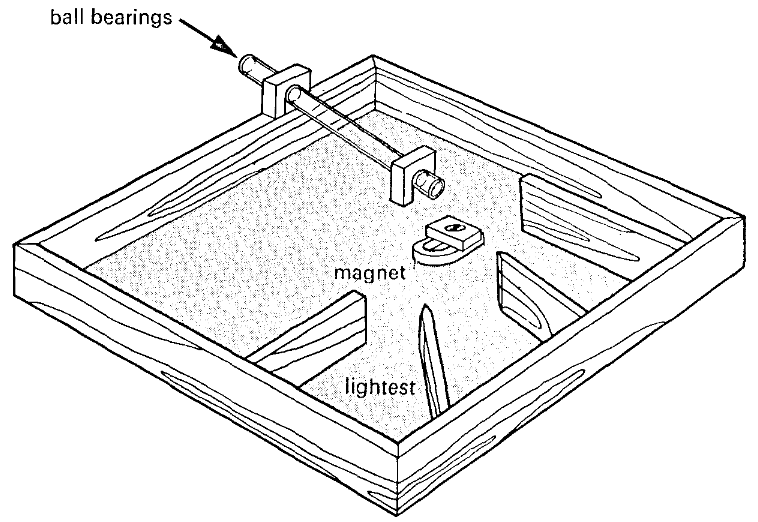
\includegraphics[width=0.99\textwidth]{images/nuffield.png}
  \caption[Funktionsmodell eines Massenspektrometers der Nuffield Foundation]{Funktionsmodell eines Massenspektrometers der Nuffield Foundation. Kugellager-Kugeln rollen durch ein Glasrohr nach unten auf die Platte, wo sie von einem Magneten gestreut werden. Die leichtesten Kugeln werden am Weitesten abgelenkt (entnommen aus \cite[S\,262]{Nuffield1970}).}
  \label{fig:nuffsaid}
  \vspace{-0pt}
\end{figure}

\noindent\textsc{Bühler/Graf}, die bereits im zweiten Satz ihres Artikels \textsc{J. J. Thomson} mit dessen Sohn verwechseln,\footfullcite[vgl.][S.\,33]{Graf2002} befüllen Tischtennisbälle mit Eisenwolle und Nylonwatte, um unterscheidbare Massen-Ladungs-Verhältnisse nachzuahmen.
Der leere Tischtennisball wird durch die Magnetanordnung nicht aus seiner Startrichtung ausgelenkt, der Ball mit $\SI{3}{\gram}$ Eisenwollfüllung wird am Stärksten abgelenkt und der Ball mit jeweils $\SI{3}{\gram}$ Eisenwolle- und Nyolonwattefüllung wird leicht abgelenkt (vgl. Abbildung \ref{fig:graf}).
Sie umreißen ihren Versuch unter anderem mit den Adjektiven \textit{anschaulich}, \textit{objektiv} und \textit{begreifbar}.

%% Autor: Björn Ritterbecks 
%% Letzte Aenderung: 15.06.2016 
\thisfloatsetup{%
  capbesidewidth=\marginparwidth}
\begin{figure}[htbp]
\centering
%\sansmath
 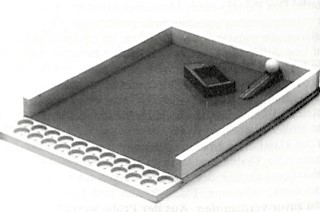
\includegraphics[width=0.99\textwidth]{images/graf.jpg}
  \caption[Funktionsmodell eines Massenspektrometers von Bühler und Graf]{Funktionsmodell eines Massenspektrometers von Bühler und Graf. Tischtennisbälle werden durch eine kleine Bohrung mit Eisenwolle und/oder Nylonwatte befüllt, um Masse-Ladungs-Verhältnisse nachzuahmen (entnommen aus \cite[S\,34]{Graf2002}).}
  \label{fig:graf}
  \vspace{-0pt}
\end{figure}
\noindent Als Motivation für die Neuauflage des Versuches schreiben sie jedoch der Version von 1970 zwei Probleme zu, welche diese gar nicht haben sollte: Sowohl der ">verschiedene Rollwiderstand"<\footcite[vgl.][S.\,35]{Graf2002} als auch das Fehlen der Entmagnetisierung der Kugeln wird moniert, indem auf \textsc{Nuffield} verwiesen wird. Dort heißt es jedoch ">the ball bearings that stick to the magnet will become magnetized and should be dropped several times to demagnetize them."<\footcite[S.\,264]{Nuffield1970} Es wird bei \textsc{Nuffield} mit Kugellagern gearbeitet, die zu den rotationssymmetrischsten und glattesten Kugeln gehören, die man kaufen kann (überdies ist der Rollwiderstand noch von dem Material abhängig, was jedoch bei allen Kugeln \textit{Stahl} ist). Zudem führt das Fallenlassen der Kugeln bereits zu einer Auflösung der \textit{Weiß'schen Bezirke},\footcite[vgl.][S.\,13]{Mais2014} da die Ausrichtung der magnetischen Spins sehr schwach ist.
  \thisfloatsetup{
  capbesidewidth=\marginparwidth,}
\begin{table}[htb]
\centering
%\sffamily,
\small
%\sansmath
\arrayrulecolor{white}
\vspace{0.2cm}
  \rowcolors{2}{halfgray!15}{halfgray!5}
 \setlength{\extrarowheight}{.0em}
			\begin{tabularx}{0.99\textwidth}{l*{1}{>{\RaggedRight\arraybackslash}X}}		
\rowcolor{mycolor}\multicolumn{1}{l}{{\color{white}\textbf{Sektorfeld-Massenspektrometer}}}&  \multicolumn{1}{l}{{\color{white}\textbf{Modellversuch}}}\\
Atome & Acrylkugeln\\
Ionen & mit Eisenwolle gefüllte Kugeln\\
Beschleunigereinheit & Schiefe Ebene\\
Massenanalysator  & Permanentmagnet\\
homogenes Magnetfeld & inhomogenes Magnetfeld\\
Detektor & Röhrensystem\\\bottomrule[5pt]
Elektrisches Feld  & Gravitationsfeld\\
Lorentzkraft $F_\mathrm{L}$& Magnetische Kraft $F_\mathrm{m}$ (sic!)\\
Ionenladung $q$ & Volumen $V_\mathrm{EW}$ der Eisenwolle\\
Elementarladung $e$  & Feste Volumeneinheit $V=\frac{\sfrac{1}{3}\si{\gram}}{\rho_\mathrm{EW}}$\\
Ladung $q=n\cdot e$  & $n\cdot V$\\
		\end{tabularx}
		\caption[Analogien Modellversuch Magnete]{Die Analogie-Zuweisungen nach \textsc{Böhmer} und \textsc{Mais} für den Analogieversuch mit einer Magnetanordnung. Im oberen Teil der Tabelle sind die objektalen, in der unteren Hälfte die begrifflichen Zuordnungen aufgelistet (nach \cite[S.\,16]{Mais2014}).} 
		\label{tab:mais}		
		\end{table}

\noindent Die Hauptprobleme des \textit{Magnetmodells} sind jedoch sowohl die Inhomogenität des magnetischen Feldes, welche eine mathematische Beschreibung der Kugelbewegung nahezu unmöglich macht, als auch die Nichtberücksichtung unterschiedlicher Trägheitsmomente. Bei makroskopischen Modellversuchen können die Kugeln nicht mehr als Punktmassen, was mit den Berechnungen in Abschnitt \ref{sec:fields2} bereits gezeigt wurde, genähert werden. 

Durch \textsc{Böhmer} und \textsc{Mais} wurde dieser Versuch durch eine verbesserte Magnetanordnung und eine bogenförmige Detektoranordnung verbessert. Die abschließenden Analogiebetrachtungen der Examensarbeit von \textsc{Axel Mais} sind in Tabelle \ref{tab:mais} wiedergegeben.


\subsection{Gebläse}

Ein Funktionsmodell zur Massenspektrometrie, welches Gebläse als Analysatoren einsetzt, wurde 1987 im Rahmen einer Zulassungsarbeit von \textsc{Elisabeth Schilling} an der LMU München angefertigt. Der Archivierungszeitraum ist zwar bereits überschritten und damit die Arbeit für alle weiteren Recherchen verloren, jedoch sind die wichtigsten Ergebnisse in einem Artikel der Zeitschrift \textit{der mathematische und naturwissenschaftliche Unterricht} enthalten\footfullcite[vgl.]{Schilling1987}, der dem Verfasser freundlicherweise von Professor Klaus Wendt der Johannes Gutenberg Universität Mainz zugeschickt wurde.

Dieses Funktionsmodell (siehe Abbildung \ref{fig:mnu}) ist die einzig bekannte Ausführung eines geschwindigkeitsfokussierenden Spektrometers. 

Mittels einer $\SI{30}{\centi\metre}$ langen, v-förmigen Rampe, welche eine Steigung von ca. $\SI{20}{\degree}$ besitzt, werden $\SI{20}{\milli\metre}$ große Stahl-, Aluminium- und Plexiglaskugeln beschleunigt. Über eine Platte mit sehr geringer Neigung (ungefähr $1:100$) werden die Kugeln nach ihrer Geschwindigkeit aufgespalten. Je langsamer die Kugel, desto mehr Zeit hat die Erdbeschleunigung, sie abzulenken (vgl. \ref{sec:gravity}). Eine weitere Platte --- diesmal waagerecht montiert --- schließt an die Erste an. An ihrem oberen Ende ist ein Gebläse angebracht, das zu einer Auslenkung der rollenden Kugeln in Abhängigkeit von ihrem Impuls sorgt. Wie mathematisch gezeigt werden kann, kommt es zu einer Fokussierung von Kugeln gleicher Masse und unterschiedlicher Starthöhe. Hierzu sei unter Berücksichtigung der Abschnitte \ref{sec:fields2} und \ref{sec:aston} auf die weitere Analyse in \ref{sec:voraus} verwiesen.

\textsc{Schilling} äußert auch die Gewissheit, dass sich das Funktionsmodell dazu eignet, komplexere Eigenschaften eines Massenspektrometers, wie beispielsweise das Auflösungsvermögen, zu untersuchen.\footcite[vgl.][S.\,37]{Schilling1987}
%% Autor: Björn Ritterbecks 
%% Letzte Aenderung: 15.06.2016 
\thisfloatsetup{%
  capbesidewidth=\marginparwidth,
    capbesideposition=top,
    postcode=flushupp}
\begin{figure*}[htbp]
\centering
%\sansmath
 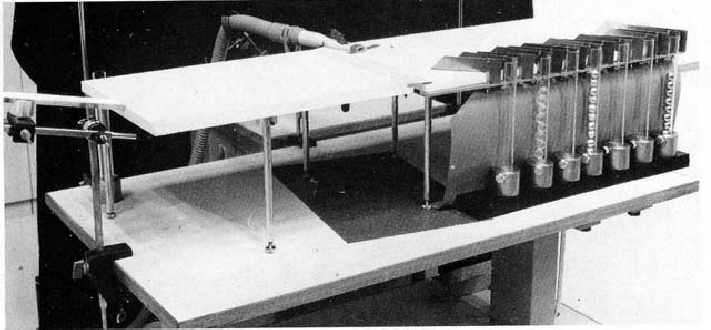
\includegraphics[width=0.99\fulllinewidth]{images/mnu.png}
  \caption[Analogieversuch zu Massenspektrometrie nach \textsc{Luchner}, \textsc{Degner} und \textsc{Schilling} ]{\protect\rule{0cm}{7.6cm}Mechanisches Funktionsmodell eines geschwindigkeitsfokussierenden Massenspektrographen nach \textsc{Schilling} et al.: Kugeln unterscheidbarer Dichte werden die v-förmige Rampe an der linken Seite heruntergerollt, wo sie auf einer schiefen Ebene nach ihrer Geschwindigkeit sortiert werden. Auf der rechten Seite sorgt das Strömungsfeld eines Gebläses für eine Aufspaltung nach den Impulsen (entnommen aus \cite[S\,35]{Schilling1987}).}
  \label{fig:mnu}
  \vspace{-0pt}
\end{figure*}

Abschließend wird anhand von \textit{Stroboskopaufnahmen} --- übrigens ein hervorragendes Mittel zur Visualisierung von Bewegungsprozessen --- eine quantitative Untersuchung der Impulsänderungen $\Delta p$ in Abhängigkeit von der Starthöhe durchgeführt. Hierbei wird ausgenutzt, dass 
\begin{equation}
\begin{alignedat}{2}
\label{eq:impulsaenderung}
\boldsymbol{F}&=m\boldsymbol{\ddot{r}}\\
\Rightarrow \int \boldsymbol{F}\mathrm{d}t &=m\boldsymbol{\dot{r}}=\Delta p
\end{alignedat}
\end{equation} 
gilt, d.\,h. die Krafteinwirkung eines Feldes --- über die Zeit der Einwirkung integriert --- ergibt eine Impulsänderung.

Wenn demnach bekannt ist, wie groß die Krafteinwirkung des Gebläses in Beziehung zu der Entfernung und wie hoch die Geschwindigkeit der sich bewegenden Masse ist, so kann über eine Umformung von \eqref{eq:impulsaenderung} mit der Setzung $\boldsymbol{r}=\boldsymbol{\dot{r}}t$ (vgl. \eqref{eq:bewegung4}) das Integral der Kraft des Strömungsfeldes über dem Abstand von der Mittelachse $x$ berechnet werden, woraus man mittels Division durch die Kugelgeschwindigkeit die Impulsänderung erhält.

\section{Umsetzung}
\label{sec:umsetzung}
Diese Arbeit sollte ursprünglich das Analogiemodell von \textsc{Mais} zu einem Praktikumsversuch weiterentwickeln. Nach einem Hinweis von Frau Professor \textsc{Heidrun Heinke}, dass --- in Anbetracht der Unzulänglichkeiten des Magnetmodells --- auch ein Gebläse als Analysatoreinheit verwendet werden könne, wurde der ursprüngliche Versuchsaufbau nach anfänglichen Testmessungen mit einem handelsüblichen Föhn verworfen (siehe Abschnitt \ref{sec:analysatoren1}).

Aufgrund der Oberflächenähnlichkeit des Funktionsmodells aus \textcite{Schilling1987} mit einem Sektorfeld-Massenspektrometer wird jedoch \textsc{Böhmer} in diesem Punkte gefolgt.\vspace*{-0.4cm}\footcite[vgl. die ausführliche Begründung bei][S.\,26--27]{Boehmer2013}\vspace*{0.4cm} Aus diesem Grund wurde der \textsc{Aston}'sche Massenspektograph als Inkarnation eines EB-Spek{\-}tro{\-}me{\-}ters in Abschn. \ref{sec:aston} auf seine Ablenkung hin untersucht. 

Nach Auswertung der physikalischen Hintergründe wird anhand des zu berücksichtigenden Schemas für wertschöpfende Analogexperimente von \textsc{Kircher} (Tab.\,\ref{tab:ana1}, insbesondere Schritte 3 und 4)  ein Vorschlag die Objektebene betreffend gemacht, welcher zusammengefasst in Tabelle \ref{tab:ana2} zu überblicken ist.

  \thisfloatsetup{
  capbesidewidth=\marginparwidth,}
\begin{table}[htb]
\centering
%\sffamily,
\small
%\sansmath
\arrayrulecolor{white}
\vspace{0.2cm}
  \rowcolors{2}{halfgray!15}{halfgray!5}
 \setlength{\extrarowheight}{.0em}
			\begin{tabularx}{0.99\textwidth}{l*{1}{>{\RaggedRight\arraybackslash}X}}		
\rowcolor{mycolor}\multicolumn{1}{l}{{\color{white}\textbf{Sektorfeld-Massenspektrometer}}}&  \multicolumn{1}{l}{{\color{white}\textbf{Funktionsmodell}}}\\
verschiedene Atome & Kugeln unterscheidbarer Dichte\\
ionisierte Atome & Verschiedene Kugelquerschnittsflächen\\
Hochvakuum & Leerer Experimentiertisch\\
Beschleunigungsspannung & Startrampe mit waagerechtem Auslauf\\
Blendensystem & Schmale Platte lässt nicht alle Geschwindigkeiten zu\\
Analysator I  & Schiefe Ebene\\
Analysator II  & Haartrockner\\
Photoplatte & Auffangbehälter\\
		\end{tabularx}
		\caption[Objektebene der Analogie]{Die Objektebene des Analogieversuches mit einer schiefen Ebene und einem Haartrockner als Massenanalysatoren (eigene Darstellung).} 
		\label{tab:ana2}		
		\end{table}

\noindent Die Anforderungen an die Kugeln sind zwei Gestalt: Erstens muss die Möglichkeit bestehen, verschiedenartige Dichten zu verwenden. Des Weiteren besteht ein Bedarf an einer Projektionsfläche $A_\mathrm{proj}$, welche bestenfalls als Analogon der \textit{Quantelung} von Ladung herhalten kann, indem eine Querschnittsfläche $A_\mathrm{min}$ festgelegt wird, für die weitere Kugelgrößen anhand der Überlegung
\begin{equation}
\label{eq:umsetzung1}
A_i=A_\mathrm{min}\cdot (i+1),\qquad i \in \mathbb{N}\text{ mit }A_i=\uppi r_i^2 
\end{equation} 
festgelegt werden. Dies ist zum Beispiel mit den Radien $r_0=\SI{10}{\milli\metre}$, $r_1=\SI{14}{\milli\metre}$, $r_2=\SI{17}{\milli\metre}$ und $r_3=\SI{20}{\milli\metre}$ erfüllt.

Eine Geschwindigkeitsfokussierung ist nach \ref{sec:aston} nur möglich, wenn die Geschwindigkeiten im Strömungsfeld nicht zu weit auseinander liegen. Wird die Plattengröße klein genug gewählt, so besitzen sämtliche detektierbaren Kugeln gleicher Masse eine Breite $\Delta v$, auf der die Spuren der Kugeln sich nahezu schneiden.

Durch die Auswertung der ersten Messung mit einem Gebläse als Massenanalysator ist augenscheinlich geworden, dass bei den vorhandenen Rampen ca. $\sfrac{1}{4}$ der potentiellen Energie, die durch die Starthöhe vorgegeben wird, nach dem Übergang von Rampe zu Platte nicht in kinetische Energie umgesetzt wird, bzw. dass diese durch ein \textit{Aufprallen} auf der ebenen Fläche verloren geht. Damit ist dieser Energieverlust wesentlich höher als experimentell und theoretisch bestimmte Luftreibungs- und Rollreibungsverluste (ausführlicher inklusive Messdaten siehe Kapitel \ref{kap:5}).

Über einen Vergleich der theoretischen Abschnitte \ref{sec:force1} und \ref{sec:fields2} kann die schiefe Ebene als erster Teil der Massenanalyse eins zu eins auf das elektrische Feld übertragen werden, da Coulombkraft und Gravitationskraft jeweils zu einer Beschleunigung führen, die mit dem Abstand $s$\footnote{Im Folgenden gilt $a \mathop{\hat{=}} $ \textsw{Beschleunigung}, $v \mathop{\hat{=}} $ \textsw{Geschwindigkeit} und $s \mathop{\hat{=}} $ \textsw{Abstand}, um keine doppelte Variablenbelegung zu haben.} zum Quadrat abnimmt, linear mit einem Faktor ($\epsilon_0$ und $G$) skaliert und sich die Masse $m$ des Gravitationspotentials mit der Ladung $q$ des Coulompotentials ersetzen lässt.

Über den zweiten Teil des Analysators sind nur die Erkenntnisse von \textcite{Schilling1987} bekannt. Daher folgt an dieser Stelle die Untersuchung des Haartrockners. In Tabelle \ref{tab:ana3} werden die Ergebnisse jedoch der Übersichtlichkeit halber bereits mit aufgeführt.

  \thisfloatsetup{
  capbesidewidth=\marginparwidth,}
\begin{table}[htb]
\centering
%\sffamily,
\small
%\sansmath
\arrayrulecolor{white}
\vspace{0.2cm}
  \rowcolors{2}{halfgray!15}{halfgray!5}
 \setlength{\extrarowheight}{.40em}
			\begin{tabularx}{0.99\textwidth}{X*{1}{>{\RaggedRight\arraybackslash}X}}		
\rowcolor{mycolor}\multicolumn{1}{l}{{\color{white}\textbf{Sektorfeld-Massenspektrometer}}}&  \multicolumn{1}{l}{{\color{white}\textbf{Funktionsmodell}}}\\
Coulomb-Potential $\phi_\mathrm{Coul} =\frac{1}{4\uppi\epsilon_0}\frac{Q}{r}$ & Gravitationspotential $\phi_\mathrm{Grav}=-G\frac{m}{r}$\\
Elementarladung $q$ & Projektionsfläche $A_\mathrm{min}=\uppi r_\mathrm{min}^2$\\
Gesamtladung $Q=n\cdot q$ & Projektionsfläche $A_i=i\cdot A_\mathrm{min}$\\ 
Potentielle Energie $qU_\mathrm{B}$& Potentielle Energie $mgh$\\
Kinetische Energie $\frac{1}{2}mv^2$& Kinetische Energie $\frac{7}{10}mv^2$\\
Lorentzkraft $F_\mathrm{L}=qvB$ & Strömungswiderstandskraft $F_\mathrm{W}=c_\mathrm{W}A\frac{\rho v^2}{2}$\\
Anzahl detektierter Impulse für $\sfrac{m}{q}=j$ & Aufgefangene Kugeln in Detektor $j$\\
		\end{tabularx}
		\caption[Begriffsebene der Analogie]{Übersicht der begrifflichen Analogien zwischen dem Primär- und Sekundärbereich bei Nutzung einer schiefen Ebene und eines Föhns als Massenanalysatoren. Da bei dem Vergleich zwischen den Lernbereichen der Radius $r$ auftaucht, wird ab dieser Stelle für die Geschwindigkeit $v$ verwendet (eigene Darstellung).} 
		\label{tab:ana3}		
		\end{table}

\section{Gebläse}
\label{sec:analysatoren1}

Obwohl die Überprüfung der erarbeiteten Analogie-Setzungen erst in Kapitel \ref{kap:5} durchgeführt werden wird, muss zuvorderst der gewählte Analysator in Form eines durch einen Föhn hervorgerufenen Strömungsfeldes überprüft werden. Die Messergebnisse werden anschließend mit den abschließenden Werten von \textcite[S.\,53--66]{Mais2014} verglichen.

Hierbei wird auch die Forderung nach einem \textit{gebogenen} Detektor umgesetzt, da die Aufspaltung der Kugeln als Winkelstreuung mit einem festen Mittelpunkt bei $(x, y)\tran$ = $(x, y)\tran (F_\mathrm{max})$, d.\,h. im Punkte der maximalen Krafteinwirkung, gesehen werden kann.

%% Autor: Björn Ritterbecks 
%% Letzte Aenderung: 15.06.2016 
\thisfloatsetup{%
  capbesidewidth=\marginparwidth}
\begin{figure}[htb!p]
\centering
%\sansmath
 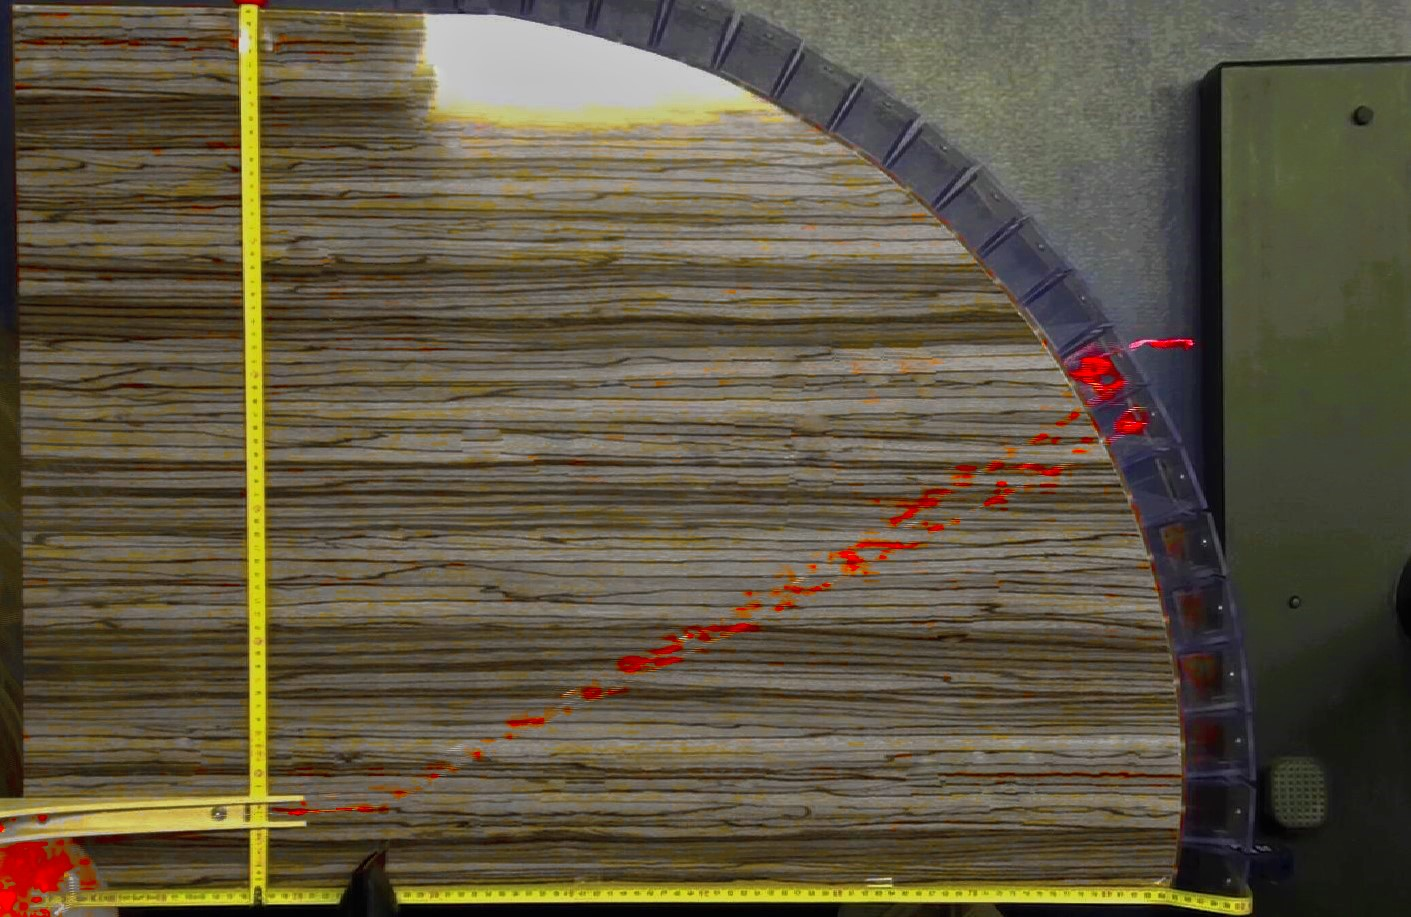
\includegraphics[width=0.99\textwidth]{images/strobe1.jpg}
  \caption[Exemplarische Stroboskopaufnahme der ersten Messreihe]{Exemplarisches Bildschirmfoto mit Stroboskopfilter der ersten Messreihe. Wegen des geringen Kontrastes zwischen den roten Kugeln und der bräunlichen Arbeitsplatte werden Farbfilter angewendet, um die Bahnkurven besser erkennbar zu machen. Bei der Auswertung einzelner Bilder in der Software \textit{Tracker} sind die Kugeln bis auf eine Bewegungsverzerrung gut erkennbar.}
  \label{fig:strobe1}
  \vspace{-0pt}
\end{figure}

Abbildung \ref{fig:strobe1} zeigt den rudimentären Versuchsaufbau nebst der stoboskopischen Aufnahme zweier Kugelbahnen. Ein im Baumarkt erhältliches Reststück einer Arbeitsplatte von etwa $\SI{1.2}{\metre}$ mal $\SI{0.8}{\metre}$ wurde bogenförmig ausgesägt, wobei der Ablenkwinkel von $\SI{0}{\degree}$ auf einer Achse mit der Startrampe liegt. Im Zuge dieser Videoauswertung wird auch die Güte der Rampe untersucht. Diese besitzt eine durch das bloße Auge zu erkennende Asymmetrie, welche den abrollenden Kugeln eine Rotation in $y$-Richtung mitgibt (das im Bildschirmfoto obere Segment der Startvorrichtung ist kürzer als das untere).

Vor den eigentlichen Auswertungen muss daher erstmal ohne angeschalteten Föhn die \textit{Nulllinie} bestimmt werden. Hierzu werden die $10$ von \textcite[S.\,34]{Mais2014} präparierten Kugeln jeweils fünf mal von dem Anschlag bei einer Starthöhe von $h=\SI{55}{\milli\metre}$ abgerollt. Für sämtliche Videoauswertungen wird auf die in der Software \textit{Tracker} bestimmten Koordinaten eine Unsicherheit von $\SI{0.5}{\centi\metre}$ in beide Richtungen angenommen.

Aufgrund der großen Datenmenge werden an dieser Stelle nur die Bewegungen der ersten Kugel tabellarisch und als Diagramm dargestellt. Bei den weiteren Videoauswertungen wird nur noch die Detektionshäufigkeit in Behälter $i$ betrachtet (siehe Tabelle \ref{tab:nullpunkt1}). 

Es ist auch von Interesse, ob sich die Kugeln hinter der Stelle der Krafteinwirkung auf einer Geraden bewegen, d.\,h. ob die Platte trotz der Ungenauigkeit von Wasserwaagen horizontal ausgerichtet ist. Dazu eignet sich der \textit{Bravais-Pearson-Korrelationskoeffizient}, der genau dann einen der Werte $\pm 1$ annimmt, wenn sich die Messdaten auf einer Geraden mit positiver/negativer Steigung befinden.\footfullcite[vgl.][S.\,111]{Cramer2008} Der B-P-Koeffizient ist über den Quotienten der \textit{empirischen Kovarianz} $s_{xy}$ durch das Produkt der Standardabweichungen $s_x$, $s_y$ (oder \textit{empirische Varianzen}) definiert:
\begin{equation}
\label{eq:b-p-k}
r_{xy}=\frac{s_{xy}}{s_xs_y}=\frac{\sum\limits_{i=1}^{n}(x_i-\overline{x})(y_i-\overline{y})}{\sqrt{\sum\limits_{i=1}^{n}(x_i-\overline{x}^2)}\sqrt{\sum\limits_{i=1}^{n}(y_i-\overline{y})^2}}\\
\end{equation}

  \thisfloatsetup{
  capbesidewidth=\marginparwidth,
}
\begin{table}[!p]
\centering
%\sffamily,
\small
%\sansmath
\arrayrulecolor{white}
\setlength{\arrayrulewidth}{2pt}
\vspace{0.2cm}
  \rowcolors{2}{halfgray!15}{halfgray!5}
 \setlength{\extrarowheight}{.00em}\subfloat{
			\begin{tabularx}{0.99\fulllinewidth}{X*{6}{>{\RaggedLeft\arraybackslash}X}}		
\rowcolor{mycolor} &  \multicolumn{2}{|c}{{\color{white}\textbf{Bahn 1}}} &  \multicolumn{2}{|c}{{\color{white}\textbf{Bahn 2}}}&\multicolumn{2}{|c}{{\color{white}\textbf{Bahn 3}}}\\
\rowcolor{mycolor} \multirow{-2}{*}{{\color{white}\textbf{$\boldsymbol{t}$ in $\boldsymbol{\si{\second}}$}}}& \multicolumn{1}{|r}{{\color{white}\textbf{$\boldsymbol{x}$ in $\boldsymbol{\si{\milli\metre}}$}}}&  \multicolumn{1}{r}{{\color{white}\textbf{$\boldsymbol{y}$ in $\boldsymbol{\si{\milli\metre}}$}}} & \multicolumn{1}{|r}{{\color{white}\textbf{$\boldsymbol{x}$ in $\boldsymbol{\si{\milli\metre}}$}}}&  \multicolumn{1}{r}{{\color{white}\textbf{$\boldsymbol{y}$ in $\boldsymbol{\si{\milli\metre}}$}}}&\multicolumn{1}{|r}{{\color{white}\textbf{$\boldsymbol{x}$ in $\boldsymbol{\si{\milli\metre}}$}}}&  \multicolumn{1}{r}{{\color{white}\textbf{$\boldsymbol{y}$ in $\boldsymbol{\si{\milli\metre}}$}}}\\
0,00	& \multicolumn{1}{|r}{	-53	$\pm$ 5	}&	-1	$ \pm$ 5	 & \multicolumn{1}{|r}{	-68	$ \pm$ 5	}&	-7	$ \pm$ 5	 & \multicolumn{1}{|r}{	-49	$ \pm$ 5	}&	-5	$ \pm$ 5	\\
0,04	& \multicolumn{1}{|r}{	-24	$\pm$ 5	}&	-2	$ \pm$ 5	 & \multicolumn{1}{|r}{	-35	$ \pm$ 5	}&	-5	$ \pm$ 5	 & \multicolumn{1}{|r}{	-17	$ \pm$ 5	}&	-4	$ \pm$ 5	\\
0,08	& \multicolumn{1}{|r}{	14	$\pm$ 5	}&	1	$ \pm$ 5	 & \multicolumn{1}{|r}{	-1	$ \pm$ 5	}&	-2	$ \pm$ 5	 & \multicolumn{1}{|r}{	14	$ \pm$ 5	}&	-5	$ \pm$ 5	\\
0,12	& \multicolumn{1}{|r}{	40	$\pm$ 5	}&	2	$ \pm$ 5	 & \multicolumn{1}{|r}{	29	$ \pm$ 5	}&	-1	$ \pm$ 5	 & \multicolumn{1}{|r}{	61	$ \pm$ 5	}&	-2	$ \pm$ 5	\\
0,16	& \multicolumn{1}{|r}{	68	$\pm$ 5	}&	4	$ \pm$ 5	 & \multicolumn{1}{|r}{	50	$ \pm$ 5	}&	-1	$ \pm$ 5	 & \multicolumn{1}{|r}{	70	$ \pm$ 5	}&	-2	$ \pm$ 5	\\
0,20	& \multicolumn{1}{|r}{	101	$\pm$ 5	}&	8	$ \pm$ 5	 & \multicolumn{1}{|r}{	83	$ \pm$ 5	}&	0	$ \pm$ 5	 & \multicolumn{1}{|r}{	101	$ \pm$ 5	}&	0	$ \pm$ 5	\\
0,24	& \multicolumn{1}{|r}{	131	$\pm$ 5	}&	8	$ \pm$ 5	 & \multicolumn{1}{|r}{	120	$ \pm$ 5	}&	2	$ \pm$ 5	 & \multicolumn{1}{|r}{	132	$ \pm$ 5	}&	2	$ \pm$ 5	\\
0,28	& \multicolumn{1}{|r}{	154	$\pm$ 5	}&	10	$ \pm$ 5	 & \multicolumn{1}{|r}{	143	$ \pm$ 5	}&	4	$ \pm$ 5	 & \multicolumn{1}{|r}{	162	$ \pm$ 5	}&	5	$ \pm$ 5	\\
0,32	& \multicolumn{1}{|r}{	186	$\pm$ 5	}&	13	$ \pm$ 5	 & \multicolumn{1}{|r}{	169	$ \pm$ 5	}&	7	$ \pm$ 5	 & \multicolumn{1}{|r}{	193	$ \pm$ 5	}&	6	$ \pm$ 5	\\
0,36	& \multicolumn{1}{|r}{	216	$\pm$ 5	}&	16	$ \pm$ 5	 & \multicolumn{1}{|r}{	203	$ \pm$ 5	}&	8	$ \pm$ 5	 & \multicolumn{1}{|r}{	222	$ \pm$ 5	}&	10	$ \pm$ 5	\\
0,40	& \multicolumn{1}{|r}{	246	$\pm$ 5	}&	17	$ \pm$ 5	 & \multicolumn{1}{|r}{	234	$ \pm$ 5	}&	8	$ \pm$ 5	 & \multicolumn{1}{|r}{	247	$ \pm$ 5	}&	11	$ \pm$ 5	\\
0,44	& \multicolumn{1}{|r}{	276	$\pm$ 5	}&	18	$ \pm$ 5	 & \multicolumn{1}{|r}{	262	$ \pm$ 5	}&	10	$ \pm$ 5	 & \multicolumn{1}{|r}{	283	$ \pm$ 5	}&	12	$ \pm$ 5	\\
0,48	& \multicolumn{1}{|r}{	300	$\pm$ 5	}&	20	$ \pm$ 5	 & \multicolumn{1}{|r}{	292	$ \pm$ 5	}&	12	$ \pm$ 5	 & \multicolumn{1}{|r}{	309	$ \pm$ 5	}&	14	$ \pm$ 5	\\
0,52	& \multicolumn{1}{|r}{	321	$\pm$ 5	}&	19	$ \pm$ 5	 & \multicolumn{1}{|r}{	321	$ \pm$ 5	}&	13	$ \pm$ 5	 & \multicolumn{1}{|r}{	341	$ \pm$ 5	}&	16	$ \pm$ 5	\\
0,56	& \multicolumn{1}{|r}{	354	$\pm$ 5	}&	22	$ \pm$ 5	 & \multicolumn{1}{|r}{	347	$ \pm$ 5	}&	14	$ \pm$ 5	 & \multicolumn{1}{|r}{	366	$ \pm$ 5	}&	19	$ \pm$ 5	\\
0,60	& \multicolumn{1}{|r}{	388	$\pm$ 5	}&	24	$ \pm$ 5	 & \multicolumn{1}{|r}{	381	$ \pm$ 5	}&	14	$ \pm$ 5	 & \multicolumn{1}{|r}{	398	$ \pm$ 5	}&	20	$ \pm$ 5	\\
0,64	& \multicolumn{1}{|r}{	417	$\pm$ 5	}&	28	$ \pm$ 5	 & \multicolumn{1}{|r}{	411	$ \pm$ 5	}&	16	$ \pm$ 5	 & \multicolumn{1}{|r}{	429	$ \pm$ 5	}&	25	$ \pm$ 5	\\
0,68	& \multicolumn{1}{|r}{	444	$\pm$ 5	}&	28	$ \pm$ 5	 & \multicolumn{1}{|r}{	436	$ \pm$ 5	}&	18	$ \pm$ 5	 & \multicolumn{1}{|r}{	458	$ \pm$ 5	}&	31	$ \pm$ 5	\\
0,72	& \multicolumn{1}{|r}{	479	$\pm$ 5	}&	25	$ \pm$ 5	 & \multicolumn{1}{|r}{	464	$ \pm$ 5	}&	22	$ \pm$ 5	 & \multicolumn{1}{|r}{	483	$ \pm$ 5	}&	31	$ \pm$ 5	\\
0,76	& \multicolumn{1}{|r}{	499	$\pm$ 5	}&	31	$ \pm$ 5	 & \multicolumn{1}{|r}{	496	$ \pm$ 5	}&	24	$ \pm$ 5	 & \multicolumn{1}{|r}{	509	$ \pm$ 5	}&	35	$ \pm$ 5	\\
0,80	& \multicolumn{1}{|r}{	529	$\pm$ 5	}&	29	$ \pm$ 5	 & \multicolumn{1}{|r}{	524	$ \pm$ 5	}&	24	$ \pm$ 5	 & \multicolumn{1}{|r}{	541	$ \pm$ 5	}&	40	$ \pm$ 5	\\
		\end{tabularx}}
		\\
		\subfloat{\begin{tabularx}{0.99\textwidth}{X*{4}{>{\RaggedLeft\arraybackslash}X}}		
		\rowcolor{mycolor} &  \multicolumn{2}{|c}{{\color{white}\textbf{Bahn 4}}} &  \multicolumn{2}{|c}{{\color{white}\textbf{Bahn 5}}}\\
		\rowcolor{mycolor} \multirow{-2}{*}{{\color{white}\textbf{$\boldsymbol{t}$ in $\boldsymbol{\si{\second}}$}}}& \multicolumn{1}{|r}{{\color{white}\textbf{$\boldsymbol{x}$ in $\boldsymbol{\si{\milli\metre}}$}}}&  \multicolumn{1}{r}{{\color{white}\textbf{$\boldsymbol{y}$ in $\boldsymbol{\si{\milli\metre}}$}}} & \multicolumn{1}{|r}{{\color{white}\textbf{$\boldsymbol{x}$ in $\boldsymbol{\si{\milli\metre}}$}}}&  \multicolumn{1}{r}{{\color{white}\textbf{$\boldsymbol{y}$ in $\boldsymbol{\si{\milli\metre}}$}}}\\
0,00	& \multicolumn{1}{|r}{	-25	$\pm$ 5	}&	-8	$ \pm$ 5	 & \multicolumn{1}{|r}{	-5	$ \pm$ 5	}&	1	$ \pm$ 5	\\
0,04	& \multicolumn{1}{|r}{	8	$\pm$ 5	}&	-5	$ \pm$ 5	 & \multicolumn{1}{|r}{	26	$ \pm$ 5	}&	6	$ \pm$ 5	\\
0,08	& \multicolumn{1}{|r}{	41	$\pm$ 5	}&	-8	$ \pm$ 5	 & \multicolumn{1}{|r}{	58	$ \pm$ 5	}&	10	$ \pm$ 5	\\
0,12	& \multicolumn{1}{|r}{	72	$\pm$ 5	}&	-5	$ \pm$ 5	 & \multicolumn{1}{|r}{	86	$ \pm$ 5	}&	11	$ \pm$ 5	\\
0,16	& \multicolumn{1}{|r}{	100	$\pm$ 5	}&	-2	$ \pm$ 5	 & \multicolumn{1}{|r}{	117	$ \pm$ 5	}&	12	$ \pm$ 5	\\
0,20	& \multicolumn{1}{|r}{	126	$\pm$ 5	}&	0	$ \pm$ 5	 & \multicolumn{1}{|r}{	147	$ \pm$ 5	}&	12	$ \pm$ 5	\\
0,24	& \multicolumn{1}{|r}{	161	$\pm$ 5	}&	-1	$ \pm$ 5	 & \multicolumn{1}{|r}{	175	$ \pm$ 5	}&	13	$ \pm$ 5	\\
0,28	& \multicolumn{1}{|r}{	185	$\pm$ 5	}&	-2	$ \pm$ 5	 & \multicolumn{1}{|r}{	208	$ \pm$ 5	}&	16	$ \pm$ 5	\\
0,32	& \multicolumn{1}{|r}{	219	$\pm$ 5	}&	2	$ \pm$ 5	 & \multicolumn{1}{|r}{	237	$ \pm$ 5	}&	14	$ \pm$ 5	\\
0,36	& \multicolumn{1}{|r}{	244	$\pm$ 5	}&	4	$ \pm$ 5	 & \multicolumn{1}{|r}{	265	$ \pm$ 5	}&	17	$ \pm$ 5	\\
0,40	& \multicolumn{1}{|r}{	273	$\pm$ 5	}&	5	$ \pm$ 5	 & \multicolumn{1}{|r}{	292	$ \pm$ 5	}&	20	$ \pm$ 5	\\
0,44	& \multicolumn{1}{|r}{	304	$\pm$ 5	}&	8	$ \pm$ 5	 & \multicolumn{1}{|r}{	327	$ \pm$ 5	}&	20	$ \pm$ 5	\\
0,48	& \multicolumn{1}{|r}{	330	$\pm$ 5	}&	10	$ \pm$ 5	 & \multicolumn{1}{|r}{	348	$ \pm$ 5	}&	25	$ \pm$ 5	\\
0,52	& \multicolumn{1}{|r}{	359	$\pm$ 5	}&	12	$ \pm$ 5	 & \multicolumn{1}{|r}{	378	$ \pm$ 5	}&	26	$ \pm$ 5	\\
0,56	& \multicolumn{1}{|r}{	393	$\pm$ 5	}&	13	$ \pm$ 5	 & \multicolumn{1}{|r}{	405	$ \pm$ 5	}&	28	$ \pm$ 5	\\
0,60	& \multicolumn{1}{|r}{	418	$\pm$ 5	}&	14	$ \pm$ 5	 & \multicolumn{1}{|r}{	437	$ \pm$ 5	}&	29	$ \pm$ 5	\\
0,64	& \multicolumn{1}{|r}{	442	$\pm$ 5	}&	17	$ \pm$ 5	 & \multicolumn{1}{|r}{	465	$ \pm$ 5	}&	30	$ \pm$ 5	\\
0,68	& \multicolumn{1}{|r}{	473	$\pm$ 5	}&	19	$ \pm$ 5	 & \multicolumn{1}{|r}{	494	$ \pm$ 5	}&	34	$ \pm$ 5	\\
0,72	& \multicolumn{1}{|r}{	506	$\pm$ 5	}&	23	$ \pm$ 5	 & \multicolumn{1}{|r}{	521	$ \pm$ 5	}&	35	$ \pm$ 5	\\
0,76	& \multicolumn{1}{|r}{	531	$\pm$ 5	}&	24	$ \pm$ 5	 & \multicolumn{1}{|r}{	549	$ \pm$ 5	}&	37	$ \pm$ 5	\\
0,80	& \multicolumn{1}{|r}{	556	$\pm$ 5	}&	26	$ \pm$ 5	 & \multicolumn{1}{|r}{	577	$ \pm$ 5	}&	41	$ \pm$ 5	\\
				\end{tabularx}}
		\caption[Bestimmung des Drehwinkels]{\protect\rule{0cm}{3.0cm}Die fünf Bahnverläufe von Kugel 1 für die Bestimmung des Drehwinkels, der für das Koordinatensystem gewählt werden muss.} 
		\label{tab:nullpunkt1}	
		\end{table} %\vspace*{-5cm}\newpage

\noindent Da die hier gezeigten Datenkolonnen nicht ausufern sollen, wird eine alternative Form von Gleichung \eqref{eq:b-p-k} verwendet, die sich in Tabellenform verkürzt darstellen lässt:
\begin{equation}
\label{eq:b-p-k2}
r_{xy} = \frac{\overline{xy}-\overline{x}\cdot \overline{y}}{\sqrt{(\overline{x^2}-\overline{x}^2)\cdot (\overline{y^2}-\overline{y}^2)}}
\end{equation}

  \thisfloatsetup{
  capbesidewidth=\marginparwidth,
}
\begin{table}[htb]
\centering
%\sffamily,
\small
%\sansmath
\arrayrulecolor{white}
%\setlength{\arrayrulewidth}{2pt}
\vspace{0.2cm}
  \rowcolors{2}{halfgray!15}{halfgray!5}
 \setlength{\extrarowheight}{.00em}
			\begin{tabularx}{0.99\textwidth}{*{6}{>{\RaggedLeft\arraybackslash}X}}	
			\rowcolor{mycolor} && &&&\\	
\rowcolor{mycolor}  \multirow{-2}{*}{{\color{white}\textbf{$\boldsymbol{\bar{x}}$ in $\boldsymbol{\si{\centi\metre}}$}}} &  \multirow{-2}{*}{{\color{white}\textbf{$\boldsymbol{\bar{y}}$ in $\boldsymbol{\si{\centi\metre}}$}}}&\multirow{-2}{*}{{\color{white}\textbf{$\boldsymbol{\overline{x^2}}$ in $\boldsymbol{\si{\centi\metre\squared}}$}}}&\multirow{-2}{*}{{\color{white}\textbf{$\boldsymbol{\overline{y^2}}$ in $\boldsymbol{\si{\centi\metre}}$}}}&\multirow{-2}{*}{{\color{white}\textbf{$\boldsymbol{\overline{xy}}$ in $\boldsymbol{\si{\centi\metre\squared}}$}}} &\multirow{-2}{*}{{\color{white}\textbf{$\boldsymbol{K_\mathrm{B-P}}$}}}\\
28,6	&	1,8	&	1090,3	&	3,99	&	65,68	&	0,98	\\
29,1	&	1,2	&	1100,9	&	1,78	&	43,89	&	0,96	\\
28,6	&	1,3	&	1102,0	&	2,09	&	47,19	&	0,96	\\
29,4	&	0,5	&	1118,4	&	0,51	&	22,66	&	0,98	\\
28,5	&	1,4	&	1070,7	&	2,80	&	54,25	&	0,99	\\
		\end{tabularx}
		\caption[Überprüfung auf lineare Bewegung]{Überprüfung der Kugelspuren auf Linearität mittels des Bravais-Pearson-Korrelationskoeffizienten} 
		\label{tab:bpk}	
		\end{table} %\vspace*{-5cm}\newpage

\noindent Es ergeben sich die Korrelationskoeffizienten in Tabelle \ref{tab:bpk}, wobei auf eine Angabe der Unsicherheiten auf die Mittelwerte verzichtet wird, da die Koeffizienten rein qualitativ lineares Verhalten angeben sollen und nicht als \textit{Bestimmtheitsmaß} einer linearen \textit{Regression} gebraucht werden. Mit den Korrelationskoeffizienten ist eine geradlinige Bewegung verifiziert, was eine Winkeltransformation, d.\,h. eine Drehung des Koordinatensystems um den mittleren Auslenkwinkel $\phi$ erlaubt.

Mit dem \textit{Arkustangens} der Steigung $\sfrac{\Delta y}{\Delta x}$ lässt sich für jede der $50$ verfolgten Kugeln ein Ablenkwinkel berechnen. Der Mittelwert dieser Winkel ist
\begin{equation}
\label{eq:phi}
\phi = (2,45\pm 0,29)\si{\degree},
\end{equation}
die Unsicherheit berechnet sich hierbei als Wurzel der empirischen Varianz. Diese fünf Kugelspuren sind wie gemessen im Diagramm \ref{fig:trans} und transformiert als \ref{fig:trans2} zu sehen, wobei die Drehung sich aus
\begin{equation}
\begin{alignedat}{2}
x_i^*&=x_i\cdot \cos(\phi)+y_i\cdot \sin(\phi)\text{ und}\\
y_i^*&=-x_i\cdot \sin(\phi)+y_i\cdot \cos(\phi)
\end{alignedat}
\end{equation}
ergibt.

  \thisfloatsetup{%
  capbesidewidth=\marginparwidth}

\begin{figure}[htb!p]
\centering
%\sansmath
\begin{tikzpicture}
\begin{axis}[	
	clip mode=individual, % Verhindet weiße Punkte bei vielfach geplotteten x-Werten
	ymajorgrids,
    xmajorgrids,
          axis x line*=middle,
          axis y line*=center,
    grid style={white,thick},
%	axis on top,
    width=12cm,
    height=8.797cm,
    xmin=-0.1,
    xmax=0.6,
    ymin=-0.025,
    ymax=0.05,
    %/tikz/ybar interval,
    tick align=center,
    xtick align=outside,
    xlabel={$x$},
    ylabel={$y$},   
   x label style={at={(axis cs:0.5,-0.010)}},
    y label style={at={(axis cs:-0.105,0.025)}},
    axis line style={Honeydew4!70!black},
    ticklabel style={Honeydew4!70!black, inner sep=1pt,
                font=\footnotesize},
    yticklabels={  -25, 0,  {$\SI{E-3}{\metre}$}, 50},            
    ytick={  -0.025, 0, 0.025, 0.050, 0.100},
    xtick={-0.1,0,0.1,0.2,0.3,0.4,0.5, 0.6}, 
    xticklabels={-0.1,0,0.1,0.2,0.3,0.4,{$\si{\metre}$}, 0.6},
    scaled ticks=false,
    width=\textwidth,                                   
    label style={font=\small,Honeydew4!70!black,},
    enlarge x limits=true,
    %tick style={draw=none},
    x tick label as interval=false,
       legend style ={ at={(axis cs:0.05,0.05)}, 
            anchor=north west, draw=none, 
            fill=none,align=left, text=Honeydew4!70!black, font=\footnotesize},
        cycle list name=mycolor white,
        smooth
    %nodes near coords={\pgfmathfloatifflags{\pgfplotspointmeta}{0}{}{\pgfmathprintnumber{\pgfplotspointmeta}}},
    %every node near coord/.append style={    fill=white,    anchor=mid west,        shift={(3pt,4pt)},    inner sep=0,    font=\footnotesize,    rotate=45},
]
\draw[thick, Honeydew4!70!black, ->,>={Kite[round, length=0.4cm, width=4pt]}] (axis cs:-0.105,0.015) -- (axis cs:-0.105,0.035);
\draw[thick, Honeydew4!70!black, ->,>={Kite[round, length=0.4cm, width=4pt]}] (axis cs:0.4,-0.010) -- (axis cs:0.6,-0.010);
\addplot
 table[x =x, y =y,]{images/data/trans.dat};
 \addlegendentry{Bahn 1};
 \addplot
  table[x =x, y =y,]{images/data/trans1.dat};
  \addlegendentry{Bahn 2};
  \addplot
   table[x =x, y =y,]{images/data/trans2.dat};
   \addlegendentry{Bahn 3};
   \addplot
    table[x =x, y =y,]{images/data/trans3.dat};
    \addlegendentry{Bahn 4};
    \addplot
     table[x =x, y =y,]{images/data/trans4.dat};
     \addlegendentry{Bahn 5};
\end{axis}
\clipright
\end{tikzpicture}
  \caption[Bewegungsprofile der ersten Kugel]{Bewegungsprofile der ersten Kugel vor der Koordinatentransformation. Um die verschiedenen Bahnen besser unterscheiden zu können, ist die $y$-Achse stark gestreckt.}
  \label{fig:trans}
  \vspace{-0pt}
\end{figure}
  \thisfloatsetup{%
  capbesidewidth=\marginparwidth}

\begin{figure}[htb!p]
\centering
%\sansmath
\begin{tikzpicture}
\begin{axis}[	
	clip mode=individual, % Verhindet weiße Punkte bei vielfach geplotteten x-Werten
	ymajorgrids,
    xmajorgrids,
          axis x line*=middle,
          axis y line*=center,
    grid style={white,thick},
%	axis on top,
    width=12cm,
    height=8.797cm,
    xmin=-0.1,
    xmax=0.6,
    ymin=-0.025,
    ymax=0.05,
    %/tikz/ybar interval,
    tick align=center,
    xtick align=outside,
    xlabel={$x$},
    ylabel={$y$},   
   x label style={at={(axis cs:0.5,-0.010)}},
    y label style={at={(axis cs:-0.105,0.025)}},
    axis line style={Honeydew4!70!black},
    ticklabel style={Honeydew4!70!black, inner sep=1pt,
                font=\footnotesize},
    yticklabels={  -25, 0,  {$\SI{E-3}{\metre}$}, 50},            
    ytick={  -0.025, 0, 0.025, 0.050, 0.100},
    xtick={-0.1,0,0.1,0.2,0.3,0.4,0.5, 0.6}, 
    xticklabels={-0.1,0,0.1,0.2,0.3,0.4,{$\si{\metre}$}, 0.6},
    scaled ticks=false,
    width=\textwidth,                                   
    label style={font=\small,Honeydew4!70!black,},
    enlarge x limits=true,
    %tick style={draw=none},
    x tick label as interval=false,
       legend style ={ at={(axis cs:0.05,0.05)}, 
            anchor=north west, draw=none, 
            fill=none,align=left, text=Honeydew4!70!black, font=\footnotesize},
        cycle list name=mycolor4 white,
        smooth
    %nodes near coords={\pgfmathfloatifflags{\pgfplotspointmeta}{0}{}{\pgfmathprintnumber{\pgfplotspointmeta}}},
    %every node near coord/.append style={    fill=white,    anchor=mid west,        shift={(3pt,4pt)},    inner sep=0,    font=\footnotesize,    rotate=45},
]
\draw[thick, Honeydew4!70!black, ->,>={Kite[round, length=0.4cm, width=4pt]}] (axis cs:-0.105,0.015) -- (axis cs:-0.105,0.035);
\draw[thick, Honeydew4!70!black, ->,>={Kite[round, length=0.4cm, width=4pt]}] (axis cs:0.4,-0.010) -- (axis cs:0.6,-0.010);
\addplot
 table[x =x, y =y,]{images/data/5.dat};
 \addlegendentry{Bahn 1};
 \addplot
  table[x =x, y =y,]{images/data/6.dat};
  \addlegendentry{Bahn 2};
  \addplot
   table[x =x, y =y,]{images/data/7.dat};
   \addlegendentry{Bahn 3};
   \addplot
    table[x =x, y =y,]{images/data/8.dat};
    \addlegendentry{Bahn 4};
    \addplot
     table[x =x, y =y,]{images/data/9.dat};
     \addlegendentry{Bahn 5};
\end{axis}
\clipright
\end{tikzpicture}
  \caption[Transformierte Bewegung der ersten Kugel]{Transformierte Bewegung der ersten Kugel. Zu beachten ist, dass diese Kugel stärker von der Nulllinie abweicht als die Mehrzahl der übrigen 9 Kugeln.}
  \label{fig:trans2}
  \vspace{-0pt}
\end{figure}

Auf Grundlage dieser Transformation werden alle weiteren Messungen durchgeführt. Um nun schließlich zu verifizieren oder falsifizieren, dass der Föhn als Analysator der Magnetanordnung aus \textcite{Mais2014} überlegen ist, werden die Daten gegenübergestellt.

  \thisfloatsetup{%
  capbesidewidth=\marginparwidth}

\begin{figure}[htb!p]
\centering
\pgfplotsset{compat=1.3}
%\sansmath
\subfloat[]{
\begin{tikzpicture}
\begin{axis}[	
	clip=false,
%clip=false, % Verhindet weiße Punkte bei vielfach geplotteten x-Werten
	ymajorgrids,
    xmajorgrids,
              axis x line*=middle,
              axis y line*=none,
    grid style={white,thick},
	axis on top,
    width=11cm,
    height=6.797cm,
    xmin=-12,
    xmax=75,
    ymin=0,
    ymax=0.8,
    /tikz/ybar interval,
    tick align=outside,
    xlabel={$\varphi$},
    x label style={at={(axis cs:60.75,-0.1)}},
    y label style={at={(axis cs:-13.75,0.5)}},
    ylabel={\rotatebox[origin=b]{270}{$\rho$}},    
    axis line style={draw opacity=0},
    ticklabel style={Honeydew4!70!black, inner sep=1pt,
                font=\footnotesize},
    yticklabels={${0,0}$, ${0,2}$, ${0,4}$, $\si{\percent}$, ${0,8}$ },            
    ytick={0.0,0.2,0.4,0.6, 0.8},
    xticklabels={$ $,$\SI{-6.75}{\degree}$, $$, $$, $\SI{6.75}{\degree}$, $$, $$, $\SI{20.25}{\degree}$, $$,$$,
                     $\SI{33.75}{\degree}$, $$,$$, $\SI{47.25}{\degree}$, $$,$$, $\SI{60.75}{\degree}$,
                     $$,$$, $\SI{74.25}{\degree}$},
           scaled ticks=false,
    width=\textwidth,                        
    xtick=data,                          
    label style={font=\small, Honeydew4!70!black},
    enlarge x limits=true,
    tick style={draw=none},
    x tick label as interval=false,
    nodes near coords={\pgfmathfloatifflags{\pgfplotspointmeta}{0}{}{\pgfmathprintnumber{\pgfplotspointmeta}}},
    every node near coord/.append style={
    fill=white,
    /pgf/number format/precision=2,
    /pgf/number format/fixed zerofill,
    anchor=mid west,    
    shift={(3pt,4pt)},
    inner sep=0,
    above,
    font=\footnotesize,
    rotate=45},
           legend style ={ at={(axis cs:6.75,0.7)}, 
                anchor=north west, draw=none, 
                fill=none,align=left, text=Honeydew4!70!black, font=\footnotesize},
]
\draw[thick,Honeydew4!70!black, ->,>={Kite[round, length=0.4cm, width=4pt]}] (axis cs:-13.75,0.4) -- (axis cs:-13.75,0.6);
\draw[thick, Honeydew4!70!black,->,>={Kite[round, length=0.4cm, width=4pt]}] (axis cs:54.00,-0.1) -- (axis cs:72.00, -0.1);
\addplot[mycolor2!70!white, fill=mycolor2, draw=none, mark=none]
table[x =Lower, y =Count,]{images/data/Mais0g.dat};
 \addplot[mycolor!70!white, fill=mycolor, draw=none, mark=none]
  table[x =Lower, y =Count,]{images/data/Mais1g.dat};
 \addplot[mycolor4!70!white, fill=mycolor4, draw=none, mark=none]
   table[x =Lower, y =Count,]{images/data/Mais3g.dat};
\end{axis}
\clipright
\end{tikzpicture}}
\\
\subfloat[]{
\begin{tikzpicture}
\begin{axis}[	
	clip=false,
%clip=false, % Verhindet weiße Punkte bei vielfach geplotteten x-Werten
	ymajorgrids,
    xmajorgrids,
              axis x line*=middle,
              axis y line*=none,
    grid style={white,thick},
	axis on top,
    width=11cm,
    height=6.797cm,
    xmin=-12,
    xmax=75,
    ymin=0,
    /tikz/ybar interval,
    tick align=outside,
    xlabel={$\varphi$},
    x label style={at={(axis cs:60.75,-0.1)}},
    y label style={at={(axis cs:-13.75,0.5)}},
    ylabel={\rotatebox[origin=b]{270}{$\rho$}},    
    axis line style={draw opacity=0},
    ticklabel style={Honeydew4!70!black, inner sep=1pt,
                font=\footnotesize},
    yticklabels={${0,0}$, ${0,2}$, ${0,4}$, $\si{\percent}$, ${0,8}$ },            
    ytick={0.0,0.2,0.4,0.6, 0.8},
    xticklabels={$ $,$\SI{-6.75}{\degree}$, $$, $$, $\SI{6.75}{\degree}$, $$, $$, $\SI{20.25}{\degree}$, $$,$$,
                     $\SI{33.75}{\degree}$, $$,$$, $\SI{47.25}{\degree}$, $$,$$, $\SI{60.75}{\degree}$,
                     $$,$$, $\SI{74.25}{\degree}$},
           scaled ticks=false,
    width=\textwidth,                        
    xtick=data,                          
    label style={font=\small, Honeydew4!70!black},
    enlarge x limits=true,
    tick style={draw=none},
    x tick label as interval=false,
    nodes near coords={\pgfmathfloatifflags{\pgfplotspointmeta}{0}{}{\pgfmathprintnumber{\pgfplotspointmeta}}},
    every node near coord/.append style={
    fill=white,
    /pgf/number format/precision=2,
    /pgf/number format/fixed zerofill,
    anchor=mid west,    
    shift={(3pt,4pt)},
    inner sep=0,
    above,
    font=\footnotesize,
    rotate=45},
           legend style ={ at={(axis cs:6.75,0.7)}, 
                anchor=north west, draw=none, 
                fill=none,align=left, text=Honeydew4!70!black, font=\footnotesize},
]
\draw[thick,Honeydew4!70!black, ->,>={Kite[round, length=0.4cm, width=4pt]}] (axis cs:-13.75,0.4) -- (axis cs:-13.75,0.6);
\draw[thick, Honeydew4!70!black,->,>={Kite[round, length=0.4cm, width=4pt]}] (axis cs:54.00,-0.1) -- (axis cs:72.00, -0.1);
\addplot[mycolor2!70!white, fill=mycolor2, draw=none, mark=none]
table[x =Lower, y =Count,]{images/data/nmDet.dat};
 \addplot[mycolor!70!white, fill=mycolor, draw=none, mark=none]
  table[x =Lower, y =Count,]{images/data/3cmleerDet.dat};
 \addplot[mycolor4!70!white, fill=mycolor4, draw=none, mark=none]
   table[x =Lower, y =Count,]{images/data/3cmrotDet.dat};
\end{axis}
\clipright
\end{tikzpicture}}
  \caption[Aufspaltung mit Föhn als Analysator]{
  {\color{mycolor}\textbf{(a)}:} Referenzmessung von \textsc{Mais} für jeweils $n=50$ Kugeln mit --- von links nach rechts --- $\SI{0}{\gram}$, $\SI{1}{\gram}$ und $\SI{3}{\gram}$ Eisenwollefüllung. Die Messreihe mit einer Füllung von $\SI{2}{\gram}$ wird aufgrund zu vieler Überlappungen nicht dargestellt.
   {\color{mycolor}\textbf{(b)}:}Drei Messreihen zur Tauglichkeit des Föhns als Massenanalysator mit jeweils $n=50$ Datensätzen. Von links nach rechts: Ohne Föhn, befüllte Kugeln, leere Kugeln. Der Hohe Ausschlag bei $x=\SI{0}{\degree}$ lässt sich durch die Videoanalyse erklären: Selbst bei einer $y$-Koordinate von $\SI{2.24}{\centi\metre}$ wird eine Kugel noch als im Intervall $(-2,25; 2,25]$ detektiert gewertet. An Stelle einer tabellarischen Zusammenfassung sind alle relativen Häufigkeiten an den Histogrammen vermerkt.}
  \label{fig:maisbex}
  \vspace{-0pt}
\end{figure} 

Wie im Vergleich der Abbildung \ref{fig:maisbex} zu sehen ist, kann die Kraftwirkung eines Gebläses auf rollende Kugeln qualitativ als stärker betrachtet werden als die Lorentzkraft, welche auf Kugeln mit Eisenwollefüllung wirkt. Weiterhin ist die höhere Trennschärfe zwar für eine Massenanalyse besser geeignet, jedoch müssen bei Einsatz eines Föhns als Analysator die statistischen Auswertungsmethoden ( u.\,a. die Untersuchung auf eine \textit{Binomialverteilung}), die \textcite[S.\,48]{Mais2014} vorgeschlagen hatte, an einem Versuchsnachmittag nicht mehr durchführbar. Die für eine statistische Auswertung benötigte Datenmenge pro Kugelgewicht würde in die Hunderte gehen, falls die gewonnenen Messwerte repräsentativ sind.

Abschließend lässt sich konstatieren, dass ein Gebläse als Analysator aus mehreren Gründen einer Magnetanordnung vorzuziehen ist: Neben der höheren Trennschärfe, die als Auflösungsvermögen eine wichtige Eigenschaft von Massenspektrometern ist, entfällt das aufwendige Entmagnetisieren der präparierten Kugeln \footcite[vgl.][S.\,49]{Mais2014}. Wie bereits zuvor bemerkt, spielt das Massenträgheitsmoment bei den Bewegungsgleichungen einer Kugel eine große Rolle. Daher ist die zwangsläufig inhomogene Dichte der Kugeln, die leer ein Gewicht von $\SI{4}{\gram}$ haben und befüllt $\SI{7}{\gram}$ wiegen, ein Hindernis für eine quantitative Beschreibung der Kugelaufspaltung. Ohne intensive Beschäftigung mit dem Sekundärbereich kann der Primärbereich auch nicht vollständig erschlossen werden. Als letzter Punkt wird festgehalten, dass es bei der Versuchsanordnung mit den Magneten eine größere Anzahl an Fehlversuchen gibt, die darauf zurückzuführen sind, dass Kugeln gelegentlich an den Magneten haften bleiben und somit nicht detektiert werden können.

\section{Beschleunigereinheit}
\label{sec:rampe1}

Bei der Messreihe zur Nulllinie ist ein mangelhafte Umsetzung von der \textit{Lageenergie} der Kugeln in kinetische Energie augenscheinlich geworden. Dies ist nach Kapitel \ref{kap:5} nicht durch den Luftwiderstand und aufgrund der kurzen Rampe, die verwendet wurde, auch nicht durch die Rollreibung verursacht. Es erfordert daher eine Beschleunigereinheit, welche die Kugeln waagerecht und ohne, dass ein akustisches \textit{Knallen} wahrnehmbar ist, auf die Platten bringt. Die Neuausrichtung des Versuches, beziehungsweise die Hinzunahme der Ladungs-Analogie führt überdies dazu, dass die Rampe ebenfalls in der Breite verstellbar sein muss, ohne aus der Nulllinie ausgelenkt zu werden.

  \thisfloatsetup{
  capbesidewidth=\marginparwidth,
}
\begin{table}[htb]
\centering
%\sffamily,
\small
%\sansmath
\arrayrulecolor{white}
%\setlength{\arrayrulewidth}{2pt}
\vspace{0.2cm}
  \rowcolors{2}{halfgray!15}{halfgray!5}
 \setlength{\extrarowheight}{.00em}
			\begin{tabularx}{0.99\textwidth}{c*{1}{>{\RaggedLeft\arraybackslash}X}r*{2}{>{\RaggedLeft\arraybackslash}X}}		
\rowcolor{mycolor}  
%\multicolumn{1}{c}{\color{white}\textbf{Radius $\boldsymbol{r}$}} &
\multicolumn{1}{c}{\color{white}\textbf{Kugel}} &  \multicolumn{1}{c}{\color{white}\textbf{$\boldsymbol{E_\mathrm{pot}}$ in}} &  \multicolumn{1}{c}{\color{white}\textbf{$\boldsymbol{E_\mathrm{rot}}$ in}} &  \multicolumn{1}{c}{\color{white}\textbf{$\boldsymbol{E_\mathrm{trans}}$ in}} &  \multicolumn{1}{c}{\color{white}\textbf{Abweichung}}\\ \rowcolor{mycolor}
% \multicolumn{1}{c}{\color{white}\textbf{in $\boldsymbol{\si{\milli\metre}}$}} &
  \multicolumn{1}{c}{\color{white}\textbf{Nr.}} &    \multicolumn{1}{c}{\color{white}\textbf{$\boldsymbol{\si{\milli\newton\metre}}$}}  &    \multicolumn{1}{c}{\color{white}\textbf{$\boldsymbol{\si{\milli\newton\metre}}$}}  &    \multicolumn{1}{c}{\color{white}\textbf{$\boldsymbol{\si{\milli\newton\metre}}$}}  &  \multicolumn{1}{c}{\color{white}\textbf{in $\si{\percent}$}}\\
1	&		&	0,873	&	2,135	&	-22,5	\\
2	&		&	0,821	&	1,983	&	-27,8	\\
3	&		&	0,896	&	2,162	&	-21,3	\\
4	&		&	0,799	&	2,058	&	-26,4	\\
5	&		&	0,846	&	2,047	&	-25,5	\\
6	&		&	0,978	&	2,258	&	-16,7	\\
7	&		&	0,870	&	2,248	&	-19,7	\\
8	&		&	0,952	&	2,220	&	-18,3	\\
9	&	\multirow{-9}{*}{3,884}	&	0,819	&	2,216	&	-21,8	\\
		\end{tabularx}
		\caption[Umsetzung der potentiellen in kinetische Energie]{Videoanalyse einer Messreihe zur Nullachsenbestimmung. Es werden die Gesamtgeschwindigkeiten der ersten $\SI{0.2}{\second}$ zur Berechnung der Translations- und Rotationsenergie verwendet. Die Summe beider --- die kinetische Energie --- wird als prozentuale Abweichung zur Lageenergie ausgedrückt.}
		\label{tab:energy}	
		\end{table} %\vspace*{-5cm}\newpage

\noindent Zur Verifizierung kann in Tabelle \ref{tab:energy} die Auswertung für neun verfolgten Kugeln der ersten Messreihe zur Nulllinienbestimmung betrachtet werden. Die Geschwindigkeit wird über die ersten $\SI{0.2}{\second}$ berechnet. Da eine systematische Abweichung von über $\SI{20}{\percent}$ vorliegt, d.\,h. $E_\mathrm{pot}=E_\mathrm{kin} \cdot 1,2$, und die Messungenauigkeiten sich gleichermaßen positiv wie negativ auswirken, wird auf deren Angabe verzichtet.

Zur Bewältigung dieser Probleme wird in einem frei verfügbaren \textit{CAD}-Programm (\textsw{c}omputer-\textsw{a}ided \textsw{d}esign) eine Rampe konstruiert (vgl. Abb. \ref{fig:rampedraw}).

%% Autor: Björn Ritterbecks 
%% Letzte Aenderung: 15.06.2016 
\thisfloatsetup{%
  capbesidewidth=\marginparwidth}
\begin{figure}[htbp]
\vspace*{0.2cm}
\centering
%\sansmath
 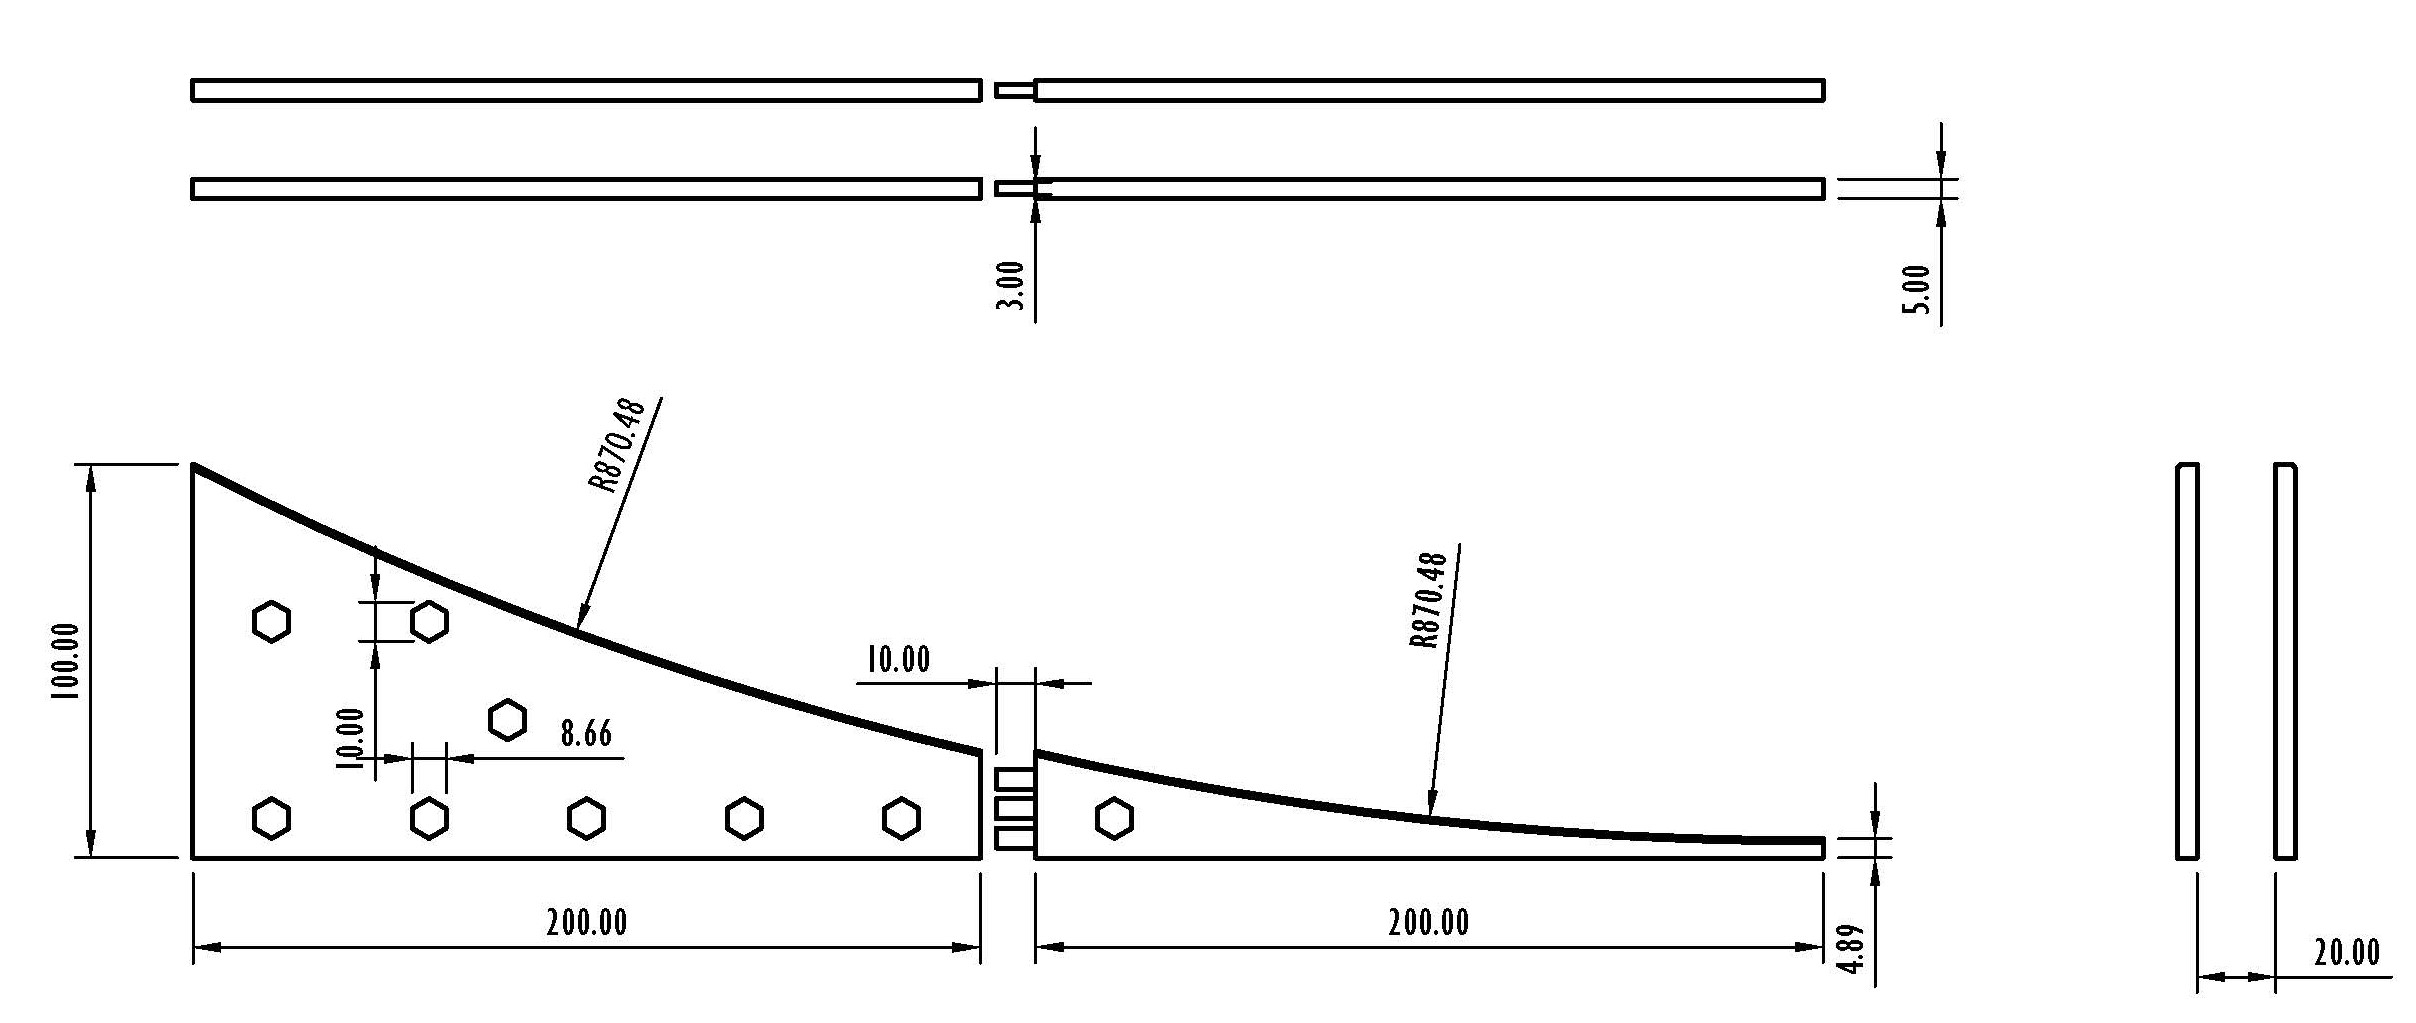
\includegraphics[width=0.99\textwidth]{images/rampedraw2.jpg}
  \caption[Technische Zeichnung der Beschleunigereinheit]{Zu sehen ist eine technische Zeichnung der geplanten Beschleunigereinheit, die auf einen 3D-Druck ausgelegt ist, jedoch mit leichten Anpassungen auch auf einer \textsw{CNC-Fräse} aus einer Stahlplatte mit Dicke $d=\SI{5}{\milli\metre}$ gefertigt werden kann. Die Rampe besitzt durch  die Aussparung eines Kreisbogens mit Radius $r=\SI{900}{\milli\metre}$ von $\SI{267.2}{\degree}$ bis $\SI{270}{\degree}$ einen nahezu waagerechten Auslauf.}
  \label{fig:rampedraw}
  \vspace{-0pt}
\end{figure}

\noindent Die Schiene dieser Rampe ist zweigeteilt und hat jeweils eine Aussägung in Form eines Kreisbogens mit Radius $r=\SI{900}{\milli\metre}$ von $\SI{267.2}{\degree}$ bis $\SI{270}{\degree}$. Die sechseckigen Aussparungen sind für die Aufnahme von Muttern gedacht, die mittels \textit{WIG}-Schweißen (\textsw{W}olfram-\textsw{I}nert\textsw{g}as) befestigt werden können. Oben links an der Vorderseite wird eine rechtsdrehende, auf der Rückseite eine linksdrehende Mutter verwendet. Die Mutterorientierung muss sich immer abwechseln, damit angebrachte Zahnräder gleichgerichtet drehen. Durch die mechanische Werkstatt werden Gewindestangen geschnitten, die jeweils hälftig aus Links- und Rechtsgewinde bestehen. 

An diese Gewindestangen werden einseitig die Zahnräder mit \textit{Madenschrauben} befestigt. Somit kann die Rampe bei Drehung des linken oberen Zahnrades nach rechts zusammen und bei Drehung nach links auseinander gefahren werden.

Da die Rampe möglichst schnell funktionsfähig sein muss, und gewisse Probleme mit dem vorhandenem 3D-Drucker bestehen, wird die Rampe aus Sperrholz selbst angefertigt, wie auf Foto \ref{fig:rampenschliff1} zu sehen ist. Die Aussparungen für die Muttern --- welche anschließend eingeklebt werden --- entstehen durch Bearbeitung mit einem Stechbeitel der Eisenbreite $\SI{3}{\milli\metre}$. Die Muttern werden anschließend eingeklebt und die beiden Rampensegmente mit den Gewindestangen verbunden.

%% Autor: Björn Ritterbecks 
%% Letzte Aenderung: 15.06.2016 
\thisfloatsetup{%
  capbesidewidth=\marginparwidth}
\begin{figure}[htbp]
\centering
%\sansmath
 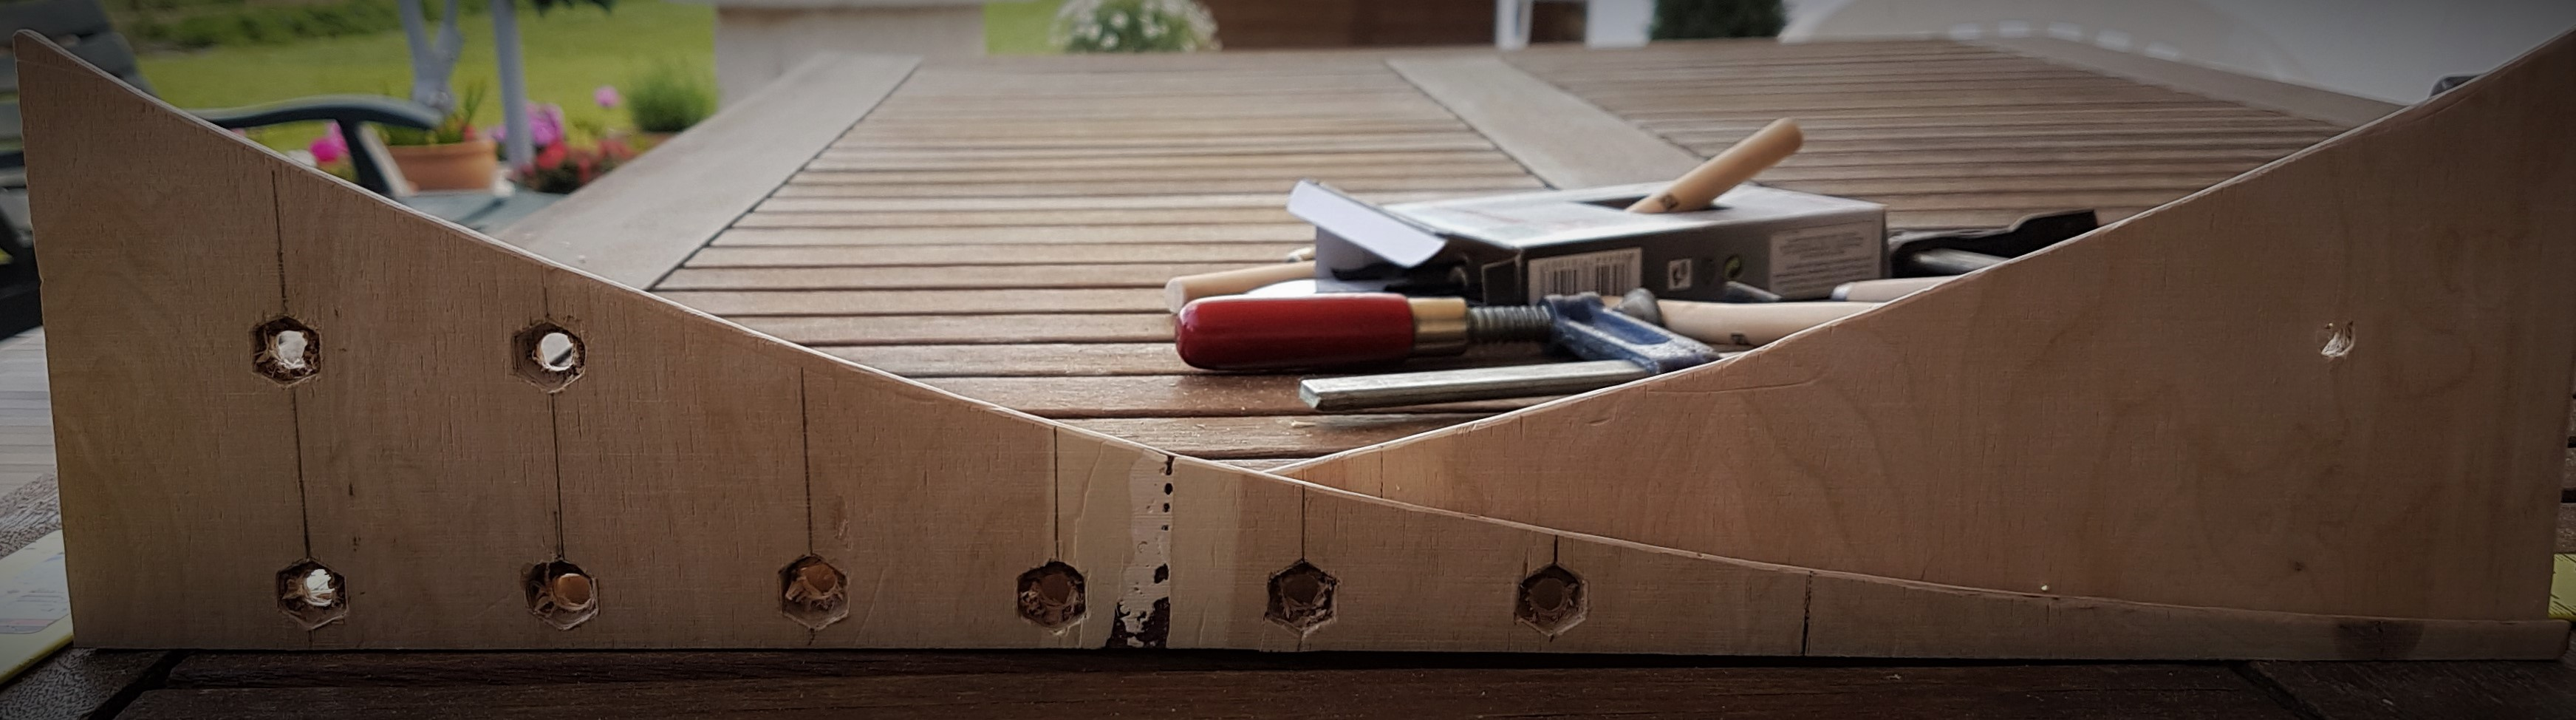
\includegraphics[width=0.99\textwidth]{images/rampenschliff1.jpg}
  \caption[Gesägte und gehobelte Rampensegmente]{Seitenansicht der gebauten Rampensegmente. Mittels eines nicht dehnbaren Fadens, Winkeln und einigen Schraubzwingen wird die Form angezeichnet und anschließend auf der Abfallseite ausgesägt. Die Annäherung an die endgültige Form erfolgt durch einen fein eingestellten Schweifhobel. Nach dem Durchbohren mit einem $\SI{6}{\milli\metre}$ Bohrer werden die Aussparungen für die Mutteraufnahme mit einem Stechbeitel gefertigt.}
  \label{fig:rampenschliff1}
  \vspace{-0pt}
\end{figure}

\noindent Bei der Arbeit mit Holz ist eine Genauigkeit von einem halben Millimeter bereits ordentlich, die von der Werkstatt --- aus Aluminium --- geschnittenen Gewinde verzeihen jedoch kaum ein Abweichen von der Parallelität der Muttern. Da Aluminium ein weicher Werkstoff mit hohem Abrieb ist, sind die Gewinde schnell zerstört. Bei einem erneuten Bau sollten sie demnach zumindest aus Messing gefertigt werden.

%% Autor: Björn Ritterbecks 
%% Letzte Aenderung: 15.06.2016 
\thisfloatsetup{%
  capbesidewidth=\marginparwidth}
\begin{figure}[htbp]
\vspace*{0.2cm}
\centering
%\sansmath
 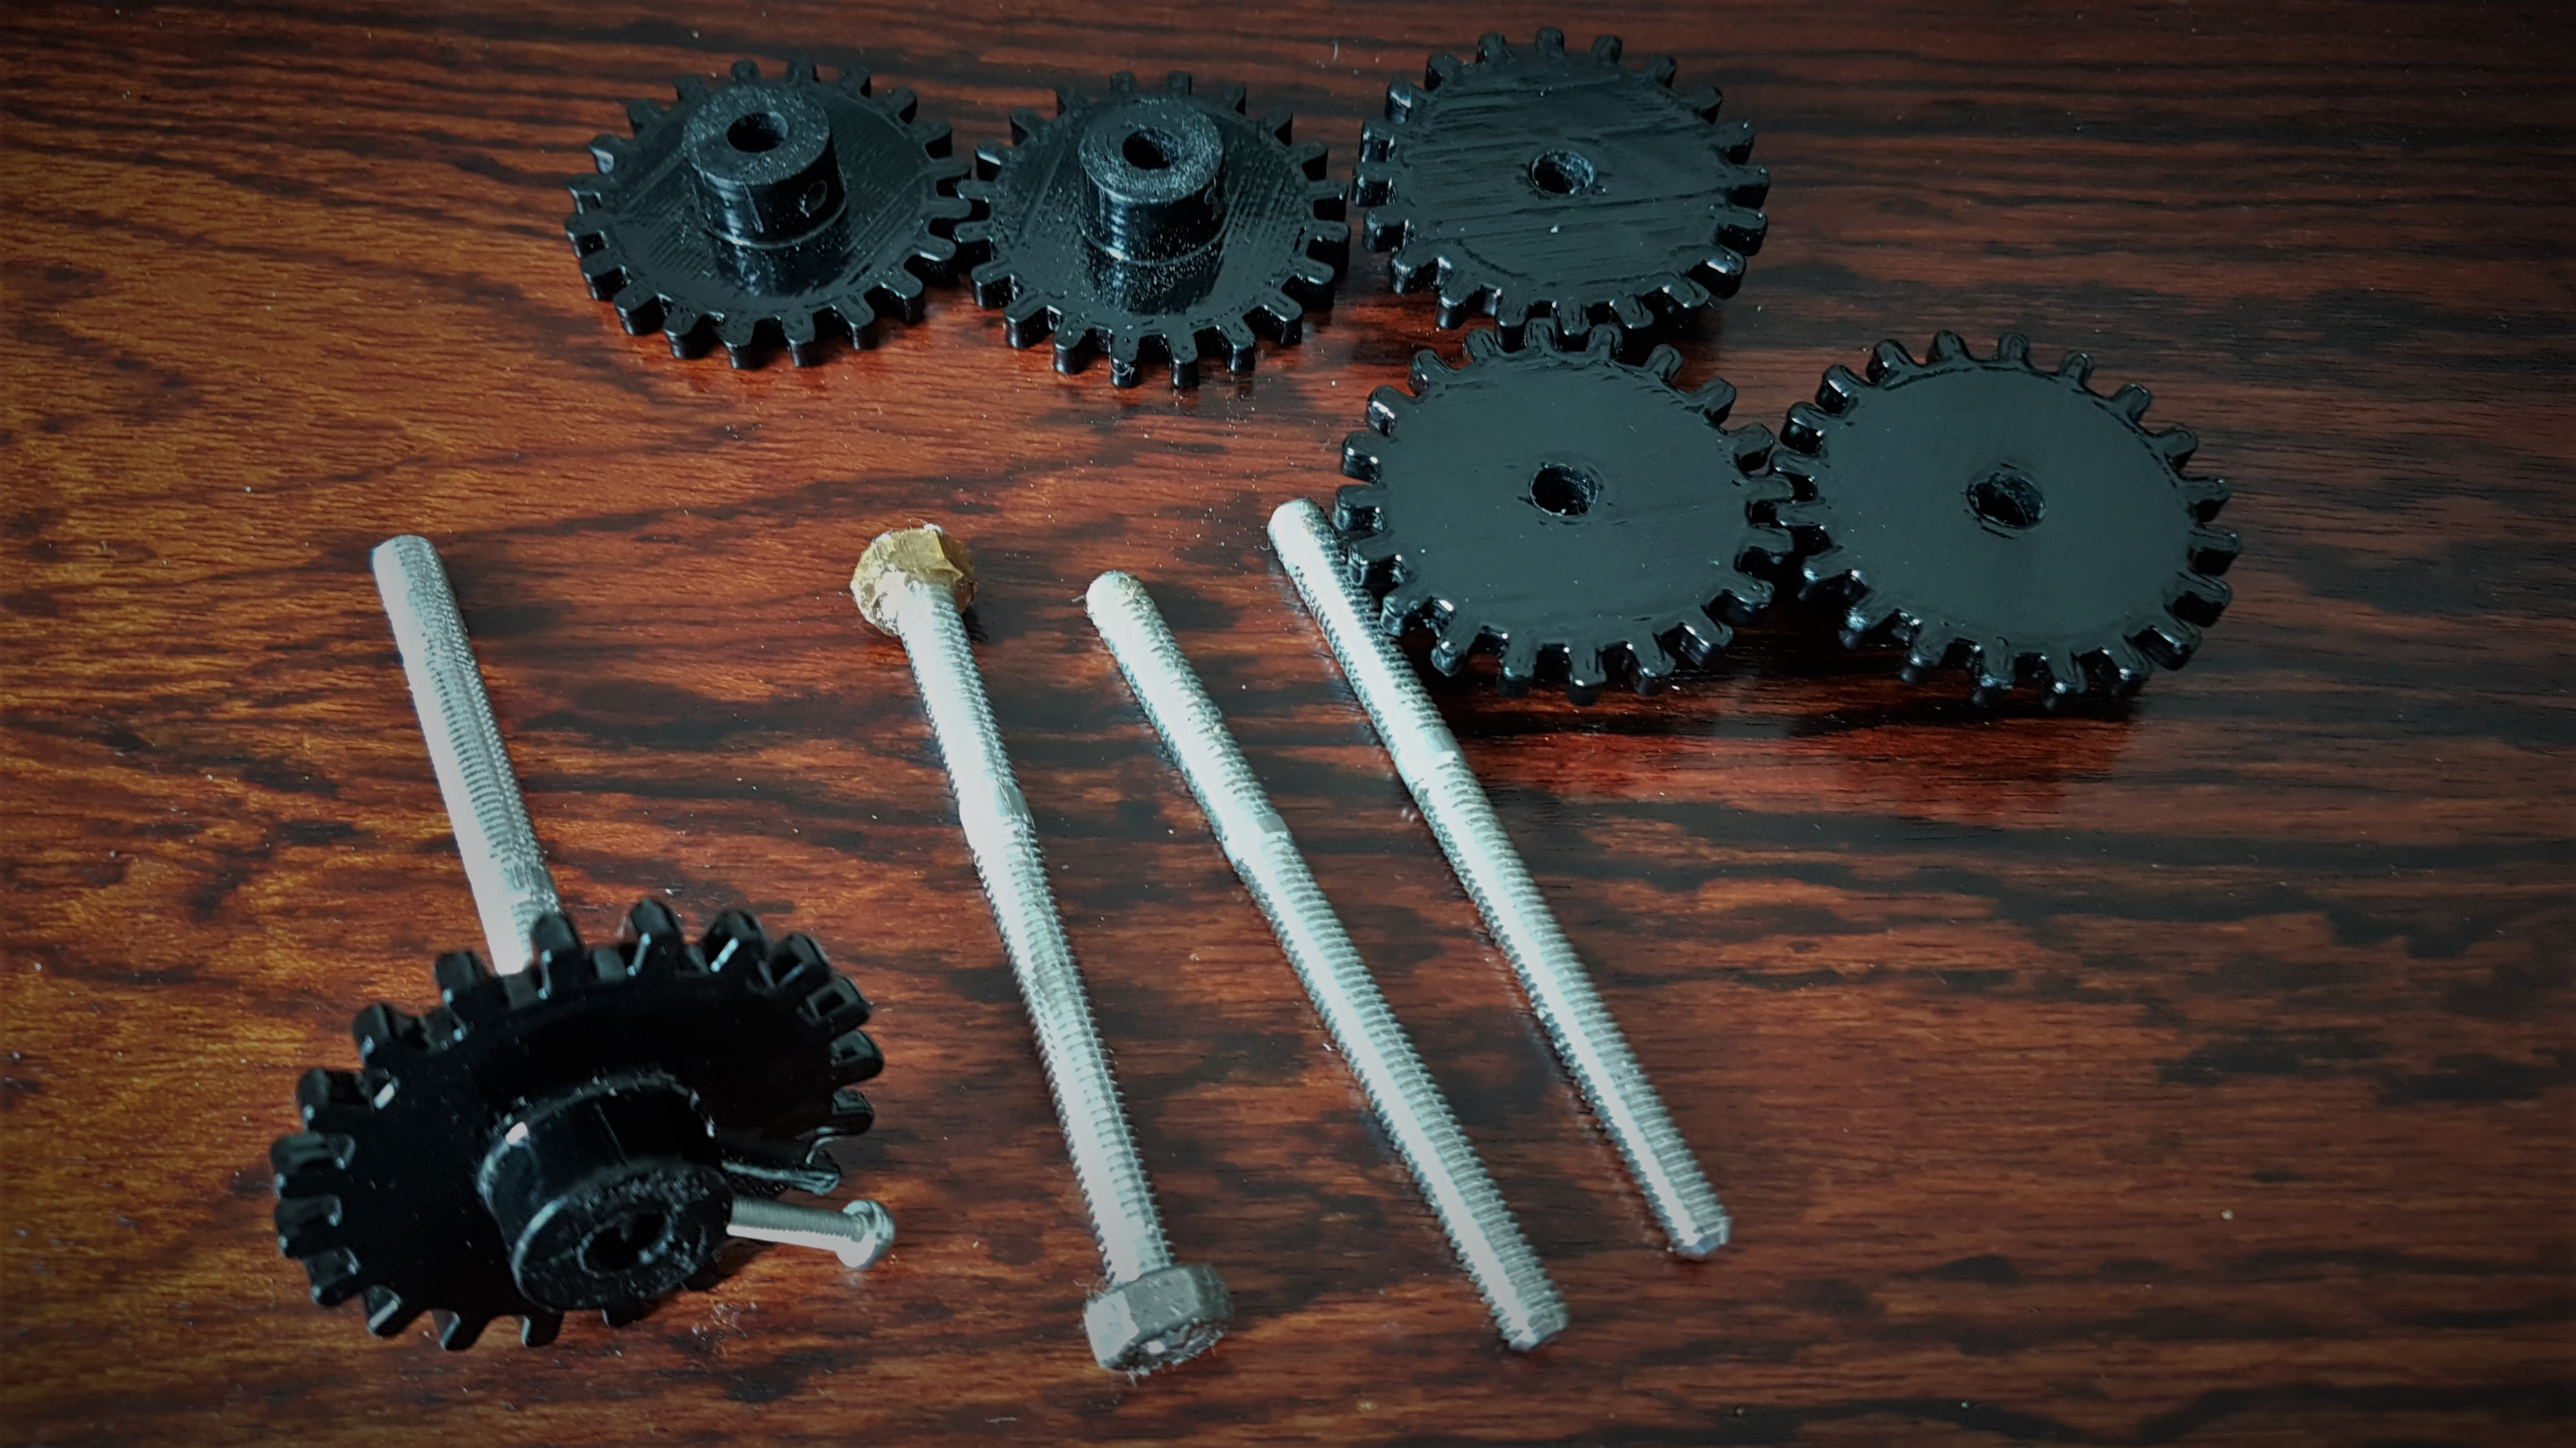
\includegraphics[width=0.99\textwidth]{images/toothpaste.jpg}
  \caption[Fotografie der Zahnräder und Gewinde]{Fotografische Abbildung der Zahnräder und Gewinde nach dem Ausbau. Bei Versuchen vor dem Einkleben der Muttern haben beide Komponenten gut funktioniert, wurden jedoch bei der Arretierung an der Beschleunigereinheit in ihrer Funktionalität zerstört (unter anderem durch Kleberückstände und mangelhafte Parallelität).}
  \label{fig:toothpaste}
  \vspace{-0pt}
\end{figure}

Die Zahnräder werden mit dem 3D-Drucker bei maximaler Dichte aus \textit{ABS} (\textsw{A}crylnitril-\textsw{B}utadien-\textsw{S}tyrol) gedruckt, um das Schneiden eines Gewindes für die Madenschrauben zu ermöglichen. Anschließend werden Ungenauigkeiten des Druckergebnisses in einem \textit{Aceton-Dampfbad} bereinigt. Sowohl die Zahnräder als auch die Gewinde sind in Abbildung \ref{fig:toothpaste} dargestellt. Problematisch ist jedoch, dass die Gewinde schon bei recht geringem Zug ausreißen, da der verwendete Kunststoff nicht hart genug ist.

Trotz der Unwägsamkeiten wird die Rampe mit der Vorrichtung aus Abbildung \ref{fig:rampfenschliff2} an den Experimentiertisch geschraubt. Eine Kugel wird auf das waagerechte Rampensegment gelegt, welches so auseinander-/zusammengeschoben wird, bis die Kugel die Tischplatte leicht berührt. Der Aufbau ist trotz der fehlenden Automatisierung praktikabel, wenn beide Gleise einzeln justiert und mit Gewindestangen fixiert werden.

%% Autor: Björn Ritterbecks 
%% Letzte Aenderung: 15.06.2016 
\thisfloatsetup{%
  capbesidewidth=\marginparwidth}
\begin{figure}[htbp]
\vspace*{0.2cm}
\centering
%\sansmath
 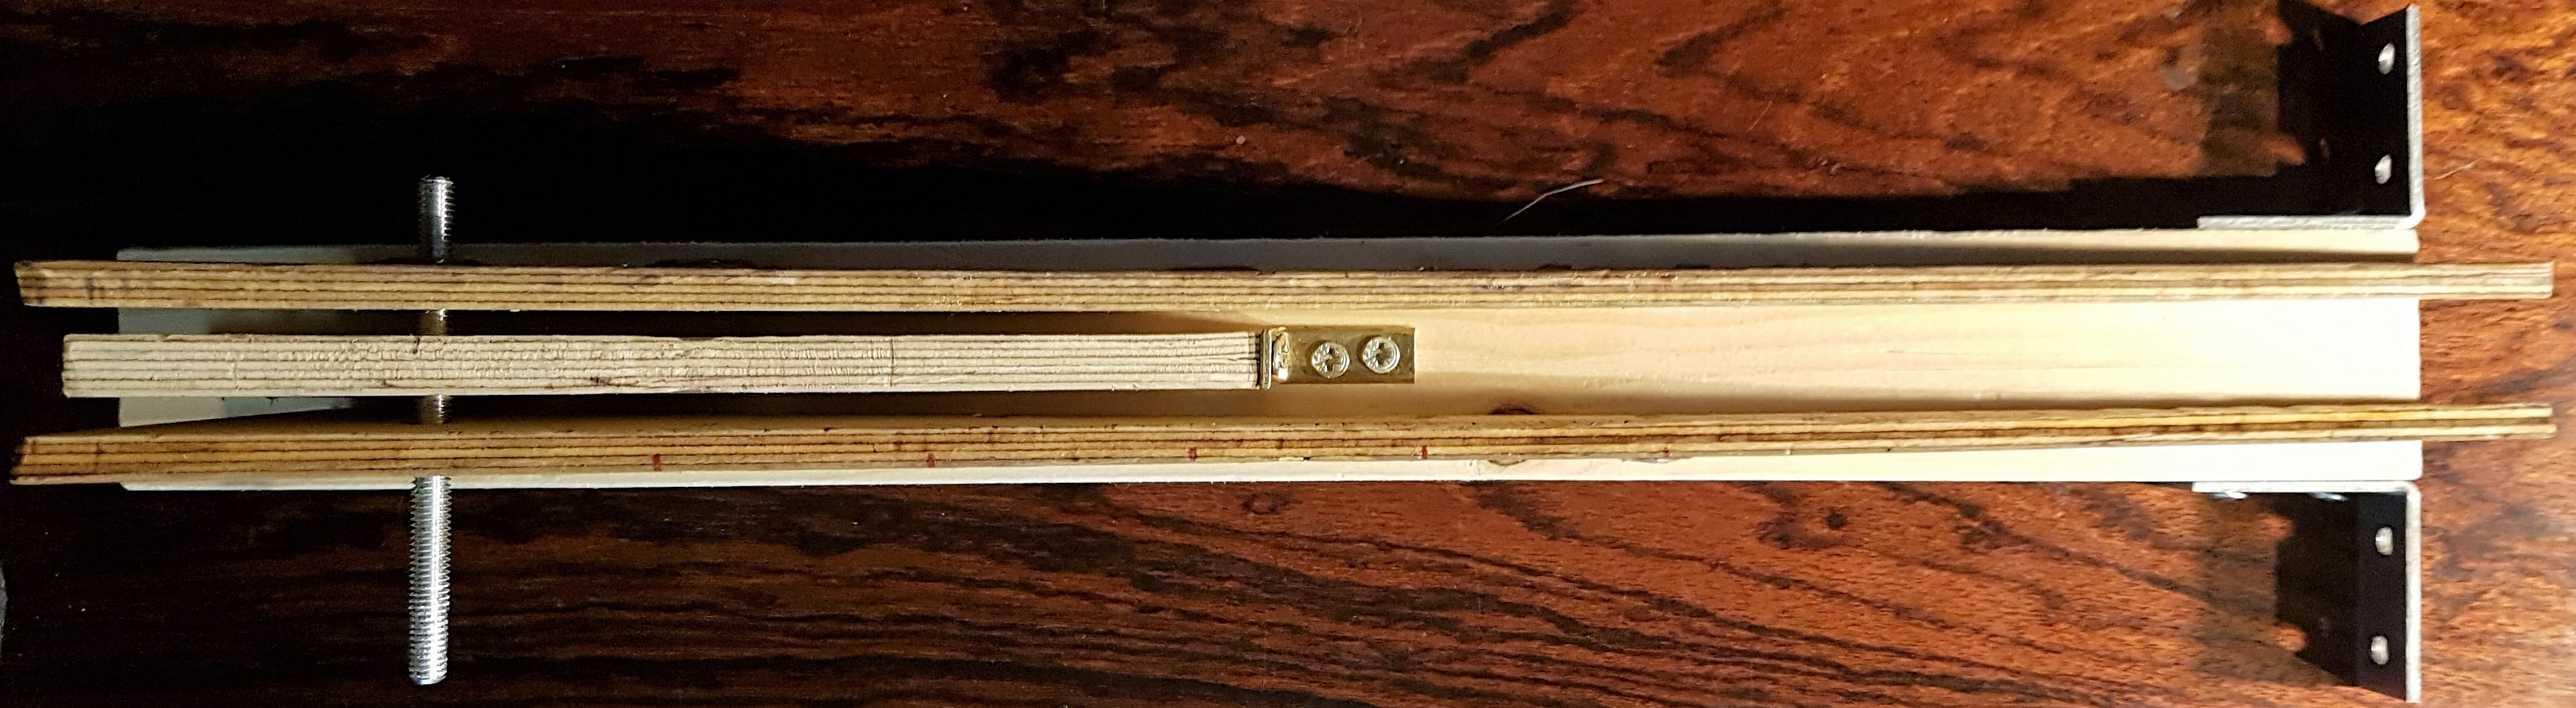
\includegraphics[width=0.99\textwidth]{images/rrampe1.jpg}
  \caption[Draufsicht der gebauten Rampe]{Die Startrampe ist auf ein Brett montiert, welches wiederum mit zwei Winkeln an den Experimentiertisch angeschraubt werden kann. Durch die Anordnung auf einem schmalen Brett lässt sich zum Einen die Rechtwinkligkeit gut überprüfen, zum Anderen erlaubt es den Zahnrädern in vertikaler Richtung bis unterhalb der Tischplatte zu reichen. Auf der linken Seite mittig ist ein Holzblock mit Ausbohrungen, durch welche die Gewindestangen zur Zentrierung gesteckt hätten werden sollen.}
  \label{fig:rampfenschliff2}
  \vspace{-0pt}
\end{figure}

\section{Kugeln}
\label{sec:balls}

Wie in den Analogiebetrachtungen bereits erwähnt, gibt es zwei Anforderungen an die Ionenanalogie: Es werden Kugeln benötigt, die in ihrer Größe und Dichte unterscheidbar sind. Um die Analogie $\sfrac{q}{m}\widehat{=}\sfrac{A_\mathrm{proj}}{m}$ weiter zu verbessern, soll die Quantelung der Ladung berücksichtigt werden, indem $A_{\mathrm{proj},i}=i\cdot A_{\mathrm{proj},0}$ gilt. Dies wäre zum Beispiel bei den Kugelradien $\SI{10}{\milli\metre}$, $\SI{14}{\milli\metre}$, $\SI{17}{\milli\metre}$ und $\SI{20}{\milli\metre}$ näherungsweise erfüllt.

Da frei verfügbare Kugeln meistens in einer Schrittweite von $\SI{5}{\milli\metre}$ zu kaufen sind, entfällt diese Möglichkeit. Eine Anfrage an Produzenten von Präzisionskugeln verschiedener Werkstoffe ergab für einen Satz von 4 Kugelradien und 4 Werkstoffen gut unterscheidbarer Dichte, d.\,h. 160 Kugeln, einen Preis über $1\,000,-\euro$. 

Eine weitere Möglichkeit, diese Forderungen zu erfüllen, wird darin gesehen, einen 3D-Drucker zu verwenden und die Füllung zwar homogen, jedoch zwischen den einzelnen Kugelarten unterscheidbar zu gestalten (bei 3D-Druckern besteht die Möglichkeit, die Dichte des Füllmaterials zu bestimmen). 

%% Autor: Björn Ritterbecks 
%% Letzte Aenderung: 15.06.2016 
\thisfloatsetup{%
  capbesidewidth=\marginparwidth}
\begin{figure}[htbp]
\centering
%\sansmath
 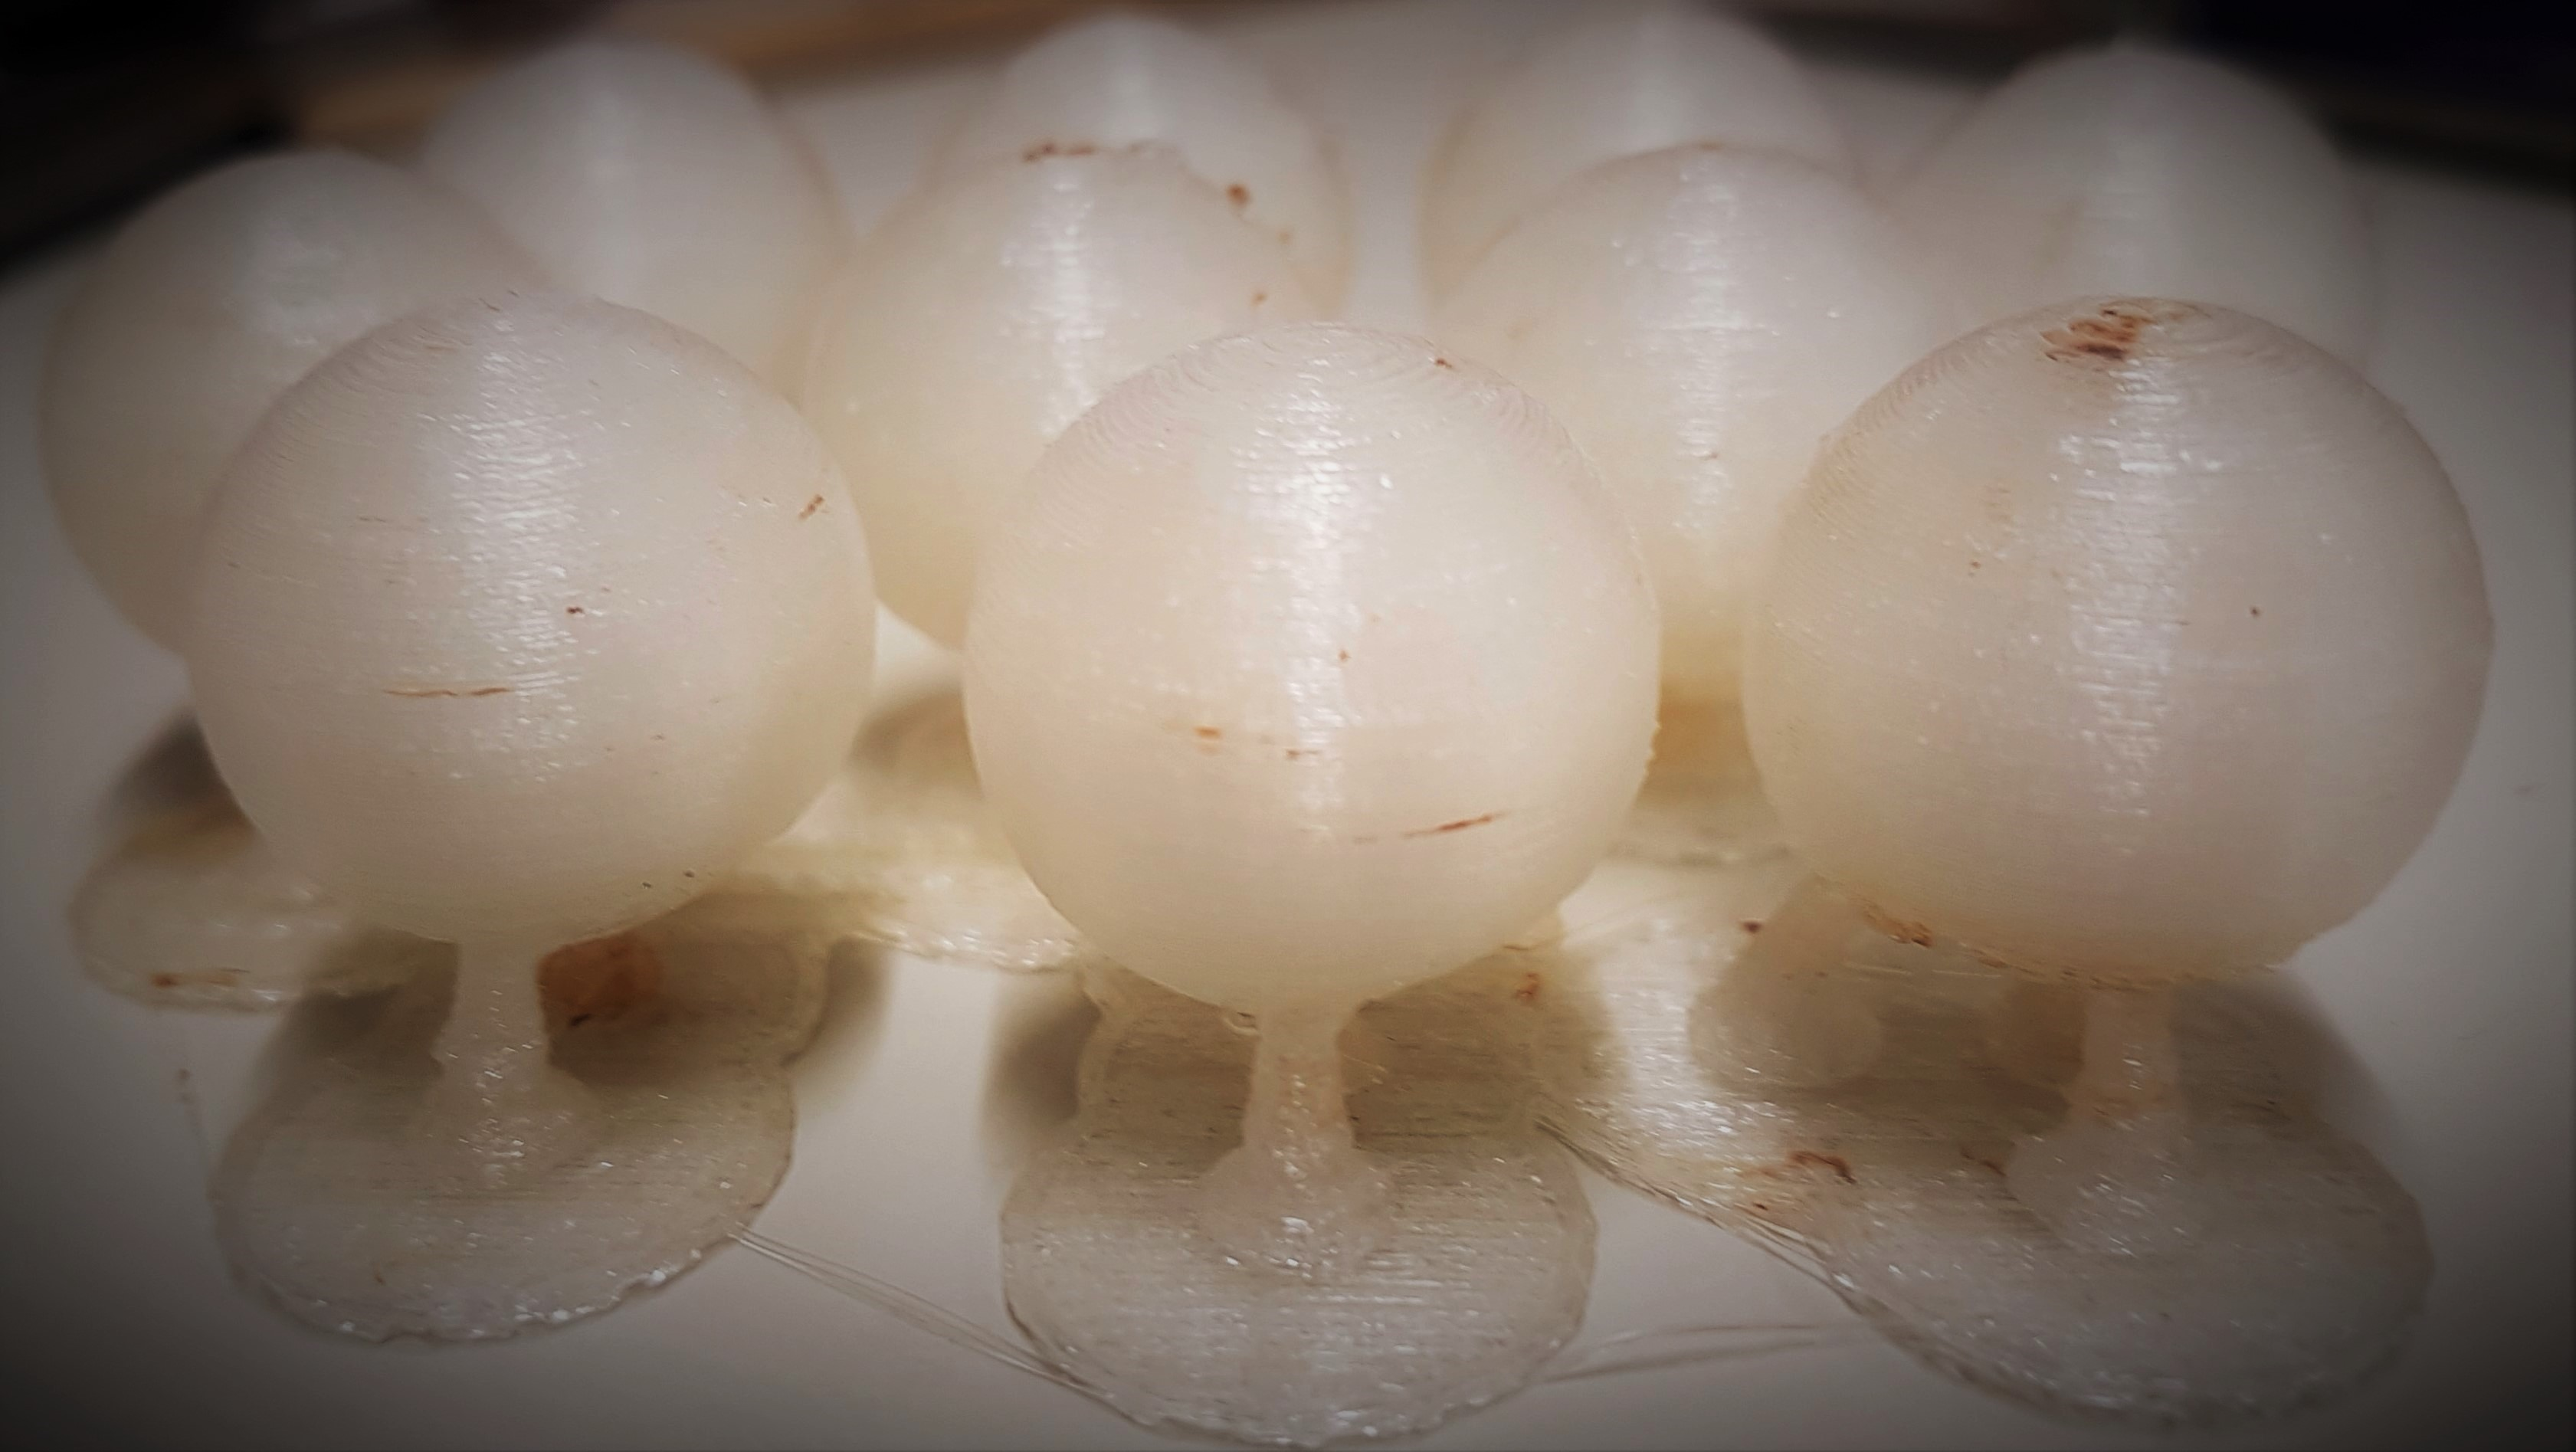
\includegraphics[width=0.99\textwidth]{images/gedrucktekugeln2.jpg}
  \caption[3D-gedruckte Kugeln]{Zu sehen ist der erste Versuch für 3D-gedruckte Kugeln auf einem Stützensystem.}
  \label{fig:gedrucktekugeln2}
  \vspace{-0pt}
\end{figure}

\noindent Nach einem Probedruck von zwei Kugelhälften, die jeweils auf der Flachen Seite erstellt worden sind, wird der erste Satz von 10 Kugeln mit maximaler Dichte und einem Radius von $\SI{10.0}{\milli\metre}$ auf einem Stelzengeflecht gedruckt (siehe Abb. \ref{fig:gedrucktekugeln2}). Dieser Druck ergibt leider kein gutes Resultat, da die Unterseiten abgeflacht und somit die Kugeln nicht Rotationssymmetrisch sind. Bei dem Versuch, jeweils zwei Kugelhälften mit Aceton zusammenzukleben, fiel jedoch, wie auf Foto \ref{fig:fail} zu sehen ist, auf, dass trotz maximaler Druckdichte die Kugelschale wesentlich dichter gedruckt ist, als das Innenleben, und somit keine homogene Massenverteilung gewährleistet wird. 

%% Autor: Björn Ritterbecks 
%% Letzte Aenderung: 15.06.2016 
\thisfloatsetup{%
  capbesidewidth=\marginparwidth}
\begin{figure}[htbp]
\vspace*{0.2cm}
\centering
%\sansmath
 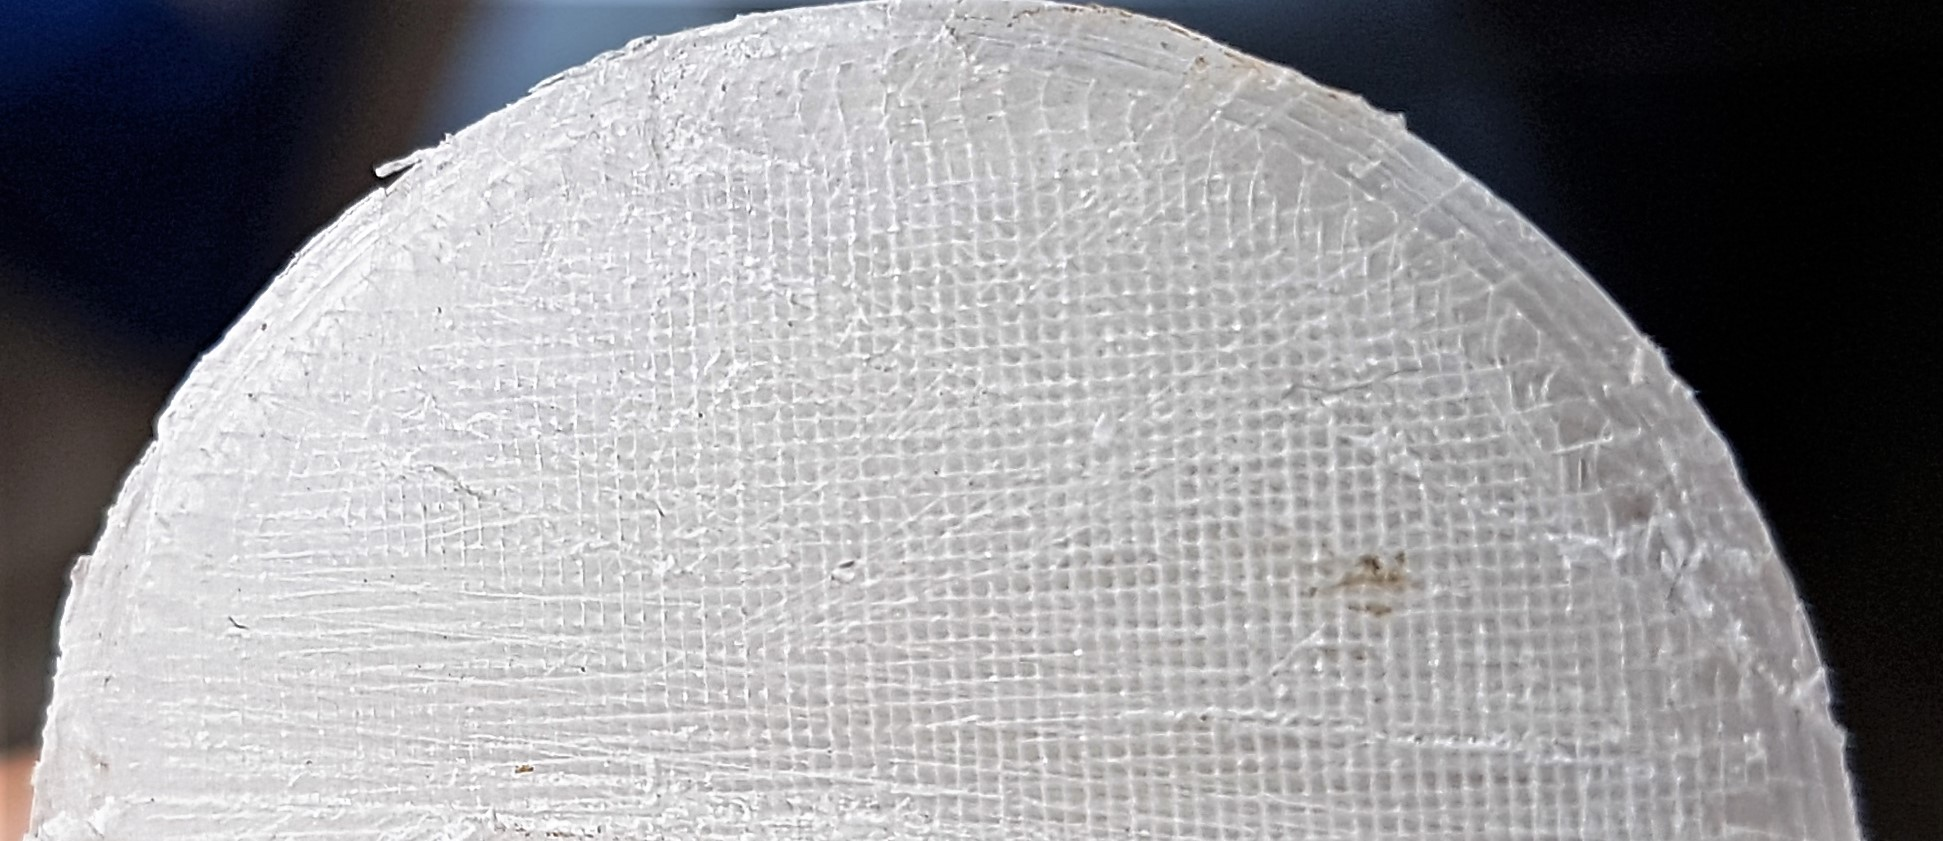
\includegraphics[width=0.99\textwidth]{images/fail.jpg}
  \caption[Aufgeschnittene Kugel aus dem 3D-Drucker]{Auf diesem Foto einer aufgeschnittenen, 3D-gedruckten Kugel ist gut zu erkennen, dass die Wandschicht der Kugel mit einer höheren Dichte gedruckt wurde.}
  \label{fig:fail}
  \vspace{-0pt}
\end{figure}

\noindent Um dennoch die restlichen Komponenten zufriedenstellend untersuchen zu können, wurden im Anschluss Holzkugeln aus dem Bastelbedarf und Glaskugeln (einfache Murmeln) gekauft. 

\section{Schiefe Ebene}

Die erste Hälfte der Experimentierplatte zu einer schiefen Ebene zu machen, während die zweite Hälfte in der Waage bleibt, wird realisiert, indem beide Teilplatten separat auf jeweils vier Standfüße, die unabhängig voneinander einstellbar sind, montiert werden, so dass beim Aneinanderschieben der beiden Platten die rechte waagerecht ist und die linke Platte an der Vorderkante einige Millimeter höher und an der Hinterkante dieselbe Distanz tiefer, jedoch in $x$-Richtung ebenfalls in der Waage liegt.

Die Fixierung der beiden Platten und damit auch die Möglichkeit eines Transportes wird durch gehobelte Bretter umgesetzt, bei denen jeweils eine Hälfte um einige Zehntelmillimeter abgeschrägt wird, während die andere Hälfte um die festgelegte Anzahl an Millimetern abgeschabt wird (siehe Foto \ref{fig:brettvorderplatte}). Auf diese Weise kann die Neigung der schiefen Ebene festgelegt werden. Beispielsweise bei einer Plattenbreite von $\SI{40}{\centi\metre}$ führen jeweils $\SI{2}{\milli\metre}$ an der Vorder- und Hinterkante zu einer Neigung von $1:100$.

%% Autor: Björn Ritterbecks 
%% Letzte Aenderung: 15.06.2016 
\thisfloatsetup{%
  capbesidewidth=\marginparwidth}
\begin{figure}[htbp]
\vspace*{0.2cm}
\centering
%\sansmath
 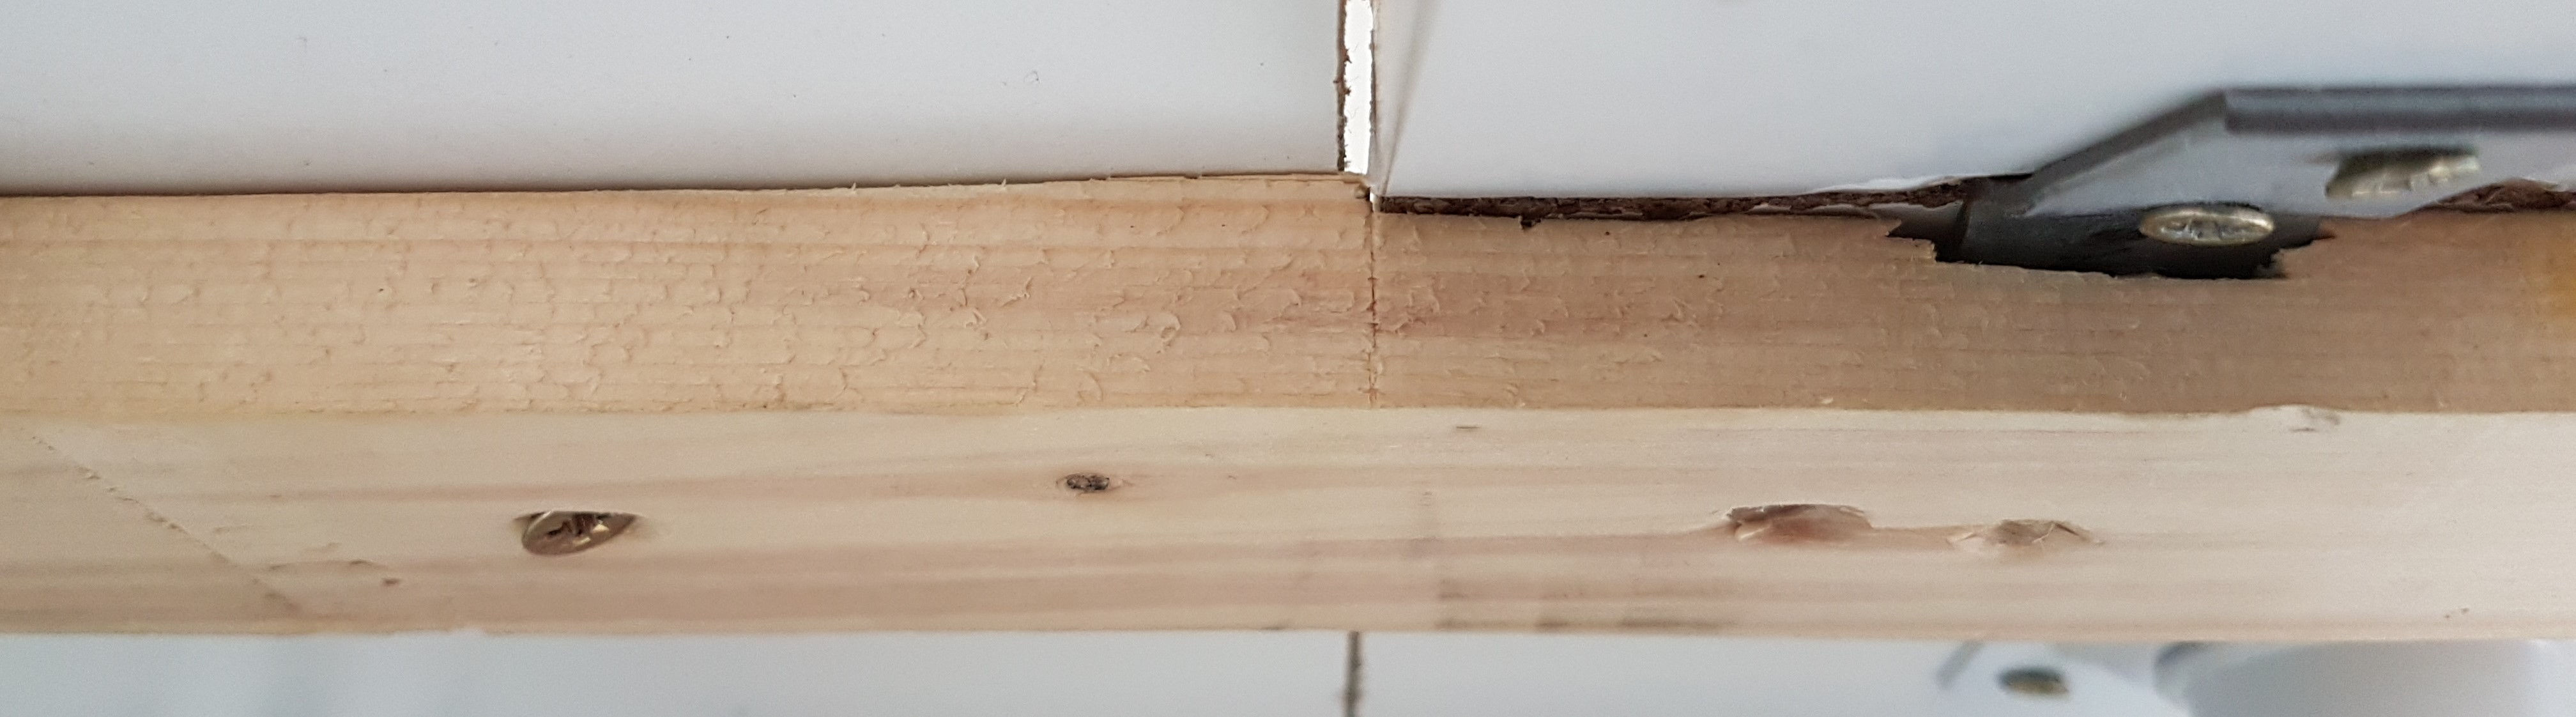
\includegraphics[width=0.99\textwidth]{images/brettvorderplatte.jpg}
  \caption[Übergangsbereich schiefe Ebene]{Zu sehen ist der Übergangsbereich zwischen schiefer Ebene und waagerechter Platte, der jeweils an der Vorder- und Hinterkante mit einem passend abgehobeltem Brett fixiert wird. Der um $\SI{15}{\degree}$ geneigte Plattenteil ist erst nach den Messungen hinzugefügt worden, um der Winkelaufspaltung der Kugeln genüge zu tun (d.\,h., dass die Breiten der einzelnen Detektoren nach rechts hin zunehmen müssen.)}
  \label{fig:brettvorderplatte}
  \vspace{-0pt}
\end{figure}

\noindent Im Übergangsbereich der Platten wird --- wie bei \textcite{Schilling1987} --- Isolierband geklebt, damit die Kugeln den Höhenunterschied möglichst ohne Aufprallen/Springen überwinden können. Die Festlegung der Plattenneigung erfolgt über Berechnungen in \textit{Excel} und beträgt bei den Messungen ca. $1:35$, da eine möglichst große Auslenkung auf der schiefen Ebene gewünscht ist. Wie die Messungen zeigen werden, sollte jedoch für den endgültigen Aufbau ein geringeres Gefälle gewählt werden. Der Baustand während der Probemessungen kann in Abbildung \ref{fig:aufbau1} betrachtet werden.

%% Autor: Björn Ritterbecks 
%% Letzte Aenderung: 15.06.2016 
\thisfloatsetup{%
  capbesidewidth=\marginparwidth}
\begin{figure}[htbp]
\vspace*{0.2cm}
\centering
%\sansmath
 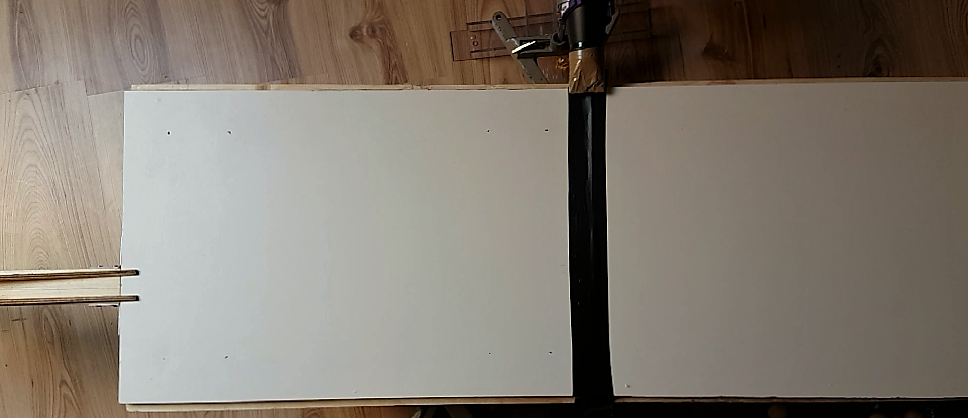
\includegraphics[width=0.99\textwidth]{images/Aufbau.png}
  \caption[Versuchsaufbau ohne Detektoren]{Fotografie des Versuchsaufbaus ohne Detektoren. Bei der linken Platte handelt es sich um die schiefe Ebene. Das Gebläse wirkt mit der höchsten Kraft im Übergangsbereich der beiden Platten. Durch die Aufhängung mit Winkeln kann die Rampe auch näher am Gebläse positioniert werden.}
  \label{fig:aufbau1}
  \vspace{-0pt}
\end{figure}

\section{Detektoren}



Wie bereits von \textsc{Mais} angemerkt, geschieht die Aufspaltung der analysierten Teilchen (Kugeln) radialsymmetrisch um den Punkt der größten Krafteinwirkung. Auch bei einem geschwindigkeitsfokussierenden Aufbau ändert sich nichts an diesem Prinzip, wobei jedoch zwischen den langsamsten und schnellsten Kugeln ein mittlerer Auslenkwinkel bestimmt werden muss. Aufgrund der Unzulänglichkeiten der verwendeten Holz- und Glaskugeln ist diese Kalibrierung noch nicht erfolgen.
An dieser Stelle wird dennoch der Versuch unternommen, die Grundlagen einer praktischen Umsetzung zu beschreiben.
%% Autor: Björn Ritterbecks 
%% Letzte Aenderung: 15.06.2016 
\begin{marginfigure}
\vspace*{0.2cm}
\centering
%\sansmath
 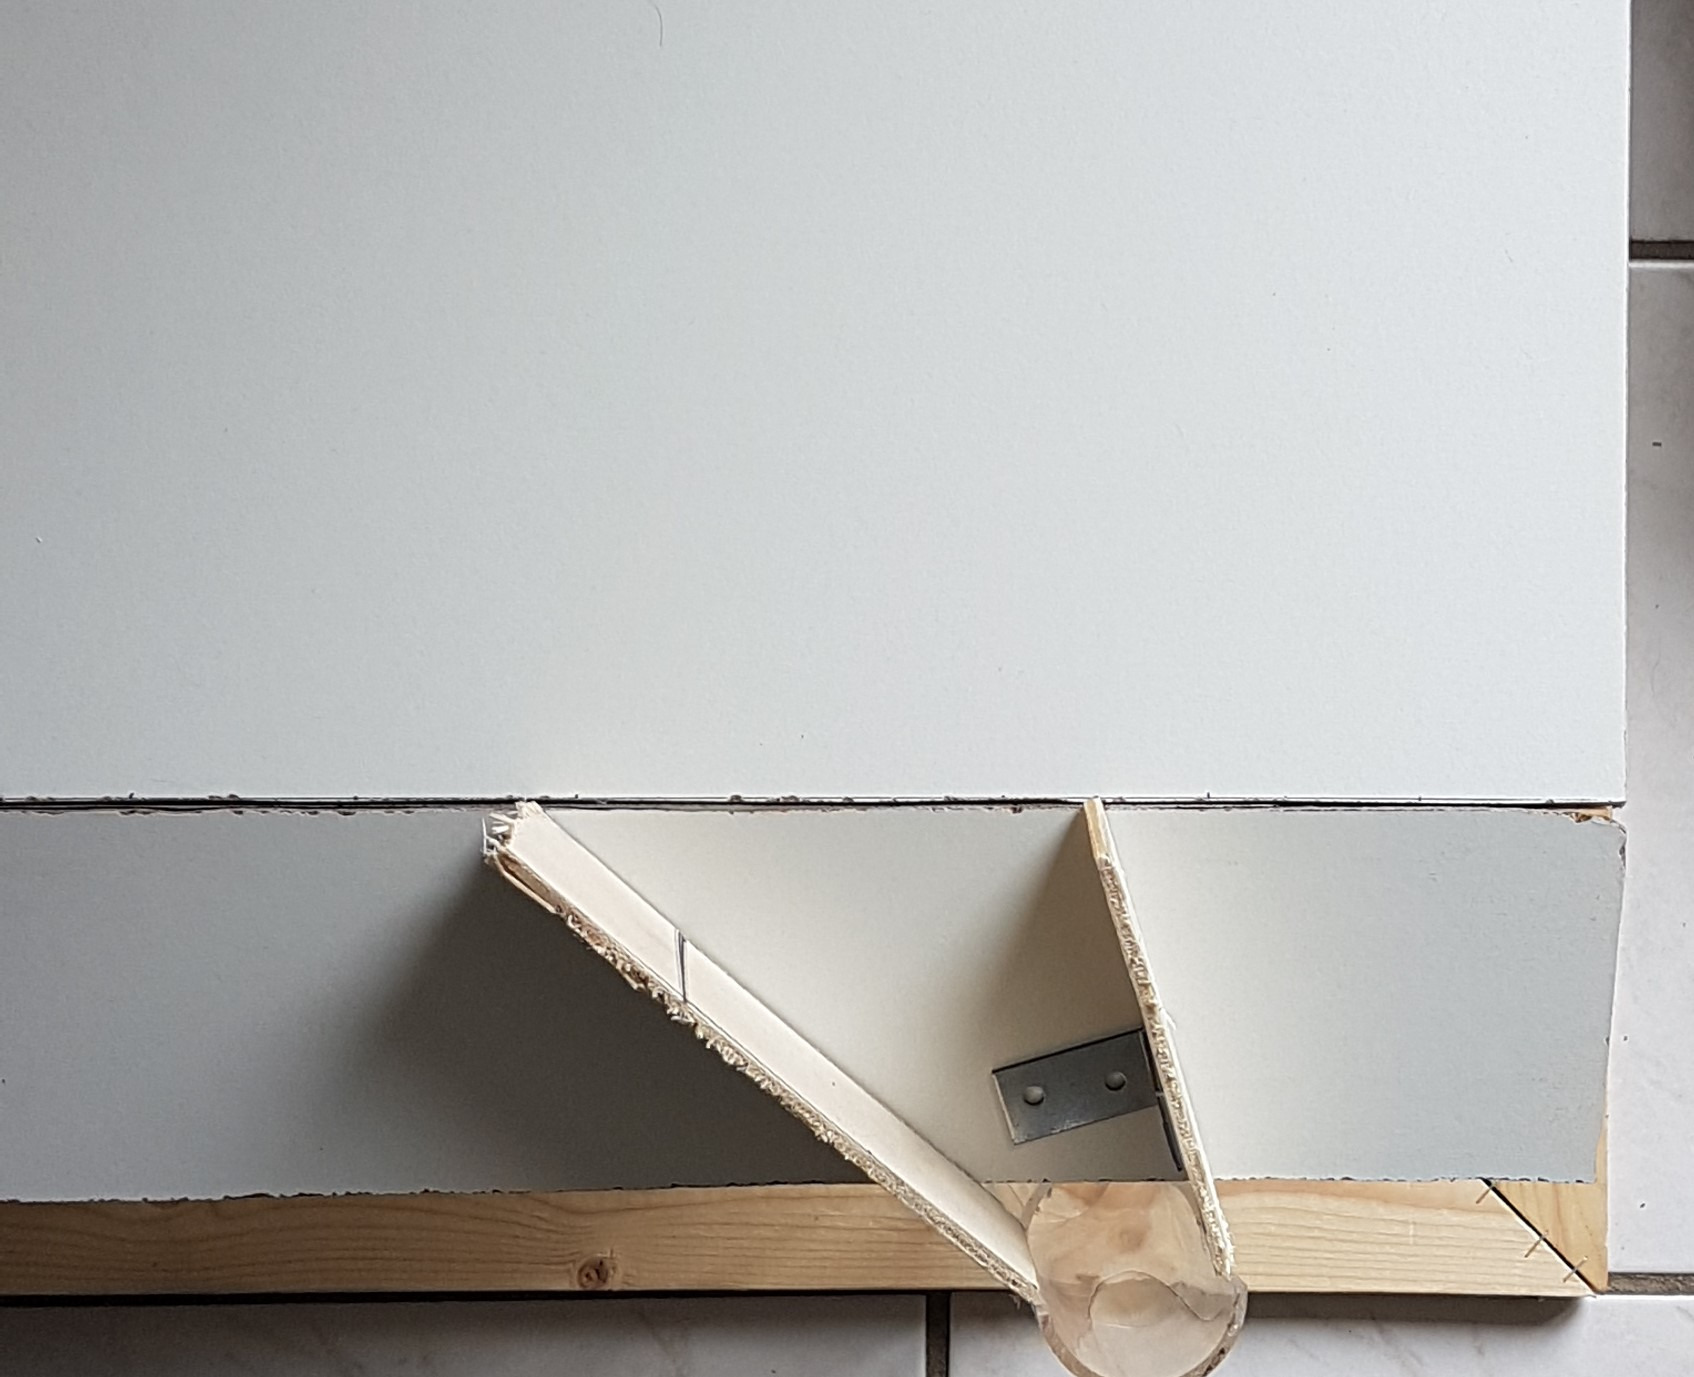
\includegraphics[width=0.99\marginparwidth]{images/istregistriert.jpg}
  \caption[Detektionsnsprinzip]{Vorschlag einer Detektoranordnung: Je geringer der Detektionswinkel ist, desto größer muss die Breite der einzelnen Detektoren sein. Damit selbst bei den größten Detektoren alle Kugeln in die Röhren rollen können, ist der rechte Teil der Platte um $\SI{15}{\degree}$ geneigt. Ein letzter Detektor wird am rechten Ende angebracht.}
  \label{fig:istregisrtiert}
  \vspace{-0pt}
\end{marginfigure}

Bei dem Aufbau nach \textcite{Schilling1987} sind die Detektoren in einem festen Abstand $b$ zueinander angebracht. Dies führt allerdings --- bereits bei oberflächlicher Betrachtung dazu, dass ein Teil der weiter rechts liegenden Detektoren nur noch einige $\SI{E-1}{\degree}$ detektieren kann. Die waagerechte Platte ist ca. $\SI{65}{\centi\metre}$ lang, die schiefe Ebene etwa $\SI{55}{\centi\metre}$ (vgl. \ref{fig:mnu}). Somit entspricht die Ablenkung im Gravitationsfeld bei einer Starthöhe von $\SI{2}{\centi\metre}$ bis $\SI{8}{\centi\metre}$ zwischen $\SI{5}{\centi\metre}$ und $\SI{1}{\centi\metre}$. Nimmt man an, dass bei \textsc{Schilling} jeder Detektor eine Breite von $\SI{9}{\centi\metre}$ hat, so würde der letzte Detektor in einem Winkel zwischen $\SI{5.5}{\degree}$ und $\SI{4.7}{\degree}$ getroffen werden (bei den langsamsten Kugeln) und zwischen $\SI{1.2}{\degree}$ und $\SI{1.0}{\degree}$ bei den schnellsten, jedoch der erste Detektor bei den langsamen Kugeln im Bereich von $\SI{90}{\degree}$ bis $\SI{39}{\degree}$.

Diese qualitativen Rechnungen gelten natürlich nur, wenn die Detektion auf der Fokussierungsachse erfolgen soll. Da die Impulsänderung $\Delta p$ linear mit dem Gewicht skaliert, wird schnell klar, dass im Bereich hoher Kugeldichten der Analysator ein hohes Auflösungsvermögen hätte, wenn die Analysatorlänge stark ausgedehnt werden würde. 

Damit wird eine L-förmige Detektoranordnung vorgeschlagen, die auch Massen mit einem Registrierwinkel nahe $\SI{1}{\degree}$ wahrnehmen kann. Die Konzeption ist auf dem Foto \ref{fig:istregisrtiert} zu sehen: Je schwerer die Massen sind, desto weiter rechts werden sie detektiert und umso geringer ist der Auftreffwinkel. Somit bräuchten die linken Detektoren keine Breitenanpassung, sondern erst diejenigen weiter rechts. Da die Kugeln bei einem geringen Auftreffwinkel an den Begrenzungen der Detektoren hängen bleiben könnten, wird die waagerechte Platte bei $y=0$ abgetrennt und mit einer Neigung von $\SI{15}{\degree}$ erneut angeschraubt. Dieses Prinzip ist bereits 1970 in ähnlicher Form von der \textsc{Nuffield Foundation} verwendet worden (vgl. Abb. \ref{fig:nuffsaid}).



\chapter{Gültigkeit}
\label{kap:5}
\bookmarksetupnext{level=subsubsection}
\chapterinfo{Die entscheidenden Versuchsparameter werden durch selbstgebaute Apparaturen gemessen und mit den theoretischen Erwartungen verglichen, um aus der Schnittmenge ein mathematisches Modell des Analogieexperimentes zu entwickeln.}

\textit{Die entscheidenden Versuchsparameter werden durch selbstgebaute Apparaturen gemessen und mit den theoretischen Erwartungen verglichen, um aus der Schnittmenge ein mathematisches Modell des Analogieexperimentes zu entwickeln.}

\section{Kraftmessung im Strömungsfeld}

Mit dem Ziel, die Krafteinwirkung des Gebläses auf vorbeirollende Kugeln --- und damit auch die Impulsänderung --- funktional ausdrücken zu können, wird eine Methode erarbeitet, das Strömungsfeld des Föhns systematisch zu vermessen.

Zuerst wird, da Luftwiderstandsbeiwerte zumeist mit einem \textit{Sektor-Kraftmesser} bestimmt werden, der Versuch unternommen, diese Art von Messgerät nachzubauen. Das Prinzip eines Sektor-Kraftmessers kann mit einem Messwagen, der auf einem Gleis positioniert und über eine Umlenkrolle mit einem Federkraftmesser verbunden ist, imitiert werden.

%% Autor: Björn Ritterbecks 
%% Letzte Aenderung: 15.06.2016 
\thisfloatsetup{%
  capbesidewidth=\marginparwidth,}
\begin{figure}[htbp]
\centering
%\sansmath
\begin{tikzpicture}[      
        every node/.style={anchor=south west,inner sep=0pt},
        x=1mm, y=1mm,
      ]   
     \node (fig1) at (0,0)
       {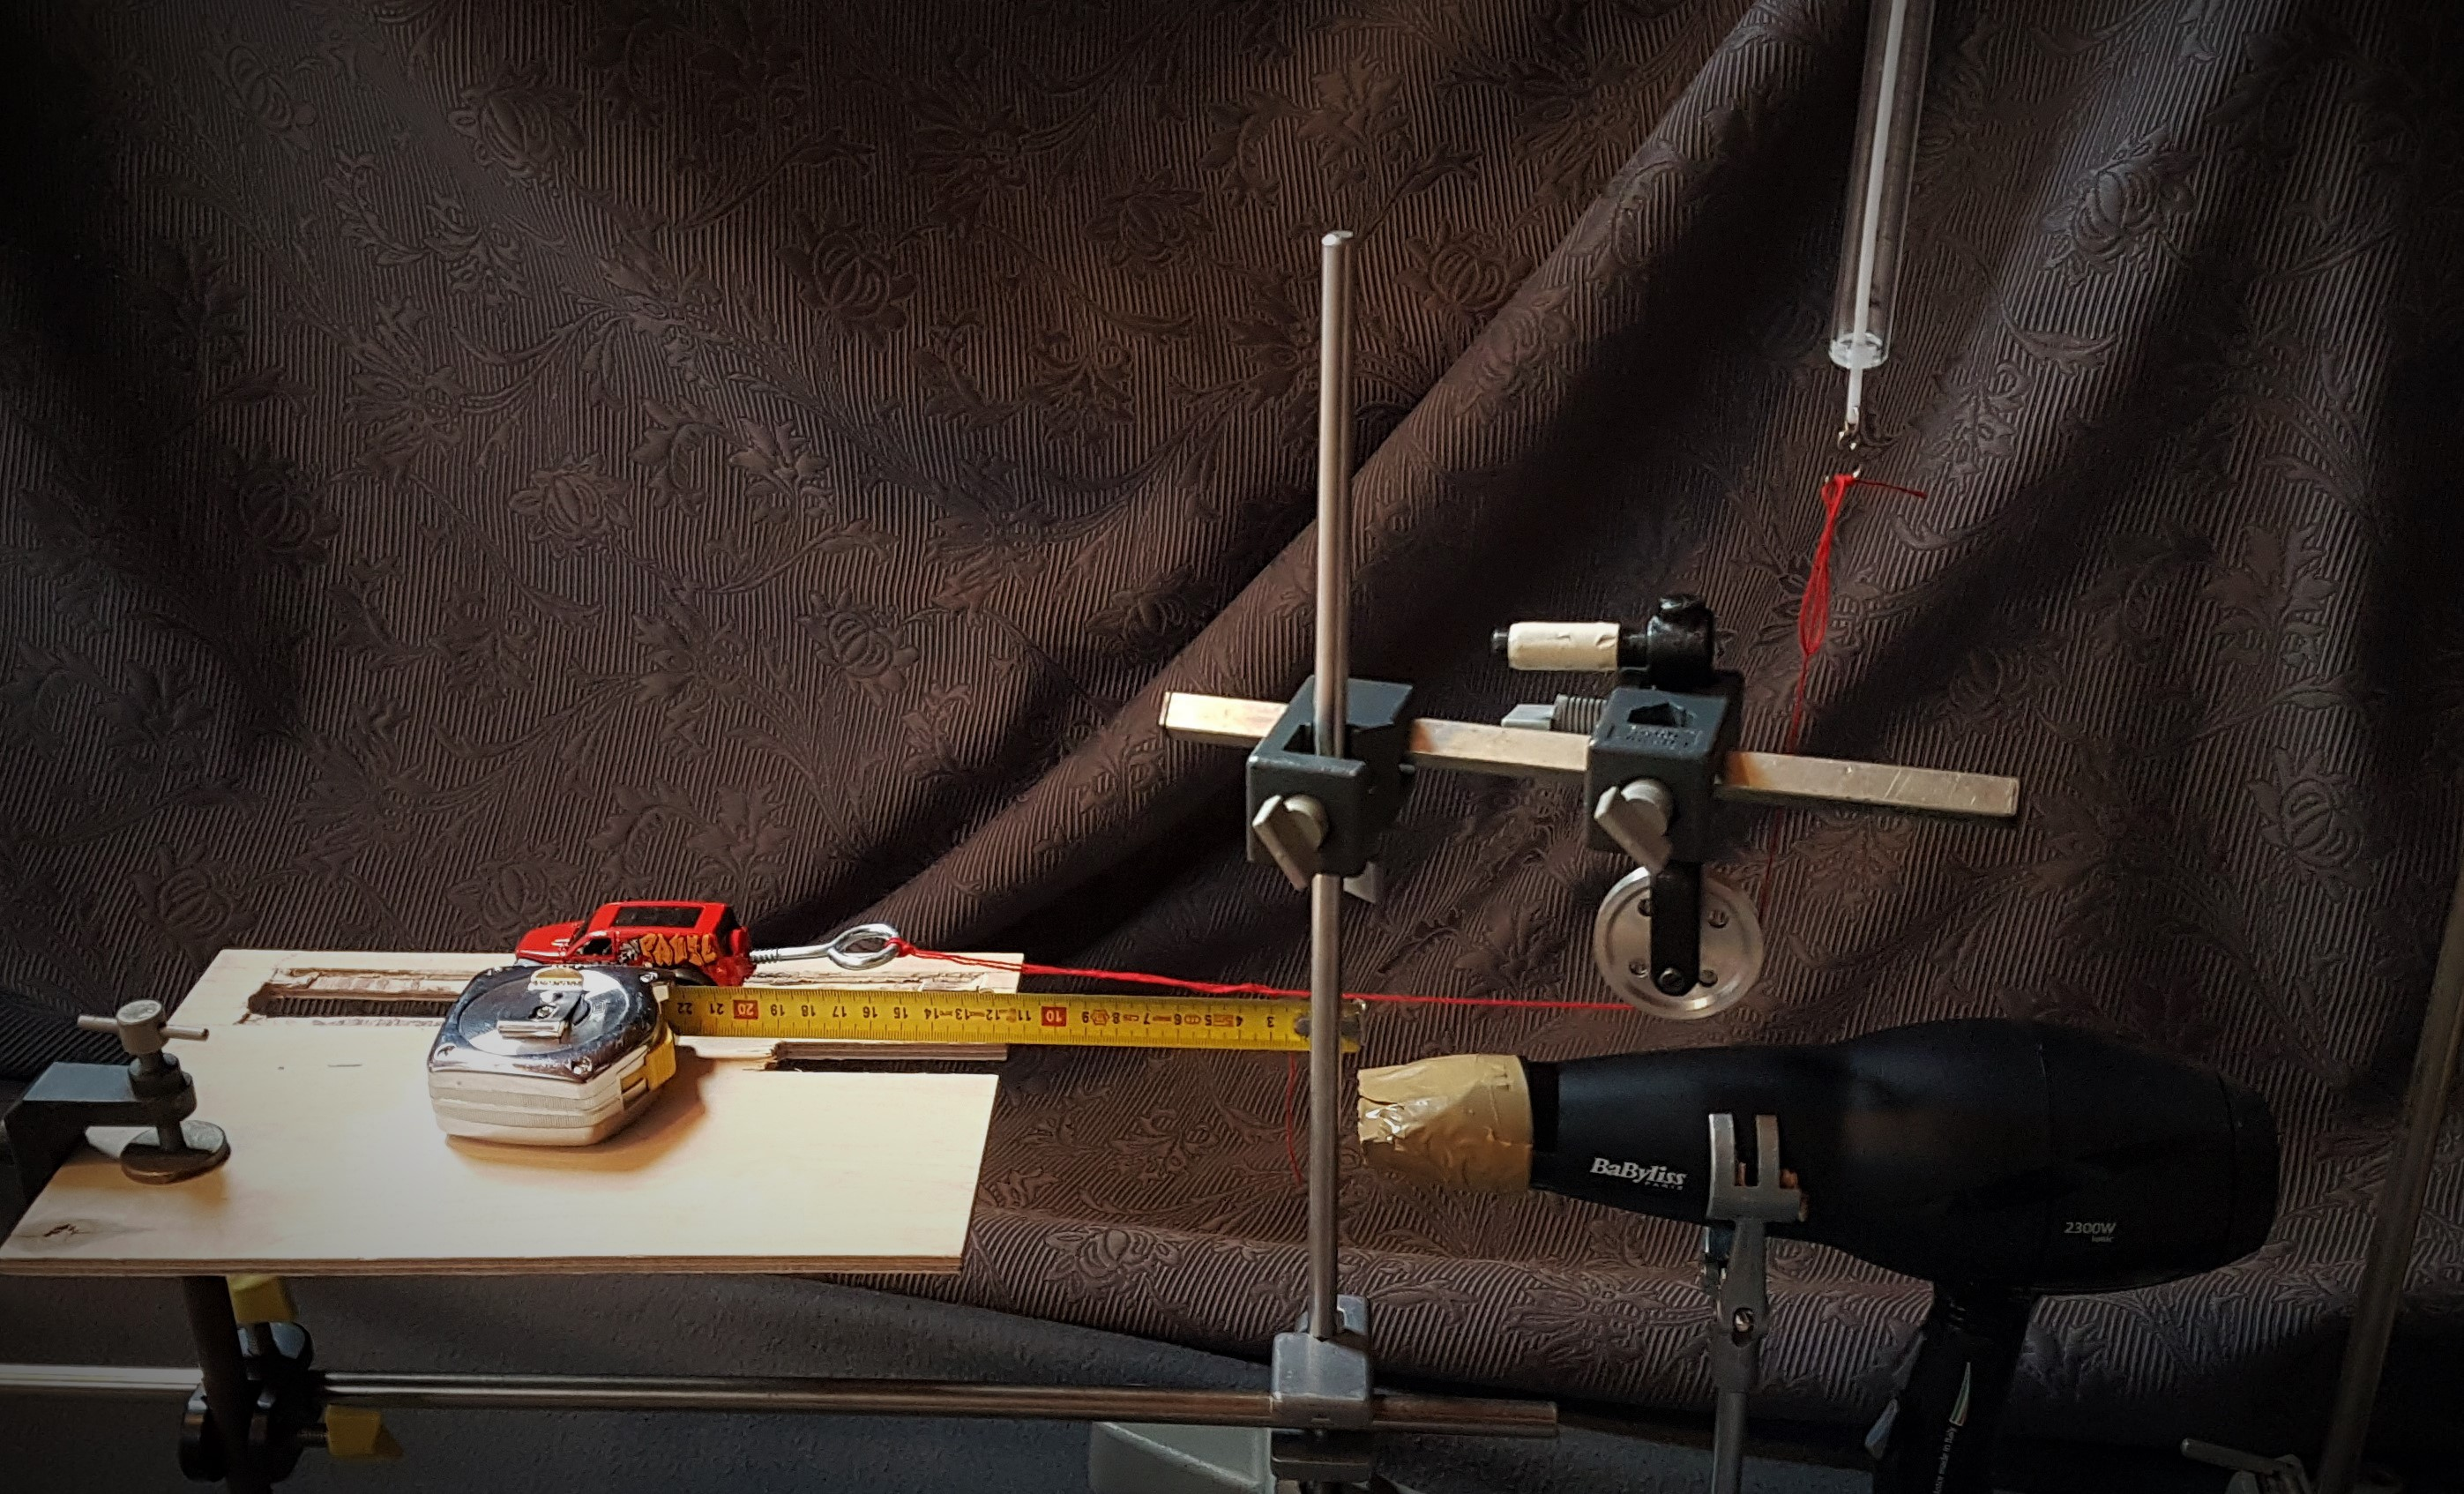
\includegraphics[scale=0.108]{images/stroemungskraftmessung1.jpg}};
     \node (fig2) at (3,40)
       {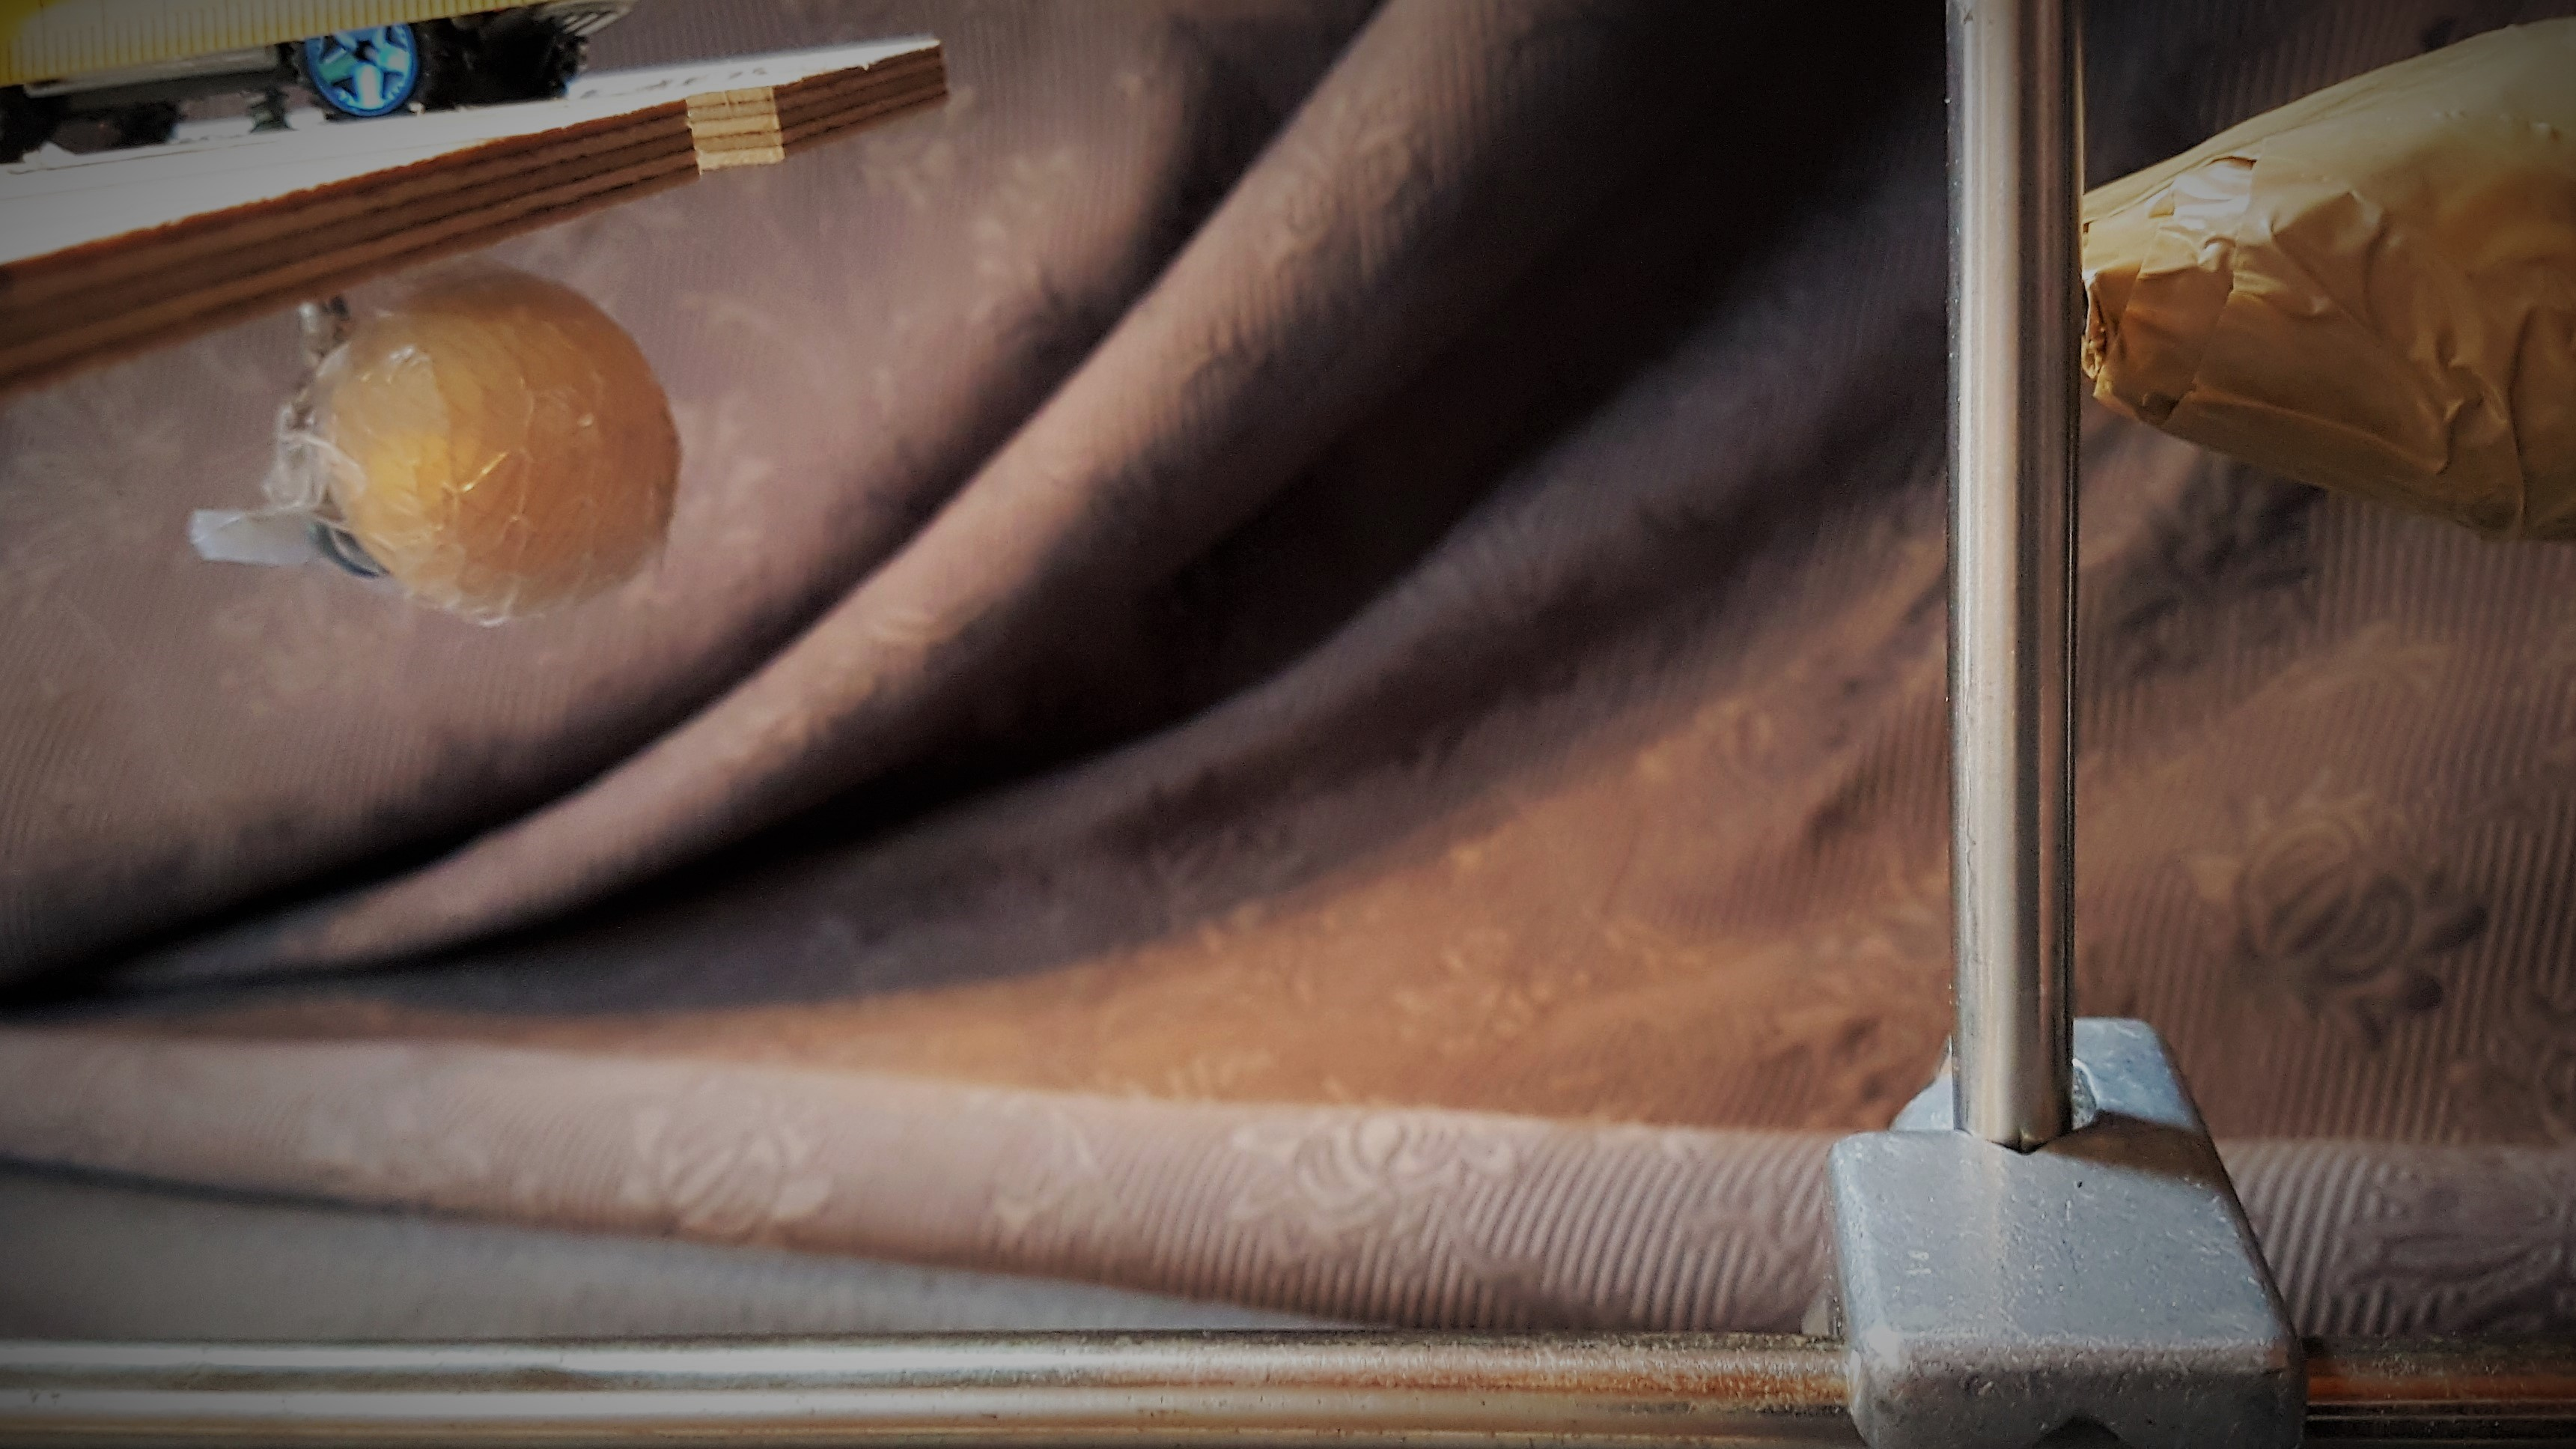
\includegraphics[scale=0.027]{images/stroemungskraftmessung2.jpg}};  
\end{tikzpicture}
  \caption[Erster Versuchsaufbau zur Strömungskraftmessung]{Erster Versuchsaufbau zur Strömungskraftmessung: Ein Messwagen, an dem eine Kugel aufgehängt wird, ist mit einem Federkraftmesser über eine Umlenkrolle verbunden. Die Unterseite der Messplatte ist als Auszug links oben im Foto abgebildet.}
  \label{fig:stroemungskraftmessung1}
  \vspace{-0pt}
\end{figure}

\noindent Hierzu erhält ein Spielzeugauto eine Bohrung durch die Bodenplatte, um mit einem Haken den zu vermessenden Gegenstand anzubringen, und --- für die Verbindung mit dem Kraftmesser --- eine Bohrung am Heck. Als Messfläche wird eine dünne Sperrholzplatte genutzt, in welche eine schmale Aussparung für den unteren Haken gesägt wird. Um die Kraftmessung nur in eine Raumrichtung zuzulassen, werden mit einem Stechbeitel Schienen für den Messwagen in die Platte gehauen. Ein Foto des Versuchsaufbaus ist in Darstellung \ref{fig:stroemungskraftmessung1} abgebildet.

Bereits nach den ersten Messungen stellt sich allerdings heraus, dass der Versuchsaufbau aus mehreren Gründen ungeeignet ist
\begin{items}
\item Federkraftmesser haben einen relativ langen \textit{Hubweg}. Dadurch wird nur für einen Sekundenbruchteil der wahre Abstand des Föhns zu der Kugel vermessen, da der Messwagen einige Zentimeter vorwärts rollt, was in einem Ausschlag des Federkraftmessers auf eine Kraft $N_\mathrm{max}$ gesehen werden kann, deren Anzeigedauer jedoch nicht lang genug für eine Aufzeichnung ist.
\item Bei der Versuchsanordnung befindet sich der Ball nicht unmittelbar unterhalb der Platte, sondern in einem Abstand von ca. $\SI{1}{\centi\metre}$, was für eine Modellierung des Strömungsverhaltens im zu erstellenden Versuchsaufbau nicht hinnehmbar ist. Zudem ist das Sperrholzstück zu kurz, als dass das Gebläse direkt an ihm montiert werden könnte. Für verschiedene Messabstände ist jeweils eine zeitaufwendige Neukalibrierung erforderlich. 
\item Eine Messreihe von ausreichender Größe für eine mathematische Beschreibung benötigt sehr viele Messwerte, die nach \textcite{Schilling1987} im Bereich um $\SI{100}{\milli\newton}$ zu erwarten sind. Ein Federkraftmesser dieser Genauigkeit kann zwar beschafft werden, jedoch erfordern die näheren Föhnabstände $s$ bei größerem Kugelradius $r$ einen weiteren Kraftmesser für einen höheren Messbereich, was eine Vergleichbarkeit der Messungen wiederum unmöglich macht.
\end{items}

%% Autor: Björn Ritterbecks 
%% Letzte Aenderung: 15.06.2016 
\thisfloatsetup{%
  capbesidewidth=\marginparwidth}
\begin{figure}[htbp]
\centering
%\sansmath
 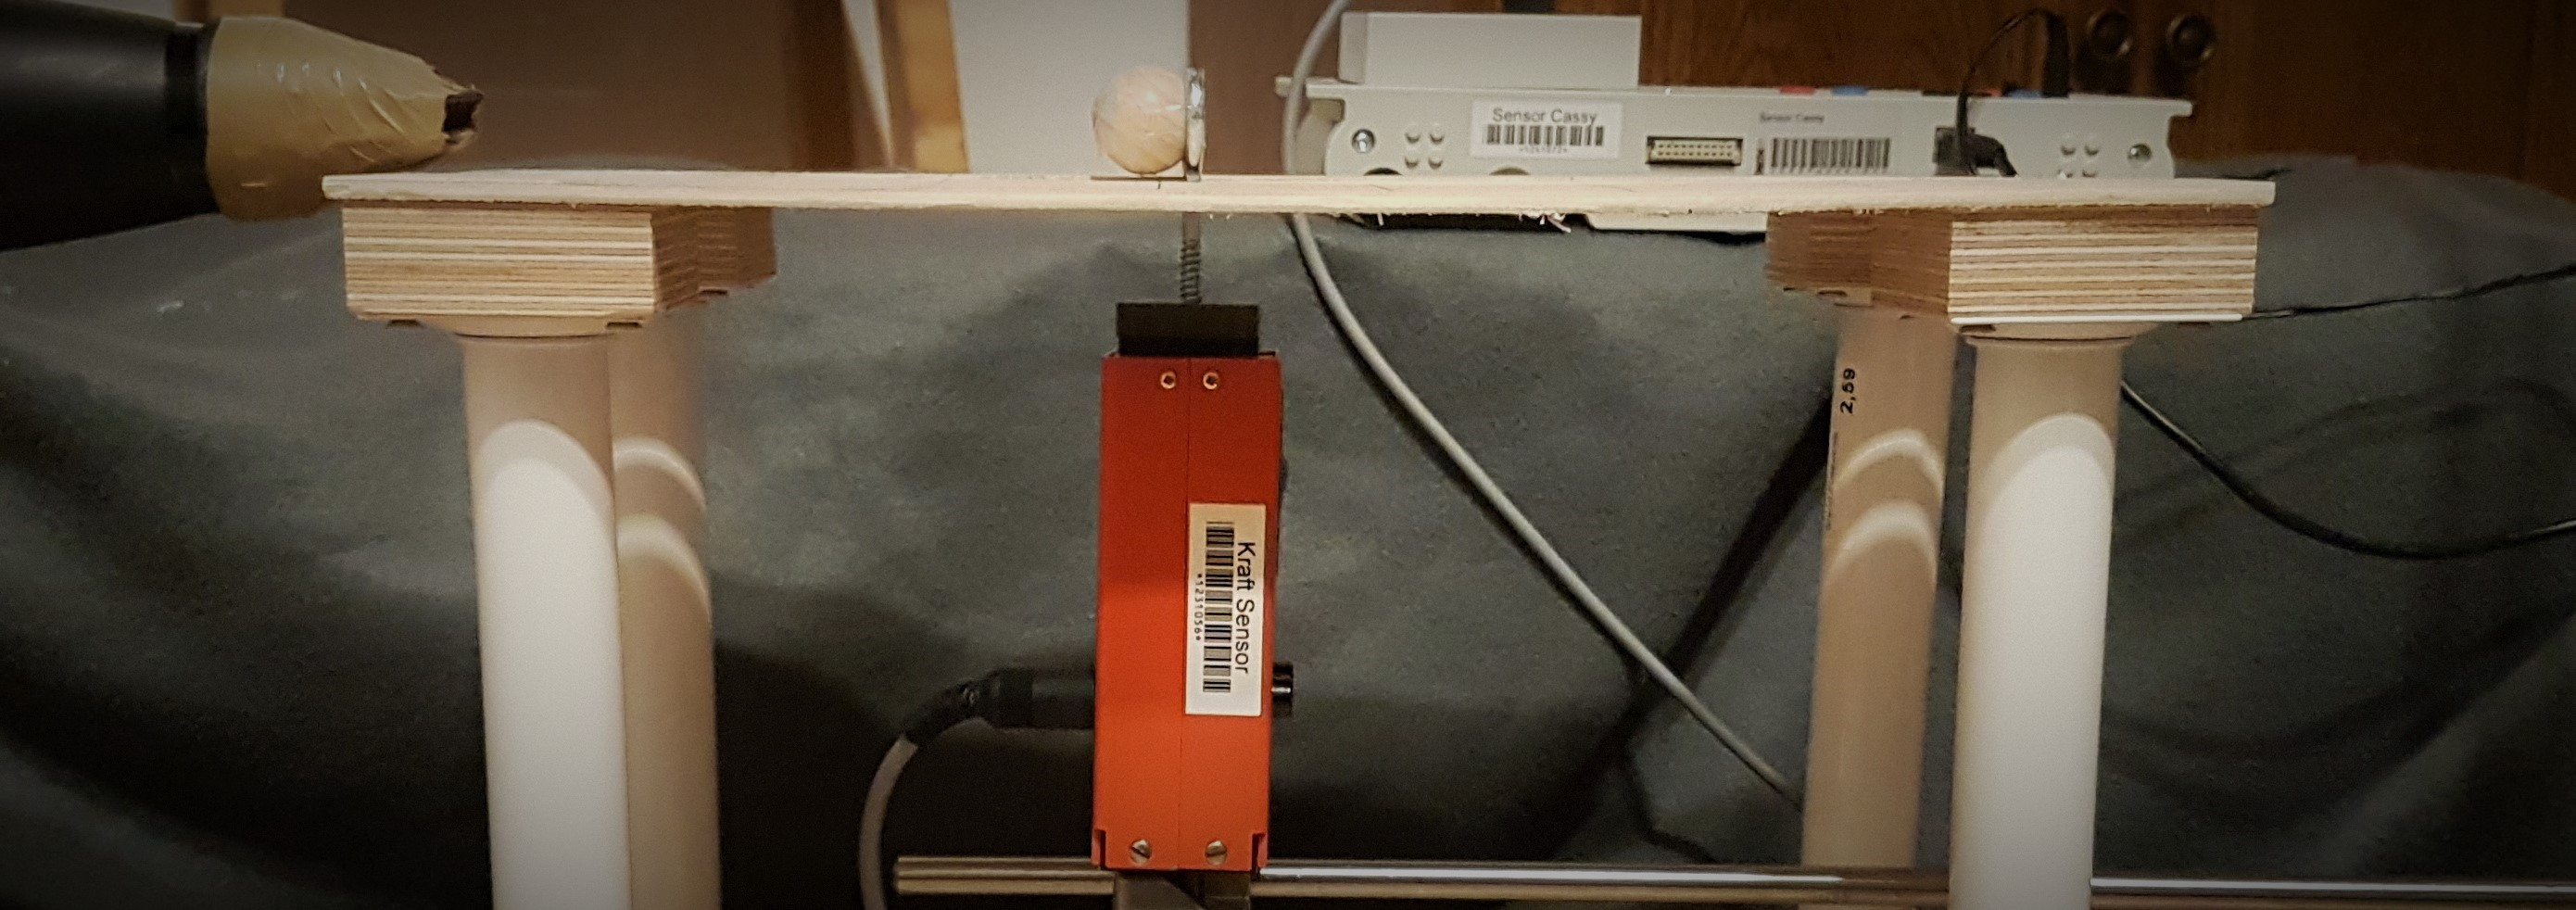
\includegraphics[width=0.99\textwidth]{images/stroemungskraftmessung3.jpg}
  \caption[Coulomb-Kraftmesser der Firma LD Didactic]{Die orange-farbige Box in der Mitte des Fotos vom Messaufbau ist ein Coulomb-Kraftmesser. Dieser ist in $x$-Richtung beweglich an eine Stativstange montiert. Ein eingeschraubter Haken ermöglicht die Befestigung von zu vermessenden Luftwiderständen.}
    \label{fig:stroemungskraftmessung3}
  \vspace{-0pt}
\end{figure}

\noindent Aus einem Schülerversuch sind \textit{Coulomb-Kraftmesser} bekannt (siehe Abbildung \ref{fig:stroemungskraftmessung3}), die auf ein hundertstel $\si{\milli\newton}$ genau messen können und zudem --- laut Herstellerangaben von \textsc{Leybold Didactic}\footnote{vgl. \url{http://www.ld-didactic.de/documents/de-DE/GA/GA/5/524/524060d.pdf}, abgerufen am 29.06.2016} --- einen Hub von lediglich $\pm \SI{0.5}{\milli\metre}$ haben, womit diese Kraftmesser alle zuvor genannten Bedingungen erfüllt. Von Vorteil ist auch, dass durch die Messwerterfassung mit \textsc{Cassy} über ein Zeitintervall gemittelte Werte und damit genauere Ergebnisse möglich sind.

%% Autor: Björn Ritterbecks 
%% Letzte Aenderung: 15.06.2016 
\thisfloatsetup{%
  capbesidewidth=\marginparwidth}
\begin{figure}[htbp]
\centering
%\sansmath
 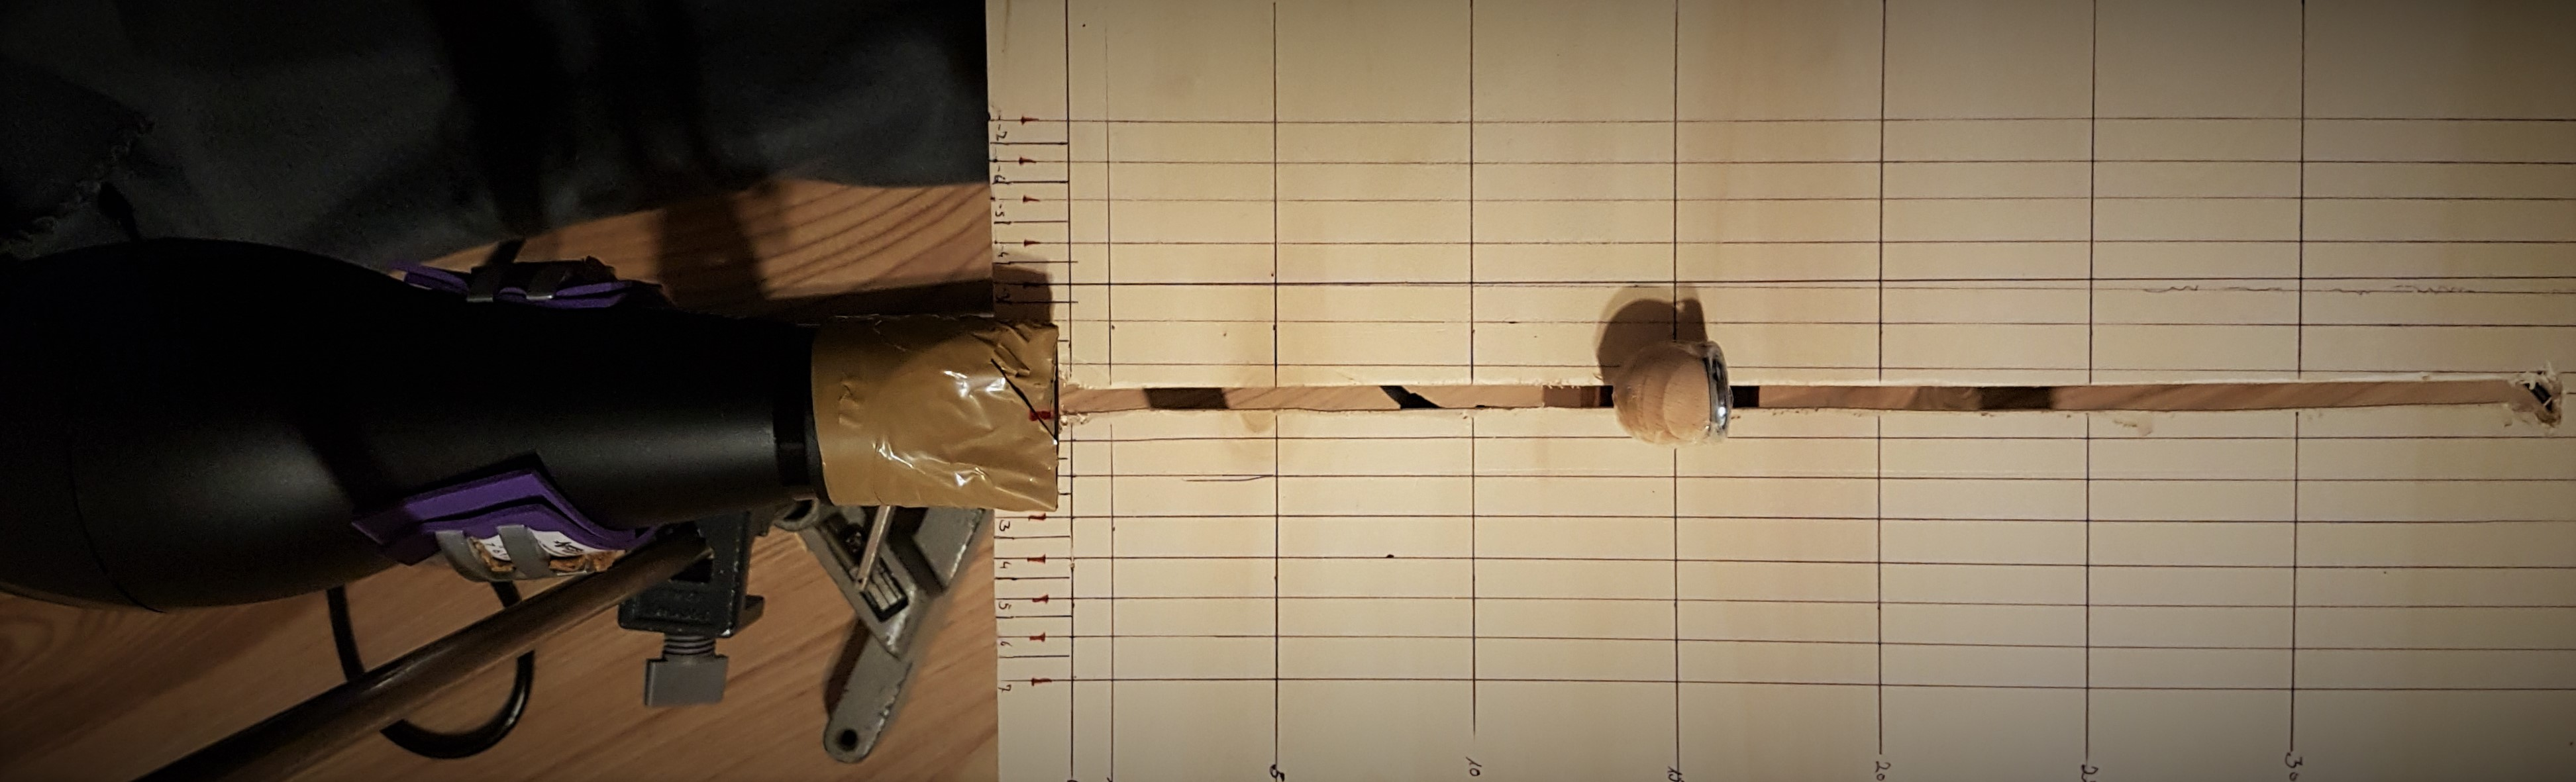
\includegraphics[width=0.99\textwidth]{images/stroemungskraftmessung4.jpg}
  \caption[Zweiter Versuchsaufbau zur Srömungskraftmessung]{Draufsicht des zweiten Versuchsaufbaus für die Messungen zur Strömungswiderstandskraft von Kugeln unterschiedlicher Radien. Ein Föhn ist beweglich auf einem Stativfuß an dem Messtisch angebracht, der mit einem Koordinatensystem für die Messreihen präpariert ist.}
  \label{fig:stroemungskraftmessung4}
  \vspace{-0pt}
\end{figure}

\noindent Ein Messtisch der Länge $l=\SI{35}{\centi\metre}$, der aus Sperrholz und Möbelfüßen schnell hergestellt ist, erhält ein Koordinatensystem, um die Datenerfassung zuverlässig und zügig vornehmen zu können. In die Bohrung des Coulomb-Kraftmessers wird von oben durch eine Ausfräsung des Messtisches ein mit einer Kugel beklebter Haken geschraubt. Durch diesen Aufbau ist es möglich, die Bälle direkt oberhalb der Platte, jedoch reibungsfrei zu lagern. Das Gebläse, wird auf einem schweren Stativ so angebracht, dass die Düsenöffnung $\SI{2}{\centi\metre}$ in die Platte hineinragt.

Die 56 Messreihen (4 Kugelradien á 7 Abstände á 2 Gebläsestufen) werden folgendermaßen aufgezeichnet: Der Kraftmesser wird in einem festen Abstand $s_i$ zum Föhn fixiert. Dieser wird anschließend möglichst parallel zur $x$-Achse auf die $\SI{5}{\milli\metre}$ auseinanderliegenden Messpunkte geführt, wo nach einer Integrationszeit von $\SI{300}{\milli\second}$ der jeweilige Messwert von der Benutzeroberfläche des \textit{Cassy-Lab 2} abgelesen wird. Die ersten beiden Messungen sind in Tabelle \ref{tab:kraftmessung1} aufgelistet.

  \thisfloatsetup{
  capbesidewidth=\marginparwidth,
}
\begin{table}[htb]
\centering
%\sffamily,
\small
%\sansmath
\arrayrulecolor{white}
%\setlength{\arrayrulewidth}{2pt}
\vspace{0.2cm}
  \rowcolors{2}{halfgray!15}{halfgray!5}
 \setlength{\extrarowheight}{.00em}
 \subfloat[$s=\SI{1}{\centi\metre}$]{
			\begin{tabularx}{0.45\textwidth}{r*{2}{>{\RaggedLeft\arraybackslash}X}}	
\rowcolor{mycolor} & 	\multicolumn{2}{c}{{\color{white}\textbf{Kraft in $\boldsymbol{\si{\milli\newton}}$}}} \\
\rowcolor{mycolor}  \multirow{-2}{*}{{\color{white}\textbf{$\boldsymbol{d}$ in $\boldsymbol{\si{\centi\metre}}$}}} & \multicolumn{1}{c}{{\color{white}\textbf{Stufe 2}}} &\multicolumn{1}{c}{{\color{white}\textbf{Stufe 1}}}\\
-4,0	$\pm$	0,1	&	0	&	0	\\
-3,5	$\pm$	0,1	&	6	&	2	\\
-3,0	$\pm$	0,1	&	60	&	42	\\
-2,5	$\pm$	0,1	&	115	&	70	\\
-2,0	$\pm$	0,1	&	150	&	90	\\
-1,5	$\pm$	0,1	&	210	&	122	\\
-1,0	$\pm$	0,1	&	276	&	177	\\
-0,5	$\pm$	0,1	&	303	&	188	\\
0,0	$\pm$	0,1	&	292	&	183	\\
0,5	$\pm$	0,1	&	263	&	165	\\
1,0	$\pm$	0,1	&	214	&	128	\\
1,5	$\pm$	0,1	&	154	&	97	\\
2,0	$\pm$	0,1	&	114	&	68	\\
2,5	$\pm$	0,1	&	75	&	52	\\
3,0	$\pm$	0,1	&	23	&	14	\\
3,5	$\pm$	0,1	&	0	&	0	\\
		\end{tabularx}}
		\quad
 \subfloat[$s=\SI{5}{\centi\metre}$]{
			\begin{tabularx}{0.45\textwidth}{r*{2}{>{\RaggedLeft\arraybackslash}X}}	
\rowcolor{mycolor} & 	\multicolumn{2}{c}{{\color{white}\textbf{Kraft in $\boldsymbol{\si{\milli\newton}}$}}} \\
\rowcolor{mycolor}  \multirow{-2}{*}{{\color{white}\textbf{$\boldsymbol{d}$ in $\boldsymbol{\si{\centi\metre}}$}}} & \multicolumn{1}{c}{{\color{white}\textbf{Stufe 2}}} &\multicolumn{1}{c}{{\color{white}\textbf{Stufe 1}}}\\
-4,0	$\pm$	0,2	&	0	&	0	\\
-3,5	$\pm$	0,2	&	3	&	0	\\
-3,0	$\pm$	0,2	&	32	&	5	\\
-2,5	$\pm$	0,2	&	67	&	35	\\
-2,0	$\pm$	0,2	&	111	&	71	\\
-1,5	$\pm$	0,2	&	170	&	104	\\
-1,0	$\pm$	0,2	&	217	&	145	\\
-0,5	$\pm$	0,2	&	249	&	156	\\
0,0	$\pm$	0,2	&	250	&	157	\\
0,5	$\pm$	0,2	&	235	&	146	\\
1,0	$\pm$	0,2	&	205	&	121	\\
1,5	$\pm$	0,2	&	159	&	84	\\
2,0	$\pm$	0,2	&	114	&	62	\\
2,5	$\pm$	0,2	&	65	&	30	\\
3,0	$\pm$	0,2	&	10	&	2	\\
3,5	$\pm$	0,2	&	0	&	0	\\
		\end{tabularx}}		
		\caption[Exemplarische Kraftmessung des Gebläses]{Exemplarische Kraftmessung des Gebläses für eine Kugel mit $r=\SI{17.5}{\milli\metre}$ bei einem Abstand von \textbf{\color{mycolor}(a)}, $s=\SI{1}{\centi\metre}$ und \textbf{\color{mycolor}(b)}, $s=\SI{5}{\centi\metre}$ vom Föhn, der über zwei Gebläsestufen verfügt. Die Aufnahme der Messdaten erfolgt mit einem \textsw{Coulomb-Kraftmesser}.} 
		\label{tab:kraftmessung1}	
		\end{table} %\vspace*{-5cm}\newpage

\noindent Die Messungenauigkeit auf die Kraft $F_\mathrm{LW}$ beträgt nach den Herstellerangaben des verwendeten Gerätes $\SI{1}{\percent}$, womit sie gegenüber der Justage des Gebläses vernachlässigbar ist. Wird der Haartrockner nicht genau parallel zur $x$-Achse ausgerichtet, so ergibt sich über den Tangens bei zunehmendem Abstand $s$ eine Entfernungsdifferenz $\Delta s$ von bis zu $\SI{1.1}{\centi\metre}$, wenn davon ausgegangen wird, dass die Ausrichtung nur auf $\SI{2}{\degree}$ genau erfolgt (hierzu sei auf grafische Auftragungen wie \ref{fig:kraftmessung9} im Anhang verwiesen, bei denen eine \textit{Schiefe} erkannt werden kann). Selbst bei der als gering angenommenen Abweichung übertrifft diese Unsicherheit diejenige des Messgerätes um den Faktor fünf.

  \thisfloatsetup{%
  capbesidewidth=\marginparwidth}

\begin{figure}[htbp]
\centering
%\sansmath
\subfloat[Stufe 2]{
\begin{tikzpicture}
\begin{axis}[	
	clip=false, % Verhindet weiße Punkte bei vielfach geplotteten x-Werten
	ymajorgrids,
    xmajorgrids,
          axis x line*=middle,
          axis y line*=center,
    grid style={white},
	axis on top,
    width=12cm,
    height=4.797cm,
    xmin=-7,
    xmax=7,
    ymin=0,
    ymax=350,
    %/tikz/ybar interval,
    tick align=center,
    xtick align=outside,
    xlabel={Abstand $d$},
    ylabel={\rotatebox[origin=b]{270}{Windlast $F_\mathrm{LW}$}},   
   x label style={at={(axis cs:5,-65)}},
    y label style={at={(axis cs:-3.5,300)}},
    axis line style={Honeydew4!70!black},
    ticklabel style={Honeydew4!70!black, inner sep=1pt,
                font=\footnotesize},
    yticklabels={${50}$, ${100}$, ${150}$,  ${200}$,   ${250}$ , ${\si{\milli\newton}}$, ${350}$ },            
    ytick={50,100,150,200, 250, 300, 350},
    xticklabels={-7,-5,-3,-1,1,3, $\si{\centi\metre}$, 7},
     xtick={-7,-5,-3,-1,1,3,5, 7}, 
    scaled ticks=false,
    width=\textwidth,                                   
    label style={font=\small,Honeydew4!70!black,},
    enlarge x limits=true,
    %tick style={draw=none},
    x tick label as interval=false,
]
\draw[thick, Honeydew4!70!black, ->,>={latex[Honeydew4!70!black, round, length=0.4cm, width=4pt]}] (axis cs:-3.50, 260) -- (axis cs:-3.50, 340);
\draw[thick,Honeydew4!70!black, ->,>={latex[Honeydew4!70!black,round, length=0.4cm, width=4pt]}] (axis cs:3.00, -65) -- (axis cs:7.00, -65);
\addplot[fill=mycolor4, draw=mycolor4, only marks, mark=*, error bars/.cd,
   x dir=both,
   x explicit, error bar style={mycolor4}]
table[x = x, y =y, x error=dx]{images/data/kraftmessung1S2.dat};
\addplot[mycolor, fill=mycolor!25, smooth, domain=-8:8,thick, opacity=0.4] {302.8*exp(-((x)/2.143)^2)};
\end{axis}
\clipright
\end{tikzpicture}}
\\
\subfloat[Stufe 1]{
\begin{tikzpicture}
\begin{axis}[	
	clip=false, % Verhindet weiße Punkte bei vielfach geplotteten x-Werten
	ymajorgrids,
    xmajorgrids,
          axis x line*=middle,
          axis y line*=center,
    grid style={white},
	axis on top,
    width=12cm,
    height=4.797cm,
    xmin=-7,
    xmax=7,
    ymin=0,
    ymax=350,
    %/tikz/ybar interval,
    tick align=center,
    xtick align=outside,
    xlabel={Abstand $d$},
    ylabel={\rotatebox[origin=b]{270}{Windlast $F_\mathrm{LW}$}},   
   x label style={at={(axis cs:5,-65)}},
    y label style={at={(axis cs:-3.5,300)}},
    axis line style={Honeydew4!70!black},
    ticklabel style={Honeydew4!70!black, inner sep=1pt,
                font=\footnotesize},
    yticklabels={${50}$, ${100}$, ${150}$,  ${200}$,   ${250}$ , ${\si{\milli\newton}}$, ${350}$ },            
    ytick={50,100,150,200, 250, 300, 350},
    xticklabels={-7,-5,-3,-1,1,3, $\si{\centi\metre}$, 7},
     xtick={-7,-5,-3,-1,1,3,5, 7}, 
    scaled ticks=false,
    width=\textwidth,                                   
    label style={font=\small,Honeydew4!70!black,},
    enlarge x limits=true,
    %tick style={draw=none},
    x tick label as interval=false,
]
\draw[thick, Honeydew4!70!black, ->,>={latex[Honeydew4!70!black, round, length=0.4cm, width=4pt]}] (axis cs:-3.50, 260) -- (axis cs:-3.50, 340);
\draw[thick,Honeydew4!70!black, ->,>={latex[Honeydew4!70!black,round, length=0.4cm, width=4pt]}] (axis cs:3.00, -65) -- (axis cs:7.00, -65);
\addplot[fill=mycolor, draw=mycolor, only marks, mark=*, error bars/.cd,
   x dir=both,
   x explicit, error bar style={mycolor}]
table[x = x, y =y, x error=dx]{images/data/kraftmessung1S1.dat};
\addplot[mycolor4, fill=mycolor4!25, smooth, domain=-8:8,thick, opacity=0.4] {188.1*exp(-((x)/2.133)^2)};
\end{axis}
\clipright
\end{tikzpicture}}
  \caption[Beispielhafter Gaußglocken-Fit]{Beispiel eines in \textit{Matlab} erzeugten Gaußglocken-Fits für die Messung der Kugel mit $r=\SI{17.5}{\milli\metre}$ bei einem Abstand von $s=(1.0\pm 0.1)\,\si{\centi\metre}$. Als Anpassungsfunktion wird für alle Messreihen $f(d)=A\cdot \exp(-\left(\sfrac{d-\mu}{2\sigma^2}\right)^2)$ verwendet, da sie im Mittel die geringsten quadratischen Abweichungen bei den vorhandenen Daten liefert. Alle graphischen Auftragungen der Messwerte wurden um das jeweilige $\mu$ verschoben. Die Fehlerbalken sind kaum zu erkennen, da als Unsicherheit auf den Abstand des Gebläses von der Mittelachse ein Winkel von $\varphi=\SI{2}{\degree}$ angenommen wird und damit die Messungenauigkeit linear mit dem Abstand des Föhns skaliert. }
  \label{fig:kraftmessung1}
  \vspace{-0pt}
\end{figure}

\noindent Abbildung \ref{fig:kraftmessung1} zeigt die Diagramme zu den Messwerten aus Tabelle \ref{tab:kraftmessung1}. Die Kurvenanpassung in Form einer Gaussglocke, die mit der Software \textit{Matlab} berechnet wird, folgt dem Modell
\begin{equation}
\label{eq:gebl1}
f(d)=A\cdot \e^{-\left(\frac{d-\mu}{2\sigma^2}\right)^2},
\end{equation}
welches eine klassische \textit{Gaußverteilung} darstellt (siehe Tab. \ref{tab:gaaussfit1}). Werden nun die Integrale unterhalb der Kurven berechnet, so können diese als \textit{an den Kugeln verrichtete Arbeit} $W$ gesehen werden, wobei die Lösung durch die Verschiebung der Messpunkte um $\mu$ das Integral vereinfacht:
\begin{equation}
\label{eq:gebl2}
\begin{alignedat}{2}
 W & = \int_{d_\mathrm{min}}^{d_\mathrm{max}}A\cdot \e^{-\frac{d}{2\sigma^2}^2}\mathrm{d}d\\
 & = \frac{1}{2}\sqrt{\uppi}\cdot A\cdot 2\sigma^2 \cdot \mathrm{erf}(\frac{d}{2\sigma^2}),
\end{alignedat}
\end{equation}
wobei $\mathrm{erf}(\sfrac{d}{2\sigma^2})$ die \textit{gauß'sche Fehlerfunktion}
\begin{equation}
\mathrm{erf}(\frac{d}{2\sigma^2})=\frac{2}{\sqrt{\uppi}}\int_{0}^{\sfrac{d}{2\sigma^2}}\e^{-\tau^2}\mathrm{d}\tau
\end{equation}
bezeichnet. Die Funktion ist punktsymmetrisch zum Koordinatenursprung und konvergiert bereits ab $x=\pm 1$ schnell gegen $\pm 1$. Wie \textsc{Bronstein} aufführt, gilt zudem 
\begin{equation}
2\Phi (x)-1=\mathrm{erf}(\frac{x}{\sqrt{\uppi}}),
\end{equation} 
die Fehlerfunktion kann demnach mit der \textit{Standardnormalverteilung} $\Phi(x)$ berechnet werden.\footfullcite[vgl.][S.\,517]{Bronstein2008}

  \thisfloatsetup{
  capbesidewidth=\marginparwidth,
}
\begin{table}[htb]
\centering
%\sffamily,
\small
%\sansmath
\arrayrulecolor{white}
%\setlength{\arrayrulewidth}{2pt}
\vspace{0.2cm}
  \rowcolors{2}{halfgray!15}{halfgray!5}
 \setlength{\extrarowheight}{.00em}
			\begin{tabularx}{0.99\textwidth}{*{2}{>{\RaggedLeft\arraybackslash}X}X*{3}{>{\RaggedLeft\arraybackslash}X}}	
\rowcolor{mycolor}  {\color{white}\textbf{ Radius $\boldsymbol{r}$ in $\boldsymbol{\si{\milli\metre}}$}} & {\color{white}\textbf{Abstand $\boldsymbol{s}$ in $\boldsymbol{\si{\centi\metre}}$}} & {\color{white}\textbf{Amplitude $\boldsymbol{A}$ in $\boldsymbol{\si{\milli\newton}}$}} & {\color{white}\textbf{$\boldsymbol{\mu}$}} & {\color{white}\textbf{$\boldsymbol{2\sigma^2}$}}& {\color{white}\textbf{$\boldsymbol{R^2}$}}\\
	&	1	&	302,8	&	2,143	&	-0,240	&	0,994	\\
	&	5	&	260,4	&	2,099	&	-0,050	&	0,993	\\
	&	10	&	183,9	&	2,378	&	-0,378	&	0,993	\\
	&	15	&	152,8	&	2,349	&	-0,201	&	0,995	\\
	&	20	&	121,4	&	2,604	&	-0,404	&	0,997	\\
	&	25	&	95,2	&	3,650	&	-0,444	&	0,986	\\
\multirow{-7}{*}{17,5}	&	30	&	73,2	&	3,518	&	-0,626	&	0,992	\\\midrule
	&	1	&	230,9	&	1,903	&	-0,268	&	0,997	\\
	&	5	&	199,2	&	1,912	&	-0,489	&	0,988	\\
	&	10	&	140,9	&	2,201	&	-0,564	&	0,988	\\
	&	15	&	106,5	&	2,381	&	-0,452	&	0,997	\\
	&	20	&	85,2	&	2,609	&	-0,374	&	0,997	\\
	&	25	&	65,7	&	3,237	&	-0,746	&	0,996	\\
\multirow{-7}{*}{15,0}	&	30	&	55,9	&	3,755	&	-0,526	&	0,978	\\\midrule
	&	1	&	157,9	&	1,870	&	-0,484	&	0,994	\\
	&	5	&	139,7	&	1,923	&	-0,660	&	0,988	\\
	&	10	&	100,9	&	1,873	&	-0,596	&	0,994	\\
	&	15	&	73,3	&	2,219	&	-0,855	&	0,995	\\
	&	20	&	60,1	&	2,665	&	-0,345	&	0,994	\\
	&	25	&	44,9	&	2,868	&	-1,262	&	0,996	\\
\multirow{-7}{*}{12,5}	&	30	&	39,9	&	3,689	&	-1,572	&	0,992	\\\midrule
	&	1	&	104,1	&	1,733	&	-0,631	&	0,996	\\
	&	5	&	83,6	&	1,693	&	-0,501	&	0,988	\\
	&	10	&	66,7	&	1,799	&	-0,496	&	0,993	\\
	&	15	&	49,9	&	1,735	&	-0,492	&	0,990	\\
	&	20	&	38,9	&	2,302	&	-0,594	&	0,991	\\
	&	25	&	29,3	&	2,512	&	-0,780	&	0,976	\\
\multirow{-7}{*}{10,0}	&	30	&	25,2	&	2,768	&	-1,538	&	0,987	\\
		\end{tabularx}
		\caption[Ergebnisse der Gaußanpassungen für die höhere Gebläsestufe]{Ergebnisse der Gauß-Anpassungen für die Messreihen auf der höheren Gebläsestufe. $\mu$ und $\sigma$ sind ohne Einheit aufgeführt, da das Argument einer Exponentialfunktion stets dimensionslos ist. Wollte man sie mit aufführen, so wäre $[\mu]=\si{\metre}$ und $[\sigma] = \sqrt{\si{\metre}}$. Als Bestimmtheitsmaß wird $R^2$ gewählt, das für eine Anpassung, die keine \textsw{Residuen} übriglasst, den Wert eins annimmt.}
		\label{tab:gaaussfit1}	
		\end{table} %\vspace*{-5cm}\newpage

\noindent\textcite{Schilling1987} nehmen als verrichtete Arbeit das gesamte Integral unter $F_\mathrm{LW}(d)$ an. Sind die Kugeln jedoch weiter von dem Gebläse entfernt, sind sie aufgrund der Anordnung des Analogieexperiments mit seinen zwei disjunkten Platten diejenigen, welche zu den \textit{schnellen} (nur bis zu $\SI[fraction-function=\sfrac]{1}{\metre\per\second}$, womit das Adjektiv nicht überbewertet werden sollte) Kugeln gezählt werden, kürzer im Zentrum des Strömungsfeldes. 
Als Richtwert wird daher angenommen, dass sich die Kugeln bei einer Fixierung der Gebläse-Position bei $x=\SI{0}{\centi\metre}$ von $x=-\SI{3}{\centi\metre}$ bis $x=\SI{3}{\centi\metre}$ im Strömungsfeld befinden.

  \thisfloatsetup{%
  capbesidewidth=\marginparwidth
  }
\begin{figure}[htbp]
\centering
%\sansmath
\subfloat[]{
\begin{tikzpicture}
\begin{scope}[scale=0.98]
\begin{axis}[	
	clip=false, % Verhindet weiße Punkte bei vielfach geplotteten x-Werten
	ymajorgrids,
    xmajorgrids,
          axis x line*=middle,
          axis y line*=center,
    grid style={white},
	axis on top,
    width=\textwidth,  
    height=6.797cm,
    xmin=0,
    xmax=30,
    ymin=0,
    ymax=1200,
    %/tikz/ybar interval,
    tick align=center,
    xtick align=outside,
    xlabel={Entfernung $s$},
    ylabel={\rotatebox[origin=b]{270}{Arbeit $W$}},   
   x label style={at={(axis cs:25,-150)}},
    y label style={at={(axis cs:-3.0,780)}},
    axis line style={Honeydew4!70!black},
    ticklabel style={Honeydew4!70!black, inner sep=1pt,
                font=\footnotesize},
    yticklabels={${200}$, ${400}$, ${600}$,  ${800}$,  ${\si{\milli\newton\centi\metre}}$, ${1200}$ },            
    ytick={200,400,600, 800, 1000, 1200},
    xticklabels={0, 5, 10, 15, 20, $\si{\centi\metre}$, 30},
     xtick={0,5,10,15,20,25,30}, 
    scaled ticks=false,           
           legend style ={ at={(axis cs:30,1200)}, 
     anchor=north east, draw=none, 
         fill=none,align=left, text=Honeydew4!70!black,
          font=\footnotesize},               
    label style={font=\small,Honeydew4!70!black,},
    cycle list name=mycolor4 white,
    enlarge x limits=true,
    %tick style={draw=none},
    x tick label as interval=false,
]
\draw[thick, Honeydew4!70!black, ->,>={latex[Honeydew4!70!black, round, length=0.4cm, width=4pt]}] (axis cs:-5.50, 850) -- (axis cs:-5.50, 1150);
\draw[thick,Honeydew4!70!black, ->,>={latex[Honeydew4!70!black,round, length=0.4cm, width=4pt]}] (axis cs:21.00, -150) -- (axis cs:29.00, -150);
\addplot
table[x = x, y =y]{images/data/work1.dat};
\addlegendentry{$\SI{17.5}{\milli\metre}$};
\addplot
table[x = x, y =y]{images/data/work2.dat};
\addlegendentry{$\SI{15.0}{\milli\metre}$};
\addplot
table[x = x, y =y]{images/data/work3.dat};
\addlegendentry{$\SI{12.5}{\milli\metre}$};
\addplot
table[x = x, y =y]{images/data/work4.dat};
\addlegendentry{$\SI{10.0}{\milli\metre}$};
\end{axis}
\end{scope}
\clipright
\end{tikzpicture}}
\\
\subfloat[]{
\begin{tikzpicture}
\begin{scope}[scale=0.98]
\begin{axis}[	
	clip=false, % Verhindet weiße Punkte bei vielfach geplotteten x-Werten
	ymajorgrids,
    xmajorgrids,
          axis x line*=middle,
          axis y line*=center,
    grid style={white},
%	axis on top,
    width=\textwidth,  
    height=6.797cm,
    xmin=0,
    xmax=30,
    ymin=0,
    ymax=1200,
    %/tikz/ybar interval,
    tick align=center,
    xtick align=outside,
    xlabel={Entfernung $s$},
    ylabel={\rotatebox[origin=b]{270}{Arbeit $W$}},   
   x label style={at={(axis cs:25,-150)}},
    y label style={at={(axis cs:-3.0,780)}},
    axis line style={Honeydew4!70!black},
    ticklabel style={Honeydew4!70!black, inner sep=1pt,
                font=\footnotesize},
    yticklabels={${200}$, ${400}$, ${600}$,  ${800}$,  ${\si{\milli\newton\centi\metre}}$, ${1200}$ },            
    ytick={200,400,600, 800, 1000, 1200},
    xticklabels={0, 5, 10, 15, 20, $\si{\centi\metre}$, 30},
     xtick={0,5,10,15,20,25,30}, 
    scaled ticks=false,           
           legend style ={ at={(axis cs:30,1200)}, 
     anchor=north east, draw=none, 
         fill=none,align=left, text=Honeydew4!70!black,
          font=\footnotesize},               
    label style={font=\small,Honeydew4!70!black,},
    cycle list name=mycolor white,
    enlarge x limits=true,
    %tick style={draw=none},
    x tick label as interval=false,
]
\draw[thick, Honeydew4!70!black, ->,>={latex[Honeydew4!70!black, round, length=0.4cm, width=4pt]}] (axis cs:-5.50, 850) -- (axis cs:-5.50, 1150);
\draw[thick,Honeydew4!70!black, ->,>={latex[Honeydew4!70!black,round, length=0.4cm, width=4pt]}] (axis cs:21.00, -150) -- (axis cs:29.00, -150);
\addplot
table[x = x, y =y]{images/data/work1.dat};
\addlegendentry{$\SI{17.5}{\milli\metre}$};
\addplot
table[x = x, y =y]{images/data/work5.dat};
\addlegendentry{$\SI{15.0}{\milli\metre}$};
\addplot
table[x = x, y =y]{images/data/work6.dat};
\addlegendentry{$\SI{12.5}{\milli\metre}$};
\addplot
table[x = x, y =y]{images/data/work7.dat};
\addlegendentry{$\SI{10.0}{\milli\metre}$};
\addplot[mycolor, fill=none, smooth, domain=0:31,thick] {0.7145*\x^2-45.18*\x+1093};
\end{axis}
\end{scope}
\clipright
\end{tikzpicture}}
  \caption[An einer vorbeirollenden Kugel verrichtete Arbeit]{Geplottet sind die Arbeitsintegrale nach Gleichung \eqref{eq:gebl2}. {\color{mycolor}\textbf{(a)}:} Je kleiner der Kugelradius $r$, desto geringer ist die Strömungswiderstandskraft und damit auch das Integral über selbige. {\color{mycolor}\textbf{(a)}:} Durch Multiplikation der Arbeitsintegrale mit den Proportionalitätsfaktoren, welche aus den Kugelprojektionsflächen berechnet werden, kann die lineare Skalierung gezeigt werden.}
  \label{fig:workwork}
  \vspace{-0pt}
\end{figure}

\noindent Durch die Gleichung \eqref{eq:gebl2} werden die Arbeitsintegrale für die Sphären mit den Radien $r_1=\SI{10,0}{\milli\metre}$, $r_2=\SI{12,5}{\milli\metre}$, $r_3=\SI{15,0}{\milli\metre}$ und $r_4=\SI{17,5}{\milli\metre}$ berechnet. Mit Erinnerung an Abschnitt \ref{sec:umsetzung} wird von einer Proportionalität der Arbeit und damit auch der Impulsänderung mit der Projektionsfläche der Kugeln ausgegangen. Hierbei gilt $A_\mathrm{proj_1}\cdot 3,06=A_\mathrm{proj_2}\cdot 1,96=A_\mathrm{proj_3}\cdot 1,36=A_\mathrm{proj_4}$. Die Integrale sind in Abbildung \ref{fig:workwork} für die einzelnen Messreihen aufgetragen. Es ist gut zu sehen, dass die Hypothese angenommen werden kann, obwohl zwei Messreihen für die Kugel mit dem Radius $\SI{10}{\milli\metre}$ um bis zu $\SI{20}{\percent}$ unter den erwarteten Werten liegen. Für die eingezeichnete polynomische Anpassung wurde daher die kleinste Kugel nicht berücksichtigt.

\section{Geschwindigkeitsmessung der Anströmung}

Mit der ausgemessenen Kraftwirkung können ebenfalls die Widerstandsbeiwerte $c_\mathrm{W}$ berechnet und mit den Literaturwerten aus \ref{tab:cwwerte} verglichen werden, sofern die Geschwindigkeit der Anströmung bekannt ist.
Zu diesem Zweck wird ein simples \textit{Anemometer} \footnote{Windgeschwindigkeitsmesser} gebaut. Die Konstruktion kann an dem Foto \ref{fig:windgeschw1} erläutert werden:

%% Autor: Björn Ritterbecks 
%% Letzte Aenderung: 15.06.2016 
\thisfloatsetup{%
  capbesidewidth=\marginparwidth}
\begin{figure}[htbp]
\vspace*{0.2cm}
\centering
%\sansmath
 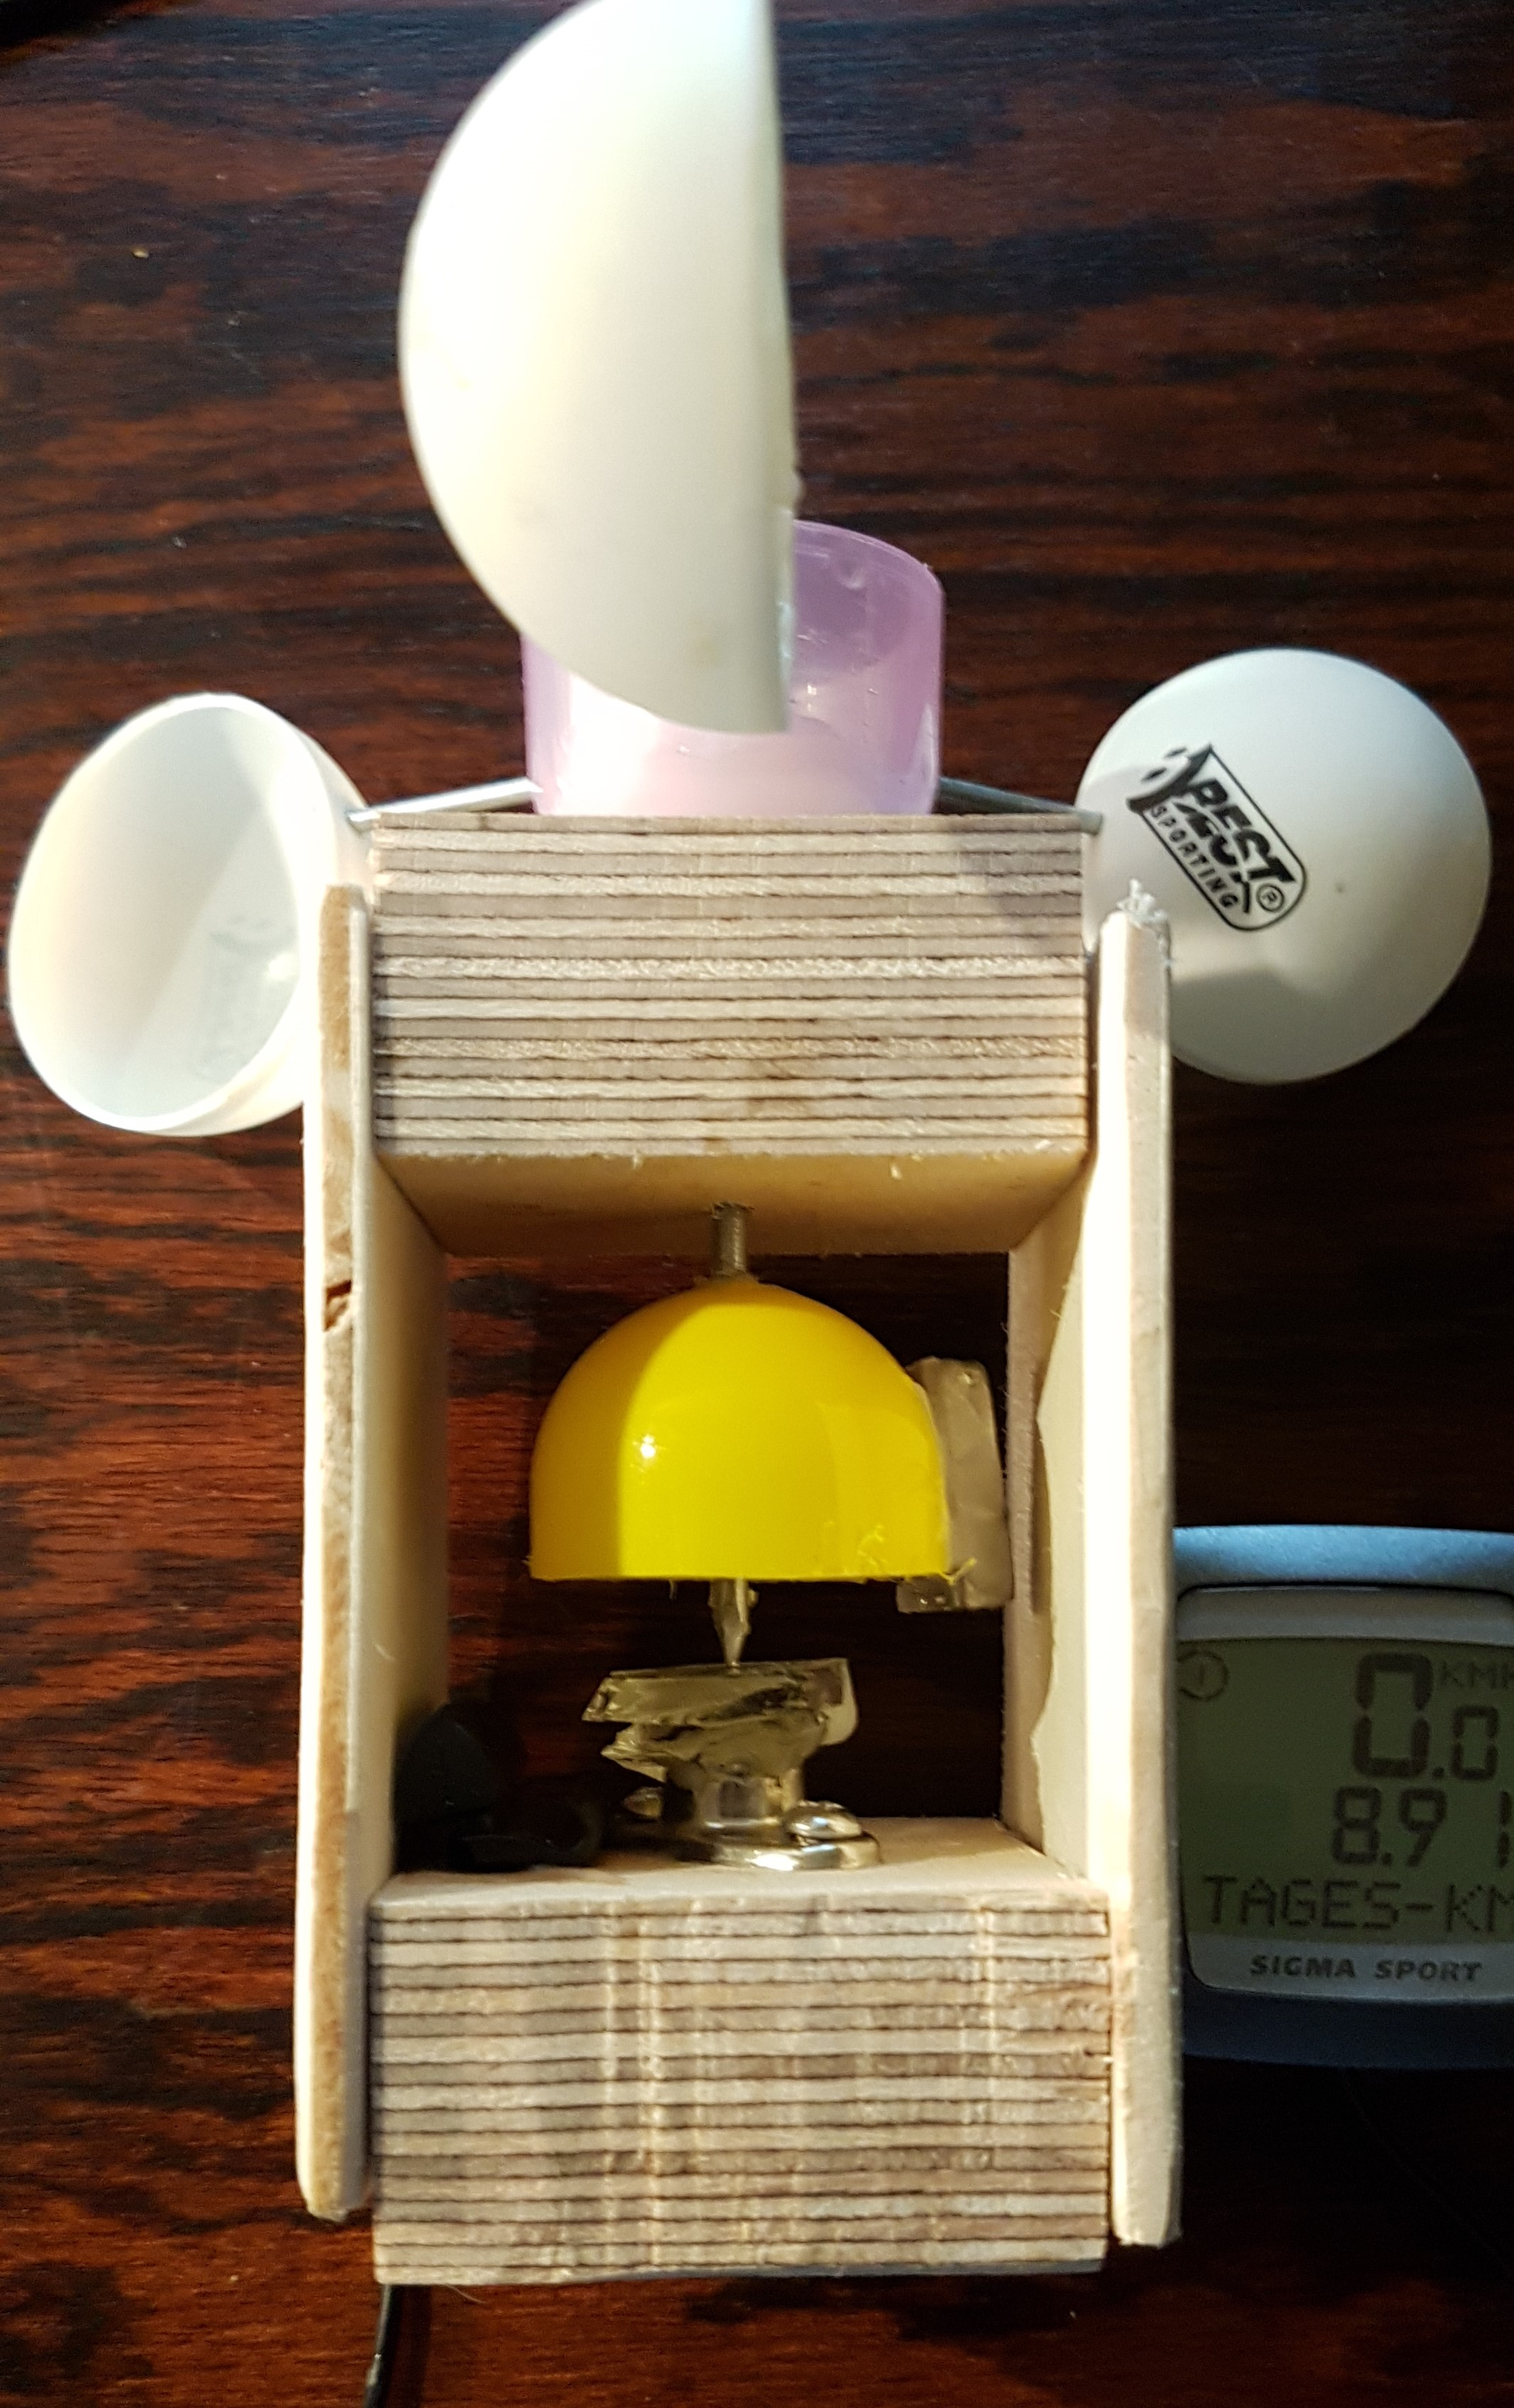
\includegraphics[width=0.75\textwidth]{images/Windkraft.jpg}
  \caption[Selbstbau eines Anemometers]{Aus einfachen Materialien und einem Fahrradcomputer gebautes Anemometer. Die Idee hinter dem Funktionsprinzip kommt von \textsc{Rüdiger Stenzel}: \url{http://www.dc4fs.de/wetter/anemo.htm}. Die Tischtennisballhälften drehen sich bei einem Luftstrom und versetzen damit einen Stahlstift in Rotation, an dem wiederum ein Magnet befestigt ist, der bei jeder Umdrehung durch einen \textsc{Reed-Kontakt} detektiert wird.}
  \label{fig:windgeschw1}
  \vspace{-0pt}
\end{figure}

\noindent Zwei Tischtennisbälle werden halbiert, um möglichst leichte Schalen zu erhalten. Am Rand jeder Hälfte wird ein kleines Loch gebohrt, durch welches ein Stahlnagel von $\SI{30}{\milli\metre}$ Länge gesteckt und anschließend eingeklebt wird. Drei dergestalt präparierte Schalen steckt man nun --- jeweils um $\SI{120}{\degree}$ gegeneinander verschränkt --- durch Bohrungen in der Verschlusskappe eines Kosmetikartikels oder ähnlichem. Hierbei fixieren die drei kurzen Stifte auch einen weiteren Nagel von mindestens $\SI{60}{\milli\metre}$ Länge, der orthogonal und mittig platziert wird, bevor die Kappe mit \textit{Epoxidharz} aufgefüllt wird.

Durch ein Stück dickeren Sperrholzes (in der Abbildung $\SI{30}{\milli\metre}$) wird ein Loch von $\SI{4}{\milli\metre}$ Durchmesser gebohrt, in welches ein passend abgelängter Teil eines Messingrohres mit gleichem Außendurchmesser eingeschlagen wird, um den langen Nagel möglichst \textit{lotrecht} durchzuführen. An dem unteren Ende des Stahlstiftes wird eine weitere Halbschale fixiert, an welcher ein Magnet angeklebt ist (Mitte rechts im Bild). 

Der durch das Rohr geführte Stahlstift dreht sich durch einen Luftstrom bei geringer Reibung auf einer Glasscherbe, die auf die Bodenplatte geklebt ist. Rechts unten in dem Gehäuse befindet sich ein \textit{Reed-Kontakt}, der beim Passieren des Magneten schließt. Durch Vermessen der Distanz von den Schalenmitten zu dem Stahlstift wird der \textit{Radumfang} am Fahrradcomputer eingegeben.

  \thisfloatsetup{
  capbesidewidth=\marginparwidth,
}
\begin{table}[htb]
\centering
%\sffamily,
\small
%\sansmath
\arrayrulecolor{white}
%\setlength{\arrayrulewidth}{2pt}
\vspace{0.2cm}
  \rowcolors{2}{halfgray!15}{halfgray!5}
 \setlength{\extrarowheight}{.00em}
			\begin{tabularx}{0.99\textwidth}{*{3}{>{\RaggedLeft\arraybackslash}X}}	
\rowcolor{mycolor}  \multicolumn{1}{c}{\color{white}\textbf{Entfernung $\boldsymbol{s}$}} & \multicolumn{2}{c}{\color{white}\textbf{Strömungsgeschwindigkeit $\boldsymbol{v}$ in $\boldsymbol{\si{\metre\per\second}}$}}\\ \rowcolor{mycolor} \multicolumn{1}{c}{\color{white}\textbf{in $\boldsymbol{\si{\centi\metre}}$}}& \multicolumn{1}{c}{\color{white}\textbf{Stufe 1}}& \multicolumn{1}{c}{\color{white}\textbf{Stufe 2}}\\
1,0	$\pm$	0,1		&	115	$\pm$	12	&	91	$\pm$	9	\\
5,0	$\pm$	0,2		&	106	$\pm$	11	&	84	$\pm$	8	\\
10,0	$\pm$	0,3		&	93	$\pm$	9	&	73	$\pm$	7	\\
15,0	$\pm$	0,5		&	82	$\pm$	8	&	61	$\pm$	6	\\
20,0	$\pm$	0,7		&	73	$\pm$	7	&	57	$\pm$	6	\\
25,0	$\pm$	0,9		&	65	$\pm$	7	&	51	$\pm$	5	\\
30,0	$\pm$	1,1		&	58	$\pm$	6	&	45	$\pm$	5	\\
		\end{tabularx}
		\caption[Luftgeschwindigkeitsmessung am Gebläse]{Auflistung der Luftgeschwindigkeiten des Gebläses. In dieser Messreihe wird der Haartrockner an der linken Seite des Anemometers, mit der Düse genau mittig vor einer Kugelschale, positioniert.}
		\label{tab:windspeed}	
		\end{table} %\vspace*{-5cm}\newpage

\noindent Die Verifikation der Justierung erfolgt, indem der Anemometer bei eingeschaltetem Tempomat eines Autos möglichst weit aus dem (Beifahrer-) Fenster gehalten wird. 
Mit diesem Messgerät werden die Strömungsgeschwindigkeiten des Föhns für die Entfernungen $s_i$ bestimmt und in Tabelle \ref{tab:windspeed} aufgelistet, wobei eine Messungenauigkeit von $\SI{10}{\percent}$ auf die Geschwindigkeit und die bereits genannten --- über den Tangens berechneten --- Werte für den Gebläseabstand angenommen werden. 

  \thisfloatsetup{
  capbesidewidth=\marginparwidth,
}
\begin{table}[htb]
\centering
%\sffamily,
\small
%\sansmath
\arrayrulecolor{white}
%\setlength{\arrayrulewidth}{2pt}
\vspace{0.2cm}
  \rowcolors{2}{halfgray!15}{halfgray!5}
 \setlength{\extrarowheight}{.00em}
			\begin{tabularx}{0.99\textwidth}{*{2}{>{\RaggedLeft\arraybackslash}X}r*{2}{>{\RaggedLeft\arraybackslash}X}}		
\rowcolor{mycolor}  
%\multicolumn{1}{c}{\color{white}\textbf{Radius $\boldsymbol{r}$}} &
\multicolumn{1}{c}{\color{white}\textbf{Abstand $\boldsymbol{s}$}} &  \multicolumn{1}{c}{\color{white}\textbf{ $\boldsymbol{10^{-3}\cdot R\kern-.04em e}$}} &  \multicolumn{1}{c}{\color{white}\textbf{$\boldsymbol{c_\mathrm{W,\, exp}}$}} &  \multicolumn{1}{c}{\color{white}\textbf{$\boldsymbol{c_\mathrm{W,\, theo}}$}} &  \multicolumn{1}{c}{\color{white}\textbf{Abweichung}}\\ \rowcolor{mycolor}
% \multicolumn{1}{c}{\color{white}\textbf{in $\boldsymbol{\si{\milli\metre}}$}} &
  \multicolumn{1}{c}{\color{white}\textbf{in $\boldsymbol{\si{\centi\metre}}$}} &  \multicolumn{1}{c}{\color{white}\textbf{o.\,E.}} &  \multicolumn{1}{c}{\color{white}\textbf{o.\,E.}} &  \multicolumn{1}{c}{\color{white}\textbf{o.\,E.}} &  \multicolumn{1}{c}{\color{white}\textbf{in $\si{\percent}$}}\\
1,0	$\pm$	0,1	&	78,46	&	0,49	&	0,50	&	-0,4	\\
5,0	$\pm$	0,2	&	72,32	&	0,50	&	0,49	&	1,3	\\
10,0	$\pm$	0,3	&	63,45	&	0,46	&	0,49	&	-5,1	\\
15,0	$\pm$	0,5	&	55,95	&	0,49	&	0,48	&	2,6	\\
20,0	$\pm$	0,7	&	49,81	&	0,50	&	0,47	&	5,3	\\
25,0	$\pm$	0,9	&	44,35	&	0,50	&	0,47	&	7,0	\\
30,0	$\pm$	1,1	&	30,70	&	0,47	&	0,46	&	2,1	\\
		\end{tabularx}
		\caption[Gegenüberstellung experimenteller und theoretischer $c_\mathrm{W}$-Werte]{Gegenüberstellung experimenteller und theoretischer $c_\mathrm{W}$-Werte für Stufe 2 und $\SI{17.5}{\milli\metre}$ Radius. Bei den Geschwindigkeiten, die das Gebläse erreicht, ist keine Korrektur für kompressible Fluide nötig. Es zeigt sich, dass die Messungen gut mit den erwartbaren Werten übereinstimmen und eine Näherung mit $c_\mathrm{W}= 0,45\pm 0,05$ ausreichend gewesen wäre.}
		\label{tab:rey}	
		\end{table} %\vspace*{-5cm}\newpage

\noindent Mit den nun bekannten Geschwindigkeiten kann ein mittlerer $c_\mathrm{W}$ Wert für die Kugeln bestimmt werden. Für die Gebläsestufe 2 führt Tabelle \ref{tab:rey} die Reynolds-Zahlen, experimentellen und theoretischen Luftwiderstandsbeiwerte der größten Kugel auf. Die restlichen Gegenüberstellungen befinden sich im Anhang (Tab. \ref{tab:rey2}, \ref{tab:rey3}).

Als Nebeneffekt der Analyse des $c_\mathrm{W}$-Wertes kann schließlich gezeigt werden, dass bei den Versuchsparametern der Energieverlust auf Grund des Luftwiderstandes vernachlässigbar klein ist:

Sei die Starthöhe maximal, d.\,h. $h=\SI{10}{\centi\metre}$, so folgt aus der Energieerhaltung
\begin{equation*}
v=\sqrt{\frac{10}{7}gh}\approx \SI{1,18}{\metre\per\second}.
\end{equation*}  
Es gilt demnach für die Luftwiderstandskraft
\begin{equation*}
F_\mathrm{W}=c_\mathrm{W}A\frac{\rho\dot{x}^2}{2}\approx \SI{0.4}{\milli\newton}
\end{equation*}
für die größten verwendeten Kugeln und maximal mögliche Geschwindigkeit in $x$-Richtung.
Geht man näherungsweise von gleichbleibender Bewegungsgeschwindigkeit aus, so ist $F\cdot x = \Delta E_\mathrm{LW}$. Auf einer Strecke von $\SI{50}{\centi\metre}$ gilt damit $\Delta E_\mathrm{LW}\approx \SI{0,2}{\milli\newton\metre}$ gegenüber der Lageenergie von $\SI{15.9}{\milli\newton\metre}$ einer der verwendeten Holzkugeln mit einer Dichte um $\SI[fraction-function=\sfrac]{700}{\kilo\gram\per\metre\cubic}$.

\section{Vorfaktor der potentiellen Energie}

%% Autor: Björn Ritterbecks 
%% Letzte Aenderung: 15.06.2016 
\thisfloatsetup{%
  capbesidewidth=\marginparwidth}
\begin{figure}[htbp]
\vspace*{0.2cm}
\centering
%\sansmath
 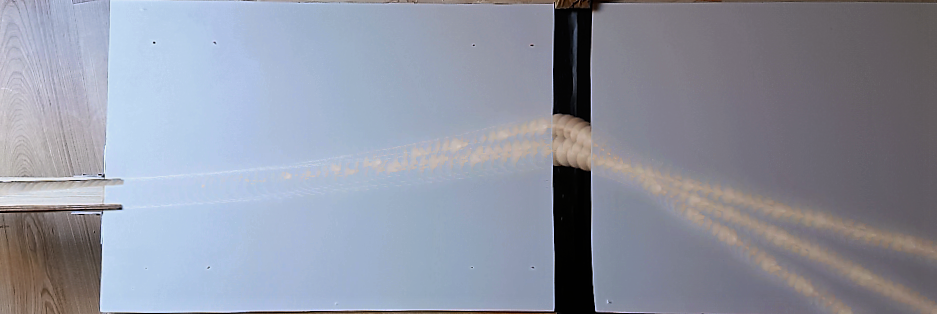
\includegraphics[width=0.99\textwidth]{images/aufbau2.png}
  \caption[Stroboskop-Effekt der Kugeln 8--10]{Die Bahnen der Kugeln 8--10 der Messreihe mit Kugeldurchmesser $r=\SI{35}{\milli\metre}$. Die Rampe befindet sich bei $y=\SI{0}{\centi\metre}$, die Düse des Gebläses bei $x=\SI{60}{\centi\metre}$ und $y=\SI{25}{\centi\metre}$.}
  \label{fig:aufbau2}
  \vspace{-0pt}
\end{figure}

\noindent Wie sich bei dem Vergleich mit \textsc{Mais} herausgestellt hat, werden nur gut $\SI{80}{\percent}$ der potentiellen in kinetische Energie umgesetzt. Um zu überprüfen, ob das neue Konzept für eine Beschleunigereinheit dazu in der Lage ist, die Energie signifikant besser umzuwandeln, wird neben den Daten aus Tabelle \ref{tab:energy} eine Messreihe mit der neuen Startvorrichtung aufgezeichnet, um anschließend einen \textit{Zweistichproben-Test} durchzuführen (siehe Abb. \ref{fig:aufbau2}).\footcite[vgl.][S.\,283]{Cramer2008} 

Bei der Messreihe werden $10$ Kugelbahnen (Radius $\SI{17.5}{\milli\metre}$) per Video aufgezeichnet. An der Beschleunigereinheit sind fünf Markierungen angebracht, von denen aus jeweils zwei Kugeln (1 und 6, 2 und 7 etc.) losgelassen werden. Ein Überblick der Messung liefert Tabelle \ref{tab:maisbex1}.

  \thisfloatsetup{
  capbesidewidth=\marginparwidth,
}
\begin{table}[htb]
\centering
%\sffamily,
\small
%\sansmath
\arrayrulecolor{white}
%\setlength{\arrayrulewidth}{2pt}
\vspace{0.2cm}
  \rowcolors{2}{halfgray!15}{halfgray!5}
 \setlength{\extrarowheight}{.00em}
			\begin{tabularx}{0.99\textwidth}{c*{1}{>{\RaggedLeft\arraybackslash}X}r*{2}{>{\RaggedLeft\arraybackslash}X}}		
\rowcolor{mycolor}  
\multicolumn{1}{c}{\color{white}\textbf{Kugel}} & 
\multicolumn{1}{c}{\color{white}\textbf{Höhe $\boldsymbol{h}$}} &
 \multicolumn{1}{c}{\color{white}\textbf{$\boldsymbol{E_\mathrm{pot}}$ in}} &  \multicolumn{1}{c}{\color{white}\textbf{$\boldsymbol{E_\mathrm{kin}}$ in}} &    \multicolumn{1}{c}{\color{white}\textbf{Abweichung}}\\ \rowcolor{mycolor}
 \multicolumn{1}{c}{\color{white}\textbf{Nr.}} & 
 \multicolumn{1}{c}{\color{white}\textbf{in $\boldsymbol{\si{\milli\metre}}$}} &
     \multicolumn{1}{c}{\color{white}\textbf{$\boldsymbol{\si{\milli\newton\metre}}$}}  &    \multicolumn{1}{c}{\color{white}\textbf{$\boldsymbol{\si{\milli\newton\metre}}$}}  &     \multicolumn{1}{c}{\color{white}\textbf{in $\si{\percent}$}}\\
1	&	22	&	3,392	&	3,050	&	10,1	\\
2	&	24	&	3,700	&	3,398	&	8,2	\\
3	&	35	&	5,396	&	5,242	&	2,8	\\
4	&	47	&	7,245	&	6,922	&	4,5	\\
5	&	60	&	9,250	&	8,813	&	4,7	\\
6	&	22	&	3,392	&	2,915	&	14,0	\\
7	&	24	&	3,700	&	3,398	&	8,2	\\
8	&	35	&	5,396	&	4,930	&	8,6	\\
9	&	47	&	7,245	&	6,706	&	7,4	\\
10	&	60	&	9,250	&	7,517	&	18,7	\\
		\end{tabularx}
		\caption[Umsetzung der potentiellen in kinetische Energie II]{Videoanalyse einer Messreihe mit Holzkugeln des Radius $r=\SI{17.5}{\milli\metre}$. Es werden die ersten $\SI{0.2}{\second}$ zur Berechnung der kinetischen Energie verwendet.}
		\label{tab:maisbex1}	
		\end{table} %\vspace*{-5cm}\newpage

\noindent Seien die beiden unabhängigen Stichproben normalverteilt mit dem Erwartungswert $\mu$ und der Varianz $\sigma^2$, d.\,h.
\begin{equation*}
X_1,...\,,X_{n_1}\distras{iid} N(\mu_1,\, \sigma^2),\,Y_1,\,,Y_{n_2}\distras{iid} Y(\mu_2,\, \sigma^2),
\end{equation*}
wobei angenommen wird, dass die Varianzen gleich sind, da die jeweiligen Startvorrichtungen aus dem gleichen Material erstellt wurden, so ergibt sich der Schätzer für die Varianz zu
\begin{equation*}
\widehat{\sigma}^2=\frac{1}{n_1+n_2-2}\left(\sum\limits_{i=1}^{n_1}(X_i-\overline{X})^2+\sum\limits_{j=1}^{n_2}(Y_j-\overline{Y})^2\right)\approx 18,49
\end{equation*}
Überprüft wird nun die \textit{Teststatistik} $\widehat{D}$
\begin{equation*}
=\frac{\overline{X}-\overline{Y}}{\widehat{\sigma}\sqrt{\sfrac{1}{n_1}+\sfrac{1}{n_2}}}\approx -6,84
\end{equation*}
mit der Entscheidungsregel \textit{die Nullhypothese $H_0: \mu_1\geq \mu_2$ wird abgelehnt, falls}
\begin{equation*}
\widehat{D}<-t_{1-\alpha}(n_1+n_2-2)
\end{equation*}
gilt, wobei $t_{1-\alpha}$ das Beta-Quantil der T-Verteilung ist \footnote{$\beta = 1-\alpha$}. Mit
\begin{equation*}
-t_{0,9995}(17)=-3,965 > \widehat{D}
\end{equation*}
kann zum Signifikanzniveau $\SI{99.95}{\percent}$ bewiesen werden, dass der Erwartungswert der Abweichung zwischen potentieller und kinetischer Energie geringer als bei der alten Startvorrichtung ist. 

Die Messungen der größten Holzkugeln haben im Mittel eine Umsetzung von $\SI{93}{\percent}$ der Lageenergie in kinetische Energie ergeben. Daher wird
das Funktionsprinzip der neuen Startvorrichtung als überlegen angesehen,
bei der mathematischen Beschreibung der Bewegungsgleichung $0,9\cdot E_\mathrm{pot}\approx \sfrac{7}{10}mv^2$ gesetzt und schließlich
vorgeschlagen, diese Beschleunigereinheit von der mechanischen Werkstatt anfertigen zu lassen. 

\section{Voraussagbarkeit}
\label{sec:voraus}
Im Zuge der Planung des Versuchsaufbaus wurde das erwartete Verhalten von Kugeln modelliert. Mit der im vorigen Abschnitt beschriebenen Messreihe wird nun überprüft, inwiefern das Modell Gültigkeit besitzt.

Für den Einfluss der schiefen Ebene werden die in Kapitel \ref{kap:4} aufgestellten Bewegungsgleichungen für die $x$- und $y$-Positionen der rollenden Massen verwendet. Die Krafteinwirkung des Strömungsfeldes wird zunächst als punktueller Kraftstoß angenommen, der eine Geschwindigkeitsänderung in $y$-Richtung verursacht. Damit ergeben sich die graphischen Auftragungen in Abbildung \ref{fig:plot1}

  \thisfloatsetup{%
  capbesidewidth=\marginparwidth}

\begin{figure}[htbp]
\centering
%\sansmath
\begin{tikzpicture}
\begin{axis}[	
	clip=false, % Verhindet weiße Punkte bei vielfach geplotteten x-Werten
	ymajorgrids,
    xmajorgrids,
          axis x line*=middle,
          axis y line*=center,
    grid style={white},
	axis on top,
    width=12cm,
    height=7.797cm,
    xmin=0,
    xmax=1200,
    ymin=-150,
    ymax=200,
    %/tikz/ybar interval,
    tick align=center,
    xtick align=outside,
    xlabel={$x$},
    ylabel={\rotatebox[origin=b]{270}{$y$}},   
   x label style={at={(axis cs:1000,-45)}},
    y label style={at={(axis cs:-150.5,150)}},
    axis line style={Honeydew4!70!black},
    ticklabel style={Honeydew4!70!black, inner sep=1pt,
                font=\footnotesize},
    yticklabels={${-150}$, ${-100}$, ${-50}$,  ${0}$,   ${50}$ , ${100}$, ${\si{\milli\newton}}$, ${200}$ },            
    xtick={200,400,600,800,1000, 1200},
    xticklabels={${200}$, ${400}$, ${600}$,  ${800}$, ${\si{\milli\metre}}$, ${1200}$},
     ytick={-150, -100, -50, 0, 50, 100,150,200 }, 
    scaled ticks=false,
    width=\textwidth,        
       legend style ={ at={(axis cs:150,-30)}, 
         anchor=north west, draw=none, 
             fill=none,align=left, text=Honeydew4!70!black,
              font=\footnotesize},                      
    cycle list name=mycolor4 white,                    
    label style={font=\small,Honeydew4!70!black,},
    enlarge x limits=true,
    %tick style={draw=none},
    x tick label as interval=false,
]
\draw[thick, Honeydew4!70!black, ->,>={latex[Honeydew4!70!black, round, length=0.4cm, width=4pt]}] (axis cs:-150.50, 110) -- (axis cs:-150.50, 190);
\draw[thick,Honeydew4!70!black, ->,>={latex[Honeydew4!70!black,round, length=0.4cm, width=4pt]}] (axis cs:900.00, -45) -- (axis cs:1100.00, -45);
\draw[thick, mycolor!50, fill=mycolor] (axis cs:675,18) circle (3pt);
\addplot
table[x = x, y =y]{images/data/10.dat};
\addlegendentry{$\SI{22.0}{\milli\metre}$};
\addplot
table[x = x, y =y]{images/data/11.dat};
\addlegendentry{$\SI{24.0}{\milli\metre}$};
\addplot
table[x = x, y =y]{images/data/12.dat};
\addlegendentry{$\SI{35.0}{\milli\metre}$};
\addplot
table[x = x, y =y]{images/data/13.dat};
\addlegendentry{$\SI{47.0}{\milli\metre}$};
\addplot
table[x = x, y =y]{images/data/14.dat};
\addlegendentry{$\SI{60.0}{\milli\metre}$};
\end{axis}
\clipright
\end{tikzpicture}
  \caption[Plot der theoretisch berechneten Kugelbahnen]{Plots der theoretisch berechneten Kugelbahnen für Starthöhen $h$, die mit denjenigen der Videoanalysen nahezu übereinstimmen. Der blaue Kreis deutet die approximative Fokussierungszone an (bei $(x,y)\tran = [(675, 19)\tran \pm (10 , 2)\tran] \si{\milli\metre}$).}
  \label{fig:plot1}
  \vspace{-0pt}
\end{figure}
  \thisfloatsetup{%
  capbesidewidth=\marginparwidth}

\begin{figure}[h!tb!p]
\centering
%\sansmath
\begin{tikzpicture}
\begin{axis}[	
	clip=false, % Verhindet weiße Punkte bei vielfach geplotteten x-Werten
	ymajorgrids,
    xmajorgrids,
          axis x line*=middle,
          axis y line*=center,
    grid style={white},
	axis on top,
    width=12cm,
    height=7.797cm,
    xmin=0,
    xmax=1200,
    ymin=-150,
    ymax=200,
    %/tikz/ybar interval,
    tick align=center,
    xtick align=outside,
    xlabel={$x$},
    ylabel={\rotatebox[origin=b]{270}{$y$}},   
   x label style={at={(axis cs:1000,-45)}},
    y label style={at={(axis cs:-150.5,150)}},
    axis line style={Honeydew4!70!black},
    ticklabel style={Honeydew4!70!black, inner sep=1pt,
                font=\footnotesize},
    yticklabels={${-150}$, ${-100}$, ${-50}$,  ${0}$,   ${50}$ , ${100}$, ${\si{\milli\newton}}$, ${200}$ },            
    xtick={200,400,600,800,1000, 1200},
    xticklabels={${200}$, ${400}$, ${600}$,  ${800}$, ${\si{\milli\metre}}$, ${1200}$},
     ytick={-150, -100, -50, 0, 50, 100,150,200 }, 
    scaled ticks=false,
    width=\textwidth,        
       legend style ={ at={(axis cs:150,-30)}, 
         anchor=north west, draw=none, 
             fill=none,align=left, text=Honeydew4!70!black,
              font=\footnotesize},                      
    cycle list name=mycolor4 black,                    
    label style={font=\small,Honeydew4!70!black,},
    enlarge x limits=true,
    %tick style={draw=none},
    x tick label as interval=false,
]
\draw[thick, Honeydew4!70!black, ->,>={latex[Honeydew4!70!black, round, length=0.4cm, width=4pt]}] (axis cs:-150.50, 110) -- (axis cs:-150.50, 190);
\draw[thick,Honeydew4!70!black, ->,>={latex[Honeydew4!70!black,round, length=0.4cm, width=4pt]}] (axis cs:900.00, -45) -- (axis cs:1100.00, -45);
\draw[thick, mycolor!50, fill=mycolor] (axis cs:700,20) circle (6pt);
\addplot
table[x = x, y =y]{images/data/15.dat};
\addlegendentry{$\SI{22.0}{\milli\metre}$};
\addplot
table[x = x, y =y]{images/data/16.dat};
\addlegendentry{$\SI{24.0}{\milli\metre}$};
\addplot
table[x = x, y =y]{images/data/17.dat};
\addlegendentry{$\SI{35.0}{\milli\metre}$};
\addplot
table[x = x, y =y]{images/data/18.dat};
\addlegendentry{$\SI{47.0}{\milli\metre}$};
\addplot
table[x = x, y =y]{images/data/19.dat};
\addlegendentry{$\SI{60.0}{\milli\metre}$};
\end{axis}
\clipright
\end{tikzpicture}
  \caption[Plot der gemessenen Kugelbahnen]{Plots der gemessenen Kugelbahnen für die Massen 6--10 mit den Starthöhen $h_i$. Der blaue Kreis deutet die ungefähre Fokussierungszone an (bei $(x,y)\tran = [(700, 20)\tran \pm (20 , 4)\tran] \si{\milli\metre}$).}
  \label{fig:plot2}
  \vspace{-40pt}
\end{figure}
\newpage

\noindent Die Kugeln 6--10 sind in Abbildung \ref{fig:plot2} aufgetragen. Die Fokussierungs-Zone liegt ca. $\SI{2.5}{\centi\metre}$ weiter als es bei den rechnerischen Werten der Fall ist, was sich mit den Erwartungen deckt: Die Impulsänderung erfolgt nach der Modellierung über eine Strecke von $\SI{6}{\centi\metre}$, d.\,h. drei Zentimeter vor $x=\SI{60}{\centi\metre}$ und drei dahinter. Über diese Distanz werden die Kugeln auf eine Kreisbahn gezwungen, wie dies auch im magnetischen Feld der Fall ist. Je schneller die Kugel, desto größer der Radius. Dadurch verschiebt sich die Spur der Kugeln im Mittel um die halbe Strecke des Kraftstoßes, d.\,h.  $\sfrac{6}{2}\,\si{\centi\metre}=\SI{3}{\centi\metre}$.

Die weiteren Messreihen mit Holzkugeln haben ähnliche, jedoch nicht so gute Ergebnisse geliefert. Die Fokussierung erfolgte jeweils im Bereich von $y=\SI{2}{\centi\metre}$ bis $\SI{5}{\centi\metre}$, wobei es zu mehr Fehlmessungen gekommen ist, die durch die Asymmetrie der Kugeln, mangelhafte Justierung der Startrampe und ein Hüpfen an dem Übergang zwischen den beiden Platten bedingt waren. Die Glasmurmeln lieferten keine akzeptablen Ergebnisse.

Bei dem endgültigen Versuchsaufbau sollten die Übergänge bis zu $\SI{5}{\centi\metre}$ abgeklebt werden, um die Höhendifferenz mit Acryl auszugleichen. Nach einer Antrockenzeit von einigen Stunden kann der gesamte Experimentiertisch beispielsweise mit Klavierlack ausgerollt werden, was den zusätzlichen Vorteil einer größeren Oberflächenhärte liefert, was den Rollwiderstand reduziert.

Die Verlässlichkeit ließe sich weiter erhöhen, indem industriell gefertigte Kugeln in Kugellagerqualität beschafft werden würden. Für einen Versuchsnachmittag sollte ein vollständiger Satz genügen.
\chapter{Schlussbemerkungen}
\label{kap:6}
\bookmarksetupnext{level=paragraph}
\chapterinfo{Mittels der experimentell gewonnenen Daten wird ein mögliches Grobkonzept für einen Praktikumsversuch nebst möglicher Lernziele vorgestellt, worauf ein persönliches Fazit dieser Examensarbeit folgt.}

\textit{Mittels der experimentell gewonnenen Daten wird ein mögliches Grobkonzept für einen Praktikumsversuch nebst möglicher Lernziele vorgestellt, worauf ein persönliches Fazit dieser Examensarbeit folgt}

\section{Versuchskonzept}

Um einen motivierenden Analogieversuch durchführen zu können, wäre es vorteilhaft, alle Kugelarten gleich einzufärben, damit sie nur haptisch unterschieden werden können. Bei einer Benutzung von beispielsweise unlackierten Aluminium- und Acrylkugeln könnte bei den Studierenden ein Akzeptanzproblem der Analogie auftreten, da man im Regelfall bei der Massenspektrometrie vor der Untersuchung auch nicht weiß, wie der Ausgang sein wird.

Werden vier Kugelradien und -arten genutzt, ergibt sich die Möglichkeit, mindestens zwei Dichte-Radius-Kombinationen einzusetzen, die das gleiche Masse-Projektionsfläche-Verhältnis (bzw. im Primärbereich das gleiche $\sfrac{q}{m}$-Verhältnis) aufweisen. Dieses ungleiche Paar kann als Einstieg --- nachdem die Kugeln herumgereicht worden sind --- analysiert werden. Das spürbar unterscheidbare Gewicht in Verbindung mit der gleichen Aufspaltung führt zu einem \textit{kognitiven Konflikt}, der zu den wichtigsten Hilfsmitteln für motivierende Einstiege und langfristiges Behalten zählt. 

Dabei soll darauf geachtet werden, die Kugeln von der gleichen Höhe abzurollen, da anschließend zwei nicht von den Studierenden ertastete Kugeln gleichen Gewichts heruntergerollt werden, woran eine kurze Diskussion anschließen kann. 

Die eigentliche Durchführung des Versuches bietet mannigfaltige Herangehensweisen. Es wäre selbst eine Videoanalyse durchführbar, die jedoch stark reduziert sein müsste: Im Praktikumsversuch \textsc{VID} des I. Physikalischen Instituts der RWTH Aachen wird lediglich ein einziges Video aufgezeichnet und ausgewertet, jedoch füllt der Versuch nichtsdestotrotz einen halben Nachmittag. Im Vordergrund muss stets die Analyse von Probensubstanzen stehen. Ob einzelne \textit{Elemente}, oder eine durchmischte Probe untersucht werden, unterscheidet sich allerdings nur im Schwierigkeitsgrad. 

Auf Grundlage eines Lernzielkatalogs kann eine genaue Passung der Versuchsanleitung und -aufgaben erfolgen. Differenziert nach Studiengängen kann das Anforderungsniveau flexibel angepasst werden. Im Bereich der Zielebenen werden folgende Lernziele vorgeschlagen:
\begin{items}
\item Wie bei den meisten Gruppenversuchen können als \textsw{Leitziele} das heu{\-}ris{\-}tisch-problemlösende Denken und die Fähigkeit zur konstruktiven Gruppenarbeit gesehen werden. Insbesondere das Problemlösen als höchstes Anforderungsniveau kann durch einen Analogieversuch zu einem geschwindigkeitsfokussierenden Massenspektrometer geschult werden. Wird lediglich die Näherungsfunktion des Strömungsfeldes nach Kapitel \ref{kap:5} bei der Forderung nach einer vollständigen Analyse der $\sfrac{q}{m}$-Verhältnisse inklusive Betrachtung der Messungenauigkeiten angegeben, könnten jedoch auch einige Studenten schnell demotiviert werden und nicht weiter am Versuchsgeschehen teilnehmen.
\item Anknüpfend an die Leitziele kann das Übertragen des Analogmodells auf den Lernbereich \textit{Massenspektrometrie} als gehobenes \textsw{Richtziel} gesehen werden. Da die Massenanalyse so viele physikalische Gesetze vereint und kombiniert, stellt ihr Verständnis ebenfalls ein Richtziel dar. Weiterhin gehören auch das experimentelle Arbeiten und Modellieren von Zusammenhängen in diesen Zielbereich. 
\item \textsc{Kircher} betont, dass \textsw{Feinziele} lediglich in der Lehrerausbildung einen begrifflichen Wert haben, da die Operatoren wie \textit{Verstehen} ohne Lerngruppenanalyse nicht auf ihre Erfüllung hin beurteilt werden können.\footcite[vgl.][S\,86]{Kircher2013}
\item Die \textsw{Grobziele}, welche bei der Auseinandersetzung mit dem hier beschriebenen Funktionsmodell verfolgt werden können, sind vielfältig. Neben den Gravitationskraft und den Strömungsfeldern des Analogiebereiches muss die Theorie der Wirkungsweise von elektrischen und magnetischen Feldern wiederholt werden. Die Verbindung dieser Bereiche über Isomorphie-Betrachtungen wie beispielsweise
\begin{equation*}
qU_\mathrm{B}\cong mgh
\end{equation*}
führt zu einer Vernetzung von Wissen und damit zu einem erleichterten Übergang in das Langzeitgedächtnis.
\end{items}
Die Erweiterung des Funktionsmodell um einen Geschwindigkeitsfilter bringt zwar Schwierigkeiten in der Kalibration mit sich, bietet jedoch großes Lernpotential und verschiebt den Versuch auf der mathematisch-naturwissenschaftlichen Skala etwas weiter in Richtung der \textit{Physik}.\vspace*{-1.5cm}\footcite[vgl.][, dessen Konzeption aufgrund der Limitationen des vorigen Analogiemodells eher auf die \textsw{Stochastik} ausgerichtet war. (S.\,48--49)]{Mais2014}\vspace*{1.5cm}

\section{Fazit}

Da die Massenspektrometrie eine in seiner Bedeutung herausstechende Analysemethode für die (Sport-)medizin, Naturwissenschaften und Industrie  darstellt, wurde im Zuge dieser Hausarbeit der Versuch unternommen, ein geschwindigkeitsfokussierendes Funktionsmodell zu entwickeln, das auch abseits von Demonstrationsexperimenten und qualitativen Schülerversuchen eingesetzt werden kann. Physikstudenten sollte zwar die Möglichkeit eingeräumt werden, an einem aktualem Massenspektrometer experimentieren zu dürfen, jedoch ist es sowohl aus Gründen des Fachwissens als auch der Interessen für Nebenfachstudierende sinnvoller --- zumindest zu Beginn --- das Funktionsprinzip an einem Analogiemodell zu erarbeiten.

Die hier vorgeschlagene Analogie erfüllt die beiden Kriterien nach \textsc{Kircher}: Der Modellversuch und \textsc{Aston}s Massenspektrometer sind in der Bewegungsbeschreibung der Teilchen \textit{oberflächenähnlich}, die Begriffe und Objekte von Primär- und Sekundärbereich sind weitestgehend \textit{isomorph}. Die Unzulänglichkeiten von Analogiemodellen sollen in einem Praktikumsversuch hingegen nicht erörtert werden.\footcite[vgl.][S.\,128--129]{Kircher2013}  

Es konnte jedem Objekt des primären Lernbereichs im Analogieversuch begrifflich-mathematisch eine Entsprechung zugewiesen werden. Insbesondere die Energieerhaltung, Bewegungsgleichungen im Coulomb-Feld, die Impulsänderung beim Passieren eines Magnetfeldes, Masse und Ladung finden ihre Entsprechungen im entwickelten Versuchsaufbau.

Die ausgewählten Ähnlichkeitsbeziehungen konnten experimentell bestätigt werden, obwohl die Ungenauigkeit der selbstgebauten Startrampe und besonders der Holz- und Glaskugeln dazu beigetragen haben, dass eine große Menge an Messdaten durch Fehlmessungen immer weiter abgeschmolzen wurde. 

Bei einer professionell gefertigten Ausführung liegt ein enormes Wertschöpfungspotential in dem vorgestellten Funktionsmodell, das --- meines Wissens --- das Erste ist, welches Impuls- und Energieanalyse, Massen- und Ladungsanalogien miteinander vereint. Diese Menge an Parametern, die bildlich als Stellschrauben gesehen werden können, führte dazu, dass ständig Komponenten verändert werden mussten. Obwohl ich um das frühe Stadium des Prototypen weiß, bin ich überzeugt, dass der Versuch \textsc{MAS} in naher Zukunft seinen Platz in den physikalischen Praktika für Nebenfachstudierende finden wird.





%%% -- end of main content

% -- bibliography --
% (must be placed _before_ appendix)
\boldPDFchaptersfalse

% Biblatex Zeilenumbrpüche manuell mittels {\-}

\IfPackageLoaded{biblatex}{
  \cleardoublepage
  \IfDefined{phantomsection}{\phantomsection}\label{sec:bibliography}
  \printbibliography[
  	%env=numbered+bold
   % heading=bibintoc,
    title = {Literaturverzeichnis}
 % (bibintoc, bibnumbered)
  ]	
\addcontentsline{toc}{chapter}{\protect\lowercase\protect\texorpdfstring{{ %\color{mycolor} 
\protect\hspace*{-0.1cm}Literaturverzeichnis}}{Literaturverzeichnis}}
  }% end of bibliography
  \newpage
\pagenumbering{roman}
\setcounter{page}{3}
%% -- list of figures and tables --

\cleardoublepage\IfDefined{phantomsection}{\phantomsection}\label{sec:lof}
\listoffigures
\cleardoublepage\IfDefined{phantomsection}{\phantomsection}\label{sec:lot}
\listoftables

%% -- List of Listings --
% _Remove_ if no listing with caption is defined
%\cleardoublepage
%\IfDefined{lstlistoflistings}{\cleardoublepage\lstlistoflistings}
%\addcontentsline{toc}{section}{Quellcode}

% --- Appendix --- --- --- --- --- --- ---
 \cleardoublepage
\cleardoublepage\IfDefined{phantomsection}{\phantomsection}
\appendix
% Add `Appendix` to TOC
%\addcontentsline{toc}{part}{III \appendixname}
% must be _input_, otherwise the TOC entry is at the wrong place
\startcontents
\chapter{Messdaten}




\stopcontents
\section{Tabellen}

  \thisfloatsetup{
   capposition=top,
}
\begin{table}[htb]
\centering
%\sffamily,
\small
%\sansmath
\arrayrulecolor{white}
%\setlength{\arrayrulewidth}{2pt}
\vspace{0.2cm}
  \rowcolors{2}{halfgray!15}{halfgray!5}
 \setlength{\extrarowheight}{.00em}
			\begin{tabularx}{0.99\fulllinewidth}{*{2}{>{\RaggedLeft\arraybackslash}X}X*{3}{>{\RaggedLeft\arraybackslash}X}}	
\rowcolor{mycolor}  {\color{white}\textbf{ Radius $\boldsymbol{r}$ in $\boldsymbol{\si{\milli\metre}}$}} & {\color{white}\textbf{Abstand $\boldsymbol{s}$ in $\boldsymbol{\si{\centi\metre}}$}} & {\color{white}\textbf{Amplitude $\boldsymbol{A}$ in $\boldsymbol{\si{\milli\newton}}$}} & {\color{white}\textbf{$\boldsymbol{\mu}$}} & {\color{white}\textbf{$\boldsymbol{2\sigma^2}$}}& {\color{white}\textbf{$\boldsymbol{R^2}$}}\\
	&	1	&	188,1	&	2,133	&	-0,230	&	0,990	\\
	&	5	&	165,1	&	1,962	&	-0,123	&	0,991	\\
	&	10	&	125,7	&	2,092	&	-0,679	&	0,992	\\
	&	15	&	80,2	&	2,141	&	-0,533	&	0,994	\\
	&	20	&	72,7	&	2,743	&	-1,408	&	0,991	\\
	&	25	&	59,2	&	3,421	&	-0,612	&	0,992	\\
\multirow{-7}{*}{17,5}	&	30	&	42,7	&	3,499	&	-0,931	&	0,975	\\
	&	1	&	143,4	&	1,929	&	-0,367	&	0,996	\\
	&	5	&	117,9	&	1,836	&	-0,615	&	0,994	\\
	&	10	&	84,3	&	2,067	&	-0,690	&	0,990	\\
	&	15	&	64,6	&	2,338	&	-0,452	&	0,995	\\
	&	20	&	50,3	&	2,392	&	-0,608	&	0,985	\\
	&	25	&	39,9	&	3,051	&	-1,257	&	0,991	\\
\multirow{-7}{*}{15,0}	&	30	&	34,2	&	3,831	&	-1,841	&	0,973	\\
	&	1	&	101,2	&	1,832	&	-0,526	&	0,993	\\
	&	5	&	87,6	&	1,805	&	-0,617	&	0,991	\\
	&	10	&	61,8	&	2,019	&	-0,769	&	0,992	\\
	&	15	&	45,8	&	2,291	&	-1,138	&	0,997	\\
	&	20	&	37,3	&	2,796	&	-1,119	&	0,993	\\
	&	25	&	30,4	&	2,933	&	-1,923	&	0,993	\\
\multirow{-7}{*}{12,5}	&	30	&	22,7	&	3,844	&	-1,802	&	0,981	\\
	&	1	&	65,6	&	1,752	&	-0,612	&	0,993	\\
	&	5	&	51,5	&	1,530	&	-0,777	&	0,994	\\
	&	10	&	37,9	&	1,612	&	-0,711	&	0,997	\\
	&	15	&	27,5	&	1,540	&	-0,852	&	0,979	\\
	&	20	&	23,4	&	2,309	&	-1,025	&	0,993	\\
	&	25	&	17,7	&	2,412	&	-1,380	&	0,991	\\
\multirow{-7}{*}{10,0}	&	30	&	13,7	&	2,679	&	-2,120	&	0,981	\\
		\end{tabularx}
		\caption[Ergebnisse der Gaußanpassungen für die niedrigere Gebläsestufe]{Ergebnisse der Gaußanpassungen für die niedrigere Gebläsestufe.}
		\label{tab:gaaussfit2}	
		\end{table} %\vspace*{-5cm}\newpage
  \thisfloatsetup{
  capposition=bottom,
}
\begin{table*}
\centering
%\sffamily,
\footnotesize
%\sansmath
\arrayrulecolor{white}
%\setlength{\arrayrulewidth}{2pt}
\vspace{0.2cm}
  \rowcolors{2}{halfgray!15}{halfgray!5}
 \setlength{\extrarowheight}{.00em}
 \subfloat[$s=\SI{10}{\centi\metre}$]{
			\begin{tabularx}{0.30\fulllinewidth}{r*{2}{>{\RaggedLeft\arraybackslash}X}}	
\rowcolor{mycolor} & 	\multicolumn{2}{c}{{\color{white}\textbf{Kraft in $\boldsymbol{\si{\milli\newton}}$}}} \\
\rowcolor{mycolor}  \multirow{-2}{*}{{\color{white}\textbf{$\boldsymbol{d}$ in $\boldsymbol{\si{\centi\metre}}$}}} & \multicolumn{1}{c}{{\color{white}\textbf{Stufe 2}}} &\multicolumn{1}{c}{{\color{white}\textbf{Stufe 1}}}\\
-5,5	$\pm$	0,3	&	0	&	0	\\
-5,0	$\pm$	0,3	&	0	&	0	\\
-4,5	$\pm$	0,3	&	0	&	0	\\
-4,0	$\pm$	0,3	&	5	&	2	\\
-3,5	$\pm$	0,3	&	23	&	9	\\
-3,0	$\pm$	0,3	&	59	&	39	\\
-2,5	$\pm$	0,3	&	87	&	67	\\
-2,0	$\pm$	0,3	&	125	&	89	\\
-1,5	$\pm$	0,3	&	150	&	108	\\
-1,0	$\pm$	0,3	&	168	&	119	\\
-0,5	$\pm$	0,3	&	181	&	119	\\
0,0	$\pm$	0,3	&	175	&	115	\\
0,5	$\pm$	0,3	&	159	&	91	\\
1,0	$\pm$	0,3	&	130	&	72	\\
1,5	$\pm$	0,3	&	100	&	43	\\
2,0	$\pm$	0,3	&	81	&	25	\\
2,5	$\pm$	0,3	&	43	&	8	\\
3,0	$\pm$	0,3	&	20	&	2	\\
3,5	$\pm$	0,3	&	7	&	0	\\
4,0	$\pm$	0,3	&	0	&	0	\\
4,5	$\pm$	0,3	&	0	&	0	\\
		\end{tabularx}}
		\quad
 \subfloat[$s=\SI{15}{\centi\metre}$]{
			\begin{tabularx}{0.30\fulllinewidth}{r*{2}{>{\RaggedLeft\arraybackslash}X}}	
\rowcolor{mycolor} & 	\multicolumn{2}{c}{{\color{white}\textbf{Kraft in $\boldsymbol{\si{\milli\newton}}$}}} \\
\rowcolor{mycolor}  \multirow{-2}{*}{{\color{white}\textbf{$\boldsymbol{d}$ in $\boldsymbol{\si{\centi\metre}}$}}} & \multicolumn{1}{c}{{\color{white}\textbf{Stufe 2}}} &\multicolumn{1}{c}{{\color{white}\textbf{Stufe 1}}}\\
-5,5	$\pm$	0,5	&	0	&	0	\\
-5,0	$\pm$	0,5	&	0	&	0	\\
-4,5	$\pm$	0,5	&	0	&	0	\\
-4,0	$\pm$	0,5	&	6	&	0	\\
-3,5	$\pm$	0,5	&	18	&	8	\\
-3,0	$\pm$	0,5	&	45	&	25	\\
-2,5	$\pm$	0,5	&	65	&	36	\\
-2,0	$\pm$	0,5	&	88	&	48	\\
-1,5	$\pm$	0,5	&	108	&	65	\\
-1,0	$\pm$	0,5	&	133	&	79	\\
-0,5	$\pm$	0,5	&	144	&	82	\\
0,0	$\pm$	0,5	&	153	&	75	\\
0,5	$\pm$	0,5	&	148	&	60	\\
1,0	$\pm$	0,5	&	116	&	45	\\
1,5	$\pm$	0,5	&	93	&	34	\\
2,0	$\pm$	0,5	&	61	&	22	\\
2,5	$\pm$	0,5	&	44	&	15	\\
3,0	$\pm$	0,5	&	22	&	8	\\
3,5	$\pm$	0,5	&	5	&	2	\\
4,0	$\pm$	0,5	&	0	&	0	\\
4,5	$\pm$	0,5	&	0	&	0	\\
		\end{tabularx}}	
		\quad
 \subfloat[$s=\SI{20}{\centi\metre}$]{
			\begin{tabularx}{0.3\fulllinewidth}{r*{2}{>{\RaggedLeft\arraybackslash}X}}	
\rowcolor{mycolor} & 	\multicolumn{2}{c}{{\color{white}\textbf{Kraft in $\boldsymbol{\si{\milli\newton}}$}}} \\
\rowcolor{mycolor}  \multirow{-2}{*}{{\color{white}\textbf{$\boldsymbol{d}$ in $\boldsymbol{\si{\centi\metre}}$}}} & \multicolumn{1}{c}{{\color{white}\textbf{Stufe 2}}} &\multicolumn{1}{c}{{\color{white}\textbf{Stufe 1}}}\\
-5,5	$\pm$	0,7	&	3	&	8	\\
-5,0	$\pm$	0,7	&	5	&	15	\\
-4,5	$\pm$	0,7	&	7	&	23	\\
-4,0	$\pm$	0,7	&	15	&	32	\\
-3,5	$\pm$	0,7	&	29	&	42	\\
-3,0	$\pm$	0,7	&	46	&	52	\\
-2,5	$\pm$	0,7	&	59	&	60	\\
-2,0	$\pm$	0,7	&	85	&	64	\\
-1,5	$\pm$	0,7	&	108	&	70	\\
-1,0	$\pm$	0,7	&	118	&	75	\\
-0,5	$\pm$	0,7	&	120	&	70	\\
0,0	$\pm$	0,7	&	116	&	60	\\
0,5	$\pm$	0,7	&	108	&	41	\\
1,0	$\pm$	0,7	&	86	&	30	\\
1,5	$\pm$	0,7	&	70	&	23	\\
2,0	$\pm$	0,7	&	56	&	14	\\
2,5	$\pm$	0,7	&	40	&	10	\\
3,0	$\pm$	0,7	&	23	&	7	\\
3,5	$\pm$	0,7	&	13	&	5	\\
4,0	$\pm$	0,7	&	6	&	0	\\
4,5	$\pm$	0,7	&	3	&	0	\\
		\end{tabularx}}		
		\\
 \subfloat[$s=\SI{25}{\centi\metre}$]{
			\begin{tabularx}{0.30\fulllinewidth}{r*{2}{>{\RaggedLeft\arraybackslash}X}}	
\rowcolor{mycolor} & 	\multicolumn{2}{c}{{\color{white}\textbf{Kraft in $\boldsymbol{\si{\milli\newton}}$}}} \\
\rowcolor{mycolor}  \multirow{-2}{*}{{\color{white}\textbf{$\boldsymbol{d}$ in $\boldsymbol{\si{\centi\metre}}$}}} & \multicolumn{1}{c}{{\color{white}\textbf{Stufe 2}}} &\multicolumn{1}{c}{{\color{white}\textbf{Stufe 1}}}\\
-7,0	$\pm$	0,9	&	0	&	0	\\
-6,5	$\pm$	0,9	&	7	&	4	\\
-6,0	$\pm$	0,9	&	16	&	8	\\
-5,5	$\pm$	0,9	&	20	&	10	\\
-5,0	$\pm$	0,9	&	26	&	13	\\
-4,5	$\pm$	0,9	&	31	&	15	\\
-4,0	$\pm$	0,9	&	41	&	21	\\
-3,5	$\pm$	0,9	&	48	&	29	\\
-3,0	$\pm$	0,9	&	55	&	34	\\
-2,5	$\pm$	0,9	&	65	&	42	\\
-2,0	$\pm$	0,9	&	73	&	50	\\
-1,5	$\pm$	0,9	&	84	&	57	\\
-1,0	$\pm$	0,9	&	93	&	60	\\
-0,5	$\pm$	0,9	&	94	&	60	\\
0,0	$\pm$	0,9	&	95	&	60	\\
0,5	$\pm$	0,9	&	93	&	53	\\
1,0	$\pm$	0,9	&	87	&	43	\\
1,5	$\pm$	0,9	&	76	&	38	\\
2,0	$\pm$	0,9	&	60	&	32	\\
2,5	$\pm$	0,9	&	50	&	28	\\
3,0	$\pm$	0,9	&	39	&	22	\\
3,5	$\pm$	0,9	&	30	&	14	\\
4,0	$\pm$	0,9	&	19	&	11	\\
4,5	$\pm$	0,9	&	8	&	7	\\
5,0	$\pm$	0,9	&	5	&	4	\\
5,5	$\pm$	0,9	&	0	&	0	\\
6,0	$\pm$	0,9	&	0	&	0	\\
		\end{tabularx}}
		\quad
 \subfloat[$s=\SI{30}{\centi\metre}$]{
			\begin{tabularx}{0.30\fulllinewidth}{r*{2}{>{\RaggedLeft\arraybackslash}X}}	
\rowcolor{mycolor} & 	\multicolumn{2}{c}{{\color{white}\textbf{Kraft in $\boldsymbol{\si{\milli\newton}}$}}} \\
\rowcolor{mycolor}  \multirow{-2}{*}{{\color{white}\textbf{$\boldsymbol{d}$ in $\boldsymbol{\si{\centi\metre}}$}}} & \multicolumn{1}{c}{{\color{white}\textbf{Stufe 2}}} &\multicolumn{1}{c}{{\color{white}\textbf{Stufe 1}}}\\
-7,0	$\pm$	1,1	&	5	&	1	\\
-6,5	$\pm$	1,1	&	8	&	2	\\
-6,0	$\pm$	1,1	&	12	&	4	\\
-5,5	$\pm$	1,1	&	15	&	10	\\
-5,0	$\pm$	1,1	&	17	&	10	\\
-4,5	$\pm$	1,1	&	20	&	13	\\
-4,0	$\pm$	1,1	&	25	&	17	\\
-3,5	$\pm$	1,1	&	36	&	23	\\
-3,0	$\pm$	1,1	&	43	&	30	\\
-2,5	$\pm$	1,1	&	54	&	37	\\
-2,0	$\pm$	1,1	&	64	&	42	\\
-1,5	$\pm$	1,1	&	71	&	45	\\
-1,0	$\pm$	1,1	&	75	&	45	\\
-0,5	$\pm$	1,1	&	76	&	43	\\
0,0	$\pm$	1,1	&	70	&	37	\\
0,5	$\pm$	1,1	&	65	&	30	\\
1,0	$\pm$	1,1	&	56	&	27	\\
1,5	$\pm$	1,1	&	51	&	26	\\
2,0	$\pm$	1,1	&	42	&	23	\\
2,5	$\pm$	1,1	&	32	&	20	\\
3,0	$\pm$	1,1	&	26	&	15	\\
3,5	$\pm$	1,1	&	20	&	9	\\
4,0	$\pm$	1,1	&	12	&	7	\\
4,5	$\pm$	1,1	&	10	&	5	\\
5,0	$\pm$	1,1	&	5	&	4	\\
5,5	$\pm$	1,1	&	4	&	3	\\
6,0	$\pm$	1,1	&	4	&	2	\\
		\end{tabularx}}					
		\caption[Kraftmessung des Gebläses. Kugelradius $r=\SI{17.5}{\milli\metre}$, $s=\SI{10}{\centi\metre}$ bis $\SI{30}{\centi\metre}$]{Kraftmessung des Gebläses. Kugelradius $r=\SI{17.5}{\milli\metre}$, $d=\SI{10}{\centi\metre}$ bis $\SI{30}{\centi\metre}$} 
		\label{tab:kraftmessung2}	
		\end{table*} \vspace*{-5cm}
  \thisfloatsetup{
  capposition=bottom,
}
\begin{table*}
\centering
%\sffamily,
\small
%\sansmath
\arrayrulecolor{white}
%\setlength{\arrayrulewidth}{2pt}
\vspace{0.2cm}
  \rowcolors{2}{halfgray!15}{halfgray!5}
 \setlength{\extrarowheight}{.00em}
 \subfloat[$s=\SI{1}{\centi\metre}$]{
			\begin{tabularx}{0.30\fulllinewidth}{r*{2}{>{\RaggedLeft\arraybackslash}X}}	
\rowcolor{mycolor} & 	\multicolumn{2}{c}{{\color{white}\textbf{Kraft in $\boldsymbol{\si{\milli\newton}}$}}} \\
\rowcolor{mycolor}  \multirow{-2}{*}{{\color{white}\textbf{$\boldsymbol{d}$ in $\boldsymbol{\si{\centi\metre}}$}}} & \multicolumn{1}{c}{{\color{white}\textbf{Stufe 2}}} &\multicolumn{1}{c}{{\color{white}\textbf{Stufe 1}}}\\
-4,5	$\pm$	0,1	&	0	&	0	\\
-4,0	$\pm$	0,1	&	0	&	0	\\
-3,5	$\pm$	0,1	&	4	&	2	\\
-3,0	$\pm$	0,1	&	34	&	24	\\
-2,5	$\pm$	0,1	&	57	&	49	\\
-2,0	$\pm$	0,1	&	105	&	69	\\
-1,5	$\pm$	0,1	&	154	&	99	\\
-1,0	$\pm$	0,1	&	199	&	130	\\
-0,5	$\pm$	0,1	&	222	&	141	\\
0,0	$\pm$	0,1	&	225	&	141	\\
0,5	$\pm$	0,1	&	200	&	117	\\
1,0	$\pm$	0,1	&	149	&	83	\\
1,5	$\pm$	0,1	&	98	&	57	\\
2,0	$\pm$	0,1	&	64	&	39	\\
2,5	$\pm$	0,1	&	19	&	14	\\
3,0	$\pm$	0,1	&	0	&	0	\\
3,5	$\pm$	0,1	&	0	&	0	\\
		\end{tabularx}}
		\quad
 \subfloat[$s=\SI{5}{\centi\metre}$]{
			\begin{tabularx}{0.30\fulllinewidth}{r*{2}{>{\RaggedLeft\arraybackslash}X}}	
\rowcolor{mycolor} & 	\multicolumn{2}{c}{{\color{white}\textbf{Kraft in $\boldsymbol{\si{\milli\newton}}$}}} \\
\rowcolor{mycolor}  \multirow{-2}{*}{{\color{white}\textbf{$\boldsymbol{d}$ in $\boldsymbol{\si{\centi\metre}}$}}} & \multicolumn{1}{c}{{\color{white}\textbf{Stufe 2}}} &\multicolumn{1}{c}{{\color{white}\textbf{Stufe 1}}}\\
-4,5	$\pm$	0,2	&	0	&	0	\\
-4,0	$\pm$	0,2	&	0	&	0	\\
-3,5	$\pm$	0,2	&	2	&	0	\\
-3,0	$\pm$	0,2	&	20	&	18	\\
-2,5	$\pm$	0,2	&	64	&	43	\\
-2,0	$\pm$	0,2	&	119	&	73	\\
-1,5	$\pm$	0,2	&	155	&	95	\\
-1,0	$\pm$	0,2	&	194	&	111	\\
-0,5	$\pm$	0,2	&	193	&	115	\\
0,0	$\pm$	0,2	&	173	&	104	\\
0,5	$\pm$	0,2	&	149	&	81	\\
1,0	$\pm$	0,2	&	115	&	58	\\
1,5	$\pm$	0,2	&	86	&	36	\\
2,0	$\pm$	0,2	&	36	&	14	\\
2,5	$\pm$	0,2	&	6	&	0	\\
3,0	$\pm$	0,2	&	0	&	0	\\
3,5	$\pm$	0,2	&	0	&	0	\\
		\end{tabularx}}	
		\quad
 \subfloat[$s=\SI{10}{\centi\metre}$]{
			\begin{tabularx}{0.3\fulllinewidth}{r*{2}{>{\RaggedLeft\arraybackslash}X}}	
\rowcolor{mycolor} & 	\multicolumn{2}{c}{{\color{white}\textbf{Kraft in $\boldsymbol{\si{\milli\newton}}$}}} \\
\rowcolor{mycolor}  \multirow{-2}{*}{{\color{white}\textbf{$\boldsymbol{d}$ in $\boldsymbol{\si{\centi\metre}}$}}} & \multicolumn{1}{c}{{\color{white}\textbf{Stufe 2}}} &\multicolumn{1}{c}{{\color{white}\textbf{Stufe 1}}}\\
-4,5	$\pm$	0,3	&	0	&	0	\\
-4,0	$\pm$	0,3	&	3	&	0	\\
-3,5	$\pm$	0,3	&	10	&	5	\\
-3,0	$\pm$	0,3	&	44	&	26	\\
-2,5	$\pm$	0,3	&	75	&	44	\\
-2,0	$\pm$	0,3	&	101	&	58	\\
-1,5	$\pm$	0,3	&	117	&	72	\\
-1,0	$\pm$	0,3	&	132	&	83	\\
-0,5	$\pm$	0,3	&	131	&	84	\\
0,0	$\pm$	0,3	&	129	&	69	\\
0,5	$\pm$	0,3	&	116	&	63	\\
1,0	$\pm$	0,3	&	96	&	42	\\
1,5	$\pm$	0,3	&	58	&	33	\\
2,0	$\pm$	0,3	&	37	&	16	\\
2,5	$\pm$	0,3	&	14	&	7	\\
3,0	$\pm$	0,3	&	3	&	2	\\
3,5	$\pm$	0,3	&	0	&	0	\\
		\end{tabularx}}		
		\\
 \subfloat[$s=\SI{15}{\centi\metre}$]{
			\begin{tabularx}{0.30\fulllinewidth}{r*{2}{>{\RaggedLeft\arraybackslash}X}}	
\rowcolor{mycolor} & 	\multicolumn{2}{c}{{\color{white}\textbf{Kraft in $\boldsymbol{\si{\milli\newton}}$}}} \\
\rowcolor{mycolor}  \multirow{-2}{*}{{\color{white}\textbf{$\boldsymbol{d}$ in $\boldsymbol{\si{\centi\metre}}$}}} & \multicolumn{1}{c}{{\color{white}\textbf{Stufe 2}}} &\multicolumn{1}{c}{{\color{white}\textbf{Stufe 1}}}\\
-6,5	$\pm$	0,5	&	0	&	0	\\
-6,0	$\pm$	0,5	&	0	&	0	\\
-5,5	$\pm$	0,5	&	0	&	0	\\
-5,0	$\pm$	0,5	&	0	&	0	\\
-4,5	$\pm$	0,5	&	2	&	0	\\
-4,0	$\pm$	0,5	&	8	&	4	\\
-3,5	$\pm$	0,5	&	19	&	9	\\
-3,0	$\pm$	0,5	&	38	&	19	\\
-2,5	$\pm$	0,5	&	54	&	35	\\
-2,0	$\pm$	0,5	&	69	&	42	\\
-1,5	$\pm$	0,5	&	86	&	53	\\
-1,0	$\pm$	0,5	&	103	&	61	\\
-0,5	$\pm$	0,5	&	104	&	63	\\
0,0	$\pm$	0,5	&	101	&	62	\\
0,5	$\pm$	0,5	&	92	&	53	\\
1,0	$\pm$	0,5	&	76	&	46	\\
1,5	$\pm$	0,5	&	53	&	34	\\
2,0	$\pm$	0,5	&	38	&	20	\\
2,5	$\pm$	0,5	&	22	&	14	\\
3,0	$\pm$	0,5	&	14	&	7	\\
3,5	$\pm$	0,5	&	6	&	4	\\
4,0	$\pm$	0,5	&	0	&	0	\\
4,5	$\pm$	0,5	&	0	&	0	\\
5,0	$\pm$	0,5	&	0	&	0	\\
5,5	$\pm$	0,5	&	0	&	0	\\
		\end{tabularx}}
		\quad
		 \subfloat[$s=\SI{20}{\centi\metre}$]{
					\begin{tabularx}{0.30\fulllinewidth}{r*{2}{>{\RaggedLeft\arraybackslash}X}}	
		\rowcolor{mycolor} & 	\multicolumn{2}{c}{{\color{white}\textbf{Kraft in $\boldsymbol{\si{\milli\newton}}$}}} \\
		\rowcolor{mycolor}  \multirow{-2}{*}{{\color{white}\textbf{$\boldsymbol{d}$ in $\boldsymbol{\si{\centi\metre}}$}}} & \multicolumn{1}{c}{{\color{white}\textbf{Stufe 2}}} &\multicolumn{1}{c}{{\color{white}\textbf{Stufe 1}}}\\
-6,5	$\pm$	0,7	&	0	&	0	\\
-6,0	$\pm$	0,7	&	0	&	0	\\
-5,5	$\pm$	0,7	&	2	&	0	\\
-5,0	$\pm$	0,7	&	4	&	0	\\
-4,5	$\pm$	0,7	&	8	&	2	\\
-4,0	$\pm$	0,7	&	11	&	5	\\
-3,5	$\pm$	0,7	&	21	&	14	\\
-3,0	$\pm$	0,7	&	34	&	28	\\
-2,5	$\pm$	0,7	&	44	&	34	\\
-2,0	$\pm$	0,7	&	54	&	39	\\
-1,5	$\pm$	0,7	&	69	&	46	\\
-1,0	$\pm$	0,7	&	84	&	48	\\
-0,5	$\pm$	0,7	&	84	&	50	\\
0,0	$\pm$	0,7	&	85	&	46	\\
0,5	$\pm$	0,7	&	76	&	42	\\
1,0	$\pm$	0,7	&	64	&	36	\\
1,5	$\pm$	0,7	&	48	&	24	\\
2,0	$\pm$	0,7	&	40	&	21	\\
2,5	$\pm$	0,7	&	26	&	16	\\
3,0	$\pm$	0,7	&	16	&	11	\\
3,5	$\pm$	0,7	&	10	&	6	\\
4,0	$\pm$	0,7	&	4	&	4	\\
4,5	$\pm$	0,7	&	0	&	0	\\
5,0	$\pm$	0,7	&	0	&	0	\\
5,5	$\pm$	0,7	&	0	&	0	\\
				\end{tabularx}}		
				\quad
 \subfloat[$s=\SI{25}{\centi\metre}$]{
			\begin{tabularx}{0.30\fulllinewidth}{r*{2}{>{\RaggedLeft\arraybackslash}X}}	
\rowcolor{mycolor} & 	\multicolumn{2}{c}{{\color{white}\textbf{Kraft in $\boldsymbol{\si{\milli\newton}}$}}} \\
\rowcolor{mycolor}  \multirow{-2}{*}{{\color{white}\textbf{$\boldsymbol{d}$ in $\boldsymbol{\si{\centi\metre}}$}}} & \multicolumn{1}{c}{{\color{white}\textbf{Stufe 2}}} &\multicolumn{1}{c}{{\color{white}\textbf{Stufe 1}}}\\
-6,5	$\pm$	0,9	&	5	&	0	\\
-6,0	$\pm$	0,9	&	4	&	4	\\
-5,5	$\pm$	0,9	&	9	&	4	\\
-5,0	$\pm$	0,9	&	11	&	6	\\
-4,5	$\pm$	0,9	&	20	&	14	\\
-4,0	$\pm$	0,9	&	26	&	18	\\
-3,5	$\pm$	0,9	&	34	&	24	\\
-3,0	$\pm$	0,9	&	36	&	31	\\
-2,5	$\pm$	0,9	&	48	&	34	\\
-2,0	$\pm$	0,9	&	54	&	36	\\
-1,5	$\pm$	0,9	&	63	&	40	\\
-1,0	$\pm$	0,9	&	66	&	39	\\
-0,5	$\pm$	0,9	&	66	&	36	\\
0,0	$\pm$	0,9	&	64	&	36	\\
0,5	$\pm$	0,9	&	57	&	29	\\
1,0	$\pm$	0,9	&	48	&	21	\\
1,5	$\pm$	0,9	&	41	&	16	\\
2,0	$\pm$	0,9	&	32	&	14	\\
2,5	$\pm$	0,9	&	24	&	10	\\
3,0	$\pm$	0,9	&	17	&	6	\\
3,5	$\pm$	0,9	&	12	&	4	\\
4,0	$\pm$	0,9	&	6	&	4	\\
4,5	$\pm$	0,9	&	4	&	2	\\
5,0	$\pm$	0,9	&	2	&	1	\\
5,5	$\pm$	0,9	&	0	&	0	\\
		\end{tabularx}}					
		\caption[Kraftmessung des Gebläses. Kugelradius $r=\SI{15.0}{\milli\metre}$, $s=\SI{1}{\centi\metre}$ bis $\SI{25}{\centi\metre}$]{Kraftmessung des Gebläses. Kugelradius $r=\SI{15.0}{\milli\metre}$, $d=\SI{1}{\centi\metre}$ bis $\SI{25}{\centi\metre}$} 
		\label{tab:kraftmessung3}	
		\end{table*} \vspace*{-5cm}
  \thisfloatsetup{
  capposition=bottom,
}
\begin{table*}
\centering
%\sffamily,
\small
%\sansmath
\arrayrulecolor{white}
%\setlength{\arrayrulewidth}{2pt}
\vspace{0.2cm}
  \rowcolors{2}{halfgray!15}{halfgray!5}
 \setlength{\extrarowheight}{.00em}
 \subfloat[$s=\SI{1}{\centi\metre}$]{
			\begin{tabularx}{0.30\fulllinewidth}{r*{2}{>{\RaggedLeft\arraybackslash}X}}	
\rowcolor{mycolor} & 	\multicolumn{2}{c}{{\color{white}\textbf{Kraft in $\boldsymbol{\si{\milli\newton}}$}}} \\
\rowcolor{mycolor}  \multirow{-2}{*}{{\color{white}\textbf{$\boldsymbol{d}$ in $\boldsymbol{\si{\centi\metre}}$}}} & \multicolumn{1}{c}{{\color{white}\textbf{Stufe 2}}} &\multicolumn{1}{c}{{\color{white}\textbf{Stufe 1}}}\\
-5,0	$\pm$	0,1	&	0	&	0	\\
-4,5	$\pm$	0,1	&	0	&	0	\\
-4,0	$\pm$	0,1	&	0	&	0	\\
-3,5	$\pm$	0,1	&	1	&	2	\\
-3,0	$\pm$	0,1	&	21	&	15	\\
-2,5	$\pm$	0,1	&	56	&	32	\\
-2,0	$\pm$	0,1	&	81	&	51	\\
-1,5	$\pm$	0,1	&	119	&	78	\\
-1,0	$\pm$	0,1	&	149	&	100	\\
-0,5	$\pm$	0,1	&	159	&	101	\\
0,0	$\pm$	0,1	&	141	&	86	\\
0,5	$\pm$	0,1	&	116	&	74	\\
1,0	$\pm$	0,1	&	89	&	51	\\
1,5	$\pm$	0,1	&	57	&	34	\\
2,0	$\pm$	0,1	&	32	&	21	\\
2,5	$\pm$	0,1	&	2	&	1	\\
3,0	$\pm$	0,1	&	0	&	0	\\
		\end{tabularx}}
		\quad
 \subfloat[$s=\SI{5}{\centi\metre}$]{
			\begin{tabularx}{0.30\fulllinewidth}{r*{2}{>{\RaggedLeft\arraybackslash}X}}	
\rowcolor{mycolor} & 	\multicolumn{2}{c}{{\color{white}\textbf{Kraft in $\boldsymbol{\si{\milli\newton}}$}}} \\
\rowcolor{mycolor}  \multirow{-2}{*}{{\color{white}\textbf{$\boldsymbol{d}$ in $\boldsymbol{\si{\centi\metre}}$}}} & \multicolumn{1}{c}{{\color{white}\textbf{Stufe 2}}} &\multicolumn{1}{c}{{\color{white}\textbf{Stufe 1}}}\\
-5,0	$\pm$	0,2	&	0	&	0	\\
-4,5	$\pm$	0,2	&	0	&	0	\\
-4,0	$\pm$	0,2	&	0	&	0	\\
-3,5	$\pm$	0,2	&	3	&	1	\\
-3,0	$\pm$	0,2	&	27	&	9	\\
-2,5	$\pm$	0,2	&	68	&	34	\\
-2,0	$\pm$	0,2	&	94	&	52	\\
-1,5	$\pm$	0,2	&	112	&	71	\\
-1,0	$\pm$	0,2	&	130	&	82	\\
-0,5	$\pm$	0,2	&	136	&	84	\\
0,0	$\pm$	0,2	&	124	&	76	\\
0,5	$\pm$	0,2	&	99	&	62	\\
1,0	$\pm$	0,2	&	74	&	46	\\
1,5	$\pm$	0,2	&	44	&	20	\\
2,0	$\pm$	0,2	&	10	&	6	\\
2,5	$\pm$	0,2	&	1	&	2	\\
3,0	$\pm$	0,2	&	0	&	0	\\
		\end{tabularx}}	
		\quad
 \subfloat[$s=\SI{10}{\centi\metre}$]{
			\begin{tabularx}{0.3\fulllinewidth}{r*{2}{>{\RaggedLeft\arraybackslash}X}}	
\rowcolor{mycolor} & 	\multicolumn{2}{c}{{\color{white}\textbf{Kraft in $\boldsymbol{\si{\milli\newton}}$}}} \\
\rowcolor{mycolor}  \multirow{-2}{*}{{\color{white}\textbf{$\boldsymbol{d}$ in $\boldsymbol{\si{\centi\metre}}$}}} & \multicolumn{1}{c}{{\color{white}\textbf{Stufe 2}}} &\multicolumn{1}{c}{{\color{white}\textbf{Stufe 1}}}\\
-5,0	$\pm$	0,3	&	0	&	0	\\
-4,5	$\pm$	0,3	&	1	&	1	\\
-4,0	$\pm$	0,3	&	2	&	2	\\
-3,5	$\pm$	0,3	&	4	&	7	\\
-3,0	$\pm$	0,3	&	17	&	16	\\
-2,5	$\pm$	0,3	&	33	&	29	\\
-2,0	$\pm$	0,3	&	57	&	46	\\
-1,5	$\pm$	0,3	&	84	&	57	\\
-1,0	$\pm$	0,3	&	94	&	62	\\
-0,5	$\pm$	0,3	&	94	&	58	\\
0,0	$\pm$	0,3	&	91	&	49	\\
0,5	$\pm$	0,3	&	79	&	41	\\
1,0	$\pm$	0,3	&	55	&	33	\\
1,5	$\pm$	0,3	&	31	&	21	\\
2,0	$\pm$	0,3	&	11	&	9	\\
2,5	$\pm$	0,3	&	3	&	3	\\
3,0	$\pm$	0,3	&	0	&	0	\\
		\end{tabularx}}		
		\\
 \subfloat[$s=\SI{15}{\centi\metre}$]{
			\begin{tabularx}{0.30\fulllinewidth}{r*{2}{>{\RaggedLeft\arraybackslash}X}}	
\rowcolor{mycolor} & 	\multicolumn{2}{c}{{\color{white}\textbf{Kraft in $\boldsymbol{\si{\milli\newton}}$}}} \\
\rowcolor{mycolor}  \multirow{-2}{*}{{\color{white}\textbf{$\boldsymbol{d}$ in $\boldsymbol{\si{\centi\metre}}$}}} & \multicolumn{1}{c}{{\color{white}\textbf{Stufe 2}}} &\multicolumn{1}{c}{{\color{white}\textbf{Stufe 1}}}\\
-7,0	$\pm$	0,5	&	0	&	0	\\
-6,5	$\pm$	0,5	&	0	&	0	\\
-6,0	$\pm$	0,5	&	0	&	0	\\
-5,5	$\pm$	0,5	&	0	&	0	\\
-5,0	$\pm$	0,5	&	0	&	2	\\
-4,5	$\pm$	0,5	&	4	&	4	\\
-4,0	$\pm$	0,5	&	10	&	9	\\
-3,5	$\pm$	0,5	&	19	&	15	\\
-3,0	$\pm$	0,5	&	32	&	26	\\
-2,5	$\pm$	0,5	&	44	&	33	\\
-2,0	$\pm$	0,5	&	52	&	39	\\
-1,5	$\pm$	0,5	&	66	&	44	\\
-1,0	$\pm$	0,5	&	75	&	46	\\
-0,5	$\pm$	0,5	&	69	&	41	\\
0,0	$\pm$	0,5	&	64	&	36	\\
0,5	$\pm$	0,5	&	52	&	29	\\
1,0	$\pm$	0,5	&	41	&	19	\\
1,5	$\pm$	0,5	&	21	&	11	\\
2,0	$\pm$	0,5	&	11	&	8	\\
2,5	$\pm$	0,5	&	6	&	4	\\
3,0	$\pm$	0,5	&	1	&	1	\\
3,5	$\pm$	0,5	&	0	&	0	\\
4,0	$\pm$	0,5	&	0	&	0	\\
4,5	$\pm$	0,5	&	0	&	0	\\
		\end{tabularx}}
		\quad
		 \subfloat[$s=\SI{20}{\centi\metre}$]{
					\begin{tabularx}{0.30\fulllinewidth}{r*{2}{>{\RaggedLeft\arraybackslash}X}}	
		\rowcolor{mycolor} & 	\multicolumn{2}{c}{{\color{white}\textbf{Kraft in $\boldsymbol{\si{\milli\newton}}$}}} \\
		\rowcolor{mycolor}  \multirow{-2}{*}{{\color{white}\textbf{$\boldsymbol{d}$ in $\boldsymbol{\si{\centi\metre}}$}}} & \multicolumn{1}{c}{{\color{white}\textbf{Stufe 2}}} &\multicolumn{1}{c}{{\color{white}\textbf{Stufe 1}}}\\
-7,0	$\pm$	0,7	&	0	&	0	\\
-6,5	$\pm$	0,7	&	0	&	0	\\
-6,0	$\pm$	0,7	&	0	&	1	\\
-5,5	$\pm$	0,7	&	1	&	2	\\
-5,0	$\pm$	0,7	&	3	&	5	\\
-4,5	$\pm$	0,7	&	6	&	8	\\
-4,0	$\pm$	0,7	&	10	&	13	\\
-3,5	$\pm$	0,7	&	15	&	19	\\
-3,0	$\pm$	0,7	&	24	&	25	\\
-2,5	$\pm$	0,7	&	32	&	29	\\
-2,0	$\pm$	0,7	&	40	&	34	\\
-1,5	$\pm$	0,7	&	48	&	35	\\
-1,0	$\pm$	0,7	&	58	&	37	\\
-0,5	$\pm$	0,7	&	59	&	35	\\
0,0	$\pm$	0,7	&	57	&	33	\\
0,5	$\pm$	0,7	&	54	&	29	\\
1,0	$\pm$	0,7	&	48	&	17	\\
1,5	$\pm$	0,7	&	40	&	16	\\
2,0	$\pm$	0,7	&	32	&	12	\\
2,5	$\pm$	0,7	&	17	&	7	\\
3,0	$\pm$	0,7	&	9	&	5	\\
3,5	$\pm$	0,7	&	4	&	2	\\
4,0	$\pm$	0,7	&	3	&	1	\\
4,5	$\pm$	0,7	&	0	&	0	\\
				\end{tabularx}}		
				\quad
 \subfloat[$s=\SI{25}{\centi\metre}$]{
			\begin{tabularx}{0.30\fulllinewidth}{r*{2}{>{\RaggedLeft\arraybackslash}X}}	
\rowcolor{mycolor} & 	\multicolumn{2}{c}{{\color{white}\textbf{Kraft in $\boldsymbol{\si{\milli\newton}}$}}} \\
\rowcolor{mycolor}  \multirow{-2}{*}{{\color{white}\textbf{$\boldsymbol{d}$ in $\boldsymbol{\si{\centi\metre}}$}}} & \multicolumn{1}{c}{{\color{white}\textbf{Stufe 2}}} &\multicolumn{1}{c}{{\color{white}\textbf{Stufe 1}}}\\
-7,0	$\pm$	0,9	&	1	&	2	\\
-6,5	$\pm$	0,9	&	2	&	4	\\
-6,0	$\pm$	0,9	&	4	&	5	\\
-5,5	$\pm$	0,9	&	4	&	7	\\
-5,0	$\pm$	0,9	&	7	&	11	\\
-4,5	$\pm$	0,9	&	10	&	13	\\
-4,0	$\pm$	0,9	&	17	&	18	\\
-3,5	$\pm$	0,9	&	26	&	22	\\
-3,0	$\pm$	0,9	&	34	&	27	\\
-2,5	$\pm$	0,9	&	36	&	29	\\
-2,0	$\pm$	0,9	&	42	&	30	\\
-1,5	$\pm$	0,9	&	45	&	30	\\
-1,0	$\pm$	0,9	&	45	&	28	\\
-0,5	$\pm$	0,9	&	41	&	26	\\
0,0	$\pm$	0,9	&	36	&	20	\\
0,5	$\pm$	0,9	&	30	&	13	\\
1,0	$\pm$	0,9	&	24	&	10	\\
1,5	$\pm$	0,9	&	18	&	7	\\
2,0	$\pm$	0,9	&	14	&	6	\\
2,5	$\pm$	0,9	&	9	&	5	\\
3,0	$\pm$	0,9	&	4	&	2	\\
3,5	$\pm$	0,9	&	4	&	1	\\
4,0	$\pm$	0,9	&	2	&	1	\\
4,5	$\pm$	0,9	&	1	&	0	\\
		\end{tabularx}}					
		\caption[Kraftmessung des Gebläses. Kugelradius $r=\SI{12.5}{\milli\metre}$, $s=\SI{1}{\centi\metre}$ bis $\SI{25}{\centi\metre}$]{Kraftmessung des Gebläses. Kugelradius $r=\SI{12.5}{\milli\metre}$, $d=\SI{1}{\centi\metre}$ bis $\SI{25}{\centi\metre}$} 
		\label{tab:kraftmessung4}	
		\end{table*} \vspace*{-5cm}
  \thisfloatsetup{
  capposition=bottom,
}
\begin{table*}
\centering
%\sffamily,
\small
%\sansmath
\arrayrulecolor{white}
%\setlength{\arrayrulewidth}{2pt}
\vspace{0.2cm}
  \rowcolors{2}{halfgray!15}{halfgray!5}
 \setlength{\extrarowheight}{.00em}
 \subfloat[$s=\SI{1}{\centi\metre}$]{
			\begin{tabularx}{0.30\fulllinewidth}{r*{2}{>{\RaggedLeft\arraybackslash}X}}	
\rowcolor{mycolor} & 	\multicolumn{2}{c}{{\color{white}\textbf{Kraft in $\boldsymbol{\si{\milli\newton}}$}}} \\
\rowcolor{mycolor}  \multirow{-2}{*}{{\color{white}\textbf{$\boldsymbol{d}$ in $\boldsymbol{\si{\centi\metre}}$}}} & \multicolumn{1}{c}{{\color{white}\textbf{Stufe 2}}} &\multicolumn{1}{c}{{\color{white}\textbf{Stufe 1}}}\\
-4,0	$\pm$	0,1	&	0	&	0	\\
-3,5	$\pm$	0,1	&	1	&	0	\\
-3,0	$\pm$	0,1	&	14	&	10	\\
-2,5	$\pm$	0,1	&	38	&	23	\\
-2,0	$\pm$	0,1	&	56	&	36	\\
-1,5	$\pm$	0,1	&	81	&	51	\\
-1,0	$\pm$	0,1	&	99	&	62	\\
-0,5	$\pm$	0,1	&	102	&	63	\\
0,0	$\pm$	0,1	&	89	&	57	\\
0,5	$\pm$	0,1	&	72	&	47	\\
1,0	$\pm$	0,1	&	46	&	31	\\
1,5	$\pm$	0,1	&	22	&	15	\\
2,0	$\pm$	0,1	&	5	&	1	\\
2,5	$\pm$	0,1	&	0	&	0	\\
3,0	$\pm$	0,1	&	0	&	0	\\
		\end{tabularx}}
		\quad
 \subfloat[$s=\SI{5}{\centi\metre}$]{
			\begin{tabularx}{0.30\fulllinewidth}{r*{2}{>{\RaggedLeft\arraybackslash}X}}	
\rowcolor{mycolor} & 	\multicolumn{2}{c}{{\color{white}\textbf{Kraft in $\boldsymbol{\si{\milli\newton}}$}}} \\
\rowcolor{mycolor}  \multirow{-2}{*}{{\color{white}\textbf{$\boldsymbol{d}$ in $\boldsymbol{\si{\centi\metre}}$}}} & \multicolumn{1}{c}{{\color{white}\textbf{Stufe 2}}} &\multicolumn{1}{c}{{\color{white}\textbf{Stufe 1}}}\\
-4,0	$\pm$	0,2	&	0	&	0	\\
-3,5	$\pm$	0,2	&	5	&	0	\\
-3,0	$\pm$	0,2	&	13	&	5	\\
-2,5	$\pm$	0,2	&	29	&	16	\\
-2,0	$\pm$	0,2	&	39	&	27	\\
-1,5	$\pm$	0,2	&	49	&	42	\\
-1,0	$\pm$	0,2	&	78	&	51	\\
-0,5	$\pm$	0,2	&	85	&	46	\\
0,0	$\pm$	0,2	&	77	&	42	\\
0,5	$\pm$	0,2	&	62	&	28	\\
1,0	$\pm$	0,2	&	39	&	13	\\
1,5	$\pm$	0,2	&	17	&	2	\\
2,0	$\pm$	0,2	&	5	&	1	\\
2,5	$\pm$	0,2	&	0	&	0	\\
3,0	$\pm$	0,2	&	0	&	0	\\
		\end{tabularx}}	
		\quad
 \subfloat[$s=\SI{10}{\centi\metre}$]{
			\begin{tabularx}{0.3\fulllinewidth}{r*{2}{>{\RaggedLeft\arraybackslash}X}}	
\rowcolor{mycolor} & 	\multicolumn{2}{c}{{\color{white}\textbf{Kraft in $\boldsymbol{\si{\milli\newton}}$}}} \\
\rowcolor{mycolor}  \multirow{-2}{*}{{\color{white}\textbf{$\boldsymbol{d}$ in $\boldsymbol{\si{\centi\metre}}$}}} & \multicolumn{1}{c}{{\color{white}\textbf{Stufe 2}}} &\multicolumn{1}{c}{{\color{white}\textbf{Stufe 1}}}\\
-4,0	$\pm$	0,3	&	0	&	0	\\
-3,5	$\pm$	0,3	&	5	&	1	\\
-3,0	$\pm$	0,3	&	8	&	4	\\
-2,5	$\pm$	0,3	&	20	&	11	\\
-2,0	$\pm$	0,3	&	34	&	22	\\
-1,5	$\pm$	0,3	&	50	&	29	\\
-1,0	$\pm$	0,3	&	63	&	36	\\
-0,5	$\pm$	0,3	&	62	&	37	\\
0,0	$\pm$	0,3	&	60	&	32	\\
0,5	$\pm$	0,3	&	55	&	22	\\
1,0	$\pm$	0,3	&	36	&	11	\\
1,5	$\pm$	0,3	&	16	&	6	\\
2,0	$\pm$	0,3	&	7	&	3	\\
2,5	$\pm$	0,3	&	2	&	0	\\
3,0	$\pm$	0,3	&	0	&	0	\\
		\end{tabularx}}		
		\\
 \subfloat[$s=\SI{15}{\centi\metre}$]{
			\begin{tabularx}{0.30\fulllinewidth}{r*{2}{>{\RaggedLeft\arraybackslash}X}}	
\rowcolor{mycolor} & 	\multicolumn{2}{c}{{\color{white}\textbf{Kraft in $\boldsymbol{\si{\milli\newton}}$}}} \\
\rowcolor{mycolor}  \multirow{-2}{*}{{\color{white}\textbf{$\boldsymbol{d}$ in $\boldsymbol{\si{\centi\metre}}$}}} & \multicolumn{1}{c}{{\color{white}\textbf{Stufe 2}}} &\multicolumn{1}{c}{{\color{white}\textbf{Stufe 1}}}\\
-5,5	$\pm$	0,5	&	0	&	0	\\
-5,0	$\pm$	0,5	&	0	&	0	\\
-4,5	$\pm$	0,5	&	0	&	0	\\
-4,0	$\pm$	0,5	&	2	&	0	\\
-3,5	$\pm$	0,5	&	4	&	3	\\
-3,0	$\pm$	0,5	&	9	&	8	\\
-2,5	$\pm$	0,5	&	17	&	10	\\
-2,0	$\pm$	0,5	&	22	&	14	\\
-1,5	$\pm$	0,5	&	32	&	20	\\
-1,0	$\pm$	0,5	&	46	&	28	\\
-0,5	$\pm$	0,5	&	51	&	29	\\
0,0	$\pm$	0,5	&	45	&	20	\\
0,5	$\pm$	0,5	&	40	&	11	\\
1,0	$\pm$	0,5	&	23	&	6	\\
1,5	$\pm$	0,5	&	11	&	2	\\
2,0	$\pm$	0,5	&	4	&	1	\\
2,5	$\pm$	0,5	&	2	&	0	\\
3,0	$\pm$	0,5	&	0	&	0	\\
3,5	$\pm$	0,5	&	0	&	0	\\
4,0	$\pm$	0,5	&	0	&	0	\\
		\end{tabularx}}
		\quad
		 \subfloat[$s=\SI{20}{\centi\metre}$]{
					\begin{tabularx}{0.30\fulllinewidth}{r*{2}{>{\RaggedLeft\arraybackslash}X}}	
		\rowcolor{mycolor} & 	\multicolumn{2}{c}{{\color{white}\textbf{Kraft in $\boldsymbol{\si{\milli\newton}}$}}} \\
		\rowcolor{mycolor}  \multirow{-2}{*}{{\color{white}\textbf{$\boldsymbol{d}$ in $\boldsymbol{\si{\centi\metre}}$}}} & \multicolumn{1}{c}{{\color{white}\textbf{Stufe 2}}} &\multicolumn{1}{c}{{\color{white}\textbf{Stufe 1}}}\\
-5,5	$\pm$	0,7	&	0	&	0	\\
-5,0	$\pm$	0,7	&	2	&	0	\\
-4,5	$\pm$	0,7	&	4	&	2	\\
-4,0	$\pm$	0,7	&	5	&	4	\\
-3,5	$\pm$	0,7	&	11	&	6	\\
-3,0	$\pm$	0,7	&	14	&	11	\\
-2,5	$\pm$	0,7	&	19	&	18	\\
-2,0	$\pm$	0,7	&	23	&	20	\\
-1,5	$\pm$	0,7	&	33	&	22	\\
-1,0	$\pm$	0,7	&	38	&	23	\\
-0,5	$\pm$	0,7	&	40	&	22	\\
0,0	$\pm$	0,7	&	37	&	19	\\
0,5	$\pm$	0,7	&	33	&	15	\\
1,0	$\pm$	0,7	&	22	&	11	\\
1,5	$\pm$	0,7	&	17	&	7	\\
2,0	$\pm$	0,7	&	9	&	5	\\
2,5	$\pm$	0,7	&	6	&	3	\\
3,0	$\pm$	0,7	&	5	&	2	\\
3,5	$\pm$	0,7	&	2	&	0	\\
4,0	$\pm$	0,7	&	0	&	0	\\
				\end{tabularx}}		
				\quad
 \subfloat[$s=\SI{25}{\centi\metre}$]{
			\begin{tabularx}{0.30\fulllinewidth}{r*{2}{>{\RaggedLeft\arraybackslash}X}}	
\rowcolor{mycolor} & 	\multicolumn{2}{c}{{\color{white}\textbf{Kraft in $\boldsymbol{\si{\milli\newton}}$}}} \\
\rowcolor{mycolor}  \multirow{-2}{*}{{\color{white}\textbf{$\boldsymbol{d}$ in $\boldsymbol{\si{\centi\metre}}$}}} & \multicolumn{1}{c}{{\color{white}\textbf{Stufe 2}}} &\multicolumn{1}{c}{{\color{white}\textbf{Stufe 1}}}\\
-5,5	$\pm$	0,9	&	0	&	0	\\
-5,0	$\pm$	0,9	&	2	&	2	\\
-4,5	$\pm$	0,9	&	6	&	4	\\
-4,0	$\pm$	0,9	&	7	&	6	\\
-3,5	$\pm$	0,9	&	10	&	9	\\
-3,0	$\pm$	0,9	&	12	&	10	\\
-2,5	$\pm$	0,9	&	17	&	14	\\
-2,0	$\pm$	0,9	&	20	&	16	\\
-1,5	$\pm$	0,9	&	29	&	18	\\
-1,0	$\pm$	0,9	&	30	&	18	\\
-0,5	$\pm$	0,9	&	31	&	16	\\
0,0	$\pm$	0,9	&	29	&	13	\\
0,5	$\pm$	0,9	&	19	&	8	\\
1,0	$\pm$	0,9	&	14	&	6	\\
1,5	$\pm$	0,9	&	14	&	5	\\
2,0	$\pm$	0,9	&	10	&	3	\\
2,5	$\pm$	0,9	&	7	&	2	\\
3,0	$\pm$	0,9	&	4	&	1	\\
3,5	$\pm$	0,9	&	2	&	0	\\
4,0	$\pm$	0,9	&	0	&	0	\\
		\end{tabularx}}					
		\caption[Kraftmessung des Gebläses. Kugelradius $r=\SI{10.0}{\milli\metre}$, $s=\SI{1}{\centi\metre}$ bis $\SI{25}{\centi\metre}$]{Kraftmessung des Gebläses. Kugelradius $r=\SI{10.0}{\milli\metre}$, $d=\SI{1}{\centi\metre}$ bis $\SI{25}{\centi\metre}$} 
		\label{tab:kraftmessung5}	
		\end{table*} \vspace*{-5cm}
  \thisfloatsetup{
  capposition=bottom,
}
\begin{table*}
\centering
%\sffamily,
\small
%\sansmath
\arrayrulecolor{white}
%\setlength{\arrayrulewidth}{2pt}
\vspace{0.2cm}
  \rowcolors{2}{halfgray!15}{halfgray!5}
 \setlength{\extrarowheight}{.00em}
 \subfloat[$s=\SI{10.0}{\milli\metre}$]{
			\begin{tabularx}{0.30\fulllinewidth}{r*{2}{>{\RaggedLeft\arraybackslash}X}}	
\rowcolor{mycolor} & 	\multicolumn{2}{c}{{\color{white}\textbf{Kraft in $\boldsymbol{\si{\milli\newton}}$}}} \\
\rowcolor{mycolor}  \multirow{-2}{*}{{\color{white}\textbf{$\boldsymbol{d}$ in $\boldsymbol{\si{\centi\metre}}$}}} & \multicolumn{1}{c}{{\color{white}\textbf{Stufe 2}}} &\multicolumn{1}{c}{{\color{white}\textbf{Stufe 1}}}\\
-7,0	$\pm$	1,1	&	2	&	0	\\
-6,5	$\pm$	1,1	&	3	&	1	\\
-6,0	$\pm$	1,1	&	4	&	2	\\
-5,5	$\pm$	1,1	&	4	&	3	\\
-5,0	$\pm$	1,1	&	6	&	5	\\
-4,5	$\pm$	1,1	&	9	&	6	\\
-4,0	$\pm$	1,1	&	10	&	9	\\
-3,5	$\pm$	1,1	&	13	&	10	\\
-3,0	$\pm$	1,1	&	19	&	11	\\
-2,5	$\pm$	1,1	&	22	&	13	\\
-2,0	$\pm$	1,1	&	25	&	14	\\
-1,5	$\pm$	1,1	&	26	&	15	\\
-1,0	$\pm$	1,1	&	25	&	12	\\
-0,5	$\pm$	1,1	&	23	&	9	\\
0,0	$\pm$	1,1	&	18	&	6	\\
0,5	$\pm$	1,1	&	13	&	4	\\
1,0	$\pm$	1,1	&	10	&	4	\\
1,5	$\pm$	1,1	&	7	&	3	\\
2,0	$\pm$	1,1	&	6	&	2	\\
2,5	$\pm$	1,1	&	4	&	1	\\
3,0	$\pm$	1,1	&	2	&	1	\\
3,5	$\pm$	1,1	&	1	&	0	\\
4,0	$\pm$	1,1	&	0	&	0	\\
4,5	$\pm$	1,1	&	0	&	0	\\
5,0	$\pm$	1,1	&	0	&	0	\\
5,5	$\pm$	1,1	&	0	&	0	\\
6,0	$\pm$	1,1	&	0	&	0	\\
6,5	$\pm$	1,1	&	0	&	0	\\
7,0	$\pm$	1,1	&	0	&	0	\\
		\end{tabularx}}
		\quad
 \subfloat[$r=\SI{12.5}{\milli\metre}$]{
			\begin{tabularx}{0.30\fulllinewidth}{r*{2}{>{\RaggedLeft\arraybackslash}X}}	
\rowcolor{mycolor} & 	\multicolumn{2}{c}{{\color{white}\textbf{Kraft in $\boldsymbol{\si{\milli\newton}}$}}} \\
\rowcolor{mycolor}  \multirow{-2}{*}{{\color{white}\textbf{$\boldsymbol{d}$ in $\boldsymbol{\si{\centi\metre}}$}}} & \multicolumn{1}{c}{{\color{white}\textbf{Stufe 2}}} &\multicolumn{1}{c}{{\color{white}\textbf{Stufe 1}}}\\
-7,0	$\pm$	1,1	&	4	&	4	\\
-6,5	$\pm$	1,1	&	7	&	5	\\
-6,0	$\pm$	1,1	&	11	&	8	\\
-5,5	$\pm$	1,1	&	12	&	11	\\
-5,0	$\pm$	1,1	&	15	&	11	\\
-4,5	$\pm$	1,1	&	20	&	14	\\
-4,0	$\pm$	1,1	&	26	&	15	\\
-3,5	$\pm$	1,1	&	32	&	19	\\
-3,0	$\pm$	1,1	&	34	&	19	\\
-2,5	$\pm$	1,1	&	39	&	21	\\
-2,0	$\pm$	1,1	&	39	&	22	\\
-1,5	$\pm$	1,1	&	40	&	23	\\
-1,0	$\pm$	1,1	&	39	&	23	\\
-0,5	$\pm$	1,1	&	37	&	22	\\
0,0	$\pm$	1,1	&	34	&	20	\\
0,5	$\pm$	1,1	&	29	&	17	\\
1,0	$\pm$	1,1	&	23	&	11	\\
1,5	$\pm$	1,1	&	18	&	9	\\
2,0	$\pm$	1,1	&	15	&	8	\\
2,5	$\pm$	1,1	&	12	&	6	\\
3,0	$\pm$	1,1	&	9	&	4	\\
3,5	$\pm$	1,1	&	7	&	4	\\
4,0	$\pm$	1,1	&	6	&	3	\\
4,5	$\pm$	1,1	&	4	&	2	\\
5,0	$\pm$	1,1	&	4	&	1	\\
5,5	$\pm$	1,1	&	3	&	1	\\
6,0	$\pm$	1,1	&	2	&	1	\\
6,5	$\pm$	1,1	&	2	&	1	\\
7,0	$\pm$	1,1	&	1	&	1	\\
		\end{tabularx}}	
		\quad
 \subfloat[$r=\SI{15.0}{\milli\metre}$]{
			\begin{tabularx}{0.3\fulllinewidth}{r*{2}{>{\RaggedLeft\arraybackslash}X}}	
\rowcolor{mycolor} & 	\multicolumn{2}{c}{{\color{white}\textbf{Kraft in $\boldsymbol{\si{\milli\newton}}$}}} \\
\rowcolor{mycolor}  \multirow{-2}{*}{{\color{white}\textbf{$\boldsymbol{d}$ in $\boldsymbol{\si{\centi\metre}}$}}} & \multicolumn{1}{c}{{\color{white}\textbf{Stufe 2}}} &\multicolumn{1}{c}{{\color{white}\textbf{Stufe 1}}}\\
-7,0	$\pm$	1,1	&	5	&	2	\\
-6,5	$\pm$	1,1	&	8	&	9	\\
-6,0	$\pm$	1,1	&	10	&	11	\\
-5,5	$\pm$	1,1	&	12	&	14	\\
-5,0	$\pm$	1,1	&	14	&	16	\\
-4,5	$\pm$	1,1	&	17	&	21	\\
-4,0	$\pm$	1,1	&	20	&	25	\\
-3,5	$\pm$	1,1	&	26	&	28	\\
-3,0	$\pm$	1,1	&	31	&	31	\\
-2,5	$\pm$	1,1	&	44	&	34	\\
-2,0	$\pm$	1,1	&	50	&	35	\\
-1,5	$\pm$	1,1	&	54	&	36	\\
-1,0	$\pm$	1,1	&	59	&	32	\\
-0,5	$\pm$	1,1	&	58	&	31	\\
0,0	$\pm$	1,1	&	56	&	28	\\
0,5	$\pm$	1,1	&	53	&	21	\\
1,0	$\pm$	1,1	&	44	&	16	\\
1,5	$\pm$	1,1	&	36	&	14	\\
2,0	$\pm$	1,1	&	34	&	12	\\
2,5	$\pm$	1,1	&	29	&	11	\\
3,0	$\pm$	1,1	&	24	&	9	\\
3,5	$\pm$	1,1	&	17	&	6	\\
4,0	$\pm$	1,1	&	14	&	5	\\
4,5	$\pm$	1,1	&	12	&	5	\\
5,0	$\pm$	1,1	&	9	&	4	\\
5,5	$\pm$	1,1	&	8	&	4	\\
6,0	$\pm$	1,1	&	4	&	4	\\
6,5	$\pm$	1,1	&	4	&	2	\\
7,0	$\pm$	1,1	&	4	&	2	\\
		\end{tabularx}}		
		\caption[Kraftmessung des Gebläses. Kugelradien $r=\SI{10.0}{\milli\metre}$ bis $\SI{15.0}{\milli\metre}$, $s=\SI{30}{\centi\metre}$]{Kraftmessung des Gebläses. Kugelradien $r=\SI{10.0}{\milli\metre}$ bis $\SI{15.0}{\milli\metre}$, $s=\SI{30}{\centi\metre}$} 
		\label{tab:kraftmessung6}	
		\end{table*} 
  \thisfloatsetup{
  capposition=top,
}
\begin{table}[htb]
\centering
%\sffamily,
\small
%\sansmath
\arrayrulecolor{white}
%\setlength{\arrayrulewidth}{2pt}
\vspace{0.2cm}
  \rowcolors{2}{halfgray!15}{halfgray!5}
 \setlength{\extrarowheight}{.00em}
			\begin{tabularx}{0.8\fulllinewidth}{l*{2}{>{\RaggedLeft\arraybackslash}X}r*{2}{>{\RaggedLeft\arraybackslash}X}}	
\rowcolor{mycolor}  
\multicolumn{1}{c}{\color{white}\textbf{Radius $\boldsymbol{r}$}} &
\multicolumn{1}{c}{\color{white}\textbf{Abstand $\boldsymbol{s}$}} &  \multicolumn{1}{c}{\color{white}\textbf{ $\boldsymbol{10^{-3}\cdot R\kern-.04em e}$}} &  \multicolumn{1}{c}{\color{white}\textbf{$\boldsymbol{c_\mathrm{W,\, exp}}$}} &  \multicolumn{1}{c}{\color{white}\textbf{$\boldsymbol{c_\mathrm{W,\, theo}}$}} &  \multicolumn{1}{c}{\color{white}\textbf{Abweichung}}\\ \rowcolor{mycolor}
\multicolumn{1}{c}{\color{white}\textbf{in $\boldsymbol{\si{\milli\metre}}$}} &
  \multicolumn{1}{c}{\color{white}\textbf{in $\boldsymbol{\si{\centi\metre}}$}} &  \multicolumn{1}{c}{\color{white}\textbf{o.\,E.}} &  \multicolumn{1}{c}{\color{white}\textbf{o.\,E.}} &  \multicolumn{1}{c}{\color{white}\textbf{o.\,E.}} &  \multicolumn{1}{c}{\color{white}\textbf{in $\si{\percent}$}}\\
	&	1,0	$\pm$	0,1	&	67,25	&	0,51	&	0,49	&	3,6	\\
	&	5,0	$\pm$	0,2	&	61,99	&	0,52	&	0,49	&	6,0	\\
	&	10,0	$\pm$	0,3	&	54,39	&	0,48	&	0,48	&	0,0	\\
	&	15,0	$\pm$	0,5	&	47,95	&	0,47	&	0,47	&	-0,7	\\
	&	20,0	$\pm$	0,7	&	42,69	&	0,48	&	0,47	&	2,2	\\
	&	25,0	$\pm$	0,9	&	38,01	&	0,47	&	0,46	&	0,9	\\
\multirow{-7}{*}{15,0}	&	30,0	$\pm$	1,1	&	33,92	&	0,50	&	0,46	&	9,0	\\
	&	1,0	$\pm$	0,1	&	56,04	&	0,50	&	0,48	&	3,7	\\
	&	5,0	$\pm$	0,2	&	51,66	&	0,52	&	0,48	&	9,3	\\
	&	10,0	$\pm$	0,3	&	45,32	&	0,49	&	0,47	&	4,1	\\
	&	15,0	$\pm$	0,5	&	39,96	&	0,46	&	0,46	&	-0,4	\\
	&	20,0	$\pm$	0,7	&	35,58	&	0,48	&	0,46	&	4,9	\\
	&	25,0	$\pm$	0,9	&	31,68	&	0,46	&	0,46	&	-0,2	\\
\multirow{-7}{*}{12,5}	&	30,0	$\pm$	1,1	&	28,27	&	0,52	&	0,45	&	13,5	\\
	&	1,0	$\pm$	0,1	&	44,83	&	0,51	&	0,47	&	9,0	\\
	&	5,0	$\pm$	0,2	&	41,33	&	0,48	&	0,46	&	3,2	\\
	&	10,0	$\pm$	0,3	&	36,26	&	0,50	&	0,46	&	8,6	\\
	&	15,0	$\pm$	0,5	&	31,97	&	0,48	&	0,46	&	4,9	\\
	&	20,0	$\pm$	0,7	&	28,46	&	0,48	&	0,45	&	6,6	\\
	&	25,0	$\pm$	0,9	&	25,34	&	0,46	&	0,45	&	2,8	\\
\multirow{-7}{*}{10,0}	&	30,0	$\pm$	1,1	&	22,61	&	0,50	&	0,45	&	12,6	\\
		\end{tabularx}
		\caption[Experimentelle und theoretische $c_\mathrm{W}$-Werte für Stufe 2]{Experimentelle und theoretische $c_\mathrm{W}$-Werte für Stufe 2}
		\label{tab:rey2}	
		\end{table} %\vspace*{-5cm}\newpage
  \thisfloatsetup{
  capposition=top,
}
\begin{table}[htb]
\centering
%\sffamily,
\small
%\sansmath
\arrayrulecolor{white}
%\setlength{\arrayrulewidth}{2pt}
\vspace{0.2cm}
  \rowcolors{2}{halfgray!15}{halfgray!5}
 \setlength{\extrarowheight}{.00em}
			\begin{tabularx}{0.8\fulllinewidth}{l*{2}{>{\RaggedLeft\arraybackslash}X}r*{2}{>{\RaggedLeft\arraybackslash}X}}	
\rowcolor{mycolor}  
\multicolumn{1}{c}{\color{white}\textbf{Radius $\boldsymbol{r}$}} &
\multicolumn{1}{c}{\color{white}\textbf{Abstand $\boldsymbol{s}$}} &  \multicolumn{1}{c}{\color{white}\textbf{ $\boldsymbol{10^{-3}\cdot R\kern-.04em e}$}} &  \multicolumn{1}{c}{\color{white}\textbf{$\boldsymbol{c_\mathrm{W,\, exp}}$}} &  \multicolumn{1}{c}{\color{white}\textbf{$\boldsymbol{c_\mathrm{W,\, theo}}$}} &  \multicolumn{1}{c}{\color{white}\textbf{Abweichung}}\\ \rowcolor{mycolor}
\multicolumn{1}{c}{\color{white}\textbf{in $\boldsymbol{\si{\milli\metre}}$}} &
  \multicolumn{1}{c}{\color{white}\textbf{in $\boldsymbol{\si{\centi\metre}}$}} &  \multicolumn{1}{c}{\color{white}\textbf{o.\,E.}} &  \multicolumn{1}{c}{\color{white}\textbf{o.\,E.}} &  \multicolumn{1}{c}{\color{white}\textbf{o.\,E.}} &  \multicolumn{1}{c}{\color{white}\textbf{in $\si{\percent}$}}\\
35	&	1,0	$\pm$	0,1	&	62,09	&	0,49	&	0,49	&	0,8	\\
	&	5,0	$\pm$	0,2	&	57,31	&	0,50	&	0,48	&	3,9	\\
	&	10,0	$\pm$	0,3	&	49,81	&	0,51	&	0,47	&	7,1	\\
	&	15,0	$\pm$	0,5	&	41,62	&	0,46	&	0,46	&	0,0	\\
	&	20,0	$\pm$	0,7	&	38,89	&	0,49	&	0,46	&	5,8	\\
	&	25,0	$\pm$	0,9	&	34,80	&	0,50	&	0,46	&	9,2	\\
\multirow{-7}{*}{17,5}	&	30,0	$\pm$	1,1	&	39,57	&	0,48	&	0,46	&	3,8	\\
30	&	1,0	$\pm$	0,1	&	53,22	&	0,50	&	0,48	&	5,4	\\
	&	5,0	$\pm$	0,2	&	49,12	&	0,48	&	0,47	&	2,2	\\
	&	10,0	$\pm$	0,3	&	42,69	&	0,46	&	0,47	&	-0,6	\\
	&	15,0	$\pm$	0,5	&	35,67	&	0,51	&	0,46	&	11,3	\\
	&	20,0	$\pm$	0,7	&	33,33	&	0,46	&	0,46	&	0,5	\\
	&	25,0	$\pm$	0,9	&	29,82	&	0,46	&	0,46	&	0,7	\\
\multirow{-7}{*}{15,0}	&	30,0	$\pm$	1,1	&	26,32	&	0,51	&	0,45	&	12,7	\\
25	&	1,0	$\pm$	0,1	&	44,35	&	0,51	&	0,47	&	9,1	\\
	&	5,0	$\pm$	0,2	&	40,94	&	0,52	&	0,46	&	11,2	\\
	&	10,0	$\pm$	0,3	&	35,58	&	0,49	&	0,46	&	5,8	\\
	&	15,0	$\pm$	0,5	&	29,73	&	0,52	&	0,46	&	14,6	\\
	&	20,0	$\pm$	0,7	&	27,78	&	0,49	&	0,45	&	8,6	\\
	&	25,0	$\pm$	0,9	&	31,68	&	0,46	&	0,46	&	-0,2	\\
\multirow{-7}{*}{12,5}	&	30,0	$\pm$	1,1	&	21,93	&	0,49	&	0,45	&	9,5	\\
20	&	1,0	$\pm$	0,1	&	35,48	&	0,51	&	0,46	&	11,3	\\
	&	5,0	$\pm$	0,2	&	32,75	&	0,46	&	0,46	&	1,2	\\
	&	10,0	$\pm$	0,3	&	28,46	&	0,46	&	0,45	&	0,2	\\
	&	15,0	$\pm$	0,5	&	23,78	&	0,47	&	0,45	&	4,8	\\
	&	20,0	$\pm$	0,7	&	22,22	&	0,48	&	0,45	&	7,5	\\
	&	25,0	$\pm$	0,9	&	19,88	&	0,45	&	0,44	&	2,5	\\
\multirow{-7}{*}{10,0}	&	30,0	$\pm$	1,1	&	17,54	&	0,45	&	0,44	&	4,0	\\
		\end{tabularx}
		\caption[Experimentelle und theoretische $c_\mathrm{W}$-Werte für Stufe 1]{Experimentelle und theoretische $c_\mathrm{W}$-Werte für Stufe 1}
		\label{tab:rey3}	
		\end{table} %\vspace*{-5cm}\newpage

\section{Diagramme}

  \thisfloatsetup{%
   capposition=bottom}

\begin{figure*}
\centering
%\sansmath
\subfloat[Stufe 2, $s=\SI{25}{\centi\metre}$]{
\begin{tikzpicture}
\begin{scope}[scale=0.76]
\begin{axis}[	
	clip=false, % Verhindet weiße Punkte bei vielfach geplotteten x-Werten
	ymajorgrids,
    xmajorgrids,
          axis x line*=middle,
          axis y line*=center,
    grid style={white},
	axis on top,
    width=3cm,
    height=5.397cm,
    xmin=-7,
    xmax=7,
    ymin=0,
    ymax=50,
    %/tikz/ybar interval,
    tick align=center,
    xtick align=outside,
    xlabel={Abstand $d$},
    ylabel={\rotatebox[origin=b]{270}{Windlast $F_\mathrm{LW}$}},   
   x label style={at={(axis cs:5,-10.190)}},
    y label style={at={(axis cs:-3.5, 40)}},
    axis line style={Honeydew4!70!black},
    ticklabel style={Honeydew4!70!black, inner sep=1pt,
                font=\normalsize},
    yticklabels={${10}$, ${20}$, ${30}$, ${\si{\milli\newton}}$, ${50}$},                     
        ytick={10,20,30, 40, 50},
    xticklabels={-7,-5,-3,-1,1,3, $\si{\centi\metre}$, 7},
     xtick={-7,-5,-3,-1,1,3,5, 7}, 
    scaled ticks=false,
    width=\textwidth,                                   
    label style={font=\normalsize,Honeydew4!70!black,},
    enlarge x limits=true,
    %tick style={draw=none},
    x tick label as interval=false,
]
\draw[thick, Honeydew4!70!black, ->,>={latex[Honeydew4!70!black, round, length=0.4cm, width=4pt]}] (axis cs:-3.50, 32) -- (axis cs:-3.50, 48);
\draw[thick,Honeydew4!70!black, ->,>={latex[Honeydew4!70!black,round, length=0.4cm, width=4pt]}] (axis cs:3.00, -10.19) -- (axis cs:7.00, -10.19);
\addplot[fill=mycolor4, draw=mycolor4, only marks, mark=*, error bars/.cd,
   x dir=both,
   x explicit, error bar style={mycolor4}]
table[x = x, y =y, x error=dx]{images/data/kraftmessung2S25.dat};
\addplot[mycolor, fill=mycolor!25, smooth, domain=-7:7,thick, opacity=0.4] {29.32*exp(-((x)/2.512)^2)};
\end{axis}
\end{scope}
\end{tikzpicture}}
\quad
\subfloat[Stufe 1, $s=\SI{25}{\centi\metre}$]{
\begin{tikzpicture}
\begin{scope}[scale=0.76]
\begin{axis}[	
	clip=false, % Verhindet weiße Punkte bei vielfach geplotteten x-Werten
	ymajorgrids,
    xmajorgrids,
          axis x line*=middle,
          axis y line*=center,
    grid style={white},
	axis on top,
    width=3cm,
    height=5.397cm,
    xmin=-7,
    xmax=7,
    ymin=0,
    ymax=50,
    %/tikz/ybar interval,
    tick align=center,
    xtick align=outside,
    xlabel={Abstand $d$},
    ylabel={\rotatebox[origin=b]{270}{Windlast $F_\mathrm{LW}$}},   
   x label style={at={(axis cs:5,-10.190)}},
    y label style={at={(axis cs:-3.5, 40)}},
    axis line style={Honeydew4!70!black},
    ticklabel style={Honeydew4!70!black, inner sep=1pt,
                font=\normalsize},
    yticklabels={${10}$, ${20}$, ${30}$, ${\si{\milli\newton}}$, ${50}$},                     
        ytick={10,20,30, 40, 50},
    xticklabels={-7,-5,-3,-1,1,3, $\si{\centi\metre}$, 7},
     xtick={-7,-5,-3,-1,1,3,5, 7}, 
    scaled ticks=false,
    width=\textwidth,                                   
    label style={font=\normalsize,Honeydew4!70!black,},
    enlarge x limits=true,
    %tick style={draw=none},
    x tick label as interval=false,
]
\draw[thick, Honeydew4!70!black, ->,>={latex[Honeydew4!70!black, round, length=0.4cm, width=4pt]}] (axis cs:-3.50, 32) -- (axis cs:-3.50, 48);
\draw[thick,Honeydew4!70!black, ->,>={latex[Honeydew4!70!black,round, length=0.4cm, width=4pt]}] (axis cs:3.00, -10.19) -- (axis cs:7.00, -10.19);
\addplot[fill=mycolor, draw=mycolor, only marks, mark=*, error bars/.cd,
   x dir=both,
   x explicit, error bar style={mycolor}]
table[x = x, y =y, x error=dx]{images/data/kraftmessung2S15.dat};
\addplot[mycolor4, fill=mycolor4!25, smooth, domain=-7:7,thick, opacity=0.4] {17.68*exp(-((x)/2.412)^2)};
\end{axis}
\end{scope}
\clipright
\end{tikzpicture}}
\\
\subfloat[Stufe 2, $s=\SI{30}{\centi\metre}$]{
\begin{tikzpicture}
\begin{scope}[scale=0.76]
\begin{axis}[	
	clip=false, % Verhindet weiße Punkte bei vielfach geplotteten x-Werten
	ymajorgrids,
    xmajorgrids,
          axis x line*=middle,
          axis y line*=center,
    grid style={white},
	axis on top,
    width=3cm,
    height=5.397cm,
    xmin=-7,
    xmax=7,
    ymin=0,
    ymax=50,
    %/tikz/ybar interval,
    tick align=center,
    xtick align=outside,
    xlabel={Abstand $d$},
    ylabel={\rotatebox[origin=b]{270}{Windlast $F_\mathrm{LW}$}},   
   x label style={at={(axis cs:5,-10.190)}},
    y label style={at={(axis cs:-3.5, 40)}},
    axis line style={Honeydew4!70!black},
    ticklabel style={Honeydew4!70!black, inner sep=1pt,
                font=\normalsize},
    yticklabels={${10}$, ${20}$, ${30}$, ${\si{\milli\newton}}$, ${50}$},                     
        ytick={10,20,30, 40, 50},
    xticklabels={-7,-5,-3,-1,1,3, $\si{\centi\metre}$, 7},
     xtick={-7,-5,-3,-1,1,3,5, 7}, 
    scaled ticks=false,
    width=\textwidth,                                   
    label style={font=\normalsize,Honeydew4!70!black,},
    enlarge x limits=true,
    %tick style={draw=none},
    x tick label as interval=false,
]
\draw[thick, Honeydew4!70!black, ->,>={latex[Honeydew4!70!black, round, length=0.4cm, width=4pt]}] (axis cs:-3.50, 32) -- (axis cs:-3.50, 48);
\draw[thick,Honeydew4!70!black, ->,>={latex[Honeydew4!70!black,round, length=0.4cm, width=4pt]}] (axis cs:3.00, -10.19) -- (axis cs:7.00, -10.19);
\addplot[fill=mycolor4, draw=mycolor4, only marks, mark=*, error bars/.cd,
   x dir=both,
   x explicit, error bar style={mycolor4}]
table[x = x, y =y, x error=dx]{images/data/kraftmessung2S26.dat};
\addplot[mycolor, fill=mycolor!25, smooth, domain=-7:7,thick, opacity=0.4] {25.19*exp(-((x)/2.768)^2)};
\end{axis}
\end{scope}
\end{tikzpicture}}
\quad
\subfloat[Stufe 1, $s=\SI{30}{\centi\metre}$]{
\begin{tikzpicture}
\begin{scope}[scale=0.76]
\begin{axis}[	
	clip=false, % Verhindet weiße Punkte bei vielfach geplotteten x-Werten
	ymajorgrids,
    xmajorgrids,
          axis x line*=middle,
          axis y line*=center,
    grid style={white},
	axis on top,
    width=3cm,
    height=5.397cm,
    xmin=-7,
    xmax=7,
    ymin=0,
    ymax=50,
    %/tikz/ybar interval,
    tick align=center,
    xtick align=outside,
    xlabel={Abstand $d$},
    ylabel={\rotatebox[origin=b]{270}{Windlast $F_\mathrm{LW}$}},   
   x label style={at={(axis cs:5,-10.190)}},
    y label style={at={(axis cs:-3.5, 40)}},
    axis line style={Honeydew4!70!black},
    ticklabel style={Honeydew4!70!black, inner sep=1pt,
                font=\normalsize},
    yticklabels={${10}$, ${20}$, ${30}$, ${\si{\milli\newton}}$, ${50}$},                     
        ytick={10,20,30, 40, 50},
    xticklabels={-7,-5,-3,-1,1,3, $\si{\centi\metre}$, 7},
     xtick={-7,-5,-3,-1,1,3,5, 7}, 
    scaled ticks=false,
    width=\textwidth,                                   
    label style={font=\normalsize,Honeydew4!70!black,},
    enlarge x limits=true,
    %tick style={draw=none},
    x tick label as interval=false,
]
\draw[thick, Honeydew4!70!black, ->,>={latex[Honeydew4!70!black, round, length=0.4cm, width=4pt]}] (axis cs:-3.50, 32) -- (axis cs:-3.50, 48);
\draw[thick,Honeydew4!70!black, ->,>={latex[Honeydew4!70!black,round, length=0.4cm, width=4pt]}] (axis cs:3.00, -10.19) -- (axis cs:7.00, -10.19);
\addplot[fill=mycolor, draw=mycolor, only marks, mark=*, error bars/.cd,
   x dir=both,
   x explicit, error bar style={mycolor}]
table[x = x, y =y, x error=dx]{images/data/kraftmessung2S16.dat};
\addplot[mycolor4, fill=mycolor4!25, smooth, domain=-7:7,thick, opacity=0.4] {13.71*exp(-((x)/2.679)^2)};
\end{axis}
\end{scope}
\clipright
\end{tikzpicture}}
  \caption[Gaussglocken-Fits Kugelradius $r=\SI{10.0}{\milli\metre}$, Abstand $s=\SI{25}{\centi\metre}$ bis $s=\SI{30}{\centi\metre}$]{Gaussglocken-Fits Kugelradius $r=\SI{10.0}{\milli\metre}$, Abstand $s=\SI{25}{\centi\metre}$ bis $s=\SI{30}{\centi\metre}$}
  \label{fig:kraftmessung9}
  \vspace{-0pt}
\end{figure*}
  \thisfloatsetup{%
   capposition=bottom}

\begin{figure*}
\centering
%\sansmath
\subfloat[Stufe 2, $s=\SI{1}{\centi\metre}$]{
\begin{tikzpicture}
\begin{scope}[scale=0.78]
\begin{axis}[	
	clip=false, % Verhindet weiße Punkte bei vielfach geplotteten x-Werten
	ymajorgrids,
    xmajorgrids,
          axis x line*=middle,
          axis y line*=center,
    grid style={white},
	axis on top,
    width=3cm,
    height=4.397cm,
    xmin=-7,
    xmax=7,
    ymin=0,
    ymax=100,
    %/tikz/ybar interval,
    tick align=center,
    xtick align=outside,
    xlabel={Abstand $d$},
    ylabel={\rotatebox[origin=b]{270}{Windlast $F_\mathrm{LW}$}},   
   x label style={at={(axis cs:5,-20.190)}},
    y label style={at={(axis cs:-3.5,75)}},
    axis line style={Honeydew4!70!black},
    ticklabel style={Honeydew4!70!black, inner sep=1pt,
                font=\normalsize},
    yticklabels={${25}$, ${50}$, ${\si{\milli\newton}}$, ${100}$},                     
        ytick={25,50,75,100},
    xticklabels={-7,-5,-3,-1,1,3, $\si{\centi\metre}$, 7},
     xtick={-7,-5,-3,-1,1,3,5, 7}, 
    scaled ticks=false,
    width=\textwidth,                                   
    label style={font=\normalsize,Honeydew4!70!black,},
    enlarge x limits=true,
    %tick style={draw=none},
    x tick label as interval=false,
]
\draw[thick, Honeydew4!70!black, ->,>={latex[Honeydew4!70!black, round, length=0.4cm, width=4pt]}] (axis cs:-3.50, 60) -- (axis cs:-3.50, 90);
\draw[thick,Honeydew4!70!black, ->,>={latex[Honeydew4!70!black,round, length=0.4cm, width=4pt]}] (axis cs:3.00, -20.19) -- (axis cs:7.00, -20.19);
\addplot[fill=mycolor4, draw=mycolor4, only marks, mark=*, error bars/.cd,
   x dir=both,
   x explicit, error bar style={mycolor4}]
table[x = x, y =y, x error=dx]{images/data/kraftmessung2S20.dat};
\addplot[mycolor, fill=mycolor!25, smooth, domain=-7:7,thick, opacity=0.4] {104.10*exp(-((x)/1.733)^2)};
\end{axis}
\end{scope}
\end{tikzpicture}}
\quad
\subfloat[Stufe 1, $s=\SI{1}{\centi\metre}$]{
\begin{tikzpicture}
\begin{scope}[scale=0.78]
\begin{axis}[	
	clip=false, % Verhindet weiße Punkte bei vielfach geplotteten x-Werten
	ymajorgrids,
    xmajorgrids,
          axis x line*=middle,
          axis y line*=center,
    grid style={white},
	axis on top,
    width=3cm,
    height=4.397cm,
    xmin=-7,
    xmax=7,
    ymin=0,
    ymax=100,
    %/tikz/ybar interval,
    tick align=center,
    xtick align=outside,
    xlabel={Abstand $d$},
    ylabel={\rotatebox[origin=b]{270}{Windlast $F_\mathrm{LW}$}},   
   x label style={at={(axis cs:5,-20.190)}},
    y label style={at={(axis cs:-3.5,75)}},
    axis line style={Honeydew4!70!black},
    ticklabel style={Honeydew4!70!black, inner sep=1pt,
                font=\normalsize},
    yticklabels={${25}$, ${50}$, ${\si{\milli\newton}}$, ${100}$},                     
        ytick={25,50,75,100},
    xticklabels={-7,-5,-3,-1,1,3, $\si{\centi\metre}$, 7},
     xtick={-7,-5,-3,-1,1,3,5, 7}, 
    scaled ticks=false,
    width=\textwidth,                                   
    label style={font=\normalsize,Honeydew4!70!black,},
    enlarge x limits=true,
    %tick style={draw=none},
    x tick label as interval=false,
]
\draw[thick, Honeydew4!70!black, ->,>={latex[Honeydew4!70!black, round, length=0.4cm, width=4pt]}] (axis cs:-3.50, 60) -- (axis cs:-3.50, 90);
\draw[thick,Honeydew4!70!black, ->,>={latex[Honeydew4!70!black,round, length=0.4cm, width=4pt]}] (axis cs:3.00, -20.19) -- (axis cs:7.00, -20.19);
\addplot[fill=mycolor, draw=mycolor, only marks, mark=*, error bars/.cd,
   x dir=both,
   x explicit, error bar style={mycolor}]
table[x = x, y =y, x error=dx]{images/data/kraftmessung2S10.dat};
\addplot[mycolor4, fill=mycolor4!25, smooth, domain=-7:7,thick, opacity=0.4] {65.57*exp(-((x)/1.752)^2)};
\end{axis}
\end{scope}
\clipright
\end{tikzpicture}}
\\
\subfloat[Stufe 2, $s=\SI{5}{\centi\metre}$]{
\begin{tikzpicture}
\begin{scope}[scale=0.78]
\begin{axis}[	
	clip=false, % Verhindet weiße Punkte bei vielfach geplotteten x-Werten
	ymajorgrids,
    xmajorgrids,
          axis x line*=middle,
          axis y line*=center,
    grid style={white},
	axis on top,
    width=3cm,
    height=4.397cm,
    xmin=-7,
    xmax=7,
    ymin=0,
    ymax=100,
    %/tikz/ybar interval,
    tick align=center,
    xtick align=outside,
    xlabel={Abstand $d$},
    ylabel={\rotatebox[origin=b]{270}{Windlast $F_\mathrm{LW}$}},   
   x label style={at={(axis cs:5,-20.190)}},
    y label style={at={(axis cs:-3.5,75)}},
    axis line style={Honeydew4!70!black},
    ticklabel style={Honeydew4!70!black, inner sep=1pt,
                font=\normalsize},
    yticklabels={${25}$, ${50}$, ${\si{\milli\newton}}$, ${100}$},                     
        ytick={25,50,75,100},
    xticklabels={-7,-5,-3,-1,1,3, $\si{\centi\metre}$, 7},
     xtick={-7,-5,-3,-1,1,3,5, 7}, 
    scaled ticks=false,
    width=\textwidth,                                   
    label style={font=\normalsize,Honeydew4!70!black,},
    enlarge x limits=true,
    %tick style={draw=none},
    x tick label as interval=false,
]
\draw[thick, Honeydew4!70!black, ->,>={latex[Honeydew4!70!black, round, length=0.4cm, width=4pt]}] (axis cs:-3.50, 60) -- (axis cs:-3.50, 90);
\draw[thick,Honeydew4!70!black, ->,>={latex[Honeydew4!70!black,round, length=0.4cm, width=4pt]}] (axis cs:3.00, -20.19) -- (axis cs:7.00, -20.19);
\addplot[fill=mycolor4, draw=mycolor4, only marks, mark=*, error bars/.cd,
   x dir=both,
   x explicit, error bar style={mycolor4}]
table[x = x, y =y, x error=dx]{images/data/kraftmessung2S21.dat};
\addplot[mycolor, fill=mycolor!25, smooth, domain=-7:7,thick, opacity=0.4] {83.55*exp(-((x)/1.693)^2)};
\end{axis}
\end{scope}
\end{tikzpicture}}
\quad
\subfloat[Stufe 1, $s=\SI{5}{\centi\metre}$]{
\begin{tikzpicture}
\begin{scope}[scale=0.78]
\begin{axis}[	
	clip=false, % Verhindet weiße Punkte bei vielfach geplotteten x-Werten
	ymajorgrids,
    xmajorgrids,
          axis x line*=middle,
          axis y line*=center,
    grid style={white},
	axis on top,
    width=3cm,
    height=4.397cm,
    xmin=-7,
    xmax=7,
    ymin=0,
    ymax=100,
    %/tikz/ybar interval,
    tick align=center,
    xtick align=outside,
    xlabel={Abstand $d$},
    ylabel={\rotatebox[origin=b]{270}{Windlast $F_\mathrm{LW}$}},   
   x label style={at={(axis cs:5,-20.190)}},
    y label style={at={(axis cs:-3.5,75)}},
    axis line style={Honeydew4!70!black},
    ticklabel style={Honeydew4!70!black, inner sep=1pt,
                font=\normalsize},
    yticklabels={${25}$, ${50}$, ${\si{\milli\newton}}$, ${100}$},                     
        ytick={25,50,75,100},
    xticklabels={-7,-5,-3,-1,1,3, $\si{\centi\metre}$, 7},
     xtick={-7,-5,-3,-1,1,3,5, 7}, 
    scaled ticks=false,
    width=\textwidth,                                   
    label style={font=\normalsize,Honeydew4!70!black,},
    enlarge x limits=true,
    %tick style={draw=none},
    x tick label as interval=false,
]
\draw[thick, Honeydew4!70!black, ->,>={latex[Honeydew4!70!black, round, length=0.4cm, width=4pt]}] (axis cs:-3.50, 60) -- (axis cs:-3.50, 90);
\draw[thick,Honeydew4!70!black, ->,>={latex[Honeydew4!70!black,round, length=0.4cm, width=4pt]}] (axis cs:3.00, -20.19) -- (axis cs:7.00, -20.19);
\addplot[fill=mycolor, draw=mycolor, only marks, mark=*, error bars/.cd,
   x dir=both,
   x explicit, error bar style={mycolor}]
table[x = x, y =y, x error=dx]{images/data/kraftmessung2S11.dat};
\addplot[mycolor4, fill=mycolor4!25, smooth, domain=-7:7,thick, opacity=0.4] {51.48*exp(-((x)/1.530)^2)};
\end{axis}
\end{scope}
\clipright
\end{tikzpicture}}
\\
\subfloat[Stufe 2, $s=\SI{10}{\centi\metre}$]{
\begin{tikzpicture}
\begin{scope}[scale=0.78]
\begin{axis}[	
	clip=false, % Verhindet weiße Punkte bei vielfach geplotteten x-Werten
	ymajorgrids,
    xmajorgrids,
          axis x line*=middle,
          axis y line*=center,
    grid style={white},
	axis on top,
    width=3cm,
    height=4.397cm,
    xmin=-7,
    xmax=7,
    ymin=0,
    ymax=100,
    %/tikz/ybar interval,
    tick align=center,
    xtick align=outside,
    xlabel={Abstand $d$},
    ylabel={\rotatebox[origin=b]{270}{Windlast $F_\mathrm{LW}$}},   
   x label style={at={(axis cs:5,-20.190)}},
    y label style={at={(axis cs:-3.5,75)}},
    axis line style={Honeydew4!70!black},
    ticklabel style={Honeydew4!70!black, inner sep=1pt,
                font=\normalsize},
    yticklabels={${25}$, ${50}$, ${\si{\milli\newton}}$, ${100}$},                     
        ytick={25,50,75,100},
    xticklabels={-7,-5,-3,-1,1,3, $\si{\centi\metre}$, 7},
     xtick={-7,-5,-3,-1,1,3,5, 7}, 
    scaled ticks=false,
    width=\textwidth,                                   
    label style={font=\normalsize,Honeydew4!70!black,},
    enlarge x limits=true,
    %tick style={draw=none},
    x tick label as interval=false,
]
\draw[thick, Honeydew4!70!black, ->,>={latex[Honeydew4!70!black, round, length=0.4cm, width=4pt]}] (axis cs:-3.50, 60) -- (axis cs:-3.50, 90);
\draw[thick,Honeydew4!70!black, ->,>={latex[Honeydew4!70!black,round, length=0.4cm, width=4pt]}] (axis cs:3.00, -20.19) -- (axis cs:7.00, -20.19);
\addplot[fill=mycolor4, draw=mycolor4, only marks, mark=*, error bars/.cd,
   x dir=both,
   x explicit, error bar style={mycolor4}]
table[x = x, y =y, x error=dx]{images/data/kraftmessung2S22.dat};
\addplot[mycolor, fill=mycolor!25, smooth, domain=-7:7,thick, opacity=0.4] {66.74*exp(-((x)/1.799)^2)};
\end{axis}
\end{scope}
\end{tikzpicture}}
\quad
\subfloat[Stufe 1, $s=\SI{10}{\centi\metre}$]{
\begin{tikzpicture}
\begin{scope}[scale=0.78]
\begin{axis}[	
	clip=false, % Verhindet weiße Punkte bei vielfach geplotteten x-Werten
	ymajorgrids,
    xmajorgrids,
          axis x line*=middle,
          axis y line*=center,
    grid style={white},
	axis on top,
    width=3cm,
    height=4.397cm,
    xmin=-7,
    xmax=7,
    ymin=0,
    ymax=100,
    %/tikz/ybar interval,
    tick align=center,
    xtick align=outside,
    xlabel={Abstand $d$},
    ylabel={\rotatebox[origin=b]{270}{Windlast $F_\mathrm{LW}$}},   
   x label style={at={(axis cs:5,-20.190)}},
    y label style={at={(axis cs:-3.5,75)}},
    axis line style={Honeydew4!70!black},
    ticklabel style={Honeydew4!70!black, inner sep=1pt,
                font=\normalsize},
    yticklabels={${25}$, ${50}$, ${\si{\milli\newton}}$, ${100}$},                     
        ytick={25,50,75,100},
    xticklabels={-7,-5,-3,-1,1,3, $\si{\centi\metre}$, 7},
     xtick={-7,-5,-3,-1,1,3,5, 7}, 
    scaled ticks=false,
    width=\textwidth,                                   
    label style={font=\normalsize,Honeydew4!70!black,},
    enlarge x limits=true,
    %tick style={draw=none},
    x tick label as interval=false,
]
\draw[thick, Honeydew4!70!black, ->,>={latex[Honeydew4!70!black, round, length=0.4cm, width=4pt]}] (axis cs:-3.50, 60) -- (axis cs:-3.50, 90);
\draw[thick,Honeydew4!70!black, ->,>={latex[Honeydew4!70!black,round, length=0.4cm, width=4pt]}] (axis cs:3.00, -20.19) -- (axis cs:7.00, -20.19);
\addplot[fill=mycolor, draw=mycolor, only marks, mark=*, error bars/.cd,
   x dir=both,
   x explicit, error bar style={mycolor}]
table[x = x, y =y, x error=dx]{images/data/kraftmessung2S12.dat};
\addplot[mycolor4, fill=mycolor4!25, smooth, domain=-7:7,thick, opacity=0.4] {37.86*exp(-((x)/1.612)^2)};
\end{axis}
\end{scope}
\clipright
\end{tikzpicture}}
\\
\subfloat[Stufe 2, $s=\SI{15}{\centi\metre}$]{
\begin{tikzpicture}
\begin{scope}[scale=0.78]
\begin{axis}[	
	clip=false, % Verhindet weiße Punkte bei vielfach geplotteten x-Werten
	ymajorgrids,
    xmajorgrids,
          axis x line*=middle,
          axis y line*=center,
    grid style={white},
	axis on top,
    width=3cm,
    height=4.397cm,
    xmin=-7,
    xmax=7,
    ymin=0,
    ymax=100,
    %/tikz/ybar interval,
    tick align=center,
    xtick align=outside,
    xlabel={Abstand $d$},
    ylabel={\rotatebox[origin=b]{270}{Windlast $F_\mathrm{LW}$}},   
   x label style={at={(axis cs:5,-20.190)}},
    y label style={at={(axis cs:-3.5,75)}},
    axis line style={Honeydew4!70!black},
    ticklabel style={Honeydew4!70!black, inner sep=1pt,
                font=\normalsize},
    yticklabels={${25}$, ${50}$, ${\si{\milli\newton}}$, ${100}$},                     
        ytick={25,50,75,100},
    xticklabels={-7,-5,-3,-1,1,3, $\si{\centi\metre}$, 7},
     xtick={-7,-5,-3,-1,1,3,5, 7}, 
    scaled ticks=false,
    width=\textwidth,                                   
    label style={font=\normalsize,Honeydew4!70!black,},
    enlarge x limits=true,
    %tick style={draw=none},
    x tick label as interval=false,
]
\draw[thick, Honeydew4!70!black, ->,>={latex[Honeydew4!70!black, round, length=0.4cm, width=4pt]}] (axis cs:-3.50, 60) -- (axis cs:-3.50, 90);
\draw[thick,Honeydew4!70!black, ->,>={latex[Honeydew4!70!black,round, length=0.4cm, width=4pt]}] (axis cs:3.00, -20.19) -- (axis cs:7.00, -20.19);
\addplot[fill=mycolor4, draw=mycolor4, only marks, mark=*, error bars/.cd,
   x dir=both,
   x explicit, error bar style={mycolor4}]
table[x = x, y =y, x error=dx]{images/data/kraftmessung2S23.dat};
\addplot[mycolor, fill=mycolor!25, smooth, domain=-7:7,thick, opacity=0.4] {49.91*exp(-((x)/1.735)^2)};
\end{axis}
\end{scope}
\end{tikzpicture}}
\quad
\subfloat[Stufe 1, $s=\SI{15}{\centi\metre}$]{
\begin{tikzpicture}
\begin{scope}[scale=0.78]
\begin{axis}[	
	clip=false, % Verhindet weiße Punkte bei vielfach geplotteten x-Werten
	ymajorgrids,
    xmajorgrids,
          axis x line*=middle,
          axis y line*=center,
    grid style={white},
	axis on top,
    width=3cm,
    height=4.397cm,
    xmin=-7,
    xmax=7,
    ymin=0,
    ymax=100,
    %/tikz/ybar interval,
    tick align=center,
    xtick align=outside,
    xlabel={Abstand $d$},
    ylabel={\rotatebox[origin=b]{270}{Windlast $F_\mathrm{LW}$}},   
   x label style={at={(axis cs:5,-20.190)}},
    y label style={at={(axis cs:-3.5,75)}},
    axis line style={Honeydew4!70!black},
    ticklabel style={Honeydew4!70!black, inner sep=1pt,
                font=\normalsize},
    yticklabels={${25}$, ${50}$, ${\si{\milli\newton}}$, ${100}$},                     
        ytick={25,50,75,100},
    xticklabels={-7,-5,-3,-1,1,3, $\si{\centi\metre}$, 7},
     xtick={-7,-5,-3,-1,1,3,5, 7}, 
    scaled ticks=false,
    width=\textwidth,                                   
    label style={font=\normalsize,Honeydew4!70!black,},
    enlarge x limits=true,
    %tick style={draw=none},
    x tick label as interval=false,
]
\draw[thick, Honeydew4!70!black, ->,>={latex[Honeydew4!70!black, round, length=0.4cm, width=4pt]}] (axis cs:-3.50, 60) -- (axis cs:-3.50, 90);
\draw[thick,Honeydew4!70!black, ->,>={latex[Honeydew4!70!black,round, length=0.4cm, width=4pt]}] (axis cs:3.00, -20.19) -- (axis cs:7.00, -20.19);
\addplot[fill=mycolor, draw=mycolor, only marks, mark=*, error bars/.cd,
   x dir=both,
   x explicit, error bar style={mycolor}]
table[x = x, y =y, x error=dx]{images/data/kraftmessung2S13.dat};
\addplot[mycolor4, fill=mycolor4!25, smooth, domain=-7:7,thick, opacity=0.4] {27.46*exp(-((x)/1.54)^2)};
\end{axis}
\end{scope}
\clipright
\end{tikzpicture}}
\\
\subfloat[Stufe 2, $s=\SI{20}{\centi\metre}$]{
\begin{tikzpicture}
\begin{scope}[scale=0.78]
\begin{axis}[	
	clip=false, % Verhindet weiße Punkte bei vielfach geplotteten x-Werten
	ymajorgrids,
    xmajorgrids,
          axis x line*=middle,
          axis y line*=center,
    grid style={white},
	axis on top,
    width=3cm,
    height=4.397cm,
    xmin=-7,
    xmax=7,
    ymin=0,
    ymax=100,
    %/tikz/ybar interval,
    tick align=center,
    xtick align=outside,
    xlabel={Abstand $d$},
    ylabel={\rotatebox[origin=b]{270}{Windlast $F_\mathrm{LW}$}},   
   x label style={at={(axis cs:5,-20.190)}},
    y label style={at={(axis cs:-3.5,75)}},
    axis line style={Honeydew4!70!black},
    ticklabel style={Honeydew4!70!black, inner sep=1pt,
                font=\normalsize},
    yticklabels={${25}$, ${50}$, ${\si{\milli\newton}}$, ${100}$},                     
        ytick={25,50,75,100},
    xticklabels={-7,-5,-3,-1,1,3, $\si{\centi\metre}$, 7},
     xtick={-7,-5,-3,-1,1,3,5, 7}, 
    scaled ticks=false,
    width=\textwidth,                                   
    label style={font=\normalsize,Honeydew4!70!black,},
    enlarge x limits=true,
    %tick style={draw=none},
    x tick label as interval=false,
]
\draw[thick, Honeydew4!70!black, ->,>={latex[Honeydew4!70!black, round, length=0.4cm, width=4pt]}] (axis cs:-3.50, 60) -- (axis cs:-3.50, 90);
\draw[thick,Honeydew4!70!black, ->,>={latex[Honeydew4!70!black,round, length=0.4cm, width=4pt]}] (axis cs:3.00, -20.19) -- (axis cs:7.00, -20.19);
\addplot[fill=mycolor4, draw=mycolor4, only marks, mark=*, error bars/.cd,
   x dir=both,
   x explicit, error bar style={mycolor4}]
table[x = x, y =y, x error=dx]{images/data/kraftmessung2S24.dat};
\addplot[mycolor, fill=mycolor!25, smooth, domain=-7:7,thick, opacity=0.4] {38.86*exp(-((x)/2.302)^2)};
\end{axis}
\end{scope}
\end{tikzpicture}}
\quad
\subfloat[Stufe 1, $s=\SI{20}{\centi\metre}$]{
\begin{tikzpicture}
\begin{scope}[scale=0.78]
\begin{axis}[	
	clip=false, % Verhindet weiße Punkte bei vielfach geplotteten x-Werten
	ymajorgrids,
    xmajorgrids,
          axis x line*=middle,
          axis y line*=center,
    grid style={white},
	axis on top,
    width=3cm,
    height=4.397cm,
    xmin=-7,
    xmax=7,
    ymin=0,
    ymax=100,
    %/tikz/ybar interval,
    tick align=center,
    xtick align=outside,
    xlabel={Abstand $d$},
    ylabel={\rotatebox[origin=b]{270}{Windlast $F_\mathrm{LW}$}},   
   x label style={at={(axis cs:5,-20.190)}},
    y label style={at={(axis cs:-3.5,75)}},
    axis line style={Honeydew4!70!black},
    ticklabel style={Honeydew4!70!black, inner sep=1pt,
                font=\normalsize},
    yticklabels={${25}$, ${50}$, ${\si{\milli\newton}}$, ${100}$},                     
        ytick={25,50,75,100},
    xticklabels={-7,-5,-3,-1,1,3, $\si{\centi\metre}$, 7},
     xtick={-7,-5,-3,-1,1,3,5, 7}, 
    scaled ticks=false,
    width=\textwidth,                                   
    label style={font=\normalsize,Honeydew4!70!black,},
    enlarge x limits=true,
    %tick style={draw=none},
    x tick label as interval=false,
]
\draw[thick, Honeydew4!70!black, ->,>={latex[Honeydew4!70!black, round, length=0.4cm, width=4pt]}] (axis cs:-3.50, 60) -- (axis cs:-3.50, 90);
\draw[thick,Honeydew4!70!black, ->,>={latex[Honeydew4!70!black,round, length=0.4cm, width=4pt]}] (axis cs:3.00, -20.19) -- (axis cs:7.00, -20.19);
\addplot[fill=mycolor, draw=mycolor, only marks, mark=*, error bars/.cd,
   x dir=both,
   x explicit, error bar style={mycolor}]
table[x = x, y =y, x error=dx]{images/data/kraftmessung2S14.dat};
\addplot[mycolor4, fill=mycolor4!25, smooth, domain=-7:7,thick, opacity=0.4] {23.44*exp(-((x)/2.309)^2)};
\end{axis}
\end{scope}
\clipright
\end{tikzpicture}}
  \caption[Gaussglocken-Fits Kugelradius $r=\SI{10.0}{\milli\metre}$, Abstand $s=\SI{1}{\centi\metre}$ bis $\SI{20}{\centi\metre}$]{Gaussglocken-Fits Kugelradius $r=\SI{10.0}{\milli\metre}$, Abstand $s=\SI{1}{\centi\metre}$ bis $\SI{20}{\centi\metre}$}
  \label{fig:kraftmessung2}
  \vspace{-0pt}
\end{figure*}
  \thisfloatsetup{%
   capposition=bottom}

\begin{figure*}
\centering
%\sansmath
\subfloat[Stufe 2, $s=\SI{1}{\centi\metre}$]{
\begin{tikzpicture}
\begin{scope}[scale=0.78]
\begin{axis}[	
	clip=false, % Verhindet weiße Punkte bei vielfach geplotteten x-Werten
	ymajorgrids,
    xmajorgrids,
          axis x line*=middle,
          axis y line*=center,
    grid style={white},
	axis on top,
    width=3cm,
    height=4.397cm,
    xmin=-7,
    xmax=7,
    ymin=0,
    ymax=160,
    %/tikz/ybar interval,
    tick align=center,
    xtick align=outside,
    xlabel={Abstand $d$},
    ylabel={\rotatebox[origin=b]{270}{Windlast $F_\mathrm{LW}$}},   
   x label style={at={(axis cs:5,-30.340)}},
    y label style={at={(axis cs:-3.5, 125)}},
    axis line style={Honeydew4!70!black},
    ticklabel style={Honeydew4!70!black, inner sep=1pt,
                font=\normalsize},
    yticklabels={${25}$, ${50}$, ${75}$, ${100}$, ${\si{\milli\newton}}$, ${150}$},                     
        ytick={25,50,75,100, 125, 150},
    xticklabels={-7,-5,-3,-1,1,3, $\si{\centi\metre}$, 7},
     xtick={-7,-5,-3,-1,1,3,5, 7}, 
    scaled ticks=false,
    width=\textwidth,                                   
    label style={font=\normalsize,Honeydew4!70!black,},
    enlarge x limits=true,
    %tick style={draw=none},
    x tick label as interval=false,
]
\draw[thick, Honeydew4!70!black, ->,>={latex[Honeydew4!70!black, round, length=0.4cm, width=4pt]}] (axis cs:-3.50, 105) -- (axis cs:-3.50, 145);
\draw[thick,Honeydew4!70!black, ->,>={latex[Honeydew4!70!black,round, length=0.4cm, width=4pt]}] (axis cs:3.00, -30.34) -- (axis cs:7.00, -30.34);
\addplot[fill=mycolor4, draw=mycolor4, only marks, mark=*, error bars/.cd,
   x dir=both,
   x explicit, error bar style={mycolor4}]
table[x = x, y =y, x error=dx]{images/data/kraftmessung3S20.dat};
\addplot[mycolor, fill=mycolor!25, smooth, domain=-7:7,thick, opacity=0.4] {157.9*exp(-((x)/1.870)^2)};
\end{axis}
\end{scope}
\end{tikzpicture}}
\quad
\subfloat[Stufe 1, $s=\SI{1}{\centi\metre}$]{
\begin{tikzpicture}
\begin{scope}[scale=0.78]
\begin{axis}[	
	clip=false, % Verhindet weiße Punkte bei vielfach geplotteten x-Werten
	ymajorgrids,
    xmajorgrids,
          axis x line*=middle,
          axis y line*=center,
    grid style={white},
	axis on top,
    width=3cm,
    height=4.397cm,
    xmin=-7,
    xmax=7,
    ymin=0,
    ymax=160,
    %/tikz/ybar interval,
    tick align=center,
    xtick align=outside,
    xlabel={Abstand $d$},
    ylabel={\rotatebox[origin=b]{270}{Windlast $F_\mathrm{LW}$}},   
   x label style={at={(axis cs:5,-30.340)}},
    y label style={at={(axis cs:-3.5, 125)}},
    axis line style={Honeydew4!70!black},
    ticklabel style={Honeydew4!70!black, inner sep=1pt,
                font=\normalsize},
    yticklabels={${25}$, ${50}$, ${75}$, ${100}$, ${\si{\milli\newton}}$, ${150}$},                     
        ytick={25,50,75,100, 125, 150},
    xticklabels={-7,-5,-3,-1,1,3, $\si{\centi\metre}$, 7},
     xtick={-7,-5,-3,-1,1,3,5, 7}, 
    scaled ticks=false,
    width=\textwidth,                                   
    label style={font=\normalsize,Honeydew4!70!black,},
    enlarge x limits=true,
    %tick style={draw=none},
    x tick label as interval=false,
]
\draw[thick, Honeydew4!70!black, ->,>={latex[Honeydew4!70!black, round, length=0.4cm, width=4pt]}] (axis cs:-3.50, 105) -- (axis cs:-3.50, 145);
\draw[thick,Honeydew4!70!black, ->,>={latex[Honeydew4!70!black,round, length=0.4cm, width=4pt]}] (axis cs:3.00, -30.34) -- (axis cs:7.00, -30.34);
\addplot[fill=mycolor, draw=mycolor, only marks, mark=*, error bars/.cd,
   x dir=both,
   x explicit, error bar style={mycolor}]
table[x = x, y =y, x error=dx]{images/data/kraftmessung3S10.dat};
\addplot[mycolor4, fill=mycolor4!25, smooth, domain=-7:7,thick, opacity=0.4] {101.2*exp(-((x)/1.832)^2)};
\end{axis}
\end{scope}
\clipright
\end{tikzpicture}}
\\
\subfloat[Stufe 2, $s=\SI{5}{\centi\metre}$]{
\begin{tikzpicture}
\begin{scope}[scale=0.78]
\begin{axis}[	
	clip=false, % Verhindet weiße Punkte bei vielfach geplotteten x-Werten
	ymajorgrids,
    xmajorgrids,
          axis x line*=middle,
          axis y line*=center,
    grid style={white},
	axis on top,
    width=3cm,
    height=4.397cm,
    xmin=-7,
    xmax=7,
    ymin=0,
    ymax=160,
    %/tikz/ybar interval,
    tick align=center,
    xtick align=outside,
    xlabel={Abstand $d$},
    ylabel={\rotatebox[origin=b]{270}{Windlast $F_\mathrm{LW}$}},   
   x label style={at={(axis cs:5,-30.340)}},
    y label style={at={(axis cs:-3.5, 125)}},
    axis line style={Honeydew4!70!black},
    ticklabel style={Honeydew4!70!black, inner sep=1pt,
                font=\normalsize},
    yticklabels={${25}$, ${50}$, ${75}$, ${100}$, ${\si{\milli\newton}}$, ${150}$},                     
        ytick={25,50,75,100, 125, 150},
    xticklabels={-7,-5,-3,-1,1,3, $\si{\centi\metre}$, 7},
     xtick={-7,-5,-3,-1,1,3,5, 7}, 
    scaled ticks=false,
    width=\textwidth,                                   
    label style={font=\normalsize,Honeydew4!70!black,},
    enlarge x limits=true,
    %tick style={draw=none},
    x tick label as interval=false,
]
\draw[thick, Honeydew4!70!black, ->,>={latex[Honeydew4!70!black, round, length=0.4cm, width=4pt]}] (axis cs:-3.50, 105) -- (axis cs:-3.50, 145);
\draw[thick,Honeydew4!70!black, ->,>={latex[Honeydew4!70!black,round, length=0.4cm, width=4pt]}] (axis cs:3.00, -30.34) -- (axis cs:7.00, -30.34);
\addplot[fill=mycolor4, draw=mycolor4, only marks, mark=*, error bars/.cd,
   x dir=both,
   x explicit, error bar style={mycolor4}]
table[x = x, y =y, x error=dx]{images/data/kraftmessung3S21.dat};
\addplot[mycolor, fill=mycolor!25, smooth, domain=-7:7,thick, opacity=0.4] {139.70*exp(-((x)/1.923)^2)};
\end{axis}
\end{scope}
\end{tikzpicture}}
\quad
\subfloat[Stufe 1, $s=\SI{5}{\centi\metre}$]{
\begin{tikzpicture}
\begin{scope}[scale=0.78]
\begin{axis}[	
	clip=false, % Verhindet weiße Punkte bei vielfach geplotteten x-Werten
	ymajorgrids,
    xmajorgrids,
          axis x line*=middle,
          axis y line*=center,
    grid style={white},
	axis on top,
    width=3cm,
    height=4.397cm,
    xmin=-7,
    xmax=7,
    ymin=0,
    ymax=160,
    %/tikz/ybar interval,
    tick align=center,
    xtick align=outside,
    xlabel={Abstand $d$},
    ylabel={\rotatebox[origin=b]{270}{Windlast $F_\mathrm{LW}$}},   
   x label style={at={(axis cs:5,-30.340)}},
    y label style={at={(axis cs:-3.5, 125)}},
    axis line style={Honeydew4!70!black},
    ticklabel style={Honeydew4!70!black, inner sep=1pt,
                font=\normalsize},
    yticklabels={${25}$, ${50}$, ${75}$, ${100}$, ${\si{\milli\newton}}$, ${150}$},                     
        ytick={25,50,75,100, 125, 150},
    xticklabels={-7,-5,-3,-1,1,3, $\si{\centi\metre}$, 7},
     xtick={-7,-5,-3,-1,1,3,5, 7}, 
    scaled ticks=false,
    width=\textwidth,                                   
    label style={font=\normalsize,Honeydew4!70!black,},
    enlarge x limits=true,
    %tick style={draw=none},
    x tick label as interval=false,
]
\draw[thick, Honeydew4!70!black, ->,>={latex[Honeydew4!70!black, round, length=0.4cm, width=4pt]}] (axis cs:-3.50, 105) -- (axis cs:-3.50, 145);
\draw[thick,Honeydew4!70!black, ->,>={latex[Honeydew4!70!black,round, length=0.4cm, width=4pt]}] (axis cs:3.00, -30.34) -- (axis cs:7.00, -30.34);
\addplot[fill=mycolor, draw=mycolor, only marks, mark=*, error bars/.cd,
   x dir=both,
   x explicit, error bar style={mycolor}]
table[x = x, y =y, x error=dx]{images/data/kraftmessung3S11.dat};
\addplot[mycolor4, fill=mycolor4!25, smooth, domain=-7:7,thick, opacity=0.4] {87.61*exp(-((x)/1.805)^2)};
\end{axis}
\end{scope}
\clipright
\end{tikzpicture}}
\\
\subfloat[Stufe 2, $s=\SI{10}{\centi\metre}$]{
\begin{tikzpicture}
\begin{scope}[scale=0.78]
\begin{axis}[	
	clip=false, % Verhindet weiße Punkte bei vielfach geplotteten x-Werten
	ymajorgrids,
    xmajorgrids,
          axis x line*=middle,
          axis y line*=center,
    grid style={white},
	axis on top,
    width=3cm,
    height=4.397cm,
    xmin=-7,
    xmax=7,
    ymin=0,
    ymax=160,
    %/tikz/ybar interval,
    tick align=center,
    xtick align=outside,
    xlabel={Abstand $d$},
    ylabel={\rotatebox[origin=b]{270}{Windlast $F_\mathrm{LW}$}},   
   x label style={at={(axis cs:5,-30.340)}},
    y label style={at={(axis cs:-3.5, 125)}},
    axis line style={Honeydew4!70!black},
    ticklabel style={Honeydew4!70!black, inner sep=1pt,
                font=\normalsize},
    yticklabels={${25}$, ${50}$, ${75}$, ${100}$, ${\si{\milli\newton}}$, ${150}$},                     
        ytick={25,50,75,100, 125, 150},
    xticklabels={-7,-5,-3,-1,1,3, $\si{\centi\metre}$, 7},
     xtick={-7,-5,-3,-1,1,3,5, 7}, 
    scaled ticks=false,
    width=\textwidth,                                   
    label style={font=\normalsize,Honeydew4!70!black,},
    enlarge x limits=true,
    %tick style={draw=none},
    x tick label as interval=false,
]
\draw[thick, Honeydew4!70!black, ->,>={latex[Honeydew4!70!black, round, length=0.4cm, width=4pt]}] (axis cs:-3.50, 105) -- (axis cs:-3.50, 145);
\draw[thick,Honeydew4!70!black, ->,>={latex[Honeydew4!70!black,round, length=0.4cm, width=4pt]}] (axis cs:3.00, -30.34) -- (axis cs:7.00, -30.34);
\addplot[fill=mycolor4, draw=mycolor4, only marks, mark=*, error bars/.cd,
   x dir=both,
   x explicit, error bar style={mycolor4}]
table[x = x, y =y, x error=dx]{images/data/kraftmessung3S22.dat};
\addplot[mycolor, fill=mycolor!25, smooth, domain=-7:7,thick, opacity=0.4] {100.90*exp(-((x)/1.873)^2)};
\end{axis}
\end{scope}
\end{tikzpicture}}
\quad
\subfloat[Stufe 1, $s=\SI{10}{\centi\metre}$]{
\begin{tikzpicture}
\begin{scope}[scale=0.78]
\begin{axis}[	
	clip=false, % Verhindet weiße Punkte bei vielfach geplotteten x-Werten
	ymajorgrids,
    xmajorgrids,
          axis x line*=middle,
          axis y line*=center,
    grid style={white},
	axis on top,
    width=3cm,
    height=4.397cm,
    xmin=-7,
    xmax=7,
    ymin=0,
    ymax=160,
    %/tikz/ybar interval,
    tick align=center,
    xtick align=outside,
    xlabel={Abstand $d$},
    ylabel={\rotatebox[origin=b]{270}{Windlast $F_\mathrm{LW}$}},   
   x label style={at={(axis cs:5,-30.340)}},
    y label style={at={(axis cs:-3.5, 125)}},
    axis line style={Honeydew4!70!black},
    ticklabel style={Honeydew4!70!black, inner sep=1pt,
                font=\normalsize},
    yticklabels={${25}$, ${50}$, ${75}$, ${100}$, ${\si{\milli\newton}}$, ${150}$},                     
        ytick={25,50,75,100, 125, 150},
    xticklabels={-7,-5,-3,-1,1,3, $\si{\centi\metre}$, 7},
     xtick={-7,-5,-3,-1,1,3,5, 7}, 
    scaled ticks=false,
    width=\textwidth,                                   
    label style={font=\normalsize,Honeydew4!70!black,},
    enlarge x limits=true,
    %tick style={draw=none},
    x tick label as interval=false,
]
\draw[thick, Honeydew4!70!black, ->,>={latex[Honeydew4!70!black, round, length=0.4cm, width=4pt]}] (axis cs:-3.50, 105) -- (axis cs:-3.50, 145);
\draw[thick,Honeydew4!70!black, ->,>={latex[Honeydew4!70!black,round, length=0.4cm, width=4pt]}] (axis cs:3.00, -30.34) -- (axis cs:7.00, -30.34);
\addplot[fill=mycolor, draw=mycolor, only marks, mark=*, error bars/.cd,
   x dir=both,
   x explicit, error bar style={mycolor}]
table[x = x, y =y, x error=dx]{images/data/kraftmessung3S12.dat};
\addplot[mycolor4, fill=mycolor4!25, smooth, domain=-7:7,thick, opacity=0.4] {61.78*exp(-((x)/2.019)^2)};
\end{axis}
\end{scope}
\clipright
\end{tikzpicture}}
\\
\subfloat[Stufe 2, $s=\SI{15}{\centi\metre}$]{
\begin{tikzpicture}
\begin{scope}[scale=0.78]
\begin{axis}[	
	clip=false, % Verhindet weiße Punkte bei vielfach geplotteten x-Werten
	ymajorgrids,
    xmajorgrids,
          axis x line*=middle,
          axis y line*=center,
    grid style={white},
	axis on top,
    width=3cm,
    height=4.397cm,
    xmin=-7,
    xmax=7,
    ymin=0,
    ymax=160,
    %/tikz/ybar interval,
    tick align=center,
    xtick align=outside,
    xlabel={Abstand $d$},
    ylabel={\rotatebox[origin=b]{270}{Windlast $F_\mathrm{LW}$}},   
   x label style={at={(axis cs:5,-30.340)}},
    y label style={at={(axis cs:-3.5, 125)}},
    axis line style={Honeydew4!70!black},
    ticklabel style={Honeydew4!70!black, inner sep=1pt,
                font=\normalsize},
    yticklabels={${25}$, ${50}$, ${75}$, ${100}$, ${\si{\milli\newton}}$, ${150}$},                     
        ytick={25,50,75,100, 125, 150},
    xticklabels={-7,-5,-3,-1,1,3, $\si{\centi\metre}$, 7},
     xtick={-7,-5,-3,-1,1,3,5, 7}, 
    scaled ticks=false,
    width=\textwidth,                                   
    label style={font=\normalsize,Honeydew4!70!black,},
    enlarge x limits=true,
    %tick style={draw=none},
    x tick label as interval=false,
]
\draw[thick, Honeydew4!70!black, ->,>={latex[Honeydew4!70!black, round, length=0.4cm, width=4pt]}] (axis cs:-3.50, 105) -- (axis cs:-3.50, 145);
\draw[thick,Honeydew4!70!black, ->,>={latex[Honeydew4!70!black,round, length=0.4cm, width=4pt]}] (axis cs:3.00, -30.34) -- (axis cs:7.00, -30.34);
\addplot[fill=mycolor4, draw=mycolor4, only marks, mark=*, error bars/.cd,
   x dir=both,
   x explicit, error bar style={mycolor4}]
table[x = x, y =y, x error=dx]{images/data/kraftmessung3S23.dat};
\addplot[mycolor, fill=mycolor!25, smooth, domain=-7:7,thick, opacity=0.4] {73.27*exp(-((x)/2.219)^2)};
\end{axis}
\end{scope}
\end{tikzpicture}}
\quad
\subfloat[Stufe 1, $s=\SI{15}{\centi\metre}$]{
\begin{tikzpicture}
\begin{scope}[scale=0.78]
\begin{axis}[	
	clip=false, % Verhindet weiße Punkte bei vielfach geplotteten x-Werten
	ymajorgrids,
    xmajorgrids,
          axis x line*=middle,
          axis y line*=center,
    grid style={white},
	axis on top,
    width=3cm,
    height=4.397cm,
    xmin=-7,
    xmax=7,
    ymin=0,
    ymax=160,
    %/tikz/ybar interval,
    tick align=center,
    xtick align=outside,
    xlabel={Abstand $d$},
    ylabel={\rotatebox[origin=b]{270}{Windlast $F_\mathrm{LW}$}},   
   x label style={at={(axis cs:5,-30.340)}},
    y label style={at={(axis cs:-3.5, 125)}},
    axis line style={Honeydew4!70!black},
    ticklabel style={Honeydew4!70!black, inner sep=1pt,
                font=\normalsize},
    yticklabels={${25}$, ${50}$, ${75}$, ${100}$, ${\si{\milli\newton}}$, ${150}$},                     
        ytick={25,50,75,100, 125, 150},
    xticklabels={-7,-5,-3,-1,1,3, $\si{\centi\metre}$, 7},
     xtick={-7,-5,-3,-1,1,3,5, 7}, 
    scaled ticks=false,
    width=\textwidth,                                   
    label style={font=\normalsize,Honeydew4!70!black,},
    enlarge x limits=true,
    %tick style={draw=none},
    x tick label as interval=false,
]
\draw[thick, Honeydew4!70!black, ->,>={latex[Honeydew4!70!black, round, length=0.4cm, width=4pt]}] (axis cs:-3.50, 105) -- (axis cs:-3.50, 145);
\draw[thick,Honeydew4!70!black, ->,>={latex[Honeydew4!70!black,round, length=0.4cm, width=4pt]}] (axis cs:3.00, -30.34) -- (axis cs:7.00, -30.34);
\addplot[fill=mycolor, draw=mycolor, only marks, mark=*, error bars/.cd,
   x dir=both,
   x explicit, error bar style={mycolor}]
table[x = x, y =y, x error=dx]{images/data/kraftmessung3S13.dat};
\addplot[mycolor4, fill=mycolor4!25, smooth, domain=-7:7,thick, opacity=0.4] {45.76*exp(-((x)/2.291)^2)};
\end{axis}
\end{scope}
\clipright
\end{tikzpicture}}
\\
\subfloat[Stufe 2, $s=\SI{20}{\centi\metre}$]{
\begin{tikzpicture}
\begin{scope}[scale=0.78]
\begin{axis}[	
	clip=false, % Verhindet weiße Punkte bei vielfach geplotteten x-Werten
	ymajorgrids,
    xmajorgrids,
          axis x line*=middle,
          axis y line*=center,
    grid style={white},
	axis on top,
    width=3cm,
    height=4.397cm,
    xmin=-7,
    xmax=7,
    ymin=0,
    ymax=160,
    %/tikz/ybar interval,
    tick align=center,
    xtick align=outside,
    xlabel={Abstand $d$},
    ylabel={\rotatebox[origin=b]{270}{Windlast $F_\mathrm{LW}$}},   
   x label style={at={(axis cs:5,-30.340)}},
    y label style={at={(axis cs:-3.5, 125)}},
    axis line style={Honeydew4!70!black},
    ticklabel style={Honeydew4!70!black, inner sep=1pt,
                font=\normalsize},
    yticklabels={${25}$, ${50}$, ${75}$, ${100}$, ${\si{\milli\newton}}$, ${150}$},                     
        ytick={25,50,75,100, 125, 150},
    xticklabels={-7,-5,-3,-1,1,3, $\si{\centi\metre}$, 7},
     xtick={-7,-5,-3,-1,1,3,5, 7}, 
    scaled ticks=false,
    width=\textwidth,                                   
    label style={font=\normalsize,Honeydew4!70!black,},
    enlarge x limits=true,
    %tick style={draw=none},
    x tick label as interval=false,
]
\draw[thick, Honeydew4!70!black, ->,>={latex[Honeydew4!70!black, round, length=0.4cm, width=4pt]}] (axis cs:-3.50, 105) -- (axis cs:-3.50, 145);
\draw[thick,Honeydew4!70!black, ->,>={latex[Honeydew4!70!black,round, length=0.4cm, width=4pt]}] (axis cs:3.00, -30.34) -- (axis cs:7.00, -30.34);
\addplot[fill=mycolor4, draw=mycolor4, only marks, mark=*, error bars/.cd,
   x dir=both,
   x explicit, error bar style={mycolor4}]
table[x = x, y =y, x error=dx]{images/data/kraftmessung3S24.dat};
\addplot[mycolor, fill=mycolor!25, smooth, domain=-7:7,thick, opacity=0.4] {60.10*exp(-((x)/2.665)^2)};
\end{axis}
\end{scope}
\end{tikzpicture}}
\quad
\subfloat[Stufe 1, $s=\SI{20}{\centi\metre}$]{
\begin{tikzpicture}
\begin{scope}[scale=0.78]
\begin{axis}[	
	clip=false, % Verhindet weiße Punkte bei vielfach geplotteten x-Werten
	ymajorgrids,
    xmajorgrids,
          axis x line*=middle,
          axis y line*=center,
    grid style={white},
	axis on top,
    width=3cm,
    height=4.397cm,
    xmin=-7,
    xmax=7,
    ymin=0,
    ymax=160,
    %/tikz/ybar interval,
    tick align=center,
    xtick align=outside,
    xlabel={Abstand $d$},
    ylabel={\rotatebox[origin=b]{270}{Windlast $F_\mathrm{LW}$}},   
   x label style={at={(axis cs:5,-30.340)}},
    y label style={at={(axis cs:-3.5, 125)}},
    axis line style={Honeydew4!70!black},
    ticklabel style={Honeydew4!70!black, inner sep=1pt,
                font=\normalsize},
    yticklabels={${25}$, ${50}$, ${75}$, ${100}$, ${\si{\milli\newton}}$, ${150}$},                     
        ytick={25,50,75,100, 125, 150},
    xticklabels={-7,-5,-3,-1,1,3, $\si{\centi\metre}$, 7},
     xtick={-7,-5,-3,-1,1,3,5, 7}, 
    scaled ticks=false,
    width=\textwidth,                                   
    label style={font=\normalsize,Honeydew4!70!black,},
    enlarge x limits=true,
    %tick style={draw=none},
    x tick label as interval=false,
]
\draw[thick, Honeydew4!70!black, ->,>={latex[Honeydew4!70!black, round, length=0.4cm, width=4pt]}] (axis cs:-3.50, 105) -- (axis cs:-3.50, 145);
\draw[thick,Honeydew4!70!black, ->,>={latex[Honeydew4!70!black,round, length=0.4cm, width=4pt]}] (axis cs:3.00, -30.34) -- (axis cs:7.00, -30.34);
\addplot[fill=mycolor, draw=mycolor, only marks, mark=*, error bars/.cd,
   x dir=both,
   x explicit, error bar style={mycolor}]
table[x = x, y =y, x error=dx]{images/data/kraftmessung3S14.dat};
\addplot[mycolor4, fill=mycolor4!25, smooth, domain=-7:7,thick, opacity=0.4] {37.26*exp(-((x)/2.796)^2)};
\end{axis}
\end{scope}
\clipright
\end{tikzpicture}}
  \caption[Gaussglocken-Fits Kugelradius $r=\SI{12.5}{\milli\metre}$, Abstand $s=\SI{1}{\centi\metre}$ bis $\SI{20}{\centi\metre}$]{Gaussglocken-Fits Kugelradius $r=\SI{12.5}{\milli\metre}$, Abstand $s=\SI{1}{\centi\metre}$ bis $\SI{20}{\centi\metre}$}
  \label{fig:kraftmessung3}
  \vspace{-0pt}
\end{figure*}
  \thisfloatsetup{%
   capposition=bottom}

\begin{figure*}
\centering
%\sansmath
\subfloat[Stufe 2, $s=\SI{25}{\centi\metre}$]{
\begin{tikzpicture}
\begin{scope}[scale=0.75]
\begin{axis}[	
	clip=false, % Verhindet weiße Punkte bei vielfach geplotteten x-Werten
	ymajorgrids,
    xmajorgrids,
          axis x line*=middle,
          axis y line*=center,
    grid style={white},
	axis on top,
    width=3cm,
    height=5.397cm,
    xmin=-7,
    xmax=7,
    ymin=0,
    ymax=50,
    %/tikz/ybar interval,
    tick align=center,
    xtick align=outside,
    xlabel={Abstand $d$},
    ylabel={\rotatebox[origin=b]{270}{Windlast $F_\mathrm{LW}$}},   
   x label style={at={(axis cs:5,-10.190)}},
    y label style={at={(axis cs:-3.5, 40)}},
    axis line style={Honeydew4!70!black},
    ticklabel style={Honeydew4!70!black, inner sep=1pt,
                font=\normalsize},
    yticklabels={${10}$, ${20}$, ${30}$, ${\si{\milli\newton}}$, ${50}$},                     
        ytick={10,20,30, 40, 50},
    xticklabels={-7,-5,-3,-1,1,3, $\si{\centi\metre}$, 7},
     xtick={-7,-5,-3,-1,1,3,5, 7}, 
    scaled ticks=false,
    width=\textwidth,                                   
    label style={font=\normalsize,Honeydew4!70!black,},
    enlarge x limits=true,
    %tick style={draw=none},
    x tick label as interval=false,
]
\draw[thick, Honeydew4!70!black, ->,>={latex[Honeydew4!70!black, round, length=0.4cm, width=4pt]}] (axis cs:-3.50, 32) -- (axis cs:-3.50, 48);
\draw[thick,Honeydew4!70!black, ->,>={latex[Honeydew4!70!black,round, length=0.4cm, width=4pt]}] (axis cs:3.00, -10.19) -- (axis cs:7.00, -10.19);
\addplot[fill=mycolor4, draw=mycolor4, only marks, mark=*, error bars/.cd,
   x dir=both,
   x explicit, error bar style={mycolor4}]
table[x = x, y =y, x error=dx]{images/data/kraftmessung3S26.dat};
\addplot[mycolor, fill=mycolor!25, smooth, domain=-7:7,thick, opacity=0.4] {44.87*exp(-((x)/2.868)^2)};
\end{axis}
\end{scope}
\end{tikzpicture}}
\quad
\subfloat[Stufe 1, $s=\SI{25}{\centi\metre}$]{
\begin{tikzpicture}
\begin{scope}[scale=0.75]
\begin{axis}[	
	clip=false, % Verhindet weiße Punkte bei vielfach geplotteten x-Werten
	ymajorgrids,
    xmajorgrids,
          axis x line*=middle,
          axis y line*=center,
    grid style={white},
	axis on top,
    width=3cm,
    height=5.397cm,
    xmin=-7,
    xmax=7,
    ymin=0,
    ymax=50,
    %/tikz/ybar interval,
    tick align=center,
    xtick align=outside,
    xlabel={Abstand $d$},
    ylabel={\rotatebox[origin=b]{270}{Windlast $F_\mathrm{LW}$}},   
   x label style={at={(axis cs:5,-10.190)}},
    y label style={at={(axis cs:-3.5, 40)}},
    axis line style={Honeydew4!70!black},
    ticklabel style={Honeydew4!70!black, inner sep=1pt,
                font=\normalsize},
    yticklabels={${10}$, ${20}$, ${30}$, ${\si{\milli\newton}}$, ${50}$},                     
        ytick={10,20,30, 40, 50},
    xticklabels={-7,-5,-3,-1,1,3, $\si{\centi\metre}$, 7},
     xtick={-7,-5,-3,-1,1,3,5, 7}, 
    scaled ticks=false,
    width=\textwidth,                                   
    label style={font=\normalsize,Honeydew4!70!black,},
    enlarge x limits=true,
    %tick style={draw=none},
    x tick label as interval=false,
]
\draw[thick, Honeydew4!70!black, ->,>={latex[Honeydew4!70!black, round, length=0.4cm, width=4pt]}] (axis cs:-3.50, 32) -- (axis cs:-3.50, 48);
\draw[thick,Honeydew4!70!black, ->,>={latex[Honeydew4!70!black,round, length=0.4cm, width=4pt]}] (axis cs:3.00, -10.19) -- (axis cs:7.00, -10.19);
\addplot[fill=mycolor, draw=mycolor, only marks, mark=*, error bars/.cd,
   x dir=both,
   x explicit, error bar style={mycolor}]
table[x = x, y =y, x error=dx]{images/data/kraftmessung3S16.dat};
\addplot[mycolor4, fill=mycolor4!25, smooth, domain=-7:7,thick, opacity=0.4] {30.38*exp(-((x)/2.933)^2)};
\end{axis}
\end{scope}
\clipright
\end{tikzpicture}}
\\
\subfloat[Stufe 2, $s=\SI{30}{\centi\metre}$]{
\begin{tikzpicture}
\begin{scope}[scale=0.75]
\begin{axis}[	
	clip=false, % Verhindet weiße Punkte bei vielfach geplotteten x-Werten
	ymajorgrids,
    xmajorgrids,
          axis x line*=middle,
          axis y line*=center,
    grid style={white},
	axis on top,
    width=3cm,
    height=5.397cm,
    xmin=-7,
    xmax=7,
    ymin=0,
    ymax=50,
    %/tikz/ybar interval,
    tick align=center,
    xtick align=outside,
    xlabel={Abstand $d$},
    ylabel={\rotatebox[origin=b]{270}{Windlast $F_\mathrm{LW}$}},   
   x label style={at={(axis cs:5,-10.190)}},
    y label style={at={(axis cs:-3.5, 40)}},
    axis line style={Honeydew4!70!black},
    ticklabel style={Honeydew4!70!black, inner sep=1pt,
                font=\normalsize},
    yticklabels={${10}$, ${20}$, ${30}$, ${\si{\milli\newton}}$, ${50}$},                     
        ytick={10,20,30, 40, 50},
    xticklabels={-7,-5,-3,-1,1,3, $\si{\centi\metre}$, 7},
     xtick={-7,-5,-3,-1,1,3,5, 7}, 
    scaled ticks=false,
    width=\textwidth,                                   
    label style={font=\normalsize,Honeydew4!70!black,},
    enlarge x limits=true,
    %tick style={draw=none},
    x tick label as interval=false,
]
\draw[thick, Honeydew4!70!black, ->,>={latex[Honeydew4!70!black, round, length=0.4cm, width=4pt]}] (axis cs:-3.50, 32) -- (axis cs:-3.50, 48);
\draw[thick,Honeydew4!70!black, ->,>={latex[Honeydew4!70!black,round, length=0.4cm, width=4pt]}] (axis cs:3.00, -10.19) -- (axis cs:7.00, -10.19);
\addplot[fill=mycolor4, draw=mycolor4, only marks, mark=*, error bars/.cd,
   x dir=both,
   x explicit, error bar style={mycolor4}]
table[x = x, y =y, x error=dx]{images/data/kraftmessung3S27.dat};
\addplot[mycolor, fill=mycolor!25, smooth, domain=-7:7,thick, opacity=0.4] {39.94*exp(-((x)/3.689)^2)};
\end{axis}
\end{scope}
\end{tikzpicture}}
\quad
\subfloat[Stufe 1, $s=\SI{30}{\centi\metre}$]{
\begin{tikzpicture}
\begin{scope}[scale=0.75]
\begin{axis}[	
	clip=false, % Verhindet weiße Punkte bei vielfach geplotteten x-Werten
	ymajorgrids,
    xmajorgrids,
          axis x line*=middle,
          axis y line*=center,
    grid style={white},
	axis on top,
    width=3cm,
    height=5.397cm,
    xmin=-7,
    xmax=7,
    ymin=0,
    ymax=50,
    %/tikz/ybar interval,
    tick align=center,
    xtick align=outside,
    xlabel={Abstand $d$},
    ylabel={\rotatebox[origin=b]{270}{Windlast $F_\mathrm{LW}$}},   
   x label style={at={(axis cs:5,-10.190)}},
    y label style={at={(axis cs:-3.5, 40)}},
    axis line style={Honeydew4!70!black},
    ticklabel style={Honeydew4!70!black, inner sep=1pt,
                font=\normalsize},
    yticklabels={${10}$, ${20}$, ${30}$, ${\si{\milli\newton}}$, ${50}$},                     
        ytick={10,20,30, 40, 50},
    xticklabels={-7,-5,-3,-1,1,3, $\si{\centi\metre}$, 7},
     xtick={-7,-5,-3,-1,1,3,5, 7}, 
    scaled ticks=false,
    width=\textwidth,                                   
    label style={font=\normalsize,Honeydew4!70!black,},
    enlarge x limits=true,
    %tick style={draw=none},
    x tick label as interval=false,
]
\draw[thick, Honeydew4!70!black, ->,>={latex[Honeydew4!70!black, round, length=0.4cm, width=4pt]}] (axis cs:-3.50, 32) -- (axis cs:-3.50, 48);
\draw[thick,Honeydew4!70!black, ->,>={latex[Honeydew4!70!black,round, length=0.4cm, width=4pt]}] (axis cs:3.00, -10.19) -- (axis cs:7.00, -10.19);
\addplot[fill=mycolor, draw=mycolor, only marks, mark=*, error bars/.cd,
   x dir=both,
   x explicit, error bar style={mycolor}]
table[x = x, y =y, x error=dx]{images/data/kraftmessung3S17.dat};
\addplot[mycolor4, fill=mycolor4!25, smooth, domain=-7:7,thick, opacity=0.4] {22.72*exp(-((x)/3.844)^2)};
\end{axis}
\end{scope}
\clipright
\end{tikzpicture}}
  \caption[Gaussglocken-Fits Kugelradius $r=\SI{12.5}{\milli\metre}$, Abstand $s=\SI{25}{\centi\metre}$ bis $s=\SI{30}{\centi\metre}$]{Gaussglocken-Fits Kugelradius $r=\SI{12.5}{\milli\metre}$, Abstand $s=\SI{25}{\centi\metre}$ bis $s=\SI{30}{\centi\metre}$}
  \label{fig:kraftmessung8}
  \vspace{-0pt}
\end{figure*}
  \thisfloatsetup{%
   capposition=bottom}

\begin{figure*}
\centering
%\sansmath
\subfloat[Stufe 2, $s=\SI{1}{\centi\metre}$]{
\begin{tikzpicture}
\begin{scope}[scale=0.78]
\begin{axis}[	
	clip=false, % Verhindet weiße Punkte bei vielfach geplotteten x-Werten
	ymajorgrids,
    xmajorgrids,
          axis x line*=middle,
          axis y line*=center,
    grid style={white},
	axis on top,
    width=3cm,
    height=4.397cm,
    xmin=-7,
    xmax=7,
    ymin=0,
    ymax=250,
    %/tikz/ybar interval,
    tick align=center,
    xtick align=outside,
    xlabel={Abstand $d$},
    ylabel={\rotatebox[origin=b]{270}{Windlast $F_\mathrm{LW}$}},   
   x label style={at={(axis cs:5,-55.190)}},
    y label style={at={(axis cs:-3.5,200)}},
    axis line style={Honeydew4!70!black},
    ticklabel style={Honeydew4!70!black, inner sep=1pt,
                font=\normalsize},
    yticklabels={${50}$, ${100}$, ${150}$,${\si{\milli\newton}}$, ${250}$},                     
        ytick={50,100,150,200,250},
    xticklabels={-7,-5,-3,-1,1,3, $\si{\centi\metre}$, 7},
     xtick={-7,-5,-3,-1,1,3,5, 7}, 
    scaled ticks=false,
    width=\textwidth,                                   
    label style={font=\normalsize,Honeydew4!70!black,},
    enlarge x limits=true,
    %tick style={draw=none},
    x tick label as interval=false,
]
\draw[thick, Honeydew4!70!black, ->,>={latex[Honeydew4!70!black, round, length=0.4cm, width=4pt]}] (axis cs:-3.50, 160) -- (axis cs:-3.50, 240);
\draw[thick,Honeydew4!70!black, ->,>={latex[Honeydew4!70!black,round, length=0.4cm, width=4pt]}] (axis cs:3.00, -55.19) -- (axis cs:7.00, -55.19);
\addplot[fill=mycolor4, draw=mycolor4, only marks, mark=*, error bars/.cd,
   x dir=both,
   x explicit, error bar style={mycolor4}]
table[x = x, y =y, x error=dx]{images/data/kraftmessung4S20.dat};
\addplot[mycolor, fill=mycolor!25, smooth, domain=-7:7,thick, opacity=0.4] {230.90*exp(-((x)/1.903)^2)};
\end{axis}
\end{scope}
\end{tikzpicture}}
\quad
\subfloat[Stufe 1, $s=\SI{1}{\centi\metre}$]{
\begin{tikzpicture}
\begin{scope}[scale=0.78]
\begin{axis}[	
	clip=false, % Verhindet weiße Punkte bei vielfach geplotteten x-Werten
	ymajorgrids,
    xmajorgrids,
          axis x line*=middle,
          axis y line*=center,
    grid style={white},
	axis on top,
    width=3cm,
    height=4.397cm,
    xmin=-7,
    xmax=7,
    ymin=0,
    ymax=250,
    %/tikz/ybar interval,
    tick align=center,
    xtick align=outside,
    xlabel={Abstand $d$},
    ylabel={\rotatebox[origin=b]{270}{Windlast $F_\mathrm{LW}$}},   
   x label style={at={(axis cs:5,-55.190)}},
    y label style={at={(axis cs:-3.5,200)}},
    axis line style={Honeydew4!70!black},
    ticklabel style={Honeydew4!70!black, inner sep=1pt,
                font=\normalsize},
    yticklabels={${50}$, ${100}$, ${150}$,${\si{\milli\newton}}$, ${250}$},                     
        ytick={50,100,150,200,250},
    xticklabels={-7,-5,-3,-1,1,3, $\si{\centi\metre}$, 7},
     xtick={-7,-5,-3,-1,1,3,5, 7}, 
    scaled ticks=false,
    width=\textwidth,                                   
    label style={font=\normalsize,Honeydew4!70!black,},
    enlarge x limits=true,
    %tick style={draw=none},
    x tick label as interval=false,
]
\draw[thick, Honeydew4!70!black, ->,>={latex[Honeydew4!70!black, round, length=0.4cm, width=4pt]}] (axis cs:-3.50, 160) -- (axis cs:-3.50, 240);
\draw[thick,Honeydew4!70!black, ->,>={latex[Honeydew4!70!black,round, length=0.4cm, width=4pt]}] (axis cs:3.00, -55.19) -- (axis cs:7.00, -55.19);
\addplot[fill=mycolor, draw=mycolor, only marks, mark=*, error bars/.cd,
   x dir=both,
   x explicit, error bar style={mycolor}]
table[x = x, y =y, x error=dx]{images/data/kraftmessung4S10.dat};
\addplot[mycolor4, fill=mycolor4!25, smooth, domain=-7:7,thick, opacity=0.4] {143.40*exp(-((x)/1.929)^2)};
\end{axis}
\end{scope}
\clipright
\end{tikzpicture}}
\\
\subfloat[Stufe 2, $s=\SI{5}{\centi\metre}$]{
\begin{tikzpicture}
\begin{scope}[scale=0.78]
\begin{axis}[	
	clip=false, % Verhindet weiße Punkte bei vielfach geplotteten x-Werten
	ymajorgrids,
    xmajorgrids,
          axis x line*=middle,
          axis y line*=center,
    grid style={white},
	axis on top,
    width=3cm,
    height=4.397cm,
    xmin=-7,
    xmax=7,
    ymin=0,
    ymax=250,
    %/tikz/ybar interval,
    tick align=center,
    xtick align=outside,
    xlabel={Abstand $d$},
    ylabel={\rotatebox[origin=b]{270}{Windlast $F_\mathrm{LW}$}},   
   x label style={at={(axis cs:5,-55.190)}},
    y label style={at={(axis cs:-3.5,200)}},
    axis line style={Honeydew4!70!black},
    ticklabel style={Honeydew4!70!black, inner sep=1pt,
                font=\normalsize},
    yticklabels={${50}$, ${100}$, ${150}$,${\si{\milli\newton}}$, ${250}$},                     
        ytick={50,100,150,200,250},
    xticklabels={-7,-5,-3,-1,1,3, $\si{\centi\metre}$, 7},
     xtick={-7,-5,-3,-1,1,3,5, 7}, 
    scaled ticks=false,
    width=\textwidth,                                   
    label style={font=\normalsize,Honeydew4!70!black,},
    enlarge x limits=true,
    %tick style={draw=none},
    x tick label as interval=false,
]
\draw[thick, Honeydew4!70!black, ->,>={latex[Honeydew4!70!black, round, length=0.4cm, width=4pt]}] (axis cs:-3.50, 160) -- (axis cs:-3.50, 240);
\draw[thick,Honeydew4!70!black, ->,>={latex[Honeydew4!70!black,round, length=0.4cm, width=4pt]}] (axis cs:3.00, -55.19) -- (axis cs:7.00, -55.19);
\addplot[fill=mycolor4, draw=mycolor4, only marks, mark=*, error bars/.cd,
   x dir=both,
   x explicit, error bar style={mycolor4}]
table[x = x, y =y, x error=dx]{images/data/kraftmessung4S21.dat};
\addplot[mycolor, fill=mycolor!25, smooth, domain=-7:7,thick, opacity=0.4] {199.20*exp(-((x)/1.912)^2)};
\end{axis}
\end{scope}
\end{tikzpicture}}
\quad
\subfloat[Stufe 1, $s=\SI{5}{\centi\metre}$]{
\begin{tikzpicture}
\begin{scope}[scale=0.78]
\begin{axis}[	
	clip=false, % Verhindet weiße Punkte bei vielfach geplotteten x-Werten
	ymajorgrids,
    xmajorgrids,
          axis x line*=middle,
          axis y line*=center,
    grid style={white},
	axis on top,
    width=3cm,
    height=4.397cm,
    xmin=-7,
    xmax=7,
    ymin=0,
    ymax=250,
    %/tikz/ybar interval,
    tick align=center,
    xtick align=outside,
    xlabel={Abstand $d$},
    ylabel={\rotatebox[origin=b]{270}{Windlast $F_\mathrm{LW}$}},   
   x label style={at={(axis cs:5,-55.190)}},
    y label style={at={(axis cs:-3.5,200)}},
    axis line style={Honeydew4!70!black},
    ticklabel style={Honeydew4!70!black, inner sep=1pt,
                font=\normalsize},
     yticklabels={${50}$, ${100}$, ${150}$,${\si{\milli\newton}}$, ${250}$},                     
         ytick={50,100,150,200,250},
    xticklabels={-7,-5,-3,-1,1,3, $\si{\centi\metre}$, 7},
     xtick={-7,-5,-3,-1,1,3,5, 7}, 
    scaled ticks=false,
    width=\textwidth,                                   
    label style={font=\normalsize,Honeydew4!70!black,},
    enlarge x limits=true,
    %tick style={draw=none},
    x tick label as interval=false,
]
\draw[thick, Honeydew4!70!black, ->,>={latex[Honeydew4!70!black, round, length=0.4cm, width=4pt]}] (axis cs:-3.50, 160) -- (axis cs:-3.50, 240);
\draw[thick,Honeydew4!70!black, ->,>={latex[Honeydew4!70!black,round, length=0.4cm, width=4pt]}] (axis cs:3.00, -55.19) -- (axis cs:7.00, -55.19);
\addplot[fill=mycolor, draw=mycolor, only marks, mark=*, error bars/.cd,
   x dir=both,
   x explicit, error bar style={mycolor}]
table[x = x, y =y, x error=dx]{images/data/kraftmessung4S11.dat};
\addplot[mycolor4, fill=mycolor4!25, smooth, domain=-7:7,thick, opacity=0.4] {117.90*exp(-((x)/1.836)^2)};
\end{axis}
\end{scope}
\clipright
\end{tikzpicture}}
\\
\subfloat[Stufe 2, $s=\SI{10}{\centi\metre}$]{
\begin{tikzpicture}
\begin{scope}[scale=0.78]
\begin{axis}[	
	clip=false, % Verhindet weiße Punkte bei vielfach geplotteten x-Werten
	ymajorgrids,
    xmajorgrids,
          axis x line*=middle,
          axis y line*=center,
    grid style={white},
	axis on top,
    width=3cm,
    height=4.397cm,
    xmin=-7,
    xmax=7,
    ymin=0,
    ymax=250,
    %/tikz/ybar interval,
    tick align=center,
    xtick align=outside,
    xlabel={Abstand $d$},
    ylabel={\rotatebox[origin=b]{270}{Windlast $F_\mathrm{LW}$}},   
   x label style={at={(axis cs:5,-55.190)}},
    y label style={at={(axis cs:-3.5,200)}},
    axis line style={Honeydew4!70!black},
    ticklabel style={Honeydew4!70!black, inner sep=1pt,
                font=\normalsize},
    yticklabels={${50}$, ${100}$, ${150}$,${\si{\milli\newton}}$, ${250}$},                     
        ytick={50,100,150,200,250},
    xticklabels={-7,-5,-3,-1,1,3, $\si{\centi\metre}$, 7},
     xtick={-7,-5,-3,-1,1,3,5, 7}, 
    scaled ticks=false,
    width=\textwidth,                                   
    label style={font=\normalsize,Honeydew4!70!black,},
    enlarge x limits=true,
    %tick style={draw=none},
    x tick label as interval=false,
]
\draw[thick, Honeydew4!70!black, ->,>={latex[Honeydew4!70!black, round, length=0.4cm, width=4pt]}] (axis cs:-3.50, 160) -- (axis cs:-3.50, 240);
\draw[thick,Honeydew4!70!black, ->,>={latex[Honeydew4!70!black,round, length=0.4cm, width=4pt]}] (axis cs:3.00, -55.19) -- (axis cs:7.00, -55.19);
\addplot[fill=mycolor4, draw=mycolor4, only marks, mark=*, error bars/.cd,
   x dir=both,
   x explicit, error bar style={mycolor4}]
table[x = x, y =y, x error=dx]{images/data/kraftmessung4S22.dat};
\addplot[mycolor, fill=mycolor!25, smooth, domain=-7:7,thick, opacity=0.4] {140.90*exp(-((x)/2.201)^2)};
\end{axis}
\end{scope}
\end{tikzpicture}}
\quad
\subfloat[Stufe 1, $s=\SI{10}{\centi\metre}$]{
\begin{tikzpicture}
\begin{scope}[scale=0.78]
\begin{axis}[	
	clip=false, % Verhindet weiße Punkte bei vielfach geplotteten x-Werten
	ymajorgrids,
    xmajorgrids,
          axis x line*=middle,
          axis y line*=center,
    grid style={white},
	axis on top,
    width=3cm,
    height=4.397cm,
    xmin=-7,
    xmax=7,
    ymin=0,
    ymax=250,
    %/tikz/ybar interval,
    tick align=center,
    xtick align=outside,
    xlabel={Abstand $d$},
    ylabel={\rotatebox[origin=b]{270}{Windlast $F_\mathrm{LW}$}},   
   x label style={at={(axis cs:5,-55.190)}},
    y label style={at={(axis cs:-3.5,200)}},
    axis line style={Honeydew4!70!black},
    ticklabel style={Honeydew4!70!black, inner sep=1pt,
                font=\normalsize},
    yticklabels={${50}$, ${100}$, ${150}$,${\si{\milli\newton}}$, ${250}$},                     
        ytick={50,100,150,200,250},
    xticklabels={-7,-5,-3,-1,1,3, $\si{\centi\metre}$, 7},
     xtick={-7,-5,-3,-1,1,3,5, 7}, 
    scaled ticks=false,
    width=\textwidth,                                   
    label style={font=\normalsize,Honeydew4!70!black,},
    enlarge x limits=true,
    %tick style={draw=none},
    x tick label as interval=false,
]
\draw[thick, Honeydew4!70!black, ->,>={latex[Honeydew4!70!black, round, length=0.4cm, width=4pt]}] (axis cs:-3.50, 160) -- (axis cs:-3.50, 240);
\draw[thick,Honeydew4!70!black, ->,>={latex[Honeydew4!70!black,round, length=0.4cm, width=4pt]}] (axis cs:3.00, -55.19) -- (axis cs:7.00, -55.19);
\addplot[fill=mycolor, draw=mycolor, only marks, mark=*, error bars/.cd,
   x dir=both,
   x explicit, error bar style={mycolor}]
table[x = x, y =y, x error=dx]{images/data/kraftmessung4S12.dat};
\addplot[mycolor4, fill=mycolor4!25, smooth, domain=-7:7,thick, opacity=0.4] {84.26*exp(-((x)/2.067)^2)};
\end{axis}
\end{scope}
\clipright
\end{tikzpicture}}
\\
\subfloat[Stufe 2, $s=\SI{15}{\centi\metre}$]{
\begin{tikzpicture}
\begin{scope}[scale=0.78]
\begin{axis}[	
	clip=false, % Verhindet weiße Punkte bei vielfach geplotteten x-Werten
	ymajorgrids,
    xmajorgrids,
          axis x line*=middle,
          axis y line*=center,
    grid style={white},
	axis on top,
    width=3cm,
    height=4.397cm,
    xmin=-7,
    xmax=7,
    ymin=0,
    ymax=250,
    %/tikz/ybar interval,
    tick align=center,
    xtick align=outside,
    xlabel={Abstand $d$},
    ylabel={\rotatebox[origin=b]{270}{Windlast $F_\mathrm{LW}$}},   
   x label style={at={(axis cs:5,-55.190)}},
    y label style={at={(axis cs:-3.5,200)}},
    axis line style={Honeydew4!70!black},
    ticklabel style={Honeydew4!70!black, inner sep=1pt,
                font=\normalsize},
    yticklabels={${50}$, ${100}$, ${150}$,${\si{\milli\newton}}$, ${250}$},                     
        ytick={50,100,150,200,250},
    xticklabels={-7,-5,-3,-1,1,3, $\si{\centi\metre}$, 7},
     xtick={-7,-5,-3,-1,1,3,5, 7}, 
    scaled ticks=false,
    width=\textwidth,                                   
    label style={font=\normalsize,Honeydew4!70!black,},
    enlarge x limits=true,
    %tick style={draw=none},
    x tick label as interval=false,
]
\draw[thick, Honeydew4!70!black, ->,>={latex[Honeydew4!70!black, round, length=0.4cm, width=4pt]}] (axis cs:-3.50, 160) -- (axis cs:-3.50, 240);
\draw[thick,Honeydew4!70!black, ->,>={latex[Honeydew4!70!black,round, length=0.4cm, width=4pt]}] (axis cs:3.00, -55.19) -- (axis cs:7.00, -55.19);
\addplot[fill=mycolor4, draw=mycolor4, only marks, mark=*, error bars/.cd,
   x dir=both,
   x explicit, error bar style={mycolor4}]
table[x = x, y =y, x error=dx]{images/data/kraftmessung4S23.dat};
\addplot[mycolor, fill=mycolor!25, smooth, domain=-7:7,thick, opacity=0.4] {106.50*exp(-((x)/2.381)^2)};
\end{axis}
\end{scope}
\end{tikzpicture}}
\quad
\subfloat[Stufe 1, $s=\SI{15}{\centi\metre}$]{
\begin{tikzpicture}
\begin{scope}[scale=0.78]
\begin{axis}[	
	clip=false, % Verhindet weiße Punkte bei vielfach geplotteten x-Werten
	ymajorgrids,
    xmajorgrids,
          axis x line*=middle,
          axis y line*=center,
    grid style={white},
	axis on top,
    width=3cm,
    height=4.397cm,
    xmin=-7,
    xmax=7,
    ymin=0,
    ymax=250,
    %/tikz/ybar interval,
    tick align=center,
    xtick align=outside,
    xlabel={Abstand $d$},
    ylabel={\rotatebox[origin=b]{270}{Windlast $F_\mathrm{LW}$}},   
   x label style={at={(axis cs:5,-55.190)}},
    y label style={at={(axis cs:-3.5,200)}},
    axis line style={Honeydew4!70!black},
    ticklabel style={Honeydew4!70!black, inner sep=1pt,
                font=\normalsize},
    yticklabels={${50}$, ${100}$, ${150}$,${\si{\milli\newton}}$, ${250}$},                     
        ytick={50,100,150,200,250},
    xticklabels={-7,-5,-3,-1,1,3, $\si{\centi\metre}$, 7},
     xtick={-7,-5,-3,-1,1,3,5, 7}, 
    scaled ticks=false,
    width=\textwidth,                                   
    label style={font=\normalsize,Honeydew4!70!black,},
    enlarge x limits=true,
    %tick style={draw=none},
    x tick label as interval=false,
]
\draw[thick, Honeydew4!70!black, ->,>={latex[Honeydew4!70!black, round, length=0.4cm, width=4pt]}] (axis cs:-3.50, 160) -- (axis cs:-3.50, 240);
\draw[thick,Honeydew4!70!black, ->,>={latex[Honeydew4!70!black,round, length=0.4cm, width=4pt]}] (axis cs:3.00, -55.19) -- (axis cs:7.00, -55.19);
\addplot[fill=mycolor, draw=mycolor, only marks, mark=*, error bars/.cd,
   x dir=both,
   x explicit, error bar style={mycolor}]
table[x = x, y =y, x error=dx]{images/data/kraftmessung4S13.dat};
\addplot[mycolor4, fill=mycolor4!25, smooth, domain=-7:7,thick, opacity=0.4] {64.61*exp(-((x)/2.338)^2)};
\end{axis}
\end{scope}
\clipright
\end{tikzpicture}}
\\
\subfloat[Stufe 2, $s=\SI{20}{\centi\metre}$]{
\begin{tikzpicture}
\begin{scope}[scale=0.78]
\begin{axis}[	
	clip=false, % Verhindet weiße Punkte bei vielfach geplotteten x-Werten
	ymajorgrids,
    xmajorgrids,
          axis x line*=middle,
          axis y line*=center,
    grid style={white},
	axis on top,
    width=3cm,
    height=4.397cm,
    xmin=-7,
    xmax=7,
    ymin=0,
    ymax=250,
    %/tikz/ybar interval,
    tick align=center,
    xtick align=outside,
    xlabel={Abstand $d$},
    ylabel={\rotatebox[origin=b]{270}{Windlast $F_\mathrm{LW}$}},   
   x label style={at={(axis cs:5,-55.190)}},
    y label style={at={(axis cs:-3.5,200)}},
    axis line style={Honeydew4!70!black},
    ticklabel style={Honeydew4!70!black, inner sep=1pt,
                font=\normalsize},
    yticklabels={${50}$, ${100}$, ${150}$,${\si{\milli\newton}}$, ${250}$},                     
        ytick={50,100,150,200,250},
    xticklabels={-7,-5,-3,-1,1,3, $\si{\centi\metre}$, 7},
     xtick={-7,-5,-3,-1,1,3,5, 7}, 
    scaled ticks=false,
    width=\textwidth,                                   
    label style={font=\normalsize,Honeydew4!70!black,},
    enlarge x limits=true,
    %tick style={draw=none},
    x tick label as interval=false,
]
\draw[thick, Honeydew4!70!black, ->,>={latex[Honeydew4!70!black, round, length=0.4cm, width=4pt]}] (axis cs:-3.50, 160) -- (axis cs:-3.50, 240);
\draw[thick,Honeydew4!70!black, ->,>={latex[Honeydew4!70!black,round, length=0.4cm, width=4pt]}] (axis cs:3.00, -55.19) -- (axis cs:7.00, -55.19);
\addplot[fill=mycolor4, draw=mycolor4, only marks, mark=*, error bars/.cd,
   x dir=both,
   x explicit, error bar style={mycolor4}]
table[x = x, y =y, x error=dx]{images/data/kraftmessung4S24.dat};
\addplot[mycolor, fill=mycolor!25, smooth, domain=-7:7,thick, opacity=0.4] {85.22*exp(-((x)/2.609)^2)};
\end{axis}
\end{scope}
\end{tikzpicture}}
\quad
\subfloat[Stufe 1, $s=\SI{20}{\centi\metre}$]{
\begin{tikzpicture}
\begin{scope}[scale=0.78]
\begin{axis}[	
	clip=false, % Verhindet weiße Punkte bei vielfach geplotteten x-Werten
	ymajorgrids,
    xmajorgrids,
          axis x line*=middle,
          axis y line*=center,
    grid style={white},
	axis on top,
    width=3cm,
    height=4.397cm,
    xmin=-7,
    xmax=7,
    ymin=0,
    ymax=250,
    %/tikz/ybar interval,
    tick align=center,
    xtick align=outside,
    xlabel={Abstand $d$},
    ylabel={\rotatebox[origin=b]{270}{Windlast $F_\mathrm{LW}$}},   
   x label style={at={(axis cs:5,-55.190)}},
    y label style={at={(axis cs:-3.5,200)}},
    axis line style={Honeydew4!70!black},
    ticklabel style={Honeydew4!70!black, inner sep=1pt,
                font=\normalsize},
    yticklabels={${50}$, ${100}$, ${150}$,${\si{\milli\newton}}$, ${250}$},                     
        ytick={50,100,150,200,250},
    xticklabels={-7,-5,-3,-1,1,3, $\si{\centi\metre}$, 7},
     xtick={-7,-5,-3,-1,1,3,5, 7}, 
    scaled ticks=false,
    width=\textwidth,                                   
    label style={font=\normalsize,Honeydew4!70!black,},
    enlarge x limits=true,
    %tick style={draw=none},
    x tick label as interval=false,
]
\draw[thick, Honeydew4!70!black, ->,>={latex[Honeydew4!70!black, round, length=0.4cm, width=4pt]}] (axis cs:-3.50, 160) -- (axis cs:-3.50, 240);
\draw[thick,Honeydew4!70!black, ->,>={latex[Honeydew4!70!black,round, length=0.4cm, width=4pt]}] (axis cs:3.00, -55.19) -- (axis cs:7.00, -55.19);
\addplot[fill=mycolor, draw=mycolor, only marks, mark=*, error bars/.cd,
   x dir=both,
   x explicit, error bar style={mycolor}]
table[x = x, y =y, x error=dx]{images/data/kraftmessung4S14.dat};
\addplot[mycolor4, fill=mycolor4!25, smooth, domain=-7:7,thick, opacity=0.4] {50.31*exp(-((x)/2.692)^2)};
\end{axis}
\end{scope}
\clipright
\end{tikzpicture}}
  \caption[Gaussglocken-Fits Kugelradius $r=\SI{15.0}{\milli\metre}$, Abstand $s=\SI{1}{\centi\metre}$ bis $\SI{20}{\centi\metre}$]{Gaussglocken-Fits Kugelradius $r=\SI{15.0}{\milli\metre}$, Abstand $s=\SI{1}{\centi\metre}$ bis $\SI{20}{\centi\metre}$}
  \label{fig:kraftmessung4}
  \vspace{-0pt}
\end{figure*}
  \thisfloatsetup{%
   capposition=bottom}

\begin{figure*}
\centering
%\sansmath
\subfloat[Stufe 2, $s=\SI{25}{\centi\metre}$]{
\begin{tikzpicture}
\begin{scope}[scale=0.78]
\begin{axis}[	
	clip=false, % Verhindet weiße Punkte bei vielfach geplotteten x-Werten
	ymajorgrids,
    xmajorgrids,
          axis x line*=middle,
          axis y line*=center,
    grid style={white},
	axis on top,
    width=3cm,
    height=5.397cm,
    xmin=-7,
    xmax=7,
    ymin=0,
    ymax=75,
    %/tikz/ybar interval,
    tick align=center,
    xtick align=outside,
    xlabel={Abstand $d$},
    ylabel={\rotatebox[origin=b]{270}{Windlast $F_\mathrm{LW}$}},   
   x label style={at={(axis cs:5,-20.190)}},
    y label style={at={(axis cs:-3.5,50)}},
    axis line style={Honeydew4!70!black},
    ticklabel style={Honeydew4!70!black, inner sep=1pt,
                font=\normalsize},
    yticklabels={${25}$, ${\si{\milli\newton}}$, ${75}$},                     
        ytick={25,50,75},
    xticklabels={-7,-5,-3,-1,1,3, $\si{\centi\metre}$, 7},
     xtick={-7,-5,-3,-1,1,3,5, 7}, 
    scaled ticks=false,
    width=\textwidth,                                   
    label style={font=\normalsize,Honeydew4!70!black,},
    enlarge x limits=true,
    %tick style={draw=none},
    x tick label as interval=false,
]
\draw[thick, Honeydew4!70!black, ->,>={latex[Honeydew4!70!black, round, length=0.4cm, width=4pt]}] (axis cs:-3.50, 35) -- (axis cs:-3.50, 65);
\draw[thick,Honeydew4!70!black, ->,>={latex[Honeydew4!70!black,round, length=0.4cm, width=4pt]}] (axis cs:3.00, -20.19) -- (axis cs:7.00, -20.19);
\addplot[fill=mycolor4, draw=mycolor4, only marks, mark=*, error bars/.cd,
   x dir=both,
   x explicit, error bar style={mycolor4}]
table[x = x, y =y, x error=dx]{images/data/kraftmessung4S26.dat};
\addplot[mycolor, fill=mycolor!25, smooth, domain=-7:7,thick, opacity=0.4] {65.70*exp(-((x)/3.237)^2)};
\end{axis}
\end{scope}
\end{tikzpicture}}
\quad
\subfloat[Stufe 1, $s=\SI{25}{\centi\metre}$]{
\begin{tikzpicture}
\begin{scope}[scale=0.78]
\begin{axis}[	
	clip=false, % Verhindet weiße Punkte bei vielfach geplotteten x-Werten
	ymajorgrids,
    xmajorgrids,
          axis x line*=middle,
          axis y line*=center,
    grid style={white},
	axis on top,
    width=3cm,
    height=5.397cm,
    xmin=-7,
    xmax=7,
    ymin=0,
    ymax=75,
    %/tikz/ybar interval,
    tick align=center,
    xtick align=outside,
    xlabel={Abstand $d$},
    ylabel={\rotatebox[origin=b]{270}{Windlast $F_\mathrm{LW}$}},   
   x label style={at={(axis cs:5,-20.190)}},
    y label style={at={(axis cs:-3.5,50)}},
    axis line style={Honeydew4!70!black},
    ticklabel style={Honeydew4!70!black, inner sep=1pt,
                font=\normalsize},
    yticklabels={${25}$, ${\si{\milli\newton}}$, ${75}$},                     
        ytick={25,50,75},
    xticklabels={-7,-5,-3,-1,1,3, $\si{\centi\metre}$, 7},
     xtick={-7,-5,-3,-1,1,3,5, 7}, 
    scaled ticks=false,
    width=\textwidth,                                   
    label style={font=\normalsize,Honeydew4!70!black,},
    enlarge x limits=true,
    %tick style={draw=none},
    x tick label as interval=false,
]
\draw[thick, Honeydew4!70!black, ->,>={latex[Honeydew4!70!black, round, length=0.4cm, width=4pt]}] (axis cs:-3.50, 35) -- (axis cs:-3.50, 65);
\draw[thick,Honeydew4!70!black, ->,>={latex[Honeydew4!70!black,round, length=0.4cm, width=4pt]}] (axis cs:3.00, -20.19) -- (axis cs:7.00, -20.19);
\addplot[fill=mycolor, draw=mycolor, only marks, mark=*, error bars/.cd,
   x dir=both,
   x explicit, error bar style={mycolor}]
table[x = x, y =y, x error=dx]{images/data/kraftmessung4S16.dat};
\addplot[mycolor4, fill=mycolor4!25, smooth, domain=-7:7,thick, opacity=0.4] {39.85*exp(-((x)/3.051)^2)};
\end{axis}
\end{scope}
\clipright
\end{tikzpicture}}
\\
\subfloat[Stufe 2, $s=\SI{30}{\centi\metre}$]{
\begin{tikzpicture}
\begin{scope}[scale=0.78]
\begin{axis}[	
	clip=false, % Verhindet weiße Punkte bei vielfach geplotteten x-Werten
	ymajorgrids,
    xmajorgrids,
          axis x line*=middle,
          axis y line*=center,
    grid style={white},
	axis on top,
    width=3cm,
    height=5.397cm,
    xmin=-7,
    xmax=7,
    ymin=0,
    ymax=75,
    %/tikz/ybar interval,
    tick align=center,
    xtick align=outside,
    xlabel={Abstand $d$},
    ylabel={\rotatebox[origin=b]{270}{Windlast $F_\mathrm{LW}$}},   
   x label style={at={(axis cs:5,-20.190)}},
    y label style={at={(axis cs:-3.5,50)}},
    axis line style={Honeydew4!70!black},
    ticklabel style={Honeydew4!70!black, inner sep=1pt,
                font=\normalsize},
    yticklabels={${25}$, ${\si{\milli\newton}}$, ${75}$},                     
        ytick={25,50,75},
    xticklabels={-7,-5,-3,-1,1,3, $\si{\centi\metre}$, 7},
     xtick={-7,-5,-3,-1,1,3,5, 7}, 
    scaled ticks=false,
    width=\textwidth,                                   
    label style={font=\normalsize,Honeydew4!70!black,},
    enlarge x limits=true,
    %tick style={draw=none},
    x tick label as interval=false,
]
\draw[thick, Honeydew4!70!black, ->,>={latex[Honeydew4!70!black, round, length=0.4cm, width=4pt]}] (axis cs:-3.50, 35) -- (axis cs:-3.50, 65);
\draw[thick,Honeydew4!70!black, ->,>={latex[Honeydew4!70!black,round, length=0.4cm, width=4pt]}] (axis cs:3.00, -20.19) -- (axis cs:7.00, -20.19);
\addplot[fill=mycolor4, draw=mycolor4, only marks, mark=*, error bars/.cd,
   x dir=both,
   x explicit, error bar style={mycolor4}]
table[x = x, y =y, x error=dx]{images/data/kraftmessung4S27.dat};
\addplot[mycolor, fill=mycolor!25, smooth, domain=-7:7,thick, opacity=0.4] {55.90*exp(-((x)/3.755)^2)};
\end{axis}
\end{scope}
\end{tikzpicture}}
\quad
\subfloat[Stufe 1, $s=\SI{30}{\centi\metre}$]{
\begin{tikzpicture}
\begin{scope}[scale=0.78]
\begin{axis}[	
	clip=false, % Verhindet weiße Punkte bei vielfach geplotteten x-Werten
	ymajorgrids,
    xmajorgrids,
          axis x line*=middle,
          axis y line*=center,
    grid style={white},
	axis on top,
    width=3cm,
    height=5.397cm,
    xmin=-7,
    xmax=7,
    ymin=0,
    ymax=75,
    %/tikz/ybar interval,
    tick align=center,
    xtick align=outside,
    xlabel={Abstand $d$},
    ylabel={\rotatebox[origin=b]{270}{Windlast $F_\mathrm{LW}$}},   
   x label style={at={(axis cs:5,-20.190)}},
    y label style={at={(axis cs:-3.5,50)}},
    axis line style={Honeydew4!70!black},
    ticklabel style={Honeydew4!70!black, inner sep=1pt,
                font=\normalsize},
    yticklabels={${25}$, ${\si{\milli\newton}}$, ${75}$},                     
        ytick={25,50,75},
    xticklabels={-7,-5,-3,-1,1,3, $\si{\centi\metre}$, 7},
     xtick={-7,-5,-3,-1,1,3,5, 7}, 
    scaled ticks=false,
    width=\textwidth,                                   
    label style={font=\normalsize,Honeydew4!70!black,},
    enlarge x limits=true,
    %tick style={draw=none},
    x tick label as interval=false,
]
\draw[thick, Honeydew4!70!black, ->,>={latex[Honeydew4!70!black, round, length=0.4cm, width=4pt]}] (axis cs:-3.50, 35) -- (axis cs:-3.50, 65);
\draw[thick,Honeydew4!70!black, ->,>={latex[Honeydew4!70!black,round, length=0.4cm, width=4pt]}] (axis cs:3.00, -20.19) -- (axis cs:7.00, -20.19);
\addplot[fill=mycolor, draw=mycolor, only marks, mark=*, error bars/.cd,
   x dir=both,
   x explicit, error bar style={mycolor}]
table[x = x, y =y, x error=dx]{images/data/kraftmessung4S17.dat};
\addplot[mycolor4, fill=mycolor4!25, smooth, domain=-7:7,thick, opacity=0.4] {34.18*exp(-((x)/3.831)^2)};
\end{axis}
\end{scope}
\clipright
\end{tikzpicture}}
  \caption[Gaussglocken-Fits Kugelradius $r=\SI{15.0}{\milli\metre}$, Abstand $s=\SI{25}{\centi\metre}$ bis $s=\SI{30}{\centi\metre}$]{Gaussglocken-Fits Kugelradius $r=\SI{15.0}{\milli\metre}$, Abstand $s=\SI{25}{\centi\metre}$ bis $s=\SI{30}{\centi\metre}$}
  \label{fig:kraftmessung7}
  \vspace{-0pt}
\end{figure*}
  \thisfloatsetup{%
   capposition=bottom}

\begin{figure*}
\centering
%\sansmath
\subfloat[Stufe 2, $s=\SI{5}{\centi\metre}$]{
\begin{tikzpicture}
\begin{scope}[scale=0.78]
\begin{axis}[	
	clip=false, % Verhindet weiße Punkte bei vielfach geplotteten x-Werten
	ymajorgrids,
    xmajorgrids,
          axis x line*=middle,
          axis y line*=center,
    grid style={white},
	axis on top,
    width=3cm,
    height=4.397cm,
    xmin=-7,
    xmax=7,
    ymin=0,
    ymax=260,
    %/tikz/ybar interval,
    tick align=center,
    xtick align=outside,
    xlabel={Abstand $d$},
    ylabel={\rotatebox[origin=b]{270}{Windlast $F_\mathrm{LW}$}},   
   x label style={at={(axis cs:5,-55.190)}},
    y label style={at={(axis cs:-3.5,200)}},
    axis line style={Honeydew4!70!black},
    ticklabel style={Honeydew4!70!black, inner sep=1pt,
                font=\normalsize},
    yticklabels={${50}$, ${100}$, ${150}$,${\si{\milli\newton}}$, ${250}$},                     
        ytick={50,100,150,200,250},
    xticklabels={-7,-5,-3,-1,1,3, $\si{\centi\metre}$, 7},
     xtick={-7,-5,-3,-1,1,3,5, 7}, 
    scaled ticks=false,
    width=\textwidth,                                   
    label style={font=\normalsize,Honeydew4!70!black,},
    enlarge x limits=true,
    %tick style={draw=none},
    x tick label as interval=false,
]
\draw[thick, Honeydew4!70!black, ->,>={latex[Honeydew4!70!black, round, length=0.4cm, width=4pt]}] (axis cs:-3.50, 160) -- (axis cs:-3.50, 240);
\draw[thick,Honeydew4!70!black, ->,>={latex[Honeydew4!70!black,round, length=0.4cm, width=4pt]}] (axis cs:3.00, -55.19) -- (axis cs:7.00, -55.19);
\addplot[fill=mycolor4, draw=mycolor4, only marks, mark=*, error bars/.cd,
   x dir=both,
   x explicit, error bar style={mycolor4}]
table[x = x, y =y, x error=dx]{images/data/kraftmessung5S21.dat};
\addplot[mycolor, fill=mycolor!25, smooth, domain=-7:7,thick, opacity=0.4] {260.40*exp(-((x)/2.099)^2)};
\end{axis}
\end{scope}
\end{tikzpicture}}
\quad
\subfloat[Stufe 1, $s=\SI{5}{\centi\metre}$]{
\begin{tikzpicture}
\begin{scope}[scale=0.78]
\begin{axis}[	
	clip=false, % Verhindet weiße Punkte bei vielfach geplotteten x-Werten
	ymajorgrids,
    xmajorgrids,
          axis x line*=middle,
          axis y line*=center,
    grid style={white},
	axis on top,
    width=3cm,
    height=4.397cm,
    xmin=-7,
    xmax=7,
    ymin=0,
    ymax=260,
    %/tikz/ybar interval,
    tick align=center,
    xtick align=outside,
    xlabel={Abstand $d$},
    ylabel={\rotatebox[origin=b]{270}{Windlast $F_\mathrm{LW}$}},   
   x label style={at={(axis cs:5,-55.190)}},
    y label style={at={(axis cs:-3.5,200)}},
    axis line style={Honeydew4!70!black},
    ticklabel style={Honeydew4!70!black, inner sep=1pt,
                font=\normalsize},
    yticklabels={${50}$, ${100}$, ${150}$,${\si{\milli\newton}}$, ${250}$},                     
        ytick={50,100,150,200,250},
    xticklabels={-7,-5,-3,-1,1,3, $\si{\centi\metre}$, 7},
     xtick={-7,-5,-3,-1,1,3,5, 7}, 
    scaled ticks=false,
    width=\textwidth,                                   
    label style={font=\normalsize,Honeydew4!70!black,},
    enlarge x limits=true,
    %tick style={draw=none},
    x tick label as interval=false,
]
\draw[thick, Honeydew4!70!black, ->,>={latex[Honeydew4!70!black, round, length=0.4cm, width=4pt]}] (axis cs:-3.50, 160) -- (axis cs:-3.50, 240);
\draw[thick,Honeydew4!70!black, ->,>={latex[Honeydew4!70!black,round, length=0.4cm, width=4pt]}] (axis cs:3.00, -55.19) -- (axis cs:7.00, -55.19);
\addplot[fill=mycolor, draw=mycolor, only marks, mark=*, error bars/.cd,
   x dir=both,
   x explicit, error bar style={mycolor}]
table[x = x, y =y, x error=dx]{images/data/kraftmessung5S11.dat};
\addplot[mycolor4, fill=mycolor4!25, smooth, domain=-7:7,thick, opacity=0.4] {165.10*exp(-((x)/1.962)^2)};
\end{axis}
\end{scope}
\clipright
\end{tikzpicture}}
\\
\subfloat[Stufe 2, $s=\SI{10}{\centi\metre}$]{
\begin{tikzpicture}
\begin{scope}[scale=0.78]
\begin{axis}[	
	clip=false, % Verhindet weiße Punkte bei vielfach geplotteten x-Werten
	ymajorgrids,
    xmajorgrids,
          axis x line*=middle,
          axis y line*=center,
    grid style={white},
	axis on top,
    width=3cm,
    height=4.397cm,
    xmin=-7,
    xmax=7,
    ymin=0,
    ymax=260,
    %/tikz/ybar interval,
    tick align=center,
    xtick align=outside,
    xlabel={Abstand $d$},
    ylabel={\rotatebox[origin=b]{270}{Windlast $F_\mathrm{LW}$}},   
   x label style={at={(axis cs:5,-55.190)}},
    y label style={at={(axis cs:-3.5,200)}},
    axis line style={Honeydew4!70!black},
    ticklabel style={Honeydew4!70!black, inner sep=1pt,
                font=\normalsize},
    yticklabels={${50}$, ${100}$, ${150}$,${\si{\milli\newton}}$, ${250}$},                     
        ytick={50,100,150,200,250},
    xticklabels={-7,-5,-3,-1,1,3, $\si{\centi\metre}$, 7},
     xtick={-7,-5,-3,-1,1,3,5, 7}, 
    scaled ticks=false,
    width=\textwidth,                                   
    label style={font=\normalsize,Honeydew4!70!black,},
    enlarge x limits=true,
    %tick style={draw=none},
    x tick label as interval=false,
]
\draw[thick, Honeydew4!70!black, ->,>={latex[Honeydew4!70!black, round, length=0.4cm, width=4pt]}] (axis cs:-3.50, 160) -- (axis cs:-3.50, 240);
\draw[thick,Honeydew4!70!black, ->,>={latex[Honeydew4!70!black,round, length=0.4cm, width=4pt]}] (axis cs:3.00, -55.19) -- (axis cs:7.00, -55.19);
\addplot[fill=mycolor4, draw=mycolor4, only marks, mark=*, error bars/.cd,
   x dir=both,
   x explicit, error bar style={mycolor4}]
table[x = x, y =y, x error=dx]{images/data/kraftmessung5S22.dat};
\addplot[mycolor, fill=mycolor!25, smooth, domain=-7:7,thick, opacity=0.4] {183.90*exp(-((x)/2.378)^2)};
\end{axis}
\end{scope}
\end{tikzpicture}}
\quad
\subfloat[Stufe 1, $s=\SI{10}{\centi\metre}$]{
\begin{tikzpicture}
\begin{scope}[scale=0.78]
\begin{axis}[	
	clip=false, % Verhindet weiße Punkte bei vielfach geplotteten x-Werten
	ymajorgrids,
    xmajorgrids,
          axis x line*=middle,
          axis y line*=center,
    grid style={white},
	axis on top,
    width=3cm,
    height=4.397cm,
    xmin=-7,
    xmax=7,
    ymin=0,
    ymax=260,
    %/tikz/ybar interval,
    tick align=center,
    xtick align=outside,
    xlabel={Abstand $d$},
    ylabel={\rotatebox[origin=b]{270}{Windlast $F_\mathrm{LW}$}},   
   x label style={at={(axis cs:5,-55.190)}},
    y label style={at={(axis cs:-3.5,200)}},
    axis line style={Honeydew4!70!black},
    ticklabel style={Honeydew4!70!black, inner sep=1pt,
                font=\normalsize},
     yticklabels={${50}$, ${100}$, ${150}$,${\si{\milli\newton}}$, ${250}$},                     
         ytick={50,100,150,200,250},
    xticklabels={-7,-5,-3,-1,1,3, $\si{\centi\metre}$, 7},
     xtick={-7,-5,-3,-1,1,3,5, 7}, 
    scaled ticks=false,
    width=\textwidth,                                   
    label style={font=\normalsize,Honeydew4!70!black,},
    enlarge x limits=true,
    %tick style={draw=none},
    x tick label as interval=false,
]
\draw[thick, Honeydew4!70!black, ->,>={latex[Honeydew4!70!black, round, length=0.4cm, width=4pt]}] (axis cs:-3.50, 160) -- (axis cs:-3.50, 240);
\draw[thick,Honeydew4!70!black, ->,>={latex[Honeydew4!70!black,round, length=0.4cm, width=4pt]}] (axis cs:3.00, -55.19) -- (axis cs:7.00, -55.19);
\addplot[fill=mycolor, draw=mycolor, only marks, mark=*, error bars/.cd,
   x dir=both,
   x explicit, error bar style={mycolor}]
table[x = x, y =y, x error=dx]{images/data/kraftmessung5S12.dat};
\addplot[mycolor4, fill=mycolor4!25, smooth, domain=-7:7,thick, opacity=0.4] {125.70*exp(-((x)/2.092)^2)};
\end{axis}
\end{scope}
\clipright
\end{tikzpicture}}
\\
\subfloat[Stufe 2, $s=\SI{15}{\centi\metre}$]{
\begin{tikzpicture}
\begin{scope}[scale=0.78]
\begin{axis}[	
	clip=false, % Verhindet weiße Punkte bei vielfach geplotteten x-Werten
	ymajorgrids,
    xmajorgrids,
          axis x line*=middle,
          axis y line*=center,
    grid style={white},
	axis on top,
    width=3cm,
    height=4.397cm,
    xmin=-7,
    xmax=7,
    ymin=0,
    ymax=260,
    %/tikz/ybar interval,
    tick align=center,
    xtick align=outside,
    xlabel={Abstand $d$},
    ylabel={\rotatebox[origin=b]{270}{Windlast $F_\mathrm{LW}$}},   
   x label style={at={(axis cs:5,-55.190)}},
    y label style={at={(axis cs:-3.5,200)}},
    axis line style={Honeydew4!70!black},
    ticklabel style={Honeydew4!70!black, inner sep=1pt,
                font=\normalsize},
    yticklabels={${50}$, ${100}$, ${150}$,${\si{\milli\newton}}$, ${250}$},                     
        ytick={50,100,150,200,250},
    xticklabels={-7,-5,-3,-1,1,3, $\si{\centi\metre}$, 7},
     xtick={-7,-5,-3,-1,1,3,5, 7}, 
    scaled ticks=false,
    width=\textwidth,                                   
    label style={font=\normalsize,Honeydew4!70!black,},
    enlarge x limits=true,
    %tick style={draw=none},
    x tick label as interval=false,
]
\draw[thick, Honeydew4!70!black, ->,>={latex[Honeydew4!70!black, round, length=0.4cm, width=4pt]}] (axis cs:-3.50, 160) -- (axis cs:-3.50, 240);
\draw[thick,Honeydew4!70!black, ->,>={latex[Honeydew4!70!black,round, length=0.4cm, width=4pt]}] (axis cs:3.00, -55.19) -- (axis cs:7.00, -55.19);
\addplot[fill=mycolor4, draw=mycolor4, only marks, mark=*, error bars/.cd,
   x dir=both,
   x explicit, error bar style={mycolor4}]
table[x = x, y =y, x error=dx]{images/data/kraftmessung5S23.dat};
\addplot[mycolor, fill=mycolor!25, smooth, domain=-7:7,thick, opacity=0.4] {152.80*exp(-((x)/2.349)^2)};
\end{axis}
\end{scope}
\end{tikzpicture}}
\quad
\subfloat[Stufe 1, $s=\SI{15}{\centi\metre}$]{
\begin{tikzpicture}
\begin{scope}[scale=0.78]
\begin{axis}[	
	clip=false, % Verhindet weiße Punkte bei vielfach geplotteten x-Werten
	ymajorgrids,
    xmajorgrids,
          axis x line*=middle,
          axis y line*=center,
    grid style={white},
	axis on top,
    width=3cm,
    height=4.397cm,
    xmin=-7,
    xmax=7,
    ymin=0,
    ymax=260,
    %/tikz/ybar interval,
    tick align=center,
    xtick align=outside,
    xlabel={Abstand $d$},
    ylabel={\rotatebox[origin=b]{270}{Windlast $F_\mathrm{LW}$}},   
   x label style={at={(axis cs:5,-55.190)}},
    y label style={at={(axis cs:-3.5,200)}},
    axis line style={Honeydew4!70!black},
    ticklabel style={Honeydew4!70!black, inner sep=1pt,
                font=\normalsize},
    yticklabels={${50}$, ${100}$, ${150}$,${\si{\milli\newton}}$, ${250}$},                     
        ytick={50,100,150,200,250},
    xticklabels={-7,-5,-3,-1,1,3, $\si{\centi\metre}$, 7},
     xtick={-7,-5,-3,-1,1,3,5, 7}, 
    scaled ticks=false,
    width=\textwidth,                                   
    label style={font=\normalsize,Honeydew4!70!black,},
    enlarge x limits=true,
    %tick style={draw=none},
    x tick label as interval=false,
]
\draw[thick, Honeydew4!70!black, ->,>={latex[Honeydew4!70!black, round, length=0.4cm, width=4pt]}] (axis cs:-3.50, 160) -- (axis cs:-3.50, 240);
\draw[thick,Honeydew4!70!black, ->,>={latex[Honeydew4!70!black,round, length=0.4cm, width=4pt]}] (axis cs:3.00, -55.19) -- (axis cs:7.00, -55.19);
\addplot[fill=mycolor, draw=mycolor, only marks, mark=*, error bars/.cd,
   x dir=both,
   x explicit, error bar style={mycolor}]
table[x = x, y =y, x error=dx]{images/data/kraftmessung5S13.dat};
\addplot[mycolor4, fill=mycolor4!25, smooth, domain=-7:7,thick, opacity=0.4] {80.20*exp(-((x)/2.141)^2)};
\end{axis}
\end{scope}
\clipright
\end{tikzpicture}}
\\
\subfloat[Stufe 2, $s=\SI{20}{\centi\metre}$]{
\begin{tikzpicture}
\begin{scope}[scale=0.78]
\begin{axis}[	
	clip=false, % Verhindet weiße Punkte bei vielfach geplotteten x-Werten
	ymajorgrids,
    xmajorgrids,
          axis x line*=middle,
          axis y line*=center,
    grid style={white},
	axis on top,
    width=3cm,
    height=4.397cm,
    xmin=-7,
    xmax=7,
    ymin=0,
    ymax=260,
    %/tikz/ybar interval,
    tick align=center,
    xtick align=outside,
    xlabel={Abstand $d$},
    ylabel={\rotatebox[origin=b]{270}{Windlast $F_\mathrm{LW}$}},   
   x label style={at={(axis cs:5,-55.190)}},
    y label style={at={(axis cs:-3.5,200)}},
    axis line style={Honeydew4!70!black},
    ticklabel style={Honeydew4!70!black, inner sep=1pt,
                font=\normalsize},
    yticklabels={${50}$, ${100}$, ${150}$,${\si{\milli\newton}}$, ${250}$},                     
        ytick={50,100,150,200,250},
    xticklabels={-7,-5,-3,-1,1,3, $\si{\centi\metre}$, 7},
     xtick={-7,-5,-3,-1,1,3,5, 7}, 
    scaled ticks=false,
    width=\textwidth,                                   
    label style={font=\normalsize,Honeydew4!70!black,},
    enlarge x limits=true,
    %tick style={draw=none},
    x tick label as interval=false,
]
\draw[thick, Honeydew4!70!black, ->,>={latex[Honeydew4!70!black, round, length=0.4cm, width=4pt]}] (axis cs:-3.50, 160) -- (axis cs:-3.50, 240);
\draw[thick,Honeydew4!70!black, ->,>={latex[Honeydew4!70!black,round, length=0.4cm, width=4pt]}] (axis cs:3.00, -55.19) -- (axis cs:7.00, -55.19);
\addplot[fill=mycolor4, draw=mycolor4, only marks, mark=*, error bars/.cd,
   x dir=both,
   x explicit, error bar style={mycolor4}]
table[x = x, y =y, x error=dx]{images/data/kraftmessung5S24.dat};
\addplot[mycolor, fill=mycolor!25, smooth, domain=-7:7,thick, opacity=0.4] {121.70*exp(-((x)/2.604)^2)};
\end{axis}
\end{scope}
\end{tikzpicture}}
\quad
\subfloat[Stufe 1, $s=\SI{20}{\centi\metre}$]{
\begin{tikzpicture}
\begin{scope}[scale=0.78]
\begin{axis}[	
	clip=false, % Verhindet weiße Punkte bei vielfach geplotteten x-Werten
	ymajorgrids,
    xmajorgrids,
          axis x line*=middle,
          axis y line*=center,
    grid style={white},
	axis on top,
    width=3cm,
    height=4.397cm,
    xmin=-7,
    xmax=7,
    ymin=0,
    ymax=260,
    %/tikz/ybar interval,
    tick align=center,
    xtick align=outside,
    xlabel={Abstand $d$},
    ylabel={\rotatebox[origin=b]{270}{Windlast $F_\mathrm{LW}$}},   
   x label style={at={(axis cs:5,-55.190)}},
    y label style={at={(axis cs:-3.5,200)}},
    axis line style={Honeydew4!70!black},
    ticklabel style={Honeydew4!70!black, inner sep=1pt,
                font=\normalsize},
    yticklabels={${50}$, ${100}$, ${150}$,${\si{\milli\newton}}$, ${250}$},                     
        ytick={50,100,150,200,250},
    xticklabels={-7,-5,-3,-1,1,3, $\si{\centi\metre}$, 7},
     xtick={-7,-5,-3,-1,1,3,5, 7}, 
    scaled ticks=false,
    width=\textwidth,                                   
    label style={font=\normalsize,Honeydew4!70!black,},
    enlarge x limits=true,
    %tick style={draw=none},
    x tick label as interval=false,
]
\draw[thick, Honeydew4!70!black, ->,>={latex[Honeydew4!70!black, round, length=0.4cm, width=4pt]}] (axis cs:-3.50, 160) -- (axis cs:-3.50, 240);
\draw[thick,Honeydew4!70!black, ->,>={latex[Honeydew4!70!black,round, length=0.4cm, width=4pt]}] (axis cs:3.00, -55.19) -- (axis cs:7.00, -55.19);
\addplot[fill=mycolor, draw=mycolor, only marks, mark=*, error bars/.cd,
   x dir=both,
   x explicit, error bar style={mycolor}]
table[x = x, y =y, x error=dx]{images/data/kraftmessung5S14.dat};
\addplot[mycolor4, fill=mycolor4!25, smooth, domain=-7:7,thick, opacity=0.4] {72.69*exp(-((x)/2.743)^2)};
\end{axis}
\end{scope}
\clipright
\end{tikzpicture}}
\\
\subfloat[Stufe 2, $s=\SI{25}{\centi\metre}$]{
\begin{tikzpicture}
\begin{scope}[scale=0.78]
\begin{axis}[	
	clip=false, % Verhindet weiße Punkte bei vielfach geplotteten x-Werten
	ymajorgrids,
    xmajorgrids,
          axis x line*=middle,
          axis y line*=center,
    grid style={white},
	axis on top,
    width=3cm,
    height=4.397cm,
    xmin=-7,
    xmax=7,
    ymin=0,
    ymax=260,
    %/tikz/ybar interval,
    tick align=center,
    xtick align=outside,
    xlabel={Abstand $d$},
    ylabel={\rotatebox[origin=b]{270}{Windlast $F_\mathrm{LW}$}},   
   x label style={at={(axis cs:5,-55.190)}},
    y label style={at={(axis cs:-3.5,200)}},
    axis line style={Honeydew4!70!black},
    ticklabel style={Honeydew4!70!black, inner sep=1pt,
                font=\normalsize},
    yticklabels={${50}$, ${100}$, ${150}$,${\si{\milli\newton}}$, ${250}$},                     
        ytick={50,100,150,200,250},
    xticklabels={-7,-5,-3,-1,1,3, $\si{\centi\metre}$, 7},
     xtick={-7,-5,-3,-1,1,3,5, 7}, 
    scaled ticks=false,
    width=\textwidth,                                   
    label style={font=\normalsize,Honeydew4!70!black,},
    enlarge x limits=true,
    %tick style={draw=none},
    x tick label as interval=false,
]
\draw[thick, Honeydew4!70!black, ->,>={latex[Honeydew4!70!black, round, length=0.4cm, width=4pt]}] (axis cs:-3.50, 160) -- (axis cs:-3.50, 240);
\draw[thick,Honeydew4!70!black, ->,>={latex[Honeydew4!70!black,round, length=0.4cm, width=4pt]}] (axis cs:3.00, -55.19) -- (axis cs:7.00, -55.19);
\addplot[fill=mycolor4, draw=mycolor4, only marks, mark=*, error bars/.cd,
   x dir=both,
   x explicit, error bar style={mycolor4}]
table[x = x, y =y, x error=dx]{images/data/kraftmessung5S25.dat};
\addplot[mycolor, fill=mycolor!25, smooth, domain=-7:7,thick, opacity=0.4] {95.23*exp(-((x)/3.650)^2)};
\end{axis}
\end{scope}
\end{tikzpicture}}
\quad
\subfloat[Stufe 1, $s=\SI{25}{\centi\metre}$]{
\begin{tikzpicture}
\begin{scope}[scale=0.78]
\begin{axis}[	
	clip=false, % Verhindet weiße Punkte bei vielfach geplotteten x-Werten
	ymajorgrids,
    xmajorgrids,
          axis x line*=middle,
          axis y line*=center,
    grid style={white},
	axis on top,
    width=3cm,
    height=4.397cm,
    xmin=-7,
    xmax=7,
    ymin=0,
    ymax=260,
    %/tikz/ybar interval,
    tick align=center,
    xtick align=outside,
    xlabel={Abstand $d$},
    ylabel={\rotatebox[origin=b]{270}{Windlast $F_\mathrm{LW}$}},   
   x label style={at={(axis cs:5,-55.190)}},
    y label style={at={(axis cs:-3.5,200)}},
    axis line style={Honeydew4!70!black},
    ticklabel style={Honeydew4!70!black, inner sep=1pt,
                font=\normalsize},
    yticklabels={${50}$, ${100}$, ${150}$,${\si{\milli\newton}}$, ${250}$},                     
        ytick={50,100,150,200,250},
    xticklabels={-7,-5,-3,-1,1,3, $\si{\centi\metre}$, 7},
     xtick={-7,-5,-3,-1,1,3,5, 7}, 
    scaled ticks=false,
    width=\textwidth,                                   
    label style={font=\normalsize,Honeydew4!70!black,},
    enlarge x limits=true,
    %tick style={draw=none},
    x tick label as interval=false,
]
\draw[thick, Honeydew4!70!black, ->,>={latex[Honeydew4!70!black, round, length=0.4cm, width=4pt]}] (axis cs:-3.50, 160) -- (axis cs:-3.50, 240);
\draw[thick,Honeydew4!70!black, ->,>={latex[Honeydew4!70!black,round, length=0.4cm, width=4pt]}] (axis cs:3.00, -55.19) -- (axis cs:7.00, -55.19);
\addplot[fill=mycolor, draw=mycolor, only marks, mark=*, error bars/.cd,
   x dir=both,
   x explicit, error bar style={mycolor}]
table[x = x, y =y, x error=dx]{images/data/kraftmessung5S15.dat};
\addplot[mycolor4, fill=mycolor4!25, smooth, domain=-7:7,thick, opacity=0.4] {59.16*exp(-((x)/3.421)^2)};
\end{axis}
\end{scope}
\clipright
\end{tikzpicture}}
  \caption[Gaussglocken-Fits Kugelradius $r=\SI{17.5}{\milli\metre}$, Abstand $s=\SI{5}{\centi\metre}$ bis $\SI{25}{\centi\metre}$]{Gaussglocken-Fits Kugelradius $r=\SI{17.5}{\milli\metre}$, Abstand $s=\SI{5}{\centi\metre}$ bis $\SI{25}{\centi\metre}$}
  \label{fig:kraftmessung5}
  \vspace{-0pt}
\end{figure*}
  \thisfloatsetup{%
   capposition=bottom}

\begin{figure*}
\centering
%\sansmath
\subfloat[Stufe 2]{
\begin{tikzpicture}
\begin{scope}[scale=0.78]
\begin{axis}[	
	clip=false, % Verhindet weiße Punkte bei vielfach geplotteten x-Werten
	ymajorgrids,
    xmajorgrids,
          axis x line*=middle,
          axis y line*=center,
    grid style={white},
	axis on top,
    width=3cm,
    height=6.397cm,
    xmin=-7,
    xmax=7,
    ymin=0,
    ymax=75,
    %/tikz/ybar interval,
    tick align=center,
    xtick align=outside,
    xlabel={Abstand $d$},
    ylabel={\rotatebox[origin=b]{270}{Windlast $F_\mathrm{LW}$}},   
   x label style={at={(axis cs:5,-20.190)}},
    y label style={at={(axis cs:-3.5,50)}},
    axis line style={Honeydew4!70!black},
    ticklabel style={Honeydew4!70!black, inner sep=1pt,
                font=\normalsize},
    yticklabels={${25}$, ${\si{\milli\newton}}$, ${75}$},                     
        ytick={25,50,75},
    xticklabels={-7,-5,-3,-1,1,3, $\si{\centi\metre}$, 7},
     xtick={-7,-5,-3,-1,1,3,5, 7}, 
    scaled ticks=false,
    width=\textwidth,                                   
    label style={font=\normalsize,Honeydew4!70!black,},
    enlarge x limits=true,
    %tick style={draw=none},
    x tick label as interval=false,
]
\draw[thick, Honeydew4!70!black, ->,>={latex[Honeydew4!70!black, round, length=0.4cm, width=4pt]}] (axis cs:-3.50, 35) -- (axis cs:-3.50, 65);
\draw[thick,Honeydew4!70!black, ->,>={latex[Honeydew4!70!black,round, length=0.4cm, width=4pt]}] (axis cs:3.00, -20.19) -- (axis cs:7.00, -20.19);
\addplot[fill=mycolor4, draw=mycolor4, only marks, mark=*, error bars/.cd,
   x dir=both,
   x explicit, error bar style={mycolor4}]
table[x = x, y =y, x error=dx]{images/data/kraftmessung5S27.dat};
\addplot[mycolor, fill=mycolor!25, smooth, domain=-7:7,thick, opacity=0.4] {73.21*exp(-((x)/3.518)^2)};
\end{axis}
\end{scope}
\end{tikzpicture}}
\quad
\subfloat[Stufe 1]{
\begin{tikzpicture}
\begin{scope}[scale=0.78]
\begin{axis}[	
	clip=false, % Verhindet weiße Punkte bei vielfach geplotteten x-Werten
	ymajorgrids,
    xmajorgrids,
          axis x line*=middle,
          axis y line*=center,
    grid style={white},
	axis on top,
    width=3cm,
    height=6.397cm,
    xmin=-7,
    xmax=7,
    ymin=0,
    ymax=75,
    %/tikz/ybar interval,
    tick align=center,
    xtick align=outside,
    xlabel={Abstand $d$},
    ylabel={\rotatebox[origin=b]{270}{Windlast $F_\mathrm{LW}$}},   
   x label style={at={(axis cs:5,-20.190)}},
    y label style={at={(axis cs:-3.5,50)}},
    axis line style={Honeydew4!70!black},
    ticklabel style={Honeydew4!70!black, inner sep=1pt,
                font=\normalsize},
    yticklabels={${25}$, ${\si{\milli\newton}}$, ${75}$},                     
        ytick={25,50,75},
    xticklabels={-7,-5,-3,-1,1,3, $\si{\centi\metre}$, 7},
     xtick={-7,-5,-3,-1,1,3,5, 7}, 
    scaled ticks=false,
    width=\textwidth,                                   
    label style={font=\normalsize,Honeydew4!70!black,},
    enlarge x limits=true,
    %tick style={draw=none},
    x tick label as interval=false,
]
\draw[thick, Honeydew4!70!black, ->,>={latex[Honeydew4!70!black, round, length=0.4cm, width=4pt]}] (axis cs:-3.50, 35) -- (axis cs:-3.50, 65);
\draw[thick,Honeydew4!70!black, ->,>={latex[Honeydew4!70!black,round, length=0.4cm, width=4pt]}] (axis cs:3.00, -20.19) -- (axis cs:7.00, -20.19);
\addplot[fill=mycolor, draw=mycolor, only marks, mark=*, error bars/.cd,
   x dir=both,
   x explicit, error bar style={mycolor}]
table[x = x, y =y, x error=dx]{images/data/kraftmessung5S17.dat};
\addplot[mycolor4, fill=mycolor4!25, smooth, domain=-7:7,thick, opacity=0.4] {42.71*exp(-((x)/3.499)^2)};
\end{axis}
\end{scope}
\clipright
\end{tikzpicture}}
  \caption[Gaussglocken-Fits Kugelradius $r=\SI{17.5}{\milli\metre}$, Abstand $s=\SI{30}{\centi\metre}$]{Gaussglocken-Fits Kugelradius $r=\SI{17.5}{\milli\metre}$, Abstand $s=\SI{30}{\centi\metre}$}
  \label{fig:kraftmessung6}
  \vspace{-0pt}
\end{figure*}

\startcontents
\stopcontents

% -- declaration --
\thispagestyle{scrplain}
% !TeX encoding=utf8
% !TeX spellcheck = de

%% ----------------------------------------------
\chapter{Selbständigkeitserlärung}
% no page number on this page
% \thispagestyle{empty}
%
%\begin{figure}[ht]
% \begin{minipage}[t]{80mm}
%  \includegraphics[width=0.5\textwidth]{../../../../../../RWTH/RWTH.jpg}
% \end{minipage}%
% \begin{minipage}[t]{80mm} %
%	\hfill
%  \includegraphics[width=0.38\textwidth]{../../../../../../RWTH/LBZ.jpg}
%  \vspace{-25pt}
% \end{minipage}
%\end{figure}

%\section*{Selbständigkeitserklärung}

Hiermit erkläre ich, dass ich die vorgelegte Hausarbeit selbständig verfasst und einschließlich eventuell beigefügter Abbildungen und Skizzen keine anderen als die im Literaturverzeichnis angegebenen Quellen, Darstellungen und Hilfsmittel benutzt habe.\par

Dies gilt in gleicher Weise für Printmedien wie für Quellen aus dem Internet. Ich habe alle Passagen und Sätze der Arbeit, die dem Wortlaut oder dem Sinne nach anderen Werken entnommen sind, in jedem einzelnen Fall unter genauer Angabe der Stelle ihrer Herkunft (Quelle, Seitenangabe bzw. entsprechende Spezifizierung) deutlich als Entlehnung gekennzeichnet.\par

Außerdem erkläre ich, dass die vorgelegte Arbeit zuvor weder von mir noch - soweit mir bekannt ist - von einer anderen Person an dieser oder einer anderen Universität eingereicht wurde.\par

Letztlich bestätige ich hiermit, dass ebenfalls eine elektronische Fassung des Berichts an \href{mailto:Heinke@physik.rwth-aachen.de}{Heinke@physik.rwth-aachen.de} versandt wurde.\par

Mir ist bekannt, dass Zuwiderhandlungen gegen diese Erklärung die Benotung mit der Note ">ungenügend"< zur Folge haben und Verletzungen des Urheberrechts strafrechtlich verfolgt werden können.

\vspace{2.0cm}

			\begin{tabularx}{0.91\textwidth}{*{2}{>{\centering\arraybackslash}X}} 
				\hrulefill & \hrulefill \\
				Ort, Datum & Unterschrift
			\end{tabularx}	


%% ----------------------------------------------
%\chapter*{Erklärung der Selbstständigkeit}
%% no page number on this page
% \thispagestyle{empty}
%%
%Hiermit versichere ich, die vorliegende Arbeit selbstständig verfasst und keine
%anderen als die angegebenen Quellen und Hilfsmittel benutzt sowie die Zitate
%deutlich kenntlich gemacht zu haben.
%%
%\mbox{}\vspace{4\baselineskip}\\
%%
%<Ort>, den <Datum einfügen> \hfill <Vorname Nachname>
%% diese Seite unterschreiben!
%
%% Leere Rückseite einfügen
%\clearpage\mbox{}\thispagestyle{empty}


%%% document END %%%%%%%%%%%%
\end{document}
%%%%%%%%%%%%%%%%%%%%%%%%%%%%%
